% CONFIGURACIÓN INICIAL Y CARGA DE PAQUETES 
\documentclass[letterpaper, 11pt]{book}
% \documentclass[a4paper, 11pt]{book}

\usepackage{xltxtra}

\usepackage[spanish, es-tabla]{babel}
\spanishdecimal{.}
\setmainfont{Latin Modern Roman}[
SmallCapsFont = Latin Modern Roman Caps,
SmallCapsFeatures = { Letters = SmallCaps},
ItalicFeatures = {SmallCapsFont = LMRomanCaps10-Oblique}
]


%% Paquetes de texto y matemáticos
\usepackage{graphicx}
\usepackage{amsmath, amssymb}
\usepackage{amsthm}
\usepackage{amsfonts}
\usepackage{ucs}


\DeclareMathOperator*{\esssup}{esssup}
\newcommand{\ubar}[1]{\underaccent{\bar}{#1}}

% Estilos de teoremas
\newtheorem{theorem}{Teorema}[chapter]
\newtheorem{lemma}[theorem]{Lema}
\newtheorem{proposition}{Proposición}[chapter]
\newtheorem{corollary}[theorem]{Corolario}

% Estilos de definiciones
\theoremstyle{definition}
\newtheorem{definition}{Definición}[chapter]
\newtheorem{example}{Ejemplo}[chapter]
\theoremstyle{remark}
\newtheorem{remark}{Observación}

% Epigrafes
\usepackage{epigraph}
\setlength\epigraphwidth{.8\textwidth}
\setlength\epigraphrule{0pt}

%% PAQUETES DE FORMATO
\usepackage{microtype} % Ajustar el espaciado de la fuente
\usepackage{hyperref}
\hypersetup{colorlinks=true,allcolors=blue}
\usepackage{hypcap}
\usepackage[
  top=1in,
  bottom=1in,
  left=1in,
  right=1in,
  heightrounded
]{geometry}
\setlength{\parskip}{.5em} %PARRÁFOS

% \usepackage[none]{hyphenat}

% TABLAS
\usepackage{tabularx, tabulary,ragged2e,booktabs,caption, multirow}
\usepackage{longtable}
\usepackage{makecell}
\usepackage{array}
\usepackage{float}

\renewcommand\tabularxcolumn[1]{C{#1}}
\newcolumntype{L}[1]{>{\raggedright\let\newline\\\arraybackslash\hspace{0pt}}m{#1}}
\newcolumntype{C}[1]{>{\centering\let\newline\\\arraybackslash\hspace{0pt}}m{#1}}
\newcolumntype{R}[1]{>{\raggedleft\let\newline\\\arraybackslash\hspace{0pt}}m{#1}}

% Añadir PDFs
\usepackage{pdfpages}


%%% BIBLIOGRAFÍA
\usepackage[round]{natbib}
\setcitestyle{notesep={; pag. }}
\bibliographystyle{conf/apa-good.bst}


%% ANEXOS
\usepackage{appendix}
\renewcommand{\appendixname}{Anexos}
\renewcommand{\appendixtocname}{Anexos}
\renewcommand{\appendixpagename}{Anexos}


%% CAMBIA ALINEACIÓN EN PORTADA
\newenvironment{changemargin}[2]{%
\begin{list}{}{%
\setlength{\topsep}{0pt}%
\setlength{\leftmargin}{#1}%
\setlength{\rightmargin}{#2}%
\setlength{\listparindent}{\parindent}%
\setlength{\itemindent}{\parindent}%
\setlength{\parsep}{\parskip}%
}%
\item[]}{\end{list}}


\title{Tesis}
\author{Daniel Hernández Díaz}
\date{}


\begin{document}
\emergencystretch 3em
\frontmatter

% BEGIN                                                                                                                                                                  .                                                                                                                                                                  .                                                                                                                                                                        .                                                                                                                                                                 .                          PORTADA                                                                                                                                       .                                                                                                                                                                  .                                                                                                                                                                        .                                                                                                                                                                 .                                                                                                                                                                        .                                                                                                                                                                 

\begin{titlepage}

\begin{changemargin}{-1.5cm}{0cm}

\begin{minipage}{.25\textwidth}
%   \flushleft
  \center{
\includegraphics[scale=.082]{img/unam.pdf}}

  \vspace{20pt}

  \center{
    \rule{.5pt}{.66\textheight}
    \hspace{7pt}
    \rule{2pt}{.66\textheight}
    \hspace{7pt}
    \rule{.5pt}{.66\textheight}
    
    \vspace{20pt}
    \center{
\includegraphics[scale=.45]{img/fesa.png}}
  }
\end{minipage}
\begin{minipage}{.8\textwidth}
\vspace{-2.6cm}

\center{
  \center{
    \LARGE{U}\large{NIVERSIDAD} \LARGE{N}\large{ACIONAL} 
    \LARGE{A}\large{UTÓNOMA} % \\[10pt]
    \large{DE} 
    \LARGE{M}\large{ÉXICO} 
  } \\[0.2cm]
  \hrulefill\\[1pt]
  \rule{\textwidth}{2pt}
  \\
  \hrulefill\\[0.7cm]
  
  \LARGE{F}\large{ACULTAD DE } \LARGE{E}\large{STUDIOS } \LARGE{S}\large{UPERIORES } \LARGE{A}\large{CATLÁN }\\[3cm]

  \Large{\textbf{Análisis de redes aplicado a coaliciones de eventos de protesta reportadas por el diario \\ La Jornada (octubre 2012 a diciembre 2016) }}\\[2cm]

  \LARGE{T \hspace{1cm} E \hspace{1cm} S \hspace{1cm} I \hspace{1cm} S  }\\[2cm]

  \large{QUE PARA OBTENER EL TÍTULO DE}\\
  \large{\textbf{Licenciado en Matemáticas Aplicadas y Computación}}\\[1cm]

  \large{PRESENTA:}\\
  \large{\textbf{Daniel Hernández Díaz}}\\[1cm]

  \large{ASESOR:}\\
  \large{Dr. Gustavo Adolfo Urbina Cortés} \\[1cm]
%   \large{Mtro. Alejandro Arnulfo Ruiz León} \\
  
  \large{\textbf{Santa Cruz Acatlán, 2019}}
}

\end{minipage}
\end{changemargin}

\end{titlepage}


% BEGIN                                                                                                                                                                  .                                                                                                                                                                  .                                  AGRADECIMIENTOS                                                                                                                       .                                                                                                                                                                  .                                                                                                                                                                        .                                                                                                                                                                 
\clearpage\thispagestyle{empty}\mbox{}\clearpage


\thispagestyle{empty}
\begin{flushright}
\vspace*{5em}
\textit{A la célula que explotó...}
\end{flushright}



\newpage

\thispagestyle{empty}

\vspace*{\fill}
\section*{Agradecimientos}
\addcontentsline{toc}{chapter}{Agradecimientos}

\small{
Al Laboratorio de Análisis de Organizaciones y Movimientos Sociales (LAOMS), cuyos integrantes me introdujeron de forma congruente a los movimientos sociales y me permitieron colaborar con ellos en un ambiente inmejorable de fraternidad, sus esfuerzos de varios años me han permitido realizar éste trabajo. 
Especialmente agradezco a Roberto Holguín, quien me proporcionó múltiples referencias teóricas y observaciones técnicas para mejorar mis atolondradas suposiciones sociales; 
a Aurora Díaz, una de las personas más obsesivas y comprometidas que he conocido, que me inició en los designios del \emph{análisis de eventos de protesta} y siempre tuvo la disposición de escuchar mis impulsivas críticas; 
a Alicia Islas, quien me ayudó a entender las peripecias y dificultades a las que se enfrentó el LAOMS para constituir un proyecto consolidado que muestreara los patrones de protesta; 
a Karina González y Andrea González quienes hicieron la hercúlea tarea de muestrear exhaustivamente durante varios meses las noticias sobre protestas reportadas en \emph{La Jornada}; 
al Dr. Jorge Cadena, el cual siempre me tendió una mano, ofreciéndome su conocimiento enciclopédico y mostrándose abierto a discutir conmigo; 
y a Sandibel Martínez, que me apoyó cabalmente en todos los trámites dada mi completa ineptitud para el papeleo. 

A mi asesor Gustavo, quien no sólo ha tenido la paciencia de leer mis indecisiones, sino que me ha proporcionado valiosas observaciones que me han permitido poner en orden mis ideas; su guía me ha envalentonado múltiples veces a enfrentarme a la página en blanco. 

Al maestro Alejandro Arnulfo Ruiz León, del Laboratorio de Redes del IIMAS, quien me ayudó en momentos de duda matemática. 

A mi familia, por el inmerecido mecenazgo, cariño y apoyo incondicional que me han dado desde que tengo memoria. 
De mi padre guardo el ejemplo de perseverancia, de mi madre la calidez humana, de mis hermanos la congruencia y de mis sobrinos la alegría. 
El afecto que han depositado en mí me acompañara toda la vida. 

A mi comprometida Alejandra, sin cuyo apoyo moral, arrumacos y posicionamiento a favor de mis causas perdidas posiblemente no hubiera tenido las fuerzas para terminar este trabajo. 
Gracias por acompañarme en este viaje, eres la lluvia que me cala hasta los huesos. 

A los ex-comunales; 
a Chucho y su familia (especialmente a Doña Naty y Don José); 
a todas las personas que me apoyaron durante mis estudios a destiempo pese a mis múltiples intentos de auto-sabotaje social. 

Finalmente, gracias al lector (informal y posiblemente imaginario) de este trabajo. 


Investigación realizada gracias al Programa de Apoyo a Proyectos de Investigación e Innovación Tecnológica (PAPIIT) de la UNAM IG300417 "Desafíos actuales a la democracia mexicana: problemas de representación, fragmentación de las izquierdas y los retos de la protesta social". Agradezco a la DGAPA-UNAM la beca recibida.
}
% \vspace{10em}
\vspace*{\fill}



\pagebreak
\clearpage\thispagestyle{empty}\mbox{}\clearpage

% BEGIN                                                                                                                                                                  .                                                                                                                                                                  .                                     EPIGRAFE INICIAL                                                                                                                   .                                                                                                                                                                  

\thispagestyle{empty}
\vspace*{5em}
\epigraph{\itshape All religions, arts and sciences are branches of the same tree. All these aspirations are directed toward ennobling man's life, lifting it from the sphere of mere physical existence and leading the individual towards freedom.}{---Albert Einstein, \textit{Moral Decay}}


% \epigraph{\itshape 
% Who controls the past now controls the future\\
% Who controls the present now controls the past\\
% Who controls the past now controls the future\\
% Who controls the present now?}{---Rage Against the Machine, \textit{Testify}}


\tableofcontents






% BEGIN                                                                                                                                                                  .                                                                                                                                                                  .                                                                                                                                                                        .                                                                                                                                                                 .                        INTRODUCCIÓN                                                                                                                                    .                                                                                                                                                                  .                                                                                                                                                                        .                                                                                                                                                                 .                                                                                                                                                                        .                                                                                                                                                                 
\chapter{Introducción}
\label{chap:introduccion}

Esta tesis se centra en la representación de la protesta colaborativa a partir de notas periodísticas que documentan la coparticipación en dichos eventos entre dos o más agrupaciones. 
Considerando a \emph{eventos de protesta}, \emph{actores colectivos} participantes y sus \emph{demandas} como unidades sociales interrelacionadas, se analizan estructuras de red multipartitas, proyectadas y agregadas por categorizaciones sectoriales y temáticas.
Tal esfuerzo pretende dar continuidad al trabajo emprendido por el \emph{LAOMS}\footnote{
    El Laboratorio de Análisis de Organizaciones y Movimientos Sociales (LAOMS) forma parte del Centro de Investigaciones Interdisciplinarias en Ciencias y Humanidades (CEIICH) de la Universidad Nacional Autónoma de México (UNAM). 
    Su labor contempla ---entre otras cosas--- la recolección y el análisis de datos relativos a eventos de protesta desde octubre del año 2012 (continuando hasta la fecha), siguiendo la metodología del Análisis de Eventos de Protesta (AEP) bajo la implementación de criterios propios y específicos que próximamente serán publicados en un manual de referencia ---citado como \citet{2017_Cadena_ManualLAOMS} para la versión que se ha tenido en cuenta sobre sus procedimientos adoptados---. Se puede obtener más información sobre el laboratorio y sus publicaciones en el sitio \url{http://laoms.org/}.
    }, 
quien recupera datos ---a partir de los cuales se basa este trabajo--- sobre protestas, desde noticias publicadas en el diario \emph{La Jornada}, suscribiendo su investigación a la \emph{sociología de la acción colectiva}. 


Partimos de dos supuestos teóricos: 
(i) a partir de la síntesis de \citet{2012_Wand_andSoule_ColabiracionOMS}, estimamos que tales \emph{coaliciones de eventos} son interacciones particulares premeditadas, basadas en compromisos y base para la compartición de recursos; 
y (ii) de acuerdo a \citet{2003_Wada_Tesis}, que la cobertura periodística sobre tales eventos (y por tanto, nuestra base de datos) es moldeada por las interacciones entre \emph{élites} (grupos de poder que pueden ejercer presión o censura en el medio), \emph{manifestantes} (quienes buscan una cobertura mediática positiva) y \emph{medios periodísticos} (que pueden servir a una autoridad o subvertirla). 

Nuestro objetivo es hacer una descripción de las estructuras de red construidas en tres niveles: 
(i) \emph{individual}, de modo que se identifiquen posiciones de importancia relativa para las unidades sociales; 
(ii) para \emph{subconjuntos de unidades}, por la cohesividad de sus relaciones o la similaridad de sus características; y 
(iii) para \emph{la red en su conjunto}, verificando de forma general, patrones en sus relaciones y elementos de su topología. 
Con este fin, se calculan y discuten (dependiendo del contexto y relevancia del análisis) 
medidas de centralidad, sus distribuciones, la homofilia, similaridad y el nivel de agrupamiento local y global entre las unidades sociales; 
detectando además comunidades empíricas. 
Aunque nuestro análisis se guía principalmente por aspectos relacionales, se identifican también (por la serie de tiempo asociada) los motivos que han disparado olas intensas de actividad, la duración de las mismas, así como las tendencias de eventos muestreados en el tiempo, lo cual ofrece una perspectiva panorámica sobre la dinámica en las relaciones estudiadas. 

De forma general, pretendemos comprobar si los patrones observados por relaciones de coparticipación en medios periodísticos pueden mejorar nuestra comprensión sobre la protesta colaborativa y su representación mediática; 
empleando para ello los métodos del análisis de redes, que ``proporcionan sentencias formales explícitas y medidas de propiedades estructurales sociales que de otro modo podrían definirse sólo en términos metafóricos'' \citep[17]{1994_Wasserman_SNA}. 

En el ámbito académico de las ciencias sociales, se han analizado las protestas a partir de diferentes perspectivas teóricas. 
Como objeto de estudio, se suelen agrupar en \emph{movimientos sociales}, considerados como ``oleadas reiteradas de eventos de protesta'' \citep[3]{2016_Cadena_OMS} ---algunos ejemplos típicos son: el movimiento obrero, indígena o campesino---. 
Las matemáticas aplicadas a su estudio (y aún el empleo de técnicas cuantitativas simples) cuentan con una corta tradición en México, donde es habitual que sus métodos de investigación se centren en análisis cualitativos e historiográficos, según afirma Favela:

\begin{center}
    \begin{minipage}{0.9\linewidth}
        {\setlength{\parindent}{12pt}\small
        en la literatura sobre los movimientos sociales en México, han predominado los estudios históricos o genéticos, sin el empleo de otras metodologías como la comparación, el estudio de caso y el análisis cuantitativo (...) la casi absoluta predominancia de estudios que describen un movimiento ha impedido la elaboración de interpretaciones más acuciosas en torno a causas, desarrollo y efectos de los movimientos sociales en México. \normalsize \citep[161]{2005_Favela_PanoramaMS}.
        }
    \end{minipage}
\end{center}


Dada la naturaleza compleja y volátil, tanto de las protestas como de los actores colectivos que participan en ellas, resulta complicada su aprehensión y explicación; modelos deterministas no son de utilidad para su caracterización y aún definiciones rigurosas suelen ser descartadas a favor de conceptos difusos. 
Los actores considerados son ampliamente variables en sus objetivos, forma organizativa, discurso, origen, evolución e intervención en la política pública; los vínculos que crean van mucho más allá de los eventos de protesta, tejiendo varias redes yuxtapuestas bajo distintas agregaciones, que establecen en su conjunto un complejo sistema de interrelaciones, donde cada actor (individual, grupal, local, regional u organizacional) mantiene diferentes niveles de participación. 
Por otro lado, la protesta social implica situaciones coyunturales, innovación de repertorios, campos teóricos de interacción, motivaciones políticas, características emergentes, movilización de recursos, así como distintos grados de cohesión y desacuerdos entre participantes, que imposibilitan la explicación del fenómeno o sus consecuencias a partir de unas pocas de sus variables. 
A pesar de esto, una visión del conjunto puede enriquecer nuestro conocimiento del tema, como indica Urbina:


\begin{center}
    \begin{minipage}{0.9\linewidth}
        {\setlength{\parindent}{12pt}\small
        el costo colateral del reparo en particularidades ha dado lugar al descuido de aproximaciones panorámicas o a reconstrucciones contextuales de más amplio espectro. Desde luego, enunciar dicha limitante no conlleva a subestimar la elaborada descripción de quienes han optado por esa vía. Pese a ello, la capacidad para conectar acontecimientos, detectar pautas de actuación plurales y agendas multi-temáticas, resulta acotada cuando el objeto de estudio viene constituido por la singularidad del agravio, la relevancia de la organización o del escenario histórico de su ocurrencia. \normalsize \citep[34]{2017_Urbina_estudiantes}.
        }
    \end{minipage}
\end{center}


Aún cuando desde hace tiempo se ha corroborado en distintas áreas del conocimiento la necesidad de tender puentes entre disciplinas, tal colaboración ---en especial entre ciencias formales y sociales--- 
se confronta a la sobrevaluación o devaluación de perspectivas teóricas y repertorios técnicos para el tratamiento de datos. 
A pesar de todo, esta desconfianza puede tener una buena justificación: la falta de compenetración entre disciplinas puede producir modelos matemáticos defectuosos sobre procesos sociales, basados en un entendimiento superficial de la teoría (matemática o social) que los sustenta, resultando en fallos cruciales, ya sean de método o interpretación. 

La aplicación de técnicas matemáticas no ha bastado para conformar un análisis multidisciplinario de los movimientos sociales; en su lugar, se continúan desarrollando sistemáticamente marcos conceptuales y técnicas metodológicas de mayor espectro, que permiten producir, manipular e interpretar datos para entender este fenómeno bajo pretensiones teóricas de amplio alcance. 
De esta manera, existen numerosos estudios sobre protestas que utilizan de forma efectiva el análisis de redes así como distintos recursos matemáticos y computacionales, e incluso se ha establecido a la \emph{sociología matemática} como una disciplina que une matemáticas y sociología ``para avanzar en la comprensión científica de las estructuras y los procesos sociales''\footnote{
    Skvoretz \& Fararo (2011) \emph{Mathematical sociology}. Sociopedia.isa. p.1. Disponible en \url{http://www.sagepub.net/isa/admin/viewPDF.aspx?&art=MathematicalSociology.pdf}.
    }. 
En latinoamérica, sin embargo, existen pocos casos que presenten una discusión matemática sobre movimientos sociales y aún una menor cantidad de casos que basen una investigación multidisciplinaria de este tipo en evidencia justificada\footnote{
    Hasta donde sabemos, \citet{2003_Wada_Tesis} es uno de los pocos (si no es que el único) que ha hecho un análisis de redes en México, similar al que nos proponemos. 
    Por otra parte, estamos al tanto de dos esfuerzos sobre seguimiento (de consulta pública) sobre protestas en latinoamérica: 
    (i) creado por el \emph{observatorio venezolano de conflictividad social}, \url{http://www.observatoriodeconflictos.org.ve/}; 
    y (ii) la base \emph{PROTESTAS}, con datos de Costa Rica, Nicaragua y El Salvador, \url{https://www.protestas.iis.ucr.ac.cr/}. 
    Desde luego, otras universidades y organizaciones en diferentes países de la región también crean bases de datos propias (principalmente con el objetivo de contar acciones colectivas); sin embargo, tales esfuerzos no son de consulta pública. 
}. 
Dada la escasa atención que este tema recibe en habla hispana, nos interesa emplear definiciones y técnicas del análisis de redes, reflexionando brevemente sobre su alcance e implicaciones para la comprensión de las protestas. 

Aunque nuestra propuesta se circunscribe a las matemáticas aplicadas y la computación (áreas interdisciplinarias por sí mismas) abordamos múltiples temas a lo largo de este trabajo debido a las características del problema. 
En especial, para la realización del análisis de redes (que es nuestro principal interés), se discuten los retos técnicos de medición, las fuentes de datos, sus formas de consignación y muestreo, sus probables sesgos sistemáticos y exógenos, así como las características secundarias que inciden en la exactitud con que se puede aproximar un análisis de corte relacional. 


Al respecto, vale la pena anticipar que existen múltiples limitaciones en nuestros datos, las cuales son derivadas principalmente de las propias características de los eventos de protestas, los sesgos de la fuente periodística de referencia, los métodos de muestreo bajo los cuales se han recolectado noticias periodísticas, la normalización de sus características bajo un esquema de captura que presenta clasificaciones descriptivas simples y la submuestra sumamente acotada que se ha elegido para basar sobre ella todo el análisis posterior. 
Debido a tales limitaciones, presentamos una crítica a nuestros datos, vislumbrando la enorme cantidad de trabajo que permanece pendiente al establecer diseños de investigación confiables basados en la consignación de información periodística. 

Una de las características más significativas sobre los datos recabados por el LAOMS ---dada la incapacidad para obtener datos de fuentes oficiales y debido a limitaciones de recursos--- es su origen, derivado de un sólo diario nacional. 
Al respecto, consideramos que los medios periodísticos no son intermediarios pasivos, sino actores sociales que ``son parte de la protesta'' \citep[108]{2003_Wada_Tesis}. 
Específicamente, el diario \emph{La Jornada} tiene una línea editorial claramente de izquierda, mantiene relaciones con grupos de oposición política e incluso con figuras dentro de los movimientos sociales; el hecho de que sus lectores tengan una posición política diferenciada, se mantengan ediciones locales en distintos estados de la república y ejerza cierta influencia en el medio, presupone un interesante caso de estudio sobre representación social, en tanto que configura un fragmento de la \emph{esfera pública} ---diferenciado, importante e influyente, según señala \citet{2003_Wada_Tesis}---.


Operativamente, se hace uso de los lenguajes de programación \emph{R}\footnote{
    \url{https://www.r-project.org/}
} y  \emph{python}\footnote{
    \url{https://www.python.org/}
} para crear un método semi-automatizado de muestreo y analizar a partir de él noticias periodísticas sobre las cuales se pueda establecer una aproximación comparativa que nos permita entender el sesgo de la fuente. 
También en estos lenguajes se analizan los datos del LAOMS e información complementaria sobre los actores colectivos, empleando algoritmos derivados de la teoría de grafos\footnote{
    Se recurre principalmente a los paquetes \emph{igraph} (\url{http://igraph.org/r/}) y \emph{tnet} (\url{https://toreopsahl.com/tnet}) de \emph{R}.
}.



\subsection*{Plan de trabajo}
\label{sec:plan_de_trabajo}


En el capítulo \ref{chap:TeoriaRedes}: \nameref{chap:TeoriaRedes}, introducimos nuestro marco teórico, donde se ofrecen justificaciones y antecedentes para el análisis de redes sociales y de protesta. 
Posteriormente, se presentan definiciones formales de la \emph{teoría de grafos} y las técnicas que se utilizan del \emph{análisis de redes sociales}, cuya interpretación es diferenciada por su perspectiva teórica. 


En el capítulo \ref{chap:Protestas_y_AEP}: \nameref{chap:Protestas_y_AEP} se hace énfasis en la metodología del \emph{Análisis de Eventos de Protesta} (\emph{AEP}) bajo la cual han sido recolectados y procesados los datos por el LAOMS, siendo posteriormente revisados y complementados. 
Iniciamos con una revisión general del método; se discuten sus limitaciones y cuestionamientos más comunes; analizando posteriormente decisiones, métodos y esquemas de codificación particulares que fueron implementados para sintetizar información sobre protestas\footnote{
    Esta descripción es necesariamente acotada y sugiere las interpretaciones usuales dadas a las categorías que conforman dichos esquemas. 
    Una descripción operativa más amplia al respecto puede ser encontrada en \citet{2017_Cadena_ManualLAOMS}.
}, 
donde su evaluación manifiesta una calidad perfectible. 
Ya que el principal problema en nuestros datos son sesgos (inevitables o eludibles), estos son analizados y planteados principalmente como un problema de muestreo, caracterizado por la selección de una sola fuente documental, la ausencia de controles para su tratamiento y las resoluciones metodológicas adoptadas. 
Por último, referimos un esquema de codificación bajo el cual se han obtenido datos adicionales sobre los actores colectivos mencionados por la fuente. 


En el capítulo \ref{chap:AnalisisDescriptivo}: \nameref{chap:AnalisisDescriptivo}, los datos son presentados a través de un análisis descriptivo simple centrado en la unidad de análisis adoptada por el LAOMS (el \emph{evento de protesta}). 
Nos interesamos en dos frentes: la \emph{cobertura asimétrica} que nuestros datos involucran y las \emph{características de los eventos} que han sido categorizadas. 
Presentamos series de tiempo simples que detectan ciclos de intensa actividad y los temas a los que se les asocia desde una perspectiva periodística y de protesta; mostrando además agrupaciones regionales y sesgos derivados del muestreo de eventos relacionados. 
Por otro lado, las características de los eventos son presentadas con fines contextuales de forma agregada, por su frecuencia de aparición. Resumimos por separado las características de actores, demandas, repertorios, objetivos y respuestas a la protesta; donde el ejemplo típico de un evento de protesta registra múltiples actores colectivos, que protestan colaborativamente para presentar una o varias demandas a múltiples objetivos, empleando para ello uno o varios repertorios de protesta, generando ocasionalmente una repuesta inmediata (positiva o negativa). 


En el capitulo \ref{chap:Redes_TiposActor}: \nameref{chap:Redes_TiposActor}, se introduce nuestra red 3-partita base, que relaciona \emph{coaliciones de eventos}, \emph{actores colectivos} identificados y \emph{demandas textuales} reportadas. 
A partir de ella se analiza una red bipartita ponderada que registra la participación en una misma coalición de evento entre uno o más \emph{sectores} (agrupados por los objetivos principales de los actores identificados, de acuerdo al \nameref{Anexo_TiposDeActor}). 
Además, se realiza una proyección ponderada simple que relaciona directamente a \emph{sectores} y las \emph{demandas} que se les ha atribuido en la cobertura periodística sobre un evento (agrupadas de acuerdo al \nameref{Anexo_ClasificacionDemandas}). 
El análisis de estas últimas dos redes es de perspectiva general y pretende describir coaliciones multisectoriales. 
Cuya convergencia puede obedecer a agendas comunes, oportunidades contextuales, acuerdos tácitos u homogeneización mediática; y que en su conjunto da forma a la representación de movimientos difusos, difícilmente caracterizables a priori. 


En el capítulo \ref{chap:ActoresEPS}: \nameref{chap:ActoresEPS}, se analizan dos redes: 
(i) la red bipartita entre \emph{coaliciones de eventos} y \emph{actores colectivos} identificados en la fuente, así como 
(ii) la red proyectada ponderada de \emph{coparticipación entre actores} identificados. 
Al analizar la primer red (de actores y coaliciones de eventos) en un nivel desagregado, indagamos las características de estas \emph{relaciones de afiliación} sin pérdidas de información (derivadas de proyecciones entre relaciones indirectas o agrupaciones teóricas); calculando centralidades, distribuciones y coeficientes de agrupamiento. 
Por su parte, el análisis de la segunda red (de coparticipación entre actores), pretende estudiar la estructura, reiteración y flujo de colaboraciones proyectadas entre grupos reconocidos mediáticamente; donde nos centramos en la relevancia comparativa de los actores involucrados, la distribución de sus centralidades, así como en la valoración de su agrupamiento, homofilia, similaridades y comunidades empíricas. 


En el capítulo \ref{chap:Conclusiones}, de \nameref{chap:Conclusiones} se resumen los hallazgos significativos de la tesis y se sugieren estudios posteriores para profundizar en el análisis de las protestas y los grupos que se movilizan desde una perspectiva relacional.


Por último, se han incorporado dos anexos, que sustraen contenidos relevantes de \citet{2017_Cadena_ManualLAOMS}. 
En el \nameref{AnexoI}, se concentran definiciones provenientes de la teoría sociológica de la acción colectiva, en la cual se basa la investigación original del LAOMS; parte de las clasificaciones en nuestros datos son derivadas de estos conceptos, por lo que su revisión es útil para crear interpretaciones efectivas en el análisis de los datos. 
El \nameref{AnexoII} consiste en listas de categorías creadas por el LAOMS ---e implementadas en su esquema de codificación--- para agrupar distintas características de las protestas y sus actores\footnote{
    Cabe mencionar que estos catálogos han sido acotados; de modo que se han descartado categorías que no han tenido presencia en nuestros datos. 
    A su vez, se han agrupado múltiples categorías tenía una baja representación (siempre y cuando pudiesen ser asociadas conceptualmente en una sola clase del catálogo original). 
}.


Creemos (sobre todo ante la falta de evidencia disponible en el tema) que la transparencia es necesaria para replicar los resultados de cualquier investigación, así como para mejorar la implementación de diseños de investigación robustos, que potencialmente nos conduzcan a enriquecer nuestra comprensión sobre la protesta y su representación; por ello, gran parte del código desarrollado, los datos recabados (los que se han recabado por cuenta propia y los que han sido obtenidos gracias al apoyo del LAOMS) y los resultados del análisis, son puestos a disposición de quien desee consultarlos en \url{https://github.com/DanielHD/Tesis}\footnote{
    En respeto a los derechos de autor, una excepción es hecha para los textos periodísticos que ha sido procesados desde el sitio de \emph{La Jornada} ---\url{www.jornada.unam.mx}, cuyo dominio ha sido cambiado recientemente---, de manera que sólo proporcionamos la \emph{URL}, el título e información de referencia sobre la noticia original. 
    Del mismo modo, sólo se ofrecen algunas referencias en este texto sobre el método de muestreo por web scraping implementado en \emph{python}, el cual es utilizado actualmente por el LAOMS sólo para propósitos de investigación. 
}; cualquier duda, comentario o sugerencia sobre esta tesis puede ser dirigida al correo \href{mailto:dhernandezd@comunidad.unam.mx}{dhernandezd@comunidad.unam.mx}.


% END INTRODUCCIÓN 




\mainmatter 










% BEGIN                                                                                                                                                                  .                                                                                                                                                                  .                                                                                                                                                                        .                                                                                                                                                                 .                        CAPITULO I: MARCO TEÓRICO                                                                                                                       .                                                                                                                                                                  .                                                                                                                                                                        .                                                                                                                                                                 .                                                                                                                                                                        .                                                                                                                                                                 
\chapter{Teoría de grafos, análisis de redes y redes sociales}
\label{chap:TeoriaRedes}

\epigraph{\itshape All models are wrong, but some are useful.}{---George E. P. Box, \textit{Response Surfaces, Mixtures, and Ridge Analyses}}

\begingroup
\small
    El objetivo de este capítulo es establecer nuestro marco teórico. 
    Relacionamos elementos de análisis provenientes de distintos campos de estudio (teoría de grafos, análisis de redes y redes de protesta), donde tal perspectiva multidisciplinaria ofrece una base a partir de la cual se pueden formular y responder cuestionamientos específicos. 
    Dividimos esta relación en tres secciones. 
    \ref{sec:AnalisisRedesProtestas}: presentamos las interpretaciones básicas sobre las relaciones entre unidades sociales consideradas y justificamos el uso del análisis de redes para describir formalmente su estructura.
    \ref{sec:MetricasGrafos}: se introducen definiciones formales de la teoría de grafos. 
    \ref{sec:AnalisisRedes}: se especifican las técnicas del análisis de redes que son empleadas posteriormente, ampliando de forma individual su aporte en nuestro trabajo. 
\vspace{2em}
\endgroup

Un \emph{grafo} es una estructura matemática que debido a su maleabilidad permite modelar relaciones y procesos entre objetos de cualquier índole. Su estudio ha sido generalizado por la \emph{teoría de grafos} (la cual forma parte de las matemáticas discretas), pero sus resultados han sido apropiados y extendidos por diversas disciplinas desde su creación en 1736. Su alcance dentro de las matemáticas aplicadas se extiende progresivamente, suministrando diferentes capas de análisis centradas en las propiedades de vértices, sus conexiones y su dinámica.


Como consecuencia de la gran cantidad de métodos y teoría desarrollada para estudiar grafos que modelan distintos tipos de redes, el \emph{análisis de redes} surge como un campo aplicado derivado, donde los vértices y las aristas de un grafo (o \emph{red}, según su propia terminología) pueden incluir atributos propios. 
Ya que en épocas recientes (en parte debido a los avances en la capacidad de cómputo) se han podido analizar redes que modelan procesos y estructuras complejas provenientes de varias disciplinas ---por medio de grafos con una gran cantidad de vértices y aristas--- ``se ha reconocido cada vez más que su topología y evolución son regidas por sólidos principios de organización'', no aleatorios como originalmente habían sido modelados \citep[47]{2002_Barabasi_MechanicsOfComplexNetworks}.

Por su parte, el \emph{análisis de redes sociales} retoma conceptos matemáticos de la teoría de grafos y el análisis de redes para centrar su estudio en las \emph{relaciones} (aristas), consideradas interdependientes, entre \emph{unidades sociales} (vértices ---que generalmente representan \emph{actores}---). 
En esta perspectiva, los atributos estructurales y relacionales constituyen las características analíticamente relevantes de las unidades consideradas, donde las relaciones son canales para el flujo de recursos (tanto materiales como inmateriales) y su estructura proporciona oportunidades y restricciones para la acción \citep[368]{2014_Caiani_SNA}. 
Bajo una conceptualización análoga, \citet{2003_Diani_SocialNetworks} señala que personas, eventos, grupos y organizaciones involucradas en los movimientos sociales, forman estructuras de redes complejas y altamente heterogéneas. 


Es debido a que dichos enfoques son complementarios a lo largo de este trabajo y para evitar confusiones posteriores, que se ha tomado el convenio de utilizar de forma indistinta ``grafo'' y ``red'', ``vértice'' y ``unidad social'', ``arista'' y ``relación'' para referirse a conceptos equivalentes (para los propósitos de esta tesis) que son diferenciados por sus perspectivas de análisis.





% BEGIN                                                                                                                                                          .                                                                                                                                                                        .                                              SECCIÓN 1.1 Justificación y uso del SNA en redes de protesta                                                      .                                                                                                                                                                        .                                                                                                                                                                .
\section{Análisis de redes sociales y de protesta}
\label{sec:AnalisisRedesProtestas}

Una característica distintiva en ciencias sociales y del comportamiento es la dificultad para una rigurosa definición, medición y explicación de diferentes fenómenos. 
No existen formulaciones únicas, sino un amplio abanico de perspectivas teóricas que se valen de técnicas cuantitativas y cualitativas; y que en su conjunto han permitido avances en el entendimiento de características y procesos sociales específicos. 
Y si bien, el análisis de redes ha sido utilizado desde la primera mitad del siglo pasado 
(inicialmente bajo la conceptualización de \emph{sociogramas}), este ha recibido un tratamiento diferenciado como: metáfora, mera metodología, un conjunto de técnicas, una perspectiva o incluso un paradigma ---\citet{1988_Wellman_StructuralAnalysis} y \citet{2011_Wellman_SNA_Introduction}---.


En un extremo teórico\footnote{
    Que se opone a analizar y explicar fenómenos sociales sólo en términos de ``categorías'' y que (hasta cierto punto) tiene resonancia en ciencias formales, bajo la idea de sistemas complejos y autoorganizativos; donde procesos y propiedades emergentes son el resultado de la interacción de sus partes, por lo que no bastaría comprender a los elementos de un sistema, sino también a sus interacciones. 
}, 
el \emph{manifiesto para una sociología relacional} de \citet{1997_Emirbayer_manifiesto} sugiere que los elementos sociales, derivan su significado, relevancia e identidad de los roles funcionales (cambiantes) que juegan dentro de los procesos sociales (transaccionales), por lo que unidades discretas y predeterminadas (como el individuo o la sociedad) no se pueden postular como puntos de partida últimos del análisis sociológico. 
Así, juzgando que incluso conceptos centrales del análisis sociológico ``están ellos mismos abiertos a una extensa reformulación en términos de pensamiento relacional''\footnote{
    \citet{2011_Aguirre_introduccionSNA} refiere que la utilización del análisis de redes sociales ha aportado reconceptualizaciones centrales a los conceptos de poder, cohesión social, cultura, capital social y cooperación; \citet{1997_Emirbayer_manifiesto} añade por su parte, los conceptos de igualdad, libertad y acción.
} 
\citep[291]{1997_Emirbayer_manifiesto}, 
los procesos sociales se convierten en la unidad primaria de análisis, de modo que las relaciones que los representan tienen una naturaleza dinámica; como procesos propagables en continuo desarrollo, más que como vínculos estáticos entre sustancias inertes\footnote{
    \citet{1997_Emirbayer_manifiesto} reconoce sin embargo, cuatro problemas asociados a esta perspectiva: 
    (i) la especificación de fronteras e identidades para las unidades de estudio; 
    (ii) el análisis de las dinámicas espaciales y temporales de redes; 
    (iii) el análisis de causalidades; y 
    (iv) las implicaciones normativas de la investigación relacional. 
}. 
Propone tres contextos relacionales transpersonales dentro de los cuales se desarrolla toda la acción social: estructura social, cultura y psicología social. 
Donde ``los enfoques mejor desarrollados y más ampliamente utilizados para el análisis de la estructura social son claramente los del análisis de redes sociales'' \citep[298]{1997_Emirbayer_manifiesto}. 


Por sí mismas, las técnicas del análisis de redes sociales son sólo una herramienta y no un fin; que sin embargo, pueden ser asociadas a una teoría \emph{formalista} o \emph{estructuralista} a fin de justificar su empleo dentro de un marco teórico ---\citet{2011_Wellman_SNA_Introduction}---. 
Las teorías formalistas se ocupan principalmente de principios topológicos u organizacionales, de modo que estos son expresados a través de modelos matemáticos y no precisan de datos empíricos ---como ejemplo, se puede tomar en cuenta una perspectiva estadística, como la de \citet{2002_Barabasi_MechanicsOfComplexNetworks}---. 
Por otro lado, ``las teorías estructuralistas están interesadas en cómo los patrones de relaciones pueden arrojar luz sobre temas sustantivos dentro de sus disciplinas'' \citep[16]{2011_Wellman_SNA_Introduction}; 
así, la fuerza del análisis estructural no se deriva del uso parcial de cierto concepto o medida, sino en la aplicación integral de conceptos teóricos, formas de recolectar y analizar datos, así como de un cuerpo creciente y acumulativo de hallazgos sustantivos \citep[20]{1988_Wellman_StructuralAnalysis}. 
De modo que las características que proveen la unidad intelectual subyacente del análisis estructural\footnote{
    Según \citet{1988_Wellman_StructuralAnalysis}, estas son: 
    (i) el comportamiento se interpreta en términos de restricciones estructurales; 
    (ii) los análisis se centran en las relaciones entre las unidades; 
    (iii) los miembros dentro de una estructura pueden relacionarse y coevolucionar no sólo en pares, sino conjuntamente; 
    (iv) la estructura es tratada como una red de redes, que puede dividirse o no en grupos discretos; y 
    (v) los métodos analíticos tratan directamente con la forma y naturaleza relacional de la estructura social con el fin de complementar ---y a veces suplantar--- los métodos estadísticos dominantes que demandan unidades de análisis independientes. 
} 
han sido integradas comúnmente en el análisis empírico de redes sociales. 


Tomando como premisa, que la vida social es creada principal y primordialmente por relaciones y los patrones formados por esas relaciones \citep[11]{2011_Wellman_SNA_Introduction}, el análisis de redes sociales investiga las estructuras sociales de un conjunto de miembros relevantes, vinculados por al menos un tipo de relación comprobable. 
De acuerdo con \citet{2014_Caiani_SNA}, en el nivel de actores individuales, se ha enfatizado la importancia de relaciones sociales como recursos que incrementan la probabilidad de éxito en sus propias acciones; considerando relaciones entre actores, estas pueden ser vistas como vehículos de significado, cruciales para el intercambio de valores, marcos sociales e identidades; y bajo la perspectiva de la red en su conjunto, esta se interpreta como configuraciones del entorno, que generan oportunidades y restricciones. 

De forma análoga, \citet{1994_Wasserman_SNA} precisan que las propiedades y métodos referidos para estudiar redes sociales son diferenciados por su nivel de análisis, que puede centrarse en: 
(i) \emph{el ego} ---prominencia y roles de actores individuales---; 
(ii) \emph{diadas} ---distancias, similaridades y homofilia entre pares de actores---; 
(iii) \emph{triadas} ---por la transitividad de relaciones entre tres actores---; 
(iv) \emph{subconjuntos de actores} ---homogéneos bajo algún atributo, por la similaridad de sus posiciones o la cohesividad de sus relaciones--- y 
(v) \emph{la red en su conjunto} ---descrita por medidas teóricas, atributos individuales agregados y relaciones entre subgrupos---.


Métodos descriptivos o exploratorios no requieren de suposiciones sobre propiedades estructurales particulares y usualmente son el punto de partida de un análisis de redes; por otro lado, para probar proposiciones estadísticas sobre una teoría, se utilizan modelos basados en distribuciones de probabilidad, que permiten mostrar desviaciones de ajuste en los datos respecto a teorías estructurales \citep[505]{1994_Wasserman_SNA}. 
En este sentido, las características de las redes pueden ser tratadas como variables dependientes o independientes, de acuerdo a presunciones básicas \citep[372--373]{2014_Caiani_SNA}: 
vistas como variables independientes, permiten la explicación de los atributos de los actores a través de sus características relacionales (por ejemplo, recursos, estatus o normas sociales, que son originados a partir de posiciones relacionales compartidas en un mismo ambiente social); 
por otro lado, tratadas como variables dependientes, las características de los actores pueden ser determinantes para modelar sus relaciones (por ejemplo, por el grado en que los actores similares entre sí tienden a relacionarse y formar vínculos estrechos en una red).


De forma general, nuestro trabajo parte de un análisis estructural, predominantemente descriptivo; de modo que las protestas recuperadas de \emph{La Jornada} expresan puntos de convergencia en términos relacionales entre las unidades sociales consideradas (actores, eventos y demandas) y que en su conjunto modelan una estructura social de representación mediática. 




% BEGIN Sección 1.1.1
\subsection{Unidades sociales y redes multimodales}
\label{sec:UnidadesSociales}

Típicamente, el análisis de redes sociales se centra casi exclusivamente en las relaciones entre \emph{actores sociales}; que pueden simbolizar individuos, familias, vecindarios, grupos, organizaciones, estados-naciones u otros subconjuntos de actores; donde cada nivel de agregación ofrece una perspectiva diferenciada sobre procesos sociales observables. 
Sin embargo, distintas relaciones también pueden ser establecidas entre otras \emph{unidades sociales} consideradas relevantes, por ejemplo: eventos, lugares, actividades, ideas o elementos discursivos. 

Cuando una red es resultado de las relaciones entre un sólo tipo de unidad social, esta se denomina \emph{red unimodal}; una red \emph{bimodal} establece relaciones entre dos unidades (por ejemplo, actores sociales y eventos en los que participan) y una \emph{red multimodal} relaciona varias unidades sociales a la vez, donde ninguna unidad del mismo tipo es asociada entre sí\footnote{
    Una variante más, que no se utiliza en este trabajo, son las \emph{redes heterogéneas}. 
    Donde existen diferentes tipos de unidades sociales ---y también existe la posibilidad de considerar diferentes tipos de relaciones---, sin que exista alguna restricción sobre la forma en que tales unidades son asociadas.
}. 

Ya que nuestra propuesta para construir modelos de red parte de un conjunto de \emph{eventos de protesta} con múltiples actores identificados y una o más demandas presentadas, existe una partición en subconjuntos para cada uno de estos elementos de análisis (eventos, actores y demandas) que modelan directamente una red multimodal, donde los eventos son el punto de convergencia para relaciones directas entre actores-eventos y demandas-eventos. 


\citet{1994_Wasserman_SNA} definen al primer tipo de red bimodal, que registra la participación de un conjunto de actores en un conjunto de eventos, como \emph{redes de afiliación}. 
De modo que los actores se relacionan sólo a través de los eventos en que participan y viceversa (lo cual también es aplicable a la relación entre demandas y eventos). 
A su vez, \citet{2008_Nazir_TripartiteRelationships} sugieren el empleo de redes trimodales de afiliación\footnote{
    En su caso, para modelar relaciones entre autores, artículos y categorías de \emph{Wikipedia}; donde la red tripartita resultante se considera más robusta y confiable que una red de afiliación común entre autores y artículos. 
} 
a fin de preservar conexiones múltiples que eviten componentes aisladas. 
Redes de este tipo se puede analizar considerando todas las unidades sociales a la vez; especialmente en redes bipartitas, \citet{1994_Wasserman_SNA} sugieren el empleo de grafos bipartitos, hipergrafos, simplejos, complejos simpliciales, retículos de Galois y análisis de correspondencias. 
Sin embargo, este tipo de análisis simultáneo es más complejo y no todas las técnicas del análisis ``clásico'' de redes sociales han sido ajustadas o creadas para este propósito ---\citet{1997_Borgatti_2ModeSNA}---. 
Una alternativa popular de análisis, según \citet{2013_Opsahl_BipartiteCluster}, consiste en \emph{proyectar} las relaciones indirectas de una red multimodal ---ver sección \ref{subsec:redesBipartitas}--- a una red simple o \emph{ponderada} ---donde se asigna un \emph{peso} proporcional a las relaciones comunes--- entre un sólo subconjunto seleccionado de elementos (por ejemplo, actores); sin embargo, tal proyección (aunque útil en algunos contextos) produce pérdidas de información y sesga la cohesividad de las relaciones.


Aunque en las secciones \ref{sec:Esquema_codificacion_LAOMS} y \ref{sec:DatosOMS} detallamos la información muestreada en nuestra base de datos, consideramos importante aclarar lo antes posible algunos de los rangos más característicos de las unidades sociales consideradas, los cuales afectan su interpretación relacional: 
(i) la identificación básica de los \emph{actores} presupone etiquetas reconocibles de grupos organizados que son reportados en protestas; la existencia y características generales de tales grupos discretos ha sido validada en nuestra base de datos, donde además se proponen agrupaciones en \emph{sectores}, con base en la filiación de sus objetivos con uno o dos \emph{tipos}, según el \nameref{Anexo_TiposDeActor}, 
(ii) los \emph{eventos} recuperados de nuestra fuente periodística cumplen con características específicas que han acotado su muestreo ---ver definición \ref{EP}---; entre ellas la determinación de actores colectivos, demandas y repertorios de protesta,  
(iii) las \emph{demandas} reportadas han sido recuperadas de forma textual y además han sido estandarizadas bajo categorías derivadas de los textos periodísticos (es decir, teniendo en consideración las demandas más comunes) de acuerdo al \nameref{Anexo_ClasificacionDemandas}. 




% BEGIN Sección 1.1.2
\subsection{Relaciones}
\label{sec:relaciones}

Según \citet{1997_Borgatti_2ModeSNA}, los datos relacionales que son recabados para su análisis, son atributos de una relación social (por ejemplo, su \emph{fortaleza}, duración o motivo) y no la relación en sí misma. 
Por su parte, \citet{1988_Breiger_Bipartite} identifica dos tipos de vínculos sociales que pueden existir lado a lado y compenetrarse: \emph{relaciones sociales} y \emph{membresía}. 
Mientras que las relaciones sociales involucran vínculos manifiestos e inmediatos entre unidades del mismo tipo, una membresía puede implicar la pertenencia a un subgrupo, participación en actividades y reglas de comportamiento; que tienen las características para el desempeño de un \emph{rol}. 
Modelando estas relaciones directamente, la idea de membresía puede ser representada a través de una red bimodal (o indirectamente, por una red unimodal, con vínculos colaterales proyectados entre una unidad y otra). 

Considerando participaciones comunes en eventos (incluso eventos de protesta, como en nuestro caso), se constituye un tipo de membresía ---que bien puede durar sólo un par de horas---. 
Donde la frecuencia de encuentros puede ser interpretada como un índice de la proximidad social entre unidades sociales involucradas \citep[245]{1997_Borgatti_2ModeSNA}, que sugerirá la existencia de relaciones \emph{fuertes} y \emph{débiles}, comparativamente. 

Según la teoría de \citet{1983_Granovetter_WeakTies} ---respaldada por algunas observaciones empíricas--- actores con relaciones débiles usualmente son menos similares y propensos a involucrarse socialmente con otros cuyas relaciones son más cercanas, por lo que tales relaciones tienen una menor densidad. 
La ``fortaleza'' en las relaciones débiles consiste en su función como puente entre dos grupos que están densamente conectados, creando de esta forma interdependencia. 
Una estructura social carente de relaciones débiles podría ser fragmentada y altamente homogénea por sus relaciones (fuertes) con otros actores, ocasionando segregaciones étnicas, geográficas o ideológicas; donde los procesos de transmisión podrían ocurrir lentamente. 
Un actor con múltiples relaciones débiles puede tener una posición ventajosa al obtener acceso a información u oportunidades a las que de otra manera le resultaría difícil acceder; además la red en su conjunto podría producir roles más complejos y una mayor flexibilidad cognitiva. 
Sin embargo, en otros contextos podría ser de mayor utilidad para los actores mantener y utilizar relaciones fuertes, ya que entre ellas se producen discursos más elaborados, existe una afinidad más íntima y podría existir una mayor predisposición de actores a ayudarse entre sí. 


En el estudio de los movimientos sociales, \citet{2014_Caiani_SNA} refiere tres tipos de procesos que pueden ser modelados a través de una red social. 
Los procesos en \emph{movimientos sociales}, que crean y reproducen densas redes informales entre una multiplicidad de actores, donde se comparte una identidad colectiva y se involucran conflictos sociales y/o políticos. 
Por otro lado, cuando sólo se crean alianzas para alcanzar objetivos específicos y estas no se basan en identidades significativas, se habla de procesos de \emph{coalición}. 
Finalmente, en los procesos \emph{organizacionales}, la acción colectiva se lleva a cabo principalmente por organizaciones específicas, en lugar de hacer referencia a redes más amplias y descentralizadas. 
Sugiere que al observar ``cómo interactúan los miembros de un movimiento dado, también se ofrecen indicaciones de su naturaleza participativa o jerárquica'' \citep[386]{2014_Caiani_SNA}. 


\citet{2011_Tarrow_PowerMovement} describe que las organizaciones (formales o informales, centralizadas o no) descansan en redes de activistas cuyas amistades, confianza interpersonal y percepciones compartidas se transforman en acciones y programas dentro de un movimiento. 
Las redes dentro y más allá de organizaciones pueden ser horizontales o verticales, vincular a los líderes entre las organizaciones y a activistas dentro de grupos involucrados en movimientos. 
Estas pueden estar basadas en la confianza (con relaciones fuertes); en la información y el intercambio de recursos (con relaciones débiles) o en la coparticipación en eventos (en cuyo caso, las relaciones se asumen altamente cambiantes y de corta duración). 
Por último, refiere que no sólo las organizaciones formales se basan en redes, la acción colectiva más informal también puede crear redes. 


En nuestro caso, tomamos en consideración que los movimientos sociales, ``no se pueden reducir a insurrecciones o revueltas específicas, sino que se asemejan en su lugar a cadenas de eventos más o menos conectados, dispersos en el tiempo y el espacio'' \citep[1]{2003_Diani_SocialNetworks}, por lo que una relación recíproca entre eventos y actores participantes resulta congruente, ya que los actores usualmente mantienen una misma agenda, expresada en diferentes espacios; y los eventos vinculan a diferentes actores dentro de procesos de coalición. 
A través de este último punto, la relación entre los actores descritos y las demandas que se reportan en una protesta es inmediata bajo el filtro editorial del medio periodístico que las cubre, el cual les otorga cierto grado de cohesividad. 







% BEGIN Sección 1.1.3
\subsection{Antecedentes en movimientos sociales}
\label{sec:antecedentes}


Según \citet{2003_Diani_SocialNetworks}, la afirmación de que el análisis de redes sociales en general se ha movido ``de la metáfora a la sustancia'' de \citet{1988_Wellman_StructuralAnalysis} describe adecuadamente el desarrollo en los enfoques de redes sociales aplicados al estudio de la acción colectiva. 


Aún cuando los movimientos sociales pueden ser definidos de distinta forma, bajo sus acepciones más amplias, estos pueden ser abstraídos a través de una perspectiva de redes; que ``puede aclarar diferentes dinámicas, que son esenciales para nuestra comprensión empírica de los movimientos'' \citep[6]{2003_Diani_SocialNetworks}. 
Donde un enfoque prudente también hace explícita la naturaleza difusa de los fenómenos empíricos estudiados, los cuales no necesariamente caen dentro de dominios específicos con fronteras claras\footnote{
    En este sentido y refiriéndose a los movimientos sociales, un ``error de interpretación es que en la medida en que las acciones colectivas comparten una misma orientación, se les suele tratar como si fueran entidades unitarias, sin divisiones ni fisuras, o bien que tienden a esa unidad, cuando en realidad distan de serlo, cuando la unidad del actor colectivo es solo aparente'' \citep[5]{2016_Cadena_OMS}; 
    de forma similar \citet{2003_Diani_SocialNetworks} sugiere que los actores considerados pueden representar colectividades que se atengan a restricciones teóricas menos estrechas, levantando así limitantes sobre grupos cuyas participaciones en protestas también son difusas. 
}. 


De esta forma, las relaciones y procesos asociados a los movimientos sociales han sido descritos a través de: 
(i) redes individuales; 
(ii) redes organizacionales; y 
(iii) redes de colectividades y eventos. 
Donde los dos primeros tipos de redes han recibido mayor atención y los dos últimos se relacionan directamente con este trabajo, por lo que a continuación detallamos sus antecedentes. 


Considerando redes organizacionales, su delimitación suele ser acotada por la naturaleza de los actores considerados, centrándose sólo en \emph{Organizaciones de Movimientos Sociales} (u OMS)\footnote{
    Definidas como ``organizaciones que han sido formadas para procurar o resistir cambio social desde la perspectiva de un grupo social determinado'' \citep[5]{2016_Cadena_OMS}. 
    En el \nameref{AnexoI}, se presenta una definición sobre tales organizaciones. 
    Aunque en este trabajo se utiliza el término ``actores colectivos'', dichos actores han sido recolectados bajo la idea de OMS que recogemos en nuestro anexo. 
    Una discusión más completa sobre los actores y el esquema de codificación adoptado, puede ser localizada en la sección \ref{sec:Esquema_codificacion_LAOMS}.
} 
(que suponen organizaciones con una mayor participación en movimientos sostenidos) u otros actores colectivos con características más generales (que simplemente participen en protestas); 
donde ---bajo una perspectiva panorámica---, también se pueden agrupar distintas organizaciones discretas en unidades sociales agregadas, que asimilen características, objetivos o presencia comunes en un mismo espacio sociocultural. 
De acuerdo a \citet{2003_Diani_SocialNetworks}, relaciones \emph{directas} entre organizaciones involucran preminentemente intercambio de información y agrupación de recursos para la movilización; 
por otro lado, relaciones \emph{indirectas} pueden surgir por personal compartido, coparticipación en acciones y eventos, exposición a los mismos medios (especialmente los mediados por computadora) o vínculos compartidos con terceros (ya sean organizaciones privadas o públicas).
Observando la recurrencia de relaciones entre organizaciones, se puede pensar en una ``estructura de alianza'', ``estructura de oposición'' o ``coaliciones transitorias ad hoc'', sin embargo, su diferenciación es dificultada por la especificación de fronteras e identidades: 

\begin{center}
    \begin{minipage}{0.9\linewidth}
        {\setlength{\parindent}{12pt}\small
        (...) siempre la diferencia entre una mera coalición, impulsada por principios instrumentales (Lemieux 1997) y una red de movimiento, es dada por la identidad que desempeña un papel clave en la definición de límites. 
        Las redes indudablemente facilitan mecanismos como la movilización y asignación de recursos en un campo organizacional, la negociación de objetivos acordados, la producción y circulación de información, todas las actividades que también son esenciales para cualquier tipo de coalición ampliamente definida; al mismo tiempo, sin embargo, también pueden ---o quizás no--- facilitar la circulación de significado y reconocimiento mutuo. 
        Es la definición de una identidad compartida lo que califica una red de movimiento frente a una red de coalición y establece sus límites. 
        La red egocéntrica de una organización en el movimiento (es decir, el conjunto de actores con el que una organización tiene vínculos) también suele incluir actores que no son percibidos como parte del mismo movimiento o ``familia'' de movimientos afines, sino simples aliados en causas específicas. 
        Las redes interorganizacionales y los límites de un movimiento no necesariamente se superponen. 
        }
    \end{minipage}
    \begin{minipage}{0.9\linewidth}
        {\setlength{\parindent}{12pt}\small
        La inestabilidad en los límites del movimiento también se refleja en la estructura interna de los movimientos. 
        Las redes de un movimiento generalmente reflejan procesos de segmentación; estos a veces se pueden atribuir exclusiva o esencialmente a principios de división del trabajo o a la diferenciación existente en motivaciones y otras veces, más explícitamente a conflictos ideológicos y fragmentación (Melucci 1984, Philips 1991, Sower y Groves 1994, Ansell 1997). 
        Las diferencias en los patrones de red también reflejan dinámicas de centralización. 
        ¿En qué medida las redes de movimiento están centralizadas o descentralizadas? ¿Cuáles son los factores que explican que algunas OMS ocupen posiciones específicas en la red, ya sea por captar vínculos de muchas fuentes o por desempeñar el papel de un intermediario que conecta ambientes que de otra manera no se comunicarían (Diani 1995 y Diani 2003)? 
        En todos estos casos, observar las redes puede facilitar nuestra comprensión de los criterios, que guían a las organizaciones que se movilizan en un movimiento en su elección de alianzas ocasionales y más permanentes. 
        \normalsize \citep[10--11]{2003_Diani_SocialNetworks}.
        }
    \end{minipage}
\end{center}


Por otra parte, \citet{2003_Diani_SocialNetworks} menciona que estudios en redes de protesta también han considerado colectividades sin fronteras específicas, cuya capacidad de movilización depende en cierta medida de la organización de redes preexistente; donde el análisis orientado a sus dinámicas en eventos de protesta ha sido explorado muy poco: 

\begin{center}
    \begin{minipage}{0.9\linewidth}
        {\setlength{\parindent}{12pt}\small
        Toda la idea de ciclo de protesta presupone interdependencia entre eventos y también lo hacen las técnicas de análisis histórico de eventos cada vez más utilizadas en esta área de investigación (Koopmans y Statham 1999), la tendencia a tratar movimientos como agregados de eventos también es fuerte (véase, por ejemplo Kriesi et al. 1995). 
        La aplicación de una perspectiva de red podría generar ideas importantes sobre el proceso por el cual los eventos se convierten en un movimiento, a través de una atribución de significado y reconocimiento de elementos comunes, es decir, a través de procesos de construcción de identidad (Melucci 1996; McAdam et al. 2001; Tilly 2002). 
        Los eventos están vinculados entre sí a través de innumerables mecanismos. 
        Las organizaciones funcionan como vínculos mediante la promoción y/o participación en eventos múltiples;  los activistas individuales operan de la misma manera; en tercer lugar, los eventos pueden vincularse a través de medios simbólicos, es decir, mediante representaciones que subrayan la continuidad entre lo que de otro modo podrían ser eventos en gran parte independientes y desconectados. 
        Si bien la creación de un vínculo simbólico entre eventos es un ejercicio muy controvertido relacionado con la competencia tanto entre los emprendedores de un movimiento para asegurar la propiedad de cuestiones específicas, como entre movimientos y oponentes quienes intentan liberar eventos específicos de la influencia del movimiento, los otros dos tipos de vínculo son mucho más obvios. 
        A través de su acción, tanto organizaciones como individuos hacen hincapié en la continuidad entre los eventos. 
        La continuidad no equivale a una coherencia perfecta, ya que puede haber rupturas y cambios en las estrategias, sino de manera más amplia con un sentido de compatibilidad entre las diferentes instancias de la experiencia del movimiento. 
        \normalsize \citep[11--12]{2003_Diani_SocialNetworks}.
        }
    \end{minipage}
\end{center}







% BEGIN Sección 1.1.4
\subsection{Antecedentes en eventos de protesta}
\label{sec:Redes_Protesta}


Se sabe que ``muchos trabajos hoy en día tratan de integrar el análisis de redes sociales y el Análisis de Eventos de Protesta'' (AEP) \citep[371]{2014_Caiani_SNA}. 
Este último como un método de muestreo ---abordado en la sección \ref{sec:AEP}--- que ``se ha ocupado principalmente de contar el número de eventos'' \citep[292]{2003_Wada_Tesis}. 

Partiendo de una base de datos sobre protestas (generada a través del AEP), con la participación de dos o más actores colectivos; nuestra intención también es utilizar esta información para realizar un análisis de redes. 
No obstante, antes de detallar nuestro propio enfoque para analizar estos datos, presentamos a continuación algunos de los antecedentes más específicos y perspectivas complementarias que hemos tenido en consideración, así como nuestro posicionamiento al respecto.


\subsubsection{Coaliciones de eventos}
\label{subsubsec:CoalicionesEventos}

\citet{2012_Wand_andSoule_ColabiracionOMS} sugieren que las Organizaciones de Movimientos Sociales comparten información de forma rutinaria sobre tácticas, estrategias, eventos de interés periodístico, fuentes de financiamiento y nuevas ideas para enmarcar los objetivos de su movimiento; de manera que su éxito a menudo depende de su capacidad de coordinación dentro de esas redes de interdependencia. 

Sin embargo, antes de fijar relaciones duraderas entre organizaciones, se habla de la formación de coaliciones y consensos. 
Tradicionalmente explicados a través de un proceso de deliberación pública entre los actores involucrados, que buscan un consenso sobre la naturaleza del ``bien común'' y los pasos necesarios para alcanzarlo; o bien, por decisiones racionales motivadas por oportunidades o amenazas emergentes, las cuales incitan a diversos grupos a superar (así sea momentáneamente) sus diferencias \citep[166]{2000_MischePattison_civicArena}. 


Se discuten también los beneficios e inconvenientes derivados de una relación específica, ya que los recursos y el poder relativo de cada organización o sector suelen ser dispares en un entorno político complejo. 
Por ejemplo, \citet{1993_BrmanEvtt_StructureSocialProtest} señalan que la formación de coaliciones puede otorgar a grupos pequeños la legitimidad de grupos más establecidos, los cuales a su vez pueden buscar una alianza con grupos más pequeños para reforzar el tamaño de sus protestas y acceder a miembros potenciales. 
Por supuesto, no todas las alianzas son posibles o deseables; y ``si bien los grupos pueden rechazar coaliciones con otros cuyos valores son ofensivos para sus objetivos básicos, solo los tontos rechazan consistentemente las oportunidades de acción que son posibles gracias a las protestas de otros grupos'' \citep[174]{1993_BrmanEvtt_StructureSocialProtest}. 


Aunque las relaciones entre actores con una estrecha \emph{cooperación} pueden ser reveladas por otros indicios, la consignación de coparticipaciones en protestas manifiesta uno de los tipos más comunes de asociación, que implica causas, desarrollos y resultados diferenciados ---\citet{2012_Wand_andSoule_ColabiracionOMS}---. 
En una primera distinción, se puede afirmar que una \emph{coalición}\footnote{
    Se entienden las \emph{coaliciones}, de acuerdo a \citet{2006_LevyMurphy_coparticipacion} como: ``acuerdos colaborativos, orientados por los medios de consecución, que permiten a entidades organizacionales diferenciadas, asociar recursos para lograr un cambio. 
    Tienen reglas para resolver conflictos y definir la membresía''.
} 
es sustancialmente diferente de la alianza expresada por protestas conjuntas, en la medida en que estas últimas no siempre involucran la agrupación de recursos ni reglas para manejar la disidencia o definir una membresía. 
Para hacer una diferenciación, \citet{2006_LevyMurphy_coparticipacion} reconocen dos tipos de coaliciones: duraderas y de eventos. 
Donde las últimas son definidas como: 

\begin{center}
    \begin{minipage}{0.9\linewidth}
        {\setlength{\parindent}{12pt}\small
        efímeras, creadas para una protesta particular o evento de cabildeo. 
        Los miembros de las organizaciones coordinan el lugar y la hora de sus actividades, y acuerdan un repertorio táctico, p.ej. la protesta legal o desobediencia civil. 
        No es necesario un consenso sobre los objetivos o estrategias a largo plazo, pero las coaliciones de eventos pueden requerir un cierto sacrificio de autonomía organizacional. 
        \normalsize \citep[655]{2006_LevyMurphy_coparticipacion}.
        }
    \end{minipage}
\end{center}

Utilizando datos tanto de intentos exitosos, como fallidos para construir coaliciones durante las protestas de 1999 contra la Organización Mundial del Comercio (OMC) en Seattle, \citet{2006_LevyMurphy_coparticipacion} hallaron que, intereses organizacionales y marcos sociales (propósitos, enemigos y preferencias tácticas) comunes entre organizaciones demarcan el universo de probables miembros de una coalición, pero no son condiciones suficientes para explicar la coalición de organizaciones entorno a un evento de protesta específico. 


Aunque el nivel de credibilidad y autoridad entre los representantes de las organizaciones varía, \citet{2006_LevyMurphy_coparticipacion} sugieren que el éxito de una coalición depende en gran medida de su disposición y capacidad para: trabajar juntos, establecer un consenso de trabajo sobre tácticas y estrategias, así como para gestionar el conflicto cuando surja. 
Desprenden un modelo, donde el representante de la organización es un actor éticamente comprometido y racional que sopesa las ventajas y desventajas para unirse a una coalición de organizaciones articuladas que sirve a intereses comunes. 
Así, para superar las diferencias entre organizaciones y formar una coalición (incluso una coalición de evento), sugieren que existen dos mecanismos principales: el primero implica fortalecer las relaciones de confianza preexistentes entre los actores clave en todas las organizaciones, y el segundo depende de arreglos institucionales, que hagan creíbles los compromisos con aliados sobre los recursos (generalmente dinero, número de personas movilizadas o poder de negociación externa) que la organización está dispuesta a comprometer al esfuerzo colectivo.


Bajo una hipótesis similar, se puede argumentar que ``las coaliciones se forman a través de una combinación negociada entre posicionamientos discursivos y moderación cívica, mediadas por copresencias organizacionales en entornos públicos'' \citep[188]{2000_MischePattison_civicArena}. 
Si bien se espera que las coaliciones sean promovidas principalmente por \emph{homofilia} (es decir, por la similaridad entre agrupaciones, en especial las que son identificadas dentro de un mismo sector ---obrero, campesino, sindical, etc.---), actores diversos y contendientes pueden construir una ``arena cívica'' en un campo político fracturado, contencioso y multisectorial. 
Al respecto, \citet{2000_MischePattison_civicArena} sugieren que la composición de coaliciones intersectoriales es definida por: 
(i) relaciones múltiples y conflictivas entre los actores\footnote{
    Una diferencia fundamental con otros estudios centrados en diferentes relaciones específicas, es que esta perspectiva se enfoca en \emph{configuraciones sociales} caracterizadas por ``copresencias a corto plazo entre subconjuntos particulares de actores y (algunos subconjuntos de) sus narrativas y proyectos asociados'', guiadas por ``la estructura de las coyunturas socioculturales en las que se unen diferentes grupos de actores'' \citep[167]{2000_MischePattison_civicArena}.
}; 
(ii) dominios sectoriales superpuestos; y 
(iii) conjuntos de proyectos fluidos y cambiantes. 
A partir de estos conceptos, definen la arena pública como ``un conjunto de entornos `públicos' en el que los actores diversificados sectorialmente suprimen provisionalmente sus proyectos particulares con el fin de formular y perseguir un propósito común emergente'' \citep[168]{2000_MischePattison_civicArena}. 


Una revisión sobre la literatura existente, realizada por \citet{2017_VanDykeANDamos_SocialMovementCoalitions}, los conduce a la identificación de cinco factores críticos que facilitan la formación de coaliciones: 
(i) \emph{vínculos sociales}, asociados a individuos ``constructores de puentes'' entre organizaciones; 
(ii) \emph{estructuras organizativas propicias}, de cierta formalidad, con división de tareas, liderazgos profesionales y objetivos amplios o multisectoriales; 
(iii) similaridades \emph{culturales}, \emph{ideologías} consistentes e \emph{identidades colectivas} compatibles ---cuyos grados de superposición requeridos dependen de la estructura y naturaleza de la coalición---; 
(iv) \emph{medio ambiente institucional} ---particularmente oportunidades y amenazas políticas---; 
y (v) \emph{recursos} (costos y beneficios) derivados una coalición ---o la ausencia de esta---, interpretados como incentivos e inconvenientes previstos. 


Proponen que la \emph{longevidad} de una coalición es influenciada por estos mismo factores, así como por el \emph{compromiso} y la \emph{confianza} producidos de forma emergente durante la coalición. 
Sugieren también dos factores que contribuyen particularmente al \emph{éxito} de una coalición: su \emph{forma} (amplitud, alianzas multisectoriales, inclusión de actores políticos y división de tareas) y la \emph{naturaleza de los objetivos institucionales} (referida por su vulnerabilidad a manifestaciones simultáneas y ciertos repertorios de protesta). 



Relaciones más formales y estables también pueden producir una coalición de evento; sin embargo, es pertinente limitar nuestras presunciones, y a partir de la evidencia acumulada inferir distintos niveles de asociación. 
Partiendo de la perspectiva de \citet{2006_LevyMurphy_coparticipacion}, consideramos básica la síntesis de \citet{2012_Wand_andSoule_ColabiracionOMS}, quienes indican que las coaliciones de eventos son \emph{intencionales, basadas en compromisos y base para la compartición de recursos}. 
Como tales, son fuertes indicadores de colaboración, y no simples interacciones inadvertidas que dejan pocas huellas\footnote{
    Señalan también que gran parte de la investigación empírica ha conceptualizado a las coaliciones como variables dependientes (resultado de otros fenómenos relacionados), pero poco trabajo se ha realizado al indagar sobre los efectos que tienen a su vez en otros procesos.
}. 
Dada la relevancia asumida sobre la articulación de coaliciones de eventos, consideramos que analizar sus estructuras de red constituye una aproximación válida, a partir de la cual se podrían vincular tales eventos con otras causas y efectos relacionados con el fragmento de la esfera pública considerada. 






\subsubsection{Análisis de redes por participaciones en eventos de protesta}
\label{subsubsec:RedesCoparticipacion}


\citet{1993_BrmanEvtt_StructureSocialProtest} sugieren que mientras que grupos que coparticipan en una protesta están necesariamente relacionados entre sí, distintos grupos pueden ser vinculados también por la homofilia de sus preocupaciones. 
De modo que, aunque demandas, organizaciones y grupos involucrados cambien, estas protestas se pueden agrupar en marcos o movimientos más grandes, que expresen su inherente dualidad ---el hecho de que \emph{grupos} protestan sobre \emph{asuntos importantes} para ellos---. 
Proponen que aquellas protestas que resultan exitosas son las que incrementan la prominencia de sus preocupaciones mediante el establecimiento de una amplia red, que permite su resonancia entre otros grupos e individuos; y que aquellos grupos exitosos protestan sobre asuntos que son importantes para otros. 


Así, a partir de datos sobre 397 protestas, que involucraron al menos un grupo nombrado en cinco periodos\footnote{
    Los grupos considerados son referidos por su nombre en Washington DC, de mayo a septiembre en 1961-63, 1966-68, 1971-73, 1976-78, y 1981-83, los reportajes que constituyen la fuente del estudio fueron publicados por el diario \emph{Washington Post}. 
}, 
\citet{1993_BrmanEvtt_StructureSocialProtest} crean una asociación entre grupos (agregados en categorías)\footnote{
    La pertenencia de cada grupo a una categoría fue determinada por su composición, objetivos establecidos y el origen de miembros clave. 
} 
y el ámbito de sus dificultades (también bajo categorías agregadas). 
Proyectan una relación binaria entre grupos agregados por la intersección de sus preocupaciones; y a partir de ella forman una red condensada (o modelos de bloques 
---ver sección \ref{sec:EquivalenciaYSimilaridad}---), donde cada bloque aglomera distintas categorías de grupos agregados (por la similaridad de sus posiciones estructurales) y cada relación entre bloques expresa vínculos entre diferentes posiciones sociales. 
A través de estas redes determinan la centralidad de los grupos agregados  y su posición en la estructura social deducida por las protestas de cada periodo. 
Al comparar estas características entre los periodos muestreados, sugieren que la posición social de los actores ejerce una influencia crítica sobre los repertorios de protesta utilizados, de modo que grupos centrales definen los repertorios más dominantes y los grupos periféricos realizan innovaciones en nuevos repertorios. 
Por otra parte, también encuentran evidencia empírica que apoya la teoría sobre nuevos movimientos sociales, que proclama que la identidad ha reemplazado al interés como determinante de la protesta social. 


Otra alternativa, adoptada por \citet{2000_MischePattison_civicArena}, muestra y describe los patrones de superposición entre 22 organizaciones, 29 proyectos y 27 eventos, durante el proceso por corrupción contra el ex-presidente brasileño Fernando Collor de Melo en 1992, valiéndose de retículos de Galois. 
Justifican que una estructura global basada en las relaciones superpuestas entre organizaciones y sus proyectos ---referidos por las organizaciones a manera de eslogan--- permite realizar observaciones sobre la estructura sociocultural de la arena política brazileña (aunque sólo se realice un mapeo abstracto de relaciones ordenadas discursivamente en un campo multiorganizacional). 
También proponen un estudio temporal sobre la composición de la arena pública, a través de la comparación de \emph{reticulos tripartitos} aproximados; que consideran superposiciones de organizaciones, proyectos y eventos a la vez, en periodos segmentados que reflejan momentos clave dentro de la formación de coaliciones. 
Sugieren que su método les permite analizar el flujo y composición cambiante de arenas locales de interacción, permitiendo comparar configuraciones intrasectoriales. 


Bajo un enfoque que se ocupa de procesos dinámicos, \citet{2012_Wand_andSoule_ColabiracionOMS} se basan en la teoría del aprendizaje organizacional para analizar la difusión de tácticas, a partir de las relaciones formadas entre organizaciones por su coparticipación en protestas estadounidenses de 1960 a 1995. 
Proponen que a partir de estos datos se puede formar una red con relaciones recíprocas, que indique \emph{potenciales} canales para el flujo de información y recursos; pero también una red con relaciones dirigidas que sugieran un proceso de transmisión \emph{exitoso}\footnote{
    Definen que dicha transmisión es potencialmente exitosa si después de la coparticipación, una organización adopta una táctica (dentro de un umbral temporal) que no había usado antes y que pertenece al repertorio de tácticas de la otra organización con la que ha colaborado. 
}. 
Encuentran soporte empírico a la afirmación de que las coaliciones de eventos conducen a la difusión de tácticas de protesta hasta cierto punto\footnote{
    Tal límite se asocia a la \emph{capacidad de absorción} de una organización, que implica la habilidad de esta para aprender nuevas tácticas como consecuencia de su experiencia, recursos y capacidades organizativas. 
}, 
la cual resulta distinguible de la difusión por otros medios, específicamente de aquella impulsada por homofilia. 
Su estudio obtiene comprobaciones estadísticas sobre las siguientes hipótesis: 
(i) que la diversidad de repertorios tácticos de una organización incrementa el número de tácticas que se pueden adoptar como consecuencia de una coalición de evento; 
(ii) que a una mayor \emph{centralidad} de relaciones \emph{salientes}, un grupo puede trasmitir una mayor cantidad de tácticas hacia alguna de las organizaciones con las que colabora\footnote{
   Aunque también ponen a prueba la hipótesis sobre si una mayor centralidad de relaciones \emph{entrantes} conlleva una mayor cantidad de tácticas adoptadas, no se puede diferenciar claramente a este proceso de una difusión basada en homofilia. 
}; y  
(iii) que la similaridad de repertorios tácticos entre organizaciones incrementa el número de tácticas transferidas entre ellos. 


En síntesis, retomamos de \citet{1993_BrmanEvtt_StructureSocialProtest} el interés sobre la intersección de demandas, replicadas entre distintos grupos; 
de \citet{2000_MischePattison_civicArena} consideramos la relevancia en la superposición dada por particiones no simplificadas de eventos, actores y proyectos; 
y reconocemos a partir del trabajo de \citet{2012_Wand_andSoule_ColabiracionOMS} el dinamismo involucrado en las relaciones de coparticipación. 


\subsubsection{Dimensión temporal}
\label{subsubsec:DimensionTemporal}

La observación empírica de las series de tiempo de protesta sugiere que no existe una tendencia general ni ciclos estacionales en periodos amplios, por lo que el pronóstico de sus dinámicas usualmente resulta inexacto. 
Las demandas específicas que impulsan las protestas generalmente no llegan a circunscribirse de forma unánime entre diferentes movimientos sociales a largo plazo; en su lugar son propensas a degradarse o ajustarse a nuevas situaciones, incluso entre movimientos consistentes \citep[174]{1993_BrmanEvtt_StructureSocialProtest}. 
Ya que cada protesta (o agrupación de protestas en ``ciclos'') puede ser atribuida a situaciones contextuales particulares, los eventos pueden ser estudiados a través de una red temporal. 

Gran parte de las redes temporales analizadas en movimientos sociales, establecen particiones, como instantáneas en un tiempo o intervalo y analizan las propiedades de la red en cada periodo, centrándose usualmente en la evolución de grupos y estructuras de comunidades. 
Otros enfoques aplicados\footnote{
    Entre los cuales, \citet{2017_Broccatelli_BipartiteTemporal} considera: 
    (i) \emph{propagación y riesgo de contagio}, usando simulaciones estadísticas, donde el inicio y fin de una relación indica alcanzabilidad entre individuos, de forma que relaciones superpuestas ofrecen rutas alternativas de difusión; 
    (ii) \emph{modelo estocástico orientado a actor} (\emph{SAOM}, por sus siglas en inglés), que supone el análisis de restricciones temporales sobre propiedades de la red ---por ejemplo, tendencias de homofilia y mecanismos basados en capital social---; 
    (iii) \emph{modelo de eventos relacionales} (\emph{REM}, por sus siglas en inglés) donde los eventos son relaciones instantáneas, y se buscan semejanzas entre acciones humanas y una cadena de eventos relacionados entre sí; 
    y (iv) \emph{modelos de visualización} (que proveen aproximaciones estáticas o animadas). 
} también requieren, en su mayoría, una división en intervalos de tiempos adyacentes; la cual puede ser cuestionable (sobre todo en una perspectiva no histórica) y ocasionar pérdidas de información: 


\begin{center}
    \begin{minipage}{0.9\linewidth}
        {\setlength{\parindent}{12pt}\small
        Los intervalos de tiempo, de hecho, tienden a no tomar en cuenta la dinámica completa de cambios en la red a través del tiempo, ya que los investigadores no pueden controlar lo que ocurre en la red entre un intervalo y otro. 
	Dependiendo de cómo se identifiquen los intervalos de tiempo, la división de ventanas temporales en instantáneas separadas puede subestimar o sobreestimar las conexiones entre actores, lo que resulta en una comprensión parcial sobre cómo la red dada evoluciona con el tiempo. 
	El riesgo es, por lo tanto, obtener una medida falsa del nivel general de conectividad, sin revelar los procesos sociales subyacentes.
	\normalsize \citep[33]{2017_Broccatelli_BipartiteTemporal}.
        }
    \end{minipage}
\end{center}

Algunos modelos estocásticos de difusión en movimientos sociales son propuestos por \citet{2003_OliverMyers_Difusion}. 
Por su parte, \citet{2017_Broccatelli_BipartiteTemporal} ---quien analiza redes criminales bimodales en el tiempo, tomando como unidades relacionadas a eventos y actores--- propone un método de visualización estático sobre relaciones dinámicas. 
Sin embargo, el análisis panorámico de la estructura relacional para un gran número de unidades sociales (de diferentes tipos) interrelacionadas en el tiempo aún resulta problemático. 
Es por ello que nuestro propio enfoque descarta la utilización  de las técnicas de redes temporales, y en su lugar se 
posiciona por la descripción de las series de tiempo relacionadas a nuestros datos y la consideración de tiempos superpuestos en la construcción de redes como una primera aproximación. 




\subsection{El estudio de redes de protesta en México}
\label{subsubsec:EscenarioMexicano}

En México el único estudio del que tenemos noticia que ha realizado un análisis de redes, considerando más de unas pocas protestas singulares, ha sido el de \citet{2003_Wada_Tesis}, cuyo propósito fue observar la transformación histórica de los principales patrones de contención popular y el estado de ciudadanía en el país desde la época post-revolucionaria hasta la consolidación del régimen neoliberal\footnote{
    El muestreo de eventos que realiza considera alrededor de 13 meses en el periodo de 1964--2000, donde se recolectaron artículos de dos diarios (de oposición y aliado al gobierno) durante cuatro semanas, cada tres años alrededor de las elecciones federales. 
    \citet{2005_Strawn_Tesis} también aplica el Análisis de Eventos de Protesta como metodología para recolectar datos sobre la protesta en México en los años 1999-2000; sin embargo, no aplica un enfoque de redes. 
    Estos dos únicos casos representan hasta ahora excepciones en el estudio sobre grandes cantidades de protestas en el territorio nacional, que utilizan la metodología del AEP para obtener evidencia comprobable. 
}. 

En su trabajo modela redes basada en acciones, eventos y campañas, estableciendo un marco teórico relacional para su interpretación y considerando como unidades sociales relacionadas a: 
(i) \emph{demandas}, vinculadas por su presencia en una misma campaña ---determinando su \emph{centralidad de grado}---; 
(ii) \emph{actores ante los cuales se protesta} ---con relaciones dirigidas, de aquellos a los que se les pide ser mediadores hacia los oponentes reales en un conflicto---; 
(iii) \emph{manifestantes}, agrupados en tipos de actor y relacionados por su coparticipación en campañas de protesta ---donde mide la \emph{cohesión} entre actores, calcula la \emph{equivalencia estructural} entre ellos y crea un \emph{modelo de bloques} que agrupa actores con posiciones similares en la red---; 
y (iv) \emph{manifestantes} (agrupados también en tipos de actor) que presentan sus demandas ante otros \emph{actores} dentro de una campaña, con relaciones dirigidas basadas en la estructura de sentencias simples ``\emph{subject -- object -- action form -- claim}'', representando los vértices en un plano que indica la orientación de las demandas de un grupo y la radicalidad de sus formas de acción.

Efectuando una partición de datos en tres periodos\footnote{
    Asociados a cambios clave en las condiciones políticas, económicas y sociales en el país; considerando al periodo \emph{post-revolucionario} (1964-1982),  \emph{transición neoliberal} (1983-1994) y \emph{consolidación neoliberal} (1995-2000).
}, 
algunos de sus principales hallazgos detectan importantes cambios en:

\begin{itemize}
    \setlength\itemsep{0em}
    \item Las características relacionales del sistema político mexicano: 
    Fundamentalmente, de una red política concentrada (ajustada a los mecanismos del presidencialismo, un partido hegemónico y una política de camarilla) a una red política dispersa.  
    Donde inicialmente los actores populares evitaban confrontar a poderosos actores gubernamentales (y cuando lo hacían era para solicitar recursos estatales o federales), eligiendo en su lugar objetivos como negocios y universidades; y posteriormente (con la dispersión de los recursos políticos) desafiando con una mayor frecuencia a actores estatales, produciendo una mayor diversidad de objetivos políticos emergentes. 
    \item Grupos manifestantes: 
    Donde las organizaciones masivas de trabajadores, campesinos, grupos populares urbanos y estudiantes fueron duramente golpeadas por el desmantelamiento del régimen corporativista al que estaban estrechamente vinculados sus intereses. 
    Aún cuando tales organizaciones continuaron siendo muy activas en el periodo de consolidación neoliberal, sugiere que su centralidad en redes contenciosas y de coalición no se incrementó. 
    En su lugar, junto al crecimiento de la clase media urbana educada y la mayor disponibilidad de los recursos de las ONG internacionales, surgieron las asociaciones cívicas y voluntarias; cuya solidaridad se desprende de las interacciones rutinarias, formadas entorno a compromisos compartidos para cuestiones específicas. 
    \item Demandas principales: 
    De modo que (bajo su esquema de clasificación), demandas competitivas por derechos colectivos y sociales eran predominantes bajo el régimen post-revolucionario; demandas reactivas que defendían derechos políticos y sociales fueron prevalentes en el periodo de transición neoliberal y demandas proactivas por derechos políticos y civiles incrementaron su importancia durante la consolidación neoliberal. 
    \item Alianzas de coparticipación: 
    Los trabajadores (que habían sido el centro para la construcción de alianzas) ya no protestaban colaborativamente con otros grupos tan a menudo hacia el periodo final analizado; en su lugar, organizaciones no gubernamentales mostraron una mayor propensión a cooperar con diferentes tipos de actores. 
    Así, la importancia de las ONG en el inicio de este siglo sería su capacidad para reunir en un contexto de movilización a grupos sociales que de otro modo quedarían aislados. 
\end{itemize}



Este análisis aclara que si bien en México existe una larga experiencia en la formación de redes de organizaciones, movimientos sociales y coaliciones; diversos cambios en el escenario nacional han modificado su dinámica. 
Según \citet{2015_Cadena_Redes}, antes de este siglo, la coordinación de alianzas era centralizada, de modo que ``se demandaba lealtad a ciertos postulados ideológicos y se exigían coincidencias no sólo en aspectos tácticos sino también en los objetivos estratégicos'' (pag. 184). 
En contraposición, sugiere que las redes actuales entre organizaciones de la sociedad civil (herederas de las experiencias de los movimientos sociales de la segunda mitad del siglo pasado) son más amplias y diversas (y, por tanto, más complejas): 


\begin{center}
    \begin{minipage}{0.9\linewidth}
        {\setlength{\parindent}{12pt}\small
         Están integradas por grupos dispersos, con diferentes dimensiones, agendas y dinámicas propias que colaboran en torno a campañas conjuntas sobre temas puntuales, sin una dirección central a la que se encuentren subordinadas jerárquicamente. 
         Las organizaciones participan en redes sobre la base de relaciones de confianza y de respeto a su autonomía y pluralidad ideológica, con lo que pueden, cuando pueden y hasta donde quieren. 
         La participación en la red no implica que suspendan sus actividades habituales, toda vez que comprometen una parte limitada de sus recursos en las actividades conjuntas. 
         Los grupos que participan en la red mantienen sus agendas propias y una vez que concluyen las campañas conjuntas vuelven a sus actividades regulares sin menoscabo de su autonomía o de que más adelante vuelvan a colaborar en alguna otra campaña. 
         No hay un liderazgo central, con capacidad de dar órdenes a las organizaciones participantes. 
         El liderazgo es compartido o descentralizado a diversos niveles de la red lo que permite gran flexibilidad y adecuaciones rápidas en torno de objetivos, tácticas y frentes de lucha. 
         No disponen de sanciones para los defectores y los compromisos suelen ser muy laxos. 
         Buscan objetivos no controvertidos capaces de animar alianzas muy amplias (democracia, derechos humanos, paz,...) a diferencia de otros objetivos que convocan apoyo más limitado. (...).
         }
    \end{minipage}
    \begin{minipage}{0.9\linewidth}
        {\setlength{\parindent}{12pt}\small
         Las redes actuales funcionan sobre la base de relaciones horizontales (o planas) de colaboración y participación voluntarias. 
         Ahí está la novedad: se trata de nuevas formas de cooperación horizontal entre organizaciones autónomas, que se mantienen en el plano civil, sin relaciones jerárquicas, mando centralizado (de un partido político o de una “vanguardia”), “línea política correcta”, ni comisarios de la pureza ideológica. 
         Intentos de fusionar organizaciones sociales y políticas o de instrumentalizar aquéllas como brazos o bases sociales de proyectos políticos que buscan conquistar el poder del Estado no prosperan. Los coordinadores de la red tienen tareas específicas, como prestar servicios a las organizaciones miembro, facilitarles recursos e información, actuar como sus promotores y voceros, representarlas ante oponentes y ampliar los vínculos con organizaciones afines y simpatizantes del país y del extranjero.
         A través de estas redes se elaboran y diseminan diagnósticos de la situación, se atribuye responsabilidad a determinados agentes o políticas de los males que aquejan a sus miembros, se proponen políticas alternativas y acciones concertadas para remediar esos males.
         
         (...) Actualmente, las redes corporativas no han desaparecido pero indudablemente han sido debilitadas sin remedio por la competencia electoral y la privatización del sector público que limita las posibilidades de mantener viejas relaciones de intercambio político.
         \normalsize \citep[183--186]{2015_Cadena_Redes}.
        }
    \end{minipage}
\end{center}


Otras descripciones recientes, de perspectiva general y basadas en cierta evidencia cuantificable en México, son derivadas ---parcial o completamente--- de la misma base de datos que se utiliza en este trabajo. 
Entre ellas se encuentra el trabajo de \citet{2017_Urbina_estudiantes}, \citet{2017_Rob_Respuestas} y los informes anuales del LAOMS (ninguno de los cuales ha sido publicado aún), así como los trabajos publicados de \citet{2016_Rob_OMS} y \citet{2016_Cadena_OMS}, cada uno de los cuales se limita ---principalmente debido a la ausencia de datos covariables y a problemas en la base de datos (reportados en la sección \ref{sec:validezLAOMS})--- a hacer un recuento general sobre algunas características de la protesta y vincular las observaciones empíricas reportadas con teorías sociológicas existentes. 






% BEGIN Sección 1.1.5
\subsection{Nuestro enfoque}
\label{sec:enfoqueEPs}

Planteamos que las coaliciones de eventos en las que se basan nuestros datos mantienen tres unidades sociales relevantes interrelacionadas, cuyos vínculos implícitos favorecen un análisis de redes: 
(i) \emph{eventos de protesta}, que en su conjunto y como coaliciones entre varios actores se pueden encadenar por la recurrencia de acciones y compromisos compartidos, cuyo desarrollo evolutivo en asociaciones geográficas y temporales presupone procesos dinámicos dentro de redes de interdependencia; 
(ii) \emph{actores colectivos}, que pueden ser agrupados en sectores (por sus objetivos) o ser analizados discretamente (por el nombramiento con el que son asociados ---directa o indirectamente en la fuente---), quienes pueden involucrar una agenda consistente a partir de las demandas que formulan y adoptan un compromiso tácito por los eventos en que participan, representando al sector más identificable y organizado dentro de las protestas; y 
(iii) \emph{demandas}, que expresan marcos ideológicos y necesidades apremiantes para los actores que las presentan y cuya exposición en eventos ---y difusión en medios periodísticos--- hace que se distribuyan en el espacio público. 


El tiempo y otras características de un evento son igualmente relevantes, pero por el momento (debido a las limitaciones de nuestra evidencia y como una primera aproximación) nos centramos sólo en estas tres unidades. 
Consideramos redes estáticas\footnote{
    Aunque complementamos nuestro análisis de redes con la descripción de las series de tiempo asociadas a nuestros datos en el capítulo \ref{chap:AnalisisDescriptivo}. 
} pese a que se podrían analizar procesos de difusión; las cuales interpretamos como \emph{imágenes de tiempos superpuestos, que modelan estructuras sociales parciales, definidas por las característica de la protesta colaborativa y el medio periodístico que las representan}. 


Ante la ausencia de estudios contemporáneos de este tipo en México, proponemos un análisis predominantemente descriptivo, de forma que tratamos de revelar patrones estructurales en unidades, subgrupos y la red en conjunto a través de una perspectiva relacional. 
Por la complejidad presente en el fenómeno de la protesta y debido a las limitaciones existentes en su medición, sugerimos que esta es una adecuada aproximación, pues ``la descripción rigurosa, robusta y meticulosa es un logro para quien busca plantearse interrogantes antes de sugerir explicaciones'' \citep[36]{2017_Urbina_estudiantes}.


Dado que ``una red social es una red de significado'' ---Harrison C. White, citado en \citep[5]{2003_Diani_SocialNetworks}---, más allá del empleo de técnicas bien establecidas para el análisis de redes, justificamos a continuación su aplicación específica en términos de su posible aporte al entendimiento de características estructurales sobre las coaliciones de eventos de protesta, sus actores y demandas identificables\footnote{
    No obstante, ya que utilizamos principalmente grafos bipartitos o ponderados con diferentes agregaciones, no todas las técnicas descritas son utilizadas en cada red y algunas incluyen variaciones importantes que son detalladas más adelante. 
}. 


Las \emph{características generales} en la topología de una red (sección \ref{sec:Caracteristicas}) nos revela su nivel de conectividad general (así como su fragmentación). 
En especial, las componentes que permanecen aisladas podrían sugerir segmentos con poca representatividad mediática y conectividad social; mientras que las medidas derivadas de distancias sociales muestran la alcanzabilidad entre unidades sociales, que pueden indicar condiciones asequibles para mantener (o establecer nuevas) coaliciones de eventos. 


Las \emph{medidas de centralidad} (sección \ref{subsec:centralidades}) informan la importancia relativa de cada unidad social en la red; 
su \emph{distribución} (sección \ref{sec:DistribucionCentralidades}) podría describir patrones generales de aglomeración o descentralización, que especifican condiciones de entorno a las que se someten los actores colectivos inmersos dentro de los movimientos sociales. 


El agrupamiento y transitividad de relaciones entre subconjuntos de unidades y la red en general puede ser medida a través de los \emph{coeficientes de clustering} (sección \ref{sec:CoeficienteClustering}). 
Donde las medidas locales podrían descubrir subgrupos de unidades flexibles o con una elevada aglomeración, mientras que el coeficiente global representa la cohesividad general de la red. 
Tal agrupamiento, formulado a partir de una representación mediática sesgada que favorece grupos de oposición, podría sugerir el grado en el que alianzas amplias son aceptables en este espectro político, así como su maleabilidad. 


Si bien, es anticipable una alta \emph{homofilia} en la red de coparticipación (sección \ref{subsec:Homofilia}), la importancia de su medición reside en la capacidad para determinar, de forma global y con un índice acotado, la coherencia de coaliciones bajo atributos similares (nominales o relacionales). 
En el caso de los actores colectivos identificados consideramos especialmente importante comprobar el grado en que actores con los mismos objetivos se relacionan entre sí, así como el nivel de asociación entre ``actores prominentes'' ---lo cual podría revelar un acaparamiento particular de representación mediática---. 


Proponemos también la identificación y comparación de medidas de similaridad entre pares de actores (sección \ref{sec:EquivalenciaYSimilaridad}) a través de los patrones de sus relaciones, que pueden detectar \emph{posiciones sociales}, basadas en la idea de equivalencia regular o estructural. 


Ya que las fronteras entre un movimiento y otro no son claras, ni ideológicamente, ni a través de los grupos que participan en protestas, observando el patrón regular de conexiones, se pueden detectar subgrupos altamente cohesivos o \emph{comunidades} (sección \ref{subsec:Comunidades}) que mantienen fuertes relaciones y podrían integrar una participación recurrente y un alto sentido de correspondencia asociado por la fuente. 






% BEGIN                                                                                                                                                          .                                                                                                                                                                        .                                              SECCIÓN 1.2 TEORÍA DE GRAFOS                                                                                      .                                                                                                                                                                        .                                                                                                                                                                .
\section{Teoría de grafos}
\label{sec:MetricasGrafos}


Presentamos la notación y las características más rigurosas (y generales) que son derivadas de la teoría de grafos, las cuales ofrecen una base comprensible a través de la cual podemos describir explícitamente modelos de red como los propuestos. 
Estas nociones son presentadas como definiciones formales que serán referidas a lo largo de este trabajo. 
Por motivos de espacio no es posible extender mucho esta descripción, de modo que sólo se abordan superficialmente algunos de los elementos más básicos de esta teoría\footnote{
    La mayor parte de la notación y las definiciones utilizadas corresponden al primer capítulo del libro de \citet{2005_Diestel_GraphThery}, de modo que el lector interesado puede referirse al mismo para aclarar alguna idea no profundizada en este trabajo.
}.

Ya que construimos modelos de red basados en conexiones entre eventos, actores y demandas ---a través de grafos \emph{r-partitos}---, o bien por relaciones \emph{ponderadas} entre dos o un sólo subconjunto de elementos; el resto del capítulo se enfoca en estos dos tipo de redes, sin considerar relaciones dirigidas, mutigrafos u otras variantes. 




% BEGIN Sección 1.2.1
\subsection{Definiciones básicas}
\label{sec:DefinicionesBasicas}

Es usual que los grafos sean mostrados a través de alguna de sus posibles representaciones gráficas (donde sus vértices son dibujados como puntos, los cuales son conectados a través de líneas ---sus aristas---, como se muestra en la figura \ref{1.1_ejemplo_de_un_grafo_simple}). Esta representación puede auxiliarnos para entender algunas de las propiedades que se estudian más adelante.

\begin{minipage}{\linewidth}
\centering
\captionof{figure}{Ejemplo de un grafo simple} \label{1.1_ejemplo_de_un_grafo_simple}
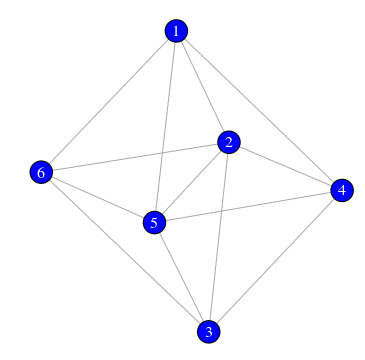
\includegraphics[scale=.4]{img/1.1_ejemplo_de_un_grafo_simple.png}
\par\bigskip
\small Fuente: Elaboración propia con \emph{igraph}
\end{minipage}\bigskip

Formalmente, definimos a un grafo y sus elementos de la siguiente manera:
\begin{definition}[Grafo]
\label{Grafo}
    Un \emph{grafo} $ G$ es un par $G = (V,E)$ de conjuntos tal que $E \subseteq [V]^{2}$; de modo que los elementos de $E$ son subconjuntos de 2-elementos de $V$. Los elementos de $V$ son llamados \emph{vértices}  del grafo $G$, los elementos de $E$ son sus \emph{aristas} escritas como \{$x,y$\}, $xy$ o $yx$\footnote{
	Ya que no se consideran grafos dirigidos en este trabajo, el orden en que son escritos los vértices conectados por aristas resulta indiferente.
    }. 
    Escribimos $V(G)$ para referirnos al conjunto de vértices y $E(G)$ para el conjunto de aristas de un grafo $G$\footnote{
	Estas convenciones son independientes de los nombres dados a los dos conjuntos; por ejemplo, el conjunto de vértices $W$ de un grafo $H = (W,F)$ será referido como $V(H)$.
	Por otro lado, si el conjunto de vértices admite una partición en $r$ clases, de acuerdo a la definición \ref{R_partitos} (\emph{grafos $r$-partitos}), se identificará cada clase de la partición (en un grafo, usualmente denotado $B$) con un subíndice de la forma: $V_{1}(B), V_{2}(B),..., V_{r}(B)$; cuyo orden es indicado por la suma del tamaño de cada clase: $N=n_{1}+n_{2}+...+n_{r}$.
    }. El número de vértices de un grafo $G$ es su \emph{orden}, escrito como $N = |G|=|V(G)|$ y el número de aristas es denotado por $M = ||(G)||=|E(G)|$.
\end{definition}

Una arista y un vértice son incidentes si la arista es conectada en uno de sus extremos a dicho vértice, formalmente:
\begin{definition}[Incidencia]
\label{Incidencia}
	Un vértice $x$ es \emph{incidente} con una arista $e$ si $x \text{ } \epsilon \text{ } e$.
\end{definition}

La conexión directa entre vértices es dada por una arista que los une, a esto se le conoce como \emph{adyacencia}; nombre que también se utiliza para aristas relacionadas por un vértice. Si dos vértices o aristas no son adyacentes, entonces son \emph{independientes}.
\begin{definition}[Adyacencia]
\label{Adyacencia}
	Dos vértices $x \neq y$ son \emph{adyacentes} entre sí si $xy \text{ } \epsilon \text{ } E(G)$. Dos aristas $e \neq f$ son \emph{adyacentes} si ambas son incidentes con un mismo vértice.
\end{definition}


\begin{definition}[Lazo y grafo simple]
\label{Lazo_GrafoSimple}
	Un \emph{lazo} es una arista donde el vértice inicial y el final son el mismo; es decir, $e=xx$. Decimos además que un grafo es \emph{simple} si no contiene lazos ni más de una arista entre cualquier par de vértices.
\end{definition}



Además de su representación gráfica o por medio de conjuntos, es posible describir completamente un grafo a través de su matriz de adyacencia, donde se especifica en la fila $i$ y columna $j$, si un vértice $v_{i}$ es adyacente con otro $v_{j}$.

\begin{definition}[Matriz de adyacencia]
\label{MatrizAdyacencia}
	La \emph{matriz de adyacencia} \textbf{A} = $(a_{ij})_{N \times N}$ de un grafo $G$ de orden $N$ está definida por:
	\[ a_{ij} = \left\{ \begin{array}{ll}
	    1 & \text{si } \{i,j\} \ \epsilon \ E(G)\\
	    0 & \text{en otro caso.}\end{array} \right. \]
\end{definition}
Como ejemplo, la matriz de adyacencia del grafo representado en la figura \ref{1.1_ejemplo_de_un_grafo_simple} ---donde la numeración con la que se ha nombrado a sus vértices corresponde a la posición de filas y columnas de la matriz--- es la siguiente:
\[
\begin{bmatrix}
    0 & 1 & 0 & 1 & 1 & 1\\
    1 & 0 & 1 & 1 & 1 & 1\\
    0 & 1 & 0 & 1 & 1 & 1\\
    1 & 1 & 1 & 0 & 1 & 0\\
    1 & 1 & 1 & 1 & 0 & 1\\
    1 & 1 & 1 & 0 & 1 & 0
\end{bmatrix}
\]
Aunque es usual que las relaciones entre actores en redes sociales sean descritas de esta forma simple, se puede modificar un poco la definición, estableciendo \emph{redes ponderadas}, en las que se asigna un \emph{peso} ---o importancia--- $w_{ij}$ a una relación entre dos actores.

\begin{definition}[Matriz de adyacencia ponderada]
\label{MatrizAdyacenciaPonderada}
    La \emph{matriz de adyacencia} \textbf{A} = $(a_{ij})_{N \times N}$ de un grafo $G$ ponderado de orden $N$ está definida por:
    \[ a_{ij} = \left\{ \begin{array}{ll}
	w_{ij} \neq 0 & \text{si } \{i,j\} \ \epsilon \ E(G)\\
	0 & \text{en otro caso.}\end{array} \right. \]
\end{definition}
Suponiendo que el grafo de la figura \ref{1.1_ejemplo_de_un_grafo_simple} fuese ponderado, se podría establecer una matriz de adyacencia como la siguiente:
\[
\begin{bmatrix}
    0   & 0.3 & 0    & 27   & 2.5  & 11\\
    0.3 & 0   & 1    & 3.4  & -1.1  & 4\\
    0   & 1   & 0    & 5    & 1    & 8.7\\
    27  & 3.4 & 5    & 0    & -2.1 & 0\\
    2.5 & -1.1& 1    & -2.1 & 0    & 1.4\\
    11  & 4   & 8.7  & 0    & 1.4  & 0
\end{bmatrix}
\]
Ya que una relación entre dos vértices $x$ e $y$ es descrita en un sentido $xy$ u otro $yx$ ---según la definición \ref{Grafo}---, la matriz que describe a un grafo será simétrica a lo largo de este trabajo.
Por otra parte, aunque la matriz de adyacencia para una red simple y ponderada se definen de la misma manera, hacemos una diferencia en la notación al referirnos por $a_{ij}$ a los elementos de una matriz binaria\footnote{
    La cual puede ser derivada de una matriz ponderada, usualmente representando la presencia ($w_{ij}\neq0$) o ausencia ($w_{ij}=0$) de una relación en la matriz original.
} y por $w_{ij}$ a los pesos de una matriz ponderada. 


Finalmente, como los grafos son descritos por conjuntos, es posible realizar operaciones y comparaciones a partir de ellos, algunas de las cuales son definidas a continuación.

\begin{definition}[Isomorfismo]
\label{Isomorfismo}
	Sean $G = (V,E)$ y $G' = (V',E')$ dos grafos. Decimos que $G$ y $G'$ son \emph{isomorfos} y escribimos $G \simeq G'$, si existe una biyección $\varphi: V \rightarrow V'$ con $xy \text{ } \epsilon \text{ } E \Leftrightarrow \varphi(x)\varphi(y) \text{ } \epsilon \text{ } E'$ para cada $x,y \text{ } \epsilon \text{ }V$. Tal mapeo $\varphi$ es llamado un \emph{isomorfismo}; si $G= G'$, es llamado un \emph{automorfismo}. Normalmente no hacemos distinciones entre entre grafos isomorfos. Por lo que escribimos $G=G'$ en lugar de $G \simeq G'$.
\end{definition}

\begin{definition}[Propiedad de grafo]
\label{Propiedad}
	Una clase de grafos que es cerrada bajo un isomorfismo es llamada una \emph{propiedad de grafo}. Por ejemplo, ``contener un triángulo'' es una propiedad de grafo: si $G$ contiene tres vértices adyacentes por  pares, entonces también los tienen cada grafo isomorfo a $G$.
\end{definition}


\begin{definition}[Subgrafo]
\label{Subgrafo}
	Sean $G=(V,E)$ y $G'=(V',E')$ dos grafos. Si $V' \subseteq V$ y $E' \subseteq E$, entonces $G'$ es un \emph{subgrafo} de $G$ (y $G$ es un supergrafo de $G'$), escrito como $G' \subseteq G$. Menos formalmente, decimos que $G$ \emph{contiene} a $G'$. Si $G' \subseteq G$ y $G' \neq G$, entonces $G'$ es un subgrafo propio de $G$.
\end{definition}


Si $U$ es un conjunto de vértices de $V(G)$ escribimos $G-U$ para $G[V \setminus U]$. En otras palabras, $G-U$ es obtenido al \emph{eliminar} de $G$ todos los vértices en $U \cap V$ y sus aristas incidentes. Si $U = \{v\}$, escribimos $G - v$ en lugar de $G - \{v\}$. Y en lugar de $G - V(G')$ escribimos simplemente $G - G'$. Para un subconjunto $F$ de $[V]^{2}$ escribimos $G - F := (V, E \setminus  F)$ y $G + F := (V, E \cup F)$. Como anteriormente, $G-\{e\}$ y $G+\{e\}$ es abreviado como $G-e$ y $G+e$. 


\begin{definition}[Maximal y minimal]
\label{MaximalMinimal}
	Llamamos a $G=(V,E)$ un \emph{arista maximal} con una propiedad dada si $G$ tiene dicha propiedad, pero no el grafo $G + xy$, para vértices no adyacentes $x,y \text{ } \epsilon \text{ } V$; de forma análoga, $G$ es un \emph{arista minimal} con una propiedad dada si $G$ tiene dicha propiedad, pero no el grafo $G - xy$. 
	Más generalmente, cuando llamamos a un grafo \emph{minimal} o \emph{maximal} bajo alguna propiedad ---ya sea para vértices o aristas--- pero no hemos especificado un orden particular, nos referimos a una relación con un subgrafo. Cuando hablamos de conjuntos minimales o maximales de vértices o aristas, nos referiremos simplemente a la inclusión de un conjunto.
\end{definition}



% BEGIN Sección 1.2.2
\subsection{Caminos y ciclos}
\label{sec:CaminosCiclos}

Conexiones sucesivas de aristas y vértices forman caminos y ciclos bajo los cuales se pueden estudiar relaciones que no son inmediatas, aquí se definen estos conceptos.

\begin{definition}[Camino]
\label{Camino}
	Un \emph{camino} es un grafo no vacío $P = (V,E)$ de la forma
	
	\begin{center}
	$V = \{x_{0},x_{1},...,x_{k}\} \hspace{4em} E = \{x_{0}x_{1},x_{1}x_{2},...,x_{k-1}x_{k}\}$,
	\end{center}
	
	donde los vértices $x_{i}$ son todos distintos. Los vértices $x_{0}$ y $x_{k}$ son \emph{unidos} por $P$ y son llamados sus \emph{finales}; los vértices $x_{1},...,x_{k-1}$ son los vértices \emph{interiores} de $P$. 
	El número de aristas de un camino es su \emph{longitud}, y el camino de longitud $k$ es denotado por $P^{k}$. Nótese que $k=0$ es permitido; por lo que $P^{0} = K^{1}$ ---ver definición \ref{GafoCompleto}---. 
	Denotaremos un camino por una de las secuencia naturales de sus vértices\footnote{De forma que: $x_{0}x_{1}...x_{k}$ y $x_{k}x_{k-1}...x_{0}$ denotan el mismo camino.}, escribiendo $P=x_{0}x_{1}...x_{k}$ y llamando a $P$ un camino \emph{de $x_{0}$ a $x_{k}$}.
\end{definition}


\begin{minipage}{\linewidth}
\centering
\captionof{figure}{Un camino $P = P^{6}$ en un grafo $G$} \label{1.2_CaminoP6}
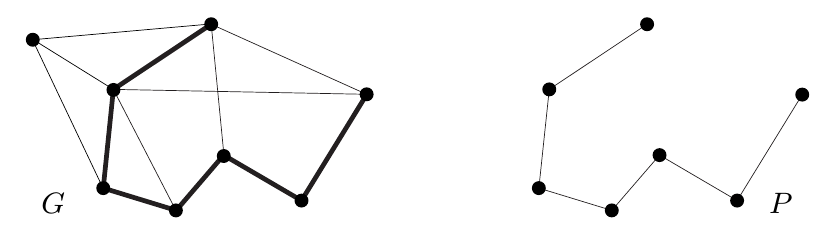
\includegraphics[scale=.3]{img/1.2_CaminoP6.png}
\par\bigskip
\small Fuente: \citep[6]{2005_Diestel_GraphThery}
\end{minipage}\bigskip


\begin{definition}[Ciclo]
\label{Ciclo}
	Si $P= x_{0}...x_{k-1}$ es un camino y $k \geq 3$, entonces el grafo $C:=P+x_{k-1}x_{0}$ es llamado un \emph{ciclo}. Como en los caminos, denotamos a un ciclo por la secuencia de sus vértices; el ciclo $C$ descrito anteriormente es escrito como $x_{0}x_{1}...x_{k-1}x_{0}$ o bien $x_{0}x_{k-1}...x_{1}x_{0}$. 
	La longitud de un ciclo también se define por su número de aristas; el ciclo de longitud $k$ es llamado un \emph{k-ciclo} y es denotado por $C^{k}$.
\end{definition}


\begin{definition}[Distancia]
\label{Distancia}
	La distancia $d_{G}(x,y)$ en $G$ de dos vértices $x,y$ es la longitud del camino más corto en $G$; si no existe dicho camino, entonces $d(x,y):= \infty$.
\end{definition}


Es importante mencionar que en grafos ponderados el concepto de longitud es asociado a la suma del peso de las aristas que conforman un camino o ciclo, estas longitudes ponderadas son utilizadas para establecer distancias mínimas diferenciadas en las ecuaciones \ref{eq:distanciaPonderada} y \ref{eq:distanciaAjustada}. 
De forma que ---a fin de evitar confusiones--- entenderemos el concepto de \emph{longitud} como el ``número de aristas en un camino o ciclo''; y para especificar el uso de los pesos en las aristas, elegiremos el término de \emph{longitud ponderada}.

Las distancia mínimas entre cada par de vértices genera una intuición en redes sociales de su ``distancia social'' y conectividad, que resulta fundamental para entender procesos de difusión. 
En redes reales se ha descrito una propiedad de ``mundo pequeño'' para señalar que a pesar de que una red registre una gran cantidad de vértices, generalmente existe un camino relativamente corto que los conecta. 
Sin embargo, ``el concepto de mundo pequeño, aunque intrigante, no es un indicio de un principio de organización particular'' \citep[49]{2002_Barabasi_MechanicsOfComplexNetworks}. 



% BEGIN Sección 1.2.3
\subsection{Grafos básicos}
\label{sec:GrafosBasicos}

Por su importancia teórica, algunos grafos han sido estudiados en detenimiento, ya que conforman topologías y características únicas que son de utilidad para establecer comparaciones y propiedades en subgrafos, aquí se presentan algunos de ellos que serán referidos en un análisis de redes posterior.

\begin{definition}[Grafo completo]
\label{GafoCompleto}
	Si todos los vértices de un grafo simple $G$ son adyacentes entre sí, entonces $G$ es un grafo \emph{completo}, escrito como $K^{N}$ para un grafo completo de orden $N$. 
	Un grafo $K^{3}$ es un \emph{triángulo}. 
	El número de aristas que contiene un grafo $K^{N}$ es:
	\begin{equation}
	 \frac{N(N-1)}{2}
	\end{equation} 
\end{definition}


\begin{definition}[Bosques y árboles]
\label{BosquesArboles}
	Un grafo \emph{acíclico} ---que no contiene ciclos--- es llamado un \emph{bosque}. Un bosque conectado ---ver definición \ref{Conectividad}--- es un \emph{árbol} (de modo que un bosque es un grafo cuyos componentes son árboles). Los vértices con una sola arista incidente en un árbol son sus \emph{hojas}. Cada árbol no trivial tiene al menos dos hojas.
\end{definition}


\begin{definition}[Grafos r-partitos]
\label{R_partitos}
	Sea $r \geq 2$ un entero. Un grafo $G = (V,E) $ es llamado \emph{r-partito} si $V$ admite una partición en $r$ clases, donde cada arista tiene sus finales en diferente clase: vértices en la misma clase no deben ser adyacentes. En lugar de ``2-partito'', generalmente decimos \emph{bipartito}.
\end{definition}


\begin{definition}[Grafos r-partitos completos]
\label{R_partitosCompletos}
	Un grafo r-partito en el que cada par de vértices de diferente clase particionada son adyacentes es llamado \emph{completo}; los grafos r-partitos completos para toda $r$ son \emph{grafos multipartitos completos}. 
	El grafo completo r-partito $\overline{ K^{n_{1}} } *... * \overline{ K^{n_{r}} }$\footnote{
	    La cardinalidad de cada clase es indicada de forma independiente, de forma que $n_{1}$ es el número de vértices pertenecientes a la primer clase dentro de la partición; $n_{2}$ el orden de la segunda clase, y así sucesivamente.
	} es denotado por $K_{n_{1},...,n_{r}}$. 
	Si $n_{1}=...=n_{r}=:s$, usamos la abreviación $K_{s}^{r}$; de modo que $K_{s}^{r}$ es el grafo r-partito completo en el que cada una de las $r$ clases dentro de la partición contiene exactamente $s$ vértices. 
	Grafos de la forma $K_{1,n}$ son llamados \emph{estrellas}.
\end{definition}

\begin{minipage}{\linewidth}
\centering
\captionof{figure}{Un grafo 3-partito y uno 3-partito completo} \label{1.3_Grafos_3partitos}
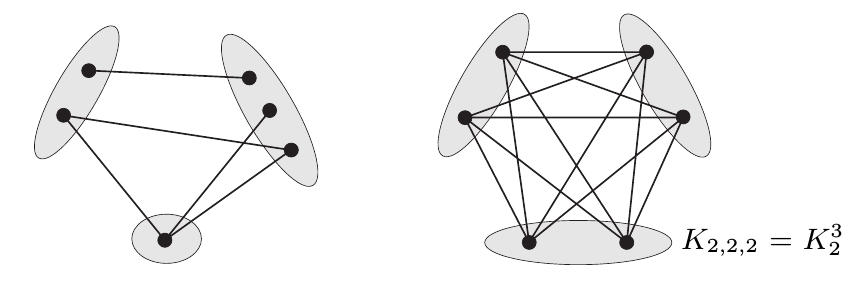
\includegraphics[scale=.3]{img/1.3_Grafos_3partitos.png}
\par\bigskip
\small Fuente: \citep[15]{2005_Diestel_GraphThery}
\end{minipage}\bigskip



% BEGIN Sección 1.2.4
\subsection{Características}
\label{sec:Caracteristicas}

Algunas de las características y propiedades topológicas de un grafo ---las más básicas--- son definidas aquí. 
Estas características son de especial ayuda para comprender de forma panorámica la estructura de un grafo.


\begin{definition}[Conectividad]
\label{Conectividad}
	Un grafo $G$ no vacío es llamado \emph{conectado} si cualesquiera dos vértices pueden ser unidos por un camino en $G$.
\end{definition}

\begin{definition}[Componente]
\label{Componente}
	Sea $G=(V,E)$ un grafo. Un subgrafo conectado maximal de $G$ es llamado una \emph{componente} de $G$. Nótese que una componente, al ser conectada es no-vacía; por lo que un grafo vacío no tiene componentes.
\end{definition}

\begin{definition}[Densidad]
\label{Densidad}
    Es el cociente dado por el número de aristas presentes en un grafo ($M$), entre el máximo número de aristas posibles, halladas en un grafo completo del mismo orden y tipo (por ejemplo: $N(N-1)/2$ en grafos simples, o $n_{1} \times n_{2}$ en un grafo bipartito). 
    Su valor varía de cero (ante la ausencia de aristas) a uno (grafo completo).
\end{definition}


\begin{definition}[Excentricidad]
\label{Excentricidad}
	La \emph{excentricidad} de un vértice $x$ es la máxima distancia\footnote{Se consideran sólo las distancias dentro de una componente, debido a que ---de acuerdo a la definición \ref{Distancia}--- dos vértices que pertenecen a diferentes componentes no tienen definida una distancia finita entre sí.} $d(x,y)$ entre $x$ y cualquier otro vértice del grafo, denotada por $\epsilon(x)$. 
	Formalmente, es escrita como: $\epsilon(x) = max_{y \text{ } \epsilon \text{ } V(G)} d(x, y)$.
\end{definition}


\begin{definition}[Diámetro]
\label{Diametro}
	La mayor distancia $d(x,y)$ entre dos vértices cualesquiera $x,y$ en $G$ es el \emph{diámetro} de $G$, denotado por $diam(G)$. Dicho de otra forma, es la máxima excentricidad en $G$, $diam(G)= max_{x \text{ } \epsilon \text{ } V(G)} \epsilon(x)$.
\end{definition}


\begin{definition}[Periferia]
\label{Periferia}
	La \emph{periferia} de un grafo es el conjunto de vértices cuya excentricidad es igual al diámetro del grafo; es decir, $\{x \mid \epsilon(x) = diam(G)\}$.
\end{definition}


\begin{definition}[Radio]
\label{Radio}
	El \emph{radio} de un grafo $G$ es la mínima excentricidad $\epsilon(x)$, calculada para $x \text{ } \epsilon \text{ } V(G)$. Formalmente, $rad(G) = min_{x \text{ } \epsilon \text{ } V(G)} \text{ } max_{y \text{ } \epsilon \text{ } V(G)} \text{ } d(x, y) = min_{x \text{ } \epsilon \text{ } V(G)} \epsilon(x) $.
\end{definition}


\begin{definition}[Centro]
\label{Centro}
	Un vértice $x$ es \emph{central} en $G$ si su excentricidad es igual al radio del grafo; es decir, $\{x \mid \epsilon(x) = rad(G)\}$.
\end{definition}

\begin{definition}[Distancia media entre vértices]
\label{Distancia media entre vértices}
    Denotada como $\ell$ y calculada para grafos con una sola componente como: 
    \begin{equation}\label{dist_media_1c}
	\ell=\frac{1}{N^2}\sum d(i,j)
    \end{equation} 
    o, en grafos con más de una componente (donde también se penalizan las ponderaciones de vértices en la periferia):
    \begin{equation}\label{dist_media_mc}
	\ell'=N(N-1) \left[ \sum_{i \neq j} \frac{1}{d(i,j)} \right]^{-1}
    \end{equation} 
    donde la distancia puede ser calculada por su longitud simple (de acuerdo a la definición \ref{Distancia}) o ponderada (ecuación \ref{eq:distanciaAjustada}).
\end{definition}

En términos matemáticos, el efecto de \emph{mundo pequeño} es descrito por \citet{2010_Newman_Networks} como la hipótesis de que la distancia media entre vértices\footnote{
    Aunque también se puede utilizar el diámetro del gafo, donde \citet{2010_Newman_Networks} describe que este exhibe un comportamiento similar, aún en grafos aleatorios, con $diam(G) \propto \log N$. 
} en una red simple crece proporcionalmente con el logaritmo de su orden (o resulta menor a este), es decir: $\ell \propto \log N$. 
Lo que en redes sociales usualmente implica la conexión de dos actores, no relacionados directamente, por medio de caminos compuestos por un pequeño número de conocidos. 







% BEGIN                                                                                                                                                          .                                                                                                                                                                        .                                              SECCIÓN 1.3 ANÁLISIS DE REDES                                                                                     .                                                                                                                                                                        .                                                                                                                                                                .
\section{Análisis de redes}
\label{sec:AnalisisRedes}

Hasta finales de los 90's, era común que los teóricos de grafos se preocupasen principalmente por cuestiones relacionadas con transiciones de fase, subgrafos y componentes gigantes; estudiando especialmente los casos cuando $N \rightarrow \infty$. 
Por su parte, los científicos sociales tenían dificultades para estudiar las redes constituidas por cientos de vértices, pero estaban fascinados con las propiedades de mundo pequeño, lazos débiles y estructuras de comunidades. 
Estas disciplinas, en conjunto con otras como la física ---interesada en conceptos universales de organización---, la biología ---enfocada en redes subcelulares---, la computación ---de perspectiva algorítmica--- y la ingeniería ---centrada en la exploración de redes de infraestructura--- abrieron una brecha por la que se ha consolidado el estudio de redes. 
Descrito como ``ciencia de redes'' ---y mencionado más comúnmente como ``análisis de redes''---, forma un campo de estudios multidisciplinario donde han sido adoptadas técnicas provenientes de diversos intereses particulares de investigación \citep[9 y 16]{2015_Barabasi_NetworkScience}. Para acercarnos al concepto de red, Newman proporciona una aproximación intuitiva:

\begin{center}
    \begin{minipage}{0.9\linewidth}
        {\setlength{\parindent}{12pt}\small
        El patrón de conexiones en un sistema dado puede representarse como una red, siendo los componentes del sistema los vértices de la red y las conexiones las aristas. 
        Después de reflexionar, no debe sorprendernos (aunque en algunos campos es un descubrimiento relativamente reciente) que la estructura de tales redes, el patrón particular de sus interacciones, puede tener un gran efecto en el comportamiento del sistema. (...) 
        A menos que sepamos algo sobre la estructura de estas redes, no podemos esperar comprender completamente cómo funcionan los sistemas correspondientes.
        
        Una red es una representación simplificada que reduce un sistema a una estructura abstracta, capturando sólo lo básico de sus patrones de conexión y un poco más. 
        Los vértices y las aristas en una red se pueden etiquetar con información adicional, como nombres o ponderaciones, para capturar más detalles del sistema, pero aún así generalmente mucha información se pierde en el proceso de reducir un sistema completo a una representación de red. 
        Esto ciertamente tiene sus desventajas pero también sus ventajas.  \normalsize \citep[11]{2010_Newman_Networks}.
        }
    \end{minipage}
\end{center}



Como en el caso de la teoría de grafos, la descripción que se hace de este campo no es del todo autocontenida\footnote{
En esta sección, los conceptos son retomados principalmente de \citet{2010_Newman_Networks} y \citet{1994_Wasserman_SNA}, se recomienda su consulta para profundizar en temas del análisis de redes y redes sociales que no han sido lo suficientemente desarrollados en este trabajo por cuestiones de espacio.}; 
por lo que nos centraremos principalmente en los fundamentos teóricos y técnicos que tienen una mayor implicación en nuestro estudio sobre redes de protesta. 


Un problema central al enfocarnos casi exclusivamente en redes r-partitas y ponderadas, reside en que las técnicas de análisis que han sido bien establecidas para redes simples no siempre se ajustan al considerar estos grafos\footnote{
    Según \citet{2013_Opsahl_BipartiteCluster}, redes bipartitas son raramente analizadas sin efectuar antes una transformación en ellas que las reduzca a redes simples o ponderadas. 
    En el caso de redes ponderadas, \citet{2004_Newman_WeightedNet} sugiere que las ponderaciones han recibido relativamente poca atención; algunas de las estrategias usuales para su análisis son: 
    (i) descartar los pesos asociados a las aristas, pese a la pérdida de información implicada; 
    (ii) considerar aristas paralelas análogas a los pesos asociados, si estos son enteros positivos; 
    (iii) aplicar las mismas métricas que en redes no ponderadas, si los resultados son justificables; 
    o (iv) definir nuevas métricas, que permitan lidiar específicamente con este tipo de redes.
}; 
aún así, adoptamos aquellos métodos cuyo empleo es justificado a partir del enfoque de este trabajo.




% BEGIN         SECCIÓN 1.3.1     REDES BIPARTITAS Y PROYECCIONES                                                                       .
\subsection{Redes bipartitas}
\label{subsec:redesBipartitas}

Una diferencia crucial en la representación de redes de afiliación descrita por \citet{1988_Breiger_Bipartite} y \citet{1994_Wasserman_SNA}, es la organización de los elementos en una matriz rectangular $\mathbf{B} = (b_{ij})_{n_{1} \times n_{2}}$. 
Donde $n_{1}$ filas pueden determinan actores sociales y $n_{2}$ columnas un conjunto de eventos. 
Cada elemento $b_{ij}$ será igual a uno si el actor $i$ participa en el evento $j$, y será igual a cero de otra manera; como en las redes ponderadas, se pueden establecer pesos que diferencien la fortaleza, distancia o costo de cada relación. 
Su representación como una matriz cuadrada también es posible, indicando tanto actores como eventos en filas y columnas de una matriz; sin embargo, esto sólo duplica la matriz original, sin proporcionar mayor información sobre dicha estructura y eventualmente no es computacionalmente eficiente:

\begin{equation}\label{eq:matriz_bipartita}
\mathbf{A} =     
\left[
\begin{matrix}
\mathbf{0} & \mathbf{B} \\
\mathbf{B^{T}} & \mathbf{0}
\end{matrix}
\right]
\end{equation} 


Debido a las limitaciones en las técnicas del análisis de redes bipartitas y ya que también resulta de interés estudiar de forma diferenciada las relaciones indirectas entre cada clase de la partición, se puede derivar una red simple o ponderada a través de una \emph{proyección}, que permite establecer relaciones, por ejemplo, de \emph{coparticipación} (entre actores) o por \emph{continuidad} (entre eventos). 
No obstante, esto no sólo ocasiona pérdidas de información ---al eliminar arbitrariamente una de las clases en la partición--- sino que puede resultar cuestionable, dado que supone la derivación de \emph{relaciones recíprocas directas} a partir de relaciones indirectas. 

En nuestro caso, hemos tomado el supuesto de que coaliciones de eventos son intencionales y derivadas de compromisos directos, adquiridos por cada uno de los actores colectivos que suscriben la protesta conjunta, de modo que una proyección entre actores resulta justificable ante tal presunción de colaboración; aún así, la proyección usualmente resultará menos informativa que la red bipartita original. 


Según \citet{2013_Opsahl_BipartiteCluster}, el método más simple de proyección implica la construcción de una red binaria simple; seleccionando una clase de la partición (supongamos actores) y estableciendo relaciones entre sus elementos si tienen en común al menos un vértice adyacente de la clase opuesta (por ejemplo, relacionando todos los actores que coparticipan en uno o más eventos comunes). 
Otras alternativas mantienen una estructura idéntica, pero los pesos entre las aristas se ajustarán por frecuencias de afiliación, de acuerdo al criterio adoptado. 
Entre estos criterios ponderados, consideramos: 

\begin{itemize}
    \setlength\itemsep{1em}
    \item \emph{Ponderación simple}. Donde cada relación es ponderada por el número de vértices adyacentes (en la clase descartada) que cada par de vértices de la clase seleccionada tienen en común. 
    Ya que toda ponderación $w_{ij}$ vinculada a una arista es discreta, también es posible definir aristas paralelas, que conectan un multigrafo. 
    En un contexto de proyección de relaciones indirectas entre actores, dada su coparticipación en eventos, este peso sugiere una frecuencia simple de asociaciones comunes entre actores. 
    Se puede calcular de forma simple como el producto matricial $\mathbf{G} = \mathbf{B}(\mathbf{B}^{T})$\footnote{
	La matriz $\mathbf{G}$ resultante sólo es asociada a relaciones entre actores; de forma análoga, una proyección ponderada simple sobre relaciones indirectas entre eventos, podría ser deducida por el producto matricial $\mathbf{G'} = \mathbf{B}^{T}(\mathbf{B})$.
    }, 
    donde la diagonal principal ---usualmente descartada bajo un principio que ignora la auto-acción \citep[87]{1988_Breiger_Bipartite}--- indicaría el número de eventos en los que ha participado cada actor. 
    
    
    
    \item \emph{Ponderación colaborativa}. Basada en la suposición de \emph{contribución marginal decreciente}; por ejemplo, si la contribución individual (aportada por cada actor) disminuye a medida que se incrementa el número de actores participantes en un evento colaborativo. 
    Así, si $n$ actores se relacionan por su coparticipación en una protesta particular, cada actor tendría una relación indirecta con $n-1$ actores. 
    Asumiendo que cada participante interactúa en la misma medida con otros actores, se asocia un peso de $1/(n-1)$ a cada arista derivada por dicha relación indirecta\footnote{
	De modo que la suma de los pesos de las aristas (creadas por adyacencia \emph{a un sólo vértice} de la clase opuesta) que conectan a un vértice con otros de su misma clase es igual a uno. 
	Esta, por supuesto, es una aproximación imprecisa, puesto que en la realidad las interacciones difícilmente se distribuyen uniformemente; pero podría ser nuestra mejor conjetura ante el desconocimiento sobre la fortaleza particular de cada relación. 
	Tal proyección ha sido deducida inicialmente en relaciones de coautoría para trabajos académicos, bajo el supuesto de que cada autor divide su tiempo equitativamente entre cada uno de sus coautores. 
	En el contexto de este trabajo, tiene coherencia suponer que un gran número de actores reportados en una protesta tienen una menor relación entre ellos (por ejemplo, en manifestaciones del día del trabajo, que suelen ser multitudinarias) que la que se podría deducir de una protesta suscrita sólo por unos pocos actores (usualmente con agendas más específicas).
    }. 
    Sumando todos los pesos asignados de esta manera para cada protesta, se obtendrían los pesos $w_{ij}$ de cada arista\footnote{
	Considerando el grafo bipartito (a la izquierda) en la figura \ref{1.4_ProyeccionesBipartitas}, el vértice de una clase diferente, adyacente a $A$, $B$ y $C$, genera tres aristas con un peso de 0.5 en la proyección de la derecha, que se mantienen inalterable para \{$A,C$\} y \{$B,C$\} al no existir más relaciones indirectas entre estos vértices; la arista \{$A,B$\} suma además el peso de otra relación indirecta, donde sólo participan este par de vértices (que genera un peso de 1), al añadirse al peso de la relación anteriormente considerada, obtenemos el valor 1.5 mostrado.
    }, de la forma: 
    \begin{equation}\label{eq:proyeccionNewman}
	w_{ij} = \sum_{p}\frac{\delta_{i}^{p} \delta_{j}^{p}}{n_{p}-1},
    \end{equation} 
    donde $n_{p}$ es el número de actores que coparticiparon en la protesta $p$; y $\delta_{i}^{p}$ resultaría igual a uno si el actor $i$ coparticipó en dicho evento $p$, y cero de otra forma (siendo $\delta_{j}^{p}$ un caso análogo para un actor $j$).
\end{itemize}




\hspace{-1em}\begin{minipage}{\linewidth}
\centering
\captionof{figure}{Una red bipartita (izquierda), proyección ponderada simple (centro) y proyección colaborativa (derecha).} \label{1.4_ProyeccionesBipartitas}
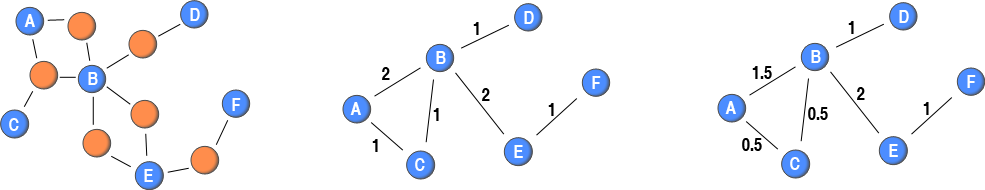
\includegraphics[scale=0.38]{img/1.4_ProyeccionesBipartitas.png}
\par\bigskip
\small Fuente: \url{https://toreopsahl.com/tnet/two-mode-networks/projection/}.
\end{minipage}\bigskip


\citet{2013_Opsahl_BipartiteCluster} sugiere dos defectos cruciales que se derivan de una proyección; en primer lugar, múltiples relaciones entre actores pueden ser creadas a partir de un sólo evento ---o viceversa---, por lo que su comparación con redes aleatorias (donde cada arista es generada de forma independiente) puede no resultar adecuada. 
En segundo lugar, dependiendo de la distribución de grado del conjunto de vértices no proyectados, la red proyectada puede generar más subgrafos completos que las redes simples, lo cual afecta las medidas para el coeficiente de clustering global y otras, principalmente aquellas basadas en triángulos ---ver definición \ref{GafoCompleto}---. 
\citet{1994_Wasserman_SNA} señalan por su parte que debido a que las redes de afiliación son definidas para subconjuntos (y no pares) de actores y eventos, existe pérdida de información y potenciales tergiversaciones cuando se estudian exclusivamente redes proyectadas. 



En algunas secciones de este capítulo presentamos medidas diferenciadas para analizar redes bipartitas que parten de nociones para el análisis de redes simples y que pueden ser utilizadas posteriormente para estudiar nuestra red de afiliación (dada por actores en eventos de protesta) y otra red bipartita de información agregada (entre tipos de actor y sus demandas). 
También se presentan métricas aplicables a una red ponderada proyectada entre actores. 

Específicamente, en las subsecciones \ref{subsec:centralidades} y \ref{sec:CoeficienteClustering}, se introduce cada método de análisis bajo el caso más simple, posteriormente se presentan ajustes para redes ponderadas y por último se describe su aplicación en redes bipartitas. 
Por su parte, las subsecciones \ref{sec:DistribucionCentralidades} y \ref{subsec:Comunidades} presentan métodos generalizados que son aplicables a distintos tipos de redes. 
Las subsecciones \ref{sec:EquivalenciaYSimilaridad} y \ref{subsec:Homofilia}, se centra principalmente en redes proyectadas unimodales; modelos nulos de referencia para tales proyecciones son fijados de acuerdo a la subsección \ref{sec:Redes_aleatorias_bipartitas}. 
El uso y comparación de estas medidas ofrece diferentes perspectivas sobre la topología y dinámica de las redes que se analizan más adelante. 




% BEGIN         SECCIÓN 1.3.2     MEDIDAS DE CENTRALIDAD                                                                       .
\subsection{Medidas de centralidad}
\label{subsec:centralidades}
Un método básico del análisis de redes para determinar algunas de las propiedades estructurales en un grafo consiste en evaluar la importancia o \emph{centralidad} relativa de cada vértice. 
Dicha importancia no es definida de forma única, sino a través de distintas métricas que caracterizan centralidades entorno a: número e importancia de relaciones (centralidad de grado, eigenvalor y Katz), capacidad para alcanzar a los otros vértices de la red (centralidad de cercanía) y su función como intermediario entre otros vértices (centralidad de intermediación). 
Centralidades adicionales han sido definidas para medir otras características o casos más específicos; sin embargo, nos centramos sólo en estas medidas ---de uso frecuente---, utilizadas posteriormente en nuestro análisis.


\subsubsection{Grado}
\label{sec:centralidadGrado}

Según \citet{2010_Newman_Networks}, es razonable suponer que aquellas unidades sociales que tienen una mayor cantidad de relaciones resulten beneficiadas al obtener una mayor influencia directa, acceso a la información y prestigio que aquellas que tienen pocas conexiones. 
Bajo esta premisa, para determinar la centralidad de un vértice (de acuerdo al número e importancia de sus relaciones inmediatas) se calcula su \emph{grado}; en grafos simples este se define al contar el número de aristas $a_{ij}$ ---ver definición \ref{MatrizAdyacencia}--- incidentes en un vértice $i$:
\begin{equation}\label{k_i}
    k_{i} = C_{D}(i) = \sum_{j=1}^{N}a_{ij}. 
\end{equation} 
Sin embargo, en redes ponderadas también se pueden considerar los pesos $w_{ij}$ ---de acuerdo a la definición \ref{MatrizAdyacenciaPonderada}--- asignados a las aristas incidentes al vértice $i$. 
Este grado ponderado $s_{i}$ es asociado a la \emph{fortaleza} de un vértice, cuya interpretación en redes sociales puede ser vinculada a la teoría de \citet{1983_Granovetter_WeakTies} sobre  relaciones fuertes o débiles. 
Una medida que ha sido utilizada frecuentemente, consiste en sumar todos los pesos de las aristas incidentes de la forma: 
\begin{equation}\label{s_i}
    s_{i} = C_{D}^{w}(i) = \sum_{j=1}^{N}w_{ij}.
\end{equation} 
Para \citet{2004_Newman_WeightedNet}, esta es una medida razonable para medir influencia social; sin embargo, \citet{2010_Opsahl_NodeCentralityWeighted} sugieren que al considerar el grado sólo como la suma de los pesos, se ignora el componente original de la medida (el número de relaciones incidentes en un vértice). 
De modo que proponen la métrica de la ecuación \ref{eq:degreeCentrality}, que permite un ajuste entre las ecuaciones \ref{k_i} y \ref{s_i}.

\begin{definition}[Centralidad de grado ajustada]
\label{CentralidadGrado}
    La \emph{centralidad de grado ajustada} en una red ponderada para un vértice $i$, será el producto entre el número de vértices adyacentes $k_{i}$ y el peso de las aristas incidentes en él, ajustado por un parámetro $\alpha \text{ } \epsilon  \text{ } $ [0,1]\footnote{
	El rango es colocado de forma que se favorece la incidencia de múltiples relaciones débiles sobre la de pocas relaciones fuertes. De otra forma, el rango debería ser colocado por encima de 1 ---\citet{2010_Opsahl_NodeCentralityWeighted}---.
    }. Formalmente:
    \begin{equation}\label{eq:degreeCentrality}
	C_{D}^{w \alpha}(i) = k_{i} \times \left( \frac{s_{i}}{k_{i}} \right) ^{\alpha} = k_{i}^{(1-\alpha)} \times s_{i}^{\alpha},
    \end{equation} 
    donde el parámetro $\alpha$ en la ecuación \ref{eq:degreeCentrality} será determinado por el tipo de red que se analice, permitiendo variar la importancia entre el número aristas incidentes a un vértice y los pesos de las mismas. 
    Se puede ver que si $\alpha = 0 $ entonces $ C_{D}^{w \alpha}(i) = k_{i} $, y si $\alpha = 1 $ entonces $ C_{D}^{w \alpha}(i) = s_{i} $. 
    Ya que estos valores no se calculan dentro de un rango máximo, sólo serán significativos en términos relativos.
\end{definition}


Una práctica común en redes simples consiste en normalizar el grado de cada vértice al acotarlo (entre cero y uno), dividiendo el valor en la ecuación \ref{k_i} por un máximo relativo, de la forma $k_{i}/(N-1)$, de modo que estas centralidades sean comparables entre grafos de cualquier orden  
Siguiendo esta idea, en redes bipartitas no ponderadas de orden $N = n_{1} + n_{2}$, \citet{1997_Borgatti_2ModeSNA} sugieren que el grado de cada vértice sea normalizado por el número de vértices de la clase opuesta ($n_{1}$ o $n_{2}$), que a su vez constituye un máximo relativo. 
Pese a que esta normalización no produce una transformación lineal (al contrario de lo sucedido para redes simples), su ventaja radica en hacer comparables los grados de cada vértice en la red. 




\subsubsection{Cercanía}
De acuerdo a \citet{2010_Newman_Networks}, en redes sociales, un actor que puede ser conectado con otros a través de un camino relativamente corto podría tener mayor acceso a la información (que se produce fuera de un ambiente local) o una influencia más directa a otros vértices en la red; así mismo, una alta \emph{cercanía} en unidades sociales que caractericen demandas o actores podría implicar facilidades para que las agendas involucradas a tales unidades se propaguen. 
De forma general, la medida de cercanía toma en consideración la estructura global de la red, ya que suma las distancias $d(i,j)$ ---ver definición \ref{Distancia}--- entre un vértice $i$ y los otros $j$ pertenecientes al mismo grafo. 
Formalmente es referida como el recíproco de la suma de estas distancias:
\begin{equation}\label{eq:cercania_simple}
    C_{C}(i) = \left[ \sum_{j=1}^{N} d(i,j) \right]^{-1}.
\end{equation}
No obstante, \citet{2010_Newman_Networks} identifica que en la práctica las centralidades de cercanía (a diferencia de otros índices) tienden a ser similares, debido a que las distancias en redes reales suelen ser cortas, de modo que puede resultar difícil distinguir entre vértices más centrales. 


Existen varios algoritmos para calcular distancias; debido a que varias de nuestras redes son proyecciones ponderadas, consideramos el algoritmo de 
\citet{1959_Dijkstra_TwoProblems}, que calcula el camino más corto en este tipo de redes. 
Sin embargo, su método en una implementación común considera los pesos asociados a las aristas como su longitud y calcula cada distancia como la suma de los pesos asignados a las aristas que conforman el camino de menor peso total. 
Ya que en la interpretación usual de redes sociales se asocia un mayor peso a una relación más cercana entre vértices, se ha propuesto asignar el recíproco de los pesos antes de utilizar el algoritmo de Dijkstra; así la distancia (referida como \emph{costo de interacción}) sería calculada como la suma mínima de los pesos recíprocos de las aristas que forman un camino del vértice $i$ al $j$:
\begin{equation}\label{eq:distanciaPonderada}
    d^{w}(i,j) = min\left( \frac{1}{w_{ih}}+...+ \frac{1}{w_{hj}} \right).
\end{equation}

Existen dos consideraciones sobre las distancias, interpretadas como costos de interacción en una red social: ``Primero, un gran número de vértices interiores incrementa el tiempo invertido en la interacción entre dos vértices. Segundo, los vértices interiores están en una posición de \emph{tertius gaudens}\footnote{Las cursivas son propias. La expresión, en latín es traducida como ``tercero que se alegra'' y es aplicable cuando una parte ajena resulta beneficiada de la interacción o rivalidad entre dos partes.} o poder de terceras partes, y puede distorsionar información o retrasar la interacción entre los vértices.'' ---\citet{2010_Opsahl_NodeCentralityWeighted}---\footnote{
    La traducción ha considerado la adecuación a las definiciones dadas en este texto.
}. 
Un defecto crucial en la ecuación \ref{eq:distanciaPonderada} es que la distancia puede ser determinada sin ejercer ningún control sobre el número de vértices interiores (puesto que sólo se usa un criterio asociado al peso). 
Como alternativa, \citet{2010_Opsahl_NodeCentralityWeighted} proponen una modificación a los pesos asignados, donde se penalice a un gran número de vértices interiores. 
Para ello, se deberá reemplazar el peso original de cada arista por su recíproco, ajustado por un parámetro $\alpha \text{ } \epsilon \text{ } [0,1] $; de forma que la distancia dada por el algoritmo de Dijkstra es calculada como:
\begin{equation}\label{eq:distanciaAjustada}
    d^{w \alpha}(i,j) = min\left( \frac{1}{(w_{ih})^{\alpha}}+...+ \frac{1}{(w_{hj})^{\alpha}} \right),
\end{equation}
como en el caso del grado de un vértice, el parámetro de ajuste $\alpha$ puede variar, de modo que se determina para cada tipo de red según su pertinencia al dar mayor importancia al peso entre relaciones (cuando $\alpha \rightarrow 1$) o al menor número de vértices interiores (cuando $\alpha \rightarrow 0$). 
Finalmente, se determinará la \emph{centralidad de cercanía} de un vértice $i$ usando estos pesos de la forma:
\begin{equation}\label{eq:cercaniaAjustada}
    C_{C}(i) = \left[ \sum_{j=1}^{N} d^{w \alpha}(i,j) \right]^{-1}.
\end{equation}
Al añadir información sobre la fortaleza de una relación se puede esperar un mayor rango en la distribución dada por esta centralidad, pero esto dependerá de la variabilidad en las ponderaciones asociadas a las aristas. 


Ya que dos vértices que pertenecen a una diferente componente no tienen definida una distancia finita entre ellos, es usual que en grafos no conectados sólo se calcule la centralidad en la componente que conecta la mayor parte de los vértices del grafo. 
Una alternativa, referida por \citet{2010_Newman_Networks}, que resulta congruente para un grafo con múltiples componentes, consiste en calcular esta centralidad como la suma de las distancias inversas, con la convención de que $1/\infty =0$ y excluyendo $i=j$: 
\begin{equation}\label{eq:cercaniaAjustada2}
    C_{C}'(i) = \sum_{j=1}^{N} \frac{1}{d^{w \alpha}(i,j)}.
\end{equation}
Además de permitir calcular la centralidad de cercanía de todos los vértices en una red con múltiples componentes, esta medida asigna un mayor peso a los vértices que están cerca de $i$ que aquellos que están lejos, cuyas contribuciones marginales son cercanas a cero. 

Como en la centralidad de grado, en redes simples se suele normalizar su valor al multiplicar la ecuación \ref{eq:cercania_simple} por $N$\footnote{
    En realidad $N-1$ es el mínimo valor posible, ya que la distancia de un vértice a sí mismo es igual a cero; sin embargo autores como \citet{2010_Newman_Networks} recomiendan la normalización por el orden del grafo ya que ``tiende a dar resultados analíticos ligeramente más elegantes''.
}, interpretando este índice como el recíproco de la distancia promedio a todos los otros vértices. 
De nuevo, \citet{1997_Borgatti_2ModeSNA} proponen una normalización a modo para una red bipartita simple de orden $N = n_{1}+n_{2}$. 
Ya que la distancia mínima a cada vértice de la clase opuesta es igual a uno, y (consecuentemente) la distancia a vértices de su misma clase sería de al menos dos; la centralidad de cercanía mínima sería (considerando vértices de la clase $V_{1}(B)$\footnote{
    De otra forma, la cercanía mínima sería igual a $n_{1}+2n_{2}-2$. 
}) igual a $n_{2}+2n_{1}-2$, cuyo valor es multiplicado (según clase a la que pertenezca cada vértice) para cada cercanía calculada.



\subsubsection{Intermediación}
La intermediación pretende determinar la importancia que tiene un vértice como conector en la red; de modo que, si su valor para un vértice $i$ es alto, gran parte de los caminos más cortos que conectan a los vértices $j \text{ } \epsilon \text{ } V$ con otros diferentes $k \text{ } \epsilon \text{ } V$, tienen a $i$ como vértice interior.
De forma general, una alta centralidad de intermediación en distintas unidades sociales puede revelar control sobre la información u otros procesos propagables en la red ---\citet{2010_Newman_Networks}---. 
Más específicamente, al considerar actores en protestas podríamos comprobar si la observación de \citet{2003_Wada_Tesis} sobre la capacidad de ONGs para interconectar actores multisectoriales en México resulta válida para nuestra evidencia. 


Formalmente, la intermediación de un vértice $i$ se define como el cociente entre el número de caminos más cortos que tienen a $i$ como vértice interior y el número total de caminos más cortos, como refiere \citet{2010_Opsahl_NodeCentralityWeighted}:
\begin{equation}\label{eq:intermediacion}
    C_{B}^{w \alpha}(i) = \sum_{i \neq j \neq k} \frac{g_{jk}^{w \alpha}(i)}{g_{jk}^{w \alpha}},
\end{equation}
donde los caminos más cortos en una red ponderada son determinados de acuerdo a la ecuación \ref{eq:distanciaAjustada}.

En grafos simples, la normalización de la ecuación \ref{eq:intermediacion} puede considerar una división entre el máximo valor posible: $(N-1)(N-2)/2$ ---que es el número de pares de vértices que no incluyen a $i$---. 
Según \citet{1997_Borgatti_2ModeSNA}, la normalización de esta centralidad en un grafo bipartito $B$ de orden $N = n_{1}+n_{2}$, depende dos factores; en primer lugar de la clase a la que pertenezca un vértice, y en segundo lugar del tamaño relativo de cada clase. 
Considerando, por ejemplo, el índice de intermediación de un vértice en la clase $V_{1}(B)$, este es normalizado al dividirlo por el máximo relativo, dado por: 
\begin{equation}\label{eq:intermediacion_normalizada}
\begin{cases} 
    2(n_{1}-1)(n_{2}-1)  &  \text{ si } n_{1} > n_{2},\\ 
    \frac{1}{2}n_{2}(n_{2}-1) + \frac{1}{2}(n_{1}-1)(n_{1}-2) + (n_{1}-1)(n_{2}-1) & \text{ si } n_{1} \leq n_{2}.
\end{cases}
\end{equation}
cambiando los subíndices para vértices de la clase $V_{2}(G)$.



\subsubsection{Centralidad de vector propio}
\label{sec:Centralidad_vector_propio}

Una limitación de la centralidad de grado radica en que la importancia de un vértice es establecida sólo en función de sus vértices adyacentes; es decir, de su ambiente local. 
Como alternativa, la \emph{centralidad de vector propio} calcula la importancia de un vértice en función de la importancia de sus vértices adyacentes, definiendo a su vez esta importancia de forma recursiva, asociando a cada vértice una centralidad proporcional a la suma de las centralidades de sus vértices adyacentes \citep[169--172]{2010_Newman_Networks}. 
En redes sociales, se puede inferir que la importancia de un vértice (caracterizada por este índice) depende en gran medida de la importancia de las unidades sociales a las que está conectado. 

Según esta aproximación intuitiva, la centralidad de vector propio puede ser obtenida bajo una serie de $t$ iteraciones; asignando un valor inicial (en $t=0$) a la centralidad relativa $x_{j} > 0$ de cada vértice $j$:

\begin{equation}\label{eigenvalue_intuitivo}
    x_{i}(t) = \sum_{j} A_{ij}x_{j}(t),
\end{equation}
donde $t$ es el número de iteración, $A_{ij}$ son los valores de la matriz de adyacencia (con entradas no negativas) y $x_{j}(t) = x_{i}(t-1)$ para $i=j$ y $t>0$. 


Con cada iteración se propaga gradualmente la suma de los pesos de los vértices adyacentes. 
Sin embargo, cuando $t \rightarrow \infty$, los valores $x_{i}(t)$ de la ecuación \ref{eigenvalue_intuitivo} pueden continuar creciendo indefinidamente, de modo que se ajusta cada uno de los valores por un escalar $1 / \lambda$:
\begin{equation}\label{eigenvalue_largo}
    x_{i}(t) = \dfrac{1}{\lambda}\sum_{j} A_{ij}x_{j}(t),
\end{equation} 
esta vez, los valores de $x_{i}(t)$ en la ecuación \ref{eigenvalue_largo} convergen a valores no negativos cuando $t \rightarrow \infty$\footnote{
    Tal como es descrito este proceso, se asocia la centralidad de vector propio a una caminata aleatoria de longitud infinita, en la que cada vértice es elegido uniformemente del conjunto de vértices adyacentes al vértice seleccionado en el momento $t$; de modo que la centralidad de vector propio converge a la \emph{distribución estacionaria} de la caminata aleatoria. 
    [Fuente: \emph{Kamesh Munagala, Lecture 12 : Random Walks and Graph Centrality (28 de Febrero, 2017) pag. 2.} Disponible en: \url{https://users.cs.duke.edu/~kamesh/ModernAlg/lec8.pdf}, consultado el 23 de junio de 2018].
}. 
Podemos abreviar dicha expresión de forma general, para el vector convergente $\mathbf{x}$ en forma matricial como:
\begin{equation}\label{eigenvalue_centrality}
    \mathbf{A} \mathbf{x} = \lambda \mathbf{x},
\end{equation}
la cual es la ecuación de vector propio de la matriz de adyacencia $\mathbf{A}$, donde $\mathbf{x}$ (a veces llamado \emph{vector propio principal}) es el vector propio asociado al mayor de los valores propios $\lambda$ que satisfacen la ecuación\footnote{
Este valor propio es elegido como consecuencia del teorema Perron--Frobenius. 
Ya que todos los valores en $\mathbf{x}$ deben ser no negativos, sólo el mayor valor propio genera los valores de centralidad buscados. 
}. 
Por supuesto, se puede usar álgebra lineal para calcular los vectores propios de la matriz de adyacencia; sin embargo, no es considerado un método eficiente. 
En su lugar, es común que se utilice el algoritmo iterativo descrito aquí (referido como \emph{power iteration} o \emph{Von Mises iteration})\footnote{
    Al respecto, \citet{2010_Newman_Networks} realiza las siguientes advertencias: 
    (i) el vector inicial no debe ser ortogonal al vector propio principal, lo cual puede ser evitado eligiendo un vector inicial con entradas positivas 
    (ii) ya que los elementos del vector calculado crecen gradualmente con cada iteración, se deben normalizar periódicamente para evitar números arbitrariamente grandes 
    (iii) una forma simple de detener las iteraciones es establecer un umbral de tolerancia para la diferencia entre dos vectores iniciales calculados de forma paralela. 
    Varias implementaciones de este algoritmo han sido programadas para casi cualquier paquete de análisis de redes.
} donde los valores iniciales pueden ser aleatorios o aproximaciones al vector propio principal. 


Cada valor de $\mathbf{x}$ es la centralidad de vector propio asociada a un vértice de la red. 
Un mayor valor es consecuencia de una alta centralidad para un vértice, ya sea debido a que este se relacione a muchos otros, a vértices que a su vez tienen alta centralidad o porque los pesos asociado a sus aristas incidentes son elevados. 
Considerando pesos enteros positivos, Newman justifica la utilización de esta medida para redes ponderadas:

\begin{center}
    \begin{minipage}{0.9\linewidth}
        {\setlength{\parindent}{12pt}\small
        Los vértices en una red que son adyacentes a un vértice con el doble de peso contribuyen 
        (...) el doble de la centralidad de vector propio del vértice. 
        Como resultado, encontramos que la generalización correcta de la centralidad de vector propio en una red ponderada es, como sería de esperar, aún el vector propio principal de la matriz de adyacencia, siendo los elementos de la matriz iguales a los pesos de las aristas \normalsize \citep[2]{2004_Newman_WeightedNet}.
        }
    \end{minipage}
\end{center}



Su interpretación en una red de coparticipación entre actores y eventos, según \citet{1997_Borgatti_2ModeSNA}, implica que la centralidad de los actores será determinada por la suma de las centralidades de los eventos en los que coparticipan y, simultáneamente, la centralidad de los eventos es determinada por la suma de las centralidades de los actores que coparticipan en ellos. 
Esta doble implicación supone ---como ya han sugerido \citet{1993_BrmanEvtt_StructureSocialProtest}--- una relación recíproca entre protestas y actores exitosos; de modo que actores relevantes estarán vinculados a eventos relevantes y viceversa.



\subsubsection{Centralidad de Katz}
\label{sec:Centralidad_Katz}

Una alternativa a la centralidad de vector propio es establecida en la centralidad propuesta por \citet{1953_Katz_centrality}, donde se ajusta un factor de atenuación para vértices conectados por un camino de acuerdo a su longitud. 
Aplicado, por ejemplo, a la transmisión de mensajes o influencia a través de una red social, se puede suponer que su propagación a través de un camino de longitud $k$, tiene una probabilidad $\alpha^{k}$ de ser efectivo. 
Es decir, su eficacia se reduce a una mayor distancia\footnote{
La formulación original de \citet{1953_Katz_centrality} traduce esta idea de forma directa bajo la expresión: 
$\mathbf{T} = \alpha \mathbf{A} + \alpha^2 \mathbf{A}^2 + \cdots + \alpha^k \mathbf{A}^k + \cdots 
= \sum_{n=1}^{\infty}(\alpha \mathbf{A})^n$;
a partir de la cual (mediante álgebra matricial) llega a una expresión similar a la que presentamos aquí, pero que es deducida más intuitivamente por \citet{2010_Newman_Networks}, por lo que referimos ésta última.
}.


Para deducir la centralidad de Katz se puede comenzar con una expresión similar a la ecuación \ref{eigenvalue_largo}, que presentamos para la centralidad de vector propio:
\begin{equation}\label{formulacion_katz}
    x_{i}(t) = 
    \alpha \sum_{j} A_{ij}x_{j}(t) + \beta,
\end{equation} 
o en notación matricial: 
\begin{equation}\label{formulacion_katz2}
    \mathbf{x} = 
    \alpha \mathbf{Ax} + \beta\mathbf{u},
\end{equation} 
despejando para $\mathbf{x}$:
\begin{equation}\label{formulacion_katz3}
    \mathbf{x} = 
    \beta(I-\alpha \mathbf{A})^{-1} \cdot \mathbf{u},
\end{equation} 
donde los parámetros $\alpha$ y $\beta$ son constantes positivas y $\mathbf{u}$ es un vector que contiene sólo elementos unitarios; $\alpha$ es un factor de atenuación y $\beta$ es una centralidad adicional que cada vértice recibe. 
Ya que los valores de centralidad sólo son significativos relativamente, su valor absoluto no es importante ---el parámetro $\beta$ en la ecuación \ref{formulacion_katz3} sólo multiplica su valor--- por lo que usualmente se asigna $\beta=1$\footnote{
La utilidad del parámetro $\beta=1$ es notoria sólo para redes acíclicas, donde la centralidad de vector propio resulta inútil. 
En otros casos, se pueden asignar ponderaciones iniciales diferentes a la unidad ---cuando se tiene información adicional sobre los vértices que afecte su centralidad--- por medio de un vector ponderado, en lugar de la combinación $\beta\mathbf{u}$ en la ecuación \ref{formulacion_katz2}. 
}, lo que resulta en la centralidad de Katz:

\begin{equation}\label{eq:centralidad_katz}
    \mathbf{x} = 
    (I-\alpha \mathbf{A})^{-1} \cdot \mathbf{u}.
\end{equation} 


Donde se debe determinar un valor adecuado para $\alpha$ con el fin de obtener el vector solución. \citet{2010_Newman_Networks} indica que $\alpha$ debe ser mayor a cero y menor que el recíproco del valor propio $\lambda_l$ más grande de $\mathbf{A}$ para converger\footnote{
    Si $a \rightarrow 0$ todos los vértices tendrán la misma centralidad (igual a $\beta$). 
    Conforme se incrementa su valor, las centralidades aumentan hasta que divergen cuando $det(\mathbf{A}-\alpha^{-1}\mathbf{I})=0$; es decir, la condición expresa la ecuación característica (equivalente a la ecuación \ref{eigenvalue_centrality}) cuyas raíces $\alpha^{-1}$ son iguales a los valores propios de la matriz de adyacencia. 
    Conforme $\alpha$ se incrementa, el primer determinante en romper la condición ocurre para el valor propio más grande ($\alpha^{-1}= \lambda_{l}$). 
}. 
En la práctica, señala que se utilizan valores cercanos al máximo $1 / \lambda_{l}$, lo cual devuelve valores cercanos a la centralidad de vector propio, pero donde se reduce la ponderación para vértices que no están en componentes fuertemente conectadas.

La centralidad de Katz puede calcularse invirtiendo la matriz en la ecuación \ref{eq:centralidad_katz} (lo cual no es computacionalmente óptimo) o a través de iteraciones sucesivas, indicando una centralidad inicial (para $t=0$) y calculando sucesivamente los valores en la ecuación \ref{formulacion_katz} hasta la convergencia. 
Esta centralidad sólo es utilizable en redes simples unimodales. 



% BEGIN         SECCIÓN 1.3.3     DISTRIBUCIÓN DE MEDIDAS DE CENTRALIDAD                                                                       .
\subsection{Distribución de medidas de centralidad}
\label{sec:DistribucionCentralidades}

Ya que cada medida de centralidad es un índice discreto calculado para todo vértice, sus observaciones pueden ser agrupadas en una distribución de frecuencias, la cual puede ser asociada a su vez a una distribución de probabilidad (discreta o continua) que comprende frecuencias teórica que caracterizan la variabilidad de resultados esperados a partir de los datos experimentales analizados. 
Vistas como características generales sobre la estructura de una red, las distribuciones de las medidas de centralidad nos ofrecen una aproximación panorámica fundamental. 


Operativamente, cada distribución de centralidad experimental $P_{exp}(x)$ en la red analizada es establecida por la fracción de vértices $n_{x}$ que tienen una centralidad $x$. 
Por ejemplo, la distribución de la centralidad de grado simple es obtenida (de acuerdo a la ecuación \ref{k_i}) a través de:
\begin{equation}\label{eq:distribucion_grado}
    P_{exp}(k) = \frac{n_{k}}{N}, 
\end{equation}
de tal manera que cada valor calculado puede ser visto como la probabilidad de que un vértice, elegido al azar en la red, sea incidente a $k$ aristas. 
Donde esta perspectiva ha resultado útil para crear modelos teóricos de redes. 


\subsubsection{Distribución de grado}
\label{subsubsec:Distribuciob_grado}
Según \citet{2010_Newman_Networks}, casi todas las \emph{distribuciones de grado} deducidas en aplicaciones reales tienen una distribución sesgada a la derecha; es decir, que pocos vértices (distribuidos en un rango amplio) poseen un grado superior a la media. 


En redes con una gran cantidad de vértices, dicha distribución se intenta ajustar comúnmente a una \emph{distribución de ley de potencia}\footnote{
    Según Albert \& Barabási, ``el descubrimiento de la distribución de ley de potencia ha llevado a la construcción de varios modelos con esta distribución de grado que, al centrarse en la dinámica de la red, apuntan a ofrecer una teoría universal de la evolución de redes'' \citep[49]{2002_Barabasi_MechanicsOfComplexNetworks}. 
    Esta estructura fue inicialmente descubierta en la Internet y a partir de entonces se han analizado otras redes complejas en economía, lingüística, negocios, relaciones sexuales, interacciones sociales, citaciones académicas y redes biológicas entre otras, donde la mayor parte de ellas siguen una distribución de ley de potencia, de acuerdo a la ecuación \ref{eq:scale-free}, con valores típicos de 2 $\leq \alpha \leq$ 3, aunque valores ligeramente diferentes son observables ocasionalmente ---\citet{2010_Newman_Networks}---.
}, 
que involucra un sesgo mucho más amplio, donde sólo con unos cuantos vértices (denominados \emph{hubs}) mantienen una gran cantidad de relaciones, mientras que otros vértices (la mayoría) posee muy pocas conexiones. 
Su formulación en redes simples indica que la probabilidad de que cualquier vértice esté conectado a otros $k$ vértices es proporcional a $1/k^{\alpha}$: 
\begin{equation}\label{eq:scale-free}
    P(k) \sim k^{-\alpha}.
\end{equation}
Sin embargo, es común que la distribución de frecuencias en datos experimentales no resulte decreciente según la ecuación \ref{eq:scale-free} para cualquier grado, ajustándose adecuadamente sólo en cierto rango de observaciones (especialmente a partir de cierto grado $k$). 
Aún así, redes que presentan un ajuste razonable en un rango considerable de frecuencias, han sido llamadas \emph{redes libres de escala} (por la divergencia teórica de sus momentos). 


Un reconocimiento visual puede ser intuitivo y regresiones lineales sobre la distribución de grado (en escalas logarítmicas) han sido utilizadas para determinar si una red tiene una distribución de grado libre de escala. 
Sin embargo, \citet{2009_PowerLaw_Clauset_EtAl} y \citet{2010_Newman_Networks} indican que este último método (y variaciones del mismo) genera errores sistemáticos significativos. 
En su lugar, \citet{2009_PowerLaw_Clauset_EtAl} sugiere un estimador de máxima verosimilitud para probar la consistencia de la hipótesis de una distribución de ley de potencia. 
Siempre y cuando el número de observaciones ---distintos grados $k$--- no sea demasiado pequeño (número de observaciones $ \gtrsim 100$) para permitir una clara distinción respecto a otros ajustes en distribuciones de probabilidad alternativos (por ejemplo, exponenciales o log-normales). 

La variación de centralidades de grado en las redes que analizamos no es lo suficientemente grande para intentar aproximar una distribución libre de escala, por lo tanto sólo tomamos como referencia a esta distribución, la cual sugiere (según el modelo de Barabási-Albert) que el crecimiento de una red amplia es determinado por un ``apego preferencial'', que implicaría la \emph{preferencia} potencial de nuevas unidades sociales por crear y mantener relaciones con otras, que ya se encuentran bien posicionadas; noción que coloquialmente es referida como \emph{the rich get richer}. 




\subsubsection{Distribuciones de otras centralidades}
\label{subsubsec:OtrasDistribucionesCentralidad}
Ya que cada distribución es definida de forma equivalente, en función de la fracción de vértices que obtienen cierto índice de centralidad, se pueden utilizar versiones ponderadas o ajustadas de estos índices, como los que hemos considerado en la sección \ref{subsec:centralidades}, a través de variaciones de la ecuación \ref{eq:distribucion_grado}. 
Aunque \citet{2010_Newman_Networks} reconoce que otras distribuciones son consideradas de menor importancia ante la distribución de grado, su análisis continúa siendo relevante. 

Particularmente, señala que la centralidad de intermediación y las centralidades de vector propio (caracterizadas por algunas de sus variantes y reconocidas de forma similar a la centralidad de grado) también resultan sesgadas a la derecha y pueden ser ajustadas a una distribución libre de escala. 

La distribución de la centralidad de cercanía constituye una excepción; cuyos valores, de acuerdo a \citet{2010_Newman_Networks}, usualmente están limitados por cotas de 1 a $\log N$. 
Ya que las distancias en la mayoría las redes tienden a ser pequeñas, incrementándose de forma logarítmica con el orden de la red. 
Sin embargo, en redes ponderadas podría producirse un rango más amplio, al establecer mayores diferencias sobre los caminos más cortos calculados (de acuerdo a la ecuación \ref{eq:cercaniaAjustada}).


En el caso de redes multipartitas, la distribución de cada subconjunto de vértices pertenecientes a una clase en la partición es determinada y analizada de forma independiente. 
En especial considerando redes bimodales y sus proyecciones, de acuerdo a \citet{2018_DegreeBipartite_Filho}, es importante tener en cuenta que aún si las centralidades de grado de una (o incluso ambas) de las clases ---$V_{1}(B)$ y $V_{2}(B)$--- se ajustan a una distribución de ley de potencia, esto no implica que la topología de la red proyectada\footnote{
    Considerando proyecciones simples o ponderadas.
} $G$ y la dinámica que en ella tiene lugar se comporten de la misma manera; ya que algunas diferencias en la cola de las distribuciones de la red bipartita $B$ pueden aplanar o sesgar de forma significativa la distribución en la red proyectada.




% BEGIN         SECCIÓN 1.3.4     COEFICIENTES DE CLUSTERING                                                                        .
\subsection{Coeficientes de clustering}
\label{sec:CoeficienteClustering}
Las conexiones entre vértices en una componente son transitivas\footnote{
    Esto implica que si un vértice $u$ está conectado con otro vértice $v$, y $v$ está conectado con el vértice $w$, entonces $u$ está conectado con $w$. 
    De forma similar y considerando grafos no dirigidos, se pueden establecer relaciones transitivas (a través de un camino) de cualquier longitud entre todos los vértices de una componente.
}. 
En redes sociales esto es relevante, ya que las relaciones a través de un reducido número de intermediarios hacen más probable una relación directa entre actores: ``el amigo de mi amigo no es necesariamente mi amigo, pero es mucho más probable que sea mi amigo que algún miembro de la población elegido al azar''\footnote{
    ``Más específicamente, para abordar este problema uno puede preguntarse: si hay tres vértices en una red, $i$, $j$ y $k$, y si $i$ es adyacente a $j$ y $k$, ¿qué tan probable es que $j$ y $k$ sean adyacentes entre sí?'' \citep[155]{2009_Clustering_Opsahl}. 
    Estudios empíricos en redes reales han mostrado que esta probabilidad para cualesquiera tres vértices es significativamente mayor que la misma probabilidad para redes modeladas aleatoriamente con el mismo conjunto de vértices, es por ello que las mediciones sobre el \emph{clustering} (o agrupamiento) a menudo son vinculadas a la propiedad de \emph{mundo pequeño}. 
} 
\citep[200]{2010_Newman_Networks}. 
Por otra parte, cuando una transitividad es \emph{perfecta} para un subconjunto de 3 ó más vértices, existirá un subgrafo completo maximal entre ellos, denominado \emph{clique}\footnote{
    Ya que la definición de clique es demasiado estrecha, en la práctica no es demasiado utilizada; sin embargo, es una forma simple de estudiar \emph{subgrupos cohesivos}. 
    Según \citet{1994_Wasserman_SNA}, en redes con una gran cantidad de vértices hay numerosos cliques superpuestos, lo cual reduce su particularidad; por lo que se suele estudiar su superposición, en lugar de los cliques en sí mismos. 
}.


Más generalmente, para caracterizar el nivel de cohesividad de los vértices en una red, se utiliza regularmente el \emph{coeficiente de clustering global} $C$, basado en ``un concepto que tiene sus raíces en la sociología, y aparece bajo el nombre de fracción de triples transitivos'' \citep[49]{2002_Barabasi_MechanicsOfComplexNetworks}. 
Su definición usual en redes simples identifica a $C$ como el cociente entre el número de triángulos ---$C^{3}$--- y el número de triples conexiones ---caminos de longitud 2--- en un grafo: 
\begin{equation}\label{eq:clustering}
    C = 
    \frac{3 \times \textbf{número de 3-ciclos } }{\textbf{número de caminos } P^{2} } = 
    \frac{ \sum \tau_{\Delta} }{ \sum \tau },
\end{equation}
donde el factor de 3 en el numerador compensa el hecho de que cada 3-ciclo contiene tres caminos de longitud 2, cuyos respectivos finales se localizan en los tres diferentes vértices que lo componen; lo cual asegura un valor máximo de $C=1$ en un grafo completo. 
De forma opuesta, el mínimo valor alcanzable por $C$ es igual a cero, calculado en redes que excluyen subgrafos completos de orden 3 o mayor (por ejemplo, árboles o redes de topologías regulares ---tipo enrejado--- de ciclos mayores a tres). 



\subsubsection{Redes ponderadas}
\label{sec:clustering_Vponderada}

A fin de calcular el coeficiente de clustering global en redes ponderadas, se suele establecer un mapeo a una red binaria. 
Pero ``como consecuencia, el mismo resultado podría atribuirse a redes que difieren en términos de distribución de ponderaciones y que, por esta razón, podrían caracterizarse por diferentes probabilidades'' \citep[156]{2009_Clustering_Opsahl}. 
Una generalización de la ecuación \ref{eq:clustering}, consiste en evaluar el valor ponderado $\omega$ de triángulos y triples conexiones a través de: (i) la media aritmética, (ii) la media geométrica, (iii) el máximo o (iv) el mínimo de los pesos en las relaciones\footnote{
    Sugiriendo que ``el método debe elegirse en función de la pregunta de investigación, y debe reflejar la forma en que se definen los pesos de las relaciones'' \citep[157]{2009_Clustering_Opsahl}. 
    Por ejemplo: la media aritmética es el método más simple, pero no toma en consideración valores extremos; la media geométrica supera algunos problemas de sensibilidad de la media aritmética; los criterios de máximo o mínimo peso son insensibles a pesos opuestos, pero son útiles al considerar flujos máximos o mínimos. 
}, de modo que el coeficiente de clustering global sea calculado como:
\begin{equation}\label{eq:clustering_ponderado}
    C_{\omega} = 
    \frac{ \textbf{valor total de 3-ciclos }}{\textbf{valor total en caminos } P^{2} } 
    = \frac{ \sum_{\tau_{\Delta}} \omega }{ \sum_{\tau} \omega }.
\end{equation}
Para comprobar empíricamente si relaciones fuertes o débiles (determinadas por su peso $w_{ij}$) tienen mayor probabilidad de formar triángulos, se puede comparar el coeficiente de esta versión ponderada con el coeficiente de clustering global para la misma red donde se dicotomicen los pesos. 
De esta forma, ``si el coeficiente de clustering generalizado es significativamente mayor que el coeficiente de clustering estándar, es más probable que triples conexiones fuertes sean cerradas que las débiles, mientras que si sucediera lo contrario, triples conexiones débiles serían más propensas a cerrarse que las fuertes'' \citep[161]{2009_Clustering_Opsahl}.
En su propio trabajo, \citet{2009_Clustering_Opsahl} hicieron dicha comparación en redes sociales empíricas, encontrando que relaciones fuertes entre actores tienen mayor probabilidad de formar parte de subgrupos cohesivos, a diferencia de relaciones débiles las cuales permanecen aisladas entre sí, lo cual ofrece respaldo a esta misma suposición generalizada sostenida por \citet{1983_Granovetter_WeakTies}. 


Una métrica equivalente a nivel local, $c_{i}$ ---que, para medir el nivel de cohesividad en la vecindad de un vértice $i$--- comprueba la proporción de relaciones que mantienen entre sí los $k_{i}$ vértices adyacentes a $i$\footnote{
    A su vez, un coeficiente de clustering global alternativo $C'$ puede ser deducido como el promedio de todos los coeficientes locales. 
    Sin embargo, esta definición alternativa se considera sesgada, pues ``tiende a estar dominada por vértices con un grado bajo, al tener un pequeño denominador'', por lo que ``ofrece una pobre imagen de las propiedades generales de una red con un número significativo de tales vértices'' \citep[206]{2010_Newman_Networks}. 
}; su cálculo en redes simples divide el número de relaciones existentes en este subconjunto de vértices, entre $k_{i}(k_{i}-1)/2$ ---el mayor número de relaciones posibles, dado un clique---. 
En redes ponderadas esta medida ha sido ajustada por \citet{2004_Barrat_ComplexNetworks} como:
\begin{equation}\label{eq:clustering_local_ponderado}
    c_{i}^{\omega} = 
    \frac{1}{s_{i}(k_{i}-1)}\sum_{j,h}\frac{w_{ij} + w_{ih}}{2}a_{ij}a_{ih}a_{jh},
\end{equation}
donde los factores $a_{ij}a_{ih}a_{jh}$ sólo señalan la existencia o ausencia de una relación (a través de valores uno o cero, respectivamente). 
Por lo que $c_{i}^{\omega}$ será igual a cero si ninguno de sus vértices adyacentes están relacionados entre sí; en otro caso, se forman 3-ciclos entre $i$ y pares de vértices que son adyacentes a él, de modo que la ecuación \ref{eq:clustering_local_ponderado} suma el promedio de los pesos $w_{ij}$ y $w_{ih}$ de las dos aristas que son incidentes a $i$, cuyo valor es normalizado por la fortaleza $s_{i}$ del vértice, multiplicada por el máximo número de 3-ciclos que se pueden formar ($k_{i}-1$), lo cual asegura que $0 \leq c_{i}^{\omega} \leq 1$. 

Alternativamente \citet{2004_Barrat_ComplexNetworks} sugieren que se podría obtener información global sobre la correlación entre ponderaciones y topología al obtener $C'^{w}(k)$, es decir, el promedio de los coeficientes de clustering local ponderado, restringiendo su cálculo de forma independiente para subconjuntos de vértices con grado $k$. 
Tal propuesta surge como una generalización que considere niveles de interacción, deducida a partir del mismo cálculo con promedios análogos $C'(k)$ para el índice de clustering local simple $c_{i}$, donde:
\begin{center}
    \begin{minipage}{0.9\linewidth}
        {\setlength{\parindent}{12pt}\small
        A menudo $C'(k)$ exhibe un alto comportamiento no trivial al decaimiento de una distribución de ley de potencia como una función de $k$, señalando una jerarquía en la que los vértices de bajo grado pertenecen generalmente a comunidades bien interconectadas (alto coeficiente de clustering), mientras que los hubs conectan muchos vértices que no están conectados directamente (pequeño coeficiente de agrupamiento).
        \normalsize \citep[4]{2004_Barrat_ComplexNetworks}. 
        }
    \end{minipage}
\end{center}

Donde, de forma análoga a la recomendación propuesta por \citet{2009_Clustering_Opsahl}, la comparación entre los coeficientes locales normales y ponderados determina si relaciones fuertes o débiles tienen mayor probabilidad de formar subgrupos cohesivos. 





\subsubsection{Redes bipartitas}
\label{sec:clustering_Vbipartita}

Ya que los ciclos de longitud tres no existen en grafos bipartitos, diversas propuestas han sido implementadas para medir esta propiedad en redes de afiliación. 
\citet{2013_Opsahl_BipartiteCluster} describe una alternativa popular, donde la idea de triángulos y triples conexiones es reemplazada por cuadrados (ciclos de longitud 4) y conexiones cuádruples ---caminos de longitud 3---. 
En su formulación global y considerando grafos bipartitos simples, su cálculo es:
\begin{equation}\label{eq:clustering_bipartito_ponderado}
    C_{B} = 
    \frac{4 \times \textbf{número de 4-ciclos}}{\textbf{número de caminos } P^{3}}.
\end{equation}
Aunque ---como en la ecuación \ref{eq:clustering_ponderado}--- se podría calcular un valor ponderado, esta no es una estrategia empleada en la literatura ni hallada en distintas herramientas computacionales (de modo que se omite en este trabajo). 


Pese a su utilidad para medir relaciones redundantes, el coeficiente anterior no resulta equivalente al clustering en redes simples, ya que sólo selecciona dos vértices de cada clase (alejándose del concepto original de \emph{triples transitivos}). 
Por lo que este resultado podría ser interpretable como una medida de \emph{reforzamiento}, \emph{adaptación} o \emph{acuerdo}; dependiente del número de concurrencias entre pares de unidades sociales en una red de afiliación. 


En su lugar, \citet{2013_Opsahl_BipartiteCluster} retoma la idea de ciclos de longitud 3 en redes simples, considerando dos casos distintivos donde la proyección de una red bipartita los genera. 
Ambos son ilustrados en la figura \ref{1.5_ProyeccionBipartitaClustering}, donde supondremos que red la bipartita de la izquierda representa actores colectivos (vértices azules) afiliados a eventos de protesta (vértices rojos): 

\hspace{-1em}\begin{minipage}{\linewidth}
\centering
\captionof{figure}{Red bipartita y su proyección en una red simple.} \label{1.5_ProyeccionBipartitaClustering}
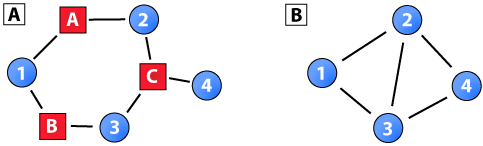
\includegraphics[scale=0.5]{img/1.5_ProyeccionBipartitaClustering.png}
\par\bigskip
\small Fuente: \url{https://toreopsahl.com/tnet/two-mode-networks/clustering/}.
\end{minipage}\bigskip
\begin{description}
    \setlength\itemsep{0em}
    \item[Caso 1 (ilustrado por el evento C y los actores 2, 3 y 4):] Implica que si tres o más actores están relacionados a un mismo evento, son proyectados en un clique cuyo orden es igual al grado simple del evento en el que coparticiparon. 
    Ya que sus relaciones ocurren en un mismo contexto, se puede suponer que cada actor afiliado mantiene un compromiso inmediato con los otros, asegurando una transitividad perfecta. 
    
    \item[Caso 2 (ilustrado por los eventos A, B y C y actores 1, 2, y 3):] 
    En términos de relaciones transitivas, este tipo de ciclos (de longitud 6) también determinan si ``el aliado de mi aliado ha protestado junto a mí''. 
    No obstante, la interpretación es más sutil que en el caso anterior, ya que no involucra una afiliación simultánea; sino que depende de la existencia de al menos un evento que relacione a los actores aliados de otros, con los que se establecieron coaliciones en algún momento. 
    Así, la ecuación \ref{eq:clustering_bipartito_ponderado} es ajustada por \citet{2013_Opsahl_BipartiteCluster} como:
    \vspace{-0.5em}
    \begin{equation}\label{eq:clustering_bipartito_ponderado_opsahl}
	C_{\omega_B} = 
	\frac{ \textbf{valor total de 6-ciclos}}{\textbf{valor total de caminos } P^{4}} 
	= \frac{ \sum_{\tau_{ \bigcirc }} \omega_B}{ \sum_{\tau} \omega_B},
    \end{equation}
    cuyos ``valores totales'' también son calculados a partir de los pesos de las aristas, como en la ecuación \ref{eq:clustering_ponderado}. 
\end{description}


De forma consistente con otros índices, tanto el coeficiente de la ecuación \ref{eq:clustering_bipartito_ponderado}, como el de la  ecuación \ref{eq:clustering_bipartito_ponderado_opsahl} son acotados entre cero y uno, resultando iguales a uno en un grafo bipartito completo. 
Opcionalmente, coeficientes locales de estos índices (centrados en un vértice $i$) pueden ser calculados y comparados entre las clases de una red bimodal o entre una clase y su proyección en una red unimodal. 




% BEGIN         SECCIÓN 1.3.5     HOMOFILIA                                                                        .
\subsection{Homofilia}
\label{subsec:Homofilia}
La \emph{homofilia} o \emph{mezcla selectiva} en redes sociales sugiere que diversos actores mantienen ``una fuerte tendencia a asociarse con otros a los que perciben como similares a ellos de alguna manera''\footnote{
    En oposición a este concepto existen redes donde se ha detectado una fuerte tendencia opuesta (nodos disimilares tienen una mayor probabilidad de relacionarse). 
    Sin embargo, en redes sociales de colaboración el patrón más común es dado por homofilia, de modo que sólo referimos este caso; no obstante, la probabilidad de que vértices opuestos sean relacionados puede calcularse a través de los mismos índices referidos en esta subsección (en el caso de conectividad y atributos). 
} \citep[384]{2010_Newman_Networks}. 
El grado de homofilia presente en una red unimodal\footnote{
    Descartamos la detección de homofilia en redes multimodales, ya que resulta más intuitiva su medición a través de relaciones directas entre vértices del mismo tipo, aún cuando estas hayan sido proyectadas por medio de relaciones indirectas. 
} 
puede estar basado en atributos categóricos (por ejemplo, sexo, grado de estudios o lugar de origen), valores escalares (edad e ingresos entre otros) o medidas relacionales (principalmente grado simple y ponderado). 



En este trabajo nos centramos en tres casos: 
(i) \emph{homofilia conducida por atributos categóricos}, lo cual nos permitiría detectar el nivel de flexibilidad en coaliciones de tipo intersectorial e interregional, entre otros; 
(ii) \emph{homofilia por conectividad}, de modo que se compruebe si actores con un alta semejanza de actividades locales tienden a colaborar más entre sí; 
y (iii) \emph{homofilia por monopolización de relaciones} que podría revelar un elevado control, ejercido por pequeños grupos de actores bien conectados a otros (y especialmente entre sí) sobre la dinámica en la red de colaboración ---de ahí la denominación sobre un \emph{efecto de club rico}---. 
El primer y segundo caso consideran atributos topológicos y de fortaleza (aplicables a redes simples y ponderadas, respectivamente) mientras que el último caso es aplicable sólo a redes ponderadas; por las características de nuestro problema sólo aplicamos estas medidas a proyecciones unimodales, de colaboración en protestas entre actores colectivos.



\subsubsection{Homofilia por atributos categóricos}
\label{subsubsec:HomofiliaCategorica}

Dado un conjunto de $N$ actores colectivos en una red proyectada simple, relacionados por su coparticipación en eventos de protesta (de acuerdo a la sección \ref{subsec:redesBipartitas}), se considera que cada actor puede formar parte de un \emph{sector}, por los objetivos propuestos a los que se les ha podido vincular; o bien, pueden ser caracterizados por el alcance regional sobre el que extienden sus actividades u otros datos covariables ---ver sección \ref{sec:DatosOMS}---. 
De acuerdo a \citet{2010_Newman_Networks}, para sugerir que dicha red colaborativa tiene un alto índice de homofilia bajo cierto atributo, se puede comprobar si una fracción significativa de las aristas en la red son incidentes a vértices en una misma categoría. 

Sin embargo, no basta con que exista una gran cantidad de relaciones que cumplan dicha característica; para enunciar que existe una homofilia significativa en la red dada cierta categorización, se debe comprobar también que la proporción de relaciones entre vértices con una misma característica es mayor que aquella que podríamos esperar debido al azar. 
De este modo, es común que se genere un índice único que calcule la diferencia entre homofilia aleatoria y empírica. 
Sólo cuando esta última sea mayor a la primera podríamos tener cierta confianza en que las relaciones entre actores están fuertemente correlacionadas con cierta característica relevante.

De acuerdo a \citet{2010_Newman_Networks}, para calcular la proporción de aristas entre vértices del mismo tipo (es decir, la homofilia empírica) se puede recurrir a un conteo simple. 
Considerando a $c_{i}$ como la clase a la que pertenece un vértice $i$, se calcula: 
\begin{equation}\label{homofilia_empirica}
    \frac{1}{2M} \sum_{i, j \text{ } \epsilon \text{ } V(G)} A_{ij} \delta(c_{i},c_{j}),
\end{equation} 
donde el factor de $1/2$ evita que los finales de cada arista se cuenten doble, $1/M$ genera una medida proporciona a todas las aristas en la red, $A_{ij}$ considera un elemento de la matriz de adyacencia dicotómica, y la función $\delta(c_{i},c_{j})$ será igual a uno si las clases de los vértices $i$ y $j$ son iguales y cero en otro caso. 

Por otra parte, para obtener la proporción de aristas entre vértices del mismo tipo esperados al azar, se debe preservar ciertos elementos topológicos de la red simple que se está analizando. 
Así, ya que existen $2 \times M$ vértices adyacentes a toda arista en la red, la probabilidad de que \emph{una arista cualquiera} sea adyacente a un vértice $j$ será igual a $k_{j}/2M$, donde $k_{j}$ es el grado simple de $j$. 
Y el número esperado de aristas entre los vértices $i$ y $j$ será $k_{i}k_{j}/2M$. 
Consecuentemente, la proporción de aristas entre vértices del mismo tipo esperados al azar típicamente es calculada como:
\begin{equation}\label{homofilia_aleatoria}
    \frac{1}{2M} \sum_{i, j \text{ } \epsilon \text{ } V(G)} \frac{k_{i}k_{j}}{2M} \delta(c_{i},c_{j}).
\end{equation} 

Restando las ecuaciones \ref{homofilia_empirica} y \ref{homofilia_aleatoria}, se obtiene la diferencia entre la proporción de aristas por homofilia empírica y aleatoria, nombrada \emph{modularidad}: 
\begin{equation}\label{modularidad}
    Q = \frac{1}{2M} \sum_{i, j \text{ } \epsilon \text{ } V(G)} \left(A_{ij} - \frac{k_{i}k_{j}}{2M} \right) \delta(c_{i},c_{j}).
\end{equation} 

Esta medida (y algunas de sus variantes\footnote{
    Por ejemplo, una medida de modularidad ponderada podría ser establecida al sustituir en la ecuación \ref{modularidad}: 
    (i) el producto del grado simple $k_{i}k_{j}$ por aquel asociado a la fortaleza de los vértices $s_{i}s_{j}$; 
    y (ii) el factor $1/M$ por el inverso de la suma de los pesos en la matriz de adyacencia $1/W$; cada elemento $A_{ij}$ a su vez implicaría el peso de una relación y no sólo un marcador binario de su ocurrencia. 
    Una variante en una red bipartita ponderada es presentada en la ecuación \ref{modularidad_bipartita}; de forma similar, la homofilia empírica podría ser calculada de forma análoga independientemente en una red unimodal ponderada. 
}) aparece en distintas aplicaciones en el análisis de redes ---sobre todo en la optimización de detección de comunidades, como se verá en la sección \ref{subsec:Comunidades}---. 
Ya que los resultados de las ecuaciones \ref{homofilia_aleatoria} y \ref{homofilia_empirica} están entre cero y uno, $Q$ será estrictamente menor a uno. 

Usualmente basta que la modularidad sea positiva para proponer homofilia en las relaciones formadas\footnote{
    O valores negativos para suponer que existen una mayor cantidad de relaciones entre vértices de diferentes características de la que se esperaría aleatoriamente.
}. 
Sin embargo, como hemos mencionado en la sección \ref{subsec:redesBipartitas}, resulta problemático asumir independencia en las aristas pertenecientes a una red proyectada ---como lo hace el modelo nulo de la ecuación \ref{homofilia_aleatoria}---, ya que sus relaciones son determinadas a partir de subconjuntos de vértices, incidentes a un vértice de la clase opuesta en la red bipartita original. 
Es por ello, que en lugar de utilizar estas últimas dos ecuaciones, se recurre al cálculo de la ecuación \ref{homofilia_empirica} en múltiples \emph{redes bipartitas aleatorias proyectadas}, que establecen sendos puntos de referencia que permiten comprobar la relevancia de la homofilia empírica calculada ---ver sección \ref{sec:Redes_aleatorias_bipartitas}---. 
La comparación entre homofilia simple y ponderada puede ser informativa, aunque no es común que ésta última sea calculada. 




\subsubsection{Homofilia por conectividad}
\label{subsec:HomofilidadConectividad}

Para comprobar si actores con una actividad parecida en un ámbito local se relacionan entre sí, es posible utilizar una gran variedad de índices\footnote{
    Entre ellos, un índice general parecido al de la ecuación \ref{modularidad}, donde se corrobore la coincidencia en el grado (o fortaleza) entre cada par de colaboradores. 
}. 
En nuestro caso, ya que pretendemos aproximar la correlación selectiva entre la conectividad de actores colaborativos, utilizamos el grado promedio de los $N(i)$ \emph{vértices adyacentes} a $i$, calculado en una red simple como: 
\begin{equation}\label{homofilia_k}
    k_{nn , i} = \frac{1}{k_{i}} \sum_{j \text{ } \epsilon \text{ } N(i)} k_{j}.
\end{equation} 
De modo que (si existe de una fuerte correlación de conectividad entre colaboradores) el grado simple de $i$ y todos sus vecinos será aproximadamente el mismo; es decir, $k_{nn , i} \approx k_i$ para todo $i$. 
A su vez, según \citet{2004_Barrat_ComplexNetworks}, es posible sintetizar estas medidas en función de vértices con el mismo grado, de modo que se represente:
\begin{equation}\label{knn}
    k_{nn}(k) = \sum_{k'}k'P(k'|k),
\end{equation} 
donde $P(k'|k)$ es la probabilidad condicional de que un vértice con grado $k$ esté conectado a un vértice de grado $k'$. 
Esta medida es conocida como la \emph{conectividad promedio de los vértices más cercanos}, para vértices con conectividad $k$. 
Sólo si $k_{nn}(k)$ es una función creciente de $k$ se podrá suponer la presencia de homofilia simple en la red. 


Por otro lado, en el caso de una red ponderada, \citet{2004_Barrat_ComplexNetworks} proponen el siguiente cálculo, análogo a la ecuación \ref{homofilia_k}, para medir \emph{la afinidad efectiva de un actor para conectarse con vecinos de alto o bajo grado}, de acuerdo a la magnitud de sus interacciones registradas: 
\begin{equation}\label{homofilia_kw}
    k^{w}_{nn , i} = \frac{1}{s_{i}} \sum_{j \text{ } \epsilon \text{ } N(i)} w_{ij}k_{j}.
\end{equation} 
De manera que si $k^{w}_{nn , i} > k_{nn , i}$ las aristas con mayor peso conectarán a los vecinos de mayor grado\footnote{
    Y, de forma opuesta, si $k^{w}_{nn , i} < k_{nn , i}$, las aristas con menor peso conectarán a los vecinos de mayor grado.
}. 
Así mismo, el comportamiento de la función $k^{w}_{nn}(k)$ ---análoga a la ecuación \ref{knn}--- registra una aproximación sobre la propiedad de homofilia, teniendo en cuenta las interacciones entre los actores en una estructura social.





\subsubsection{El efecto del club rico}
\label{subsec:ClubRico}

La homofilia basada en las propiedades estructurales de una red tiene una interpretación crucial en redes sociales, donde se ha denominado \emph{efecto del club rico} a la existencia de un grupo selecto de vértices, que comparten y controlan la mayoría de los recursos en la red. 
Esta hipótesis ofrece una analogía al principio empírico de Pareto\footnote{
    Que supone que sólo una minoría (20\%) de elementos es responsable de la gran mayoría (80\%) de los resultados observados. 
} 
desde un punto de vista relacional. 

Para ponerla a prueba en una \emph{red proyectada ponderada}, se puede corroborar si vértices altamente conectados tienen relaciones más fuertes entre ellos de lo esperado al azar. 
Con este fin, \citet{2008_Ophsal_RichClub} proponen asignar un \emph{ranking} a cada vértice en la red por medio de un \emph{parámetro de riqueza} $r$, el cual es determinado ---en este caso particular--- por su fortaleza $s_{i}$. 

\hspace{-1.5em}\begin{minipage}{\linewidth}
\centering
\captionof{figure}{Relaciones entre los vértices más prominentes (A) y relaciones con mayor peso en una red (B)} \label{1.6_ClubRico}
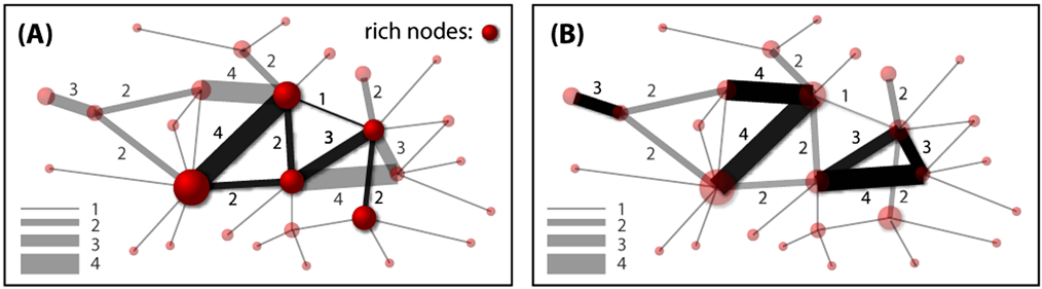
\includegraphics[scale=.4]{img/1.6_ClubRico.png}
\par\bigskip
\small Fuente: \citep[2]{2008_Ophsal_RichClub}
\end{minipage}\bigskip


``Para cada valor de $r$ se selecciona el grupo (o club) de vértices cuya riqueza es mayor a $r$. Obteniendo una serie de clubes cada vez más selectivos'' \citep[1]{2008_Ophsal_RichClub}. 
En cada club se obtiene el número de aristas que conectan a sus miembros ($M>r$) así como la suma de sus ponderaciones ($W>r$). 
Finalmente, se calcula la relación entre $W>r$ ---figura \ref{1.6_ClubRico} (A)--- y la suma total de ponderaciones que los vértices seleccionados podrían tener si estuvieran relacionados a través de las aristas con mayor peso de la red ---figura \ref{1.6_ClubRico} (B)---.
\begin{equation}\label{pesos_compartidos_ricos}
    \phi^{w}(r) = \frac{W_{> r}}{\sum_{l=1}^{M_{> r}} w_{l}^{ranking}},
\end{equation} 
donde $w_{l}^{ranking} \geq w_{l+1}^{ranking}$ con $l = 1,2,...,M$ son los pesos rankeados de las aristas de la red y $M$ es su número. 
De tal modo que $0 < \phi^{w}(r) \leq 1$. 



No obstante, un alto valor de $\phi^{w}(r)$ no es suficiente por sí mismo para asegurar un efecto de club rico. 
Como antes, este valor es comparado con un modelo nulo. 
Lo cual nos permite asegurar que existe un efecto mayor al que se podría esperar debido al azar. 
Al respecto \citet{2008_Ophsal_RichClub} sugiere el siguiente cociente: 
\begin{equation}\label{eq:club_rico}
    \rho^{w}(r) = \frac{\phi^{w}(r)}{\phi^{w}_{\text{nulo}}(r)}.
\end{equation} 
Donde si $\rho^{w}(r)$ es mayor que uno ---es decir, $\phi^{w}(r) > \phi^{w}_{\text{nulo}}(r)$--- se obtendría evidencia a favor de la hipótesis del efecto del club rico (en cierto subconjunto de vértices); de forma opuesta, valores menores a uno exhibirán un efecto inverso (implicando, por ejemplo, competitividad de recursos entre los vértices posicionados de forma superior). 


Para un adecuado punto de referencia, consideraremos en este trabajo\footnote{
    Según las recomendaciones hechas por Ophsal en \url{https://toreopsahl.com/tnet/two-mode-networks/weighted-rich-club-effect/}.
} que $\phi^{w}_{\text{nulo}}(r)$ será el promedio del cociente en la ecuación \ref{pesos_compartidos_ricos}, calculado en múltiples redes aleatorias bipartitas ---ver sección \ref{sec:Redes_aleatorias_bipartitas}--- proyectadas bajo el mismo método que la red ponderada analizada. 





\subsection{Redes aleatorias bipartitas}
\label{sec:Redes_aleatorias_bipartitas}

El objetivo que nos motiva para utilizar redes aleatorias como modelo nulo es el mismo que en el caso de modularidad: contrastar cierta información obtenida en redes empíricas bipartitas (o sus proyecciones) a fin de determinar su relevancia. 
Esta comparación puede resultar útil no sólo para comprobar una hipótesis de homofilia en redes proyectadas (como se planteó en la sección anterior), sino también para evaluar otras medidas (en nuestro caso, los coeficientes de clustering y reforzamiento). 


Sostenemos que esta es una estrategia adecuada debido a que cada simulación de una red aleatoria puede producir topologías diferentes. 
De modo que es posible especificar intervalos de confianza ---por ejemplo, del 95\%---, al simular cientos o miles de redes aleatorias en las que se hayan obtenido valores análogos a aquellos que se contrastan. 

Para que este modelo nulo sea razonable, se considera que las redes simuladas deberán preservar ciertas características de la red original analizada. 
A pesar de que en redes unimodales \citet{2002_Barabasi_MechanicsOfComplexNetworks} refieren diversos modelos que preservan ciertas características empíricas, existen pocas alternativas para redes bipartitas. 
Basándonos en el paquete \emph{tnet} desarrollado por \citet{2015_Ophsal_tnet}, consideraremos dos opciones:
\begin{description}
    \item[Modelo clásico.] Se mantiene el orden en cada clase $n_{1}$ y $n_{2}$, así como el número de  aristas $M$ de la red original; no obstante, cada par de vértices en diferentes clases tendrá una probabilidad uniforme de ser relacionado. Una desventaja de esta opción es que la distribución de grado dada por esta técnica (típicamente uniforme o poisson en redes unimodales) es diferente a la que se observa en redes empíricas, por lo que no se recomienda su uso cuando cierta información empírica sea dependiente de tal distribución. Adicionalmente, es posible crear relaciones ponderadas, las cuales se eligen aleatoriamente (también con probabilidad uniforme) de un vector con pesos definidos. 
    \item[Reordenamiento de aristas.] Además de las características anteriores, esta alternativa preserva la distribución de grado de la red original (y de fortaleza en el caso de redes bipartitas ponderadas), no obstante se reordenan las relaciones existentes. 
\end{description} 


Utilizaremos la primer opción para evaluar los coeficientes de clustering y reforzamiento (presentados en la sección \ref{sec:CoeficienteClustering}), ya que supone una comparación razonable y resulta más eficiente en términos computacionales en nuestro caso. 
Por su parte, la segunda opción será utilizada como modelo nulo para diagnosticar la relevancia en las medidas de homofilia (guiadas por atributos categóricos), así como para contrastar \nameref{subsec:ClubRico} para diversos subgrupos de vértices. 

Como señalan \citet{2002_Barabasi_MechanicsOfComplexNetworks}, ciertos modelos de redes aleatorias implican valores esperados muy diferentes de aquellas mediciones observadas en redes empíricas, los cuales son dependientes del orden de la red\footnote{
    Por ejemplo, este es el caso en redes simples del coeficiente de clustering global, definido como el promedio de los coeficientes de clustering locales, cuyo valor esperado en un modelo clásico es linealmente decreciente respecto al tamaño de un grafo. 
} u otras características preservadas. 
Por lo que al comparar datos empíricos y aleatorios, se debe tener en cuenta que dicha confrontación sólo se evalúa en términos de las dinámicas particulares que generan ambos tipos de redes. 
Consecuentemente, sólo podríamos afirmar que una observación es relevante dada la suposición de que las relaciones fuesen aleatorias en un sentido específico, según propone cierto modelo. 




\subsection{Equivalencias y similaridades entre vértices}
\label{sec:EquivalenciaYSimilaridad}

Dada una configuración heterogénea de vínculos en una red social, se pueden identificar \emph{posiciones equivalentes} entre subconjuntos de actores, de acuerdo a ciertas condiciones relacionales que las distinga. 
En redes sociales, una aproximación frecuente supone identificar ``una colección de actores que son similares en actividad social, vínculos o interacciones, con respecto a actores en otras posiciones'' \citep[348]{1994_Wasserman_SNA}. 


Al respecto, \citet{1994_Wasserman_SNA} especifican como pasos necesarios para realizar un \emph{análisis posicional}: 
\begin{description}
    \item[1. Establecer una definición formal de equivalencia.] 
    Según \citet{2010_Newman_Networks}, existen dos enfoques comunes para construir medidas de similaridad, que permiten hallar actores con posiciones análogas: 
    \emph{equivalencia estructural} y \emph{equivalencia regular}. 
    Idealmente, dos vértices serán equivalentes \emph{estructuralmente} si comparten todos sus vértices adyacentes, y serán equivalentes \emph{regularmente} si tanto ellos como sus vértices adyacentes mantienen patrones relacionales indistinguibles en la red (considerando una o más posiciones globales), como se muestra en la figura \ref{1.7_equivalencia_str_reg}. 
    Ya que la equivalencia regular implica condiciones menos restrictivas, fijadas más allá de un ambiente local, se presume que si dos vértices son estructuralmente equivalentes también serán regularmente equivalentes\footnote{
	\citet{1994_Wasserman_SNA} refieren a la \emph{equivalencia automórfica} como un tercer enfoque aplicable en redes simples. 
	De modo que ``dos actores son equivalentes automorficamente si y sólo si existe un automorfismo, $\tau$, que mapee uno de los actores al otro'' \citep[470]{1994_Wasserman_SNA}. 
	Esta es una medida más restrictiva que la equivalencia regular y menos que la equivalencia estructural, no la utilizamos en este trabajo al tratarse de un enfoque intermedio y debido a que sus medidas de similaridad han sido poco estudiadas. 
    }. 
    
    
\begin{minipage}{\linewidth}
    \centering
    \captionof{figure}{Equivalencia estructural y equivalencia regular.} \label{1.7_equivalencia_str_reg}
    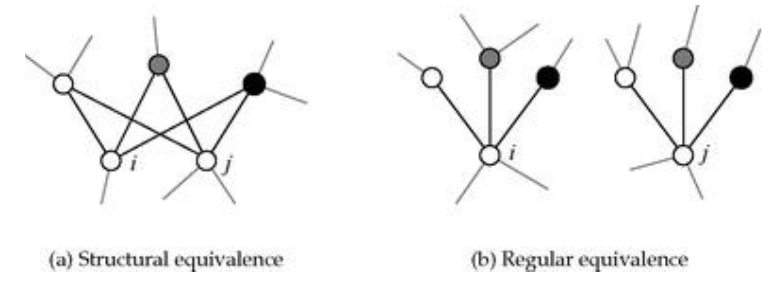
\includegraphics[scale=.4]{img/1.7_equivalencia_str_reg.png}
    \par\bigskip
    \small Fuente: \citep[214]{2010_Newman_Networks}. 
\end{minipage}\medskip

    \item[2. Establecer una medida de \emph{similaridad} que calcule el nivel de ajuste a la definición dada.] 
    Con base en las definiciones formales de equivalencias (y ya que en la práctica resulta sumamente difícil que se cumplan sus condiciones) se han sugerido medidas de similaridad que calculan un nivel de ajuste relativo. 
    
    Tomando la idea de equivalencia estructural, diversas medidas de similaridad han proporcionado buenos resultados para distintos tipos de redes y han sido ampliamente utilizadas; 
    de ellas elegimos la \emph{distancia euclidiana}, que en realidad es una medida de disimilitud, pero cuyos valores se ajustan adecuadamente a una definición formal de equivalencia estructural, es ampliamente utilizada en el análisis de redes y tiene una fácil interpretación al comparar pares de vértices. 
    
    Por otra parte, el concepto de equivalencia regular resulta mucho más conflictivo de acuerdo a \citet{1994_Wasserman_SNA}, ya que (a diferencia de la equivalencia estructural) pueden existir múltiples particiones de actores ---derivadas de distintas proposiciones--- que satisfagan la definición. 
    Al respecto, \citet{2006_Newman_Similarity} refieren dos tipos de algoritmos recursivos empleados para su determinación: 
    (i) aquellos que buscan una correspondencia óptima entre los vértices adyacentes a pares de actores ---sin tener un razonamiento teórico transparente---; 
    o bien (ii) algunos que proponen una optimización respecto a matrices ideales propuestas ---cuya convergencia resulta problemática---. 
    En su lugar, presentan una alternativa derivada de la \nameref{sec:Centralidad_Katz} (la cual hemos adoptado en este trabajo), que resulta aplicable a redes unimodales simples, puede ser considerada una generalización de otras medidas de equivalencia estructural en redes simples y permite incorporar una matriz de similaridad calculada a priori (donde podríamos emplear similaridades basadas en más de un atributo categórico entre actores). 
    
    
    \item[3. Generar una representación de las equivalencias.] 
    El análisis general de las similaridades se puede hacer directamente por medio de las matrices calculadas; no obstante, no resulta fácil deducir patrones generales en redes con una gran cantidad de vértices. 
    En su lugar, es preferible obtener una representación agrupada, la cual puede ser ajustada a un modelo continuo (por ejemplo, a través de un \emph{escalamiento multidimensional}\footnote{
	Donde las medidas de disimilitud (complementarias a las similaridades calculadas) son interpretadas como distancias y representadas espacialmente en una, dos o más dimensiones. 
	Conforme se incrementa el número de dimensiones, habrá un mayor ajuste en relación a las disimilitudes originales; sin embargo, dimensiones mayores a dos son difíciles de interpretar y dimensiones mayores a tres no pueden ser presentadas visualmente. 
	Por lo que es común que se emplee un espacio bidimensional para representar diferencias relativas, comprometiendo su bondad de ajuste para para redes de gran tamaño, cuyos patrones de relación no sean reiterativos.
    }) o discreto (por una partición en \emph{clases de equivalencia} ---también referidas como \emph{bloques}---). 
    
    
    
    En este trabajo nos decantamos por la segunda opción, dado que una partición discreta también implica un método de detección de comunidades ---ver sección \ref{subsec:Comunidades}---. 
    Donde, como en otras aproximaciones, el principal objetivo es la agrupación de subconjuntos de vértices que potencialmente revelen propiedades generales de una red; adicionalmente, también es común que se aglutinen las relaciones originales entre los miembros de cada clase en una red más pequeña, denominada \emph{modelo de bloques} ---de forma similar a como se muestra en la figura \ref{1.9_infomap} (d)---. 
    De esta forma, cada \emph{bloque} (incorporado o no a una red agregada) considera vértices cuyas posiciones sociales resultan (hasta cierto punto) equivalentes, de acuerdo a un umbral de similaridad fijado. 
    El algoritmo que utilizamos para hacer esta partición es el \emph{clustering jerárquico} ---reseñado en la sección \ref{sec:ClasesEquivalentes}---, que supone un método aglomerativo, el cual  realiza $N-1$ particiones sucesivas bajo distintos niveles de ajuste, hasta que todos los vértices de una red forman parte de una misma agrupación. 
    Como en otros métodos de detección de comunidades, únicamente seleccionamos una partición particular (es decir, que no creamos una red agregada) con el evitar una síntesis demasiado condensada, que implique una alta pérdida de información. 
    
    
    \item[4. Evaluar qué tan adecuada es dicha representación.] 
    Ya que es inusual que se produzcan equivalencias perfectas, esto supone en nuestro caso debatir la relevancia de las similaridades obtenidas, la idoneidad de su manipulación a través del método de clustering elegido, así como la evaluación de los grupos obtenidos con base en su correspondencia relacional y teórica. 
    Una vez que seleccionamos una partición en grupos, utilizamos al \emph{índice de Dunn} ---ecuación \ref{indice_Dunn}--- para comprobar su pertinencia cuantitativa. 
\end{description}

En seguida referimos sendas definiciones formales de equivalencias estructural y regular señaladas por \citet{1994_Wasserman_SNA}\footnote{
    Adecuadas a nuestra notación, considerando además un solo conjunto de relaciones $E(G)$, ponderado y no dirigido.
}; así como su transición hacia las similaridades empleadas en este trabajo. 


\subsubsection{Equivalencia estructural}
\label{sec:EquivalenciaEstructural}


\begin{definition}[Equivalencia estructural]
\label{EquivalenciaEstructural}
    Dos vértices $i, j \ \epsilon \ V(G)$ son estructuralmente equivalentes si y solo si $\{i,k\}, \{j,k\} \ \epsilon \ E(G) $ con $w_{jk} = w_{ki} \ \forall \ k \ \epsilon \ V(G)$ adyacente a $i$ y $j$ respectivamente, tal que $k \neq i,j$.
\end{definition}

Según esta definición ---proveniente de la sociología--- actores estructuralmente equivalentes deberían tener relaciones idénticas (incluyendo pesos asociados) con un mismo subconjunto de actores; por lo tanto, aquellos actores estructuralmente equivalentes resultan \emph{sustituibles} en la red. 

Calculamos la (di)similaridad respecto a este tipo de equivalencia a través de la \emph{distancia euclidiana}\footnote{
    También conocida en redes simples como ``hamming distance'', que en teoría de la información refiere el mínimo número de sustituciones requeridas para reemplazar una cadena con otra. 
    Una medida de similaridad puede ser obtenida por su complemento; es decir, $1-d_{ij}$.
    A pesar de que la distancia euclidiana es utilizada principalmente en redes simples, la ecuación \ref{distancia_euclidiana} es una medida de disimilaridad adecuada en una red ponderada. 
}, 
que se define como las ponderaciones normalizadas que difieren hacia vértices comunes entre $i$ y $j$. 
Es decir, que el numerador de la fracción resultante indica la diferencia de pesos en las relaciones que conectan a $i$ con un mismo subconjunto de vértices adyacentes a $j$ (y viceversa), mientras que el denominador acota su valor en relación a la suma de sus fortalezas al cuadrado\footnote{
    Es decir, el máximo valor teórico, cuando no hay ningún vértice en común.
}: 

\begin{definition}[Distancia euclidiana]
\label{distancia_euclidiana}
    \begin{equation}
	d_{ij} = \frac{\sum_{k} (A_{ik}-A_{jk})^2}{s_{i}^2+s_{j}^2}. 
    \end{equation} 
\end{definition}

Como sugiere la definición \ref{EquivalenciaEstructural}, \emph{vértices estructuralmente equivalentes} tendrán ponderaciones y relaciones idénticas con un mismo subconjunto de unidades sociales (obteniendo una distancia igual a cero); por otro lado, si un par de vértices no sostienen al menos una relación en común con un tercero, entonces no habrá ninguna similaridad estructural entre ellos y $d_{ij}$ será igual a uno. 
En una red social de coalición, como aquella que abordamos en la sección \ref{sec:RedProyectada_coparticipación}, una menor distancia euclidiana será dada por una gran coincidencia en el número y fortaleza de relaciones con un mismo grupo de colaboradores adyacentes, en relación al total de coparticipaciones de un par de actores. 




\subsubsection{Equivalencia regular}
\label{sec:EquivalenciaRegular}

\begin{definition}[Equivalencia regular]
\label{EquivalenciaRegular}
    Dos vértices $i, j \ \epsilon \ V(G)$ son regularmente equivalentes si $\forall \ k \ \epsilon \ V(G)$ con $\{i,k\} \ \epsilon \ E(G) $ existe algún $  l  \  \epsilon \ V(G)$ tal que  $\{j,l\} \ \epsilon \ E(G)$, donde $k$ es regularmente equivalente a $l$.
\end{definition}

Esta definición propone que aún vértices no adyacentes pueden tener posiciones equivalente si (por las unidades sociales con las que se relacionan) son ubicados en un entorno global semejante; una aproximación intuitiva ---asociable con el desempeño de \emph{roles sociales}--- es descrita por \citet{1994_Wasserman_SNA}:

\begin{center}
    \begin{minipage}{0.9\linewidth}
        {\setlength{\parindent}{12pt}\small
         Brevemente, los actores que son regularmente equivalentes tienen lazos idénticos de y hacia actores equivalentes. 
         Por ejemplo, los bullies en un vecindario ocupan la misma posición social, aunque en diferentes vecindarios, porque golpean a algun(os) niño(s) y son regañados por algun(os) padre(s) iracundo(s), pero no necesariamente golpean al (o los) mismo(s) niño(s) ni son regañados por el (o los) mismo(s) padre(s).
         \normalsize \citep[474]{1994_Wasserman_SNA}.
        }
    \end{minipage}
\end{center}



Debido a la dificultad para distinguir diferentes condiciones sociales entre vértices dispersos únicamente a partir de una estructura relacional, ``las  medidas cuantitativas de equivalencia regular están menos desarrolladas que las medidas de equivalencia estructural'' \citep[221]{2010_Newman_Networks}; por lo que sólo se ofrecen diferentes aproximaciones (con deficiencias propias) que pretenden crear clases de equivalencia distintivas. 


Ya que en la definición \ref{EquivalenciaRegular}, la equivalencia regular se define recursivamente (es decir, en términos de los vértices adyacentes a un par de unidades sociales, cuya equivalencia se define de la misma manera); \citet{2010_Newman_Networks} sugiere que una medida de similaridad $\sigma_{ij}$ entre dos vértices $i,j$ podría ser obtenida a partir de la \emph{suma ponderada de similaridades a priori} $\sigma_{kl}$, entre los vértices $k$ (adyacentes a $i$) y $l$ (adyacentes a $j$):
\begin{equation}\label{eq:aprox_sim}
    \sigma_{ij} = \alpha \sum_{\{\text{ }k \text{ }|\text{ } ik \text{ } \epsilon \text{ } E(g)\}}\sum_{\{\text{ }l\text{ } | \text{ }jl \text{ } \epsilon \text{ } E(g)\}} A_{ik}A_{jl}\sigma_{kl} + \delta_{ij},
\end{equation}
donde $\alpha$ es una ponderación que asegura la convergencia de valores si $\sigma_{kl}$ se define recursivamente, y el término $\delta_{ij}$ será igual a uno si $i=j$ (ya que es obvio que un vértice es equivalente a sí mismo) y cero en otro caso. 


No obstante, \citet{2010_Newman_Networks} también señala que el cálculo iterativo de la ecuación \ref{eq:aprox_sim} define la similaridad sólo en términos de caminos de longitud par, lo cual restringe la determinación de su posicionamiento global. 
Para considerar caminos de cualquier longitud, \citet{2006_Newman_Similarity} simplifican el sentido original de la definición \ref{EquivalenciaRegular} y suponen la presencia de homofilia en la red (es decir, que las relaciones directas por sí mismas indican un alto nivel de similaridad entre el grado de los vértices que conectan). 
De modo que, como se muestra en la figura \ref{1.8_simKatz}\footnote{
    Donde las líneas punteadas representan similaridades y las sólidas son interpretadas como aristas. 
}, 
proponen que: \emph{si los vértices $i$ y $j$ son regularmente similares, entonces existe un vértice $k$ adyacente a $i$ que a su vez es similar a $j$}. 


\begin{minipage}{\linewidth}
\centering
\captionof{figure}{Similaridad regular (de Katz) entre vértices \{$i$,$j$\} y \{$k$,$j$\}.} \label{1.8_simKatz}
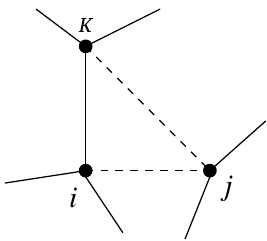
\includegraphics[scale=0.5]{img/1.8_simKatz.png}
\par\bigskip
\small Fuente: \citep[2]{2006_Newman_Similarity}.
\end{minipage}\bigskip


En nuestra red de coaliciones de eventos de protestas, esto equivale a argumentar que dos actores colectivos son similares entre sí, si ambos se relacionan de forma parecida respecto al otro y sus colaboradores (es decir, que tales organizaciones coparticipativas crean coaliciones que los sitúan en una posición relativa semejante dentro de una estructura social). 
Dado que consideramos relaciones recíprocas, altos niveles de similaridad serán definidos idealmente para subgrupos de actores, no necesariamente adyacentes. 



A partir de esta diferenciación, y de conformidad con el razonamiento expuesto para la ecuación \ref{eq:aprox_sim}, podemos definir una expresión análoga en $t$ iteraciones: 
\begin{equation}\label{eq:similaridad_regular}
    \sigma_{ij}(t) = \alpha \sum_{k} A_{ik} \sigma_{kj}(t-1) + \delta_{ij},
\end{equation}
donde $\alpha$ es un factor de atenuación que penaliza relaciones indirectas (de acuerdo a su longitud)\footnote{
    Y  también asegura la convergencia de valores al calcular recursivamente $\sigma_{kj}$, dado que esta es una ecuación de vector propio. 
    Como para la \nameref{sec:Centralidad_vector_propio} o la \nameref{sec:Centralidad_Katz} ---si tomamos en consideración la ecuación \ref{eq:similaridadKatz}--- se debe cumplir que $0 < \alpha < 1/\lambda_l$; donde $\lambda_l$ es el mayor vector propio de la matriz de adyacencia. 
    No obstante, como señalan \citet{2018_Duricic_RegularEquivalence} cuando esta similaridad se calcula de forma iterativa, se puede detener la recursividad en las ecuaciones \ref{eq:similaridad_regular} o \ref{eq:similaridad_regular_normalizada} en $t = t_{max}+1$, de modo que se evite la divergencia de valores y se limite la propagación de similaridades en la red, a través caminos de longitud menor e igual a $t_{max}$; en esos casos se podría utilizar cualquier valor de $\alpha$ entre cero y uno. 
}. 
En notación matricial, podemos reescribir la expresión, como:
\begin{equation}\label{eq:similaridad_regular_matrix}
    \mathbf{\sigma}^{(t)} = 
    \alpha \mathbf{A}\mathbf{\sigma}^{(t-1)} + \mathbf{I}.
\end{equation}

Considerando una matriz de similaridad inicial $\mathbf{\sigma}^{(0)}$ cuyas entradas sean iguales a cero; 
en la primer iteración obtendríamos $\mathbf{\sigma}^{(1)}= I$, lo cual refleja el hecho de que todo vértice es equivalente a sí mismo; 
en la segunda iteración, $\mathbf{\sigma}^{(2)}= I + \alpha \mathbf{A}$ (es decir, que vértices adyacentes tendrán una similaridad igual a $\alpha$); 
en la tercer iteración $\mathbf{\sigma}^{(3)}= I + \alpha \mathbf{A} + \alpha^{2} \mathbf{A}^{2}$ (una similaridad igual a $\alpha^{2}$ es asociada a vértices conectados por medio de un camino de longitud dos); y así sucesivamente. 
En el límite (para un gran número de iteraciones) y por la serie geométrica tenemos:
\begin{equation}\label{eq:similaridadKatz}
    \mathbf{\sigma} = 
    \sum_{m=0}^{\infty}(\alpha \mathbf{A})^{m} = 
    (\mathbf{I}-\alpha\mathbf{A})^{-1},
\end{equation} 
que es equivalente a la ecuación \ref{eq:centralidad_katz} que define la centralidad de Katz. 
De forma congruente con ella, ``la idea detrás de la similaridad de Katz es que las rutas de cualquier longitud contribuyen al valor de la similitud entre dos vértices en la red, y las rutas más cortas tienen un impacto más fuerte'' \citep[447]{2018_Duricic_RegularEquivalence}. 
Así, cuando existe una acentuada distinción entre posicionamientos en una red, dos vértices serán \emph{similares regularmente} si son adyacentes a los mismos vértices ---es decir, tienen una gran similaridad estructural---, pero también si estos vértices colindantes mantienen patrones de relaciones (principalmente locales, aunque también globales) parecidos. 


Sin embargo, es importante considerar que al ser una similaridad íntimamente relacionada a una medida de centralidad, acarrea algunos problemas: 

\begin{center}
    \begin{minipage}{0.9\linewidth}
        {\setlength{\parindent}{12pt}\small
         Tal como se define, tiende a proporcionar una gran similitud a vértices con alto grado, ya que si un vértice tiene muchos vecinos tiende a aumentar el número de aquellos vecinos que son similares a cualquier otro vértice dado y por lo tanto, aumenta la similitud total de ese vértice. 
         En algunos casos, esto podría ser deseable: tal vez una persona con muchos amigos \emph{debería} considerarse más similar a los demás que la persona con pocos. 
         Sin embargo, en otros casos proporciona un sesgo no deseado a favor de vértices de alto grado. 
         \normalsize \citep[224]{2010_Newman_Networks}.
        }
    \end{minipage}
\end{center}

Para omitir este sesgo, se puede normalizar este valor dividiendo la ecuación \ref{eq:similaridad_regular} por el grado de cada vértice: 
\begin{equation}\label{eq:similaridad_regular_normalizada}
    \sigma_{ij}(t) = \frac{\alpha}{k_{i}}  \sum_{k} A_{ik} \sigma_{kj}(t-1) + \delta_{ij}, 
\end{equation}
en notación matricial, donde $\mathbf{D}$ es la matriz diagonal con elementos $D_{ii}=k_{i}$, y siguiendo el mismo procedimiento de la ecuación \ref{eq:similaridadKatz}: 
\begin{equation}\label{eq:similaridadKatz_ponderada}
    \mathbf{\sigma} = 
    \alpha \mathbf{D}^{-1}\mathbf{A}\mathbf{\sigma} + \mathbf{I} = 
    (\mathbf{I}-\alpha\mathbf{D}^{-1}\mathbf{A})^{-1}. 
\end{equation}
Empero, cada cálculo iterativo de la matriz $\sigma$ implicaría una normalización por filas que rompe la simetría de las relaciones ($\sigma_{ij} \neq \sigma_{ji}$), lo cual resulta contraintuitivo; de modo que cuanto mayor sea el grado de un vértice, mayor será la atenuación que se generará sobre la suma total de similaridades con otros vértices. 
Según \citet{2018_Duricic_RegularEquivalence}, otra normalización por filas (en relación a una norma $l1$, $l2$ o $max$\footnote{
    La norma $l1$ es obtenida por la suma de los valores absolutos en una fila. 
    $l2$ (o norma euclidiana) es calculada como la raíz cuadrada de la suma de valores al cuadrado en una fila. 
    Finalmente, la norma $max$ ---recomendada por \citet{2018_Duricic_RegularEquivalence}--- es igual al máximo valor de una fila. 
}) es pertinente luego de obtener una matriz de similaridad convergente $\mathbf{\sigma}$ ---dada la ecuación \ref{eq:similaridad_regular_normalizada}---; cuando sus valores sean demasiado pequeños ---y por tanto resulten insuficientes para identificar clases de equivalencia---. 



Ya que el cálculo iterativo de las ecuaciones \ref{eq:similaridad_regular} y \ref{eq:similaridad_regular_normalizada} supone la propagación de similaridades por caminos progresivamente mayores, únicamente se podrá establecer cierta similaridad entre los vértices pertenecientes a una misma componente. 
Para modificar este comportamiento e incorporar información adicional que cuantifique semejanzas regulares (vinculables al desempeño de roles sociales) entre vértices, \citet{2010_Newman_Networks} sugiere añadir tales similaridades a priori al último término de estas ecuaciones ---alterando los términos fuera de la diagonal principal en la matriz identidad resultante--- para hacer explícito cierto grado de similaridad regular a priori (basado en información relacional o no) entre cualquier par de vértices. 




\subsection{Comunidades}
\label{subsec:Comunidades}

Los métodos de detección de comunidades son herramientas que simplifican y resaltan aspectos estructurales de una red, los cuales han sido diseñados para identificar subgrupos de vértices fuertemente interconectados que a menudo corresponden a unidades funcionales importantes, esenciales para comprender su organización \citep[3]{2014_Rosvall_CommunityMapEq}. 

Consecuentemente, la noción de \emph{estructura de comunidad} es relacionada a redes cuyos vértices pueden ser divididos en subgrupos o \emph{comunidades} de propiedades distintivas ---\citet{2010_Newman_Networks}---; vinculadas a sus procesos de formación o flujos dinámicos que caracterizan un sistema ---\citet{2009_Rosvall_MapEquation}---. 
Según \citet{2014_Rosvall_CommunityMapEq}, existen tres principales enfoques en los que se basan los algoritmos de detección de comunidades: 
\begin{description}
    \setlength\itemsep{0em}
    \item[Modelos nulos.] Que comparan alguna medida de conectividad entre grupos de vértices, con el valor esperado en un modelo nulo apropiado (por ejemplo, modularidad). De manera que las comunidades se determinan como los subconjuntos de vértices para los cuales existe una mayor conectividad respecto al modelo nulo. 
    \item[Modelos de bloques.] Donde se identifican ``bloques'' de vértices con propiedades comunes. Los miembros de un bloque son estadísticamente equivalentes, en términos de su conectividad a vértices dentro del bloque al que pertenecen, y diferentes respecto a miembros de otros bloques. La estructura latente de bloques es identificada maximizando la probabilidad de observar los datos empíricos. 
    \item[Modelos de flujo.] Operan sobre la dinámica en la red en lugar de su estructura topológica, capturando el flujo entre los elementos de los sistemas reales que representan. De modo que las comunidades se componen de vértices en los que el flujo tiene una gran persistencia una vez que éste ingresa en alguno de sus miembros. 
\end{description}


La mayor parte de los algoritmos derivados de estos modelos consideran particiones discretas no superpuestas, y sólo algunos de ellos permiten la asignación de vértices a más de una comunidad. 
Algunos métodos permiten incorporar información contextual adicional que facilite la identificación de regularidades entre vértices (por ejemplo datos categóricos o similaridades no basadas en la información de la red), mientras que la mayoría sólo se basa en datos relacionales. 
Unas formulaciones requieren de parámetros o técnicas adicionales que determinen (directa o indirectamente) el número de comunidades resultantes, mientras que otras se basan sólo en la estructura de la red para suponer un número óptimo de comunidades. 
Gran parte de estos métodos pueden ser aplicados a diferentes tipos de redes (por ejemplo, a redes ponderadas, dirigidas o multipartitas), mientras que otros algoritmos han sido diseñados específicamente para redes con características distintivas. 
Como señalan \citet{2009_Rosvall_MapEquation}, cada método y parámetros elegidos implican distintas hipótesis sobre una estructura de comunidad, por lo que producen diferentes particiones que enfatizan aspectos singulares de una estructura; de modo que deben ser utilizados de acuerdo al problema abordado y el tipo de información que se desea extraer. 


En esta sección referimos tres algoritmos que pueden ser utilizados de forma amplia para determinar comunidades en redes bipartitas o proyecciones ponderadas. 
Estos son \emph{DIRTLPAwb+}, \emph{Infomap} y \emph{Clustering jerárquico}, los cuales se han elegido ---además de su amplio alcance--- por la diferencia de perspectivas incorporadas o la consistencia de resultados en pruebas preliminares\footnote{
    En redes bipartitas, se han comparado distintas comunidades halladas por los algoritmos \emph{LPAwb+}, \emph{DIRTLPAwb+} y \emph{QuanBiMo}, disponibles en el paquete \emph{bipartite}, de \emph{R}, donde una mayor modularidad y consistencia de particiones fue hallada por medio de \emph{DIRTLPAwb+} ---confirmando los resultados reportados por \citet{2016_Beckett_ComunidadesBipatitas}---. 
    En el caso de redes ponderadas, la elección de \emph{Infomap} está orientada por los principios de flujo interdependiente y teoría de la información en los que se basa el método desarrollado por \citet{2009_Rosvall_MapEquation}. 
    Por último, en el caso del \emph{Clustering jerárquico}, nos ha interesado validar si existe una fuerte regularidad en patrones de conectividad (basadas en equivalencia estructural); y si los \emph{bloques} deducidos por equivalencia regular son relevantes al incorporar (a la similaridad de Katz) semejanzas derivadas de atributos no relacionales, como se ha propuesto en la sección \ref{sec:EquivalenciaYSimilaridad}, permitiendo incorporar \emph{información contextual} que suele ser omitida en otros algoritmos de detección de comunidades.
}. 



\subsubsection{Comunidades en redes bipartitas ponderadas: LPAwb+ y DIRTLPAwb+}
\label{sec:DIRTLPAwb+}

Dado nuestro análisis de redes de coaliciones en eventos de protesta, la identificación de comunidades en redes bipartitas buscará realizar una distinción de formas asociativas fuertemente interconectadas entre dos o más unidades sociales, determinadas por la recurrencia de sus interacciones en protestas. 


Según \citet{2016_Beckett_ComunidadesBipatitas}, actualmente existen pocos algoritmos de detección de comunidades en redes bipartitas. 
Motivo por el cual él mismo modifica el algoritmo \emph{LPAb+}\footnote{
    El cual a su vez, es una modificación del algoritmo \emph{LPAb} (acrónimo de \emph{Label Propagation Algorithm bipartite}), en la que se implementaron mejoras ---replicadas por \citet{2016_Beckett_ComunidadesBipatitas}--- para escapar de un óptimo local, en el que solía quedar atrapado el algoritmo original. 
} 
a fin de lidiar con redes bipartitas ponderadas. 
Los algoritmos resultantes son \emph{LPAwb+} y \emph{DIRTLPAwb+}. 


Su enfoque está dirigido a maximizar una medida de modularidad, como la que se ha presentado en la ecuación \ref{modularidad}. 
Sin embargo (debido a la restricción para crear relaciones entre vértices de la misma clase), se redefine la modularidad a partir de una matriz de afiliación rectangular ponderada $\mathbf{B}$ (introducida en la sección \ref{subsec:redesBipartitas}): 
\begin{equation}\label{modularidad_bipartita}
    Q_{W} = \frac{1}{W} \sum_{i=1}^{n_{1}} \sum_{j=1}^{n_{2}} \left( b_{ij} - \frac{s_{i}s_{j}}{W} \right) \delta(g_{i},h_{j}),
\end{equation} 
donde $b_{ij}$ es la entrada $(i,j)$ de la matriz rectangular ponderada $\mathbf{B}$ de dimensiones $n_{1}\times n_{2}$; $s_{i}$ y $s_{j}$ es la fortaleza (según la ecuación \ref{s_i}\footnote{
    Aunque considerando una matriz de afiliación, $s_{i}$ es calculada como la suma marginal por filas y  $s_{j}$ la suma marginal por columnas de $\mathbf{B}$. 
}) de los vértices $i$, $j$ ---los cuales pertenecen a la primer y segunda clase, respectivamente---; $W$ es la suma total de pesos distribuidos en las aristas de la red; $\delta(g_{i},h_{j})$ será igual a uno si los vértices $i$ y $j$ pertenecen a una misma comunidad (o cero de otra forma); $g_{i}$ es una etiqueta individual que identifica la comunidad a la que pertenece el vértice $i$ de la primer clase en la partición y $h_{j}$ una etiqueta individual para otro vértice perteneciente a la segunda clase. 
Como antes, la ecuación \ref{modularidad_bipartita} implica un modelo nulo ---establecido si las relaciones ponderadas en la red bipartita fuesen generadas al azar--- restado de la homofilia empírica en la red ---dada la asignación de vértices a distintas comunidades, nombradas por sendas etiquetas---.


\emph{LPAwb+} es un algoritmo híbrido que se compone de dos etapas principales: (i) de \emph{abajo hacia arriba}, donde se maximiza una modularidad local, vértice por vértice, utilizando \emph{propagación de etiquetas} y (ii) de \emph{arriba hacia abajo}, donde se unen subgrupos de vértices cuando ello resulta en un aumento de la modularidad global ---ecuación \ref{modularidad_bipartita}--- en la red. 


Dada la definición de modularidad adoptada, una red bipartita puede tener cuando mucho $F=min(n_{1},n_{2})$ comunidades; de modo que el algoritmo inicializa con una etiqueta única a cada vértice en la clase de menor orden ($F$) de la partición. 
Posteriormente, \emph{en la primer etapa} se actualizan de forma asíncrona las etiquetas del subconjunto de vértices pertenecientes a una sola clase (dadas las etiquetas de la clase opuesta), de modo que se maximice de forma local la modularidad. 
Para un vértice $x$ de la primer o segunda clase, esto se escribe como: 
\begin{equation}\label{modularidades_marginales}
\begin{cases} 
    g_{x}^{\text{nuevo}} = \operatornamewithlimits{arg\,max}\limits_{g} \left[ \sum_{j=1}^{n_{2}} \left( b_{xj} - \frac{s_{x}s_{j}}{W} \right) \right]\delta(g,h_{j})\\
    h_{x}^{\text{nuevo}} = \operatornamewithlimits{arg\,max}\limits_{h} \left[ \sum_{i=1}^{n_{1}} \left( b_{ix} - \frac{s_{i}s_{x}}{W} \right) \right]\delta(g_{i},h), 
\end{cases}
\end{equation} 
donde el proceso se repite de forma iterativa hasta que ninguna de las modularidades locales establecidas por las ecuaciones \ref{modularidades_marginales} puedan ser incrementadas. 


Ya que los cálculos anteriores pueden no conducirnos a un valor máximo de modularidad bipartita, \emph{en la segunda etapa} se unen etiquetas $g$ y $h$ que refieran diferentes comunidades, si esto conlleva un aumento en la modularidad $Q_{W}$ en toda la red (según la ecuación \ref{modularidad_bipartita}). 
Estas nuevas etiquetas se toman como punto de partida para repetir el paso anterior. 
De forma consecutiva se repiten ambos pasos del proceso hasta que no sea posible incrementar el valor global de la modularidad $Q_{W}$. 
Las etiquetas coincidentes serán las comunidades reportadas por el algoritmo \emph{LPAwb+}. 
Sin embargo, ya que la asignación de etiquetas es estocástica, diferentes comunidades y valores de modularidad pueden ser reportados en cada ejecución del algoritmo. 


A causa de lo anterior, \citet{2016_Beckett_ComunidadesBipatitas} diseña \emph{DIRTLPAwb+}, el cual simplemente ejecuta \emph{LPAwb+} múltiples veces, con diferentes inicializaciones aleatorias de entre $\mu$ posibles etiquetas únicas. 
Los parámetros que toma como entrada el algoritmo son: 
(i) la matriz de afiliación ponderada $\mathbf{B}$; 
(ii) el número de repeticiones del algoritmo \emph{LPAwb+} para cada valor de $\mu$; 
y (iii) el mínimo número de comunidades para inicializar la asignación de etiquetas en \emph{LPAwb+} ---es decir, que el número de comunidades iniciales ($\mu$) para cada ejecución varía entre este valor mínimo y el máximo $F$, referido anteriormente---. 
Un alto número de repeticiones y un bajo número de comunidades iniciales incrementarán la posibilidad de alcanzar la modularidad máxima global, pero a un alto costo de procesamiento. 
\emph{DIRTLPAwb+} identificará como resultado las etiquetas en cada clase correspondientes a las comunidades con mayor modularidad. 


Como reconoce \citet{2016_Beckett_ComunidadesBipatitas} existen distintos desafíos al tratar de maximizar la modularidad en una red: 
ya que las comunidades halladas son independientes de las jerarquías que puedan existir en los datos; 
otros modelos nulos podrían ser útiles en contextos específicos\footnote{
    Por ejemplo, se podría proponer un modelo nulo que tome en consideración tanto los pesos, como la cantidad de relaciones entre vértices; como se ha discutido para el caso de la centralidad de grado. 
    Donde diferentes modelos nulos producirán distintas particiones.
}; 
y, debido a que el orden, ponderaciones y número de aristas en una red afectan el cálculo de la modularidad, la partición resultante puede ser altamente dependiente de estas propiedades\footnote{
    Si el número de relaciones esperadas entre cualquier par de vértices es menor a uno (dado el modelo nulo definido), cualquier arista detectada entre subgrupos sería erróneamente interpretable como un signo de fuerte agrupación. 
    Lo cual se conoce a menudo como \emph{límite de resolución}, que exhibe la incapacidad del método para detectar pequeñas comunidades en redes de gran tamaño. 
}. 
Por último, ``maximizar la modularidad bipartita es un problema de dificultad NP'' \citep[15]{2016_Beckett_ComunidadesBipatitas}, así que ningún algoritmo (que no sea una búsqueda exhaustiva, la cual es impracticable en redes con más de unos cuantos vértices) asegura la identificación del máximo global. 


Sin embargo, para propósitos exploratorios y ante una gran cantidad de iteraciones, este método puede resultar adecuado al identificar comunidades empíricas basadas en una alta densidad de relaciones ponderadas entre vértices. 
Ya que el peso de aristas para redes no ponderadas es igual a uno, este método resulta extensible también en redes bipartitas simples. 


Aunque el valor de la ecuación \ref{modularidad_bipartita} siempre será menor a uno, de acuerdo a \citet{2010_Newman_Networks}, dependiendo del tamaño de las comunidades, la densidad en la red y las fortalezas de sus vértices, el máximo valor hallado puede ser considerablemente menor a uno. 
Además, ya que la modularidad calculada está asociada a las propiedades específicas de cada red, no resulta una medida comparable. 
Por estos motivos \citet{2016_Beckett_ComunidadesBipatitas} sugiere utilizar una medida normalizada por un máximo relativo, es decir:
\begin{equation}\label{modularidad_normalizada}
Q^{\text{norm}} = \frac{Q}{Q^{\text{max}}}.
\end{equation} 
Donde $Q$ en nuestro caso sería el valor de la ecuación \ref{modularidad_bipartita} y  $Q^{\text{max}}$ es igual al máximo valor empírico  que se podría hallar en un grafo con las propiedades de la red analizada, en el cual cada arista sólo asociara vértices con una misma etiqueta (es decir, que no existieran relaciones entre vértices en distintas comunidades): 
\begin{equation}\label{modularidad_max}
Q^{\text{max}} = \frac{1}{W} \left(W - \sum_{i=1}^{n_{1}} \sum_{j=1}^{n_{2}} \frac{s_{i}s_{j}}{W}  \right) \delta(g_{i},h_{j}).
\end{equation} 






\subsubsection{Comunidades en redes ponderadas unimodales: Infomap}
\label{sec:infomap}

Ya que dentro de nuestros objetivos se contempla la búsqueda de comunidades empíricas en la red proyectada de colaboraciones entre actores colectivos, descartamos a los algoritmos basado en modularidad para una red unimodal debido a su incompatibilidad típica al establecer modelos nulos con dependencia de aristas. 
Más allá de este motivo, nos interesa enfatizar y simplificar la estructura de la red de coparticipación en relación al \emph{flujo} de interacciones proyectadas, dada la interdependencia que asumimos en nuestros datos muestrales\footnote{
    Ya que ---como se ha argumentado en la primer sección de este capítulo--- los ciclos de protesta presuponen interdependencia, así como (de forma más general) los procesos de colaboración en los que coinciden los actores colectivos dentro de los movimientos sociales. 
    De forma adicional (como se discute en el siguiente capítulo), los sesgos inducidos en nuestra fuente ante cierta coyuntura o incidencia en la agenda pública también pueden implicar cierta interdependencia; no sólo vinculada a las protestas, sino también respecto a élites y medios periodísticos, quienes pueden ejercer una cobertura discriminatoria ---ver figura \ref{2.2_modeloSesgo}---. 
    Por otra parte, como proponen \citet{2003_OliverMyers_Difusion} y \citet{2012_Wand_andSoule_ColabiracionOMS}, distintos procesos de difusión toman lugar dentro de las redes de protesta, los cuales son posibles gracias a distintos flujos de interacciones que tienen lugar en ellas.
}, pues como refieren Rosvall \& Axelsson:

\begin{center}
    \begin{minipage}{0.9\linewidth}
        {\setlength{\parindent}{12pt}\small
        Si (...) queremos inferir el comportamiento del sistema a partir de la estructura de la red, deberíamos centrarnos en cómo la estructura de la red existente restringe las dinámicas que pueden ocurrir en ella. 
        Para capturar cómo las interacciones locales inducen un flujo que conecta todo el sistema, necesitamos simplificar y enfatizar la estructura de red subyacente con respecto a cómo las relaciones dirigen este flujo a través de la red.
        \normalsize \citep[13]{2009_Rosvall_MapEquation}.
        }
    \end{minipage}
\end{center}



Con esta perspectiva en mente, recurrimos al método \emph{infomap} reseñado por \citet{2009_Rosvall_MapEquation} y actualizado en el sitio \url{http://www.mapequation.org/}. 
El cual localiza la \emph{estructura modular} de una red con respecto a una aproximación de su flujo por medio de caminatas aleatorias, las cuales toman en consideración tanto su estructura como las ponderaciones asociadas a sus relaciones. 
La figura \ref{1.9_infomap} ejemplifica sus principios\footnote{
    Una visualización dinámica puede ser hallada en \url{http://www.mapequation.org/apps/MapDemo.html}. 
}, donde: 

\hspace{-1em}\begin{minipage}{\linewidth}
\centering
\captionof{figure}{Representación de \emph{infomap}.} \label{1.9_infomap}
\hspace{-1.5em}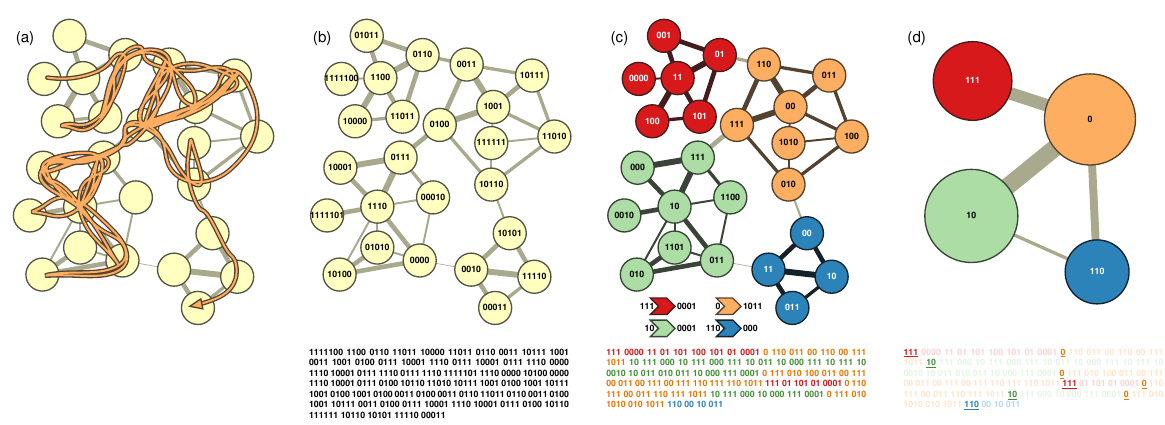
\includegraphics[scale=0.52]{img/1.9_infomap.png}
\par\bigskip
\small Fuente: \citet{2009_Rosvall_MapEquation}
\end{minipage}\bigskip
\begin{description}
    \setlength\itemsep{0em}
    \item[(a)] El objetivo es describir efectiva y concisamente, la trayectoria ---guiada por relaciones ponderadas--- de un caminante aleatorio en una red (línea naranja). 
    \item[(b)] Para una descripción eficiente se utilizan \emph{códigos de Huffman}; donde cada vértice es representado por un código binario único, y la secuencia de códigos ---indicada por la cadena de 314 bits bajo la red--- describe completamente la trayectoria en (a)\footnote{
	Para evitar secuencias ambiguas, ningún código debe ser prefijo de otro, de modo que su concatenación (sin puntuaciones) pueda ser interpretable.}. 
    Vértices visitados con mayor frecuencia tienen un identificador más corto, mientras que vértices que se visitan con menor frecuencia tienen un código de mayor longitud. 
    \item[(c)] Es posible generar una codificación como la anterior, pero en dos niveles diferenciados, lo cual reduce la longitud de la descripción sin pérdidas de información\footnote{
	En este ejemplo, la cadena es reducida a una de 243 bits, y en promedio \citet{2009_Rosvall_MapEquation} refieren que las cadenas son un 32\% más cortas.}. 
    En un nivel superior, se crea un \emph{índice de libro de códigos} ---mostrado bajo la red---, que señala el inicio y fin de un fragmento de la trayectoria dentro de un \emph{módulo}, determinado por la persistencia con la que una caminata aleatoria visita ciertos miembros bien conectados. 
    En un segundo nivel se codifican vértices individuales, que requieren de la especificación de su libro de códigos ---índice de inicio anterior, relacionado al módulo que pertenecen--- para ser identificados de forma única; a su vez, para especificar el final de un fragmento de la trayectoria en un módulo se especifica el índice final único correspondiente. 
    En su conjunto ambos niveles crean la cadena coloreada mostrada en el extremo inferior ---donde cada color es asociado a un módulo---. 
    \item[(d)] Se reportan solamente los índices que marcan el inicio de un fragmento de la trayectoria dentro de un módulo; donde cada módulo puede ser interpretado como una \emph{comunidad}. 
\end{description}


De modo que ``la partición con la longitud de descripción más corta es la que mejor captura la estructura de comunidad en la red con respecto a su dinámica'' \citep[6]{2014_Rosvall_CommunityMapEq}; hallar dicha partición óptima es el propósito de \emph{Infomap}. 

Formalmente, para una red de orden $N$ con relaciones ponderadas $w_{\alpha \beta}$ entre los vértices $\alpha, \beta \text{ } \epsilon \text{ } V(G)$, la probabilidad condicional de que un caminante aleatorio se traslade del vértice $\alpha$ al vértice $\beta$ está dada por el peso relativo de la arista que los une, en relación a todos los pesos incidentes a $\alpha$: 
\begin{equation*}
    p_{\alpha \rightarrow \beta} = \frac{w_{\alpha \beta}}{\sum_{\beta}w_{\alpha \beta}}.
\end{equation*} 
Una caminata aleatoria en un grafo $G$ comienza ($t=0$) en un vértice cualquiera, y se traslada con probabilidad $p_{\alpha \rightarrow \beta}$ a un nuevo vértice en cada paso subsecuente $t=\{1,2,3,...\}$. 
De forma que para cada paso $t$ se determina una distribución por medio de un vector de longitud $N$, que señala la probabilidad del caminante de estar en cada vértice. 
Donde (suponiendo una red simple ponderada) existe una \emph{distribución estacionaria} $p_{\alpha}$, tal que $p_{\alpha}^{T} = p_{\alpha}^{T}P$\footnote{
    $P$ es la matriz de transición, cuyas entradas son iguales a $p_{\alpha \rightarrow \beta}$ si $\alpha$ es adyacente a $\beta$ o cero de otra forma. 
    Para cada paso, la distribución de probabilidad es actualizada en función del paso anterior como: $p_{t+1}^{T}=p_{t}^{T}P$, de modo que una vez que se alcanza la distribución estacionaria $p_{\alpha}$, esta no cambiará en pasos posteriores. 
}. 
Los valores de dicha distribución son interpretados como ``tasas de visita'', con los que se caracteriza cada vértice. 


Según \citet{2009_Rosvall_MapEquation}, al considerar códigos de Huffman en dos niveles ---para una partición $M$ con $m$ módulos, donde cada vértice $\alpha$ es asignado a un módulo $i$--- se utilizan $m$ \emph{libros de códigos}\footnote{
    Como en el ejemplo anterior, la longitud de los códigos individuales son derivados por las frecuencias con las que un caminante aleatorio visita cada uno de los vértices en el módulo ($p_{\alpha\text{ }\epsilon\text{ }i}$), y sale del mismo ($q_{i}\curvearrowright$). 
} y un \emph{índice de libro de códigos}\footnote{
    De forma similar, la longitud de un índice es derivada del conjunto de frecuencias por el cual un caminante aleatorio entra a cada módulo ($q_{i}\curvearrowleft$). 
} para describir la trayectoria de un caminante aleatorio \emph{entre módulos} ---como se ejemplifica en la figura \ref{1.9_infomap} (c)---.
De manera que tanto la longitud de la descripción, como la tasa de uso de cada libro de códigos pueden ser expresadas en términos de las tasas de visita por vértice $p_{\alpha}$ y las proporciones de transición entre módulos $q_{i}\curvearrowleft$ y $q_{i}\curvearrowright$, con las que un caminante aleatorio entra y sale de cada módulo $i$, respectivamente: 
\begin{equation*}
    q_{i}\curvearrowleft = \sum_{\alpha \text{ }\epsilon\text{ } j\neq i, \beta \text{ }\epsilon\text{ } i} q_{\alpha \rightarrow \beta}
\end{equation*} 
\begin{equation*}
    q_{i}\curvearrowright = \sum_{\alpha \text{ }\epsilon\text{ } i, \beta \text{ }\epsilon\text{ } j\neq i} q_{\alpha \rightarrow \beta}. 
\end{equation*} 

Es decir, que para asignar cada vértice a un módulo, \emph{infomap} se centra en \emph{minimizar la longitud en bits} de la descripción ---en dos niveles, para códigos de Huffman--- de una distribución estacionaria, dado un caminante aleatorio en una red ponderada. 
Donde tal longitud $L(M)$ es calculada por medio de \emph{the map equation} ---ecuación \ref{eq:map_eq}---, cuya base es el \emph{teorema de codificación de fuentes} de Shannon, el cual:
\begin{center}
    \begin{minipage}{0.9\linewidth}
        {\setlength{\parindent}{12pt}\small
        ... afirma que el límite inferior por paso para describir un flujo de $n$ variables aleatorias independientes e idénticamente distribuidas es dado por la entropía de su distribución de probabilidad.
        Es decir, dada la distribución de probabilidad $P = \{p_{i}\}$ tal que $\sum_{i}p_{i} = 1$, el límite inferior de la longitud de código por paso viene dado por: 
        \begin{equation}\label{eq:Shannon}
        L(P) = H(P) \equiv -\sum_{i}p_{i}\log p_{i}.
        \end{equation}
        con el logaritmo tomado en base 2 para medir la longitud de código en bits. \normalsize \citep[8]{2014_Rosvall_CommunityMapEq}.
        }
    \end{minipage}
\end{center}


Así, para calcular el límite inferior de la longitud promedio del código que describe un paso del caminante aleatorio bajo una partición $M$, se pondera la longitud promedio de los índices y códigos en cada módulo según sus tasas de uso: 
\begin{equation}\label{eq:map_eq}
    L(M) = q\curvearrowleft H(Q) + \sum_{i=1}^{m}p_{i}\circlearrowright H(P_{i}), 
\end{equation} 
donde: 
\begin{description}
    \setlength\itemsep{0em}
    \item[$\mathbf{ q\curvearrowleft } = \sum_{i=1}^{m}q_{i}\curvearrowleft $.] Es la proporción por paso con la que cada índice de libro de códigos es utilizado, dado por la suma de las frecuencias con las que el caminante aleatorio entra en cualquiera de los $m$ módulos. 
    \item[$\mathbf{ H(Q) } = -\sum_{i=1}^{m}(q_{i}\curvearrowleft/q\curvearrowleft)\log(q_{i}\curvearrowleft/q\curvearrowleft) $.] La longitud promedio ponderada de la frecuencia con la que cada índice de libro de códigos es usado. La entropía de las tasas relativas de uso mide la longitud promedio más pequeña de los índices que es teóricamente posible asignar a cada módulo $i$. 
    \item[$\mathbf{ p_{i}\circlearrowright } = \sum_{\alpha\text{ }\epsilon\text{ }i}p_{\alpha}+q_{i}\curvearrowright $.] La proporción con la que cada libro de códigos del módulo $i$ es utilizado, dado por la probabilidad de visitar cada vértice más la probabilidad de que el caminante aleatorio salga del módulo. 
    \item[$\mathbf{ H(P_{i}) } = -(q_{i}\curvearrowright/p_{i}\circlearrowright)\log(q_{i}\curvearrowright/p_{i}\circlearrowright)-\sum_{\alpha\text{ }\epsilon\text{ }i}(p_{\alpha}/p_{i}\circlearrowright)\log(p_{\alpha}/p_{i}\circlearrowright) $.] La longitud promedio ponderada de la frecuencia con la que cada código por vértice, en el módulo $i$ es usado. La entropía de las tasas relativas por las que el caminante aleatorio sale del módulo $i$ y visita cada vértice en el módulo $i$ mide la longitud del código promedio más pequeño que es teóricamente posible. 
\end{description}


Bajo este enfoque, \citet{2014_Rosvall_CommunityMapEq} refieren posibles generalizaciones a estructuras de mayor orden (jerárquicas, superpuestas o dinámicas de Markov). 
En su forma más básica \emph{Infomap} utiliza dos algoritmos diferentes, para identificar soluciones en dos o más niveles; aquí sólo utilizamos el primer método. 


El núcleo para el algoritmo en dos niveles toma vértices adyacentes, los cuales une en módulos, que posteriormente une en supermódulos y así sucesivamente. 
Primero, cada vértice es asignado a su propio módulo; después, bajo un orden secuencial aleatorio, cada módulo es unido al módulo adyacente que resulta en el mayor decremento de la ecuación \ref{eq:map_eq} ---si no hay ninguna disminución, el módulo no se une a ningún otro---. 
El proceso se repite sucesivamente para módulos de mayor orden (mezclados de forma similar) hasta que la longitud de la descripción no se pueda reducir más. 


Sin embargo, ya que es posible quedar estancado en un mínimo local, se mejora la precisión del algoritmo separando los módulos de la partición final por alguno de los siguientes métodos: 

\begin{itemize}
    \item \emph{Movimientos de submódulos}. Donde cada módulo es tratado como una red, en la cual se aplica el núcleo del algoritmo, generando uno o más submódulos. 
    Luego, al considerar los módulos de la partición original, el algoritmo principal se vuelve a aplicar en los submódulos, permitiendo que cada uno de ellos pueda ser vinculado a un módulo diferente. 
    \item \emph{Movimientos de un sólo vértice}. Como al inicio del algoritmo, cada vértice es asociado a su propio módulo. 
    Y bajo los módulos de la partición original, el algoritmo principal se vuelve a aplicar, de modo que cada vértice pueda ser movido a un módulo diferente. 
\end{itemize}


\begin{center}
    \begin{minipage}{0.9\linewidth}
        {\setlength{\parindent}{12pt}\small
        En la práctica, repetimos las dos extensiones al algoritmo central en secuencia y siempre que se mejore la agrupación. 
        Además, aplicamos los movimientos de submódulos recursivamente. 
        Es decir, para encontrar los submódulos que se moverán, el algoritmo primero divide los submódulos en sub-submódulos, sub-sub-submodulos, y así sucesivamente hasta que no sean posibles más divisiones. 
        Finalmente, dado que el algoritmo es estocástico y rápido, podemos reiniciar el algoritmo desde cero cada vez que la agrupación no puede mejorarse más y el algoritmo se detiene. 
        La implementación es sencilla y, si se repite la búsqueda más de una vez, 100 veces o más si es posible, es menos probable que la partición final corresponda a un mínimo local. 
        Para cada iteración, registramos la agrupación si la longitud de la descripción es más corta que la mínima longitud de la descripción anterior. \normalsize \citep[12]{2014_Rosvall_CommunityMapEq}.
        }
    \end{minipage}
\end{center}






\subsubsection{Comunidades por modelo de bloques: Clustering jerárquico}
\label{sec:ClasesEquivalentes}

El \emph{clustering jerárquico} es un conjunto de técnicas aglomerativas que identifican posiciones distinguibles o \emph{clases de equivalencia} (también referidas como \emph{bloques} o comunidades), basadas ---en nuestro caso--- en los conceptos de equivalencia estructural o regular. 
Es decir, que tales bloques serán conformados por vértices con una alta similaridad, según las medidas presentadas en la sección \ref{sec:EquivalenciaYSimilaridad}\footnote{
    Aunque las implementaciones computacionales más comunes utilizan su complemento (es decir, medidas de disimilitud) o bien, \emph{distancias}. 
    Por otro lado, hay una gran cantidad de similaridades que pueden ser utilizadas también. 
    Donde la elección de una medida particular, según \citet{2010_Newman_Networks}, es determinada más a menudo por la experiencia o experimentación que por una remisión a conceptos fundamentales. 
}. 


Al ser un método fácilmente interpretable cuando se utiliza una medida de similaridad estructural, de acuerdo a \citet{1994_Wasserman_SNA}, este es ampliamente utilizado dentro de las ciencias sociales para determinar subgrupos cohesivos\footnote{
    Empleando distintas medidas de similaridad, y ocasionalmente diferentes algoritmos de optimización, \citep[2]{2006_Newman_Similarity}.
}. 
De modo que será relevante tratar de establecer una partición óptima (si esta existe) que divida claramente a grupos de actores por las relaciones análogas que comparten hacia otros. 


Por otra parte, al utilizar la similaridad de Katz ---basada en equivalencia regular--- en la misma red, sería posible identificar diferentes bloques de vértices, no necesariamente adyacentes, pero cuyos patrones de conexión (dados los vértices a los que se conectan) son parecidos entre sí\footnote{
    Aunque esta es una medida inusual para la agrupación de vértices, \citet{2010_Newman_Networks} sugiere que esta podría ser adecuada para identificar comunidades; por su parte, \citet{2018_Duricic_RegularEquivalence} refieren resultados apropiados para identificar vértices semejantes en redes de confianza. 
}. 
Además, al incorporar similaridades a priori en el último término de las ecuaciones \ref{eq:similaridad_regular} o \ref{eq:similaridad_regular_normalizada}, es posible incorporar el \emph{contexto social} de los actores relacionados, caracterizable por diversos atributos coincidentes entre ellos, asociables al desempeño de roles sociales. 

No obstante, ya que estas similaridades se definen para pares de vértices (no agrupados), se pueden presentar algunos conflictos que dificultan establecer una partición de forma única: 

\begin{center}
    \begin{minipage}{0.9\linewidth}
        {\setlength{\parindent}{12pt}\small
         Supongamos que los vértices $a$ y $b$ tienen una gran similitud, al igual que los vértices $b$ y $c$. 
         Por lo tanto, uno podría argumentar que $a$, $b$ y $c$ deberían estar todos juntos en un grupo. 
         Pero supongamos que $a$ y $c$ tienen una baja similitud. 
         Ahora tenemos un dilema. ¿Deberían $a$ y $c$ estar en el mismo grupo o no?
         \normalsize \citep[381]{2010_Newman_Networks}.
        }
    \end{minipage}
\end{center}


Una generalización sobre el funcionamiento básico del \emph{clustering jerárquico} es presentada por \citet{2010_Newman_Networks} en cinco pasos:
\vspace{-0.5em}
\begin{enumerate}
    \setlength\itemsep{0em}
    \item Elegir una medida de similaridad y calcularla para cada par de vértices. 
    \item Asignar cada vértice a un grupo propio, formado por ese único vértice. 
    \item Hallar un par de grupos con mayor similaridad y unirlos entre sí.
    \item Calcular la similitud entre el nuevo grupo compuesto y todos los demás. 
    \item Repetir los pasos 3 y 4 hasta que todos los vértices hayan sido unidos en uno solo. 
\end{enumerate}

El calculo de similitud entre grupos descrito en el paso 4 es denominado \emph{criterio de enlace}, el cual resuelve el anterior dilema, estableciendo un principio único que evita ambigüedades sobre como debería ser constituida la similaridad del grupo con respecto a otros\footnote{
    Y por extensión, el tipo de unión que se busca entre los miembros de cada grupo. 
}; por supuesto, diferentes criterios resultarán en diferentes estructuras jerárquicas y (potencialmente) nos conducirán a diferentes conclusiones. 
Los resultados de esta aglomeración sucesiva pueden representarse fácilmente a través de un dendrograma, que permite visualizar las relaciones de agrupación entre los vértices, donde el eje vertical muestra las proximidades máximas (o diferencias mínimas) entre grupos. 



Algunos de los criterios de enlace más utilizados implican asignar la mayor similaridad previa\footnote{
    Suponiendo la existencia de tres grupos $c_1$, $c_2$ y $c_3$, donde una medida de similaridad está definida para cada par de grupos $s(c_i,c_j)$, de modo que $c_1$ y $c_2$ son unidos ---al tener la máxima similaridad, según se describe en el paso 3 anterior--- en un nuevo grupo $c_n$; este criterio asignaría $s(c_n,c_3) = max( s(c_1,c_3), s(c_2,c_3) )$. 
} (\emph{single linkage}); la mínima (\emph{complete linkage});  su promedio (\emph{average linkage}); el centroide de las disimilaridades de todos sus miembros; o bien, es calculada con base en principios adicionales\footnote{
    Mientras que algunos de estos criterios sólo precisan de los resultados de una similaridad (o su complemento), otros requieren (por el bien de la corrección geométrica) métricas de distancias, definidas en un espacio euclidiano. 
}. 
Un criterio particular debería ser elegido teniendo en cuenta la naturaleza de la red y el tipo de agrupaciones buscadas, en nuestro caso elegimos el \emph{criterio de Ward}, con el cual se unen aquellos grupos en donde se minimice una función objetivo ---de aumento en la suma de cuadrados--- sobre el complemento de las similaridades involucradas\footnote{
    Se minimiza el cambio de varianza o la suma de errores cuadrados por medio de la función objetivo: 
    $\delta^{2}(c_1,c_2) = \frac{|c_1| |c_2|}{|c_1|+|c_2|}||\overrightarrow{c}_{1}-\overrightarrow{c}_{2}||^{2}$, donde $|c|$ es la cardinalidad del grupo $c$, $\overrightarrow{c}$ su centro y $||.||$ es la norma euclidiana. 
    Hay diferentes implementaciones del método, de entre las cuales elegimos \emph{ward.D2}, en la función \emph{hclust()} de \emph{R}. 
}; ya que nos proponemos hallar núcleos de vértices con posiciones tan regularmente cercanas entre sí como sea posible. 


Sea cual sea el criterio de enlace elegido, el proceso crea hasta $N-1$ particiones iterativamente de entre las cuales es común que se escoja sólo una para representar clases de equivalencia. 
Aunque se puede seleccionar una partición visualmente, al identificar un punto de corte adecuado en el dendrograma resultante, este no se considera un buen método y puede ser engañoso. 
Un método objetivo de selección podría ser fijado de acuerdo a la mayor razón de cambio entre el incremento de bloques unidos y la reducción de similaridades entre ellos; no obstante, no siempre es posible hallar este punto de inflexión de forma evidente\footnote{
    Existen distintas variaciones para tratar de fijar un punto o región de inflexión; uno de los más utilizados es el \emph{elbow method}, fijado por el porcentaje de varianza explicado en relación al número de grupos elegidos. 
    En nuestro caso, el índice de Dunn, presentado en la ecuación \ref{indice_Dunn} también podría ser considerado para determinar el óptimo número de grupos; junto a él, el índice de \emph{Davies–Bouldin} y otros métodos han sido fijados para determinar un número óptimo de grupos cuando este se desconoce a priori; sin embargo, se debe considerar los aspectos (o supuestos) en los que cada uno de ellos se basa si se elige alguno como criterio único de selección. 
    Otros métodos cuantitativos incluyen criterios de información, siluetas, permutaciones aleatorias y validación cruzada; existiendo una amplia literatura sobre el tema. 
}. 
Cualitativamente, de acuerdo a \citet{1994_Wasserman_SNA}, la teoría es la mejor guía para elegir un umbral de similaridad que proporcione particiones útiles e interpretables, de acuerdo a las características de la red. 
En este sentido, cada partición de actores involucra distintos niveles de ajuste respecto a la similaridad en que se basan, y cuya utilidad depende de las condiciones específicas del tipo de red analizada. 



Existen varios \emph{índices de validación} para comprobar cuantitativamente qué tan adecuada es la partición creada, utilizamos uno de los más populares llamado ``índice de Dunn''. 
Tal índice, creado por \citet{1973_Dunn_Clusters}, se basa en la noción de que una partición idónea debe contener grupos compactos (es decir, que sus miembros deben tener una pequeña varianza), los cuales estén suficientemente separados uno del otro (es decir, que las medias de cada par de grupos sean lo suficientemente lejanas en relación a las diferencias al  interior del grupo). 
Así, para una partición definida con $n_c$ grupos, se obtiene la menor distancia interior entre dos grupos en relación al máximo diámetro, dado los miembros en cada grupo\footnote{
    Debido a que se consideran máximos y mínimos, se espera que los grupos estén similarmente constituidos (como aquellos que usualmente son producidos bajo del criterio de Ward); no obstante, si uno sólo de ellos tiene un diámetro mucho mayor (en relación al resto) el índice de Dunn disminuirá injustamente su valor. 
}. 
El valor de este índice se encuentra entre cero e infinito y se considera que entre más grande sea, la partición producida será mejor: 


\begin{equation}\label{indice_Dunn}
    ID = 
     \frac{ \operatornamewithlimits{min}\limits_{1 \leq i \leq n_c} \left\{ \operatornamewithlimits{min}\limits_{1 \leq j \leq n_c, i \neq j}   \{ dist(X_i,X_j) \}  \right\}  }{ \operatornamewithlimits{max}\limits_{1 \leq k \leq n_c}  \{diam(X_k)\} }
\end{equation} 



Por último, una observación a tener en cuenta de los métodos de agrupación basados en clustering jerárquico es que: 
\begin{center}
    \begin{minipage}{0.9\linewidth}
        {\setlength{\parindent}{12pt}\small
         La agrupación jerárquica no siempre funciona tan bien (...). 
         En particular, aunque a menudo es adecuado seleccionando los núcleos de los grupos, donde los vértices son muy similares entre sí, tiende a ser menos útil para asignar vértices periféricos a los grupos apropiados. 
         Dichos vértices pueden no ser muy similares a los demás y tienden a quedar fuera del proceso de aglomeración hasta el final. 
         Un resultado común de la agrupación jerárquica es, por lo tanto, un conjunto de núcleos estrechamente unidos rodeados por una colección aislada de vértices únicos o grupos más pequeños. 
         Tal resultado, sin embargo, puede contener una gran cantidad de información valiosa sobre la estructura de red subyacente. 
         \normalsize \citep[384]{2010_Newman_Networks}.
        }
    \end{minipage}
\end{center}





% BEGIN                                                                                                                                                                  .                                                                                                                                                                  .                                                                                                                                                                        .                                                                                                                                                                 .                        CAPITULO II: GENERACIÓN DE DATOS                                                                                                                .                                                                                                                                                                  .                                                                                                                                                                        .                                                                                                                                                                 .                                                                                                                                                                        .                                                                                                                                                                 
\chapter{Generación de datos}
\label{chap:Protestas_y_AEP}

\epigraph{\itshape If you have no idea what your data means stop analyzing it. You are just guessing animals in clouds.}{---Usuario ``Anony-Mousse'', \textit{Comentario en stats.stackexchange.com}}


\begingroup
\small
    El objetivo de este capítulo es justificar y discutir nuestra evidencia. 
    Desarrollamos esta tarea partiendo de una metodología general de recolección de información documental (sección \ref{sec:AEP}), 
    discutiendo sus limitaciones y cuestionamientos más comunes (sección \ref{sec:limitaciones}), 
    y describiendo su implementación y orientación específica en este trabajo (sección \ref{sec:validezLAOMS}). 
    La reflexión sobre nuestras propias debilidades metodológicas y los sesgos potenciales en nuestra evidencia nos incita a aclarar ambigüedades, así como fomentar más estudios en una misma dirección, que utilicen el método y proporcionen contrastes bajo los cuales se avance en el estudio de los movimientos sociales.
\vspace{2em}
\endgroup



Teniendo en cuenta que ``la calidad de tus inferencias será tan buena como la calidad de tu evidencia'' \citep[89]{2010_Franzosi_QNA} consideramos necesario hacer una revisión sobre la metodología desde la cual se ha recolectado nuestra evidencia, exponer sus limitaciones, así como evaluar y presentar los datos derivados. Esto es crucial para realizar un análisis posterior, pues como señala Charles Tilly:

\begin{center}
    \begin{minipage}{0.9\linewidth}
        {\setlength{\parindent}{12pt}\small
        Toda la investigación social empírica descansa, al menos implícitamente, en no una sino dos teorías, una teoría que explica el fenómeno que se estudia y otra que explica la generación de evidencia relacionada con el fenómeno. Las dos teorías necesarias interactúan, estableciendo importantes restricciones la una a la otra. La segunda teoría responde preguntas sobre cómo el fenómeno deja rastros, cómo los analistas pueden observarlos, y cómo pueden reconstruir atributos, elementos, causas y efectos del fenómeno a partir de esos rastros. \citep[248]{2002_Tilly_EventCatalogsAsTheories}.
        }
    \end{minipage}
\end{center}


La generación de datos es particularmente conflictiva en el estudio de los movimientos sociales al no existir consenso sobre definiciones base como \emph{acción colectiva}, \emph{eventos de protesta} o \emph{movimientos sociales}. De modo que las definiciones (y por tanto, las variables muestreadas) son establecidas en función de los intereses particulares de una investigación y su adscripción a un marco teórico más general. 
En oposición a otros campos de estudio cuyas fronteras han sido bien acotadas, Koopmans \& Ruchtt plantean la complejidad del problema:


\begin{center}
    \begin{minipage}{0.9\linewidth}
        {\setlength{\parindent}{12pt}\small
        la investigación sobre movimientos sociales no ha sido especialmente fuerte en la producción de evidencia empíricamente fundamentada para probar sus teorías, o incluso simplemente para establecer los hechos que requieren explicación. (...)
        
        Las debilidades metodológicas en la investigación de movimientos sociales tienen varias razones. Primero, los movimientos sociales tienden a ser fenómenos ``difusos''. No tienen fronteras claras, mucho menos membresía formal, y pueden expandirse o reducirse considerablemente en períodos relativamente cortos de tiempo. En segundo lugar, la acción de un movimiento social puede ocurrir en muchos lugares, desde bosques hasta calles y tribunales. Es muy difícil hacer un seguimiento de todas estas actividades que, en su mayor parte, no quedan registradas por los propios movimientos. En tercer lugar, y probablemente la más importante, los métodos y las fuentes que se utilizan ampliamente en otras partes de las ciencias sociales son de poca ayuda práctica en este campo. \normalsize \citep[123--124]{1999_Koopmans_AEPWhere}.
        }
    \end{minipage}
\end{center}

Los estudios de movimientos sociales, ``más orientados a los problemas que a los métodos'' \citep[4]{2014_DellaPorta_Metodologicalpluralism} pueden producir errores que son viejos conocidos de la estadística: el error aleatorio y el error sistemático. En el mejor de los casos, cuando los problemas surgen por el error aleatorio, los problemas pueden ser reducidos simplemente aumentando el tamaño de la muestra; el error sistemático es más problemático, ya que descansa sobre el diseño de investigación o en los métodos utilizados para obtener datos representativos de nuestra unidad de análisis\footnote{
    Un caso legendario de este tipo de error ocurrió durante de las elecciones presidenciales en Estados Unidos para el año 1936. Donde la revista \emph{Literary Digest} invirtió muchos recursos en hacer una encuesta que anticipara al posible ganador, obteniendo más de dos millones de respuestas de todo el país y fallando estrepitosamente al no considerar el sesgo de su muestra ---orientada a un segmento de la población con mayores recursos económicos---. Es decir, solo obtuvieron una medida precisa de un estrato sesgado.
}.
En este sentido, consideramos fundamental la sentencia de \citet{2005_Ioannidis_FindingsAreFalse} para casos análogos, donde advierte que \emph{la mayoría de los resultados de investigaciones publicados son falsos} y la probabilidad de que esto suceda aumenta cuanto más pequeños sean los estudios conducidos en un campo; cuanto mayor sea la flexibilidad en diseños, definiciones, resultados y modos analíticos; cuando los resultados alcanzados no son comprobados por equipos de investigación independientes y cuando se persigue ante todo una significancia estadística\footnote{
	Aunque sus afirmaciones y corolarios abarcan más casos ---sobre todo del área médica---, recuperamos aquí solo aquellos que consideramos que pueden tener una mayor repercusión en el estudio de la protesta en México.
}.


Describimos y revelamos algunos de los problemas en los datos empleados en este trabajo a fin de desarrollar un entendimiento analítico sobre los mismos, el cual debe ser tomado en cuenta en cualquier conclusión derivada de su análisis. 
Dada la preocupación que este tema ha suscitado entre investigadores sociales, dirigimos algunas de sus discusiones sobre confiabilidad y validez al contexto en el que se han generado nuestros datos. 
También presentamos evidencia comparativa que justifica algunas de sus previsiones, donde utilizamos principalmente un script que extrae textos de medios periodísticos digitales nacionales para hacer dicho balance. 
El balance entre la teoría y los resultados comprobados dista de ser completo y concluyente, pero sugiere una gran cantidad de sesgos sistemáticos e inerciales; algunos ---inevitables--- promovidos desde la única fuente de referencia a la que se ha podido recurrir (diarios de circulación nacional), otros ocasionados por los intereses de la investigación llevada a cabo en el LAOMS (de quien hemos obtenido la base inicial sobre protestas) y algunos más como consecuencia de la falta de rigor metodológico.


La primer sección de este capítulo describe la metodología del \emph{Análisis de Eventos de Protesta} (AEP) como una técnica general para obtener datos sobre protestas, cuya operacionalización es prácticamente única en cada proyecto. Los datos que se analizan en este trabajo fueron recuperados por este método, de modo que su introducción es relevante por su justificación.

La segunda sección representa una crítica general al método, define los problemas de sesgo en la selección de diarios como única fuente de referencia y la de fuentes específicas para extraer información sobre protestas; se indica además como las limitaciones en el muestreo, la conformación de categorías teóricas, la captura e interpretación de los textos periodísticos para transformarlos en datos categóricos pueden afectar la interpretación de los patrones observados en los datos.

La tercera sección realiza una evaluación particular a la implementación del método por el LAOMS y a los datos derivados. Introduce además los datos recabados sobre actores colectivos, que complementan a la base de protestas.



\section{Metodología: el Análisis de Eventos de Protesta (AEP)}
\label{sec:AEP}

Los datos presentados como evidencia en las ciencias sociales pueden ser en distinta medida, cuantitativos y cualitativos, centrando su atención de forma diferenciada en distintos aspectos de un mismo fenómeno. 
Cada método que genera evidencia parte de un diseño de investigación cuyo propósito es la recolección de información fidedigna. 
En el estudio de los movimientos sociales \citet{2014_DellaPorta_Metodologicalpluralism} observa que métodos como el análisis comparativo, la observación participante, el análisis del discurso, las entrevistas en profundidad, las historias de vida, el de grupo de enfoque y el análisis de eventos de protesta son combinados a menudo para obtener un mejor entendimiento sobre las protestas.


Se sabe que diversas instituciones públicas, privadas, sociales y gubernamentales generan de modo sistemático u ocasional datos acerca de protestas, pero éstos no están a menudo abiertos al público\footnote{Lo cual es particularmente cierto para los datos oficiales en México: a pesar de que se ha asegurado la existencia de datos en los 3 órdenes de gobierno que dan cuenta sobre las protestas ocurridas en el territorio nacional, no hay forma de obtener acceso a ellos para propósitos de investigación, salvo en algunos casos excepcionales y sólo de forma agregada \citep[81]{2005_Strawn_Tesis}.}, son sesgados, incompletos (estructural, temporal o geográficamente hablando) y pueden ser recabados a través de metodologías tan opuestas, que hacen imposible su comparación a través del tiempo. 
Frente a esta falta de información y dado que otros métodos resultan a menudo demasiado costosos para obtener una perspectiva general de gran parte de los movimientos sociales producidos en amplias extensiones territoriales, el AEP ofrece una alternativa viable para ``realizar un análisis de contenido sobre fuentes informativas de muy distinto tipo (noticiosas, portales institucionales, comunicados de actores, entre otros) con el propósito de recabar y evaluar sistemáticamente la cantidad y las características de las protestas'' \citep[1]{2017_Urbina_estudiantes}, en palabras del coordinador del LAOMS:


\begin{center}
    \begin{minipage}{0.9\linewidth}
        {\setlength{\parindent}{12pt}\small
        La perspectiva del análisis de eventos de protesta (AEP) corresponde a desarrollos recientes de la sociología de la acción colectiva que intenta mapear, analizar e interpretar la ocurrencia y propiedades de grandes números de protesta por medio de análisis de contenido y técnicas estadísticas, usando principalmente, notas periodísticas y otros registros. 
        Los datos recabados para ese propósito se pueden relacionar con otras variables sociales, políticas y económicas, por ejemplo, para estudiar las causas y consecuencias de las protestas. 
        El AEP requiere de una sólida base empírica para observar las actividades de protesta en grandes áreas geográficas en periodos de varios años. \normalsize \citep[30--31]{2010_Cadena_LAOMS}.
        }
    \end{minipage}
\end{center}

Entre las propiedades de las protestas que resultan de mayor relevancia para el AEP, \citet{2002_Koopmans_AEP} enfatizan: la frecuencia, el tiempo, la duración, la localización, las demandas, el tamaño, las formas, los demandantes y los demandados, así como las consecuencias inmediatas y las reacciones que se producen. 
En contraste con otros trabajos (los cuales son considerados por Koopmans y Rucht como un agregado de eventos individuales donde se tiende a confiar en impresiones y generalizaciones especulativas), se considera al AEP como una metodología con una base empírica mucho más sólida, donde se puede obtener información válida y confiable. 
Además de su capacidad para ir más allá de algunos casos y ejemplos ilustrativos, se consideran como ventajas adicionales el no ser una técnica intrusiva, su capacidad para tratar información no estructurada como datos y su sensibilidad al contexto \citep[337]{2014_Hutter_AEP}.

\citet{2010_Franzosi_QNA} precisa que el objetivo final del AEP es la transformación ``de palabras a números''; lo cual implica hasta cierto punto un enfoque cuantitativo, permitiendo  su combinación con otras técnicas y ofreciendo la posibilidad de incorporar sus datos a diferentes diseños de investigación \citep[336]{2014_Hutter_AEP}. 

Esta metodología cuenta con importantes antecedentes que usualmente son revisados antes de establecer un diseño de investigación propio, \citet{2014_Hutter_AEP} clasifica cuatro generaciones de investigadores que han utilizado el AEP para obtener datos que sustenten sus investigaciones; desde mediados de los 60's hasta la actualidad se han generado importantes avances en el método, la justificación de las categorías establecidas y los resultados obtenidos. 
No obstante, en la práctica cada investigación que utiliza esta perspectiva puede aplicar de forma distinta y hasta opuesta criterios elementales para medir las protestas, como Mark Beissinger indica:

\begin{center}
    \begin{minipage}{0.9\linewidth}
        {\setlength{\parindent}{12pt}\small
        Si bien han surgido ciertas prácticas comunes para garantizar el rigor metodológico, el método ha sido operacionalizado de manera diferente en prácticamente todos los casos en que ha sido utilizado. 
        La estandarización de categorías, definiciones y enfoques entre los objetos de análisis ha permanecido esquiva, y por buenas razones. 
        La ventaja del método ha sido precisamente su adaptabilidad a una amplia variedad de circunstancias, dependiendo de los propósitos del investigador.... Los investigadores deben, en última instancia, tomar decisiones sobre qué formas de acción merecen analizarse, qué características de esas acciones merecen atención, qué fuentes se deben usar para obtener información sobre estos eventos y cómo se debe organizar el proceso de registrar esta información. 
        En un estudio bien formulado, tanto la teoría como el contexto deben interactuar para informar estas elecciones. \normalsize Citado en \citep[341]{2014_Hutter_AEP}.
        }
    \end{minipage}
\end{center}

Las decisiones tomadas son cruciales y se debe considerar que a pesar de que varias de ellas ``parezcan meramente técnicas, pueden tener un impacto considerable en los recursos necesarios y la calidad de los datos (validez y confiabilidad)'' \citep[234--235]{2002_Koopmans_AEP}.




\subsection{Unidad de análisis}
\label{sec:AEP_unidad_analisis}

\citet{2002_Koopmans_AEP} sugieren que la unidad de análisis debe ser acotada dimensionando la naturaleza de los actores, acciones y demandas, así como el contexto de la acción; proporcionando no sólo breves definiciones, sino explicaciones detalladas de sus componentes e incluyendo una discusión de sus casos límites. 
Sentencian además que conceptos estrechos son fáciles de identificar y proporcionan un menor número de casos, mientras que conceptos amplios permiten abordar una gama más amplia de preguntas, pero pueden requerir un trabajo de codificación sustancialmente mayor. 

Tradicionalmente, \citet{1999_Koopmans_AEPWhere} refieren que la unidad de análisis seleccionada ha sido el ``evento de protesta''\footnote{Definido e interpretado de forma diferente, según los intereses de la investigación.}, el cual es establecido por su énfasis en ``poco convencionales'', ``disruptivas'' o ``no rutinarias'' formas de acción colectiva. 
Ya que esta visión es criticable por ofrecer una perspectiva truncada en los repertorios de acción de grupos no institucionales, así como de la penetración de demandas de cambio social en políticas institucionales, \citet{2002_Koopmans_AEP} refieren unidades opcionales como ``evento de activación política'', ``reunión contenciosa'' o, más inclusivamente, ``reclamo político''. 
Por último, \citet{2014_Hutter_AEP}  señala que investigaciones más recientes, en un intento por capturar aspectos relacionales de contención política, refieren a un conjunto más amplio de actividades o a una desagregación del ``evento'' en \emph{demandas políticas}, \emph{oraciones principales} o \emph{tripletas semánticas} sustraídas de los textos de referencia.


Distintas unidades de análisis pueden ser incorporadas en un mismo estudio, bajo la agregación o desagregación del evento de protesta o sus variantes. 
Como ejemplo, \citet{2003_Wada_Tesis} recupera \emph{acciones} individuales o colectivas a través de tripletas semánticas, basándose en la estructura simple \emph{Subject-Verb-Object} del idioma inglés; agrupa en un segundo nivel múltiples secuencias de acciones, vinculadas por actores, lugares y agendas comunes en \emph{eventos} y finalmente considera como tercer nivel articulado a las \emph{campañas}, las cuales se componen de un agregado de eventos coordinados, más allá del tiempo y del espacio, que son llevados a cabo por uno o más actores que comparten objetivos comunes. 

\citet{2002_Koopmans_AEP} sugieren además el gran potencial\footnote{Y la gran dificultad para obtener esta información, que pueden ser recopilada de fuentes oficiales, de la misma fuente empleada para medir nuestra unidad de análisis o utilizando métodos de investigación independientes ---lo cual puede ser equiparable a realizar una investigación paralela, dado el coste implicado---.} de datos covariables, sobre potenciales causas y consecuencias vinculadas a protestas, que complementen nuestra unidad de análisis principal, ya que de otra forma los usos del AEP se mantendrán en gran parte descriptivos. 
Entre los tipos de datos que pueden ser recabados se mencionan los recursos de organizaciones, oportunidades políticas y estructuras de alianza, conflicto y discursivas.

La selección de la unidad de análisis depende del enfoque de la investigación, pero también de la capacidad para medirla adecuadamente en el tiempo y espacio delimitados, en función de los recursos obtenidos, pues ``la pregunta de investigación más brillante seguirá sin respuesta si te has quedado sin tiempo o dinero en el camino'' \citep[149]{2010_Franzosi_QNA}. 
Otra limitación estriba en las fuentes disponibles consideradas, pues estas pueden no contienen suficiente información para responder los planteamientos iniciales. 

Aunque existen distintas alternativas para seleccionar la unidad de análisis, todas ellas tienen distintas ventajas y limitaciones analíticas que deben ser consideradas. 
En relación al evento de protesta, se ha sugerido que anteriores unidades de análisis\footnote{
Por ejemplo, ``organización de los movimientos sociales'', ``industria de movimientos sociales'' o ``campaña colectiva''.} ``tendían, intencionalmente o no, a impulsar la investigación sobre la protesta hacia una suposición de existencia o pre-existencia de organizaciones y esfuerzos organizados hacia la movilización popular'' \citep[21]{2005_Strawn_Tesis}. 
Debido a que nuestros datos están basados en el evento de protesta, y ya que es un concepto central en este trabajo, presentamos la definición adoptada por \citet{2017_Cadena_ManualLAOMS}:

\begin{definition}[Evento de protesta]
\label{EP}
	Acción colectiva, que presenta demandas a otros, que emplea uno o varios repertorios de protesta, que se desarrolla en un lugar y en un momento determinados y que transcurre en el espacio público\footnote{Para aclarar algunos conceptos ambiguos, se recomienda consultar el \nameref{AnexoI}, donde se presentan definiciones del LAOMS para varios de los términos empleados.}.
\end{definition}



\subsection{Selección de fuentes}
\label{sec:AEP_seleccionFuentes}

Aunque el AEP establece que se pueden utilizar fuentes de diferente tipo para realizar análisis de contenido, lo cierto es que la mayoría de las opciones ofrecen información pobre e inconsistente: los reportes policiales usualmente son incompletos e incomparables entre pequeñas regiones, la información proveniente de grupos que participan en protestas de forma regular proporcionan una sobrerrepresentación de estos grupos y usualmente solo son útiles si se estudia su movimiento particular, los servicios electrónicos de noticias generalmente no ofrecen noticias de periodos distantes y las agencias de noticias (en el caso de México) no son fácilmente accesibles para particulares y pueden implicar un gasto adicional. 
Como consecuencia, la mayor parte de investigaciones que se basan en el AEP utilizan periódicos locales o nacionales. 
Aunque cada investigador que utiliza el AEP, según \citet{2002_Koopmans_AEP}, reconoce que los reportajes periodísticos no proporcionan una muestra representativa de todo el universo de la protesta\footnote{
    De hecho, datos comparativos sugieren que ``ningún medio de comunicación o fuente policial capta todos, o incluso una muestra representativa, de los eventos de interés. Cada fuente tiene una orientación distinta en su cobertura'' \citep[132]{2001_Maney_Oliver__FindingEvents}.
}, 
la mayoría reconoce que estos ofrecen amplias ventajas comparativas; ya que son hasta cierto punto consistentes, sus reportes son diarios, son baratos, de fácil acceso y proporcionan un reporte más detallado que otros medios de comunicación.

Considerando a los diarios como única fuente de referencia, no hay consenso sobre el tipo de diarios que se deberían seleccionar, por lo que esto debe ser decidido para cada investigación. 
Se pueden elegir, por ejemplo, diarios reconocidos por ser objetivos, que cuenten con una mayor reputación y calidad\footnote{Si bien estos son conceptos abstractos y subjetivos, \citet{1996_MorenoDeAlba_Prestigio} identifica algunos elementos distinguibles en este tipo de fuentes por el tipo de contenido que ofrecen, su formato y su percepción entre los lectores de este tipo de publicaciones.}, argumentando que estos tratan de mantener su credibilidad cubriendo eventos de protesta con una mayor precisión; también se puede realizar esta selección por criterios que se suponen objetivos como ``el diario que genere una mayor cantidad de reportajes sobre protestas'', ``el que se haya mantenido durante más tiempo en circulación'', ``el que tenga más tiraje'' o ``aquel con una red más amplia de corresponsales en las regiones de interés''; otra alternativa, propuesta por autores como \citet{2003_Wada_Tesis} propone seleccionar nuestras fuentes por representar diferentes, importantes e influyentes segmentos de la esfera pública (por ejemplo, medios importantes reconocidos por su tendencia de derecha o de izquierda).

Aún ante la posibilidad de usar varios medios periodísticos de referencia, se pueden identificar dos perspectivas encontradas.
Investigadores como \citet{2002_Koopmans_AEP} sugieren utilizar tantas fuentes como sea posible con el objetivo de recolectar una mayor cantidad de información sobre los eventos de interés (mezclando la información de los eventos reportados más de una vez); mientras que otros como \citet{2003_Wada_Tesis} y \citet{2010_Franzosi_QNA} sugieren la selección de unos pocos diarios para estudiar mejor su sesgo y aumentar la confiabilidad de los datos (manteniendo los datos producidos por cada fuente de forma separada, creando múltiples bases de datos que reflejen la perspectiva individual de cada medio sobre los eventos que reportan).


La figura \ref{2.1_sesgoSeleccion} puede ayudarnos a entender la limitada muestra que generan los diarios; en ella se muestran 3 conjuntos diferentes: $A$ puede representar el universo de todos los eventos de protesta que ocurren para un tiempo y espacio determinados, $B$ es subconjunto de $A$ y en él se consideran los eventos de protesta que son reportados por los medios periodísticos, finalmente $C$ es subconjunto de $B$ y contiene una muestra extraída de notas periodísticas que reportan eventos de protesta. 
Resulta demasiado arriesgado asegurar que $C$ es una muestra representativa de $A$, sobre todo considerando la limitante que ``reside en la ausencia de un parangón objetivo de comparación, el cual a falta de un marco muestral exacto que detalle el total de eventos de protesta (EP’s) que tienen lugar a lo largo de un día, un mes o un año, impide estimar un margen de error aproximado en los datos acumulados'' \citep[2]{2017_Urbina_estudiantes}. 

\begin{minipage}{\linewidth}
\centering
\captionof{figure}{Dos niveles de sesgo por selección} \label{2.1_sesgoSeleccion}
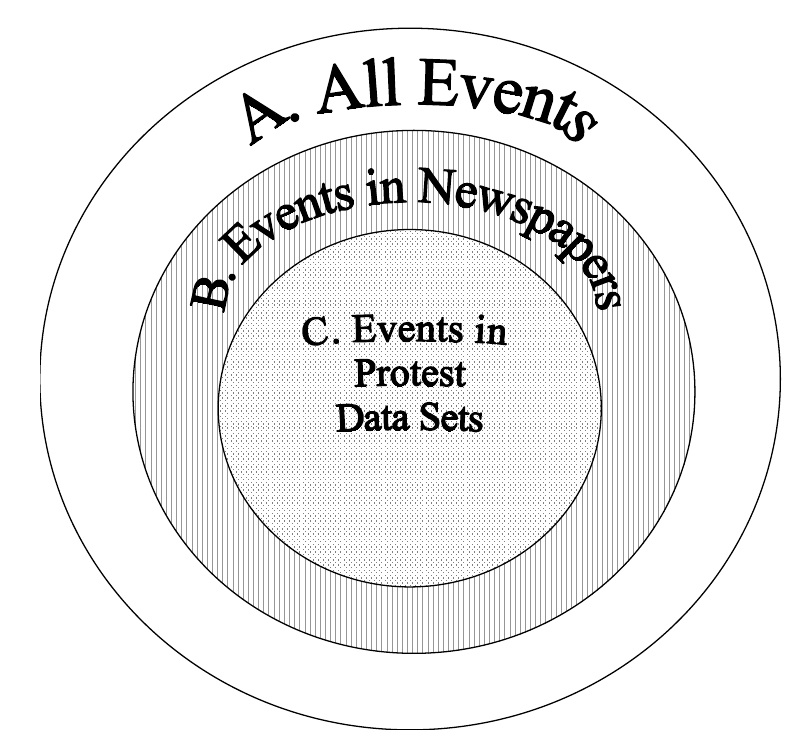
\includegraphics[scale=0.16]{img/2.1_sesgoSeleccion.png}
\par\bigskip
\small Fuente: \citep[6]{2005_Ortiz_NewspaperData}
\end{minipage}\bigskip

Aunque no estemos en posibilidad de saber con precisión el tipo de representatividad que brinda el medio, se sugiere conocer bien las fuentes seleccionadas y los posibles conflictos entorno al sesgo por sus consecuencias en el análisis, como lo indican Koopmans \& Rucht:

\begin{center}
    \begin{minipage}{0.9\linewidth}
        {\setlength{\parindent}{12pt}\small
        Si seguimos ciegamente los informes de los medios, podríamos estar totalmente equivocados al hacer inferencias sobre el universo de todas las protestas en un lugar y tiempo determinados. 
        Los medios no reflejan este universo de ninguna manera representativa. Seleccionan de acuerdo a sus propios criterios y siguen ciclos de atención sobre temas que, sin embargo, pueden ser investigados empíricamente. 
        La evaluación, o  incluso la comprobación cuantitativa, de la selectividad de las fuentes de las que se extrae la información es crucial para todo tipo de AEP. \normalsize \citep[246]{2002_Koopmans_AEP}.
        }
    \end{minipage}
\end{center}


Al respecto, existe un fuerte debate ---ver sección \ref{sec:limitaciones}--- con visiones encontradas sobre la gravedad del sesgo y la posibilidad de anticiparlo. 
Ya que no existen pautas generales para evaluar la representatividad de nuestras fuentes, esto dependerá en última instancia del nivel geográfico, periodo de tiempo, contexto político y área temática cubierta por un estudio \citep[439]{2014_Hutter_AEP}. 
Con el propósito de acotar la discusión y debido a la conformación de nuestra propia base de datos, en adelante consideraremos únicamente medios periodísticos como fuentes utilizables en el AEP.



\subsection{Interpretación a los datos sustraídos de fuentes periodísticas}
\label{sec:Interpretacion_fuentes}

Un aspecto central del debate que surge al seleccionar a los medios periodísticos como principal (o única) fuente, es la interpretación que se debe dar a los datos que han sido recolectados. 
Si los reportajes periodísticos no ofrecen una muestra representativa de todo el universo de la protesta, entonces ¿cuál es su significado? Ya que no existe acuerdo, presentamos las perspectivas predominantes, identificadas por \citet{2003_Wada_Tesis}.



\subsubsection{Perspectiva de estimación del universo}
\label{sec:estimacion_universo}

La mayor parte de los investigadores recurren a esta perspectiva desde diversos enfoques particulares. 
Aunque en ella se reconoce en distinta medida que los diarios no reflejan adecuadamente el universo de la protesta por sus sesgos, su objetivo es la aproximación a dicho universo. 
Sin embargo, esta presunción supone la estabilidad del sesgo en el tiempo, el cual puede ser debatible basándonos en datos empíricos ---ver secciones \ref{sec:Sesgo_circuito_mediatico} y \ref{sec:Sesgo_periodico}---.


\begin{description}
    \item[i] \emph{Enfoque de fuentes complementarias:}  La idea es utilizar a distintos medios para obtener una imagen más completa del universo de la protesta, suponiendo que entre más diarios se utilicen, más cerca nos encontraremos del universo real. 
    Aunque es verdad que de esta forma es posible recolectar un mayor número de eventos, no existe garantía de que nuestra muestra final sea representativa del universo total, existiendo el riesgo de agregar sesgos adicionales no dimensionados cuando se mezclan las fuentes\footnote{Motivo por el cual, se ha argumentado que la utilización de pocas fuentes es mejor, debido a que los sesgos se pueden tratar (o por lo menos entender) más fácilmente si ocurren sistemáticamente.}.
    
    \item[ii] \emph{Enfoque de identificación de sesgo:}  Este enfoque surge ante la preocupación de analizar simplemente patrones noticiosos de los medios periodísticos y no lo que sucede realmente con las protestas; su propuesta consiste en construir ``teoría de medios'' que nos permita conocer los criterios bajo los cuales se seleccionan protestas específicas para cubrir, reportar, editar y publicar. 
    Su limitación reside en que el enfoque sólo nos sugiere la naturaleza de sesgos potenciales sin mostrarnos cómo corregirlos. 
    Si suponemos además que el sesgo no necesariamente permanece estable, existe la posibilidad de invalidar extenuantes análisis de las fuentes en un periodo relativamente corto de tiempo.
    
    \item[iii] \emph{Enfoque del umbral más alto:}  Se trata de obtener estimaciones más precisas de cierta parte del universo de la protesta, filtrando aquellos reportes sobre eventos que son considerados ``sumamente válidos'', en relación a las características que (de acuerdo al enfoque anterior) hacen a un evento más susceptible de ser reportado por los medios periodísticos; limitando, por ejemplo, su tamaño, violencia o duración. 
    Aunque esto puede brindarnos una mejor aproximación respecto a eventos con estas características, el método pierde generalidad sobre el estudio de la protesta.
    
    \item[iv] \emph{Enfoque de corrección de sesgo:}  También supone la identificación del sesgo, proponiendo que una vez conocido, es posible obtener un número aproximado de protestas reales a través de la extrapolación de nuestros datos; se usan modelos de regresión, donde la cobertura periodística es considerada una variable dependiente y las características que hacen a un evento de protesta más susceptible de ser reportado son variables independientes a las que se debe asociar un coeficiente de regresión. 
    El principal problema de este enfoque (además de la suposición de la estabilidad del sesgo), es que usualmente no se cuenta con información necesaria para determinar adecuados coeficientes de regresión para cada contexto periodístico particular.
    
    \item[v] \emph{Enfoque que no ve al sesgo como un problema real:}  Por último, se puede argumentar que el sesgo no representa un problema si nuestro propósito no es reconstruir la verdad absoluta sobre las protestas, sino detectar tendencias en procesos históricos de más amplio alcance, lo cual puede ser efectivo siempre que se pruebe que el sesgo es ``consistente en todas las unidades de análisis'' \citep[253]{2002_Koopmans_AEP}, las preguntas de investigación tengan dicha orientación y el nivel de agregación de variables clave sea lo suficientemente grande como para asegurar la identificación de tendencias \emph{históricas} \citep[352]{2014_Hutter_AEP}.
\end{description}


\subsubsection{Perspectiva de la esfera pública}
\label{sec:esfera_publica}

Como contraposición a la perspectiva que sugiere que es posible, hasta cierto punto, reconstruir el universo de la protesta a partir de los datos muestreados en los diarios, la perspectiva de la esfera pública rechaza la suposición epistemológica de que existe un universo de eventos de eventos de protesta ``diádicos'' donde los manifestantes interactúan con las élites \emph{al margen de los medios}\footnote{
Si bien, la cantidad de protestas que no son visibilizadas en los medios pueden aún ser mayores de las que sí lo son, esta perspectiva los considera como una especie ``diferente'' de eventos, que no han tenido éxito en llamar la atención de los medios periodísticos.}. 
Rechaza además la suposición metodológica de que los medios constituyen un \emph{registro pasivo} de dichos eventos. Como indican Gamson \& Wolfsfeld:


\begin{center}
    \begin{minipage}{0.9\linewidth}
        {\setlength{\parindent}{12pt}\small
        Los movimientos necesitan a los medios de comunicación por tres razones principales: movilización, validación y ampliación de alcance (...), la mayoría de los movimientos deben llegar a su circunscripción en parte a través de una forma de discurso público. 
        El discurso público es transmitido en varios foros, incluyendo las publicaciones del propio movimiento y sus reuniones. 
        Pero el discurso mediático permanece indispensable para la mayoría de los movimientos debido a que la mayoría de las personas que desean alcanzar forman parte de la galería de los medios de comunicación.
        
        (...)
        
        El hecho de que los movimientos necesitan a los medios mucho más de lo que los 	medios los necesitan se traduce en mayor poder para los medios en la transacción. \normalsize \citep[116]{1993_Gamson_medios}.
        }
    \end{minipage}
\end{center}

Más allá de esta relación dual, se sostiene que las protestas muestreadas involucran relaciones triádicas entre manifestantes, élites y medios de comunicación; lo cual nos lleva a redefinir el universo muestreado:


\begin{center}
    \begin{minipage}{0.9\linewidth}
        {\setlength{\parindent}{12pt}\small
        No vemos a los eventos de protesta reportados como una muestra del universo de eventos de protesta diádicos\footnote{Considerando la relación entre manifestantes y élites.} registrados por los medios de comunicación, sino como el universo de eventos de protesta que entran a la esfera pública a través de los medios de comunicación. 
        Mientras que la perspectiva de estimación del universo refiere a los eventos de protesta ``diádicos'' como el único objeto teórico relevante de investigación, la perspectiva de la esfera pública encuentra un valor genuino en estudiar eventos reportados como un objeto legítimo. \normalsize \citep[108]{2003_Wada_Tesis}.
        }
    \end{minipage}
\end{center}


Aunque los datos en este trabajo son entendidos en función de la perspectiva de la esfera pública y pese a que nuestro medio de referencia se considera relevante por su representación como un segmento diferenciado, importante e influyente de dicha esfera como afirma Wada, \citet{2005_Ortiz_NewspaperData} nos recuerdan que (a pesar de que estas preocupaciones se vean reducidas) los problemas de sesgo siguen siendo relevantes y deben ser considerados a fin de evitar posibles malinterpretaciones de análisis.



\subsection{Muestreo para obtener textos}
\label{sec:AEP_MuestreoTextos}

Resulta difícil asegurar la recopilación de todos los eventos de protesta ---así sean solo de un periodo dado--- de una fuente por medio de una lectura rápida del medio y \citet{2014_Hutter_AEP} considera que el proceso de recolección de textos específicos de nuestro interés puede llegar a ser aún más absorbente que el proceso de captura de la información\footnote{Existen reportajes, por ejemplo, que refieren protestas como un tema secundario, por lo que es difícil identificar estos eventos sin leer de forma cuidadosa cada elemento del texto. 
Realizar este tipo de revisión diariamente para todas las secciones del diario que se consideran relevantes, puede asegurar ---siempre bajo un margen de error--- la identificación de las protestas reportadas por un medio, pero el tiempo dedicado a esta actividad puede resultar demasiado elevado.}; según nuestra perspectiva, dejar sin especificar un protocolo riguroso para la recolección de documentos es poco transparente, ya que permite la discrecionalidad de quien realiza la tarea para seleccionar o no una noticia y puede ser causa de errores sistemáticos no reconocidos, sobre todo cuando se extraen grandes cantidades de documentos. 

\citet{2003_Wada_Tesis} indica dos tipos de muestreo posibles: (i) basado en el \emph{tiempo} ---utilizado sobre todo para investigaciones históricas---, haciendo una revisión exhaustiva del diario en un periodo intercalado de días, semanas, meses o años y (ii) basado en \emph{palabras clave} ---considerado el más eficiente y riguroso, recomendado si los textos mantienen un formato digital---, que supone la búsqueda textual de términos significativos (como ``protesta'', ``marcha'' o ``mitin'') de acuerdo a las formas, generalmente verbales, que son consideradas descriptivas de un tipo de evento.

\citet{2001_Maney_Oliver__FindingEvents} identifican como técnica de búsqueda adicional un protocolo \emph{específico de eventos}; basado también en palabras clave, pero donde sus términos son elegidos de forma iterativa\footnote{
Creando términos, encontrando noticias relevantes a partir de ellos y extrayendo de estas noticias nuevos términos, hasta que no se encuentren más términos relevantes.}, 
por su asociación a características de eventos particulares que son de interés para la investigación\footnote{
Por ejemplo, aquellas relacionados con actores, objetivos, fechas, lugares, demandas, acciones y otros elementos discursivos.}. 

Además refieren que es usual que se reduzca el tiempo y atención dedicada a cualquier búsqueda por medio de la lectura focalizada a secciones específicas de un diario; como sus titulares, pies de fotos u otros elementos del mismo.

La pérdida de noticias relevantes es inevitable para cualquier técnica de búsqueda; sin embargo, es posible aproximar el nivel de pérdida y su importancia al evaluar el protocolo utilizado:

\begin{center}
    \begin{minipage}{0.9\linewidth}
        {\setlength{\parindent}{12pt}\small
        Las técnicas de búsqueda tienen importantes implicaciones para la validez del análisis de la cobertura de eventos colectivos públicos reportados en medios. 
        Las técnicas de búsqueda varían en el volumen total, el rango cronológico y los tipos de artículos recuperados de eventos, así como en su sensibilidad a la cobertura de diferentes tipos de eventos. \citep[136]{2001_Maney_Oliver__FindingEvents}.
        }
    \end{minipage}
\end{center}




\subsection{Análisis de contenido y esquemas de codificación}
\label{sec:AEP_analisisContenido}

El AEP puede ser referido como ``un tipo de \emph{análisis de contenido}'' \citep[335]{2014_Hutter_AEP}. 
Aunque \citet{1990_Krippendorff_ContentAnalysis} define al análisis de contenido de forma más general como una técnica de investigación destinada a formular inferencias\footnote{Argumentando que incluso elucidaciones ``puramente descriptivas'' suponen inferencias, por primitivas que sean.} reproducibles y válidas que puedan aplicarse a su contexto (construido por el analista); en el AEP, el análisis de contenido ha sido reconocido por autores como Shapiro y Markoff como ``una técnica de \emph{medición} antes que una técnica de \emph{inferencia}'' ---citado en \citep[122]{2003_Wada_Tesis}---. 
En ese sentido, aunque todo texto incluye significados simbólicos que hacen inevitable cierta inferencia, el AEP propone centrar su atención en la descripción de hechos bajo los cuales se puede caracterizar a la unidad de análisis seleccionada, y (a partir de tales hechos) construir categorías que forman en su conjunto \emph{esquemas de codificación}, con los cuales se pretenden contabilizar tendencias importantes para la investigación de la protesta. 
La conformación de estos esquemas es descrita por Franzosi en los siguientes términos:

\begin{center}
    \begin{minipage}{0.9\linewidth}
        {\setlength{\parindent}{12pt}\small
        Los esquemas de codificación deben derivarse de una teoría política sistemática. Deberían permitir a los investigadores probar hipótesis específicas sobre esa teoría. (...) En realidad, los esquemas del análisis de contenido se han derivado típicamente (inductivamente) de un proceso interactivo entre los intereses iniciales de un investigador, la lectura cuidadosa de textos específicos que abordan dichos intereses de investigación, el diseño de categorías de codificación preliminares (donde esquemas de codificación disponibles de investigaciones pasadas juegan un papel fundamental), la codificación de textos en estas categorías y la refinación de las categorías hasta que el investigador considere que los esquemas de codificación capturan adecuadamente lo dicho en los textos seleccionados a la luz de las necesidades de investigación específicas del investigador. Irónicamente, los investigadores cualitativos recomiendan el mismo enfoque sin contar al final. \normalsize \citep[34]{2010_Franzosi_QNA}.
        }
    \end{minipage}
\end{center}

Es decir, la transformación ``de palabras a números'' implica un enfoque cuantitativo sólo superficialmente y depende en gran medida del marco teórico de referencia. Si bien es cierto que los esquemas de codificación permiten realizar un análisis cuantificable de la información clasificada en función del significado asociado a cada variable (usualmente nominal), existen varias limitantes que restringen el uso de los datos para técnicas estadísticas inferenciales complejas. Para precisar el alcance de los datos (recabados por el AEP y/o de datos de covariables) en un análisis formal, habrá que detallar el tipo de categorías empleadas, evaluando su selectividad, confiabilidad, verificabilidad, comparabilidad, limitación e inclusividad\footnote{
    Pues como afirma \citet{2002_Tilly_EventCatalogsAsTheories}, cualquiera que construya catálogos de eventos se preocupara inevitablemente sobre estos problemas ---o sus críticos lo harán---.
}.

Ya que el AEP implica una técnica que debe ser reconstruida para cada proyecto particular, su validez y confiabilidad como método de investigación depende en gran medida de la implementación (y difusión) de estándares necesarios para su evaluación y replicación \citep[1]{2015_Lacy_BestContentAnalysis}.



\subsection{Captura de información}
\label{sec:AEP_captura}

El proceso de captura en el AEP debería ser (idealmente) un proceso simple, donde de forma natural se ajuste información textual a los esquemas de codificación creados. 
Entendido como un proceso sistemático, \citet{2002_Koopmans_AEP} describen que en primer término se debe leer de forma cuidadosa cada texto recuperado en conjunto con  otros, que puedan ser agregados según la definición de nuestra unidad de análisis; en una segunda etapa, una vez que han sido identificados y delimitados los eventos, estos son capturados de acuerdo al esquema de codificación, archivando por último los textos de referencia. 
Aunque esta es una aproximación popular, el proceso puede ser optimizado según los propósitos de la investigación, la unidad de análisis y la estructura de los textos consultados, de modo que ``solo una comprensión clara de la naturaleza de tus documentos te permitirá tomar la decisión correcta sobre cómo organizar la tarea de codificación'' \normalsize \citep[99]{2010_Franzosi_QNA}. 
Ya que esta tarea resulta demasiado absorbente para que la pueda realizar una sola persona, a menudo se requiere de un equipo dedicado exclusivamente a ello\footnote{Aunque investigaciones recientes han utilizado herramientas programáticas que aprovechan los avances en el procesamiento del lenguaje natural para automatizar de forma parcial o completa este proceso de captura ---ver \citet{2013_Schrodt_automatedPolitical} y \citet{2015_Danilova_Linguistic}---, en el español han existido pocos avances en esta dirección, por lo que en este trabajo no se considera la codificación automática, si bien en algún momento se contempló su implementación en el LAOMS.}.

Resulta de vital importancia asegurar la validez y confiabilidad de los datos capturados, sobre todo si el equipo de captura es grande e inestable. 
Si suponemos como \citet{1990_Krippendorff_ContentAnalysis} que el análisis de contenido supone la realización de inferencias, aún para investigaciones que pretenden capturar datos factuales sobre eventos de protesta, debemos hacer intentos por reducir la discrecionalidad de los capturistas en la interpretación de los textos. 
Un método para conseguir esto es la construcción y actualización constante de manuales de captura que hagan explícita la relación entre información textual y los esquemas de codificación; también se pueden realizar sesiones grupales que produzcan acuerdos sobre el tipo de interpretación dada a ciertos elementos conflictivos de un texto; se pueden realizar además capacitaciones, controles de calidad y seguimiento puntual sobre las dudas de los capturistas; otra posibilidad, es desarrollar plataformas informáticas que agilicen el proceso de codificación y reduzcan fallos no intencionales. 
De forma adicional, \citet{2015_Lacy_BestContentAnalysis} sugieren realizar pruebas sobre la comparabilidad del trabajo de un capturista en distintos periodos de tiempo y con respecto a otros capturistas del equipo a fin de probar la confiabilidad del esquema de codificación y su capacidad para dar como resultado una auténtica categorización de contenido; el objetivo final (sugieren) es asegurar la reproducibilidad de la investigación, manteniendo un alto contenido relevante, independientemente de los grupos particulares de codificadores y sus idiosincrasias.




\section{Limitaciones del AEP}
\label{sec:limitaciones}

Como indican \citet{2002_Koopmans_AEP}, a pesar de las grandes ventajas que podría implicar el AEP, este aún no forma parte del repertorio metodológico estándar en las ciencias sociales; enfrentando como principal objeción la suposición de que ``no representa la realidad''. 
Existen, por supuesto, diferentes puntos de vista de este supuesto\footnote{Y objeciones a cada uno de ellos ---generando una discusión retroalimentada---. 
Por ejemplo, Koopmans \& Rucht, quienes basándose en evidencia empírica aseguran que el supuesto está ---según su perspectiva--- ``basado en una percepción errónea'' \citep[252]{2002_Koopmans_AEP}. 
Pensamos que esto es una posibilidad; pero ya que el método se establece de forma única para cada investigación, se debe comprobar de forma individual la certeza o alcance de esta suposición.}, de los cuales recuperamos aquí los que consideramos más relevantes en función de la perspectiva bajo la cual ha sido planeado y llevado a cabo el proceso de recolección de datos por el LAOMS. 
Valoramos que las críticas expuestas son lo suficientemente fundamentadas y respaldadas para proporcionarnos elementos que nos permitan hacer una evaluación propia sobre los datos que son presentados como evidencia en este trabajo ---ver sección \ref{sec:validezLAOMS}---.

De forma general, clasificamos los conflictos con el método en dos grupos:

\begin{enumerate}
    \item En el primero, compilamos sesgos posibles en función de las etapas necesarias para la selección de una noticia, identificada como relevante al contener referencias mínimas de un evento de protesta ---según la definición \ref{EP}---:
	\begin{enumerate}
	    \item Sesgo asociado a la conformación del circuito mediático (\ref{sec:Sesgo_circuito_mediatico}). 
	    \item Sesgo asociado a la selección de los diarios (\ref{sec:Sesgo_periodico}). Es decir, una vez elegido cierto subconjunto de fuentes, se introducen sesgos por: (i) la línea editorial de las fuentes consideradas, (ii) la práctica y la pericia del reportero, 
	    y (iii) la plataforma de difusión (versiones impresa o en línea de los diarios).
	    \item Sesgo asociado a los protocolos de búsqueda de noticias (\ref{sec:Sesgo_protocolo_busqueda}).
	\end{enumerate}
    \item En el segundo grupo podemos hallar deficiencias en el proceso de transformación de información textual a categórica, que pueden ser generadas por:
	\begin{enumerate}
	    \item Equivocaciones no intencionales en la captura de información (\ref{sec:Sesgo_captura}).
	    \item Interpretación subjetiva de los textos por idiosincrasias personales, conflictivas entre capturistas (\ref{sec:Sesgo_procesamiento}).
	    \item Definición y ajustes de esquemas de codificación, que complejizan la comparabilidad entre datos (\ref{sec:esquemas_de_codificacion}).
	\end{enumerate}

\end{enumerate}




\subsection{Sesgo asociado a la conformación del circuito mediático}
\label{sec:Sesgo_circuito_mediatico}


Aunque con cierta tradición, el AEP es una perspectiva relativamente nueva; \citet{2014_Hutter_AEP} refiere que es en los 90's (bajo el establecimiento de una ``tercera generación'' de investigadores que usan el método) cuando surge una discusión ---mantenida hasta hoy--- sobre los problemas que implica la utilización de diarios como principal fuente de referencia\footnote{Por ejemplo, \citet{1999_BarrancoET_ValidityNewspapers} quienes afirman que el uso de periódicos en estudios de movimientos sociales ha sido basado principalmente en postulados teóricos, en lugar de investigaciones empíricas.}. Aunque ``ninguna fuente de datos está exenta de errores, incluyendo a las estadísticas recopiladas oficialmente'' \citep[7]{1987_Franzosi_Press}, distintos investigadores consideran que:


\begin{center}
    \begin{minipage}{0.9\linewidth}
        {\setlength{\parindent}{12pt}\small
        Es erróneo asumir, sin embargo, que los datos de periódicos son tan buenos como otros datos en ciencias sociales. 
        Los sesgos en otros tipos de datos de ciencias sociales han sido estudiados más exhaustivamente y, debido a que los sesgos son mucho mejor comprendidos, correcciones (al menos parciales) son usadas comúnmente en el análisis. \normalsize \citep[411--412]{2005_Ortiz_NewspaperData}.
        }
    \end{minipage}
\end{center}


Según \citet{2010_Franzosi_QNA}, la obsesión de investigadores que utilizan el análisis de contenido se ha centrado en mejorar la \emph{confiabilidad} de los hallazgos, al asegurar la reproducibilidad de sus mediciones\footnote{
Uno de los principios básicos de la ciencia.} a partir de un mismo grupo de textos e instrumentos de medición, aún cuando se empleen diferentes capturistas. 
Sin embargo, se ha prestado poca atención a la \emph{validez} de tales datos, la cual descansa sobre factores exógenos, derivados de las fuentes que son tomadas como referencia. 
Si bien se han considerado distintas interpretaciones a los datos resultantes ---ver sección \ref{sec:Interpretacion_fuentes}---, debemos identificar puntualmente los factores que pueden desviar en mayor medida nuestro conocimiento sobre los datos producidos.

\begin{center}
    \begin{minipage}{0.9\linewidth}
        {\setlength{\parindent}{12pt}\small
        ¿Cuál es el punto de asegurar el registro de una cifra de 200,000 para el tamaño de una multitud, cuando tal cifra puede en realidad rayar en lo fantástico y cuando, además, existe la misma probabilidad de que se sobreestime o subestime? 
        Dado que es mucho más probable que el error no aleatorio (validez) distorsione los datos históricos que el error aleatorio (confiabilidad) y dada la desproporcionada atención prestada a los problemas de confiabilidad más que de validez, recomendaría un cambio de enfoque, de problemas de confiabilidad a problemas de validez. \citep[151]{2010_Franzosi_QNA}.
        }
    \end{minipage}
\end{center}

Bajo esta visión, aún cifras y hechos que son presentados ``objetivamente'', pueden estar sesgados por los medios periodísticos; más aún, ya que la selectividad de lo que \emph{merece ser reportado} es decidido a discrecionalidad por cada medio, la información que no es descrita sobre un evento puede ser tan significativa como la que se presenta, pues ``el tipo de sesgo más probable en medios de comunicación, sucede más por el silencio y el énfasis que por información falseada abiertamente''\footnote{
    Por lo que podemos pensar que el mayor riesgo es obtener información insuficiente, en lugar de información errónea. Sin embargo, como efecto de una selectividad sistemática, es posible falsear completamente causas, desarrollos y contextos del evento, llegando incluso a incitar a la criminalización de la protesta como sugiere \citet{2013_Rovira_ActivismoMediatico}. 
    Si todos los diarios reportaran los mismos eventos, en teoría podríamos tener una visión más certera al contrastar hechos reportados en distintas fuentes, pero debido a que esto no es así, la comparación puede resultar en la confrontación de sesgos difícilmente evaluables y virtualmente imposibles de anticipar.
} \citep[7]{1987_Franzosi_Press}.
Una acción común en algunos estudios ha sido ignorar la información faltante, siempre que se presente cierta información mínima; suponiendo por ejemplo, ``que si el artículo no menciona detenciones o barricadas policiales, entonces no se realizaron arrestos ni se utilizaron barricadas'' \citep[403--404]{2005_Ortiz_NewspaperData}. 
Otras perspectivas\footnote{
    Aquellas que no ven al sesgo como un problema real.
} consideran que si un diario no ha reportado ciertas características de un evento, es porque estas no eran lo suficientemente relevantes, por lo que pueden ser descartadas sin que se afecte a rasgos generales la ``tendencia'' de la investigación y otros más como \citet{2002_Koopmans_AEP} sugieren que se puede utilizar la mediana de cierto rango de datos para subsanar la información faltante, aún cuando desconocemos a priori el efecto que esta homogeneización pueda tener en nuestras conclusiones finales.


Teniendo en cuenta que ``la cualidad escénica de la protesta social la hace vulnerable a la omisión o a la tergiversación mediática'' \citep[35]{2013_Rovira_ActivismoMediatico} debemos ser cuidadosos al realizar deducciones superficialmente fundamentadas.  
\citet{1987_Franzosi_Press} reúne algunas críticas para señalar que los periódicos difieren ampliamente en sus prácticas informativas y cobertura de noticias; lo que ha llevado a algunos investigadores a asegurar que las noticias son tendenciosas y selectivas, tergiversando particularmente los problemas laborales y de clase, reflejando de forma usual las intenciones, voluntad e intereses de grupos económicos dominantes. 
Existen, también diarios alternativos o aquellos que pretenden ser imparciales; sin embargo, ningún medio es neutro: ``seleccionan, editan, alteran y hasta llegan a manufacturar realidades. Su naturaleza policromática les lleva a desempeñar papeles que van desde el perro guardián, hasta el del perro guía pasando por el del perro faldero'' \citep[7]{2008_ASF_Medios}.


\citet{1992_Gamson_mediosRealidad} enfatizan la producción de \emph{imágenes} antes que \emph{hechos} o \emph{información}, porque esta forma más sutil de significado está en el corazón del problema que determina construcciones sociales de realidad ---realidad simbólica, según \citet{2008_ASF_Medios}---. 
Según sus argumentaciones, recibimos noticias en  ``cápsulas dramáticas incompletas, que hacen difícil ver las conexiones entre asuntos o incluso seguir el desarrollo de un asunto en particular a lo largo del tiempo''\footnote{
Un aspecto trascendente de esta perspectiva es la representación del discurso, ya que las demandas de un movimiento amplio pueden ser introducidas por miembros sin experiencia para hablar y que resultan fácilmente manipulables: ``Les gana la risa. Los simpáticos para la prensa pierden el piso de lo social. No es por azar que se escogen a los voceros. Suelen ser mediáticamente repulsivos'' --- Pablo Romo, de la organización Serapaz \citep[52]{2013_Rovira_ActivismoMediatico}---.} ---Bennet, W. L., citado en \citep[387]{1992_Gamson_mediosRealidad}---.

Centrándonos en la interacción entre medios y movimientos sociales, \citet{1993_Gamson_medios} sugieren que esta se produce como una transacción entre dos sistemas complejos, de actores con relaciones internas intrincadas. 
Los medios como arena pública, son un fenómeno vivo y ``un sitio en el que varios grupos sociales, instituciones e ideologías luchan por la definición y construcción de la realidad'' ---Gurevitch \& Levy en \citep[385]{1992_Gamson_mediosRealidad}--.

Se han descrito diferencias sustanciales en el tipo de noticias que son reportadas por un medio dependiendo de su estructura, alcance y poder; donde ``las principales diferencias son el enfoque geográfico y la distinción en tabloide/prensa de calidad'' \citep[348]{2014_Hutter_AEP}. De forma general, algunas de las particularidades relacionadas a los medios más comunes son:

\begin{description}
    
    \item[Agencias de noticias.] Se caracterizan por tener una gran variedad de corresponsales en múltiples zonas, tienen una mayor facilidad para colaborar de forma coordinada y la mayor parte de ellas cuenta con una sólida reputación. 
    En México sus sitios no está dirigidos para la lectura de particulares, por lo que solo medios de comunicación o servicios de noticias ---nacionales e internacionales--- tienen acceso a sus contenidos\footnote{Validado para \emph{Notimex} y la \emph{Agencia de Noticias El Universal} al 21 de Marzo de 2017, mediante sus departamentos de comercialización.}, quienes pagan cada mes los servicios que hayan contratado. 
    Tienen representación indirecta en distintos periódicos, quienes extraen contenido parcial o total que consideran de relevancia y al que no han podido acceder de forma directa.
    
    \item[Medios nacionales.] \citet{1999_BarrancoET_ValidityNewspapers} refieren que los patrones hallados en evidencia empírica ``sugieren que el rango de cobertura de demostraciones públicas en un periódico nacional no está distribuido uniformemente en el territorio nacional, y decrece a una mayor distancia geográfica de la ciudad en la que se edita el diario''. 
    Trasciende además el corolario de que eventos en ciudades más lejanas obtienen representación mediática en este tipo de diarios por su importancia relativa o radicalización. 
    Ya que son el medio que ha sido más empleado en el AEP, se han realizado más estudios comparativos; sin embargo, ``algunos estudios encuentran patrones inconsistentes en períodos cortos de una semana o un mes (...), mientras que otros muestran que los patrones de sesgo de selección tienden a ser estables'' \citep[351]{2014_Hutter_AEP}.
    
    \item[Medios regionales.] Se distinguen por ofrecer mayor información de áreas similares, de tamaño variable y que son de interés para sus lectores. 
    Si bien es cierto que ningún medio de comunicación tiene presencia nacional uniforme, la centralidad económica, política y social de un país influye en las capacidades e incentivos que tienen los medio para representar información de forma asimétrica. 
    En México se considera que ``todos los periódicos son regionales, incluso aquellos publicados en la capital del país (...), los cuales se consideran a sí mismos como de alcance nacional'' \citep[131]{2013_HuertaGomez_ConcentracionMedios}.
    
    \item[Medios locales.] Centrados en localidades o regiones de menor tamaño. 
    Como recuento de otros estudios, \citet{2014_Hutter_AEP} informa que los diarios locales son menos selectivos que diarios nacionales. 
    Por otro lado,  \citet{1999_OliverMyers_LocalNewspapers} ilustran que muchos eventos que son percibidos como noticias nacionales comienzan como eventos locales, de modo que el estudio de estos medios ha sido cada vez más relevante; refieren además que distintos estudios han encontrado diferencias de cobertura vinculadas a condiciones políticas, sociales y económicas particulares de un área. 
    Como ejemplo en medios alemanes, \citet{1999_BarrancoET_ValidityNewspapers} determinan que medios locales tienen un menor sesgo en eventos violentos o importantes en términos relativos y se cubren eventos de forma más uniforme para su localidad en el transcurso de una semana respecto a la prensa nacional, lo cual incrementa su validez; sin embargo, esas ventajas son eclipsadas por la existencia de un fuerte sesgo respecto a los tipos de movimientos representados.
    
\end{description}

También se debe tener en cuenta la agrupación de distintos medios en grupos editoriales con controles regionales o nacionales, lo que permite la comercialización simultánea de un mismo mensaje\footnote{En México, \citet{2005_Strawn_Tesis} identifica que una misma noticia puede ser replicada palabra por palabra para los diarios \emph{El Norte} (medio regional) y \emph{Reforma} (considerado por sí mismo de alcance nacional) al pertenecer a una misma casa editorial.}. 
Bajo una premisa similar, se pueden homogeneizar mensajes entre medios sin relación al replicar una noticia trascendente (de forma reconocida o en forma de plagio) entre medios pequeños, medianos o grandes.

 


\subsection{Sesgo asociado a la selección del diario}
\label{sec:Sesgo_periodico}

A pesar de que cada medio resulta un caso particular de caracterización incompleta, pues:

\begin{center}
    \begin{minipage}{0.9\linewidth}
        {\setlength{\parindent}{12pt}\small
          el comportamiento de las organizaciones mediáticas no arroja modelos puros. Ninguno es exclusivamente A ó B ó C ni como foto fija de un instante ni como muestra de su evolución en el tiempo, ya sea tanto por factores externos (p. Ej. publicidad, competitividad y censura) como internos (p. Ej. Propiedad, criterio editorial, recursos e ideología). \normalsize \citep[23--24]{2008_ASF_Medios}.
        }
    \end{minipage}
\end{center}

Se pueden establecer aproximaciones basadas en estudios previos sobre la probabilidad que tiene un evento de ser reportado en un medio dependiendo de las características del propio movimiento, del diario y de las relaciones de poder que tengan entre sí diario, movimiento y otros grupos de élite. 
Bajo ``un modelo de selección de medios que entiende los mecanismos de selección como producto de procesos sociales fundamentales'' mostrado en la figura \ref{2.2_modeloSesgo}, \citet{2005_Ortiz_NewspaperData} atribuyen una mayor representación mediática a aquellas protestas que resultan ser más atractivas a los diarios, considerando especialmente:

\begin{itemize}
    \item Las \emph{características de la protesta}. Como su intensidad, conflicto, patrocinio, importancia de actores y de lugares elegidos para manifestarse.
    \item Los \emph{factores contextuales} que circundan al evento. Como la densidad de eventos similares, proximidad respecto a la fuente periodística y características del lugar de la protesta.
    \item La \emph{estructura de los medios} que reportan las protestas. 
    Considerando sus intereses lucrativos, ciclos de atención mediática\footnote{Se describe como ``ciclo de atención mediática'' al fenómeno a través del cual ciertos temas (relacionados en nuestro caso con demandas particulares o actores) obtienen relevancia durante algún tiempo; en el punto más alto del ciclo se puede llegar a la sobrerrepresentación de eventos sobre el tema y antes o después del ciclo se puede producir el efecto contrario. 
    Este sesgo es particularmente importante porque puede llevar a malinterpretar los ciclos en actividades de protesta con los ciclos de atención mediática, los cuales no siempre están fuertemente correlacionados. 
    Aunque por el momento la evidencia sobre la presencia y naturaleza de los ciclos de atención es equívoca, sugiere que estos son inconsistentes entre los temas, el tiempo, el espacio y las fuentes periodísticas \citep[401]{2005_Ortiz_NewspaperData}.}, clima político, mecánica operativa, características de la audiencia y línea editorial.
\end{itemize}



\begin{minipage}{\linewidth}
\centering
\captionof{figure}{Modelo de selección de medios} \label{2.2_modeloSesgo}
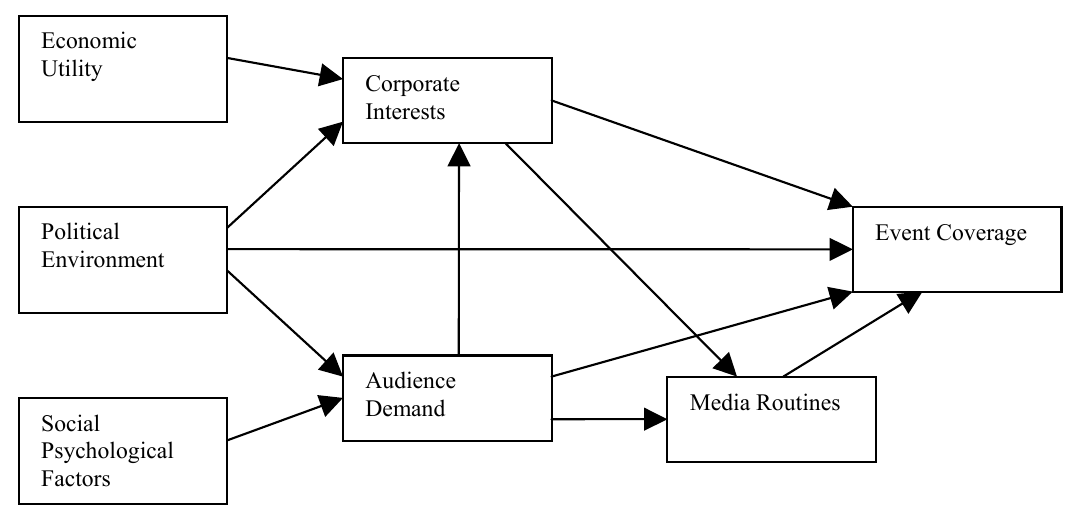
\includegraphics[scale=0.3]{img/2.2_modeloSesgo.png}
\par\bigskip
\small Fuente: \citep[8]{2005_Ortiz_NewspaperData}
\end{minipage}\bigskip


Concluyen que los datos empíricos\footnote{Donde se observan variaciones en el tipo de movimientos publicados, áreas de cobertura, cantidad de eventos reportados y ``patrones de cambios en protestas''; que pueden ser explicados por modificaciones en factores de selección del medio (en lugar de cambios propios de la protesta social).} soportan en mayor medida la inestabilidad inherente en los eventos reportados. Considerando además a los ciclos de atención mediática que (por su volatilidad) no son fácilmente anticipables y al desarrollo de nuevas tecnologías que cambian la dinámica de los medios, asumen que las estrategias para corregir ---o ignorar--- los sesgos no son lo suficientemente confiables.



\subsubsection{Línea editorial}
\label{sec:Sesgo_lineaEditorial}

Uno de los factores que merece una mención aparte por su relevancia en la cobertura y selectividad de los movimientos reportados es la línea editorial. 
Según \citet{2014_Hutter_AEP} varios estudios indican que medios liberales o de izquierda radical son menos selectivos que medios conservadores. 
Y \citet{1999_OliverMyers_LocalNewspapers} sugieren que los medios liberales favorecen especialmente mítines y eventos patrocinados por organizaciones de los movimientos sociales o grupos recreacionales.

De acuerdo a la perspectiva de la esfera pública, la selección de un diario particular en el AEP puede estar asociada en mayor medida a su importancia y línea editorial, pues esto define fuertemente su representación como un espacio público \emph{diferente}, \emph{importante} e \emph{influyente}:

\begin{center}
    \begin{minipage}{0.9\linewidth}
        {\setlength{\parindent}{12pt}\small
          Por diferente queremos decir que los lectores del periódico deberían ser diferentes en términos de su posición política en una sociedad determinada. 
          Por importante queremos decir que el espacio público representado por un periódico debe ser significativamente grande, lo que se puede medir por el número de ejemplares en circulación. 
          No tiene mucho sentido usar periódicos que pocas personas leen. 
          Por influyente, nos referimos a periódicos leídos por personas en posiciones influyentes en la configuración de políticas públicas (elites políticas, económicas e intelectuales). \normalsize \citep[117]{2003_Wada_Tesis}.
        }
    \end{minipage}
\end{center}

En síntesis, si un medio cumple en gran medida estas tres características, puede mostrarnos un punto de vista vinculado a grupos preponderantes, donde se postula una visión característica de la realidad, definida en el diario por su línea editorial.



\subsubsection{La labor del reportero}
\label{sec:Sesgo_reportero}

Entendemos al reportero como un actor social, que de acuerdo a pautas éticas y estándares profesionales construye el relato descriptivo de un evento, enfatizando u omitiendo elementos relevantes de una noticia. 
Según el control editorial que un medio pueda ejercer sobre este primer relato, se debe ponderar que ``la labor de los periodistas que cubren la protesta o marcha responde a los intereses de quienes los contratan'' \citep[278]{2015_Nicolasa_MassMedia}. 
Consideramos además que podemos obtener una mejor comprensión del sesgo introducido por su actividad profesional a partir de la relación que los medios pueden tener con los movimientos sociales; ya que su relación directa puede resultar áspera:

\begin{center}
    \begin{minipage}{0.9\linewidth}
        {\setlength{\parindent}{12pt}\small
          El tratamiento mediático de las protestas suele generar una indignación creciente entre los activistas, que ven deformada su aparición pública. 
          Entonces, la respuesta de ``ataque'' (...) a los medios cobra la forma de agresiones e insultos contra periodistas y camarógrafos.
          
          (...)
          
          La paradoja es que, por un lado, el movimiento quiere visibilizarse, exige presencia mediática; pero, por otro, detesta, desconfía y confunde a los enviados de los medios. 
          Muchos periodistas acaban siendo víctimas de agresiones e insultos por parte de los manifestantes y a la vez sufren la represión o la agresión policial. 
          La dificultad para cubrir protestas sociales que enfrentan los reporteros hoy, principalmente camarógrafos y fotógrafos, va en perjuicio de la audiencia y del propio movimiento: no sólo tienen problemas para conseguir la información que les permitiría hacer sus notas, sino que encuentran poca motivación para buscar fuentes del movimiento o recabar testimonios. 
          Además corre riesgo su integridad física ante la indistinción que hace la policía a la hora de reprimir.
          \normalsize \citep[43--44]{2013_Rovira_ActivismoMediatico}.
        }
    \end{minipage}
\end{center}




\subsubsection{Plataforma de difusión}
\label{sec:Sesgo_plataforma}

Como estrategia para comercializar su contenido, distintos medios periodísticos han optado por mantener una versión en línea de forma paralela a su versión impresa\footnote{Mención aparte merecen los medios nativos digitales, que no tienen un soporte en papel; sin embargo, no son considerados en este trabajo ya que en México su contenido favorece al periodismo de opinión o de investigación antes que al reportaje sobre protestas.}. 
La forma, validez, alcance, importancia, permanencia y renovación de los contenidos puede variar en distinta medida dependiendo de la plataforma de difusión utilizada. 
\citet{2006_Albornoz_PeriodismoDigital} indica como alguna de las principales diferenciaciones en plataformas digitales la capacidad para almacenar una gran cantidad de textos y actualizar noticias en tiempo real\footnote{Como ejemplo de esto, el diario \emph{El Universal} indica que se actualizan sus secciones principales ``Minuto x Minuto'' recibiendo la visita diaria de cerca de 150 mil usuarios únicos que ven más de 5 millones de páginas por día ---Consultado en \url{http://archivo.eluniversal.com.mx/disenio/directorios/historia_frame.htm}, el 27 de noviembre de 2017---.}, de modo que se ha reconocido que ``el nuevo medio está vivo y si en su nacimiento adoptó los géneros del periodismo escrito, en muy poco tiempo ha generado lenguajes y géneros periodísticos propios'' \citep[12]{2011_Valcarce_ciberperiodismo}. 
Entender la plataforma digital también nos habla de nuevas rutinas adoptadas y la dirección en la que se mueve el periodismo, pues la menor circulación de periódicos en Estados Unidos y Europa ``ha llevado a no pocos expertos a predecir la muerte del diarismo impreso'' \citep[53]{2008_ASF_Medios}.

Desde los soportes digitales se ha promovido el incremento en la producción de noticias, haciendo urgente la necesidad de establecer criterios adecuados para la selección de fuentes confiables ya que ``la dura competencia entre los medios periodísticos potencia hasta extremos peligrosos uno de los valores más apreciados por el periodismo: la velocidad. Cada vez más deprisa parece ser la consigna'' \citep[20]{2011_Valcarce_ciberperiodismo}. 
Cada vez menos confiable, puede ser el corolario derivado de la sobreabundancia informativa, referida coloquialmente como ``información chatarra'' dada la inmediatez y frivolidad que su consumo puede implicar.

La forma en la que se sostienen económicamente algunas plataformas puede influir también en la calidad de sus reportajes, en particular para periódicos digitales que no generan ingresos por la lectura de sus textos, se dice que ``el medio antes vendía información a sus lectores, mientras que hoy vende lectores a sus anunciantes. Por tanto, la información se da gratuita. Y si la voy a regalar, ¿por qué la voy a pagar cara? Entonces pagaré menos a mis periodistas, gastaré menos en investigar''\footnote{Ignacio Ramonet, en una reflexión realizada en Blanco y Negro Dominical el 15 de abril de 2011}.




\subsection{Sesgo asociado a los protocolos de búsqueda}
\label{sec:Sesgo_protocolo_busqueda}

En la sección \ref{sec:AEP_MuestreoTextos} hablamos sobre distintos tipos de búsqueda, aquí evaluamos sus principales deficiencias. En su forma más preocupante, se puede considerar que ``cada fuente y estrategia de búsqueda identifica un subconjunto diferente de eventos que producen diferentes perspectivas de \emph{lo que sucedió}'' \citep[132]{2001_Maney_Oliver__FindingEvents}.

Dada la enorme cantidad de textos disponibles en nuestras fuentes, la selección de textos específicos de interés para la investigación constituye por sí misma una forma de muestreo no probabilístico; usualmente dirigidos por la intuición, experiencia o conveniencia, estos métodos no suelen ser evaluados\footnote{Es importante considerar además que las estrategias de búsqueda pueden ser combinadas o modificadas en el transcurso de la investigación, de modo que su valoración puede resultar aún más complicada de realizar.} y ``se ejercen como prerrogativa del investigador. Además de la representatividad, un método de muestreo debe evaluarse en términos de si elimina o no el potencial de dicho sesgo de selección'' \citep[5]{2015_Lacy_BestContentAnalysis}.


\subsubsection{Búsqueda de texto completo}
\label{sec:sesgoMuestreo_full}

En fuentes impresas y digitales, la búsqueda de noticias por la lectura particular puede resultar una de las formas menos transparentes para extraer contenido. 
Se requiere de una gran atención, a menudo un evento de protesta puede ser referido sólo como un elemento adicional de una noticia más grande y sus características ser reflejadas exclusivamente en un pie de foto, en una fotografía, en un párrafo, en secciones del diario tan inverosímiles como ``deportes'', ``cultura'' u ``opinión''. 
Como señalan Maney \& Oliver: ``cualquiera que haya pasado horas con los ojos nublados leyendo periódicos en microfilmes entiende que la fatiga y el aburrimiento disminuyen el rendimiento humano'' \citep[136]{2001_Maney_Oliver__FindingEvents}.

Como consecuencia, \citet{2001_Maney_Oliver__FindingEvents} describen que los resultados generados por este tipo de búsqueda captan de manera desproporcionada eventos grandes y centrales para el diario; es decir, aquellos que se resaltan más por su carácter estético.

\subsubsection{Búsqueda por palabras clave}
\label{sec:sesgoMuestreo_keywords}

El muestreo por términos analíticamente relevantes no ofrece a todos los eventos de protesta la misma probabilidad de ser muestreados: la noticia que reporte el evento debe tener alguno de los términos o no será considerada. 
Crear una lista de palabras que se utilizarán para la búsqueda de protestas conlleva un protocolo propio, que implica mantener un balance entre la \emph{validez} y la \emph{ineficiencia} de cada término añadido. 
Donde la validez de un término de búsqueda es cuantificada a través de la detección de eventos de protesta relevantes, que no han podido ser captados por otros términos y la ineficiencia es medida por el número de notas periodísticas detectadas, no relevantes para los eventos de protesta ---falsos positivos---. 
Por lo que ``el investigador debe ser muy tacaño con respecto a renunciar voluntariamente a la validez y, posteriormente, estar dispuesto a tolerar la ineficiencia en la medida en que lo exija'' \citep[78]{2010_Strawn_keywordSearch}.


Los resultados que se derivan de esta técnica, ya sea que se utilicen términos generales o específicos, terminan siendo altamente consistentes. Como afirma Strawn para su protocolo, basado en descriptores generales de eventos en español: 
``los resultados sugieren que este protocolo genera datos con un alto grado de validez de búsqueda con respecto a la localización de reportajes de formas convencionales de eventos de protesta, pero es problemático con respecto a la identificación de formas de protesta no convencionales'' \citep[69]{2010_Strawn_keywordSearch}. 


Finalmente, el motor de búsqueda utilizado para localizar textos por palabras clave también afecta los resultados devueltos. Ya que los avances en el procesamiento del lenguaje natural han permitido importantes mejoras, la mayoría de los buscadores actuales \emph{lematizan}\footnote{
La lematización de una palabra modifica un término a una forma base ---denominada \emph{lema}---, de modo que no se centra en tiempos verbales o conjugaciones, sino que hace referencia a su raíz semántica, lo que permite agilizar la búsqueda. Por ejemplo: \emph{pienso}, \emph{pensó} y \emph{pensamos} son términos que pueden ser reducidos a 	\emph{pensar}.}
o realizan \emph{stemming}\footnote{
Aunque a veces se confunde con la lematización ---si bien, puede ser complementado con esta---, el stemming es otra técnica lingüística que también busca reducir la variedad de un término, pero está basada en algoritmos que modifican el prefijo o sufijo de una palabra para obtener una forma más simple ---o \emph{stem}---. Por ejemplo: \emph{familiar}, \emph{familia} y \emph{familiares} pueden ser reducidos a \emph{famili}. Esta técnica es particularmente ineficiente para verbos irregulares.}
a los términos introducidos, eliminan las \emph{palabras vacías}\footnote{
Una palabra vacía es un término que no tiene una fuerte carga semántica asociada, como \emph{el}, \emph{por}, \emph{ello}, \emph{ahi} o \emph{de}. Son además las palabras de mayor uso en un lenguaje, de modo que aparecen en casi cualquier texto, por lo que difícilmente aporta algo relevante a la búsqueda.}
 y otros más permiten la utilización de \emph{operadores booleanos}\footnote{
Como \emph{AND}, \emph{OR}, \emph{NOT} y otros. Google es más reconocido por permitir este tipo de operadores.},
que mejoran la búsqueda a través de la exclusión o incorporación combinada de múltiples términos. Sin embargo, casi ningún buscador comercial de Internet explica detalladamente el funcionamiento de los mismos; por lo que se deben usar con cautela, realizar pruebas y evaluar la consistencia de los resultados.



\subsubsection{Muestreos por exclusión}
\label{sec:sesgoMuestreo_temporal}

Algunos métodos de extracción de contenido están basados en la discriminación a priori de noticias periodísticas o algunos de sus elementos, lo cual facilita y reduce el trabajo de búsqueda.

Una de las técnicas más utilizadas en investigaciones históricas es el muestreo temporal, donde sólo se capta aquello que está dentro del marco temporal electivo. 
Sin embargo, incluso al aleatorizar periodos de búsqueda la probabilidad de selección es asimétrica y ``no sólo se truncan los ciclos de protesta, sino que también se pierden eventos dentro de disputas (o campañas colectivas), lo que altera fundamentalmente la proporción de acciones colectivas'' ---Strawn, en \citep[130]{2003_Wada_Tesis}---. 
Una forma de controlar hasta cierto punto este sesgo es a través de los patrones estacionales observados por investigaciones anteriores, donde acontecimientos importantes para nuestro estudio se pueden reproducir con mayor probabilidad\footnote{
Por ejemplo, \citet{2003_Wada_Tesis} buscó noticias cuatro semanas alrededor de las elecciones federales en México, celebradas cada 3 años para identificar patrones de cambio histórico; basado en la oportunidad política que el evento implica. Y \citet{2002_Koopmans_AEP} muestrean los diarios de  cada lunes con el objetivo de captar protestas ocurridas el fin de semana; reconociendo que se otorga una subrepresentación a trabajadores y estudiantes, que tienden a protestar más entre semana.}.

Bajo una forma de muestreo por conveniencia se pueden excluir secciones de un diario donde se considera que es inusual detectar noticias relevantes. Dependiendo del tipo de exclusión, es posible que la pérdida sea más grave; las secciones más utilizadas suelen ser: \emph{política}, \emph{sociedad}, \emph{nacional} o \emph{local}. 
Y aunque es poco probable que en secciones \emph{culturales}, \emph{deportivas} o \emph{recreacionales} de un diario se encuentren noticias relacionadas a protestas, estas tienen una repercusión contextual específica de acuerdo a dichas categorizaciones\footnote{Para ejemplos específicos, se puede usar el siguiente query de búsqueda en Google:\\ \emph{inurl:cultura AND  site:jornada.unam.mx AND protesta}. Donde existe una precaución adicional: hemos detectado que los diarios en versiones electrónicas a menudo no indizan adecuadamente su contenido por sección, de modo que existen pérdidas aleatorias derivadas del mal manejo de las plataformas digitales.}.

Discriminar elementos de una noticia para facilitar la tarea de búsqueda es otra forma de excluir contenido. 
Por ejemplo, \citet{2015_Danilova_Linguistic} usa esta técnica, centrándose solo en los titulares de prensa. 
Sin embargo, como en el caso de búsquedas de texto completo, este protocolo implica pérdida de noticias donde las protestas no son tratadas como tema principal del texto.



\subsection{Errores de captura}
\label{sec:Sesgo_captura}

Los capturistas se sitúan entre los esquemas de codificación y el análisis de los datos recabados. 
Como sugiere Franzosi: ``La codificación no es para todos. El trabajo repetitivo que requiere atención cuidadosa e inteligencia no van de la mano. Considera capacitar a 10 capturistas y, si tienes suerte, puedes terminar con 5'' \citep[149]{2010_Franzosi_QNA}.

Aún suponiendo que el esquema de codificación sea lo suficientemente simple, estable y documentado; y que se brinde suficiente atención a los capturistas para que ejerzan un trabajo de calidad\footnote{Mediante capacitaciones, reuniones, resolución de dudas de captura y controles de calidad.}, la captura de la información pierde efectividad al procesar múltiples registros de forma consecutiva. 
Aunque interesante para individuos que tienen un perfil adecuado\footnote{Y es por ello que varios estudios emplean para este tipo de tareas a estudiantes de ciencias sociales.}, la captura de información se puede tornar repetitiva y aburrida.

Falta de especificación, ausencia o equivocación en el llenado de campos constituyen en este sentido errores aleatorios no intencionados que pueden ser mermados a través de una organización eficaz del proceso de captura y del desarrollo de herramientas informáticas que validen la consistencia de la información introducida. 
Como proponen \citet{2002_Koopmans_AEP}, ya que usualmente se requiere de un equipo de más de un par de personas y debido a que estas pueden tener una gran rotación en un proyecto grande, se debe contar con una infraestructura adecuada para almacenar, evaluar y hacer pruebas de comparabilidad entre capturistas.



\subsection{Errores de interpretación}
\label{sec:Sesgo_procesamiento}

Aunque varios investigadores se han esforzado hacer comparables los datos ``de'' y ``entre'' capturistas, implementando controles de calidad, revisiones de datos y capacitaciones exhaustivas; confiando en que después de tomar estas precauciones se puede asegurar cierta consistencia en los datos. 
Se ha considerado que los fallos de interpretación son inevitables para todas las categorías\footnote{Aunque, entre más abstracta sea la categoría, se reconoce un incremento en la preocupación que genera su interpretación.}. 
Shapiro y Markoff ---según \citep[144]{2003_Wada_Tesis}--- consideran a los capturistas como un ``instrumento de caja negra'' y Franzosi califica de ``mito'' la comparabilidad entre capturistas:

\begin{center}
    \begin{minipage}{0.9\linewidth}
        {\setlength{\parindent}{12pt}\small
        En el análisis de contenido, por mucho que los investigadores intenten reducir la discreción de los capturistas que introducen el texto en categorías abstractas a través de reglas de codificación escritas, las categorías abstractas de codificación resultan invariablemente en la contaminación del instrumento de medida. Los capturistas juegan al ``científico sustituto''. \normalsize \citep[36]{2010_Franzosi_QNA}.
        }
    \end{minipage}
\end{center}


\begin{center}
    \begin{minipage}{0.9\linewidth}
        {\setlength{\parindent}{12pt}\small
        Nuestra capacidad para entender incluso los textos más simples depende tanto del conocimiento contextual como de un conocimiento más amplio del ``mundo'' ---sin mencionar el conocimiento necesario para leer textos específicos, un código o marco de referencia--- que va más allá de lo que manuales de captura o sesiones de capacitación pueden lograr. (...)
        \\
        
        Uno de maestros de la retórica del Renacimiento,  Erasmo de Rotterdam, en su \emph{Copia: Fundations of the Abundant Style}, publicado por primera vez en 1512, un libro de texto retórico inmensamente popular, ilustra 147 variaciones de la oración ``su carta me complace mucho'' (\emph{tuae litterae me magnopere delecttarunt}). 
        Y si eso es cierto para una oración simple de solo cinco palabras, dejo a su imaginación pensar cuántas maneras hay para que los capturistas interpreten, analicen y asignen los diversos elementos textuales de las múltiples oraciones que componen una historia a las categorías. \normalsize \citep[148]{2010_Franzosi_QNA}.
        }
    \end{minipage}
\end{center}

Lo cual ha llevado a la implementación de categorías basadas en los textos y no en los intereses específicos de cada investigación. 
Sin embargo, esta variación reciente del análisis de contenido puede sugerir sólo otra forma de homogeneizar clasificaciones, donde se puede solicitar a los capturistas, por ejemplo, ``realizar tareas semánticas usando su competencia del lenguaje natural para encontrar sujetos, objetos, verbos y modificadores'' \citet[158]{2003_Wada_Tesis}. 
De modo que cualquier esquema de categorización debería probar su confiabilidad mediante pruebas de diagnóstico y superar sus deficiencias reduciendo la complejidad de sus clasificaciones.



\subsection{Problemas en los esquemas de codificación}
\label{sec:esquemas_de_codificacion}

Como mencionamos antes, errores sistemáticos de los capturistas son causados por la interpretación que cada individuo realiza de los esquemas de codificación y de los textos que convierte en categorías. 
Este problema está vinculado a la \emph{confiabilidad} de los datos, la cual usualmente toma dos formas según \citet{2015_Lacy_BestContentAnalysis} y \citet{2002_Koopmans_AEP}: \emph{confiabilidad de intracodificador} ---coherencia de un capturista a lo largo del tiempo--- y \emph{confiabilidad de intercodificador} ---coherencia entre los capturistas---. 
Ya que es un tema de interés para proyectos que utilizan alguna forma de análisis de contenido, dado que puede poner en entredicho la reproducibilidad de los resultados, se han propuesto distintas métricas para calcular estas confiabilidades. 
Sin embargo: 

\begin{center}
    \begin{minipage}{0.9\linewidth}
        {\setlength{\parindent}{12pt}\small
        Aunque es fácil pensar en la confiabilidad como una propiedad de o entre los capturistas, es importante recordar que el objetivo principal de las comprobaciones de confiabilidad de intracodificador e intercodificador es probar la confiabilidad \emph{del protocolo de codificación} y la capacidad del protocolo para dar como resultado una categorización de contenido consistente. \normalsize \citep[10]{2015_Lacy_BestContentAnalysis}.
        }
    \end{minipage}
\end{center}


Si los datos no son comparables entre capturistas, pese a los esfuerzos realizados para aumentar la confiabilidad, el fallo será responsabilidad del esquema de codificación, no de los capturistas; por lo que este debería ser revisado y modificado. Al respecto, se considera que entre más abstracta sea una categoría, peores datos producirá:

\begin{center}
    \begin{minipage}{0.9\linewidth}
        {\setlength{\parindent}{12pt}\small
        cuanto más abstracta sea la clasificación, y cuanto mayor sea el juicio que requiera, peor será la clasificación. 
        Una clasificación mala tiene múltiples desventajas. 
        No es confiable, sus resultados a menudo son imprecisos, y coloca las decisiones analíticas cruciales en manos de capturistas en lugar de en las manos de aquellos que realmente llevarán a cabo el análisis (Tilly, 1981, p.75). \normalsize Citado en \citep[145]{2003_Wada_Tesis}.
        }
    \end{minipage}
\end{center}


Adicionalmente, cambios abruptos en las categorías pueden hacer incomparables los datos producidos entre un esquema y otro, por lo que se debe realizar un cuidadoso diseño de la investigación desde el inicio de la misma, planteando con exactitud el tipo de preguntas que se desean contestar\footnote{
    Por ejemplo, Tilly indica que ``la búsqueda de regularidades internas, como secuencias recurrentes o vínculos causales entre eventos aparentemente separados, requieren catálogos de eventos más sofisticados que los recuentos simples que a menudo han caracterizado los análisis de eventos políticos'' \citep[252]{2002_Tilly_EventCatalogsAsTheories}. 
}. 
Es por ello que \citet{2002_Koopmans_AEP} sugieren realizar un periodo de prueba, para evaluar la eficiencia de los procedimientos ---y esquemas de codificación--- adoptados. 


Consideramos además que reducir la variedad lingüística de un texto por medio de clasificaciones estrechas produce pérdida de información sobre el evento, ya sea por deficiencias en los esquemas de codificación adoptados o por la exclusión a priori de información que no resulta de interés para la investigación. 
Como sugiere \citet{2010_Franzosi_QNA}, aunque estos esquemas recaben información de interés de múltiples variables sobre un evento, son principalmente diseñados para responder las preguntas de investigación planteadas (usualmente orientadas sólo al conteo de eventos o características de los mismos) de modo que su uso puede ser limitado para el análisis estadístico más general.

\begin{center}
    \begin{minipage}{0.9\linewidth}
        {\setlength{\parindent}{12pt}\small
        Janis (1980, p. 155) ya había preguntado: ``Supongamos que hemos probado la confiabilidad de una técnica de análisis de contenido.... Entonces surge la pregunta: \emph{¿Qué describen los resultados del análisis de contenido?}'' ¿Tus resultados empíricos realmente abordan tus construcciones teóricas? ¿Es el sesgo de los medios lo que tocan tus categorías de codificación o es otra cosa? \normalsize \citep[151]{2010_Franzosi_QNA}.
        }
    \end{minipage}
\end{center}







\section{Evaluación de los datos}
\label{sec:validezLAOMS}

Se ha puesto énfasis en describir la metodología del AEP y sus limitaciones debido a que no existe una evaluación significativa sobre los datos producidos por el LAOMS. 
Aunque el laboratorio ha reconocido (de forma especulativa) la existencia de sesgos provenientes del diario seleccionado, no se les ha dado importancia real. 
Sus procedimientos (aunque sustentados) no han sido discutidos más que superficialmente una vez establecidos, no se han contrastado con publicaciones recientes de especialistas en el método, se han conducido más por la intuición que por la evidencia y han sido modificados numerosas veces sin considerar sus implicaciones. 
El esquema de codificación cuenta con dos versiones\footnote{
    Con cambios relevantes entre una versión y otra. 
    Sin embargo, ambas versiones cuentan con una mayor cantidad de modificaciones sobre la medición de los campos. 
    Algunos de estos cambios (comprensibles) han sido motivados por observaciones emergentes en las protestas reportadas, otros (más preocupantes) obedecen a modificaciones sobre las mismas definiciones o interpretaciones dadas a los campos debido a situaciones no consideradas inicialmente.
} 
lo cual hace incomparables ciertas categorías; donde el actual esquema simplifica o elimina clasificaciones de la primer versión, dada la inconsistencia de información que es posible captar de la fuente. 
Las clasificaciones actuales para medir características de las protestas sirven sobre todo para hacer recuentos simples. Hasta el periodo considerado han colaborado como capturistas 45 personas en el proyecto (principalmente estudiantes de ciencias sociales, algunos comprometidos con la investigación y otros cuyo trabajo tuvo que ser repetido dado su pésimo desempeño) cuya permanencia usual no es mayor a un año. 
Finalmente, se han realizado controles de calidad como actividad extraordinaria y principalmente para la elaboración de informes, pero no se han calculado índices sobre la confiabilidad de y entre capturistas.


Desde luego, no subestimamos el cuidadoso trabajo que se desarrolla en el LAOMS\footnote{
Que ha reunido a algunos de los mejores investigadores sociales relacionados con el tema y que representa un caso único al adoptar el AEP para el estudio de movimientos sociales contemporáneos nacionales.}, y si hablamos con cierta dureza sobre el mismo, nuestro objetivo no es, de ninguna forma, rebajar sus méritos.
A pesar de todo, su base de datos es ``una de las más amplias y detalladas fuentes de información acerca de los tiempos de ocurrencia de acciones colectivas; el tipo de organizaciones o agrupaciones que participan; las temáticas que detonan la movilización, así como el tipo de demandas que se enarbolan por parte de quienes irrumpen en el espacio público para la expresión de algún agravio o insatisfacción social'' \citep[1]{2017_Urbina_estudiantes}. 
Reconocemos que realizar un análisis que demuestre más allá de toda duda razonable la selectividad, confiabilidad, verificabilidad, comparabilidad, limitación e inclusividad de los datos va más allá de los esfuerzos que este trabajo puede realizar. 
Sin embargo, nuestra intención es simplemente analizar fuentes, métodos y protocolos bajo las consideraciones planteadas en las dos secciones anteriores para acercarnos a la dirección y magnitud de estos problemas, de modo que se reconozcan las propias limitaciones de este trabajo.





\subsection{Los medios periodísticos en México}
\label{sec:Mediosnacionales}

Partiendo del evento de protesta como unidad de análisis definida por el LAOMS y tomando como fuente de información a la prensa escrita, consideramos la situación particular de este medio en México a fin de comprender el entorno al que se enfrenta nuestra propia fuente para reportar (o no) ciertos movimientos sociales. 
Como sugiere \citet{2008_Strawn_mediaValidity}, a pesar de que los diarios mexicanos operan bajo una economía de mercado, su cobertura periodística puede ser configurada más allá de sus líneas editoriales por dos vías singulares: (i) la intervención de actores gubernamentales y de otro tipo, quienes tratan de restringir la libertad de prensa a través de medios no institucionales y (ii) los factores sociales únicos que condicionan las protestas y los intereses periodísticos.


Históricamente, \citet{2003_Wada_Tesis} detecta cambios en la ``oportunidad de los medios'' (es decir, en la probabilidad de dar cobertura mediática a un evento de protesta, dada la naturaleza de las relaciones entre la élite y los medios) como consecuencia de la pérdida de poder del Partido Revolucionario Institucional (PRI), quien por décadas mantuvo un control casi absoluto sobre la industria:

\begin{center}
    \begin{minipage}{0.9\linewidth}
        {\setlength{\parindent}{12pt}\small
         La oportunidad de los medios mexicanos ha pasado por una lenta y gradual apertura del elitismo puro al elitismo institucional con pequeños espacios de pluralismo (...) Con la caída del control estatal, la prensa mexicana debe operar ahora con la lógica del mercado. \normalsize \citep[114---115]{2003_Wada_Tesis}.
        }
    \end{minipage}
\end{center}

A pesar de esta libertad obtenida, aún considerando los cambios en el régimen de gobierno y la implementación de nuevas políticas públicas, se ha afirmado que ``los medios se han adaptado muy bien a las nuevas disposiciones gubernamentales, demostrando que, ante todo, sirven a un poder que está por encima de los partidos políticos, el poder económico'' \citep[223]{2011_Tesis_LaJornada}. 
Por lo que su aversión al riesgo puede impulsar una mayor selectividad de contenidos, particularmente aquellos que sean más complacientes a sus lectores o anunciantes. En 1986, Fátima Fernández nos advertía:

\begin{center}
    \begin{minipage}{0.9\linewidth}
        {\setlength{\parindent}{12pt}\small
         Los periódicos diarios de la ciudad de México están respaldados, o por un grupo económico, o por un grupo político, que ejerce en cada diario una influencia particular de acuerdo al tipo de participación, que va desde la propiedad del periódico mismo, hasta la influencia ocasional en un conflicto determinado. \normalsize ---Fernández, F., citada en \citep[206]{2011_Tesis_LaJornada}---.
        }
    \end{minipage}
\end{center}

En la actualidad, \citet{2013_HuertaGomez_ConcentracionMedios} refieren que México cuenta con uno de los mercados de comunicación y telecomunicaciones más concentrados del mundo; lo cual reduce la pluralidad de las voces en la sociedad. 
A pesar de ello, en publicaciones impresas a partir del año 2000 se observa una tendencia a la diversidad, debido a que la competencia comercial sucede en prácticamente todas las ciudades de México\footnote{Aún cuando ``el mercado de las publicaciones impresas es más pequeño debido al alto índice de analfabetismo real y funcional'' \citep[117]{2013_HuertaGomez_ConcentracionMedios} lo que genera ``un país de muchos periódicos pero pocos lectores (...). Los diarios estables son algo más de 300. Sin embargo, no suman más de 50 los que se pueden considerar que tienen auténtica presencia pública, local o nacional.'' \citep[282]{2011_Tesis_LaJornada}.}. 
Sin embargo, más allá de esta diversidad, \citet{2013_Garcia_PrensaMex} refiere una gran centralización geográfica, identificando a la capital del país como su mercado más grande. También nos advierte que ningún medio de información general publicado en el centro del país puede ser considerado como prensa \emph{de circulación nacional}\footnote{
Sugiere, en su lugar el término ``prensa \emph{de referencia nacional}'', ya que caracteriza mejor la visión de este tipo de diarios.}, pese a su identificación común como tal\footnote{
Indica como ejemplo, que la Secretaría de Relaciones Exteriores (SRE) a través del Consulado General de México en San Diego enlista lo que considera periódicos de circulación nacional: \emph{El Economista}, \emph{La Jornada}, \emph{Diario de México}, \emph{El Financiero}, \emph{El Sol de México}, \emph{El Universal}, \emph{Esto}, \emph{Excélsior}, \emph{La Crónica}, \emph{La Prensa}, \emph{Milenio}, \emph{Reforma} y \emph{Unomásuno} \citep[80]{2013_Garcia_PrensaMex}.}; ya que ningún diario está disponible a lo largo y ancho del país\footnote{
Resulta curiosa la observación en este aspecto del diario \emph{La Jornada}, ya que los números que reporta en circulación en provincia ``resultan inverosímiles'' \citep[81]{2013_Garcia_PrensaMex}, aún cuando ``la prensa tiene tendencia a aumentar los datos de tirajes y circulación a fin de seducir a los anunciantes'' (p.69).} (motivo que según \citet{2005_Ortiz_NewspaperData} sesga el tipo de información publicada, ofreciendo mayores reportes de áreas donde el diario tiene una mayor presencia).

``En México es bien sabido que la prensa escrita difícilmente sobreviviría si dependiera nada más de las suscripciones y ventas'' \citep[227]{2011_Tesis_LaJornada} por lo que se debe tener en cuenta el papel fundamental de la publicidad comercial o gubernamental\footnote{
Se argumenta que ``el Estado mexicano es el creador de la prensa moderna, ya que sin su constante ayuda (léase dinero pagado por conceptos de publicidad oficial), la prensa no sobreviviría más allá de lo que le permitieran sus reservas de papel'' \citep[228]{2011_Tesis_LaJornada}.} para su solvencia. En particular, la publicidad oficial tiene la capacidad de estrechar la relación entre medios de comunicación y gobierno, poniendo en entredicho la independencia de un medio\footnote{
Un caso representativo se da en el diario \emph{Excélsior} ---ver \url{https://es.linkedin.com/pulse/excélsior-cómo-cobrar-millones-sin-vender-un-juan-carlos-romero-puga}--- y otro, en el caso del ex secretario de Comunicación Social del ex gobernador de	Sonora, Guillermo Padrés, quien fue denunciado y pasó once meses en prisión preventiva durante 2016 por delitos de extorsión a medios, al solicitar el pago de una cuota para liberar publicidad oficial ---ver \url{http://www.letraslibres.com/espana-mexico/revista/los-fiscales-estan-solos}---.} pues ``estas relaciones son un terreno fértil para la censura sutil y el desarrollo de redes de corrupción'' \citep[6]{2017_FUNDAR_PublicidadOficial}. 
En especial para medios reconocidos por la calidad de sus contenidos, puesto que su publicidad resulta más costosa:

\begin{center}
    \begin{minipage}{0.9\linewidth}
        {\setlength{\parindent}{12pt}\small
         por un lado, los periódicos ``serios'' aluden al mayor perfil socioeconómico en comparación con los lectores de periódicos deportivos o policíacos; por otro lado, buena parte de los ingresos por publicidad proviene de la propaganda gubernamental o de los partidos políticos, cuyas inserciones pagadas no se basan en la efectividad o impacto del medio, sino en la relación política que se desea tener con las publicaciones. 
         En otras palabras, la publicidad es costosa en periódicos que no cuentan con un amplio número de lectores, sino por una práctica de relación con el poder, el cual paga para que no le peguen o para comunicarse con un círculo socioeconómico alto o influyente. \normalsize \citep[133--134]{2013_HuertaGomez_ConcentracionMedios}.
        }
    \end{minipage}
\end{center}

\citet{2013_Garcia_PrensaMex} señala que la prensa impresa requiere urbanización, de manera que su circulación sea posible y de lectores que paguen por su producto, lo cual puede ser asociado ---sobre todo a la prensa que se ocupa de temas políticos--- a educación, urbanidad y bienestar general, que comprende capacidad económica, lo cual puede explicar la desproporción en las tasas de penetración del medio, restringidas sólo a ciertas áreas\footnote{
Tomando en consideración tasas de natalidad y de mortalidad de la prensa, considera que aunque la prensa en general goza de mayor estabilidad actualmente, el número de títulos y su circulación está en regresión. \citet{2011_Tesis_LaJornada} sugiere además que la competencia no es reñida, puesto que a pesar de que existe una gran cantidad de títulos, por lo general en cada capital estatal sólo existen uno o dos diarios líderes.}. 
Además, la distribución del tiraje puede ser crucial como método de control adicional, sobre todo en la capital del país donde \citet{2011_Tesis_LaJornada} señala el acaparamiento que realiza \emph{La Unión de Voceadores} como conexión entre los medios impresos y el público.


Otro aspecto relevante del contexto periodístico mexicano, es la alta tasa de denuncia al año de diferentes clases de intimidación, agresión psicológica y asesinato. 
Según el informe \emph{Libertad de prensa} publicado por \citet{2017_FreedomPress}, México tiene un puntaje negativo de 64 en una escala de 100, y se coloca en el lugar 139 de 199 países en libertad de medios (clasificando en una categoría donde se considera que casi no existe libertad de prensa), indicando además que: 

\begin{center}
    \begin{minipage}{0.9\linewidth}
        {\setlength{\parindent}{12pt}\small
        Brasil, Colombia, Honduras y México continúan siendo uno de los lugares más peligrosos para los periodistas en el mundo, y todos enfrentan retos continuos en la investigación y persecución de estos crímenes. 
        Según algunas fuentes, el número de asesinatos en México aumentó, especialmente para periodistas que cubrían abusos policiales, tráfico de drogas y corrupción gubernamental \normalsize \citep[21]{2017_FreedomPress}.
        }
    \end{minipage}
\end{center}


En términos generales, la prensa mexicana contemporánea puede ser referida como ``oligopólica, escandalosa, poco profesionalizada, sembrada de personalidades con enormes egos, partidista y profundamente vitriólica'' \citep[33--34]{2008_ASF_Medios} por lo que ``las noticias políticas, principal insumo de un periódico formal, adolecen de confianza en la percepción del público general debido a una historia de tradición epistolar entre el poder político y los periódicos'' \citep[131]{2013_HuertaGomez_ConcentracionMedios}. 
Ante tal panorama, resulta fácil adivinar una relación complicada con los movimientos sociales:

\begin{center}
    \begin{minipage}{0.9\linewidth}
        {\setlength{\parindent}{12pt}\small
         De acuerdo con Pablo Romo, de la organización civil Serapaz dedicada a dar seguimiento a la conflictividad social, los movimientos no existen en el vasto número de los medios de comunicación abiertos mexicanos, en especial las televisoras, pero identifica cuatro momentos de la estrategia con que son tratados: la invisibilidad, el achicamiento, la descalificación y, finalmente, la criminalización. \normalsize \citep[47]{2013_Rovira_ActivismoMediatico}.
        }
    \end{minipage}
\end{center}



\subsubsection{Variedad de medios digitales que reportan protestas}
\label{sec:Mediosnacionales_VariedadMedios}

Como primer cuestionamiento para establecer puntos de comparación más allá de la argumentación, vale la pena preguntarnos ¿cuántos diarios on-line\footnote{Se consideran sólo medios periodísticos digitales nacionales ya que la recolección de notas periodísticas por el LAOMS es realizada a través de este medio particular y debido a la facilidad que ofrece la extracción y el tratamiento de sus textos.} existen en México? 
Así, se contabilizaron los diarios digitales activos de carácter general\footnote{Es decir, no enfocados exclusivamente a un ámbito informativo no relevante para la protesta, como deportes, sociales o espectáculos.} que reportaron al menos un evento de protesta en formato HTML desde la creación del sitio y hasta el 9 de octubre de 2016, obteniendo 394 medios, de los cuales en 377 fue posible determinar su sede estatal\footnote{La mayor parte de ellos cuenta con versiones impresas distribuidas alrededor de la zona en la que han sido identificados, en otros casos es el propio diario el que refiere su estado de procedencia.}. 
La lista se construyó de acuerdo al Catálogo Nacional de Medios Impresos e Internet, \citet{2016_INE_catalogoMedios} y listas anteriores, disponibles en \url{http://kiosko.net/mx/}, \url{http://www.prensaescrita.com/america/mexico.php} y \url{http://www.alexa.com/} junto a algunas búsquedas propias simples. El listado por estado se agrupa en la tabla \ref{DiariosDigitales}.


\begin{table}[!hbt]
\center
\small
\caption{Medios periodísticos digitales nacionales por estado}
\label{DiariosDigitales}
\begin{tabular}{ | l | c || l | c || l | c | } 
\hline
Aguascalientes & 6 & Baja California & 8 & Baja california Sur & 3 \\
\hline
Campeche & 5 & Chiapas	& 21 & Chihuahua & 9\\
\hline
Ciudad de México & 19 & Coahuila & 14 & Colima & 2 \\
\hline
Durango & 8 & Guanajuato & 7 & Guerrero & 20\\
\hline
Hidalgo & 13 & Jalisco & 8 & México & 16 \\
\hline
Michoacán & 15 & Morelos & 10 & Nayarit & 9\\
\hline
Nuevo León & 6 & Oaxaca & 20 & Puebla & 13 \\
\hline
Querétaro & 7 & Quintana Roo & 12 & San Luis Potosí & 8\\
\hline
Sinaloa & 5 & Sonora & 16 & Tabasco & 13 \\
\hline
Tamaulipas & 28 & Tlaxcala & 2 & Veracruz & 42\\
\hline
Yucatán & 7 & Zacatecas & 5 & &\\
\hline
\end{tabular}
\par\bigskip
\caption*{\small Fuente: Elaboración propia}
\end{table}


\subsubsection{Cobertura parcial comparativa en los periódicos digitales más leídos}
\label{sec:Mediosnacionales_CoberturaComparativa}


Como método para acotar el listado de la tabla \ref{DiariosDigitales}, se considera el éxito que tiene un medio entre sus lectores\footnote{
Algo que es asociado por \citet{2003_Wada_Tesis} a la ``importancia'' de un medio.}, lo cual es medido a través del \emph{tráfico web}\footnote{Cantidad de datos enviados y recibidos por los visitantes de un sitio.} que cada sitio genera en México. 
Para realizar esta consulta se ha recurrido al sitio Web de Alexa\footnote{
Información consultada el 16 de octubre de 2016 en \url{http://www.alexa.com}.}, propiedad de \emph{Amazon}, donde se mide el tráfico en la Red usando filtros por categoría o por región. Bajo un algoritmo propio, el mismo sitio realiza algunas precisiones acerca de los datos que genera:

\begin{center}
    \begin{minipage}{0.9\linewidth}
        {\setlength{\parindent}{12pt}\small
	    Las estimaciones de tráfico de Alexa se basan en datos de nuestro panel de tráfico global, que es una muestra de millones de usuarios de Internet que utilizan una de las más de 25.000 extensiones de explorador diferentes. 
	    Además, recopilamos gran parte de nuestros datos de tráfico de fuentes directas en forma de sitios que han elegido instalar el script de Alexa en su sitio y certificar sus métricas. 
	    Sin embargo, los propietarios de sitios siempre pueden optar por mantener sus métricas certificadas privadas.
	    Nuestro rango de tráfico global es una medida de cómo un sitio web lo está haciendo en relación con todos los otros sitios en la web en los últimos 3 meses. 
	    El rango se calcula utilizando una metodología patentada que combina el promedio estimado de visitantes únicos diarios y su número estimado de páginas vistas durante los últimos 3 meses. 
	    Proporcionamos un ranking similar a un país específico, que es una medida de cómo un sitio web clasifica en un país en particular en relación con otros sitios en el último mes.  \normalsize \url{http://www.alexa.com/about}.
        }
    \end{minipage}
\end{center}

Del listado de los 500 sitios más consultados en México, sólo 47\footnote{Resulta curioso observar que \emph{La Jornada} no tiene asignado un ranking dentro del listado, suponemos que se debe a que su servidor no admite la medición del tráfico a través del método de Alexa. De cualquier modo, el reporte \citet{2016_INE_catalogoMedios} ofrece información adicional sobre el tráfico en su sitio.} corresponden a medios periodísticos nacionales considerados bajo nuestros anteriores criterios, los cuales son presentados en la tabla \ref{DiariosDigitales_rankeados}.


\begin{table}[!hbt]
\center
\caption{Medios periodísticos digitales rankeados en México por su tráfico}
\label{DiariosDigitales_rankeados}
\resizebox{\textwidth}{!}{
\begin{tabular}{ | l | l | l | c | l | l | c | l | } 
\hline
\textbf{Nombre} & \textbf{Sede} & \textbf{Sitio web} & \textbf{Ranking Alexa} & \textbf{Tipo} & \textbf{Tiraje}\protect\footnotemark & \textbf{Promedio de usuarios al mes} & \textbf{NSE}\protect\footnotemark \\
\hline
El Universal & Ciudad de México & www.eluniversal.com.mx & 19 & Nacional & 120,000 L-D & 15 millones de usuarios únicos & ABC+\\
\hline
Milenio & Ciudad de México & www.milenio.com & 34 & Nacional & 255,547 L-D (6 publicaciones) & 6.5 millones de usuarios únicos & ABC+CD\\
\hline
El Debate & Culiacán & www.debate.com.mx & 38 & Local & 68,500 L-D (5 publicaciones)& 2.4 millones de pageviews & C+C\\
\hline
El Siglo de Torreón & Torreón & www.elsiglodetorreon.com.mx & 40 & Local & 40,000 L-D &  &  ABCD\\
\hline
Excélsior & Ciudad de México & www.excelsior.com.mx & 49 & Nacional & 90,000 L-D & 6.8 millones de usuarios únicos &  ABC+\\
\hline
El Siglo &  & http://elsiglo.mx/ & 53 & Nacional & N/A &  & \\
\hline
Proceso & Ciudad de México & www.proceso.com.mx & 73 & Nacional & 93,692 Semanal & 24.3 millones pageviews & ABC+ y C\\
\hline
Aristegui Noticias & Ciudad de México & www.aristeguinoticias.com & 83 & Nacional & N/A &  & \\
\hline
Sin Embargo & Ciudad de México & www.sinembargo.mx & 84 & Nacional & N/A & 5.9 millones de visitas únicas & ABC+C\\
\hline
Televisa & Ciudad de México & www.televisa.com & 85 & Nacional & N/A & 15.7 millones de visitas & \\
\hline
SDP Noticias & Ciudad de México & www.sdpnoticias.com & 86 & Nacional & N/A & 13.2 millones de usuarios únicos & ABCD\\
\hline
Expansión & Periodico digital & www.expansion.mx & 96 & Nacional & 54,000 Catorcenal & 10 millones de visitas & ABC\\
\hline
Reforma & Ciudad de México & www.reforma.com & 100 & Nacional & 142,086 L-D & 2,393,130 usuarios únicos & ABC+\\
\hline
El Informador & Guadalajara & www.informador.com.mx & 119 & Local &  47,000 L-D & 1.7 millones de visitas & \\
\hline
Sipse & Yucatán & www.sipse.com & 139 & Local &  35,020 L-D & 5.4 millones de pageviews & \\
\hline
El Economista & Ciudad de México & www.eleconomista.com.mx & 150 & Nacional & 37,500 L-V & 710,466 visitas únicas & ABC+\\
\hline
Publimetro & Ciudad de México & www.publimetro.com.mx & 187 & Nacional & 260,000 L-V (3 publicaciones) & 3.5 millones de visitas únicas & ABC+\\
\hline
El Diario de Juárez & Ciudad Juárez & www.diario.mx & 200 & Local & 60,000 L-D & 2 millones de visitas & ABC\\
\hline
El Norte & Monterrey & www.elnorte.com & 225 & Local & 166,374 L-D & 489,520 visitas únicas & ABC\\
\hline
El Siglo de Durango & Durango & www.elsiglodedurango.com.mx & 246 & Local & 15,450 L-D &  &  AA+BC\\
\hline
Expreso & Hermosillo & www.expreso.com.mx & 266 & Local &  22,500 L-D & 2 millones de visitas &  ABC+\\
\hline
Animal Político & Ciudad de México & www.animalpolitico.com & 273 & Nacional & N/A & 3.8 millones de pageviews & ABC\\
\hline
El Imparcial & Hermosillo & www.elimparcial.com & 276 & Local &  40,287 L-D & 3.7 millones de visitas & \\
\hline
Vanguardia & Saltillo & www.vanguardia.com.mx & 283 & Local & 24500 & 5.2 millones de visitas & ABC\\
\hline
Radio Fórmula & Ciudad de México & www.radioformula.com.mx & 330 & Nacional & N/A &  & \\
\hline
El Gráfico & Ciudad de México & www.elgrafico.mx & 345 & Nacional & 300,000 L-D &  & ABCDE\\
\hline
La Crónica de Hoy & Ciudad de México & www.cronica.com.mx & 364 & Nacional & 76,000 L-D & 3 millones usuarios únicos & ABC\\
\hline
La Silla Rota & Ciudad de México & www.lasillarota.com & 373 & Nacional & N/A & 420,000 visitas &  ABC+\\
\hline
López Doriga & Ciudad de México & www.lopezdoriga.com & 375 & Nacional & N/A &  & \\
\hline
Zócalo & Saltillo & www.zocalo.com.mx & 376 & Local & 76,243 L-D (4 publicaciones) &  & ABCD\\
\hline
Frontera & Tijuana & www.frontera.info & 402 & Local & 50,000 L-D &  & ABC\\
\hline
Quadratín & Morelia & www.quadratin.com.mx & 407 & Local &  &  & \\
\hline
Diario de Yucatán & Mérida & www.yucatan.com.mx & 438 & Local & 54,000 L-D & 15 millones de pageviews & ABCDE\\
\hline
Nayarit en Línea & Nayarit & www.nayaritenlinea.mx & 453 & Local &  &  & \\
\hline
Noticias MVS & Ciudad de México & www.noticiasmvs.com & 471 & Nacional & N/A & 5.4 millones de visitas & \\
\hline
Pulso SLP & San Luis Potosí & www.pulsoslp.com.mx & 483 & Local & 27,000 L-D & 4.9 millones de pageviews & AB+B\\
\hline
24 Horas & Ciudad de México & www.24-horas.mx & 497 & Nacional & 112,000 L-V & 2.5 milliones pageviews & ABC+\\
\hline
La Jornada & Ciudad de México & www.jornada.unam.mx &  & Nacional & 110,236 L-D & 4.7 millones pageviews & ABC\\
\hline
\end{tabular}}
\par\bigskip
\caption*{\small Fuente: Elaboración propia, con datos del \citet{2016_INE_catalogoMedios} y Alexa.}
\end{table}
\addtocounter{footnote}{-1}
\footnotetext{Se indican los días en que se publica la versión impresa del medio; por ejemplo, L-V hace referencia a que la publicación es puesta en circulación de lunes a viernes. Algunos medios agrupan varias versiones locales publicadas en un mismo sitio web, en esos casos se hace la indicación de cuantos medios están agrupados (y el tiraje mostrado es calculado como la suma del tiraje individual de cada publicación).}
\addtocounter{footnote}{1}
\footnotetext{Se refiere al Nivel Socioeconómico asociado al perfil del lector. 
La primera letra del alfabeto contiene a la población con el más alto nivel de vida e ingresos del país, siguiendo el orden del alfabeto, la letra E representa a individuos de menores ingresos y nivel de vida en todo el país. 
Se consideran además modificadores como el signo + para hacer distinciones entre un estrato ligeramente superior a otro (por ejemplo, la población en A+ tiene un mejor nivel socioeconómico que la población en A).}


Considerar a los diarios más leídos, no implica que estos sean los más serios o de mayor calidad y puede ser incluso un criterio riesgoso para seleccionar una buena fuente de referencia; basta hacer notar que ---según información del propio \citet{2016_INE_catalogoMedios}--- el diario y la revista con mayor tiraje en el área metropolitana es \emph{El Gráfico} y \emph{TVyNotas} respectivamente, cuyo propósito es más recreativo que informativo. 
Sin embargo, medir la representación de la protesta en los diarios más leídos puede darnos una mejor visión sobre el tipo de contenidos publicados, su utilidad comparada y nos ofrece la posibilidad de detectar mejores fuentes, pues como anota Moreno de Alba:

\begin{center}
    \begin{minipage}{0.9\linewidth}
        {\setlength{\parindent}{12pt}\small
	    existen periódicos reconocidos como \emph{serios} por la gente que influye intelectualmente debido a múltiples factores, entre los que sobresale quizá el que prestan mayor espacio y atención a noticias y editoriales referentes a asuntos de interés público, ya sean nacionales, ya sean internacionales, de alguna manera trascendentes. 
	    A este tipo de publicaciones las denomino \emph{prestigiosas}.  \normalsize \citep[23]{1996_MorenoDeAlba_Prestigio}.
        }
    \end{minipage}
\end{center}




Utilizando los diarios de la tabla \ref{DiariosDigitales_rankeados}, palabras asociadas a los términos de búsqueda\footnote{
    Se incluyeron variaciones en tiempos verbales y conjugaciones donde se validó que el motor de búsqueda no obtenía resultados idénticos. 
    El protocolo de palabras clave fue creado a partir de palabras detectadas en los titulares de las noticias recuperadas por el LAOMS de \emph{La Jornada}.
} 
de la tabla \ref{TerminosBusquedaRegional} y la API de \emph{Google, Custom Search Engine} (\emph{CSE}) para python\footnote{
    Su documentación puede ser consultada en \url{https://developers.google.com/api-client-library/python/apis/customsearch/v1}.
} 
se obtuvieron 821 artículos periodísticos que contenían uno o más de los términos en sus titulares\footnote{
    Se recuperó la hipótesis de  \citet{2015_Danilova_Linguistic}, según la cual es posible extraer datos simples de eventos de protesta a partir de patrones genéricos encontrados en los titulares de prensa. 
    Por lo demás, éste método de muestreo hace más fácil y rápida la validación de contenido relevante dentro de una noticia. 
    El riesgo que implica es la pérdida de representatividad, ya que muchos de los encabezados en noticias que reportan protestas no contienen ninguno de los términos considerados.
} para marzo de 2016. 
Luego de comprobar la validez de los resultados\footnote{
    Es decir, que refirieron efectivamente eventos de protesta, ocurridos en territorio nacional para el mes muestreado, no reportados más de una vez en un día; donde además se cumplieran las condiciones específicas que \citet{2017_Cadena_ManualLAOMS} proponen para la identificación de la unidad de análisis de nuestro interés.
} su cantidad se redujo a sólo 371 registros, los cuales son presentados en la figura \ref{2.3_sesgoRegional} por la distribución estatal de los eventos referidos. 
Aunque no es concluyente, su cobertura comparada parece confirmar la centralidad regional de estos medios periodísticos y la gran heterogeneidad de la representación de la protesta en el país. 

\begin{table}
\center
\small
\caption{Términos de búsqueda usados para localizar eventos de protesta en diarios online}
\label{TerminosBusquedaRegional}
\begin{tabular}{ | l | l | l | l | } 
\hline
bloqueo & boicot & cadena humana & caravana \\
\hline
cierre de calles & cierre de vialidades & exigencia & huelga \\
\hline
manifestación & marcha & mitin & movilización \\
\hline
paro de labores & plantón & protesta & toma de edificios \\
\hline
\end{tabular}
\par\bigskip
\caption*{\small Fuente: Elaboración propia, a partir de textos recuperados por el LAOMS de \emph{La Jornada}.}
\end{table}


\hspace{-2em}\begin{minipage}{\linewidth}
\centering
\captionof{figure}{Distribución regional de protestas en medios periodísticos digitales (marzo 2016)} \label{2.3_sesgoRegional}
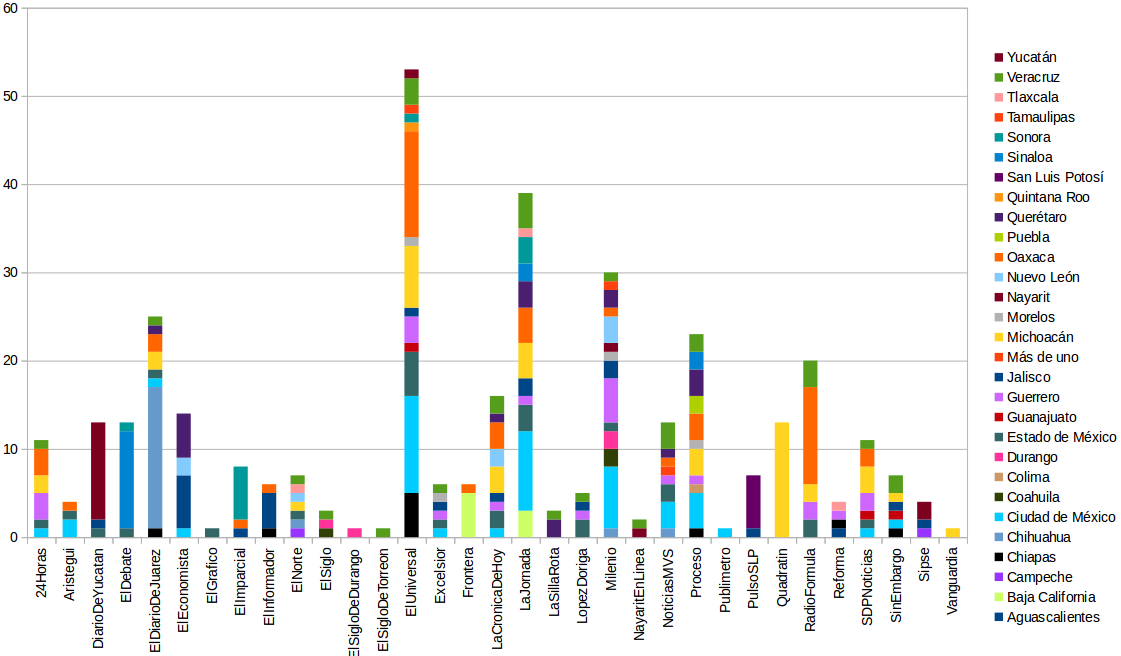
\includegraphics[scale=0.4]{img/2.3_sesgoRegional.png}
\par\bigskip
\small Fuente: Elaboración propia, con base en noticias detectadas en los medios referidos.
\end{minipage}\bigskip





\subsubsection{Otras coberturas comparadas}
\label{sec:Mediosnacionales_CoberturaComparativa2}

\citet{2005_Strawn_Tesis} consiguió dos reportes agregados de la Secretaría de Gobierno del Distrito Federal; al comparar dichos registros con reportajes sobre protestas\footnote{Donde su unidad de análisis es también el evento de protesta; sin embargo, su definición de tales eventos es más amplia, por lo que abarca una mayor cantidad de casos de los que considera el LAOMS.}, recolectados por él mismo para abril, mayo y noviembre de 2002 en los diarios \emph{El Norte}, \emph{Reforma} y la agencia \emph{Notimex} encontró un porcentaje de cobertura de 10\%, 25\% y 30\% respectivamente. 
Al ser datos agregados no se conoce a detalle la medición empleada por el gobierno para contabilizar protestas, pero Strawn confía (basando su especulación en las conversaciones que tuvo con aquellos que manejan los registros oficiales) que los criterios son muy parecidos a los suyos, de modo que las diferencias porcentuales pueden ser interpretadas como pérdida de información sobre protestas por muestreo en diarios. 
En la figura \ref{2.4_sesgo_oficial_vs_medios} se indica además como la tendencia a reportar manifestaciones con objetivos diferentes (en función de su alcance) difiere entre medios.

\begin{minipage}{\linewidth}
\centering
\captionof{figure}{Fuentes periodísticas vs fuentes oficiales* en el DF} \label{2.4_sesgo_oficial_vs_medios}
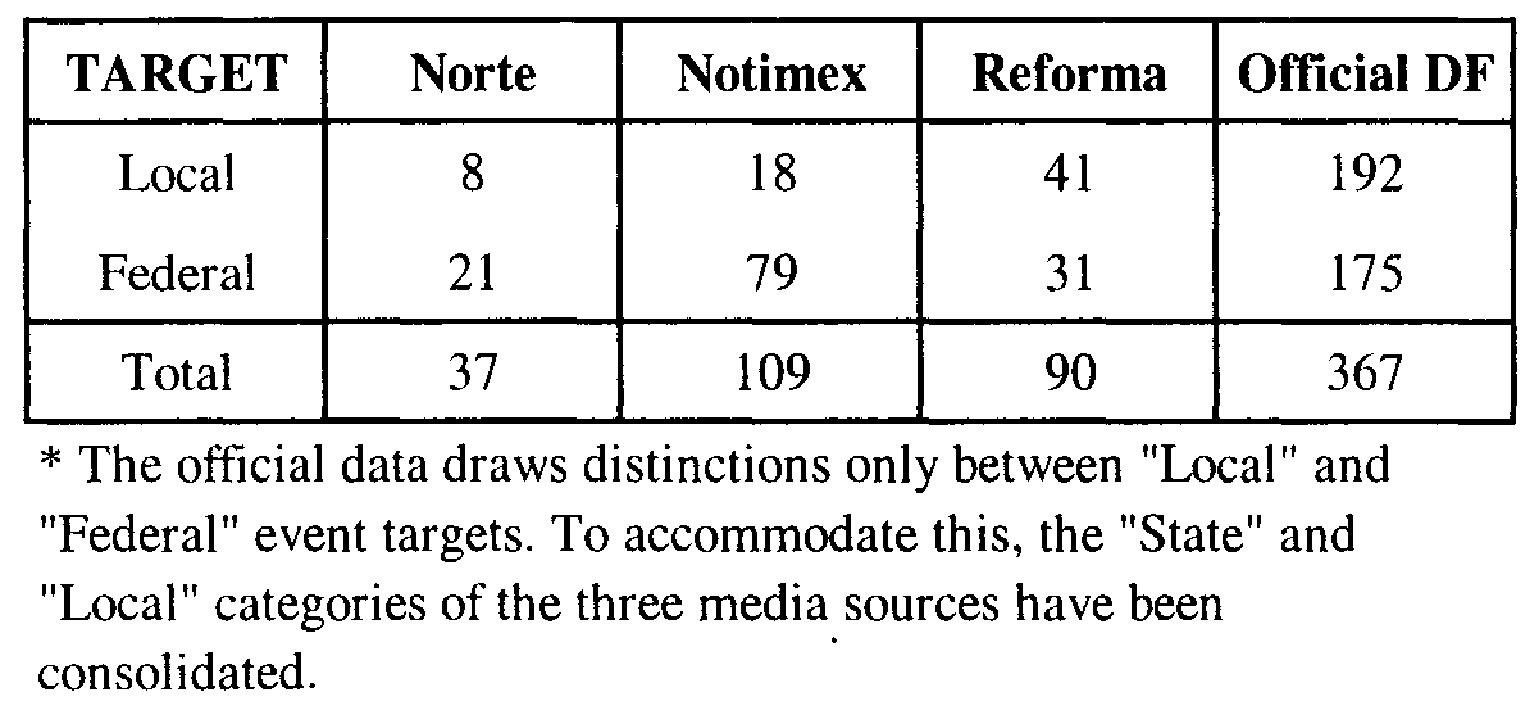
\includegraphics[scale=0.18]{img/2.4_sesgo_oficial_vs_medios.png}
\par\bigskip
\small Fuente: \citep[163]{2005_Strawn_Tesis}
\end{minipage}\bigskip


Además de esta comparación con fuentes oficiales, \citet{2008_Strawn_mediaValidity} comparó entre sí las muestras por diarios. 
De 710 eventos de protesta distintos identificados en todo el país, sólo 30 de ellos fueron reportados por las 3 fuentes y 84 de ellos por 2\footnote{Estos resultados son interesantes en función de la selección de las fuentes de referencia, ya que \emph{El Norte} y \emph{Reforma} pertenecen al mismo grupo editorial, esperaríamos una mayor cantidad de noticias duplicadas entre estos medios. 
Aún así, es posible que exista una mayor variedad entre medios pertenecientes a distintos grupos editoriales.}, existiendo 596 eventos reportados en una sola fuente, donde el 58.2\% de ellos provino sólo de \emph{Notimex}. 
Además, observó que son más frecuentes los reportes sobre protestas en los estados donde se publica la fuente que en ningún otro. Sólo se reportó el tamaño del evento de 1/2  a 1/3 aproximadamente del total (dependiendo de la fuente), favoreciendo a los eventos más grandes, con diferencias estadísticas significativas entre las medias. 
Respecto a los objetivos locales, una gran mayoría de protestas estuvieron centradas ---en las 3 fuentes--- en temas políticos, mientras que los objetivos nacionales están centrados en temas económicos; las variaciones en estos temas son mínimas, pero podrían ser significativas en una muestra más grande.


En el ámbito local, según un análisis de medios, a través de un sistema que contabiliza las apariciones de personajes e instituciones en los diarios impresos, realizado por \emph{La Jornada Aguascalientes} a medios regionales\footnote{La información básica del estudio, denominado ``Sistema Comparativo de Indicadores de Información'' (Sicoii) fue consultada el 03 de noviembre de 2017 en \url{http://www.lja.mx/2016/09/prevalece-sesgo-bipartidista-en-medios-comunicacion/}. 
Las mediciones consideran las apariciones en fotos de portada o titulares a ocho columnas, así como de notas interiores publicadas en los periódicos \emph{El Sol del Centro}, \emph{Hidrocálido}, \emph{El Heraldo de Aguascalientes}, \emph{Página 24} y \emph{La Jornada Aguascalientes}. 
El periodo estudiado abarca de mayo de 2015 a julio de 2016. Los actores considerados son el ayuntamiento capital, el gobierno del estado y sus respectivos titulares; los partidos políticos o sus dirigentes y los candidatos del PAN y del PRI a la gubernatura.}, previo a las elecciones estatales del 2016, se concluye que el bipartidismo ---información asociada al PRI o PAN--- acapara el 79\% de las portadas de los principales periódicos de Aguascalientes. 
Según sus propias palabras, este análisis pretende ``evidenciar la existencia de filias y fobias de los medios de comunicación hacia los personajes públicos, sus posicionamientos o sus institutos políticos; ya sea por afinidad emocional, apuesta política o contratación de espacios para la inserción de notas periodísticas''.




\subsubsection{Muestreo comparativo entre El Universal y La Jornada}
\label{sec:Mediosnacionales_Comparacion_UniversalJornada}


Por su importancia relativa, hacemos una comparación adicional entre los dos medios que ofrecen una mayor cobertura sobre protestas según la figura \ref{2.3_sesgoRegional}; es decir, \emph{La Jornada} y \emph{El Universal}. Los cuales mantienen a una gran cantidad de corresponsales en el país, son medios de gran tiraje e importancia y difieren ampliamente en sus líneas editoriales.

Para realizar esta comparación se utilizó de nuevo la API de Google \emph{CSE} \footnote{
    Y el protocolo de búsqueda descrito en la sección \ref{sec:NotiMuestreo} como \emph{búsqueda por keywords en CSE - versión 2}. 
} 
para el mes de abril de 2017\footnote{
    La selección de este periodo se realizó por conveniencia, ya que \emph{La Jornada} tiende a eliminar al poco tiempo las \emph{últimas noticias} que se publican exclusivamente en su sitio (aunque mantiene los artículos que se publican en su versión impresa). 
    Otro punto destacable de esta comparación es que El Universal publica casi exclusivamente ``información de último minuto'' (análoga a la que se presenta en \emph{últimas} para \emph{La Jornada}) sin que parezca existir gran control editorial en los reportajes, los cuales no se ajustan la mayor parte del tiempo a la versión impresa del diario.
}. 
Las búsquedas por palabras clave esta vez fueron más exhaustivas, localizando al menos uno de los términos referidos en los titulares, sumarios, pies de foto o cuerpo de la noticia.

También en este caso se validó que cada uno de los artículos tuviese al menos una referencia a un evento de protesta, no reportado ese mismo día y que fuese relevante de acuerdo a los criterios del LAOMS; etiquetando además el estado referido por la noticia. Se recuperaron 112 noticias de \emph{La Jornada} y 133 noticias de \emph{El Universal}. En la figura \ref{2.5_LaJornada_vs_ElUniversal} son comparados los conteos diarios, donde se comprueban pequeñas diferencias en la tendencia de los reportajes.

\hspace{-1em}\begin{minipage}{\linewidth}
\centering
\captionof{figure}{Comparación entre \emph{La Jornada} y \emph{El Universal} - Serie de tiempo diaria} \label{2.5_LaJornada_vs_ElUniversal}
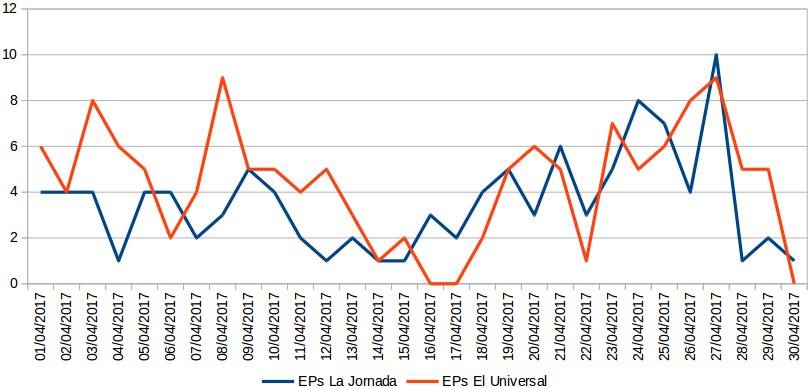
\includegraphics[scale=0.45]{img/2.5_LaJornada_vs_ElUniversal.png}
\par\bigskip
\small Fuente: Elaboración propia.
\end{minipage}\bigskip


Al hacer la comparación de cada una de estas noticias, se detectaron 34 eventos de protesta reportados por ambos medios. 
Es decir, \emph{El Universal} reporta 99 eventos que no son cubiertos por \emph{La Jornada}, quien a su vez reporta 72 eventos únicos. 
En cuanto a las diferencias regionales graficadas en la figura \ref{2.6_LaJornada_ElUniversal_estados}, se detectan discrepancias importantes de cobertura, donde suponemos que esto se debe sobre todo a una diferente distribución territorial en las redes de corresponsales y en las ediciones locales que ambos medios mantienen a lo largo de la república mexicana.


\begin{minipage}{\linewidth}
\centering
\captionof{figure}{Comparación entre \emph{La Jornada} y \emph{El Universal} - Estados referidos} \label{2.6_LaJornada_ElUniversal_estados}
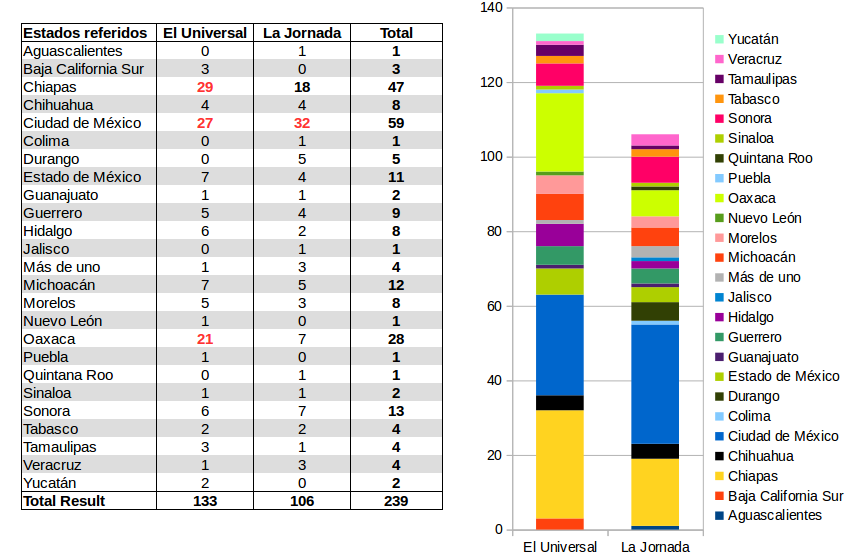
\includegraphics[scale=0.37]{img/2.6_LaJornada_ElUniversal_estados.png}
\par\bigskip
\small Fuente: Elaboración propia.
\end{minipage}\bigskip


Por último, tomamos en consideración la propia categorización que los medios hacen de su contenido en la figura \ref{2.7_LaJornada_ElUniversal_secciones}, donde se ubican importantes distinciones. 
Resulta interesante comprobar que ambos medios refieren una mayor cantidad de eventos de protesta bajo la sección de \emph{estados}, pero que \emph{La Jornada} presta una atención similar del tema en su sección de política, lo cual puede manifestar sus intereses editoriales.


\begin{minipage}{\linewidth}
\centering
\captionof{figure}{Comparación entre \emph{La Jornada} y \emph{El Universal} - Secciones} \label{2.7_LaJornada_ElUniversal_secciones}
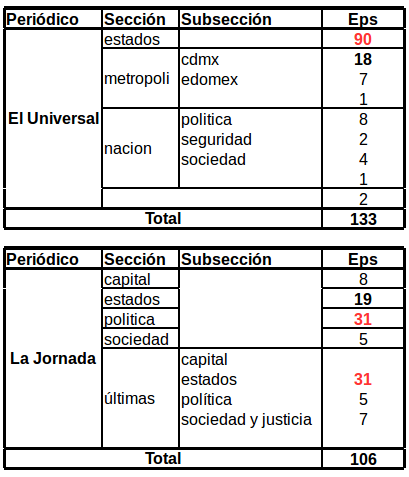
\includegraphics[scale=0.5]{img/2.7_LaJornada_ElUniversal_secciones.png}
\par\bigskip
\small Fuente: Elaboración propia.
\end{minipage}\bigskip





\subsection{El Diario La Jornada}
\label{sec:LaJornadaDiario}

El LAOMS observó, en un análisis preliminar\footnote{
    Comparando exhaustivamente a los diarios \emph{La Jornada}, \emph{El Universal} y \emph{Reforma} en sus versiones impresas; aunque sus resultados nunca fueron publicados, este análisis preliminar se realizó para publicaciones de 2011 y 2012, del cual sólo se tiene respaldo hemerográfico de los artículos publicados.
}, que en términos de frecuencia absoluta, \emph{La Jornada} concentraba una mayor cantidad de reportes sobre protestas que otros diarios comparados\footnote{
    Lo cual es consistente con los resultados hallado en la figura \ref{2.3_sesgoRegional}. 
    No obstante, aunque \emph{El Universal} le supera en cobertura, suponemos que esto se debe a la plataforma de difusión adoptada y la implementación de nuevas mecánicas operativas para el medio. 
    Ya que no existen las limitaciones de espacio de la versión impresa, \emph{El Universal}  ha optado por incrementar el número de sus publicaciones a través de actualizaciones constantes de sus corresponsales.
}, por lo que tomó la decisión de seleccionar a este medio como única fuente de referencia por un criterio cuantitativo y de conveniencia; primero extrayendo contenido de su versión impresa y después de su versión en línea\footnote{Aunque sin considerar la sección de \emph{últimas}, que es exclusiva de su sitio web y fue implementada a partir del 1 octubre de 2013.}.

Se eligió cambiar el soporte debido a que resultaba más fácil extraer contenido, las noticias cuentan con un buen indizado, las búsquedas se simplifican y la mayoría del contenido de la versión impresa (a excepción de una pequeña porción de noticias, usualmente breves) era publicado en la versión en línea de forma idéntica. 
Este cambio fue producido a finales de 2013, por lo que una porción de la base de datos mezcla estos soportes, implicando cierto nivel de pérdida, no mayor a una decena de noticias al mes (según respaldos hemerográficos revisados de enero, abril, junio y julio de 2012).


\emph{La Jornada} ``se ha encontrado entre los medios más importantes de la oposición y tiene la reputación de ser más independiente del gobierno que otros periódicos'' \citep[119]{2003_Wada_Tesis}, por lo que su tendencia periodística (y consecuentemente su sesgo) es particular en el medio. Interpretamos la información extraída de este diario (normalizada por los esquemas de codificación) bajo la perspectiva de la esfera pública
\footnote{A pesar de que el LAOMS (por el momento en que se encuentra el desarrollo de proyectos al interior del laboratorio) opta por una salida \emph{representacional}, que ``da por sentada la parcialidad informativa tratando de mantenerla constante y asumiendo el propósito de relevar propiedades cualitativas de las protestas por encima de su potencial exactitud contable'', sosteniendo la compilación de registros en torno a un solo periódico ---\citep[3]{2017_Urbina_estudiantes}---.} 
---descrita en la sección \ref{sec:esfera_publica}--- donde se corroboran y amplían las características precisadas por \citet{2003_Wada_Tesis}\footnote{Según estas características, en su propio estudio histórico de los movimientos sociales en México, \citet{2003_Wada_Tesis} utiliza a \emph{La Jornada} en comparación con \emph{Excélsior} (identificados por su posicionamiento de ``izquierda'' y de ``derecha'', respectivamente) entre los años 1985--2000.} para la selección de un medio adecuado: \emph{diferencia} (de lectores en términos de su posición política), \emph{importancia} (en el espacio público representado) e \emph{influencia} (hacia élites políticas, económicas o intelectuales).






\subsubsection{Diferencia}
\label{sec:LaJornadaDiario_Diferencia}


Según su propia descripción\footnote{Consultada en \url{http://www.jornada.unam.mx/info/} el 29 de mayo de 2017.}, el diario \emph{La Jornada} fue creado en 1984 por un grupo de periodistas que abandonaron \emph{Unomásuno}, con el apoyo de artistas y ha dado cabida a ``voces ajenas a las corporaciones oficiales, a los grupos económicos y financieros, a la industria del espectáculo, a los designios de los grandes poderes y a la moral social hegemónica que no podía concebir 'malas palabras', y ni siquiera giros coloquiales, en el papel impreso''. 
Se ha reconocido además que ``este periódico es generado por los mismos actores sociales ante el vacío estatal, son los movimientos quienes se apropian de las nuevas herramientas para articularse e intervenir en la esfera pública'' \citep[21]{2011_Tesis_LaJornada}. Respecto a su origen y línea editorial son significativas las lealtades que afirman guardar:

\begin{center}
    \begin{minipage}{0.9\linewidth}
        {\setlength{\parindent}{12pt}\small
	    Debemos lealtad a los artistas, intelectuales, académicos, periodistas, políticos y escritores que participaron en la
	    fundación del diario, así como a los estudiantes, obreros, amas de casa, profesionistas, campesinos, pequeños
	    empresarios, promotores de derechos humanos, comerciantes, poetas y desempleados que decidieron arriesgar lo único
	    que tenían en la bolsa, el equivalente de veinte o treinta dólares de aquel entonces, y convertirse en accionistas de
	    nuestro periódico.  \normalsize \emph{La Jornada} ¿Quiénes somos?.
        }
    \end{minipage}
\end{center}

Según la interpretación que su directora da a la mirada de \emph{La Jornada} ``somos un periódico catalogado de izquierda, que centramos el interés en el desarrollo de nuestras naciones. (...) Nuestra forma de mirar es crítica, muy compasiva con algunos sectores, como los más desfavorecidos''\footnote{Entrevista a Carmen Lira para Página/12, consultada en \\ \url{https://www.pagina12.com.ar/amp/76927-las-redes-no-tienen-ninguna-credibilidad} el 05 de diciembre de 2017.}. 
A rasgos generales y bajo un acercamiento directo con este diario Arce Barceló escribe sobre él:


\begin{center}
    \begin{minipage}{0.9\linewidth}
        {\setlength{\parindent}{12pt}\small
	    (...) el aporte de La Jornada se constituye como herramienta alternativa de opinión, extendiendo su influencia al tiempo que la población la incorpora en su vida cotidiana, hasta convertirse en un medio generador de cambios concretos en las decisiones y conductas de la clase dirigente. 
	    La Jornada dispone de su propio modelo de organización, línea informativa y editorial, su método de recogida y búsqueda de información, su relación con los movimientos sociales. \normalsize \citep[21]{2011_Tesis_LaJornada}.
        }
    \end{minipage}
\end{center}


Las características del diario moldean en su conjunto el perfil de sus lectores, quienes en términos generales ``forman parte de ese sector ilustrado de capas medias y universitarios que se interesan por la situación del país y del resto del mundo'' \citep[474]{2011_Tesis_LaJornada}. 
Por su puesto, dicha representación es sesgada por su propia línea editorial, que favorece algunos discursos e ignora otros.



\subsubsection{Importancia}
\label{sec:LaJornadaDiario_Importancia}

Aunque lejos de ser un periódico de circulación nacional\footnote{Según información extraída del padrón nacional de medios ---\url{http://pnmi.segob.gob.mx/}---, consultado el 29 de mayo de 2017, se distribuía el mayor número de ejemplares ---76,399, correspondiente al 69.30\% del tiraje total--- en la capital del país.}, \emph{La Jornada} es un medio con gran presencia en distintas regiones del país al mantener ediciones locales en Aguascalientes, Baja California, Guerrero, la región maya (Yucatán-Campeche-Quintana Roo), el oriente (Puebla-Tlaxcala), San Luis Potosí, Veracruz y Zacatecas. 
Más allá del tiraje que pueda reportar ---y las sospechas que estas cifras generan--- se ha argumentado que ``su sección política es la más leída entre las secciones sobre ese tema en los cuatro principales periódicos de información general (\emph{La Jornada}, \emph{El Universal}, \emph{Reforma} y \emph{Milenio})''\footnote{Según el Estudio General de
Medios, Ipsos BIMSA. Además ``Según el informe de Bimsa que cita Expansión, entre los diarios de información
general, el mayor número de lectores lo tiene El Universal, con 419 mil 500; en
segundo lugar se encuentra \emph{La Jornada}, con 287 mil 100; en tercer sitio
aparece Reforma, con 276 mil 700'' ---Pérez Espino, J. en \citep[245]{2011_Tesis_LaJornada}---.} \normalsize \citep[34]{2011_Tesis_LaJornada}.


Según \citet{2011_Tesis_LaJornada} uno de los métodos de \emph{La Jornada} para mantener su autonomía de otros medios de comunicación es la utilización de fuentes de información propias. 
En términos proporcionales para un mes de publicaciones\footnote{Del 19 de mayo al 15 de junio de 2008.},  85.18\% corresponden a su redacción, mientras que el 14.81\% procede de otras fuentes (como agencias de noticias). 
Señala además que la circulación del diario ha repuntado en momento coyunturales, cuando se han reportado eventos políticos y sociales trascendentales a su línea editorial, incluídos eventos relacionados a los movimientos sociales\footnote{Por lo que es de esperar que los ciclos de atención mediática resulten gravemente afectados en protestas de gran envergadura o significado para el diario, como consecuencia del importante papel dado a ciertos movimientos sociales.}. 
Respecto a la cobertura que éstos reciben en sus páginas se hacen interesantes anotaciones:

\begin{center}
    \begin{minipage}{0.9\linewidth}
        {\setlength{\parindent}{12pt}\small
	      Pablo González Casanova (...) apunta que La Jornada da cabida a todos los movimientos con un espíritu crítico y plural. Enjuiciando día a día al neoliberalismo neoconservador de quienes pretenden hacer de México un nuevo ``estado libre y asociado de Estados Unidos''. 
	      A lo que añade que La Jornada da entrada en sus páginas a las más distintas expresiones de una izquierda política en grave crisis, aquí y en el mundo. \normalsize \citep[450--451]{2011_Tesis_LaJornada}.
        }
    \end{minipage}
\end{center}


\begin{center}
    \begin{minipage}{0.9\linewidth}
        {\setlength{\parindent}{12pt}\small
	     Hugo Gutiérrez Vega, (...) coordinador de \emph{La Jornada Semanal} y presidente del Consejo de administración (...) al referirse a la labor del diario lo ubicó como un fenómeno singular: ``creado y formado por periodistas, que busca, por una parte, defender los aspectos esenciales del pensamiento crítico, y por la otra, apoyar a los movimientos de liberación y a las más urgentes reivindicaciones populares''. \normalsize \citep[456]{2011_Tesis_LaJornada}.
        }
    \end{minipage}
\end{center}

\begin{center}
    \begin{minipage}{0.9\linewidth}
        {\setlength{\parindent}{12pt}\small
	    El periodista Hermann Bellinghausen afirmaba: ``no sólo es el periódico de la sociedad civil, sino sobre todo el periódico de los movimientos sociales de México, de América Latina e incluso del mundo. Sin ella sería imposible comprender los pasados 25 años (...)''. \normalsize \citep[458]{2011_Tesis_LaJornada}.
        }
    \end{minipage}
\end{center}


\begin{center}
    \begin{minipage}{0.9\linewidth}
        {\setlength{\parindent}{12pt}\small
	    la mayor parte de las marchas que se realizaban por entonces\footnote{Finales de los 80's.} planificaban su recorrido de tal forma que los manifestantes pasaran frente a sus oficinas de Balderas, 68: ``allí se detenían, para agradecernos la cobertura a sus causas o, en ocasiones, para reclamarnos airadamente el que no les hubiéramos concedido el espacio que creían merecer o que no hubiésemos informado de sus movimientos con el enfoque que ellos querían''. ---Entrevista a Carlos Payán \normalsize \citep[378]{2011_Tesis_LaJornada}---.
        }
    \end{minipage}
\end{center}




\subsubsection{Influencia}
\label{sec:LaJornadaDiario_Influencia}

A pesar de que el periódico asegura que no existen compromisos con grupos de poder político o económico, se han reconocido los vínculos que el diario mantiene con líderes de la oposición, como Andrés Manuel López Obrador\footnote{
    Quizás una de las acusaciones más graves que ha recibido el diario es que ``hubo un tiempo en que siendo Andrés Manuel López Obrador, presidente nacional del PRD, casi diario, en las madrugadas revisaba y cerraba las notas del periódico, como interventor, construyendo verdades absolutas para manipular y denostar, editorializando a su favor, lo que era supuesta información. 
    Desde entonces existe una requisa de contenidos y en \emph{La Jornada} NO existe la libertad de expresión, sino la censura y el control'' cita de: \url{http://www.laotraopinion.com.mx/articulo/amlo-manipulaba-personalmente-la-informacion-de-la-jornada-marco-rascon} (consultado el 05 de diciembre de 2017). 
    Por supuesto, en el ambiente periodístico la descalificación visceral es común, de modo que se debe interpretar con cautela la denostación y el enaltecimiento de todo medio.
} y grupos indígenas\footnote{
    Consultado en \url{https://www.sdpnoticias.com/nacional/2017/11/08/carmen-lira-saade-premio-democracia-2017} el 05 de diciembre de 2017.
}. 
De modo que su ámbito de influencia fluye en ambos sentidos: de grupos de izquierda política y movimientos sociales de mayor impacto al diario y viceversa\footnote{
    Al respecto, resultan significativas las declaraciones hechas por López Obrador (y el respaldo ofrecido a la dirección del diario) ante el conflicto laboral de \emph{La Jornada} en junio de 2017, descalificando el llamado a huelga del \emph{Sindicato Independiente de Trabajadores de La Jornada} (Sitrajor) y valorándolo como una forma de debilitar su propio movimiento; asegurando que ``es un diario indispensable para el movimiento social y democrático de México''. 
    Fuentes:  \url{https://politico.mx/minuta-politica/minuta-politica-partidos-politicos/amlo-lamenta-conflicto-laboral-en-la-jornada/}  y \url{http://www.laizquierdadiario.mx/La-huelga-en-La-Jornada-y-el-desbarranque-de-la-intelectualidad-progresista?id_rubrique=1714} ---consultadas el 05 de diciembre de 2017---.
}. 
Aunque con cierta actitud acrítica, se ha descrito que:


\begin{center}
    \begin{minipage}{0.9\linewidth}
        {\setlength{\parindent}{12pt}\small
	    La Jornada es un proyecto plenamente consolidado. 
	    Es, para una amplia franja de la sociedad, un medio de comunicación indispensable. 
	    Es, para las instituciones, un interlocutor reconocido. 
	    Es, como reza en sus principios fundacionales, un medio plural que da cabida a todas las voces y que con frecuencia es el único vehículo abierto a la divulgación de la información vital de los movimientos populares; el único foro para la crítica y el análisis alternativo, el espacio para la denuncia, cuando la mayoría asume el discurso uniforme que se impone desde los poderes. 
	    Es, en suma, un diario necesario en el México de hoy. \normalsize \citep[475--476]{2011_Tesis_LaJornada}.
        }
    \end{minipage}
\end{center}



Son encontradas las opiniones que desata el diario; Noam Chomsky, reconocido lingüista y activista ha mencionado que \emph{La Jornada} es ``tal vez el único periódico realmente independiente en el hemisferio''\footnote{
Entrevista del 6 de octubre de 2009, disponible en \url{https://www.youtube.com/watch?v=-3kAld2YwgU&t=21s}, consultada el 29 de mayo de 2017.}; mientras que otros medios lo acusan de practicar un periodismo militante, poco crítico de los movimientos sociales y fuertemente ligado a grupos de poder entre la oposición. 
Al respecto puede resultar significativo este fragmento de Óscar Camacho\footnote{Cita de Olmos Rodríguez, J. G. (2014). \emph{Los reporteros mexicanos en la guerra zapatista}. Redactum. p. 81.}, donde escribe sobre la cobertura de la guerrilla del EZLN:

\begin{center}
    \begin{minipage}{0.9\linewidth}
        {\setlength{\parindent}{12pt}\small
	    En Chiapas se presentó el caldo de cultivo para que muchos periodistas dijeran: ``aquí está lo que quería, aquí me muevo a mis anchas'', como fue el caso de muchos periodistas de \emph{La Jornada} entre los que yo estuve. Hay que decirlo, el caso de los enviados de \emph{La Jornada} es el más claro, hicimos un periodismo militante de manera irreflexiva, hubo una especie de inercia de empatía con el movimiento zapatista.
        }
    \end{minipage}
\end{center}


Según \citet{2011_Tesis_LaJornada} en un inicio tanto las instituciones públicas como las empresas privadas se negaban a darle publicidad al periódico, pero a finales de la década pasada\footnote{
Más precisamente, \citet{2011_Tesis_LaJornada} analizó la publicidad que publicó el diario del 19 de mayo al 14 de junio de 2008.} ya se anunciaba publicidad de ambos sectores, aunque de forma irregular e insuficiente; donde el 58\% de los anuncios publicados corresponden al ámbito institucional\footnote{
Donde se incluye tanto a la administración y oficinas gubernamentales, como a organizaciones civiles y sociales.} y el 42\% al ámbito comercial\footnote{
La publicidad de \emph{La Jornada de enmedio} (separata sobre ciencia, cultura espectáculos y deporte) fue analizada de forma independiente por \citet{2011_Tesis_LaJornada}, quien observó también una participación irregular, con un 55\% de anuncios promedio solicitados por anunciantes privados y 45\% por actores institucionales.}, resultando como principal sustento de \emph{La Jornada} las ganancias obtenidas por la venta de sus productos. 
Sin embargo, recientemente las ganancias obtenidas por publicidad, provenientes del gobierno federal se han elevado considerablemente\footnote{Algo que ha sucedido en casi todos los medios de comunicación importantes bajo el sexenio de Enrique Peña Nieto, según  el reporte de \citet{2017_FUNDAR_PublicidadOficial}.}. 
Si \citet{2011_Tesis_LaJornada} indicaba que de enero a julio de 2007 los ingresos por publicidad oficial en \emph{La Jornada} era de 5.35 millones de pesos, \citet{2017_FUNDAR_PublicidadOficial} reporta un monto de 89.73 millones para 2015 y de 85.22 millones para todo 2016\footnote{Es interesante también la comparación entre cifras reportadas para diferentes medios entre un sexenio y otro, donde se observan claras diferencias en el gasto por publicidad.}. 
Esto, aunado a un incremento en la representación positiva de figuras gubernamentales en sus páginas ---que según su orientación, no tendría porque apoyar---, ha hecho que los críticos del diario aseguren que ``actualmente, \emph{La Jornada}, es de los diarios más oficialistas que existen''\footnote{
Fuentes: \url{https://www.etcetera.com.mx/archivo/el-oficialismo-de-la-jornada-en-frases-y-numeros/}, \url{https://www.etcetera.com.mx/opinion/la-mutacin-gentica-de-la-jornada/} y \url{https://www.etcetera.com.mx/opinion/por-que-no-es-lo-mismo-el-golpe-excelsior-que-el-litigio-en-la-jornada/}.}, si bien continúa dando apoyo a figuras emblemáticas de la izquierda política nacional.


Antiguos colaboradores del diario también lo han cuestionado, por lo que consideran una visión sesgada de la realidad nacional:



\begin{center}
    \begin{minipage}{0.9\linewidth}
        {\setlength{\parindent}{12pt}\small
	    \emph{La Jornada}. El nombre del diario me suena: es el que fundamos un grupo amplio de diversas izquierdas. Le pusimos un candado contra la reelección en la dirección. Pero la hoy directora, Carmen Lira, con 20 años apoltronada en la dirección, le dio clases a Hugo Chávez sobre cómo cambiar las reglas y brincarse estatutos. Echó fuera a todos los fundadores y convirtió el diario en boletín del CCH Oriente y en \emph{La Voz de Ocosingo}.  \normalsize ---Luis González de Alba, artículo de la revista \emph{nexos} publicado el 1 de Febrero de 2016, disponible en: \url{https://www.nexos.com.mx/?p=27453}---.
        }
    \end{minipage}
\end{center}


\begin{center}
    \begin{minipage}{0.9\linewidth}
        {\setlength{\parindent}{12pt}\small
	    Señora directora: Después de más de 15 años de trabajo ininterrumpido en \emph{La Jornada}, te presento mi renuncia como colaborador semanal del diario.
	    
	    El motivo es la censura contra mi última colaboración, correspondiente al viernes 12 de noviembre, que trataba el tema de la falta de requisito constitucional de residencia de Andrés Manuel López Obrador para ocupar el cargo de jefe de gobierno de la ciudad de México, así­ como el contenido político que, a mi juicio, tuvo el registro del mismo como precandidato del Partido de la Revolución Democrática.
	    
	    La materia del artí­culo es para mí lo de menos (...) No puedo admitir la censura política, pues toda mi vida he luchado contra ella. No puedo avalar tampoco que en \emph{La Jornada} se pueda opinar de los procesos internos de otros partidos, pero se censure un escrito sobre el proceso preelectoral interno del PRD. El periodismo que defiendo es otro.  \normalsize ---\emph{Deja Pablo Gómez La Jornada}, correo ilustrado del 16 de noviembre de 1999, disponible en: \url{http://www.jornada.unam.mx/1999/11/16/correo.html}---.
        }
    \end{minipage}
\end{center}


\begin{center}
    \begin{minipage}{0.9\linewidth}
        {\setlength{\parindent}{12pt}\small
	    Este diario ha sido un medio muy importante para la democratización del país, fue, La Jornada el primer medio en denunciar el fraude electoral perpetrado por Carlos Salinas de Gortari a Cuauhtemoc Cárdenas. Pero algo ha pasado con este diario, desde el ascenso de López Obrador lo han cobijado, y hasta cierto punto no está mal, pero el diario ha perdido su carácter democrático y se ha vuelto un periódico sectario donde no está permitido criticar a AMLO, y donde no se puede disentir de las opiniones de la ``izquierda dura''. La Jornada se ha ensimismado, se ha cerrado en sí misma, y se ha vuelto un diario lejano a lo plural.  \normalsize ---\emph{Marco Rascón y la Jornada, la censura en la izquierda}, disponible en: \url{http://elcerebrohabla.com/2011/08/18/marco-rascon-y-la-jornada-la-censura-en-la-izquierda/}---.
        }
    \end{minipage}
\end{center}





\subsection{Muestreo de noticias}
\label{sec:NotiMuestreo}

El protocolo para la búsqueda y extracción de noticias periodísticas ha sido modificado a lo largo del proyecto sin que exista una discusión sobre sus implicaciones. 
Ya que no se repitió dicho muestreo bajo un criterio único, los sesgos combinados de estos métodos pueden tener cierta repercusión en los datos que se utilizan para este trabajo. 
Específicamente, se han identificado dos periodos cuya extracción de notas periodísticas resulta distintiva dado el muestreo empleado\footnote{
    Los periodos de cambios y las características de los mismos fueron reportados de forma anecdótica, principalmente por una de las personas que realizó el muestreo de las noticias, además fueron confirmados por otros colaboradores del LAOMS; ya que no existe documentación sobre los cambios en la metodología, nos basamos en los respaldos hemerográficos del laboratorio para definir con precisión las fechas de publicación que diferencian la aplicación entre protocolos. 
    Estas fechas aparecen superpuestas debido a que la base de datos fue alimentada a partir de septiembre de 2013 (con información sobre protestas desde julio de ese mismo año), sólo hasta que se consolidó el proyecto (hacia finales de año), se registraron protestas de periodos anteriores. 
}: 

\begin{itemize}
    \setlength\itemsep{0.5em}
    \item \textbf{\emph{Del 01 de julio al 01 de octubre de 2013}} :
    Las notas correspondientes a este periodo fueron extraídas desde la versión impresa del diario\footnote{
	Como se ha indicado en la sección \ref{sec:Sesgo_plataforma}, existen sesgos generales entre un soporte impreso y digital, también se reconoció en la sección \ref{sec:LaJornadaDiario} que existen noticias breves de la versión impresa de \emph{La Jornada} que no son reportadas en la versión digital. 
	Sin embargo, este sesgo particular por el soporte elegido tiene poca representación en los datos que utilizamos posteriormente, debido a que sólo una noticia es exclusiva de la versión impresa, el resto de ellas también pueden ser consultadas también en la versión digital del diario. 
    }, consultada (a partir del 29 de julio) a través del sitio \emph{issuu}\footnote{
	\url{https://issuu.com/lajornadaonline}.
    }, bajo la lectura de textos en los cuales era común hallar un evento de protesta; la conformación de criterios para descartar o centrar la búsqueda en ciertos contenidos fue gradual y basada en búsquedas preliminares\footnote{
	Por ejemplo, se fueron descartando gradualmente las secciones \emph{mundo}, \emph{deportes} y \emph{cultura}. 
	En el resto del diario, la lectura de contenidos se centraba en los encabezados, primeros párrafos de una noticia, fotografías y sumarios.
    }. 
    Ya que dicha revisión comúnmente no era exhaustiva, los textos donde se resalta la protesta como tema principal tienen mayor probabilidad de ser seleccionados. 
    Se permitía la utilización simultánea de búsqueda textual (a través del buscador disponible en ese sitio) junto a la búsqueda por lectura de los contenidos; 
    sin embargo, la utilización de palabras clave (las cuales no habían sido definidas como protocolo de búsqueda) era sólo complementaria. 
        
    
    \item \textbf{\emph{Del 02 de octubre de 2013 al 31 de diciembre de 2016}}, y del \textbf{\emph{17 de octubre de 2012 al 30 de junio de 2013}}: Como consecuencia de las constantes pérdidas de noticias por búsquedas basadas en la lectura de los contenidos, se creó un listado de palabras clave genéricas ---vinculadas a formas comunes de protestas--- como un método de auditoría. 
    Posteriormente, al comprobar la reducción de tiempo que este tipo de búsqueda conllevaba, se estableció como único protocolo. 
    El motor de búsqueda adoptado es Google; la lista de palabras clave fue ajustada en un proceso gradual, donde se realizaron algunas modificaciones al inicio de su implementación, añadiendo sobre todo términos referentes a protestas menos comunes como caravanas y lanzamiento de proyectiles, constituyendo el protocolo final, resumido en la tabla \ref{TerminosBusqueda}\footnote{
	Es decir, en Google se introduce como  búsqueda la siguiente cadena: \emph{``bloqueo OR bloquean OR caravana OR boicot OR campamento OR huelga OR manifestacion OR manifestantes OR manifestaciones OR manifiestan OR manifestaron OR marcha OR marcharon OR mitin OR movilizacion OR movilizan OR movilizaron OR paro OR pararon OR planton OR plantan OR plantaron OR protesta OR protestaron OR hackean OR tomaron OR ``en demanda'' OR motin OR petardos OR piedras site:http://www.jornada.unam.mx/2016/11/11''}, ajustando la fecha del final con formato \emph{aaaa/mm/dd}, según el día en el que se desee buscar.
    }. 
    La selección de los términos que conforma el protocolo de palabras clave obedece a un criterio de ocurrencia en los textos seleccionados. 
    Es decir, una vez que se seleccionaba una noticia relevante para la definición del evento de protesta, eran contabilizados los términos que parecían relevantes; luego, eran agrupados en conteos de un par de días. 
    Al final, los términos que más se repetían entre los textos seleccionados fueron ajustados en un proceso de prueba y error. 
    Antes de su implementación, se comprobó mediante pruebas puntuales que variaciones de estos términos fueran incluidos en la búsqueda, sin necesidad de introducir una segunda consulta\footnote{
	Se verificó, por ejemplo, que el término \emph{marcha} produjera los mismos resultados que \emph{marchas} o \emph{marchó} y si esto no era así, se introducía un nuevo término. 
	Para que la búsqueda fuera eficiente y sólo se realizara una vez, se utilizaron exactamente los 32 términos que establece Google como límite para la definición de un query. 
	Fuente: \url{https://support.google.com/gsa/answer/4411411\#requests} ---consultada el 06 de enero de 2018---.
    }. 
    A pesar de que no se comprobó en términos reales la efectividad de los términos, el protocolo ha resultado práctico en la detección de noticias que incluyen alguno de los términos genéricos referidos. 
    Aunque se discrimina una gran cantidad de noticias por este método, se pueden detectar concordancias inválidas por polisemia\footnote{
	Es decir, cuando la coincidencia con un término no corresponde a un significado asociado a la protesta, por ejemplo: ``toma de \emph{protesta}''.
    }, 
    además de identificar coincidencias por hipervínculos a otras noticias u otros elementos HTML que no corresponden directamente al texto de la noticia referida (lo cual posibilita el hallazgo de noticias que refieren eventos de protesta, pero que no incluyen en su texto ninguno de los términos buscados). La principal desventaja del método es ---como lo indica \citet{2010_Strawn_keywordSearch}--- que los resultados son consistentes con formas comunes de protesta, lo cual induce una homogeneización presumiblemente detectable por las frecuencias de los repertorios de protesta.
\end{itemize}



\begin{table}[!hbt]
\center
\footnotesize
\caption{Términos de búsqueda usados para localizar eventos de protesta}
\label{TerminosBusqueda}
\begin{tabular}{ | l | l | l | l | } 
\hline
bloqueo & bloquean & caravana & boicot\\
\hline
campamento & huelga & manifestacion & manifestantes\\
\hline
manifestaciones & manifiestan & manifestaron & marcha\\
\hline
marcharon & mitin & movilización & movilizan\\
\hline
movilizaron & paro & pararon & planton\\
\hline
plantan & plantaron & protesta & protestaron\\
\hline
hackean & tomaron & ``en demanda'' & motin\\
\hline
petardos & piedras & & \\
\hline
\end{tabular}
\par\bigskip
\caption*{\small Fuente: Elaboración propia, con información del LAOMS \citep[68]{2017_Cadena_ManualLAOMS}}
\end{table}


La aplicación del primer protocolo contempla un periodo bastante acotado, de forma que nuestros datos estarán determinados predominantemente por la extracción de noticias basadas en la utilización de palabras clave. 
Respecto a este último muestreo, son destacables algunos de los criterios que el LAOMS reconoce para la selección de noticias ---según \citet{2017_Cadena_ManualLAOMS}---:

\begin{enumerate}
    \item La búsqueda se centra en la ocurrencia de eventos de protesta; identificables en el texto de notas informativas, reportajes o crónicas, de acuerdo a la definición \ref{EP}, sin importar su destacabilidad. No se considera su tratamiento u otros aspectos de la noticia\footnote{Se excluyen inserciones pagadas, desplegados, artículos de opinión, entrevistas, columnas, ensayos y editoriales de los cuales no sea posible inferir los elementos que constituyen la definición adoptada del evento de protesta.}.
    \item Se recupera el contenido de forma única, sin importar que un texto refiera varios eventos de protesta o sólo se describa información mínima de uno.
    \item Los artículos se buscan y consignan como registros por día; es decir, que si un evento de protesta se extiende (y reporta en la fuente) por varios días, se recuperan al menos tantos artículos como el número de días en que se haya reportado el evento por el diario.
\end{enumerate}

También se debe tener en cuenta que en la práctica no todos los contenidos periodísticos se pueden discriminar por estos criterios, por lo que se pueden ejercer otras consideraciones discrecionales, vinculadas al seleccionador de noticias, especialmente en casos límite donde no resulta clara la coincidencia del contenido con la definición de evento de protesta adoptada\footnote{
    Ya que una misma persona se encargó de la mayor parte del muestreo y dada su experiencia adquirida, creemos que sus consideraciones son (cuando menos) consistentes para casi todo el periodo analizado.
}.





\subsubsection{Comparación entre protocolos}
\label{sec:NotiMuestreo_ComparacionProtocolos}

De la sección \ref{sec:Sesgo_protocolo_busqueda} suponemos que existen pérdidas de información por la aplicación de un tipo de muestreo. 
Para establecer un punto de referencia que nos permita conocer la magnitud de este sesgo en nuestros datos, se emplearon cuatro protocolos de búsquedas para el mes de abril de 2012\footnote{
    Se eligió este mes aprovechando una búsqueda exhaustiva de noticias, realizada por una persona diferente a la que usualmente selecciona contenidos (lo cual implica que los criterios de selección pueden variar).
}. 
Se encontraron 107 noticias únicas por estos métodos combinados\footnote{
    No se incluyeron casos límite, por lo que sólo se toman en cuenta las noticias que cumplen con mayor rigurosidad los criterios de elegibilidad según el LAOMS.
}, 
donde cada uno presenta pérdidas específicas. 
Las frecuencias diarias son comparadas en la figura \ref{2.8_comparacion_muestreo}, donde se observan diferencias en la tendencia de las series de tiempo resultantes para cada método de extracción de contenido. 


\hspace{-1em}\begin{minipage}{\linewidth}
\centering
\captionof{figure}{Comparación de resultados por tipo de búsqueda} \label{2.8_comparacion_muestreo}
\hspace{-1.8em}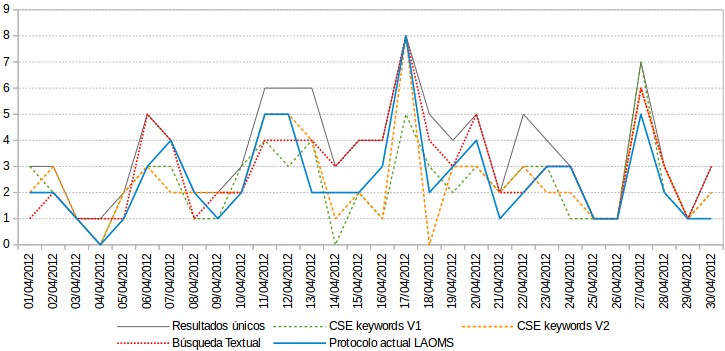
\includegraphics[scale=0.6]{img/2.8_comparacion_muestreo.png}
\par\bigskip
\small Fuente: Elaboración propia.
\end{minipage}\bigskip


De forma general, en seguida describimos las consideraciones asociadas a cada protocolo. 
Es importante observar que más allá de la diferencia en el número de noticias recolectadas, existen singularidades relacionadas al \emph{tipo} de noticias que es posible detectar (u omitir) con cada uno de ellos. 
Se debe tomar en consideración también que aunque algunos muestreos reducen el texto que debe ser revisado, todos dependen en última instancia del criterio personal de quien selecciona las noticias, de modo que la definición del \emph{evento de protesta} debe ser interpretada con particular lucidez:


\begin{description}
    \item[Búsqueda textual] \emph{(88 resultados)}. El método consistió en la lectura de cada una de las noticias del diario en su versión digital\footnote{
	Es decir, todas las noticias que están indizadas en un subdominio de \url{www.jornada.unam.mx/2012/04/}.
    }, 
    a excepción del contenido clasificado en secciones de ``deportes'', ``mundo'' y ``ciencias''. 
    Aunque hasta cierto punto puede ser comparable con el primer protocolo de búsqueda adoptado por el LAOMS, este método tuvo dos ventajas comparadas: la lectura de los contenido fue más exhaustiva y fue complementada con una búsqueda anterior por el mismo método, realizada por una persona diferente\footnote{
	Si bien la proporción de noticias captadas por la anterior búsqueda era muy pequeña para ser significativa.
    }. 
    Es el método que identificó más noticias, pero el que más tiempo consumió (requirió 7 días para una persona dedicada exclusivamente a esta actividad). 
    A pesar de ser considerado un método por ``búsqueda de texto \emph{completo}'', lo cierto es que no se recuperaron algunas noticias, por su carácter estético o como consecuencia de la pérdida de rendimiento de la persona que seleccionó los textos; el número de pérdidas (19 resultados en total) es mostrado en la figura \ref{2.9_perdida_Bcompleta}.
\end{description}
\hspace{-0.1em}\begin{minipage}{\linewidth}
\centering
\captionof{figure}{Pérdida de resultados por protocolo de búsqueda textual} \label{2.9_perdida_Bcompleta}
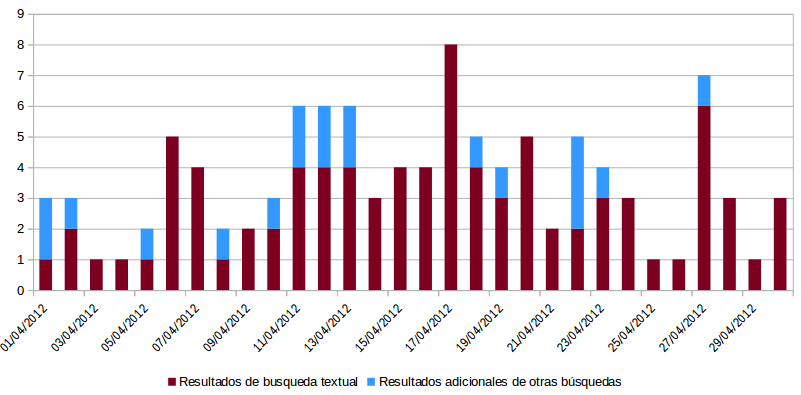
\includegraphics[scale=0.41]{img/2.9_perdida_Bcompleta.png}
\par\bigskip
\small Fuente: Elaboración propia.
\end{minipage}\bigskip
  
\begin{description}
    \item[Protocolo actual LAOMS] \emph{(74 resultados)}. Es comparable hasta cierto punto con el último protocolo adoptado por el LAOMS. 
    Difiere, en primer lugar debido a que el seleccionador de las noticias fue una persona diferente y en segundo lugar, ya que el motor de búsqueda de Google es continuamente actualizado, lo cual afecta la comparabilidad en el tiempo\footnote{
	Algunos cambios del motor de búsqueda son menores, otros tienen mayor trascendencia y pueden llegar a descartar o reordenar resultados basándose en criterios de duplicidad, relevancia, calificación de un sitio, semántica de los términos introducidos o posición geolocalizable desde la que se realiza la búsqueda. 
	Algunos de los cambios confirmados por Google pueden ser consultados en: \url{https://searchengineland.com/8-major-google-algorithm-updates-explained-282627} ---consultado el 06 de enero de 2018---.
	La búsqueda se realizó entre del 15 al 17 de diciembre de 2017 y bajo el conjunto de algoritmos de la versión web ---\url{www.google.com}---, se reordenaron algunos resultados ya mostrados una vez que se cambió de paginación, de modo que se pueden perder resultados si no se examinan con cuidado. 
    }. 
    Aunque se redujeron considerablemente los textos sujetos a revisión, la validación de los resultados requirió de 3 días. En la figura \ref{2.10_perdida_BLAOMS} se representan los niveles de pérdidas diarias (33 resultados en total) que este método generó.
\end{description}
    
\hspace{-0.5em}\begin{minipage}{\linewidth}
\centering
\captionof{figure}{Pérdida de resultados por protocolo de búsqueda LAOMS} \label{2.10_perdida_BLAOMS}
\hspace{-2em}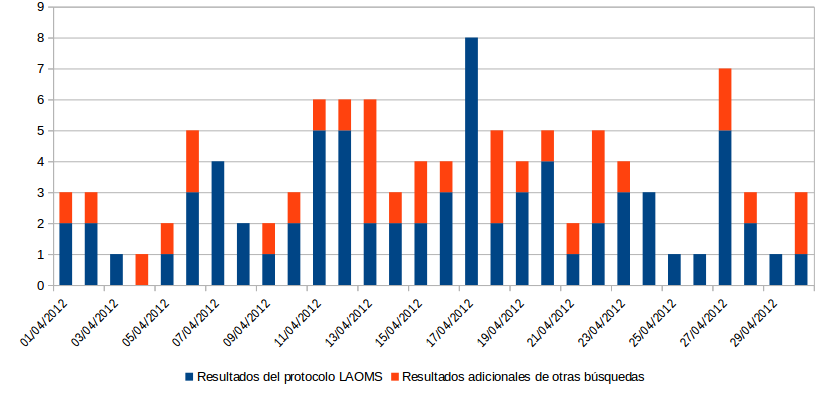
\includegraphics[scale=0.41]{img/2.10_perdida_BLAOMS.png}
\par\bigskip
\small Fuente: Elaboración propia.
\end{minipage}\bigskip

\begin{description}
    \item[Búsqueda por keywords en CSE - versión 1]  \emph{(69 resultados)}. Se utilizaron los mismos términos que en el método anterior, pero cambiando el motor de búsqueda por la API \emph{CSE} de Google para \emph{python}. 
    Aunque es un tema usualmente eludido por Google, se han comprobado la diferencias en los resultados entre la plataforma web y aquellos hallados por su API\footnote{
	Se puede consultar, por ejemplo, esta discusión de un grupo de desarrolladores: \url{https://productforums.google.com/forum/\#!topic/customsearch/8dR2c_MpGho}.
    }. 
    Desarrollamos este método de muestreo recientemente, como una alternativa para reducir aún más los textos que merecen revisión, en él utilizamos \emph{web scraping}\footnote{
	Técnica para extraer contenido (en este caso textos) de un formato HTML.
    } y búsqueda de concordancias para asegurar que las coincidencias se encuentren en el texto de la noticia y tengan una mayor probabilidad de corresponder a un significado vinculado a la protesta. 
    Como restricción adicional, sólo se incluye para revisión el contenido indizado en las secciones ``política'', ``economía'', ``estados'', ``capital'' y ``sociedad''; la revisión de los textos sólo tardó un día. 
    Por ser un método más riguroso se pierden más resultados que en otros protocolos (38 noticias).
    
    
    \item[Búsqueda por keywords en CSE - versión 2]  \emph{(74 resultados)}. 
    Finalmente, ya que se puede iterar entre querys y descartar duplicados a través de \emph{CSE} y \emph{python}, se incrementaron las variaciones de términos y exclusiones desde las consultas enviadas a Google. 
    Tomando como referencia a los textos recuperados por el LAOMS y un nuevo proceso de prueba y error, se definieron estos nuevos querys. Con una pérdida de 33 resultados, las noticias seleccionadas cambian la tendencia reflejada en el protocolo LAOMS (que tuvo una idéntica cantidad de pérdidas) debido a que en este método se discrimina textos de una forma más estricta, aunque se tomen en cuenta mayores variaciones de palabras. 
    Es posible que se pueda mejorar aún más la búsqueda de resultados por la introducción de términos que refieran formas más singulares de protestas.
\end{description}

Aunque las comparaciones que realizamos no son idénticas a la que determinan nuestros datos, ofrecen una pauta de comprobación sobre el tipo de noticias que podemos encontrar en cada periodo donde se cambió el muestreo. 
En el primer protocolo para nuestros datos: ``protestas principales'', de importancia para el diario y que pueden situarse a mayor cercanía respecto a su línea editorial, junto con una porción de noticias halladas por referir formas comunes de protesta. 
Y en el segundo protocolo, esperamos encontrar predominantemente formas comunes de protesta. 
Aunque las variaciones diarias no son mayúsculas, afectan la tendencia de la serie de tiempo y en un acumulado mayor pueden existir pérdidas sistemáticas de noticias relevantes. 



\subsection{Preguntas de investigación}
\label{sec:BaseDDLAOMS}

Los objetivos iniciales del LAOMS propuestos por \citet{2010_Cadena_LAOMS} son ``amplios y ambiciosos'' y consideran tres perspectivas (en resonancia con este trabajo): ``el análisis de organizaciones, el de las redes que forman y los eventos de protesta que desarrollan''. 
Sin embargo, la base de datos que se utiliza para este trabajo tiene un enfoque exclusivo hacia los eventos de protesta, por el que han sido determinadas las preguntas de investigación que tal base pretende contestar\footnote{
Lo cierto es que estas no eran las preguntas iniciales del LAOMS. 
Se han podido identificar 3 fases distintas en las que el proyecto ha evolucionado desde la situación que describe \citet{2010_Cadena_LAOMS}: 
(i) para eventos de protesta reportados entre 2011 y 2012, donde se analizaron noticias de las versiones impresas de \emph{La Jornada}, \emph{El Universal} y \emph{Reforma}, que puede considerarse un periodo de prueba y del cual no existe documentación o bases de datos definitivas 
(ii) que cubre gran parte de los registros originales que se utilizan en este trabajo (específicamente del 01 de noviembre de 2012 al 30 de septiembre de 2015), donde el objetivo era registrar con el mayor detalle posible las protestas reportadas en \emph{La Jornada} durante el sexenio de Enrique Peña Nieto, para lo cual se implementó un esquema de codificación más amplio que el utilizado actualmente; sin embargo, la constante pérdida de información sobre el volumen de participantes, su origen, la resolución de demandas, entre otras características, hizo que se replanteara el esquema de codificación (y por tanto las preguntas de investigación), simplificando las categorías y descartando de antemano los datos que no eran reportados comúnmente por la fuente periodística 
(iii) tras esta reducción se implementó el esquema de codificación actual, que produjo los datos de octubre de 2012 y los de octubre de 2015 en adelante, el cual es una versión reducida (y en algunos casos, modificada) del anterior esquema. Entre éstos dos últimos esquemas, se identificó una equivalencia de campos, de modo que ambas bases de datos fueron unificadas; además, se volvieron a capturar todos los registros que se utilizan en esta tesis, de modo que se asegurara la comparabilidad de la información.}:


\begin{enumerate}
    \item ¿\textbf{Cuándo} ocurren las protestas?
    \item ¿\textbf{Quiénes} protestan?
    \item ¿\textbf{Campo} de los Movimientos Sociales / Acción Colectiva en el que se desarrolla la protesta?
    \item ¿\textbf{Por qué} protestan?
    \item ¿\textbf{A quién} piden que atienda sus demandas?
    \item ¿\textbf{Dónde} protestan?
    \item ¿La protesta es por asuntos (agravios) \textbf{locales}?
    \item ¿\textbf{Qué tan extendida} territorialmente es la protesta?
    \item ¿\textbf{Cómo} protestan?
    \item ¿Qué \textbf{respuestas} tuvo la protesta?
\end{enumerate}

El establecimiento de estas preguntas obedece en primer lugar a los intereses teóricos de la investigación (cuyo fundamento descansa sobre la teoría de la acción colectiva); es decir, que en la práctica sirven ---cuando menos en algunos casos--- como interrogantes retóricas para definir campos vinculados a la definición del \emph{evento de protesta}. 
En segundo lugar, la conformación de las preguntas (y los campos) es consecuencia de la limitada calidad de la información de origen; ya que las fuentes periodísticas no suelen responder a planteamientos más amplios sobre las identidades, características, discursos y acciones de quienes protestan, ni a las causas o consecuencias más generales de las protestas.

Si en el análisis de nuestra fuente de referencia encontramos posibles sesgos de selección, orientados por las prácticas del medio, sus limitaciones y su línea editorial; en este primer punto sobre el que se establece el rumbo de la investigación, se reconoce la normalización bajo la que se conforman los objetivos de la investigación, dirigidos por la información que es comúnmente encontrada en la fuente. 
Esta doble implicación reduce la variedad de la información recolectada, pero también la hace más anticipable y homogénea.

A pesar de todo y de conformidad con la unidad de análisis, éstas preguntas pueden ser algunas de las más sensatas que se han podido establecer de acuerdo a la metodología del AEP, el marco teórico de la investigación y las limitaciones del LAOMS. Ya que las preguntas en sí mismas no son esclarecedoras, para comprender su significado y alcance se debe conocer el esquema de codificación adoptado.



\subsection{Esquema de codificación}
\label{sec:Esquema_codificacion_LAOMS}

Se recuperan algunas anotaciones relevantes sobre los campos que conforman el esquema de codificación actual del LAOMS y sus atributos, cuya numeración entra en correspondencia con las preguntas de investigación planteadas en la sección anterior. 
Un aspecto a tener en cuenta en algunos campos, es la continua inferencia que se realiza a fin de subsanar las limitaciones de la fuente original; a pesar de que cada inferencia tiene una justificación, esto introduce intervenciones no reportadas en los datos finales (pero documentadas en el manual de captura):

\begin{enumerate}
    \item \textbf{Fechas.} 
    De publicación en el periódico y del evento. 
    Si las fechas sobre el evento (cuándo empezó, cubrió o terminó) no son reportadas por la fuente, se hacen algunas inferencias: para la fecha de cobertura se elige el día anterior a la publicación y para protestas que duran varios días, se marca la fecha inicial o final sólo si la noticia a capturar da algún indicio, por impreciso que este sea. 
    Dada la importancia de esta información y ya que se revisaron varias noticias sobre eventos similares, la información de fechas (sobre todo para eventos de protestas de larga duración) fue complementada con información de otras noticias en respaldo\footnote{
    Hubo algunos casos (los menos) donde no se localizó la fecha de inicio o fin de un evento de protesta de larga duración entre las noticias de \emph{La Jornada}, de modo que se tuvo que recurrir a otra fuente periodística. Al ser datos difícilmente tergiversados, se asume que esto no afecta la representación de la protesta para la fuente seleccionada.}.
    

    \item \textbf{Actores.} 
    Se refiere a la información sobre los participantes de la protesta, que pueden ser adscritos a un grupo reconocido (que son el tipo de actores considerados en este trabajo) o sólo ser descritos en la fuente de forma genérica como ``opositores'', ``manifestantes'' o incluso ``vándalos''. 
    Los atributos de cada actor son: \emph{nombre}, \emph{siglas}, \emph{sección} y dos \emph{tipos de actor}. 
    
    El primer problema con este campo es que la fuente difícilmente reporta a todas las organizaciones participantes; puede no indicar su nombre completo y suele omitir sus siglas y sección (ya sea por cuestiones de espacio o debido a que el medio o reportero puede no darles reconocimiento como grupo ---o darles uno diferente al que ellos se adjudican--- por distintos motivos). 
    Esta vez la información referida sobre los manifestantes puede ser tan importante como los detalles omitidos, pues para un medio puede ser más significativo reportar el nombre de una organización reconocida, que dar una precisión detallada cada actor y el tipo de participación que ha tenido en el evento. 
    
    El segundo problema es la inferencia sobre los nombres de los actores cuando estos son descritos de forma ambigua como parte de una organización; de este modo ``sindicato de mineros'' se debe entender como ``Sindicato Nacional de Trabajadores Mineros, Metalúrgicos, Siderúrgicos y Similares de la República Mexicana'', lo que puede inducir a errores de consignación para grupos no conocidos por el capturista o referidos de forma errónea por la fuente\footnote{
    Como criterio adoptado del LAOMS, se puede buscar el nombre correcto de la organización en una fuente externa. 
    Sin embargo, esta fuente externa no es respaldada, ni referida después; además, ya que no todas las organizaciones mantienen un sitio en Internet, esta información puede ser equívoca o referida por terceros.}. 
    
    El tercer problema con este campo es la clasificación teórica de los actores antes de realizar un análisis formal de los mismos; se puede categorizar a los actores participantes como \emph{Organizaciones de los Movimientos Sociales}\footnote{
    Sobre registros cuyos actores fueron clasificados de esta forma se basa este trabajo. 
    No obstante nosotros evitamos su uso (y recurrimos en su lugar a \emph{actores colectivos}, que es un término más genérico), debido a que no todos los actores que fueron categorizados de tal modo se ajustan adecuadamente a la definición sociológica del término.} o actores de otra categoría, pero ya que se requiere de un conocimiento adecuado tanto de la organización, como de los fundamentos teóricos que definen al término ---ver \nameref{AnexoI}---, en la práctica esta distinción puede ser errónea y ha servido en mayor medida para separar actores más o menos reconocidos u organizados de otros\footnote{
    En el manual de captura se indica que la clasificación de actores ---como \emph{Organizaciones de los Movimientos Sociales} (OMS) u otros--- y asignación del campo de interacción ---\emph{Campo de los Movimientos Sociales} (CMS) u otros--- ``depende de dos factores: el ``perfil'' o la especificidad de quienes protestan (...) y las demandas que promuevan o puedan asociarse con otros campos de interacción''. 
    Refiere además que ``si está el nombre de una organización relativamente formal y estable en la noticia y desde el encabezado de la nota o las entradillas se distingue una demanda vinculada al CMS rápidamente se puede determinar que el tipo de acción colectiva de ese EP se trata de una OMS'' \citep[17]{2017_Cadena_ManualLAOMS}.}. 
    
    Un último problema es la consignación de los \emph{tipos de actor}, que pueden ser elegidos en función de una interpretación errónea; el primer tipo según \citet{2017_Cadena_ManualLAOMS}\footnote{
    Aunque esta precisión se realiza para una categoría diferente al de ``Organización de los Movimientos Sociales'', es el indicio más claro que se tiene sobre la asignación de los tipos de actor.} se da en función de una \emph{identidad} que es un concepto ambiguo y requiere conocimiento de la organización; el segundo tipo es consignado a partir de la \emph{demanda} que se presenta en una protesta, que es contextual y en muchos casos imprecisa.


    \item \textbf{Campos de los Movimientos Sociales.} Este es el tipo de dato más teórico de todos y que más juicio requiere por parte del capturista, los campos son sugeridos en su definición ---ver \nameref{AnexoI}--- como ``conjuntos difusos'' y corresponden a interpretaciones sociológicas aún discutidas.
    En su uso regular, se asigna uno o varios campos principalmente en función de los participantes y de las demandas presentadas\footnote{
    Al respecto, el manual de captura sugiere consultar primero los catálogos para campos de acción (CMS u otros): ``para escoger qué campos de interacción son compatibles con el contenido de la demanda, de esta manera se puede determinar el tipo de acción colectiva para ese evento de protesta. 
    Hay ocasiones en las que primero se indica el tipo de acción colectiva y posteriormente el campo de interacción, pero eso también depende de cómo se haya redactado la noticia y de si los sujetos de la protesta son claramente identificables'' \citep[17]{2017_Cadena_ManualLAOMS}.} y secundariamente por las suposiciones del capturista sobre lo que los campos debería medir, por lo que ---hasta cierto punto--- es un campo derivado, pero cuyas interpretaciones tienen gran relevancia teórica en el proyecto. 
    
    Al analizar nuestros datos, se intentó crear una función indicatriz que estableciera una relación directa y formal entre cada tipo de actor y demanda a un CMS; ya sea por medio de categorizaciones binarias o por asignaciones en conjuntos difusos, sin embargo, las funciones deducidas resultaron deficientes dada la inconsistencia de categorías y el pobre diseño relacional entre ellas. 
    
    A pesar de que no utilizamos este dato, sigue siendo relevante, ya que si en el proceso de captura se consideró que las demandas de un actor no se ajustaban en absoluto a ningún campo del \nameref{Anexo_CMS}, los actores no se clasificaron como \emph{Organizaciones de los Movimientos Sociales} ---por lo que el subconjunto de datos que se utiliza en este trabajo depende de la selección de uno o más CMS---.
    

    \item \textbf{Demandas.} 
    La intencionalidad de este campo es registrar las demandas asociadas a cada protesta, guardando cierta fidelidad con lo reportado originalmente por la fuente. 
    Sin embargo, ésta no siempre reporta alguna \emph{demanda textual}, expresada directamente por los manifestantes; sino que en su lugar puede registrar \emph{peticiones}, \emph{exigencias}, \emph{reivindicaciones}, \emph{pretensiones} u \emph{objetivos} (a menudo agrupados y ocasionalmente confundidos) expresados en la manifestación\footnote{
	Como resultado, se pueden encontrar como \emph{demandas textuales} frases genéricas, que deben ser tomadas con cautela (toda vez que pueden no referir situaciones equivalentes), como: ``instalar mesas de negociación'', ``en contra de la reforma educativa'' o ``alto a la violencia''. 
    }. 
    De modo que esta información textual, su paráfrasis y ocasionalmente otras ampliaciones relevantes (con información adicional hallada en la noticia, que aclare su contexto) son recuperadas\footnote{
	A pesar de ello, durante nuestra depuración, se ha realizado una pequeña agrupación sobre ``demandas textuales'' que incluyeron mínimas variaciones debido al fraseo heterogéneo de una misma demanda.
    } y clasificadas en dos niveles. 
    
    Las clasificaciones y subclasificaciones creadas por el LAOMS han sido derivadas de los textos, por lo que reflejan lo publicado en el diario. 
    Sin embargo, no todas ellas tienen la misma relevancia en los datos que analizamos en este trabajo, por lo que (tomando a las subclasificaciones de su esquema de captura como referencia) se agruparon demandas con una pequeña representación o cuya temática resultaba análoga, conformando el \nameref{Anexo_ClasificacionDemandas}. 
    
    Una limitación del registro de demandas ---promovida desde la fuente---, es que estas son asociadas al evento, no al actor que las presenta. 
    Además, las categorías empleadas no consideran (lo cual es inevitable) toda la variedad de demandas reportadas; algunas de ellas (las más comunes) se ajustan perfectamente a los catálogos, mientras que otras más inusuales deben ser forzadas a entrar en una clasificación. 
    Al respecto, consideramos que ``las demandas son narrativas sin límites auténticos'' \citep[186]{2003_Wada_Tesis}, de modo que existe una frontera difusa entre ellas; si bien, un análisis cualitativo minucioso puede aventajar nuestro recuento simple, creemos que las categorías creadas suponen una aproximación válida desde una perspectiva panorámica. 

    
    Por último, a pesar de que nuestros datos tienen una acotación temporal que difícilmente registra ``cambios históricos''\footnote{
	Argumentación central de \citet{2003_Wada_Tesis} para justificar un \emph{análisis de demandas}, dado que diversos investigadores han considerado que las demandas reportadas por los diarios no son fidedignas, ya que son sesgadas por las impresiones de los reporteros. 
    } 
    encontramos que la justificación sobre ``filtrar demandas significativas ante una multiplicidad de discursos'' \citep[168]{2003_Wada_Tesis} es válida, considerando además que las clasificaciones establecidas funcionan adecuadamente como descripciones, enfatizadas dentro de la esfera pública. 
    
    
    
    \item \textbf{Ante quién se protesta.} Se registra ante quienes se manifiestan los actores, clasificando a dichos grupos por ámbito (público, privado o social), función (nivel organizativo) y organismo individual (institución, empresa o agrupación). 
    Se puede inferir ante quién se protesta ---si la fuente no lo indica--- por el lugar elegido para protestar (por ejemplo, los pinos por su asociación con el ejecutivo federal). La mención de los grupos ante los cuales se protesta puede ser explícita, implícita o incidental.
    

    \item \textbf{Lugar de la protesta.} Estado, municipio y lugar (o lugares) reportado por la fuente. 
    Si a partir de la información de la fuente sólo se indica el lugar o municipio, se llenan niveles geográficos superiores buscando información sobre la ubicación. 
    Aún cuando la fuente reporte únicamente la ocurrencia de una protesta en un estado del país (sin precisar el municipio) se considera una referencia válida a un evento. Ocasionalmente las noticias sobre protestas asocian la presencia de un mismo actor en diferentes sitios con idénticas demandas, en tales casos se realiza una agrupación por municipio. 
    

    \item \textbf{Lugar de agravio.} Indica si el motivo por el que se protesta surgió en el mismo estado en que se manifestaron los actores o refiere a agravios de otro estado, nacionales o internacionales. 
    Raramente esta información es explícita en una noticia, por lo que se suele inferir ---si no se hace dicha precisión--- que la protesta surge de un agravio local; lo cual no es necesariamente cierto.
    

    \item \textbf{Alcance territorial.} Local, regional o nacional. Será local ---de nuevo, basándose sólo en inferencias sobre lo publicado por el medio--- a menos que la fuente reporte múltiples eventos de protesta, llevados a cabo en la misma fecha, por un mismo actor y con idénticas demandas en diferentes estados; lo cual es poco común y requiere de la comparación de todas las noticias en un día recuperadas en el proceso de muestreo. 
    Para que este campo tuviera una alta validez, el mismo diario tendría que hacer una conexión entre eventos; ya que los actores participantes pueden ser referidos como organizaciones independientes (y por lo tanto sus protestas serían consideradas como eventos de alcance local\footnote{
	Prácticamente ningún actor tiene auténtica presencia nacional. 
	Aún los actores que tienen gran presencia en el país son a menudo fragmentados bajo liderazgos locales o regionales; por otra parte, grupos locales sin aparente conexión pueden estar relacionados por redes de participación nacional, lo cual posibilita eventos de protesta coordinados de gran alcance.
    }). 
    Por otro lado, aún si la fuente establece esta conexión, la base de datos no relaciona eventos de protesta entre sí.
    

    \item \textbf{Repertorio de protesta.} Actividades que desarrollan los actores colectivos para protestar ---ver \nameref{Anexo_RepertoriosPacificos} y \nameref{Anexo_RepertoriosPacificos}---. 
    Su dicotomía, que clasifica una actividad como \emph{pacífica} o \emph{violenta} es establecida por el énfasis u omisión que una noticia hace sobre agresiones por parte de los manifestantes, ya sea por iniciativa propia o como respuesta a una agresión de otro grupo. 
    Donde su objetividad es particularmente incierta en tomas de casetas e instalaciones, retención de vehículos y protestas sin descripciones específicas, que se consideran actos pacíficos a menos que la fuente especifique violencia en su ejecución.
    

    \item \textbf{Respuesta de la protesta.} Su propósito es registrar, según lo dicho por la fuente, ``si hubo interlocución con los demandados, si las demandas se atendieron parcialmente o por completo, si se utilizó la fuerza pública y si la misma fue brutal o proporcional'' \citep[34]{2017_Cadena_ManualLAOMS}. Esta respuesta debe ocurrir durante el evento o poco después del mismo, ya que de otra forma difícilmente será cubierta por una fuente periodística.

\end{enumerate}

Cabe mencionar que los criterios aquí mencionados se consideran de mayor relevancia, pero una descripción más precisa sobre el proceso de captura puede ser consultada en \citet{2017_Cadena_ManualLAOMS}.



\subsection{Proceso de captura}
\label{sec:captura}

Recientemente, el LAOMS ha centrado su atención en la captura de información, la cual es continuamente discutida para asegurar cierta homogeneidad; su manual de captura es actualizado constantemente para proporcionar una mejor interpretación de los campos; 
y la organización de las tareas de codificación incluye el registro y seguimiento de asignaciones de forma puntual y eficiente. 
Adicionalmente, se ha implementado una plataforma web\footnote{
    A través de la aplicación de código abierto \emph{LimeSurvey} ---ver \url{https://www.limesurvey.org/}---, que permite el desarrollo, publicación y recolección de resultados de encuestas en línea con un mínimo de conocimientos en programación.
    Gran parte de los registros de nuestra base de datos fueron capturados en otro sitio de desarrollo propio, pero han sido revisados en la plataforma de \emph{LimeSurvey}. 
} 
(cuya captura parcial presentamos en la figura \ref{2.11_plataformaLAOMS}) que posibilita la captura remota de la información, haciéndola más eficiente y reduciendo la probabilidad de fallos no intencionales en el llenado de los atributos. 



\hspace{-1.5em}\begin{minipage}{\linewidth}
\centering
\captionof{figure}{Plataforma web para la captura de eventos de protesta.} \label{2.11_plataformaLAOMS}
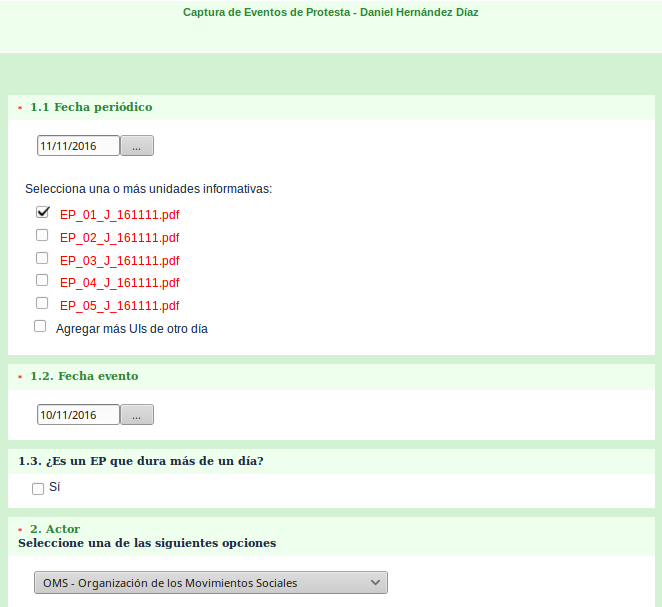
\includegraphics[scale=0.68]{img/2.11_plataformaLAOMS.png}
\par\bigskip
\small Fuente: Laboratorio de Análisis  de Organizaciones y Movimientos Sociales (LAOMS).
\end{minipage}\bigskip


De orden técnico, existe una restricción adicional relevante en la base de datos del LAOMS. 
Ya que su estructura es la de una tabla simple no relacional (dentro del manejador de base de datos \emph{MySQL}) tiene un número limitado de atributos, por lo que no se pueden registrar más de un número determinado ---aquí indicado entre paréntesis-- de: actores (18), demandas (8) y objetivos (3). 
Es raro (pero no imposible) que esta característica límite los datos finales recabados; en los 583 registros datos que utilizamos en este trabajo se alcanzó el límite de demandas 2 veces y el de objetivos 22 veces. La repetición de atributos idénticos (la base original se compone de 506  atributos) aumenta el tamaño en bytes de la base y hace necesario cierto procesamiento para hacer descripciones simples sobre este tipo de información. 
No es un diseño recomendable, pero resulta preferible para el LAOMS, ya que su opción resulta más barata, flexible y fácil de implementar que un desarrollo propio; lo cual refiere a una perspectiva peculiar sobre desarrollos informáticos, oscurecidos por una colaboración poco común con las ciencias sociales en México. 
Al respecto, describen conflictos con una plataforma anterior\footnote{
    Denominada \emph{Telemática para la Investigación y la Docencia Interdisciplinarias} (TIDI), desarrollada en php como una implementación ad hoc. 
    Sin embargo, esta herramienta era aún peor ---debido a la falta de comunicación multidisciplinaria e improvisación metodológica reinante al inicio del proyecto---; donde los registros eran redundantes, tenían problemas de actualización y su integridad estaba comprometida. 
    La TIDI fue utilizada para capturar eventos de protesta en la base LAOMS, ocurridos entre el 31 de Octubre de 2012 y el 29 de Septiembre de 2015; si bien se migró tales datos a la implementación actual en \emph{LimeSurvey}, ésta plataforma anterior no tenía restricciones suficientes para evitar errores de consignación, lo cual podría promover omisiones en la selección de la submuestra (ver sección \ref{sec:submuestra}). 
}, 
utilizada en la mayor parte del proyecto y desarrollada también para el registro de las protestas y sus características: 




\begin{center}
    \begin{minipage}{0.9\linewidth}
        {\setlength{\parindent}{12pt}\small
        (...)
        El desarrollo de soluciones ad hoc toma tiempo; es más costosa que la compra de una licencia de cualquier software común; su desarrollo requiere de conocimientos muy especializados y bien cotizados en el mercado de trabajo, lo que dificulta encontrar colaboradores dispuestos a ganar lo que pagan las universidades públicas. 
        En fin, no es tan sencillo como poner etiquetas a campos en una hoja de Excel o Access. Como todavía son contadas las personas que se encuentran en esta interface de diálogo y colaboración entre ciencias sociales y tecnología es muy fácil generar dependencia hacia esas pocas personas ---diríamos que ocupan una posición central en la red del conocimiento con todas las consecuencias del caso--. 
        Si esa persona se va, o se sobrecarga de trabajo, es muy difícil reemplazarla, todas las actividades se retrasan, lo que obliga a regresar al uso de métodos más accesibles de comunicación y de manejo de la información, sobre los que el equipo de investigación tiene más control y opciones de reemplazo. 
        Otro problema es que el desarrollo de aplicaciones, el software, se convierte en prácticamente un monopolio, porque sólo el desarrollador lo conoce y lo puede modificar, lo cual acentúa esa tendencia a convertir a los especialistas en figuras clave del proceso. 
        (...) Quizá esta situación sea temporal y cada vez sea más sencillo encontrar especialistas dispuestos a desarrollar aplicaciones tecnológicas para la investigación  en ciencias sociales que acepten trabajar con recursos escasos, que tengan tiempo y la paciencia necesaria para comunicarse con personas que aunque hablen español, lo hacen en otro lenguaje especializado \normalsize  \citep[237--238]{2015_Cadena_Tecnologia}.
        }
    \end{minipage}
\end{center}



\subsection{Submuestra seleccionada para este trabajo}
\label{sec:submuestra}

Los datos que se usan en este trabajo son considerados una submuestra de la base datos del LAOMS, centrada en protestas colaborativas entre actores reconocidos (alrededor de movimientos sociales típicos). 
El periodo elegido para seleccionar eventos de protesta (del 17 de octubre del 2012 al 31 de diciembre de 2016) ha sido establecido por conveniencia, ya que sólo se tenía acceso a esta información al momento de realizar nuestra extracción. 

Ya que no es posible evaluar la confiabilidad de esta información, consignada por los primeros capturistas, sin rehacer gran parte del trabajo original y debido a que las categorías del esquema de codificación y los criterios para su llenado son altamente volátiles e inconsistentes a lo largo del periodo considerado, no se presentan índices de confiabilidad entre capturistas ---como lo recomienda una buena práctica del análisis de contenido---. 
Sin embargo, antes de hacer la selección de datos para este trabajo, el equipo del LAOMS realizó correcciones a registros con información faltante, inconsistente o contradictoria (547 registros en total) por lo que se minimizó su impacto ---aún así, este es desconocido---. 

Ante los cambios en el esquema de codificación, se optó por corregir todos los registros utilizados, lo cual favorece a una normalización de la información; realizada sólo por el autor de este trabajo, esto incluye dejar decisiones de captura en manos de quien además realizará el análisis. 
No obstante, algunos sesgos de captura originales podrían perdurar; ya que el subconjunto de datos seleccionado para este trabajo fue extraído con base en registros previos, que consignaron la coparticipación de dos o más actores ---clasificados como \emph{Organizaciones de los Movimientos Sociales}--- en un mismo evento de protesta.

Como referencia, se puede dimensionar que la base de datos del LAOMS mantiene para el periodo considerado aproximadamente\footnote{
    Las cifras que se presentan son consideradas aproximaciones, debido a que se necesitan depuraciones adicionales para poder contar con precisión  y bajo un sólo criterio el número de eventos de protesta para un periodo dado; más allá de contar protestas, varios campos han tenido múltiples cambios en toda la base de datos. 
    Es también debido a esta inconsistencia entre criterios que no se reporta o utiliza en el análisis más que una fracción de los datos de la base ---aquellos que han sido depurados exhaustivamente---, aún cuando hay disponible una gran cantidad adicional de datos.
} 
9,685 registros de eventos de protesta; filtrando los eventos cuyos actores fueron clasificados como \emph{Organizaciones de los Movimientos Sociales}, se detectan aproximadamente 4,034 registros; luego de añadir un tercer filtro, seleccionando los eventos que contaban con la coparticipación de dos o más actores, se obtuvieron 693 registros; únicamente éstos últimos fueron corregidos de forma exhaustiva, de modo que se obtuvieron finalmente sólo 583 registros válidos, los cuales son utilizados en este trabajo\footnote{
    Como comparación, \citet{2012_Wand_andSoule_ColabiracionOMS} mencionan que sólo el 9\% de los eventos capturados en la base \emph{The Dynamics of Collective Action} (que cubre protestas estadounidenses de 1960 a 1995) registran la participación de más de una organización (cuyo único requisito es su mención periodística en una protesta). 
    En nuestro caso, este mismo porcentaje (considerando la aproximación de registros totales) es de 6\%.
}. 
Sobre la diferencia entre estas últimas dos cantidades: 73 registros fueron descartados por incompatibilidad en criterios de agrupación, 63 registros fueron descartados por errores de captura, registros duplicados o información imprecisa durante la consignación del tipo de actor, fechas o número de actores; la diferencia restante (de 26 eventos) fue debido a que no se habían capturado algunos eventos o registros incompletos cumplieron los criterios de selección luego de la depuración del LAOMS.




\subsection{Datos covariables de actores colectivos}
\label{sec:DatosOMS}

Un problema adicional sobre los actores colectivos recuperados de la base de datos del LAOMS es que en su listado se mezclan organizaciones de todo tipo; desde grupos semi-clandestinos de corta duración en los que participan sólo un puñado de personas, hasta agrupaciones nacionales de larga trayectoria y constituidas por miles de agremiados. 
Ya que este trabajo analiza las relaciones entre estos grupos por su asociación en protestas, conocer (así sea de forma superficial) aspectos organizativos de dichos actores colectivos resulta de vital importancia para comprobar si tales atributos influyen en las estructuras sociales deducidas.

Sin embargo, el análisis de los \emph{actores colectivos} implica una ardua tarea. De forma similar a los \emph{eventos de protesta}, su definición y el registro de sus características no obedece a criterios de común acuerdo, sino más bien a interpretaciones difusas sobre algunos de sus atributos que resultan relevantes para ciertos criterios de investigación que acotan su diversidad y complejidad. Considerando solamente a organizaciones civiles en México, se pueden considerar de forma amplia que:


\begin{center}
    \begin{minipage}{0.9\linewidth}
        {\setlength{\parindent}{12pt}\small
	    (...) son formas estructuradas de la acción social, organismos que emanan de la sociedad civil y en consecuencia se definen a partir de su autonomía con relación al gobierno; su principal objetivo no es el lucro aunque bien puedan estar creando productos para el mercado; no son iglesias pero ello no excluye su posible origen religioso o inclusive su indiscutible vínculo con alguna iglesia; del mismo modo no son partidos políticos, por cuanto no se trata de estructuras organizadas cuyo fin principal es obtener o alcanzar el poder político, esto es, la dirección de la nación, aunque muchas de ellas estén motivadas por lograr un proyecto de nación alternativo. Las OCs nunca son neutrales por cuanto, tácita o implícitamente, mantienen ciertos objetivos políticos. Lo distintivo, en todo caso, es que centran su actividad política en dos sentidos, primero, como instrumentos que buscan y logran la participación ciudadana y segundo, por cuanto se convierten en intermediarios entre la ciudadanía y el poder político, sirviendo como vigías del buen funcionamiento de los partidos y el gobierno.  \normalsize \citep[75--76]{2015_Calvillo_DimensionesOC}.
        }
    \end{minipage}
\end{center}


Alternativamente, podríamos referirnos a \emph{asociaciones} de forma aún más general como:


\begin{center}
    \begin{minipage}{0.9\linewidth}
        {\setlength{\parindent}{12pt}\small
	     (...) agrupaciones que se caracterizan por tener a) una membresía predominantemente voluntaria y más o menos formalizada; b) reglas aceptadas de funcionamiento; y c) el acuerdo de los asociados en los fines que persiguen, lo cual delimita su acción y les proporciona cohesión e identidad.  \normalsize \citep[85]{2012_REDA_EvaluacionAsociaciones}.
        }
    \end{minipage}
\end{center}

El segmento que originalmente el LAOMS pretendía recabar es el de organizaciones más o menos estables\footnote{
    Nombradas \emph{Organizaciones de los Movimientos Sociales}, al menos para la porción de datos que se usan en esta tesis ---ver \nameref{AnexoI}---.
}, que en su conjunto representan al sector permanentemente organizado de los movimientos sociales (el cual incluye, por ejemplo, sindicatos, grupos gremiales y organizaciones civiles).  
En la práctica, los datos recabados consideran también actores de existencia breve, cuya participación en protestas solamente es documentada una vez\footnote{
    Si bien se ha advertido que los datos indican ``que las OMS que mantienen actividades regulares son la excepción más que la regla'' \citep[13]{2016_Cadena_OMS}.
} 
o de los cuales casi no se ha podido obtener información fidedigna más allá de la que reporta \emph{La Jornada}. 
Otro problema es que aún organizaciones que son fácilmente vinculables con un movimiento social, pueden encontrarse fragmentadas (organizativa e ideológicamente); si \citet{2016_Cadena_OMS} nos previene sobre una interpretación fácil de unidad al referir un movimiento social, se puede articular un argumento análogo para la aparente unidad de las organizaciones recabadas, dependiendo del nivel al que se lleve el análisis. 
Aunque el estudio de los actores nos conduzca a categorizaciones más o menos cerradas que faciliten el estudio de sus relaciones\footnote{
    Así sean derivadas exclusivamente de su representación en protestas.
}, no debemos olvidar que estos grupos son organismos vivos y complejos que responden de diferente forma a estímulos, con tasas de aparición y desaparición altas ---\citet{2015_Calvillo_DimensionesOC}---, entre las cuales se pueden encontrar ejemplos heterogéneos que nos conduzcan a suposiciones igualmente distintivas. 


Por otro lado, no existe ningún catálogo que registre a todos los grupos sociales considerados; a pesar de que existe un \emph{Registro Federal de las Organizaciones de la Sociedad Civil} (RFOSC)\footnote{
    Consultable en \url{http://166.78.45.36/portal/}.
} y que \citet{2015_Calvillo_DimensionesOC} refiere al \emph{Sistema de Información sobre Organizaciones Sociales} (SIOS) del \emph{Instituto Nacional de Desarrollo Social} (INDESOL) y al \emph{Centro de Documentación e Información sobre OCs} (CEDIOC) de la UAM-I, algunos de estos centro han desaparecido y sus esfuerzos sólo consideran una porción mínima de los actores colectivos en protestas registradas, los cuales (dado su carácter volátil) hacen caduco casi cualquier listado al poco tiempo de su publicación ---si bien su análisis resulta relevante para entender las dimensiones cuantitativas de estos actores sociales---.


\citet{2012_REDA_EvaluacionAsociaciones} crean un protocolo para la evaluación de asociaciones que considera la complejidad ---cuyo grado remite a sus propiedades constitutivas--- como principio de clasificación, de forma ``que no se apliquen estándares similares de desempeño a organizaciones que en realidad resultan muy diferentes'' (pag. 85). 
Diseñan además una \emph{ficha de asociación} (cuyos fines son documentales y analíticos, más que de evaluación) por medio de la cual se pueda tener una imagen más completa de un actor. 
Sin embargo, tal ficha considera una buena cantidad de información que no es fácilmente accesible y que puede resultar inconsistente si no se tiene contacto directo con miembros de la organización, lo cual resulta demasiado costoso\footnote{Sobre todo considerando que el autor de estas líneas ha sido la única persona dedicada a obtener y comparar la información sobre los actores.}. 
El mismo protocolo sugiere a la Internet como una de las fuente de información pertinentes para el llenado de la ficha de asociación; pero se debe considerar que esta fuente es poco confiable e inestable, de modo que los fallos de consignación pueden ser comunes (por interpretación de conceptos, ante información imprecisa o porque la fuente no reporta ciertas características sobre las organizaciones). 

Aunque se han tomado como referencia los doce primeros puntos de la ficha de asociación antes referida para obtener información sobre los actores, se han simplificado los campos; cuyo llenado es derivado de información hallada en sus redes sociales, páginas oficiales o personales de miembros relevantes, sitios de organizaciones afines que les describen u otras noticias periodísticas. 
Nuestras fuentes han sido consultadas de septiembre a octubre de 2017. 
Reconocemos que este no es un método ideal de recolección de información, los datos que se han obtenido no implican más que una visión superficial y desproporcional de representación pública en la red; sin embargo, se considera un modesto punto de partida, desde el cual quizás sea posible mejorar la comprensión de los actores y sus relaciones en protestas. 
Los atributos recabados en este esquema, asociables a cada actor colectivo, son: 

\begin{description}
    
    \item[Sector.] Se refiere a los dos ``tipos de actor'' considerados en el esquema de codificación del LAOMS. 
    Debido a los problemas de imputación referidos anteriormente, se determinaron ambos de acuerdo al \nameref{Anexo_TiposDeActor}, pero tomando como criterio la filiación de los objetivos principales (descritos por nuestra fuente) con un \emph{tipo} particular. 
    De esta forma, siempre que fue posible asociar los objetivos propuestos con un tipo de actor, se llenó sólo el \emph{tipo uno}, que puede considerarse primario; por otra parte, el \emph{tipo dos} es llenado si el anterior tipo no caracteriza por completo los objetivos principales de un actor y puede considerarse secundario. 
    Bajo esta perspectiva, es cualitativamente diferente una organización cuyo tipo uno es \emph{Sindicato de trabajadores del sector público} (SPB) y tipo dos es \emph{Educadores} (ED), de otra cuyos \emph{tipos} son invertidos (ES/SPB); en el primer caso, suponemos que tal actor tiene como principal propósito la defensa de sus agremiados desde el punto de vista del sindicalismo educativo y en el segundo, si bien sus participantes forman parte activa de un sindicato, se organizan al margen de este o incluso como una oposición a él, conformada por educadores cuyos objetivos son propios de su gremio. 
    Ya que nuestras fuentes no siempre declaran explícitamente estos objetivos, se considera el \emph{tipo de actividades} que un actor realiza como criterio secundario, el cual es posible conocer a través de medios periodísticos u otra información indirecta. 
    Aunque la mayoría de los \emph{sectores} pueden ser caracterizados por estos dos criterios, existen casos (principalmente de grupos informales) en que esto no es así; por lo que se recurre a una \emph{descripción del actor} por parte de terceros como criterio adicional.
    
    
    \item[Tipo de organización.] Según \citet{2017_Cadena_ManualLAOMS}\footnote{
	Aún cuando esta distinción organizativa es realizada desde el manual de captura del LAOMS para distinguir a las \emph{Organizaciones de los Movimientos Sociales} entre sí, en la práctica no se utiliza. 
	Pese a que no nos referimos a tales OMS, consideramos que esta categorización es adecuada para los \emph{actores colectivos} que se sugieren en este trabajo.
    }, existen tres niveles organizativos, los cuales usamos para caracterizar a cada actor colectivo como una organización:
    \begin{itemize}
        
        \item \emph{Discreta.} Es decir, separadas, acotadas, diferenciadas de otras. 
        Por ejemplo, el \emph{Ejército Zapatista de Liberación Nacional} (EZLN) y el \emph{Consejo de Ejidos y Comunidades Opositoras a la Presa La Parota} (CECOP). 
        Son organizaciones específicas que actúan de manera unitaria.
        
        \item \emph{Matriz.} Son aquéllas que tienen secciones, sucursales o capítulos y que mantienen relaciones orgánicas con ellas. 
        Por ejemplo, los sindicatos nacionales como el SNTE cuentan con decenas de secciones sindicales, algunas de ellas, como las de la CNTE, son relativamente autónomas. 
        Otro tanto pasa con los sindicatos nacionales de mineros, de petroleros, etc., y con algunas organizaciones internacionales que cuentan con capítulos nacionales e incluso subnacionales (Greenpeace, Oxfam, Hunger Project);
        
        \item \emph{Paraguas.} 
        Son las que agrupan a numerosas organizaciones discretas en torno a campañas o a temáticas específicas manteniendo cada una de ellas su diferenciación y actividades regulares. 
        Los actores colectivos que forman parte de organizaciones paraguas mantienen su autonomía y diferenciación y no deben ser consideradas como sub-organizaciones o capítulos de una organización matriz. 
        Las organizaciones paraguas se autodenominan de varias maneras, entre ellas: alianzas, asambleas, coaliciones, coordinadoras, frentes, movimientos, promotoras, redes, redes de organizaciones civiles (ROCs), y más. 
        A pesar de que agrupan a otras organizaciones, éstas se mantienen diferenciadas entre sí. 
        Por ejemplo, la Confederación Nacional Campesina (CNC). 
        
    \end{itemize}
    \item[Forma organizativa.] Se usa, de forma parcial, la ``tipología básica, de tipo ideal, de las distintas formas de asociacionismo civil, todas las cuales son parte de la sociedad civil, pero cuya función y potencial de influencia en la vida pública difieren radicalmente'' (pag. 32) propuesta por \citet{2015_Olvera_RepresentacionesOSC}\footnote{
	Por cuestiones de espacio se extraen sólo fragmentos significativos que se usaron en este trabajo para determinar una tipología específica, una descripción más detallada de cada tipo puede ser hallada en el texto original. 
	Es importante considerar que ``junto a estas formas de asociación, que comparten las características de relativa permanencia, autonomía y autodeterminación, se sitúan como miembros importantes de la sociedad civil los \emph{movimientos sociales} propiamente dichos, de cuyo desarrollo y capacidad de aprendizaje se nutren las asociaciones más permanentes. (...)  
	Puede decirse que cada tipo de asociación es el resultado de un ciclo histórico que inicia con la emergencia de formas de identidad y de acción colectivas que definen un nuevo campo de conflicto, dando lugar a movimientos sociales de una escala cada vez mayor, los cuales posteriormente se institucionalizan en determinadas formas de asociación civil'' \citep[36]{2015_Olvera_RepresentacionesOSC}
    }:
    \begin{itemize}
        \item \emph{Civil.} Organizaciones que son asociaciones voluntarias de ciudadanos cuyo fin es actuar en el espacio público para contribuir a la resolución de problemas de la sociedad y llenar los vacíos de atención a las necesidades de la población creados por los déficit de la acción del Estado y las consecuencias negativas del mercado.
        \item \emph{Cultural.} 
        Asociaciones que van desde grupos musicales y de baile, teatrales y artísticos en general, grupos de defensa del patrimonio histórico, de recuperación de tradiciones culturales, etc. Estas asociaciones representan la parte activa del patrimonio cultural de cada nación y contribuyen a la creación y reproducción de una identidad nacional. 
        Tienen una gran importancia simbólica, pero la mayor parte de las veces carecen de reconocimiento legal y hasta de apoyo oficial.
        \item \emph{Económico-gremial.} Sindicatos, grupos y clubes empresariales, asociaciones profesionales y grupos de productores rurales. Estas asociaciones constituyen la mediación entre la economía y la sociedad, son el puente que vincula la solidaridad básica de clase con los intereses mercantiles. Se concentran en la defensa de intereses particulares y representan a minorías sociales, especialmente a las minorías organizadas.
        \item \emph{Indígena.}  Se trata de actores colectivos cuya identidad se funda en usos y costumbres compartidos, un idioma común propio y una adscripción espacio-temporal asumida como dada. Cuando estos grupos forman movimientos sociales que actúan en la esfera pública, actúan como miembros de la sociedad civil. 
        En México los movimientos indígenas de los años noventa han jugado un papel fundamental en la ampliación de los espacios políticos para un sector de la población históricamente marginado del Estado de Derecho y carente de reconocimiento.
        \item \emph{Matriz religiosa.} Asociaciones que, como su nombre indica, tienen su eje en la religión como institución y dependen con frecuencia de las jerarquías eclesiásticas. Estas asociaciones son muy importantes en tanto que generan una visión del mundo y una interpretación de la religión que define un horizonte de prácticas sociales legítimas. 
        Asimismo, estas asociaciones contribuyen a crear o nutren a otros actores y movimientos sociales.
        \item \emph{Urbano-gremial.} Van desde asociaciones de vecinos de algún barrio, de un edificio o conjunto de ellos, hasta grupos populares-urbanos, organizados con frecuencia como demandantes de servicios o de terrenos. 
        Se conjuntan aquí el particularismo gremial o de grupo con el universalismo ciudadano. 
        Estas asociaciones y movimientos son importantes en tanto constituyen uno de los primeros pisos para la acción colectiva, crean espacios públicos primarios y se convierten en interlocutores privilegiados en el diseño, ejecución y vigilancia de las políticas públicas territorializadas.
    \end{itemize}
    
    \item[Alcance.] De las actividades que se han podido adjudicar consistentemente (a nivel estatal) a un actor en las fuentes consultadas; puede ser \emph{local}, \emph{regional}, \emph{nacional} o \emph{internacional}. 
    Si no se ha conseguido información sobre las actividades del actor, se infiere que su alcance es local.
    
    \item[Descripción o historia.] Información recuperada principalmente de fuentes oficiales, asociadas al actor colectivo.
    
    \item[Misión u objetivos.] Se registran siempre que su misión u objetivos sean declarados de forma clara en las fuentes consultadas, por el actor colectivo o sus miembros.
    
    \item[Domicilio.] Calle, número, colonia, estado y municipio.
    
    \item[Precisión del domicilio determinado.] No siempre fue posible determinar la sede de un actor; ya sea que no se tuvo acceso a esta información, su sede cambió o el actor no tiene un domicilio formal. En este campo se indica el nivel de especificidad bajo el cual fue posible determinar un domicilio:
    \begin{itemize}
        \item \emph{Sede determinada.} Se determinó un domicilio fiscal o el actor refiere a una ubicación específica donde desarrolla sus actividades. Se debe considerar que asociaciones de gran alcance pueden tener más de una sede, por lo que esta información debe ser usada sólo como una aproximación.
        \item \emph{Municipal.} Se conoce el municipio en el que el actor desarrolla sus actividades de forma regular, pero no se ha podido determinar una ubicación exacta.
        \item \emph{Por mayoría de EPs.} No se ha podido localizar ninguna información sobre la ubicación del actor, por lo que se le asocia con el lugar en el que registró una mayor cantidad de eventos de protesta en la base de datos del LAOMS.
    \end{itemize}
    
    \item[Geolocalización.] Se indican las coordenadas geolocalizables (latitud y longitud) del domicilio asociado a cada actor, esta información podría ser utilizada para establecer métricas de cohesividad basadas en distancias geográficas y para su graficación. 
    Se debe tomar en cuenta la precisión del domicilio determinado para obtener aproximaciones. 
    Ya que en general, las geolocalizaciones de los actores no adoptan criterios homogéneos y son cuestionables por referir oficinas centrales que difícilmente se puedan asociar a su actividad diaria, esta información no es utilizada en el análisis de redes posterior.
    
    \item[Aparición en el RFOSC.] Es un campo binario, que indica si un actor aparece en el \emph{Registro Federal de las Organizaciones de la Sociedad Civil} (RFOSC). 
    Los actores que se encuentran en el RFOSC deben cumplir con los requisitos establecidos en la \emph{Ley Federal de Fomento a las Actividades Realizadas por Organizaciones de la Sociedad Civil} (LFFAROSC) donde pueden participar por apoyos y estímulos que otorga la 
    administración pública federal. La relevancia de su registro está en la relativa formalidad que se espera de estos grupos, además de su colaboración con instancias gubernamentales.
    
    \item[Actores adherentes o aliados.] Incluye un listado de todos los actores que colaboran activamente con el grupo considerado, según este lo reporta. 
    Aunque esta información sugiere una organización tipo madre o paraguas, se registraron también relaciones de participación no verticales.
    
    \item[Redes en las que participa.] Se registran todas las redes con las que el actor afirma tener relaciones estables o temporales.
    
    \item[Sitios web de referencias.] Se indican todos los sitios tomados como referencia para la recolección de la información considerada.
\end{description}

Finalmente, se corroboraron y homologaron los atributos de nombres, siglas y secciones que habían sido registrados en el proceso de captura para los actores reportados por la fuente. Lo que implica una segunda verificación de la información básica que es posible inferir ---bajo distintos grados de especificidad--- desde \emph{La Jornada}.


Un objetivo secundario de esta base complementaria era obtener una visión más completa sobre las relaciones formales y de alianza que los actores colectivos mantenían entre sí, de modo que fuese posible modelar un multigrafo\footnote{
    Donde dos actores pudiesen ser conectados por más de una arista, estableciendo más de un tipo de relación para un mismo conjunto de vértices.
}; 
sin embargo, las relaciones recabadas no garantizan un mínimo de homogeneidad\footnote{
    La mayor parte de los actores aseguran mantener alianzas con organizaciones similares, pero casi ninguno declara los nombres de estas organizaciones o de las redes en las que participa.
}, 
por lo que son descartados del análisis posterior. 
Aún así, esta información se reporta en el conjunto de datos como información inicial, que puede ser complementada en un trabajo posterior que disponga de mayores recursos. 
Resulta interesante observar que algunas relaciones formales entre actores aparecen también como relaciones de participación conjunta en eventos de protesta, lo que refiere la importancia potencial de integrar más de un tipo de asociación en un análisis relacional sobre movimientos sociales.


Sobre el alcance del resto de atributos de actores, se debe considerar que partimos de un sesgo importante generado por nuestra fuente periodística, la cual puede promover errores de identificación y es propensa a tomar instantáneas de membretes ---omitiendo menciones específicas a la sección, liderazgo o incluso el nombre completo de un grupo con participación efectiva en un evento de protesta---. 
Más aún, sobre dicho primer sesgo, se consigna información proveniente de Internet (la cual difícilmente puede ser verificada e implica una buena cantidad de inferencias adicionales) en clasificaciones que \emph{no caracterizan de forma exacta} a un actor colectivo.

Dada la renuencia de organizaciones participantes en protestas a ofrecer información pública de su conformación, así como de sus actividades regulares y ante la imposibilidad de acceder a fuentes oficiales, hay pocas alternativas a las que se puedan recurrir para comprender mejor el fenómeno de la protesta. 
Los retos son múltiples y requieren una mayor cantidad de esfuerzos colaborativos.













% BEGIN                                                                                                                                                                  .                                                                                                                                                                  .                                                                                                                                                                        .                                                                                                                                                                 .                        CAPITULO III: ANÁLISIS DESCRIPTIVO PRELIMINAR                                                                                                   .                                                                                                                                                                  .                                                                                                                                                                        .                                                                                                                                                                 .                                                                                                                                                                        .                                                                                                                                                                 
\chapter{Análisis descriptivo preliminar}
\label{chap:AnalisisDescriptivo}

\epigraph{\itshape No somos uno, no somos 100. Prensa vendida ¡cuéntanos bien!.}{---Consiga popular en manifestaciones}


\begingroup
\small
    En este capítulo presentamos una descripción y recuento simple sobre la evidencia recolectada con fines contextuales. 
    Partimos de dos perspectivas interrelacionadas adheridas a nuestros datos: 
    (i) \emph{cobertura periodística}, que implica una representación mediática desproporcional sobre cierto tipo de eventos, lugares y temáticas (sección \ref{sec:Fuente_EPs}); 
    y (ii) \emph{características relevantes} en protestas ---actores, demandas, repertorios, objetivos y respuestas--- que han sido consignadas para describir las coaliciones de eventos muestreadas (sección \ref{sec:CaracterísticasCuantificadas}). 
    Además de entender la naturaleza de las unidades sociales (analizadas de forma relacional en los siguientes dos capítulos), esta descripción es útil como antecedente a tener en cuenta sobre las tendencias, sesgos y correlaciones existentes entre algunos de los atributos específicos reportados sobre eventos de protesta colaborativos.
\vspace{2em}
\endgroup



A partir de nuestra evaluación (en la sección \ref{sec:validezLAOMS}) sobre fuentes periodísticas, métodos y protocolos adoptados, reconocemos diversos sesgos que determinan una orientación particular sobre la evidencia recolectada que tenemos a nuestra disposición. 
Primero, consideramos que el medio periodístico nacional resulta hostil, poco competitivo, de distribución geográfica centralizada, con representaciones desiguales sobre la protesta, intromisiones de actores políticos y donde la consecución del beneficio económico resulta predominante. 
En este contexto, el diario \emph{La Jornada} que utilizamos como fuente representa el fragmento de la esfera pública de una izquierda tradicionalmente hermética, que se sitúa de forma diferenciada por su ideología, alcance y trascendencia política, sincrético con movimientos sociales afines, relacionado con grupos de poder político de oposición y (más recientemente) sujeto a cierta dependencia económica que le vincula cada vez más con el gobierno en funciones. 
Cuyas publicaciones relacionadas con la protesta ---prioritariamente con alguna filiación política--- son considerables en comparación con otros diarios, de manera que el muestreo en coyunturas políticas y sociales cercanas a su línea editorial puede implicar ---bajo ciclos de atención mediática--- referencias desmesuradas a cierto tipo de eventos. 
Así, varios sesgos en nuestros datos son anticipables y atribuidos principalmente a un modelo dinámico de selección distintivo, de acuerdo a estas consideraciones (de forma análoga al modelo sugerido por la figura \ref{2.2_modeloSesgo}). 


Aunado a esta cobertura de tendencia ideológica, se suman primordialmente tres sesgos exógenos más: 
(i) aquel producido por los \emph{métodos de muestreo} adoptados, donde se espera que las tendencias en protestas (guiadas por la definición \ref{EP}) hayan sido afectadas, principalmente por su coincidencia con repertorios de protesta comunes; 
(ii) por \emph{omisiones de captura} en la base original\footnote{
    Específicamente, ante la supresión de más de un actor participante, el desconocimiento de actores catalogables como \emph{Organizaciones de Movimientos Sociales}, o la inadvertencia de campos teóricos vinculados a la protesta ---según el \nameref{Anexo_CMS}--.
}, 
promovidas por la inestabilidad de capturistas, esquemas de codificación teóricos y criterios de consignación, afianzadas por la ausencia de controles metodológicos que asegurasen la calidad de la información; 
y (iii) dada la \emph{normalización de las características consignadas}, impulsada por los catálogos creados ---según la información que es más fácil identificar a partir de reportajes periodísticos--- y por algunas inferencias en campos, que subsanan la falta de especificidad en la fuente de origen (ver sección \ref{sec:Esquema_codificacion_LAOMS}). 


Cabe aclarar que nos centramos exclusivamente en \emph{coaliciones de eventos} (ver sección \ref{subsubsec:CoalicionesEventos}), reportadas entre el 17 de octubre del 2012 y el 31 de diciembre de 2016; esto es, protestas que registran la participación (presumiblemente colaborativa) entre dos ó más actores colectivos, en su mayoría renombrados u organizados y vinculables a movimientos sociales determinados. 
De modo que reconocemos un importante \emph{sesgo por variable omitida}, al descartar: 
(i) protestas de actores nombrados sin reconocimiento organizativo dentro de los movimientos sociales admitidos; y 
(ii) protestas en solitario que podrían complementar una estructura social más robusta al incorporar tópicos y actores fuera de coaliciones de eventos. 


Aunque esta es una representación parcial e inexacta de las coaliciones de eventos divulgadas por \emph{La Jornada} en el periodo, consideramos que su estructura relacional (deducida en los siguientes dos capítulos) corresponde a evidencia relevante y comprobable, a partir de los datos que presentamos aquí de forma agregada. 
El análisis descriptivo de este capitulo considera apremiante (dadas las tendencias y sesgos anticipados) discutir los datos que hemos conseguido depurar; inicialmente desde una perspectiva crítica por su \emph{cobertura periodística efectiva}, la cual implica una representación de la protesta ---y no la protesta en sí---, que se introduce a la esfera pública por medio del diario \emph{La Jornada}; y posteriormente, por las frecuencias y correlaciones de aquellas \emph{características relevantes} que han sido consignadas en nuestros datos. 


Ya que los vínculos establecidos son derivados de un fenómeno difuso y en constante transformación, el cual puede aglomerar a una gran cantidad de variables (en particular actores y demandas) bajo distintos grados de compromiso; debemos analizar las dimensiones del propio evento de protesta para comprender la naturaleza de las relaciones de coparticipación. 
Nuestros datos (583 registros) consideran un periodo de poco más de cuatro años (1,536 días para ser precisos); por la concurrencia de múltiples actores en un periodo tan amplio, existe una gran variedad de temas referidos en las protestas; algunos eventos son espontáneos y surgen como respuesta inmediata a un agravio, otros pueden ser planeados cuidadosamente, algunos más sugieren coordinación de actividades o se pueden derivar de conmemoraciones anuales; en algunas ocasiones se produce violencia y en otras se recurre a actos pacíficos; algunos eventos duran varios días y otros sólo un par de horas. 

Una autocrítica pertinente sobre la realización de un análisis de tan amplio espectro, tomando en consideración las limitantes de nuestra propia evidencia, nos obliga a ser cautelosos en la manipulación de la información y a realizar una cuidadosa descripción de ella a fin de evitar extrapolaciones deficientes. 


La sección \ref{sec:Fuente_EPs} presenta una breve descripción de la muestra específica de noticias que se utiliza como fuente y su impacto en el registro de eventos, delimitando así el horizonte particular en nuestra evidencia. 
Si bien otras investigaciones consideran que los textos sobre protestas son por sí mismos objeto de estudio ---por ejemplo, \citet{2015_Danilova_Linguistic} y \citet{2010_Franzosi_QNA}--- donde se puede recurrir a distintos tipos de análisis (predominantemente lingüísticos) para estudiar las protestas y su presencia en medios, en esta sección nos limitamos a presentar algunos de los atributos más sobresalientes sobre las noticias que han sido recabadas, lo cual establece una vinculación específica de nuestra fuente con la muestra de eventos analizada. 


Por su parte, la sección \ref{sec:CaracterísticasCuantificadas} presenta un recuento simple sobre las características que consideramos más relevantes en eventos, recuperadas por el esquema de codificación adoptado. 
Nos centramos principalmente en los actores (dado que el análisis de redes pone especial atención en ellos) y las demandas que realizan (que puede darnos una pauta sobre sus motivaciones para organizarse). 
Complementariamente, describimos las frecuencias de: repertorios empleados para protestar, elección de objetivos y respuestas inmediatas (resolutivas o represivas) que se han consignado en las protestas de nuestra muestra. 




%        BEGIN  SECCIÓN 3.1.                                                                                                                                    .                            .                                          COBERTURA                                                                                                            .                                                                                                                                           .                                                                                                                                                               .
\section{Notas periodísticas y eventos de protesta}
\label{sec:Fuente_EPs}

Existe, por supuesto, una relación directa entre las protesta consignadas y las noticias periodísticas a través de las cuales se ha recuperado información de tales eventos. 
Sin embargo, esta relación no obedece criterios homogéneos. 
Las diferencias entre lo que nuestra fuente reporta y lo que la unidad de análisis registra en nuestra base de datos puede ser aún un tema de discusión metodológico; no obstante, en esta pequeña sección sólo se informan algunas peculiaridades de especial trascendencia para la submuestra de eventos considerados, las cuales corroboran el impacto inmediato o amplificado de sesgos temporales, temáticos y geográficos. 


Obtener una comprensión efectiva de la cobertura original de las protestas tomadas en cuenta nos ofrece una primer aproximación a la divulgación de coaliciones, al registro puntual de nuestra unidad de análisis y las tendencias de nuestros datos. 
La importancia de este conocimiento es crucial en la descripción simple de los datos y en su análisis relacional, ya que su validez está subordinada a la calidad de nuestra fuente de datos. 


%        BEGIN  COBERTURA TEMPORAL                                                                                                                                    .
\subsection{Cobertura temporal y sobrerrepresentación de eventos}
\label{sec:cobertura}


Nuestra unidad de análisis, el \emph{evento de protesta}, es un resultado deducido de las noticias periodísticas muestreadas de acuerdo a la sección \ref{sec:NotiMuestreo}. 
Nuestra base de datos registra la ocurrencia de 583 eventos de protesta, cuya información hemos podido conocer a partir de 467 noticias, recuperadas de \emph{La Jornada}. 
Es decir, que la relación entre noticias y eventos de protesta no es uno a uno\footnote{
    La principal causa de esta diferencia es debido a que a partir una misma noticia periodística se puede obtener información relevante sobre más de una manifestación. 
    Otra causa menos común se da al hallar (en una misma fecha) múltiples referencias sobre un evento idéntico \emph{en más de una noticia}; cuya información adicional suele ser superficial, pero relevante para el esquema de codificación. 
    En éste último caso, se pueden agrupar las noticias que refieren a un mismo evento, lo cual genera un conteo de 458 referencias de nuestra fuente ---cuya relación con eventos de protesta es mostrada en la tabla \ref{Relacion_EPs_noticias}---. 
    Para diferenciar estos dos conteos, en adelante referiremos como \emph{noticias} a los 467 artículos provenientes de nuestra fuente y como \emph{referencias} a la agrupación temática de 458 fuentes de información.
}.



Considerando referencias a eventos de protesta, la tabla \ref{Relacion_EPs_noticias} detalla su cantidad en relación a la información que proporcionan acerca de una o más coaliciones, donde observamos que el 12.88\% de las referencias (59 agrupaciones, que refieren más de un evento) son asociadas al 31.56\% de protestas consideradas (184 ocurrencias). 
Esta proporción es inusual en otros datos del LAOMS y suponemos que se debe a nuestra decisión de seleccionar eventos con la participación de dos o más actores, dado el tratamiento realizado por la fuente; quien puede establecer asociaciones entre diferentes coaliciones amplias bajo un mismo eje temático. 


\begin{table}[!hbt]
\center
\small
\caption{Eventos de Protesta identificados a partir de referencias en la fuente.}
\label{Relacion_EPs_noticias}
\begin{tabular}{ | c | c | c | } 
\hline
\textbf{EPs} & \textbf{Referencias} & \textbf{EPs $\times$ Referencias}\\
\hline
1 & 399 & 399\\
\hline
2 & 35 & 70\\
\hline
3 & 12 & 36\\
\hline
4 & 3 & 12\\
\hline
5 & 5 & 25\\
\hline
6 & 1 & 6\\
\hline
11 & 1 & 11\\
\hline
12 & 2 & 24\\
\hline
\textbf{Total} & \textbf{458} & \textbf{583}\\
\hline
\end{tabular}
\par\bigskip
\caption*{\small Fuente: Elaboración propia.}
\end{table}


Nos interesan, por supuesto, las coaliciones de eventos; sin embargo, la mención de varias de ellas en un mismo reportaje nos conduce usualmente al registro de una mayor cantidad de manifestaciones con características similares. 
Particularmente, el criterio de contabilizar eventos a nivel municipal si la fuente refiere protestas de actores idénticos en más de un sitio nos obliga a la replicación de eventos de protesta con un mínimo de variaciones\footnote{
    Se pueden consultar, por ejemplo, los tres reportajes con mayor número de protestas derivadas; donde se reportan eventos en diferentes lugares para actores similares o idénticos en una misma fecha, lo cual ocasiona la replicación de varios de sus atributos en nuestra base de datos: \url{www.jornada.unam.mx/2014/04/01/estados/025n1est}, \url{www.jornada.unam.mx/2013/02/27/sociedad/048n2soc} y \url{www.jornada.unam.mx/2013/09/13/sociedad/036n2soc}. 
}. 

Si la fuente reporta la ocurrencia de múltiples protestas similares 
---como en los casos más notorios---, podríamos suponer que se trata de acciones coordinadas; no obstante, tenemos pocos elementos (fácticos, lingüísticos o de tratamiento periodístico de la información) sobre los cuales basar tal suposición en todos los casos. 
Un eje temático (desde el punto de vista periodístico) que establece un vínculo entre acontecimientos, sólo realiza tal asociación en el marco de un retrato incompleto e instantáneo, que resume y generaliza antes de realizar precisiones más detalladas; por lo que cualquier intento de agrupación debería ser sustentado en criterios mejor definidos y de cuidadosa revisión.

Consideramos además que es cualitativamente diferente la crónica sobre un evento de protesta en un sólo reportaje, que la mención de varios eventos en una misma nota periodística; el primer caso usualmente pormenoriza mejor las acciones de los manifestantes, sus demandas y las respuestas de las autoridades; en una mención rápida sobre varios eventos, es usual que el énfasis sea puesto sobre contextos coyunturales, reclamaciones ambiguas y características comunes, las cuales (consideramos) aumentan su relevancia pública al agrupar una mayor cantidad de eventos asociados. 


Según \citet{2003_Wada_Tesis}, que un evento de protesta obtenga cobertura mediática lo diferencia como un caso de éxito parcial. 
Siguiendo este razonamiento, se podrían establecer diferencias cualitativas entre eventos por la \emph{especificidad y notoriedad} de su representación\footnote{
    Por ejemplo, \citet{2012_Wand_andSoule_ColabiracionOMS} proponen que una presencia en primeras planas y el número de párrafos que refieren al evento pueden ser parámetros que relativicen su éxito; por otro lado, una cobertura con comentarios positivos o que reproduzca otros elementos cualitativos importantes para los actores podrían ser considerados también. 
}. 
Sin embargo, hemos elegido el caso más simple (de nuevo, debido a la ausencia de un criterio convincente, aplicable de forma homogénea en cada caso), por lo que se consideran equivalentes todas las referencias periodísticas donde se puedan identificar protestas, cuyas características cumplan con la definición de \emph{evento} adoptada. 
Por lo tanto, aunque la ocurrencia de cada uno de estos eventos puede no tener una presencia uniforme en el diario, sí la tiene en nuestro registro sobre las coaliciones de eventos en el país. 


En las redes construidas, la implicación de que un mismo actor o demandas sean replicados en nuestra base de eventos, es que su medición en los contextos reproducidos resulta asimétrica y por tanto su presencia en determinados espacios ---y las relaciones (discursivas o de coparticipación) que se derivan de ella--- será destacada. 
Asumiendo que la esfera pública es ``el espacio abstracto en el que los ciudadanos discuten y debaten asuntos públicos'' \citep[38]{1999_OliverMyers_LocalNewspapers}, el registro de varios eventos de características similares (y su consecuente notoriedad desproporcional) pretende reflejar una mayor importancia otorgada a tales atributos, de acuerdo a los intereses del diario y sus vínculos con élites y movimientos sociales; asimilando las coaliciones en términos del espacio periodístico en el que se divulgan. 


Para determinar el efecto cuantitativo y temporal que tiene en nuestros datos la identificación de \emph{eventos} enlazados por \emph{referencias comunes}, mostramos en la figura \ref{3.1_serieT_fuentes} una comparación simple entre sus series de tiempo  (bajo distintas agrupaciones)\footnote{
    Se ha utilizado en ambos casos la fecha en la que el diario ha sido publicado para efectos de comparación; sin embargo, pequeñas diferencias se producen al tomar como referencia la fecha en la que el evento ha tenido lugar ---determinada de acuerdo a las reglas asociadas al esquema de codificación---.
    Se puede contrastar las tendencias de la figura \ref{3.1_serieT_fuentes}, con las series de tiempo en la figura \ref{3.17_serieDemandas}, donde se ha utilizado esta última fecha; la mayoría de los eventos (581) fueron deducidos de reportes publicados al día siguiente a su ocurrencia y sólo hay dos casos donde esta diferencia es mayor (existiendo en esos casos una diferencia de 2 y 5 días).
}. 
Aunque existe una gran correlación lineal positiva entre eventos y referencias ($r= 0.8198635$ en las series semanales y $r= 0.9012282$ para las series mensuales), se muestran diversos grados de exageración en las manifestaciones de algunos periodos en relación al espacio de su divulgación mediática; por otro lado, quizás el cambio más dramático se produce entre la escala de las mediciones. 


A partir de una comparación temática más específica, donde también se podría suponer una correlación lineal positiva\footnote{
    Si bien incompleta, ya que los ciclos periodísticos supuestos sólo serían deducidos a partir de noticias relacionadas a protestas colaborativas. 
    Por otro lado, ante la ausencia de información adicional, dado el tratamiento editorial afín a movimientos particulares (de maestros y padres de normalistas) y por los sesgos temporales, temáticos y geográficos que se exhiben a lo largo de este capítulo, creemos que nuestra suposición es razonable. 
} 
entre \emph{ciclos de atención mediática} (ver figura \ref{3.3_tendenciasTerminos}) y \emph{ciclos de protesta} (ver figura \ref{3.17_serieDemandas}), se sigue que la reiteración de eventos relacionados se produce principalmente (en gran parte, dada su predominancia general) en periodos relacionados a los hechos con mayor impacto en nuestra fuente. 
De modo que en el proceso de identificación y registro de eventos, la multiplicidad de coaliciones relacionadas tiene un impacto intensificador considerable, produciendo una marcada uniformidad en estos datos. 
Posteriormente veremos que, ya que en nuestras redes se fijan relaciones sociales estáticas (a partir del total de eventos identificados en el periodo), estos sesgos serán acumulativos. 



\hspace{-1.5em}\begin{minipage}{\linewidth}
\centering
\captionof{figure}{Comparación entre Referencias periodísticas y Eventos de protesta.} \label{3.1_serieT_fuentes}
\hspace{-0.5em}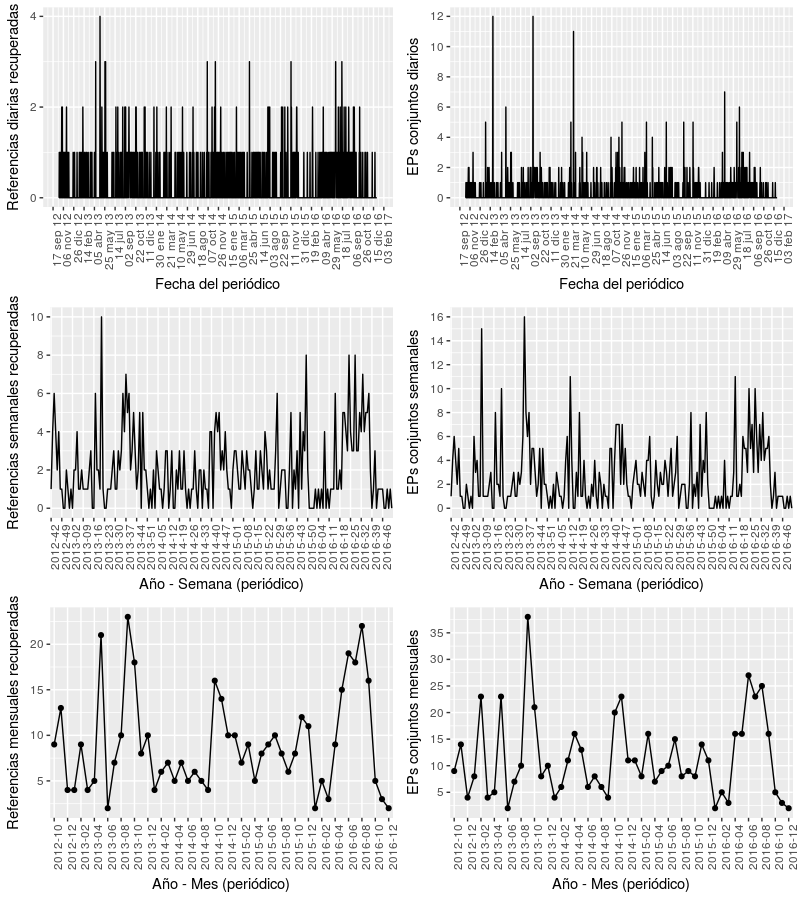
\includegraphics[scale=0.76]{img/3.1_serieT_fuentes.png}
\par\bigskip
\small Fuente: Elaboración propia.
\end{minipage}



%        BEGIN  EPs DE LARGA DURACIÓN                                                                                                                                    .
\subsection{Registro de eventos de protesta de larga duración}
\label{sec:EPs largos}


Otro aspecto que incentiva diferentes sesgos sobre algunas características en nuestros datos de coaliciones es la cobertura de eventos \emph{de larga duración}. 
Esto es, eventos de protesta que se sostienen por más de un día, algo que sucede a menudo en plantones, tomas de instalaciones, huelgas o paros de labores; los cuales pueden ser ``críticos porque ellos nos dicen las dinámicas de conflicto'' \citep[129]{2003_Wada_Tesis}. 

Dado que el valor noticioso de una protesta es relevante para ser cubierta por nuestra fuente, se debe considerar que los reportajes sobre eventos de larga duración usualmente refieren su inicio, fin o hitos; donde estos últimos, generalmente se acompañan de otras actividades de mayor trascendencia para nuestra fuente (como repertorios de protesta adicionales, nuevas demandas o reformulación de estrategias). 
En nuestra base de datos se consiguió identificar 40 eventos de este tipo, que obtuvieron en conjunto cobertura en 131 días; sin embargo, tal cobertura no se correlaciona con su duración aproximada ---de acuerdo a información complementaria hallada sobre tales manifestaciones en otros medios--- (ver figura \ref{3.2_epsLargos}). 


\hspace{-1.5em}\begin{minipage}{\linewidth}
\centering
\captionof{figure}{Duración aproximada y cobertura diaria de eventos de protesta de larga duración.} \label{3.2_epsLargos}
\hspace{-1.5em}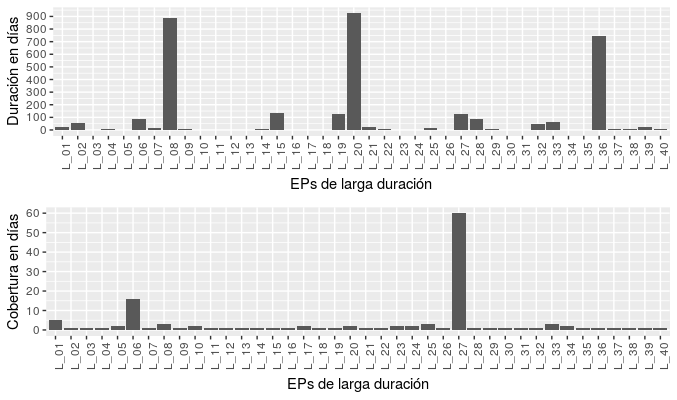
\includegraphics[scale=0.85]{img/3.2_epsLargos.png}
\par\bigskip
\small Fuente: Elaboración propia.
\end{minipage}\bigskip


Según \emph{La Jornada}, las coaliciones de eventos con una mayor duración aproximada\footnote{
    Tales eventos son tres plantones: 
    \begin{itemize}
    \setlength\itemsep{0.1em}
    \item \emph{L\_08}: de maestros afiliados a distintas secciones de la CNTE en el Monumento a la Revolución en la Ciudad de México, con una duración calculada de 890 días. 
    
    \item \emph{L\_20}: de ex-trabajadores de mexicana de aviación (respaldados por El Barzón) frente a los mostradores de la aerolínea, en la Terminal 1 del Aeropuerto Internacional de la Ciudad de México, con una duración documentada de 926 días (en realidad el plantón ---transformado en comercio informal--- se mantiene hasta el momento de escribir estas líneas; sin embargo, se calculó como fecha final el desalojo que sufrieron el 13 de enero de 2016 ---ver \url{http://www.jornada.unam.mx/2016/01/13/politica/014n1pol}---). 
    
    \item \emph{L\_20}: denominado "la dignidad y la resistencia", instalado en el zócalo de Chilpancingo por integrantes de la Coordinadora Estatal de Trabajadores de la Educación (Ceteg) y del Movimiento Popular de Guerrero (MPG) con una duración de 743 días, para exigir la presentación con vida de los 43 normalistas desaparecidos en Iguala en 2014.
    \end{itemize}
} 
usualmente no incorporaban otros repertorios de protesta en el mismo lugar en el que se registró el evento original. 
Si esto fuese cierto, con ello se reduciría la probabilidad que tales manifestaciones tenían para ser reportadas más de una vez en nuestra fuente; además, en otras coberturas no consideradas, se identificó a los manifestantes como un sólo grupo homogéneo, no como dos o más actores coparticipativos, por lo que nuestra submuestra descartó tales noticias relacionadas al no poder asegurar que todos los actores registrados hayan dado continuidad a su manifestación. 


En contraste, una serie de eventos destacables ---agrupados como \emph{L\_27} en la figura \ref{3.2_epsLargos}--- resulta ejemplar por la continua cobertura de sus actividades (de 60 días en total, para una duración calculada del evento de 128 días), su ocurrencia se da en el contexto del paro de labores llevado a cabo por las secciones 7 y 40 de la Coordinadora Nacional de Trabajadores de la Educación (CNTE)\footnote{
    Estas mismas secciones de la CNTE mantuvieron un paro de labores anterior ---agrupado como \emph{L\_06}--- donde también obtuvieron una buena cobertura (16 reportajes) en relación a su duración (89 días, aproximadamente).
}, 
donde se reportó usualmente más de un repertorio como forma de protesta. 

De forma general, corroboramos que no es posible asegurar una participación conjunta sostenida de los actores reportados en eventos de larga duración; aún en el seguimiento puntual que se da a algunos eventos de este tipo, se observa que los actores referidos cambian a lo largo del tiempo, lo que podría sugerir una dinámica en constante transformación. 
A su vez, basándonos sólo en los datos consignados es imposible conocer la continuidad de éstos y otros elementos relevantes como: demandas, repertorios u objetivos hacia quienes los manifestantes dirigen sus exigencias. 
Consecuentemente, tampoco realizamos ningún tratamiento adicional sobre aquellos reportes que nos ponen al día sobre la situación de coaliciones de eventos de larga duración. 


Más que un seguimiento continuo de la dinámica de la protesta colaborativa, reconocemos que: 
(i) cada registro en nuestros datos consignados toma sólo una instantánea incompleta sobre una coalición \emph{en un momento dado}; 
(ii) este registro discreto \emph{subestima y exagera a la vez la duración y posible impacto social real} de diversos eventos de larga duración; 
(iii) tales sesgos son dirigidos por eventuales \emph{criterios informativos} ---por su valor noticioso--- \emph{y subjetivos} ---donde algunas menciones reivindicativas sugiere una filiación ideológica con la fuente---; 
y (iv) en nuestra descripción de eventos de protesta ---y las redes que conforman--- dichas instantáneas se unen y confunden \emph{de manera equivalente} con coaliciones eventuales discretas. 







%        BEGIN  TIPO DE COBERTURA                                                                                                                                    .
\subsection{Cobertura temática}
\label{sec:cobertura_temas}

Revisamos en la tabla \ref{Secciones_Muestra_diarios} la clasificación que la propia fuente realiza de las noticias recabadas a fin de conocer un poco más el sesgo de su cobertura. 
Hallamos que (de forma consistente con la figura \ref{2.7_LaJornada_ElUniversal_secciones}) la gran mayoría de los reportajes sobre coaliciones de eventos es publicada en su sección \emph{política}.  
A partir de esta comprobación (y de acuerdo con otras particularidades referidas sobre \emph{La Jornada} en la sección \ref{sec:LaJornadaDiario}), podríamos conjeturar que las protestas colaborativas recabadas son transmitidas a través de una óptica editorial que enaltece su carácter de oposición política e impugnación gubernamental, ofreciendo a su vez limitados espacios suplementarios que permiten la divulgación de eventos conjuntos en otros ámbitos. 
Donde tal transmisión impregnará las relaciones sociales inferidas en nuestro análisis posterior. 


\begin{table}[!hbt]
\center
\footnotesize
\caption{Noticias clasificadas por sección en el diario.}
\label{Secciones_Muestra_diarios}
\begin{tabular}{ | l | c | } 
\hline
\textbf{Sección} & \textbf{Noticias} \\
\hline
Capital & 3\\
\hline
Cultura & 1\\
\hline
Economía & 2\\
\hline
Estados & 78\\
\hline
Política & 339\\
\hline
Sociedad & 44\\
\hline
\textbf{Total} & \textbf{467}\\
\hline
\end{tabular}
\par\bigskip
\caption*{\small Fuente: Elaboración propia.}
\vspace{-2em}
\end{table}


No obstante, este último recuento (aunque importante como perspectiva general) no revela los \emph{temas específicos} que tienen mayor trascendencia en nuestra fuente. 
Para verificar, aún de forma simple, la cobertura sostenida sobre ciertos asuntos concretos requerimos los textos periodísticos originales, para obtenerlos se empleo el script utilizado en la sección \ref{sec:Mediosnacionales_CoberturaComparativa}\footnote{
    Usado también allí para extraer textos periodísticos, a fin de realizar una comparación entre fuentes.
}. 


Una vez que se obtuvieron los textos, se eliminaron las \emph{palabras vacías}\footnote{
    Referidas anteriormente, en la subsección \ref{sec:sesgoMuestreo_keywords}, \nameref{sec:sesgoMuestreo_keywords}.
}, 
se filtraron palabras únicas por noticia y se calculó el número de reportajes en los que cada término aparece\footnote{
    Para este ejercicio se tomaron en consideración títulos, sumarios, pies de foto y cuerpos de cada noticia.
}. 
De los 200 términos con mayor presencia en los textos, se recuperan en la tabla \ref{TerminosComunesNoticias} cuarenta, que se consideran especialmente significativos por su relación a actores, lugares o hechos específicos en el periodo considerado; donde la frecuencia indicada refiere el número de noticias (de un total de 467) en los que cada término esta presente.
Asociamos una gran frecuencia en las palabras recuperadas a una mayor trascendencia (otorgada por la fuente) a los correspondientes asuntos públicos relacionados, que a su vez moldean nuestros datos sobre coaliciones de eventos. 



\begin{table}[!hbt]
\center
\footnotesize
\caption{Términos comunes en noticias consideradas.}
\label{TerminosComunesNoticias}
\begin{tabular}{ | c | l || c | l || c | l | } 
\hline
\textbf{Frecuencia} & \textbf{Término} & \textbf{Frecuencia} & \textbf{Término} & \textbf{Frecuencia} & \textbf{Término} \\
\hline
395 &  nacional & 156 &  estudiantes & 100 &  michoacán\\ \hline
361 &  trabajadores & 148 &  docentes & 95 &  magisterio\\ \hline
316 &  educación & 147 &  snte & 93 &  campesinos\\ \hline
304 &  coordinadora & 141 &  padres & 91 &  ceteg\\ \hline
273 &  maestros & 136 &  normalistas & 90 &  justicia\\ \hline
265 &  federal & 125 &  presidente & 88 &  mentores\\ \hline
254 &  sindicato & 123 &  tuxtla & 83 &  veracruz\\ \hline
252 &  reforma & 120 &  magisterial & 82 &  alumnos\\ \hline
224 &  profesores & 117 &  peña & 79 &  seguridad\\ \hline
208 &  guerrero & 110 &  chilpancingo & 79 &  normal\\ \hline
204 &  educativa & 109 &  congreso & 76 &  abrogación\\ \hline
191 &  chiapas & 103 &  desaparecidos & 73 &  lópez\\ \hline
165 &  cnte & 101 &  acapulco &  & \\ \hline
164 &  oaxaca & 101 &  ayotzinapa &  & \\ \hline
\end{tabular}
\par\bigskip
\caption*{\small Fuente: Elaboración propia.}
\vspace{-1em}
\end{table}



El reconocimiento particular de estos términos ---su correlación y un análisis de texto más minucioso--- puede ser de gran utilidad en el análisis dinámico de tendencias puntuales,  pues ``categorías altamente abstractas pueden oscurecer antes que aclarar cambios importantes'' \citep[162]{2003_Wada_Tesis}. 
No obstante, aún bajo un mero conteo, tales palabras parecen referir insistentemente dos temas trascendentales, con alto impacto en nuestros datos finales: 
(i) la \emph{reforma educativa}, promovida por el ejecutivo federal ---donde ``reforma educativa'' aparece en 188 noticias---; 
y (ii) la \emph{desaparición de los 43 normalistas de ayotzinapa}, en la que se involucró a diversos agentes gubernamentales ---con 101 coincidencias para ``ayotzinapa''\footnote{
    Antes de la desaparición de los normalistas, se aprecia que el término está presente. 
    Esto se debe a que los normalistas de esta comunidad (de forma similar a otros normalistas de escuelas rurales en el estado de Oaxaca)  tienen ya cierto historial en luchas sociales. 
    En particular, estas menciones suceden entre los meses de abril y mayo de 2013. 
    Dos noticias refieren su presencia en protestas cubiertas; y otras dos noticias recuerdan la muerte (por impacto de bala) de dos normalistas de esta comunidad, durante un desalojo policial de la Autopista del Sol, el 12 de diciembre de 2012. 
    Después de la desaparición de los 43 normalistas, el término tiene una carga semántica mucho más fuerte.
}---. 
Estos dos términos combinados aparecen en el 55.89\% de las noticias recuperadas, con una correlación mínima entre su ocurrencia, al coincidir únicamente en 28 de las 261 noticias donde se ubico alguno de los términos. 


\hspace{-1em}\begin{minipage}{\linewidth}
\centering 
\captionof{figure}{Ocurrencia de términos relevantes en noticias muestreadas.} \label{3.3_tendenciasTerminos}
\hspace{-1.2em}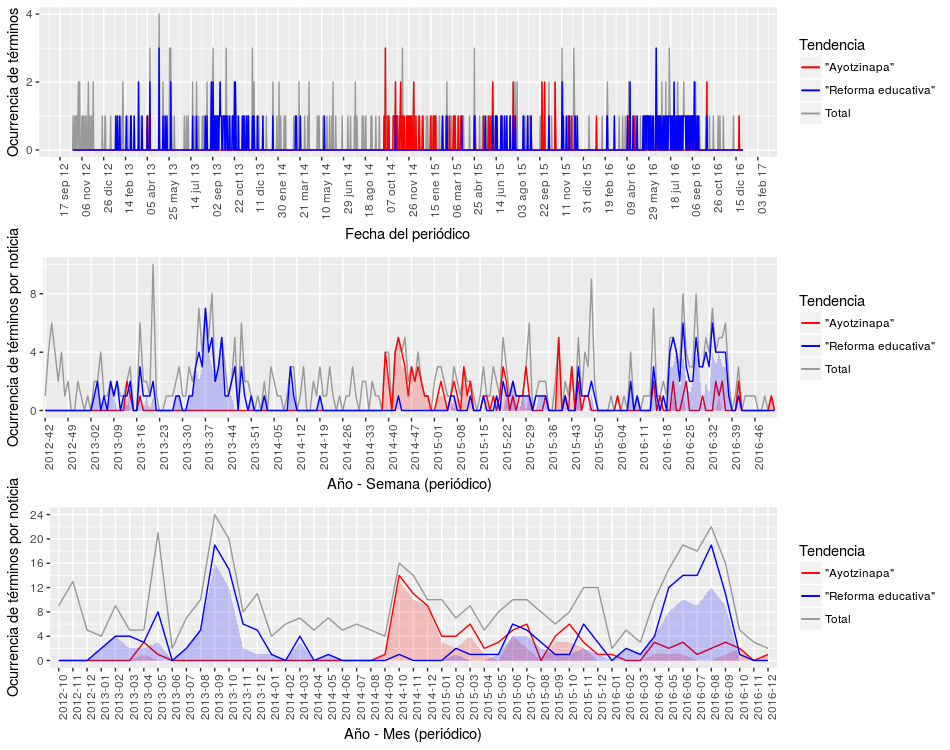
\includegraphics[scale=0.62]{img/3.3_tendenciasTerminos.png}
\par
\small Fuente: Elaboración propia.
\end{minipage}\bigskip


Para comprobar el tipo de presencia longitudinal que tienen estos temas, se presenta en la figura \ref{3.3_tendenciasTerminos} series de tiempo relacionadas a cada término ---dada la cobertura de las protestas recabadas, en distintas agrupaciones---; donde la mayor parte de periodos con una gran cantidad de reportajes están relacionados a la presencia de alguno de estos temas. 
Ya que su mención puede ocupar una posición principal o secundaria en el diario, se representa en un área bajo la tendencia de cada término la ocurrencia que cada uno de ellos tuvo en lugares relevantes de una noticia\footnote{
    Para ello, se consideró sólo el título, los sumarios y la primer quinta parte del cuerpo de una noticia.
}; 
en general, se distingue una presencia importante de los términos \emph{ayotzinapa} y \emph{reforma educativa} en el 69.15\% y 64.36\% de los casos, respectivamente. 





Es significativo que al referirse a ciertos movimientos sociales, ocasionalmente hallamos noticias enlazadas en \emph{La Jornada} bajo ``\emph{series}'', que ofrecen actualizaciones sobre algunas temáticas (y movilizaciones) de especial importancia para el diario.  
En las noticias recopiladas, las series de mayor frecuencia también son aquellas hacen referencia al movimiento de maestros sindicalizados (8 series) y a la desaparición de los 43 normalistas (6 series). 
Su aparición recurrente y el nombre con el que se enaltece estos temas evidencian el sesgo informativo con el que se plasman tales noticias, afines a su línea editorial\footnote{
   Hallamos, para el caso de la reforma educativa, series como: ``\emph{evaluación desairada}'', ``\emph{insurgencia magisterial}'', ``\emph{lucha magisterial}'' o ``\emph{resistencia magisterial}''. 
   Y, en el caso de los 43 normalistas: ``\emph{a tres meses de la tragedia}'', ``\emph{Ayotzinapa, la herida abierta}'', ``\emph{caída de la pareja imperial}'', ``\emph{crisis en Guerrero}'' o ``\emph{la indignación}''. 
}. 


Aunque estas tendencias nos ofrecen una guía sobre la subsistencia de dos coyunturas en las notas sobre protestas que recuperamos, tenemos presente que no necesariamente existe una causalidad lineal entre la persistencia de estos temas en el diario y una ocurrencia extendida y uniforme del tipo de coaliciones de eventos en las que centramos nuestra atención\footnote{
    A pesar de que (como se comprueba en la figura \ref{3.17_serieDemandas}) una gran cantidad de demandas en las protestas recabadas sí pueden ser vinculadas directamente a estos temas. 
}. 
Paradójicamente, es debido a esta misma relevancia mediática que aún las \emph{principales motivaciones y demandas} en los sucesos involucrados en nuestra evidencia pueden no ser consecuencia directa de estos contextos. 
Los manifestantes que conforman coaliciones 
pueden circunscribir su propio discurso ---resultando acentuado por la fuente--- a uno de estos temas únicamente con el objetivo de obtener una mayor validez, reconocimiento o ante la posibilidad de crear alianzas amplias a partir de una base común. 
Suponemos que aunque exista cierta relevancia objetiva en estos asuntos dentro de las coaliciones en eventos, su amplio alcance mediático plasmado en nuestros datos
es el efecto circunstancial de sesgos añadidos, principalmente achacados a olas de interés periodístico dentro de la \emph{La Jornada}, que en conjunto suponemos como \emph{ciclos de atención mediática}, que enfatizan y soslayan hechos sociales emblemáticos. 


Existe una gran diversidad de acontecimientos adicionales que no tenemos intención de minimizar; la vida política y social del país en el periodo analizado no se reduce a los dos temas antes referidos, así como tampoco a los temas que han podido ser captados en nuestra base de datos. 
Empero, bajo una perspectiva panorámica de nuestra evidencia y por la trascendencia que los acontecimientos hasta ahora considerados parecen tener en nuestra fuente, centramos de momento nuestra atención en ellos. 
De este modo, a continuación se presentan ---de forma breve--- sus cronologías\footnote{
    Extraídas principalmente de cronologías anuales, elaboradas por el LAOMS, donde se plasmaron aquellos hechos sociales con presencia mediática, que se consideraron más trascendentales para el fenómeno de la protesta en el país. 
}, donde se comprueba que los periodos con mayor cobertura (en las noticias recuperadas) corresponden a fechas clave dentro de estos movimientos. 




\subsubsection{Reforma educativa}
\label{sec:ReformaEducativa}

\begin{itemize}
    \setlength\itemsep{0em}
    \item \emph{diciembre de 2012:} Las reformas a los artículos 3 y 73 constitucionales son enviada por el presidente, resultando aprobadas el día 20.
    \item \emph{febrero de 2013:} Se publica la reforma educativa en el Diario Oficial de la Federación el día 26.
    \item \emph{agosto de 2013:} El día 13, el presidente envía al Congreso de la Unión tres iniciativas de ley para concretar la reforma educativa: (i) reforma a la Ley General de Educación, (ii) Ley del Instituto Nacional para la Evaluación de la Educación (INEE) y (iii) Ley General del Servicio Profesional Docente. 
    El día 23 se aprueba la reforma a la ley General de  Educación y la Ley del INEE.
    \item \emph{septiembre de 2013:} El día 3 se aprueba la Ley General del Servicio  Profesional Docente. 
    El día 10 se promulgan las tres leyes secundarias de la  reforma educativa, se publican en el Diario Oficial de la Federación al día siguiente. 
    \item \emph{junio de 2015:} Inicia en algunos estados el proceso de la Evaluación del Servicio Profesional Docente. 
    \item \emph{julio de 2015:} El día 21 se anuncia la desaparición del Instituto Estatal de Educación Pública de Oaxaca (IEEPO), dependencia estatal controlada por la CNTE. Para el día 4 la Secretaría de Educación Publica (SEP) logró completar la Evaluación del Servicio Profesional Docente a nivel Medio Superior en 29 estados del país.
    \item \emph{mayo de 2016:} El día 15 la CNTE inicia un paro de labores nacional indefinido, en protesta por la implementación de la reforma educativa, los estados más afectados son Chiapas, Oaxaca, Michoacán y Guerrero. El 19 se anuncia el despido de 4 mil 253 maestros disidentes no afiliados al SNTE.
    \item \emph{junio de 2016:} El día 19, durante un desalojo (luego de varios días de bloqueos en carreteras de la entidad) al bloqueo que integrantes de la CNTE mantenían en la autopista Oaxaca-Cuacnopalan, a la altura del municipio mixteco de Asunción Nochixtlán, murieron ocho personas y un centenar más fueron heridos.
    \item \emph{septiembre de 2016:} Se levanta paulatinamente el paro de labores de la CNTE, tras lograr acuerdos temporales con autoridades.
\end{itemize}

\subsubsection{Ayotzinapa}
\label{sec:ayotzinapa}

\begin{itemize}
    \setlength\itemsep{0em}
    \item \emph{septiembre de 2014:} Durante la noche del día 26 un grupo de normalistas, a bordo de tres autobuses, es atacado por policías estatales, dejando a tres personas muertas y 43 estudiantes desaparecidos.
    \item \emph{octubre de 2014:} La PGR investiga a la esposa del alcalde de iguala por vínculos con el grupo criminal \emph{Guerreros Unidos}. 
    El día 15 la PGR informa sobre peritajes en las primeras cinco (de catorce) fosas clandestinas localizadas, determinaron que ninguno de los 28 cuerpos localizados corresponde a los estudiantes de la Escuela Normal Rural de Ayotzinapa.
    \item \emph{noviembre de 2014:} El día 4 detienen al ex-alcalde de Iguala, José Luis Abarca Velázquez y a su esposa. 
    El día 7 presenta la PGR su informe, donde asegura que los 43 normalistas de Ayotzinapa habrían sido asesinados y calcinados en el basurero del municipio de Cocula, según los testimonios de tres participantes materiales en el presunto multihomicidio. 
    \item \emph{septiembre de 2015:} El día 6 presenta el Grupo Interdisciplinario de Expertos Independientes (GIEI) su informe sobre los sucesos en ayotzinapa, indican que no hay evidencia de que los 43 normalistas hayan muerto quemados en el basurero de Cocula; la PGR abre otras líneas de investigación.
\end{itemize}


%        BEGIN  REPRESENTACIÓN GEOGRÁFICA DE EVENTOS                                                                                                                         .
\subsection{Representación geográfica de eventos}
\label{sec:representacion_geo}

Siguiendo con nuestra discusión de la sección \ref{sec:cobertura}, ya que nuestro criterio para identificar protestas a nivel municipal puede afectar la representación geográfica original de las noticias recabadas ---reproduciendo eventos casi idénticos en diversos municipios---, presentamos las frecuencias asociadas a menciones únicas a protestas en un estado por noticia (figura \ref{3.4_noticiasEstados}) y la distribución a nivel estatal del conteo agregado de eventos en nuestra base de datos (figura \ref{3.5_epsEstados}) para efectos de comparación.  


\hspace{-1em}\begin{minipage}{\linewidth}
\centering
\captionof{figure}{Menciones únicas de estados en noticias consideradas.} \label{3.4_noticiasEstados}
\hspace{-1.5em}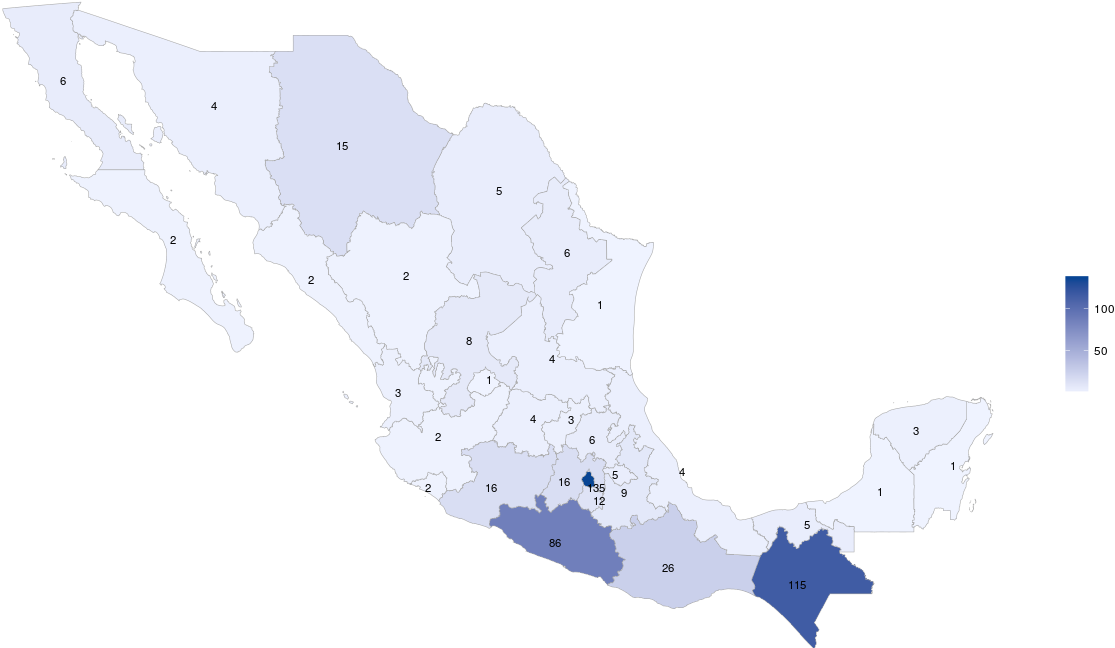
\includegraphics[scale=0.55]{img/3.4_noticiasEstados.png}
\par
\small Fuente: Elaboración propia.
\end{minipage}\bigskip

Donde ratificamos la asimetría en el peso de este sesgo, ya que la mayor parte de estados con poca presencia en nuestros datos permanece sin cambios relevantes entre el número de eventos y artículos relacionados ---salvo en el caso de Chihuahua---; mientras que, por otro lado, hay una gran redundancia de protestas en sitios con una mayor cobertura (es decir, en los estados de Chiapas, Guerrero y Ciudad de México). 
Deducimos que, tanto la aglomeración de reportajes, como la sobrerrepresentación territorial de eventos referidos en ciertos estados, son impulsados por el sesgo con el que nuestra fuente enfatiza coaliciones regionales simultáneas o análogas, producidas en áreas donde el diario tiene una mayor presencia. 



\hspace{-1em}\begin{minipage}{\linewidth}
\centering
\captionof{figure}{Eventos de protesta --- agregación estatal.} \label{3.5_epsEstados}
\hspace{-1.5em}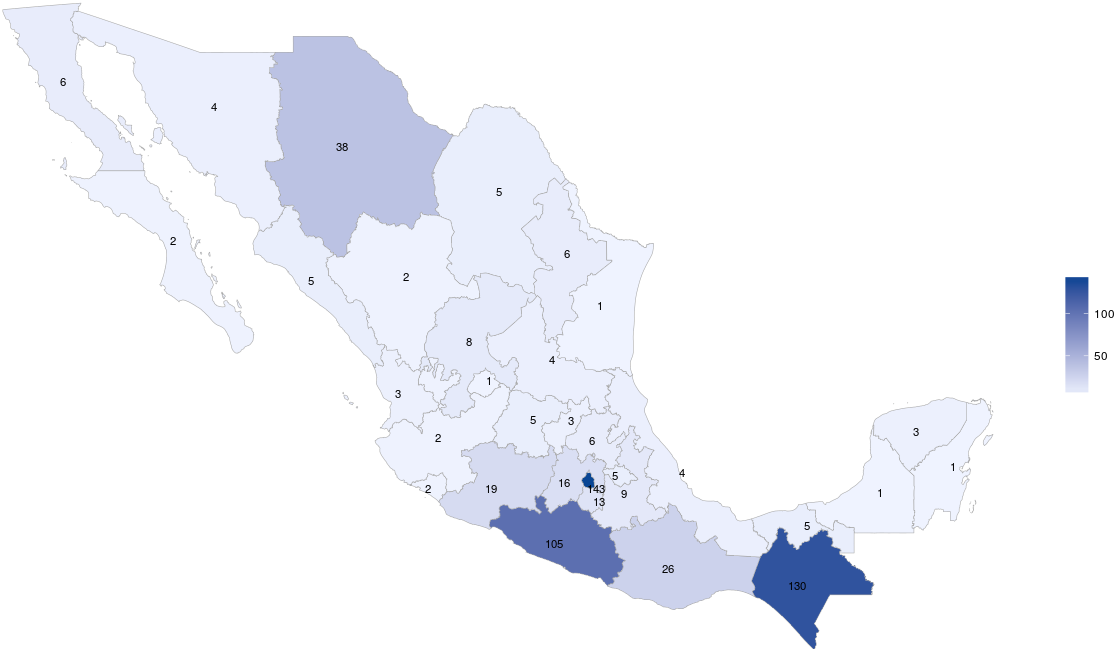
\includegraphics[scale=0.55]{img/3.5_epsEstados.png}
\par
\small Fuente: Elaboración propia.
\end{minipage}\bigskip

La ciudad de México registra 143 eventos (más que cualquier otro estado) lo cual se explica por dos causas: en primer lugar, dado que ahí se edita nuestra fuente de referencia y en segundo, debido a la alta concentración de recursos políticos en el país (la mayor parte de los edificios gubernamentales federales se encuentra allí). 
En segundo sitio está Chiapas, donde buena parte de sus 130 eventos de protesta, están ligados a la reforma educativa (cuya relevancia potencial es mostrada en la figura \ref{3.3_tendenciasTerminos}); además, en este estado se mantienen dos de las secciones de la CNTE con mayores colaboraciones registradas en eventos de protesta ---dada una fuerte atención mediática en el último periodo de lucha contra la reforma educativa, que reproduce varios eventos enlazados (ver sección \ref{sec:EPs largos})---. 
El estado de Guerrero está en tercer sitio, con 105 protestas; lo cual es comprensible ya que en dicho estado se produjo la desaparición de los 43 normalistas de Ayotzinapa; además, en este estado nuestra fuente mantiene una edición local y debido a ello le resultaría más sencillo dar un seguimiento cercano a los conflictos. 
Con una gran diferencia, el estado de Chihuahua es el siguiente (con 38 protestas en total) donde 26 eventos fueron deducidos ---según los criterios adoptados-- a partir de 4 noticias, las cuales reportaron manifestaciones simultáneas en diferentes municipios, por lo que su sobrerrepresentación está hasta cierto punto comprometida por la forma en la que se ha consignado información. 
Finalmente, Oaxaca y Michoacán (estados donde también se reportaron en mayor medida eventos de protesta sobre la reforma educativa y donde existe una gran influencia de asociaciones nacionales de maestros) tienen cierta cobertura significativa. 
El resto de los estados registra como promedio de eventos 4.69 y como mediana 4. 



De lo anterior, inferimos que los sesgos circunstanciales, geográficos, editoriales y de consignación se entrelazan y retroalimentan a menudo, reduciendo la calidad objetiva de nuestra muestra. 
Aunque no somos capaces de reconocer la incidencia exacta de cada sesgo, esta identificación nos permite hacer suposiciones más informadas respecto a las características de las coaliciones analizadas y las posibles estructuras sociales en las que se sostienen. 


Para ahondar en la distribución geográfica de eventos, consideramos significativa la agregación municipal (al ser una referencia de organización territorial, así como de división política y administrativa local), donde la desproporcionalidad de eventos es aún mayor\footnote{
    Ya que sólo se documentaron coaliciones de eventos en 116 municipios de 2,457 en el país (el número de municipios en México no es consistente en el tiempo y tiende a incrementarse debido a legislaciones estatales, la lista de municipios fue recuperada del paquete \emph{inegiR}, del lenguaje de programación \emph{R}). 
    Por otro lado, cabe aclarar que existe una pérdida de dos eventos, ya que en dichos casos sólo se pudo deducir desde la fuente el estado donde ocurrieron las protestas (Quintana Roo y Chiapas). 
    
} 
(ver figuras \ref{3.6_epsMunicipios} y \ref{3.7_epsMunicipiosfreq}), de modo que tan sólo cuatro municipios del país\footnote{
    Tuxtla Gutiérrez en Chiapas (100 EPs), Cuauhtémoc en la Ciudad de México (99 EPs), Chilpancingo de los Bravo en Guerrero (44 EPs) y Acapulco de Juárez (33 EPs).
} concentran 276 coaliciones de eventos (47.34\% del total). 

\hspace{-1em}\begin{minipage}{\linewidth}
\centering
\captionof{figure}{Eventos de protesta --- agregación municipal.} \label{3.6_epsMunicipios}
\hspace{-1.5em}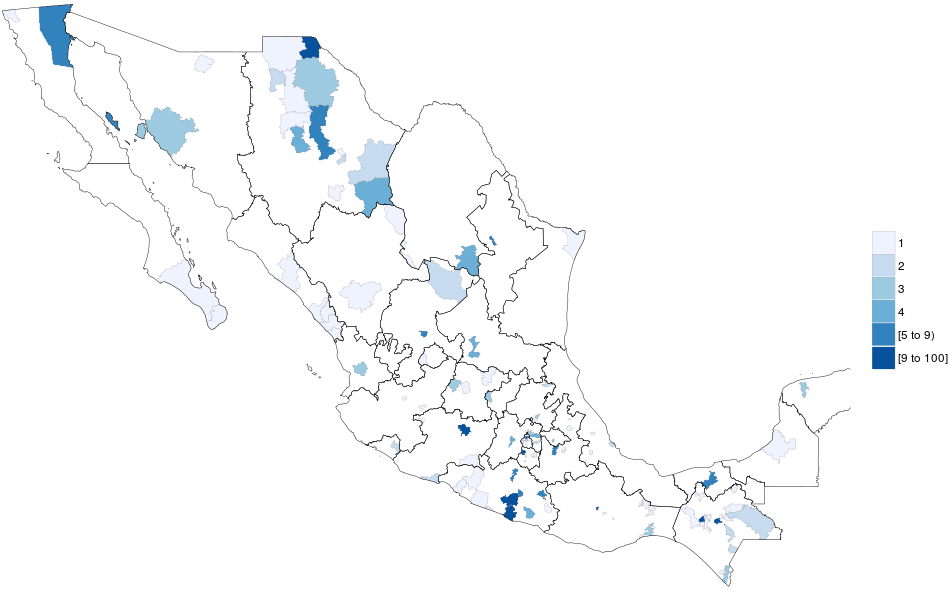
\includegraphics[scale=0.63]{img/3.6_epsMunicipios.png}
\par
\small Fuente: Elaboración propia.
\end{minipage}\bigskip

Los municipios donde se registraron más protestas son principalmente capitales estatales y áreas urbanas con una gran densidad de población; lo que podría implicar una subrepresentación de poblaciones rurales y una visión particularmente limitada sobre las coaliciones de eventos en el país. 

\hspace{-1em}\begin{minipage}{\linewidth}
\centering
\captionof{figure}{Distribución agregada de protestas en municipios.} \label{3.7_epsMunicipiosfreq}
\hspace{-1.5em}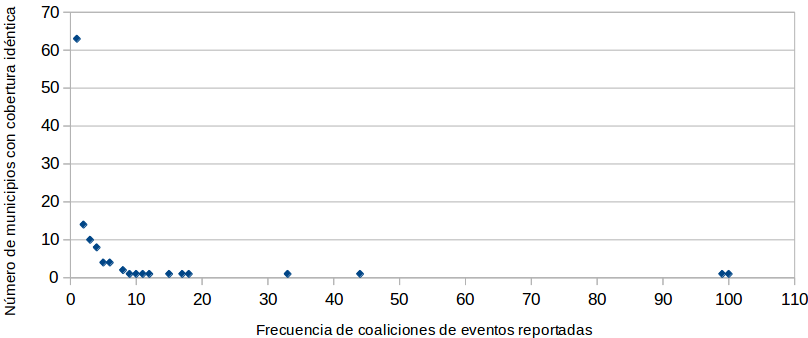
\includegraphics[scale=0.54]{img/3.7_epsMunicipiosfreq.png}
\par\bigskip
\small Fuente: Elaboración propia.
\end{minipage}\bigskip


Una representación aún más específica sobre la distribución geográfica de eventos puede ser conseguida por su geolocalización\footnote{
    A pesar de que se ha hecho el esfuerzo de obtener esta información, tenemos dos problemas: en primer lugar, la fuente puede no reportar con precisión el lugar en el que se produce el evento, en segundo lugar, aún si la fuente reporta los lugares exactos, el criterio de agregación municipal del esquema de codificación impide una representación precisa para más de una ubicación descrita.
    Para el primer caso, ya que hemos obtenido la localización en la mayoría de los eventos hasta el nivel municipal, consideramos que una aproximación al centro del municipio (obtenida por la API \emph{ggmap} de \emph{R}) es suficiente para describir patrones generales a nivel nacional.
    Para el segundo caso, el esquema de codificación considera que si una manifestación se desplaza (como en el caso de las marchas) entonces se indica el lugar en el que la protestas se detiene, o el sitio en el que esta se reporta (si se trata de una rodada o caravana); por otro lado, cuando la fuente reportó varios lugares, se eligió el sitio más específico o el primero en ser mencionado en su defecto.
}. 
Una aproximación al respecto es mostrada en la figura \ref{3.8_epsGeolocalizacion}, donde se indican además algunos de los principales repertorios de protesta consignados y que potencialmente tienen un impacto distinguible en diferentes partes del país\footnote{
    Ya que una buena parte de las protestas registran más de un repertorio (aquellos indicados en el \nameref{Anexo_RepertoriosPacificos}) se utiliza para cada geolocalización sólo uno de ellos, considerado de mayor impacto y utilizado como referencia, dando preferencia a: 
    (i) Bloqueos, 
    (ii) Plantones, 
    (iii) Marchas (incluyendo anuales y conmemorativas), 
    (iv) Mítines, 
    (v) Paros de labores, 
    (vi) Tomas de instalaciones, 
    (vii) Caravanas y 
    (viii) Repertorios Pacíficos Indeterminados. 
    Si ninguna de las protestas incluye alguna de estas tácticas, se etiquetó la ubicación como \emph{Otro}; además, se indica como \emph{Varios}, aquellos lugares que incluyeron más de una protesta (ya sea debido a que sólo se pudo determinar el municipio o porque se trata de un lugar específico en el que se registran varias manifestaciones) de forma que no es posible asignar sólo un repertorio de referencia. 
}. 


Nuestro mapeo de manifestaciones colaborativas aglomera y superpone múltiples eventos, demostrando que la concentración de manifestaciones (aún dentro de municipios acotados) es poco heterogénea y sólo podría considerarse ligada (dentro de las limitaciones antes descritas) a ciertos espacios públicos. 
Por su parte, tomando con reserva la información presentada sobre repertorios (dadas las precauciones anticipadas sobre la consistencia de su consignación ---ver sección \ref{sec:NotiMuestreo}---), observamos que carreteras en el sur del país sufrieron una mayor cantidad de bloqueos ---varios de ellos promovidos por maestros disidentes---, mientras que las marchas fueron repertorios comunes en ciudades y poblaciones en gran parte de los territorios considerados. 
Finalmente, por el sesgo antes descrito en Chihuahua, se aprecia la homogeneización de los repertorios en este estado. 


\hspace{-2em}\begin{minipage}{\linewidth}
\centering
\captionof{figure}{Coaliciones de eventos --- Geolocalización aproximada.} \label{3.8_epsGeolocalizacion}
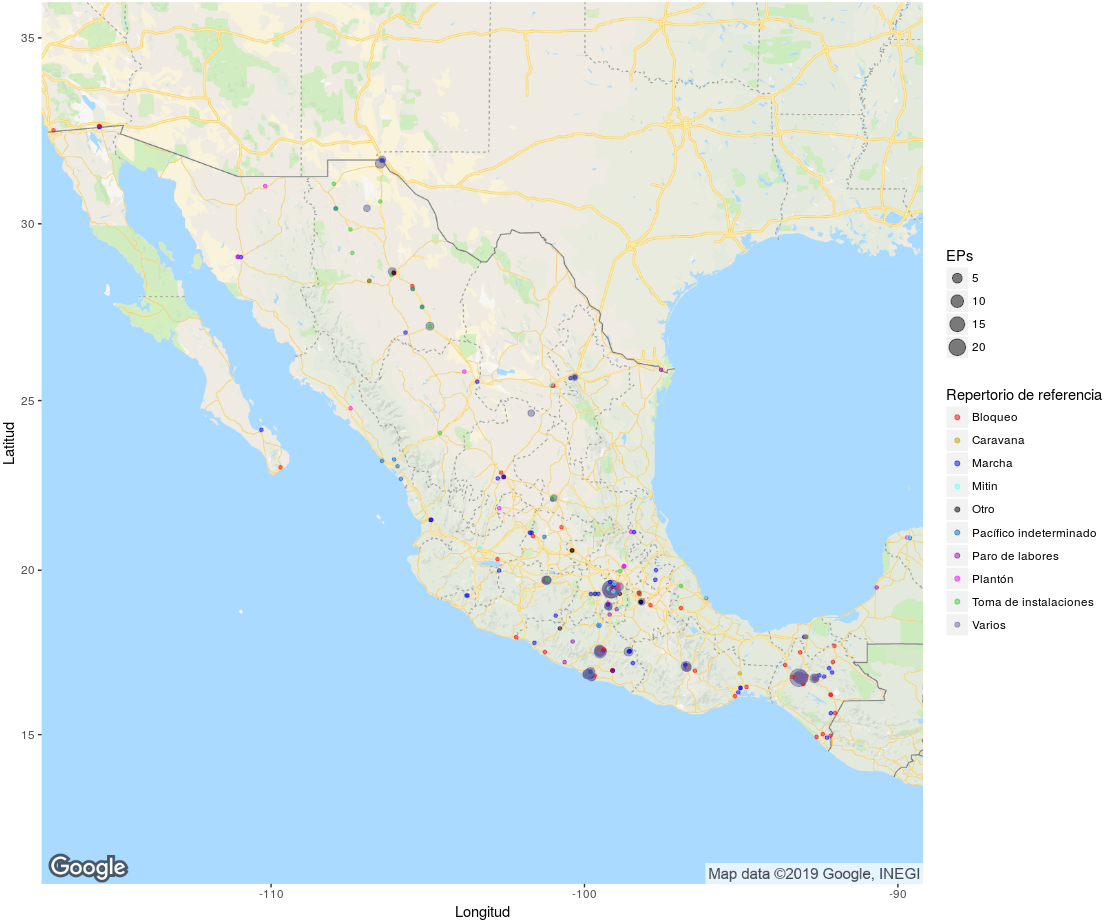
\includegraphics[scale=0.53]{img/3.8_epsGeolocalizacion.png}
\par\bigskip
\small Fuente: Elaboración propia.
\end{minipage}\bigskip


Concentrándonos en las cuatro ciudades donde se han registrado más eventos (Ciudad de México, Chilpancingo de los Bravo, Tuxtla Gutiérrez, y Acapulco de Juárez), mostramos en la figura \ref{3.9_epsGeoLocal} los lugares específicos donde se han podido detectar coaliciones de eventos. 
Los puntos carreteros que conectan estas ciudades con el resto del país son objetivos evidentes de manifestantes; otros sitios comunes implican calles, plazas y avenidas principales además de oficinas gubernamentales y en algunos casos aeropuertos\footnote{
    En la ciudad de México, los lugares con mayores protestas son: la Plaza de la Constitución (24 EPs), la Secretaría de Gobernación (21 EPs), las oficinas de la SAGARPA (12 EPs), el Senado de la República y el Monumento a la Revolución (8 EPs cada uno). 
    En Tuxtla Gutierrez: las oficinas de la Secretaría de Educación Estatal (12 EPs), la Plaza Mayor (6 EPs) y la Torre de PEMEX (5 EPs). 
    En Chilpancingo: el Congreso del Estado (9 EPs), el Zócalo y la Autopista del Sol (5 EPs cada uno). 
    En Acapulco: la Av. Costera Miguel Alemán (5 EPs), el Palacio Municipal y la Caseta de La Venta (4 EPs cada uno).
}.


\hspace{-1em}\begin{minipage}{\linewidth}
\centering
\captionof{figure}{Geolocalización de coaliciones en ciudades con mayor representación mediática.} \label{3.9_epsGeoLocal}
\hspace{-2em}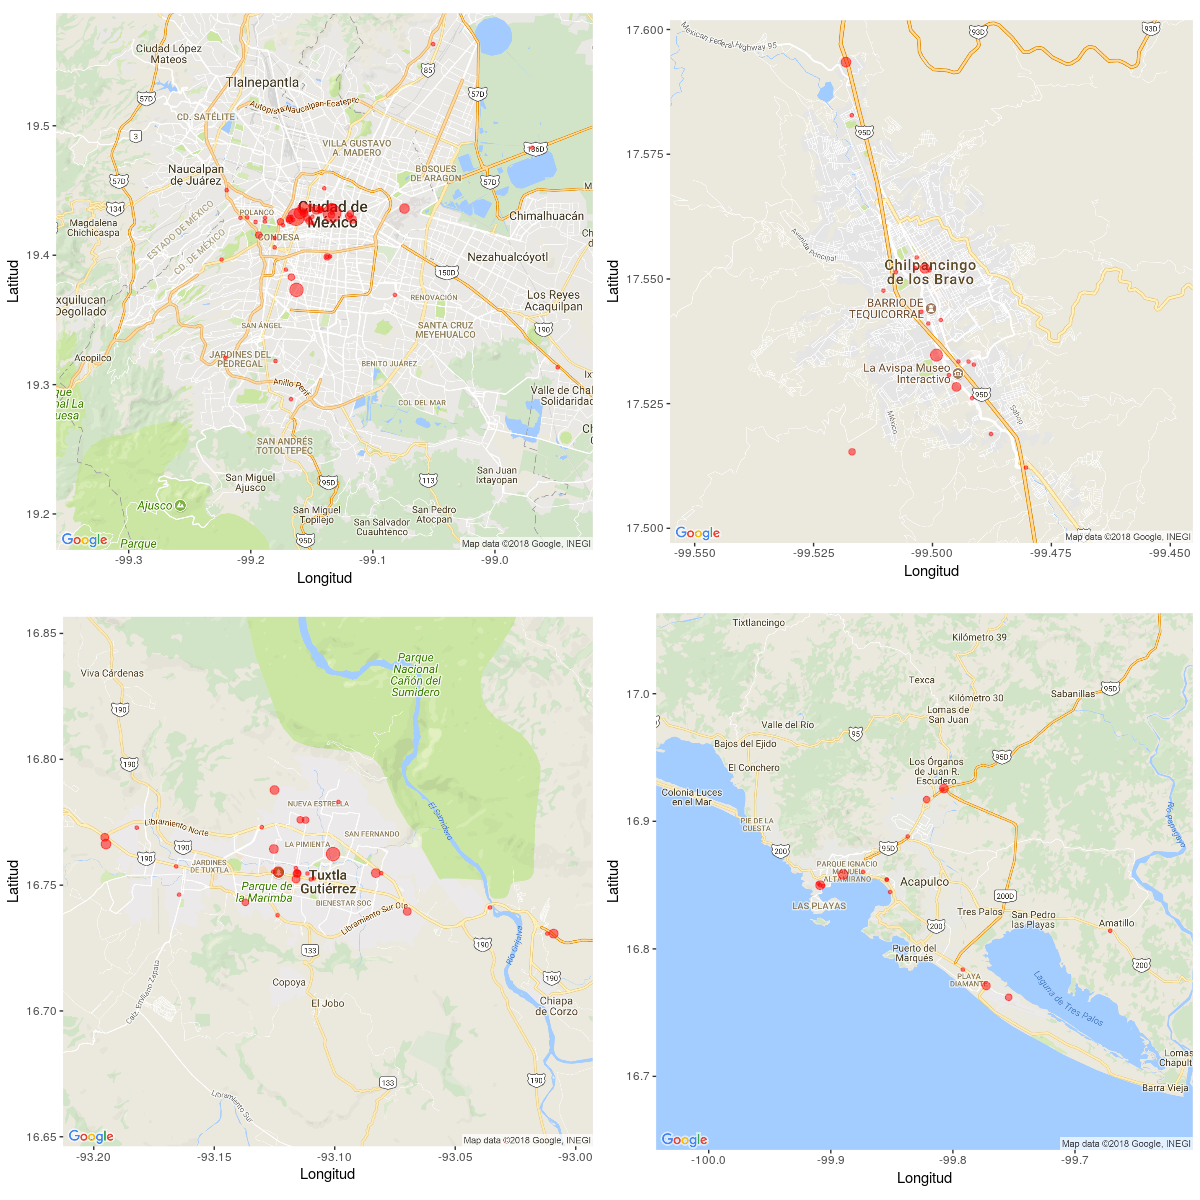
\includegraphics[scale=0.5]{img/3.9_epsGeoLocal.png}
\par
\small Fuente: Elaboración propia.
\end{minipage}\bigskip

Conjeturamos que los lugares donde se protesta son elegidos de forma estratégica, por ser oficinas de alguna dependencia que puede resolver sus demandas; pero también por ser instituciones con mayor poder o reconocimiento simbólico. 
También que otros lugares públicos son elegidos (e implican una mayor probabilidad de cobertura) por el impacto que provoca la manifestación, por ser emblemáticos o por su importancia relativa o contextual. 
Lo cual ya ha sido propuesto para amplias localidades urbanas como las que se consideran: 
\begin{center}
    \begin{minipage}{0.9\linewidth}
        {\setlength{\parindent}{12pt}\small
	     En la ciudad, los manifestantes se desplazan en espacios estratégicos para hacer visibles las dimensiones de la movilización y sus demandas, uno de los objetivos es llegar al frente de las edificaciones que albergan las instituciones responsables de resolver sus demandas. 
	     Así mismo, el desplazamiento en las calles de la ciudad, generalmente, se realiza en sendas y nodos emblemáticos y de mayor afluencia de transeúntes y transporte público y privado, buscan las edificaciones e iconos simbólicos que contribuyen a que la movilización sea observada por la mayor parte de los pobladores. 
	     Esta relación expresa simbólicamente, al espacio de las sendas y los nodos en ``el espacio público urbano sede de formas plurales de expresión ciudadana y de formas distintas de apropiación colectiva de la ciudad... la ciudad es el espacio público al ser espacio de lugares, sedes de formas diversas de relación, de acción, de expresión y de participación en asuntos de interés ciudadano...'' (Ramirez, 2003: 36-37).  \normalsize \citep[247--248]{2015_Nicolasa_MassMedia}.
        }
    \end{minipage}
\end{center}



%        BEGIN  SECCIÓN 3.2.                                                                                                                                    .                                                                                                                                                               .                                          CARACTERÍSTICAS                                                                                                      .                                                                                                                                           .                                                                                                                                                               .
\section{Características en coaliciones cuantificadas}
\label{sec:CaracterísticasCuantificadas}

Por el reconocimiento de sesgos distintivos ---ideológicos, geográficos, organizativos y editoriales, abordados en las secciones \ref{sec:Mediosnacionales} y \ref{sec:LaJornadaDiario}--- de \emph{La Jornada} en relación a otros medios periodísticos, deducimos que la irregular cobertura que hemos mostrado en la sección anterior (territorial, temática y longitudinal) dada nuestra muestra sobre noticias, implica \emph{representaciones intencionalmente acotadas sobre coaliciones nacionales}; suscitadas por ciclos de atención mediática y ampliando su efecto al superponerse a algunas decisiones metodológicas discriminatorias adoptadas. 
Ya que nuestros datos se construyen a partir de \emph{eventos} (o más específicamente de \emph{coaliciones de eventos}), la identificación y consignación de varios atributos \emph{desde esta unidad de análisis}, ponderada por el medio discrecionalmente, arrastrará inercialmente los sesgos de cobertura descritos, añadiendo otros que contribuyen a mediciones asimétricas. 


Como unidad social que se deriva de un hecho público difundido mediáticamente, el \emph{evento de protesta} sirve como enlace social común, con la capacidad de articular actores, demandas repertorios, objetivos y respuestas (entre otras características razonables, definidas en un diseño de investigación). 
De tales atributos, consideramos para nuestro análisis de redes posterior a \emph{actores} y \emph{demandas} como \emph{unidades sociales} interrelacionadas, que son trascendentes para estudiar las coaliciones de eventos muestreadas y su representación mediática. 
El énfasis con el que describimos ambos tipos de unidades pretende dar cuenta de su trascendencia posterior. 


Por otra parte, aunque no se utilizan en nuestro análisis de redes, también consideramos relevante reparar en otras características recabadas sobre eventos, por su aporte contextual y una mejor comprensión potencial sobre la constitución de las coaliciones recabadas, cuya naturaleza moldea posteriores estructuras sociales inferidas. 
Estos atributos son:
\begin{description}
    \setlength\itemsep{0em}
    \item[Repertorios de protesta.] 
    Que sugieren el grado de organización y planeación de eventos, precisando \emph{cómo} se actúa. 
    De esta forma, si un balance general informa que repertorios que requieren un gran número de manifestantes (como caravanas, marchas, huelgas y paros de labores) son mayoritariamente utilizados, podríamos asumir que las relaciones inferidas (colaborativas y discursivas) entre manifestantes implican mejores marcos constitutivos; por el contrario, repertorios violentos o cuya práctica no involucre un gran compromiso de recursos humanos o materiales (como brigadeos, bloqueos, toma de casetas, boicots o huelgas de hambre) podrían augurar una menor sistematización en la conformación de eventos. 
    \item[Objetivos.] 
    Dado que la línea editorial en nuestra fuente tiene un evidente sesgo político, resultará significativo comprobar si esto supone un reconocimiento uniforme sobre el tipo de objetivos  (principalmente gubernamentales) ante los cuales los manifestantes dirigen sus demandas. 
    La diversificación o uniformidad de contendientes también puede especificar el contexto en el que se desarrolla la protesta colaborativa: formando frentes comunes ante adversarios consistentemente confrontados, o dispersando los objetivos de sus exigencias en contextos alternados. 
    \item[Respuestas a la protesta.]  
    Ya que ---como se verá posteriormente--- gran parte de los actores confrontados son figuras gubernamentales, las respuestas inmediatas registradas en nuestra fuente pueden reflejar la dinámica de las interacciones analizadas, al mostrar las condiciones (represivas, negociarías o simplemente de garantía ante su derecho a la protesta) bajo las cuales se desarrollan estas coaliciones.
\end{description}



% BEGIN  DESCRIPCIÓN DE ACTORES                                                      
\subsection{Actores}
\label{sec:actores}

Nuestra submuestra fue seleccionada específicamente con el objetivo de filtrar protestas en las que dos o más actores (reconocidos y organizados hasta cierto punto) coparticiparon alrededor de movimientos sociales reconocidos. 
En un entorno plural, esto supondría una alta injerencia de sectores y narrativas heterogéneas, más allá de las que se pueden asociar a las luchas individuales vinculadas a actores colectivos únicos. 
Sin embargo, en nuestros datos la mayor parte de manifestaciones sólo se produce entre unas pocas organizaciones colaborativas; además, la desproporcionalidad en la frecuencia de sus coaliciones reportadas es mayor de la esperada, reduciendo considerablemente la variedad de nuestros datos.


Se identificaron 432 actores, con 1,780 coparticipaciones en total, distribuidas alrededor de 583 coaliciones de eventos de protesta, como se observa en la figura \ref{3.10_distribucionActores}. 
Algunos de estos actores podrían ser agrupados en un nivel superior debido a que se registran secciones subalternas (no necesariamente subordinadas) de otro actor, lo cual sucede en sindicatos, redes, campañas u organizaciones paraguas; pero ya que no en todos los casos la relación es clara, ya que existe cierta independencia entre ellos y debido a que esto desviaría en gran medida la representación original sobre los actores colectivos en nuestra fuente, no realizamos tal agregación\footnote{
    Aunque esta sería posible con información adicional, que presentara evidencia sobre los vínculos formales entre actores. 
    Una excepción que hemos hecho ha sido para las secciones del \emph{Sindicato Nacional de Trabajadores de la Educación} (SNTE), debido a que algunas de ellas se encuentran dominadas por la \emph{Coordinadora Nacional de Trabajadores de la Educación} (CNTE) ---por ejemplo: la sección 22 (en Oaxaca), las secciones 7 y 40 (en Chiapas), la sección 14 (en Guerrero) y la 18 (en Michoacán) entre otras---; ya que su identificación es regional o por número de sección, es usual que nuestra fuente se refiera indistintamente al SNTE (agrupación gremial) o a la CNTE (organización disidente de bases, cuyos agremiados siguen formando parte del SNTE) por lo que se homologó su mención por número de sección cuando tal identificación fue posible y se ha podido reconocer el dominio de una organización sobre otra.
}. 




\begin{minipage}{\linewidth}
\centering
\captionof{figure}{Distribución de actores colectivos por evento de protesta.} \label{3.10_distribucionActores}
\hspace{-2em}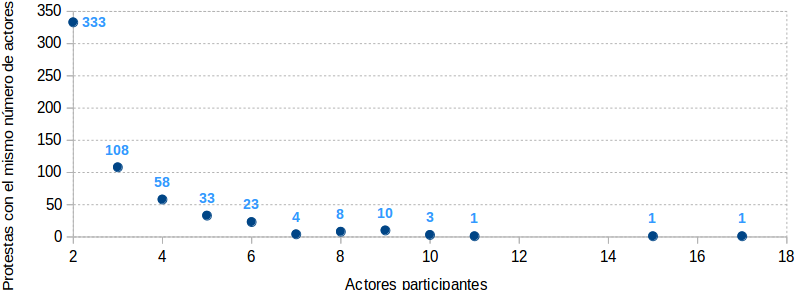
\includegraphics[scale=0.5]{img/3.10_distribucionActores.png}
\par\bigskip
\small Fuente: Elaboración propia.
\end{minipage}\bigskip


Obteniendo la distribución de coparticipaciones en protestas por actor, identificamos en la figura \ref{3.11_participacionesxActor} que, según nuestros datos, más de la mitad (242), registró sólo una protesta en conjunto con otros actores. 
Es decir, que muy pocas organizaciones obtienen una fuerte presencia mediática, mientras que la mayoría es captada episódicamente. 
Por su importancia relativa, indicamos en la tabla  \ref{Actores_con_mayorPresencia} a los 30 actores con mayor número de coaliciones\footnote{
    El resto de los actores (402) tienen 10 o menos coparticipaciones en coaliciones de eventos.
}.




\begin{minipage}{\linewidth}
\centering
\captionof{figure}{Distribución de coparticipaciones en eventos de protesta por actor.} \label{3.11_participacionesxActor}
\hspace{-2em}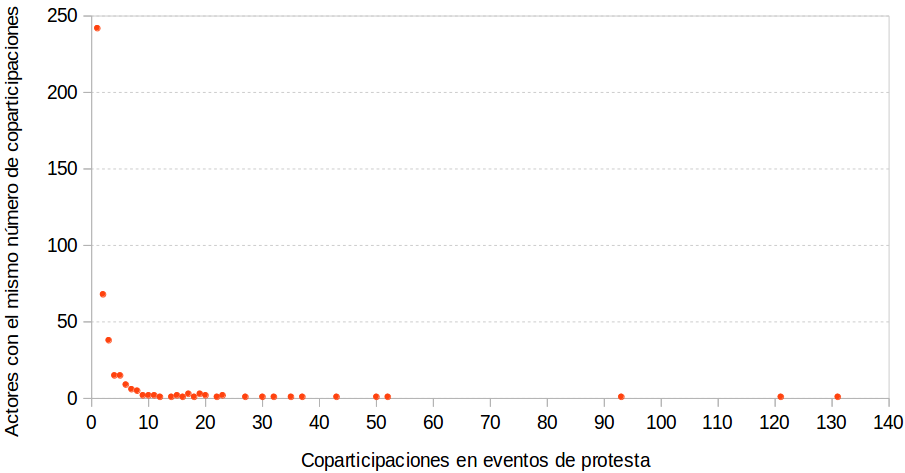
\includegraphics[scale=0.47]{img/3.11_participacionesxActor.png}
\par
\small Fuente: Elaboración propia.
\end{minipage}\bigskip


\begin{table}[!hbt]
\center
\scriptsize
\caption{Actores colectivos con mayor presencia en coaliciones de eventos.}
\label{Actores_con_mayorPresencia}
\begin{tabular}{ | l | c | } 
\hline
\hspace{19em} \textbf{Actor} & \textbf{\# Coaliciones}\\
\hline
Coordinadora Nacional de Trabajadores de la Educación (SNTE - CNTE) -- Sección 7 & 131\\
\hline
Coordinadora Nacional de Trabajadores de la Educación (SNTE - CNTE) -- Sección 40 & 121\\
\hline
Coordinadora Estatal de los Trabajadores de la Educación de Guerrero (CETEG) & 93\\
\hline
Coordinadora Nacional Plan de Ayala - Movimiento de Liberación Nacional (CNPA-MLN) & 52\\
\hline
Coordinadora Nacional de Trabajadores de la Educación (SNTE - CNTE) -- Sección 22 & 50\\
\hline
Coordinadora Nacional de Trabajadores de la Educación (SNTE - CNTE) -- Sección 18 & 43\\
\hline
El Barzón Popular -- Unión Nacional Barzonista & 37\\
\hline
Movimiento Popular Guerrerense (MPG) & 35\\
\hline
Sindicato Mexicano de Electricistas (SME) & 32\\
\hline
Sindicato Único de Servidores Públicos del Estado de Guerrero (SUSPEG) & 30\\
\hline
Coordinadora Nacional de Trabajadores de la Educación (SNTE - CNTE) -- Sección 14 & 27\\
\hline
Federación de Estudiantes Campesinos Socialistas de México (FECSM) & 23\\
\hline
Coordinadora Nacional de Trabajadores de la Educación (SNTE - CNTE) -- Sección 9 & 23\\
\hline
Unión Campesina Democrática (UCD) & 22\\
\hline
Frente Democrático Campesino (FDC) & 20\\
\hline
Coordinadora Nacional de Trabajadores de la Educación (SNTE - CNTE) -- Sin sección identificada & 20\\
\hline
Frente Unido de Normales Públicas del Estado de Guerrero (FUNPEG) & 19\\
\hline
Sindicato de Telefonistas de la República Mexicana (STRM) & 19\\
\hline
Unión Nacional de Trabajadores Agrícolas (UNTA) & 19\\
\hline
Central Independiente de Obreros Agrícolas y Campesinos (CIOAC) & 18\\
\hline
Frente Auténtico del Campo (FAC) & 17\\
\hline
Movimiento Agrario Indígena Zapatista (MAIZ) & 17\\
\hline
Sindicato de Trabajadores de la Universidad Nacional Autónoma de México (STUNAM) & 17\\
\hline
Unión Nacional de Trabajadores (UNT) & 16\\
\hline
Coalición de Organizaciones Democráticas Urbanas y Campesinas (CODUC) & 15\\
\hline
Frente Indígena y Campesino de México (FICAM) & 15\\
\hline
Sindicato Nacional de Trabajadores de la Educación (SNTE) -- Sección 42 & 14\\
\hline
Sindicato Nacional de Trabajadores de la Educación (SNTE) -- Sección 8 & 12\\
\hline
Consejo de Ejidos y Comunidades Opositores a la Presa La Parota (CECOP) & 11\\
\hline
Coordinadora Nacional de Trabajadores de la Educación (SNTE - CNTE) -- Sección 36 & 11\\
\hline
\end{tabular}
\par\bigskip
\caption*{\small Fuente: Elaboración propia.}
\end{table}

\pagebreak



De forma agregada, y considerando ``sectores'' 
(que caracterizan la filiación de los objetivos principales o actividades de cada grupo identificado a uno o dos de los \emph{tipos} idealmente planteados en el \nameref{Anexo_TiposDeActor}) se determinaron 70 categorías, cuya presencia en nuestra base de datos es resumida en la figura \ref{3.12_epsTipos}. 
Las organizaciones \emph{sindicales de maestros} ---disidentes y formales (ED/SPB y SPB/ED respectivamente)--- agrupan la mayor cantidad de actores y coparticipaciones en protestas; otros grupos con fuerte presencia en manifestaciones colaborativas son: \emph{organizaciones campesinas} (CA), \emph{redes plurales} (RP), \emph{sindicatos de trabajadores públicos} (SPB), \emph{estudiantes} (ES) y \emph{productores} (PR).


\begin{minipage}{\linewidth}
\centering
\captionof{figure}{Eventos de protesta y actores (agrupación por sector).} \label{3.12_epsTipos}
\hspace{-2em}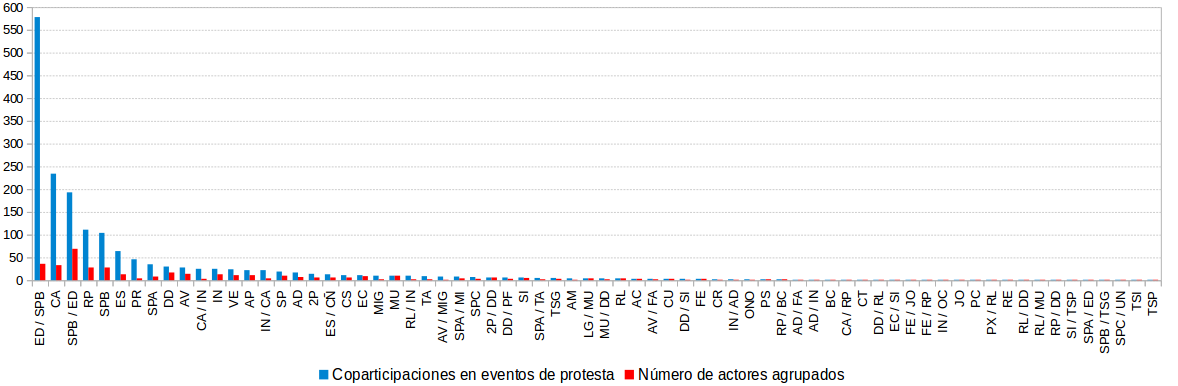
\includegraphics[scale=0.4]{img/3.12_epsTipos.png}
\par\bigskip
\small Fuente: Elaboración propia.
\end{minipage}\bigskip


Se espera que las organizaciones afiliadas al Registro Federal de Organizaciones de la Sociedad Civil (RFOSC) presenten una mayor formalidad y cierta colaboración con el gobierno por la subvención de algunas sus actividades, lo cual explicaría una menor coparticipación en protestas y reclamaciones de orden corporativista cuando ellas tienen lugar (es decir, por la continuidad de recursos y apoyo gubernamental); tal suposición puede ser respaldada por la información agregada que se muestra en la figura \ref{3.13_epsRFOSC}. 
De 52 organizaciones en el RFOSC, el tipo de actor más común registrado es el de \emph{campesinos} (CA) que concentra 20 organizaciones\footnote{
    Se consideran todas las organizaciones registradas en el RFOSC donde el tipo uno o dos es descrito como Campesinos (CA), esto incluye las siguientes combinaciones: CA, CA/IN, CA/RP e IN/CA. Hay 21 organizaciones campesinas más que no están registradas en el RFOSC, que registran 80 coaliciones más.
} 
(3 discretas, 6 matrices y 11 paraguas) quienes en conjunto tienen 202 participaciones en protestas conjuntas. 
Donde buena parte de ellas incluyen demandas donde solicitan recursos y subsidios gubernamentales ---ver figura \ref{4_13_red_tipos_demandas}---, operando como pequeños productores.


\begin{minipage}{\linewidth}
\centering
\captionof{figure}{Eventos de protesta y actores (por su aparición en el RFOSC).} \label{3.13_epsRFOSC}
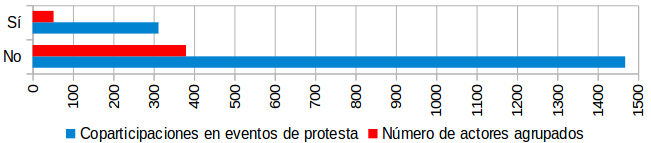
\includegraphics[scale=0.52]{img/3.13_epsRFOSC.png}
\par\bigskip
\small Fuente: Elaboración propia.
\end{minipage}\bigskip

Tomando en consideración el alcance (donde se han documentado actividades) de los actores colectivos identificados, se muestran frecuencias equivalentes en la figura \ref{3.14_epsAlcance}. 
Donde la actividad de las 296 organizaciones locales consignadas es consistente con las frecuencias por ubicación estatal de eventos de protesta, mostradas en la figura \ref{3.5_epsEstados}. 
Por su parte, 119 actores cuya actividad se extiende de forma \emph{nacional} acaparan una mayor coparticipación relativa en nuestra base de datos. 


\begin{minipage}{\linewidth}
\centering
\captionof{figure}{Eventos de protesta y actores (agrupación por alcance de actores).} \label{3.14_epsAlcance}
\hspace{-2em}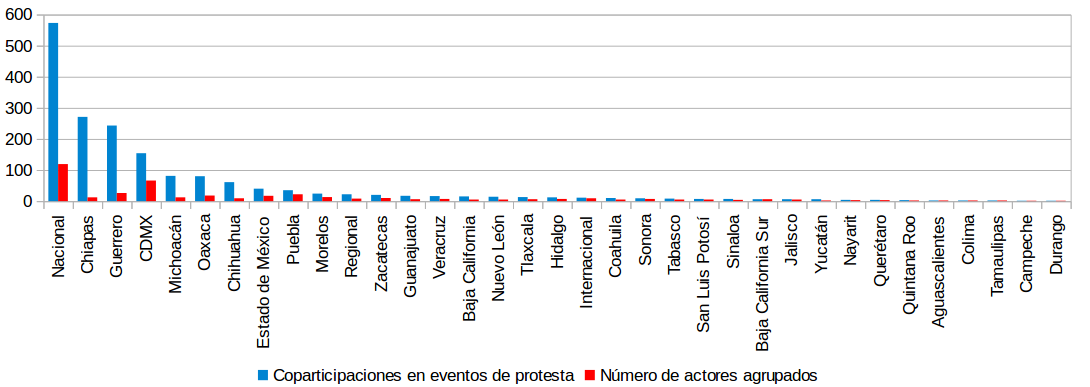
\includegraphics[scale=0.42]{img/3.14_epsAlcance.png}
\par\bigskip
\small Fuente: Elaboración propia.
\end{minipage}\bigskip


En cuanto a las frecuencias por forma organizativa, la figura \ref{3.15_epsFormaOrg} muestra la desproporcionalidad que tienen las organizaciones \emph{económico-gremial} (cuya categoría agrupa a sindicatos, profesionistas y campesinos\footnote{
    En tanto que se consideran productores.
}, 
entre otros actores principales). 
Organizaciones civiles (de lucha por los derechos humanos, contra la violencia, entre otras) no están siquiera cerca de la mitad de las coparticipaciones que registraron los primeros actores.

\begin{minipage}{\linewidth}
\centering
\captionof{figure}{Eventos de protesta y actores (agrupación por forma organizativa).} \label{3.15_epsFormaOrg}
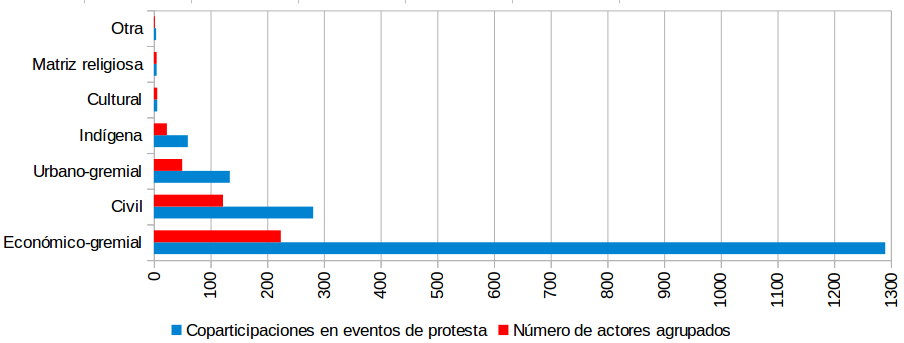
\includegraphics[scale=0.42]{img/3.15_epsFormaOrg.png}
\par\bigskip
\small Fuente: Elaboración propia.
\end{minipage}\bigskip

Finalmente, considerando el tipo de organización, encontramos que las agrupaciones \emph{matrices} (de nuevo, haciendo referencia a sindicatos y agrupaciones usualmente nacionales) tienen una coparticipación mayor, pese a que dicha categoría sólo ocupa el segundo puesto por el número de actores que agrupa.

\begin{minipage}{\linewidth}
\centering
\captionof{figure}{Eventos de protesta y actores (agrupación por tipo de organización).} \label{3.16_epsTipoOrg}
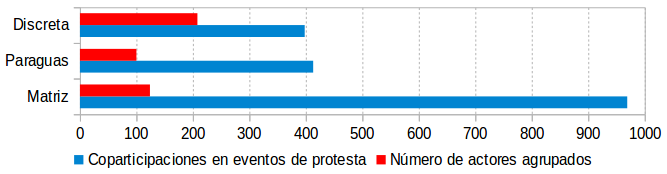
\includegraphics[scale=0.50]{img/3.16_epsTipoOrg.png}
\par\bigskip
\small Fuente: Elaboración propia.
\end{minipage}\bigskip


Creemos que estas diferencias entre actores son relevantes, tanto en términos de su divulgación social (dentro del medio y la consignación realizada), como por el posible impacto relacional en las estructuras analizadas posteriormente (al aprehender principalmente cierto estrato social por las coaliciones muestreadas). 
Al respecto, la asimetría en las frecuencias mostradas puede ser explicada a través de cuatro hipótesis indisociables entre sí: 

\begin{enumerate}
    \setlength\itemsep{0em}
    \item Ya que los actores con mayores participaciones registradas son figuras más claramente identificables; de modo que su continua mención es, hasta cierto punto, sesgada por el reconocimiento (y en ciertos casos, simpatía) que le otorga nuestra fuente periodística. 
    Esto, aunado a la representación asimétrica sobre eventos relacionados (secciones \ref{sec:cobertura} y \ref{sec:EPs largos}) implica sesgos directamente atribuibles a la fracción de la esfera pública que logramos captar.
    
    \item Por otros sesgos, que aunque influenciados por el de la fuente, guardan cierta distancia. 
    En primer lugar, dada la contingencia histórica del periodo analizado, como es posible deducir a partir de las menciones que reciben los temas de la \emph{reforma educativa} y \emph{ayotzinapa} para el periodo muestreado ---ver figuras \ref{3.3_tendenciasTerminos} y \ref{3.17_serieDemandas}---. 
    Y en segundo lugar, ya que los actores con un alcance territorial amplio tienen una presencia más notoria en el país y en particular en las áreas que han recibido una mayor cobertura para las noticias muestreadas ---ver figuras \ref{3.6_epsMunicipios} y \ref{3.14_epsAlcance}---. 
    
    \item Debido a que coaliciones entre un pequeño y cohesivo número de actores es más fácil de llevar a cabo. 
    De modo que la referencia de aquellos actores colectivos que, de forma recurrente protestan en conjunto con otras agrupaciones con las que han formado vínculos estrechos, es consecuentemente más habitual. 
    
    \item Ya que organizaciones gremiales de alcance nacional (fuertemente vinculadas a movimientos sociales, anteriormente adscritos al corporativismo) ejercen una mayor presión que otros grupos, a través de la movilización coparticipativa de sus redes de apoyo. 
    Lo cual es coherente con las observaciones de \citet{2016_Cadena_OMS}, quien refiere una mayor participación general de estos grupos en protestas\footnote{
	Es decir, sin considerar si son coaliciones de eventos o protestas en solitario. 
	Tales observaciones están basadas en datos tomados de las cronologías publicadas por el Observatorio Social de América Latina (OSAL) del Consejo Latinoamericano de Ciencias Sociales (CLACSO) entre 2000 y 2012. 
    }:
	\begin{center}
	    \begin{minipage}{0.9\linewidth}
		{\setlength{\parindent}{12pt}\small
		No podemos dejar de lado que algunas de las organizaciones que tuvieron una presencia más continua en el periodo son organizaciones corporativas que no se caracterizan precisamente por la defensa decidida e íntegra de los intereses de sus miembros, sino que operan como mecanismos de control y de intermediación política. 
		Incluso, algunas de ellas se han convertido en cascarones vacíos. 
		Suponiendo, nuevamente sin conceder, que los datos sean correctos, indican que las OMS que mantienen actividades regulares son la excepción más que la regla, que las OMS más activas son pocas, que son aquéllas que cuentan con estructuras de movilización consolidadas como sindicatos, centrales campesinas o que descansan en estructuras comunitarias estables como las de los pueblos indígenas. 
		Sugieren también que el grueso de las demandas son canalizadas por medios institucionales de carácter corporativo, es decir, que están representadas pobremente. \normalsize \citep[131]{2016_Cadena_OMS}.
		}
	    \end{minipage}
	\end{center}
\end{enumerate}





% BEGIN  DESCRIPCIÓN DE DEMANDAS                                                      
\subsection{Demandas}
\label{sec:demandas}

Las demandas son significativas porque ellas 
permiten ligar múltiples protestas discursivamente, 
pueden ofrecernos algunas pistas sobre los motivos específicos que originan las coaliciones de eventos, 
su filtro mediático puede significar su trascendencia enfatizada ---ante una multitud de discursos---, 
su difusión se extiende al ser presentadas ante más de un actor colectivo (pudiendo trascender a su vez, su vinculación simbólica con un sólo sector particular) 
y podrían reflejar la flexibilidad entre colaboraciones, por la presentación de demandas heterogéneas en un mismo espacio. 


Comenzamos por abordar la relación temporal entre eventos (en \emph{olas}) por las temáticas principales identificadas en nuestros datos; 
posteriormente consideramos la variedad de las \emph{demandas textuales} que se han consignado y por último, presentamos las demandas bajo agrupaciones en \emph{clasificaciones} y su superposición a lo largo de los eventos considerados. 




\subsubsection{Olas de protesta relacionadas con demandas trascendentes}
\label{subsubsec:Olas_demandas}

En la sección \ref{sec:cobertura_temas}, hemos conseguimos identificar dos temas reiterativos, con una amplia \emph{representación mediática} ---estos son: 
(i) la desaparición de los 43 normalistas de \emph{Ayotzinapa} y 
(ii) la \emph{Reforma educativa}, propuesta por el presidente Enrique Peña Nieto---.
Retomamos aquí estas temáticas a fin de establecer una vinculación directa entre estos hechos y las demandas presentadas en los 583 eventos de protesta registrados. 


El aumento y decremento de las protestas donde estas demandas se hacen presentes en el tiempo pueden ser interpretados como \emph{olas de protesta} y, de forma conjunta, como \emph{ciclos de protesta}; es decir, actividades de protesta interrelacionadas, las cuales pueden ser delimitadas en el tiempo ---ver \nameref{AnexoI}---.
En la figura \ref{3.17_serieDemandas} realizamos una agrupación diaria, semanal y mensual, donde podemos suponer la existencia de (al menos) dos ciclos de protesta, uno asociado a cada tema. 
Al respecto, debemos recordar que la tendencia de ciertas coaliciones de eventos puede obtener una mayor representación (respecto al espacio de su divulgación mediática) por dos vías: debido a la cobertura simultánea de varios eventos en un mismo reportaje\footnote{
    Para lo cual resulta útil considerar la agregación diaria de la figura \ref{3.17_serieDemandas}, donde un gran número de eventos en una misma fecha señala la ocurrencia de este fenómeno.
} 
---ver sección \ref{sec:cobertura}--- y por la cobertura sostenida de eventos de protesta de larga duración ---ver sección \ref{sec:EPs largos}---. 



\hspace{-1em}\begin{minipage}{\linewidth}
\centering
\captionof{figure}{Eventos de protesta --- Tendencias asociadas a demandas.} \label{3.17_serieDemandas}
\hspace{-1.5em}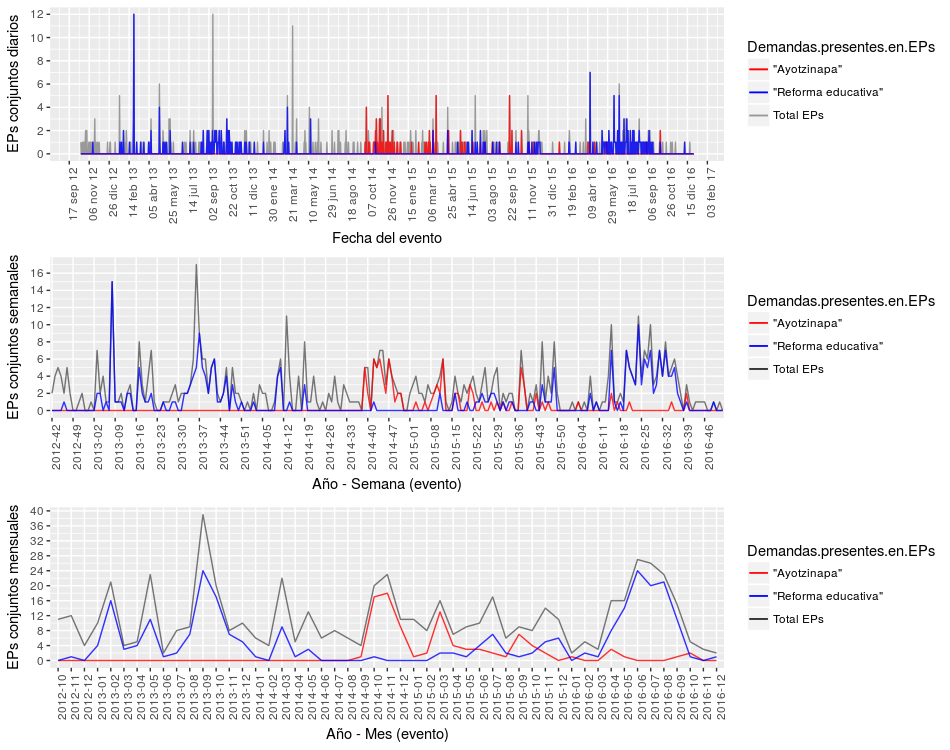
\includegraphics[scale=0.62]{img/3.17_serieDemandas.png}
\par\medskip
\small Fuente: Elaboración propia.
\end{minipage}\medskip



En primer lugar, comprobamos que el tema de la \emph{Reforma educativa} tiene un impacto intermitente (pero extendido en el periodo) dentro de los eventos consignados, donde localizamos 254 protestas en las que se presenta al menos una demanda relacionada. 
Filtrando estas protestas, buscamos periodos de intensa actividad documentada, para lo cual se considera que la diferencia temporal entre una protesta y otra debería ser menor o igual a 10 días\footnote{
    La elección de 10 días es, hasta cierto punto arbitraria, pero consistente con nuestros datos; un valor más alto nos llevaría a aceptar diferencias de 12, 14, 19 días o mayores; con una distancia temporal amplia (similar o mayor a las diferencias nombradas) entre un evento y el siguiente, al inicio o fin de cada ola de protesta.
}. 
De esta forma, existen dos periodos que concentran una mayor cantidad de protestas sobre el tema. 
El primero surge como respuesta ante las leyes secundarias de la reforma educativa, iniciando el 14 de agosto de 2013 y finalizando el 13 de diciembre del mismo año; con una duración propuesta de 121 días, que agrupa 59 eventos de protesta. 
El segundo periodo tiene una duración propuesta de 127 días (del 15 de mayo de 2016 al 19 de septiembre del mismo año), donde se documentan 91 protestas como respuesta a la implementación de la reforma educativa; sin embargo, existe una sobrerrepresentación sobre la cobertura del paro de labores llevado a cabo por las secciones 7 y 40 de la CNTE en Chiapas\footnote{
    Ya que 60 eventos considerados sólo cubren las actividades de esta protesta de larga duración. 
    En realidad, el paro de labores se extendió también a otros estados, pero la mayor parte de la evidencia recolectada (donde se documentó la participación directa de dos o más actores) fue en este caso; por lo tanto (aunque con una relación directa al tema de la reforma educativa y a otros eventos) las referencias en este periodo son más particulares. 
    En el primer periodo, también existió un paro de labores de larga duración y una constante participación de estas secciones; sin embargo, la sobrerrepresentación de actores y lugares de protesta es preeminente en la última ola.
}, de modo que antes que una tendencia general, este último periodo refiere una situación mucho más específica en nuestra submuestra. 


Por otro lado, sólo se contabilizaron 95 eventos de protesta donde se presentan demandas relacionadas con la desaparición de los 43 normalistas de \emph{Ayotzinapa}. 
El único periodo que mantiene una duración sostenida de estas demandas (detectado por el mismo procedimiento, descrito anteriormente) ocurre entre el 29 de septiembre de 2014 y el 27 de diciembre del mismo año, con una duración de 89 días y una agrupación de 45 eventos; donde la mayoría de las protestas se llevan a cabo en el estado de Guerrero, como respuesta inmediata ante la difusión pública del hecho. 


La relación entre estos dos temas ---como anteriormente se había señalado para los reportes periodísticos--- es escasa. 
Sólo 10 protestas plantean demandas entorno a estos hechos de forma simultánea.




\subsubsection{Demandas textuales}
\label{subsubsec:demandas_textuales}

Registramos 1,180 \emph{demandas textuales} en total, distribuidas entorno a las coaliciones de eventos de protesta conforme se muestra en la figura \ref{3.18_demandasxEp}. 

\begin{minipage}{\linewidth}
\centering
\captionof{figure}{Distribución de demandas por evento de protesta.} \label{3.18_demandasxEp}
\hspace{-1em}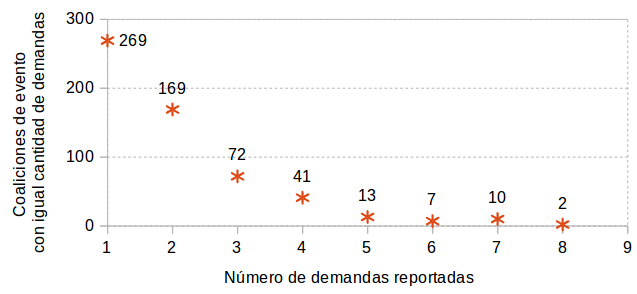
\includegraphics[scale=0.5]{img/3.18_demandasxEp.png}
\par\bigskip
\small Fuente: Elaboración propia.
\end{minipage}\bigskip



Sobresale la demanda ``\emph{[a favor] de la abrogación de la reforma educativa}'', que se replica 84 veces; 
``\emph{[en contra] de la reforma educativa}'', que lo hace 81 veces; 
y ``\emph{[a favor] de la presentación con vida de los 43 normalistas de ayotzinapa desaparecidos}'', con 79 repeticiones. 


El resto de las demandas textuales sólo aparecen 12 o menos veces en las protestas. 
87 demandas textuales\footnote{
    Donde algunas `demandas textuales'' fueron agrupadas siempre que implicaran significados idénticos (expresados en variaciones mínimas de las frases recuperadas), de forma que se han evitado agregaciones más abstractas en este nivel. 
    Se recuerda también que debido al registro de varias protestas, a partir de unos cuantos reportajes, ciertas demandas son replicadas de forma textual entre una protesta y otra. 
} ---como las del párrafo anterior--- permiten la vinculación de 2 o más protestas, mientras que 627 son lo suficientemente específicas como para ser asociadas sólo a una de nuestras 583 protestas conjuntas. 
Esta particularidad nos previene, de nueva cuenta, sobre la tendencia desproporcional en nuestros datos, específicamente ante la continua repetición de las temáticas referidas anteriormente. 


No obstante, al margen de ellas, resulta sobresaliente que varias de las demandas que permiten una vinculación entre eventos en este nivel resultan frases que operan bajo un filtro mediático\footnote{
    O ante una posible falla de atribución o especificación al registrarlas (ya que nuestra depuración ha sido única, y llevada a cabo por quien escribe estas líneas).
}; 
cuya ambigüedad permite equipararlas, pese a que en realidad pueden provenir de diferentes contextos. 
Peticiones por recursos, quejas sobre la violencia, reclamaciones sobre presos políticos o solicitudes de mesas de negociación resultan algunos de los principales temas que permiten encadenar múltiples protestas, lo cual justificamos desde nuestra propia visión de la esfera pública. 
Así, aunque los actores y contextos determinados cambien, a pesar de que no exista una continuidad sobre peticiones específicas, ciertas demandas semejantes (aunque no equivalentes) reflejan preocupaciones básicas sobre expresiones públicas, acentuadas por la fuente, que utilizamos para vincular eventos. 


Tales relaciones son presentadas en la red de la sección \ref{sec:RedGeneral}, como parte de un panorama general, donde la introducción de dichas particularidades facilita el análisis de patrones estructurales agregados. 
Centrarse en cada demanda individual requeriría esfuerzos documentales más exhaustivos; pero ya que nuestra perspectiva en este trabajo es ofrecer una visión del conjunto, presentamos a continuación estas demandas en una forma agregada. 






\subsubsection{Clasificación de demandas}
\label{subsubsec:Clasificacion_demandas}


Las 41 clasificaciones sobre demandas que se consideran aquí son descritas en el \nameref{Anexo_ClasificacionDemandas}, y suponen agregaciones derivadas de las demandas textuales recabadas, como se ha informado en la sección \ref{sec:Esquema_codificacion_LAOMS}. 


\hspace{-1em}\begin{minipage}{\linewidth}
\centering
\captionof{figure}{Frecuencia de demandas por clasificación.} \label{3.19_clasificacionDem}
\hspace{-2em}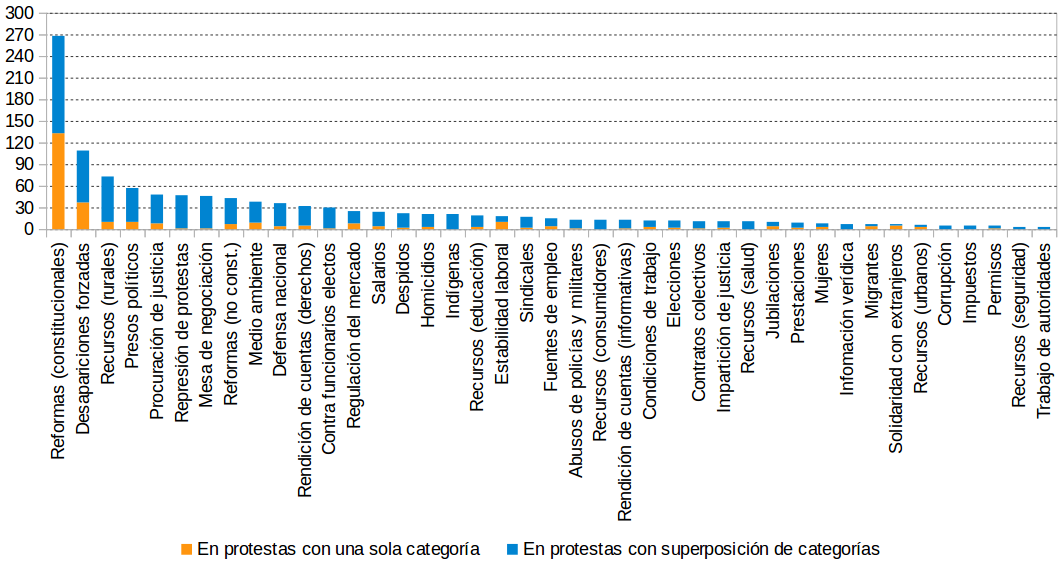
\includegraphics[scale=0.43]{img/3.19_clasificacionDem.png}
\par\bigskip
\small Fuente: Elaboración propia.
\end{minipage}\bigskip


Como se expresó en la figura \ref{3.18_demandasxEp}, en 269 eventos de protesta colaborativos sólo se ha podido identificar una demanda, y (bajo una agregación por clasificaciones de demandas) 12 protestas más incluyen sólo demandas entorno a una misma temática. 
Es importante esta diferenciación, entre protestas \emph{monotemáticas} y otras de carácter más heterogéneo;  
mientras que las primeras informan cuestiones centrales únicas, enfatizadas por la fuente, las segundas ofrecen vínculos temáticos que podrían ser relevantes. 
Es por ello que las frecuencias simples de demandas (donde se realiza esta distinción), son mostradas en la figura \ref{3.19_clasificacionDem}.
Casi la mitad de las protestas (281 coaliciones) son monotemáticas, donde sus demandas resultan congruentes con los principales intereses de los grupos con mayor presencia en nuestros datos (\emph{campesinos} y \emph{maestros sindicalizados}) y con los temas acentuados en la cobertura de nuestra fuente. 


Respecto a las 302 protestas con dos ó más categorías de demandas, resulta interesante saber cuál es el grado de superposición entre nuestras categorías, dada su identificación común en protestas. 
Con este objetivo, y considerado únicamente las 302 protestas referidas, hemos obtenido una matriz donde cada entrada ha sido calculada mediante una generalización del índice de \emph{similaridad de Jaccard}\footnote{
    El índice de Jaccard es uno de los índices binarios de similitud más conocidos y utilizados. 
    Se define como el cociente entre la \emph{cardinalidad de la intersección de dos conjuntos y la cardinalidad de su unión}; es decir, $J(X,Y) = \frac{|X \cap Y|}{|X \cup Y|}$, el cual produce valores acotados entre cero y uno. 
    Su generalización para datos no binarios (también conocida como \emph{similaridad de Ruzicka}) considera dos vectores $\mathbf{x}=(x_{1},x_{2},...,x_{n})$, $\mathbf{y}=(y_{1},y_{2},...,y_{n})$, con $x_{i},y_{i}\geq 0$, donde su similaridad es calculada como: $J(\mathbf{x},\mathbf{y})=\frac{\sum_{i} min(x_{i},y_{i})}{\sum_{i} max(x_{i},y_{i})}$. 
    Consideramos al índice de Jaccard (en su versión binaria o generalizada) como una medida de \emph{superposición relativa} entre dos atributos de las protestas registradas, dada su ocurrencia común. 
    Las intersecciones entre la mayor parte de los atributos en eventos son dispersas y asimétricas, motivo por el que hemos elegido este coeficiente, que toma en cuenta sólo coincidencias efectivas, dada su presencia general. 
    
    Para medir la superposición de demandas en particular, se usa el índice generalizado debido a que más de una demanda reportada en un mismo evento puede ser clasificada en una sola categoría (aunque lo más común es la asociación binaria de clasificaciones en eventos); además, ya que la frecuencia de cada categoría de demandas es de tamaño variable, el índice de Jaccard calculado resulta especialmente afectado en clasificaciones con pocas frecuencias; lo cual debe ser tenido en consideración, dada su asimetría en protestas con superposición de categorías (figura \ref{3.19_clasificacionDem}).
}; 
donde su \emph{intersección} es dada por las protestas donde dos clasificaciones resultan coincidentes, y cuya \emph{unión} es acotada por las protestas donde alguna (o ambas) de estas clasificaciones han sido registradas (según las frecuencias en azul, mostradas en la figura \ref{3.19_clasificacionDem}).


A pesar de que existen pocas superposiciones entre demandas, se registran algunos patrones consistentes con los datos hasta ahora mostrados. 
En primer lugar, sobresalen por su número y grado de superposiciones relativas, las demandas sobre \emph{reformas constitucionales} y \emph{desapariciones forzadas} ---asociadas a nuestras dos temáticas principales (secciones \ref{sec:cobertura_temas} y \ref{subsubsec:Olas_demandas})---; donde la primer clasificación tiene el mayor número de superposiciones con otras demandas, coincidiendo en 32 de las 40 categorías posibles en una o más protestas ---con una relación significativa sobre la instalación de \emph{mesas de negociación} y quejas por la \emph{represión de protestas}---; 
mientras que la segunda, se superpone con 27 categorías y obtiene una mayor similaridad acumulada con ellas ---en especial por su relación con la exigencia de \emph{procuración de justicia} y (en menor medida) en \emph{contra funcionarios electos}---. 


Otras nueve demandas que se superponen con más de la mitad de las categorías posibles en uno o más eventos ---y que, en su mayoría, tienen una frecuencia relativa más grande--- incluyen temáticas que se pueden asociar a agrupaciones gremiales (especialmente a campesinos y empleados sindicalizados), además de las luchas contextuales contra la reforma educativa y las desapariciones forzadas: \emph{represión de protestas}, \emph{presos políticos}, \emph{medio ambiente}, \emph{procuración de justicia}, \emph{salarios}, \emph{reformas no constitucionales}, \emph{mesas de negociación}, \emph{recursos para el campo} y conflictos \emph{sindicales}. 


\begin{minipage}{\linewidth}
\centering
\captionof{figure}{Superposición entre demandas (protestas con más de una categoría).} \label{3.20_simJaccardDem}
  \begin{changemargin}{-1cm}{0cm}
   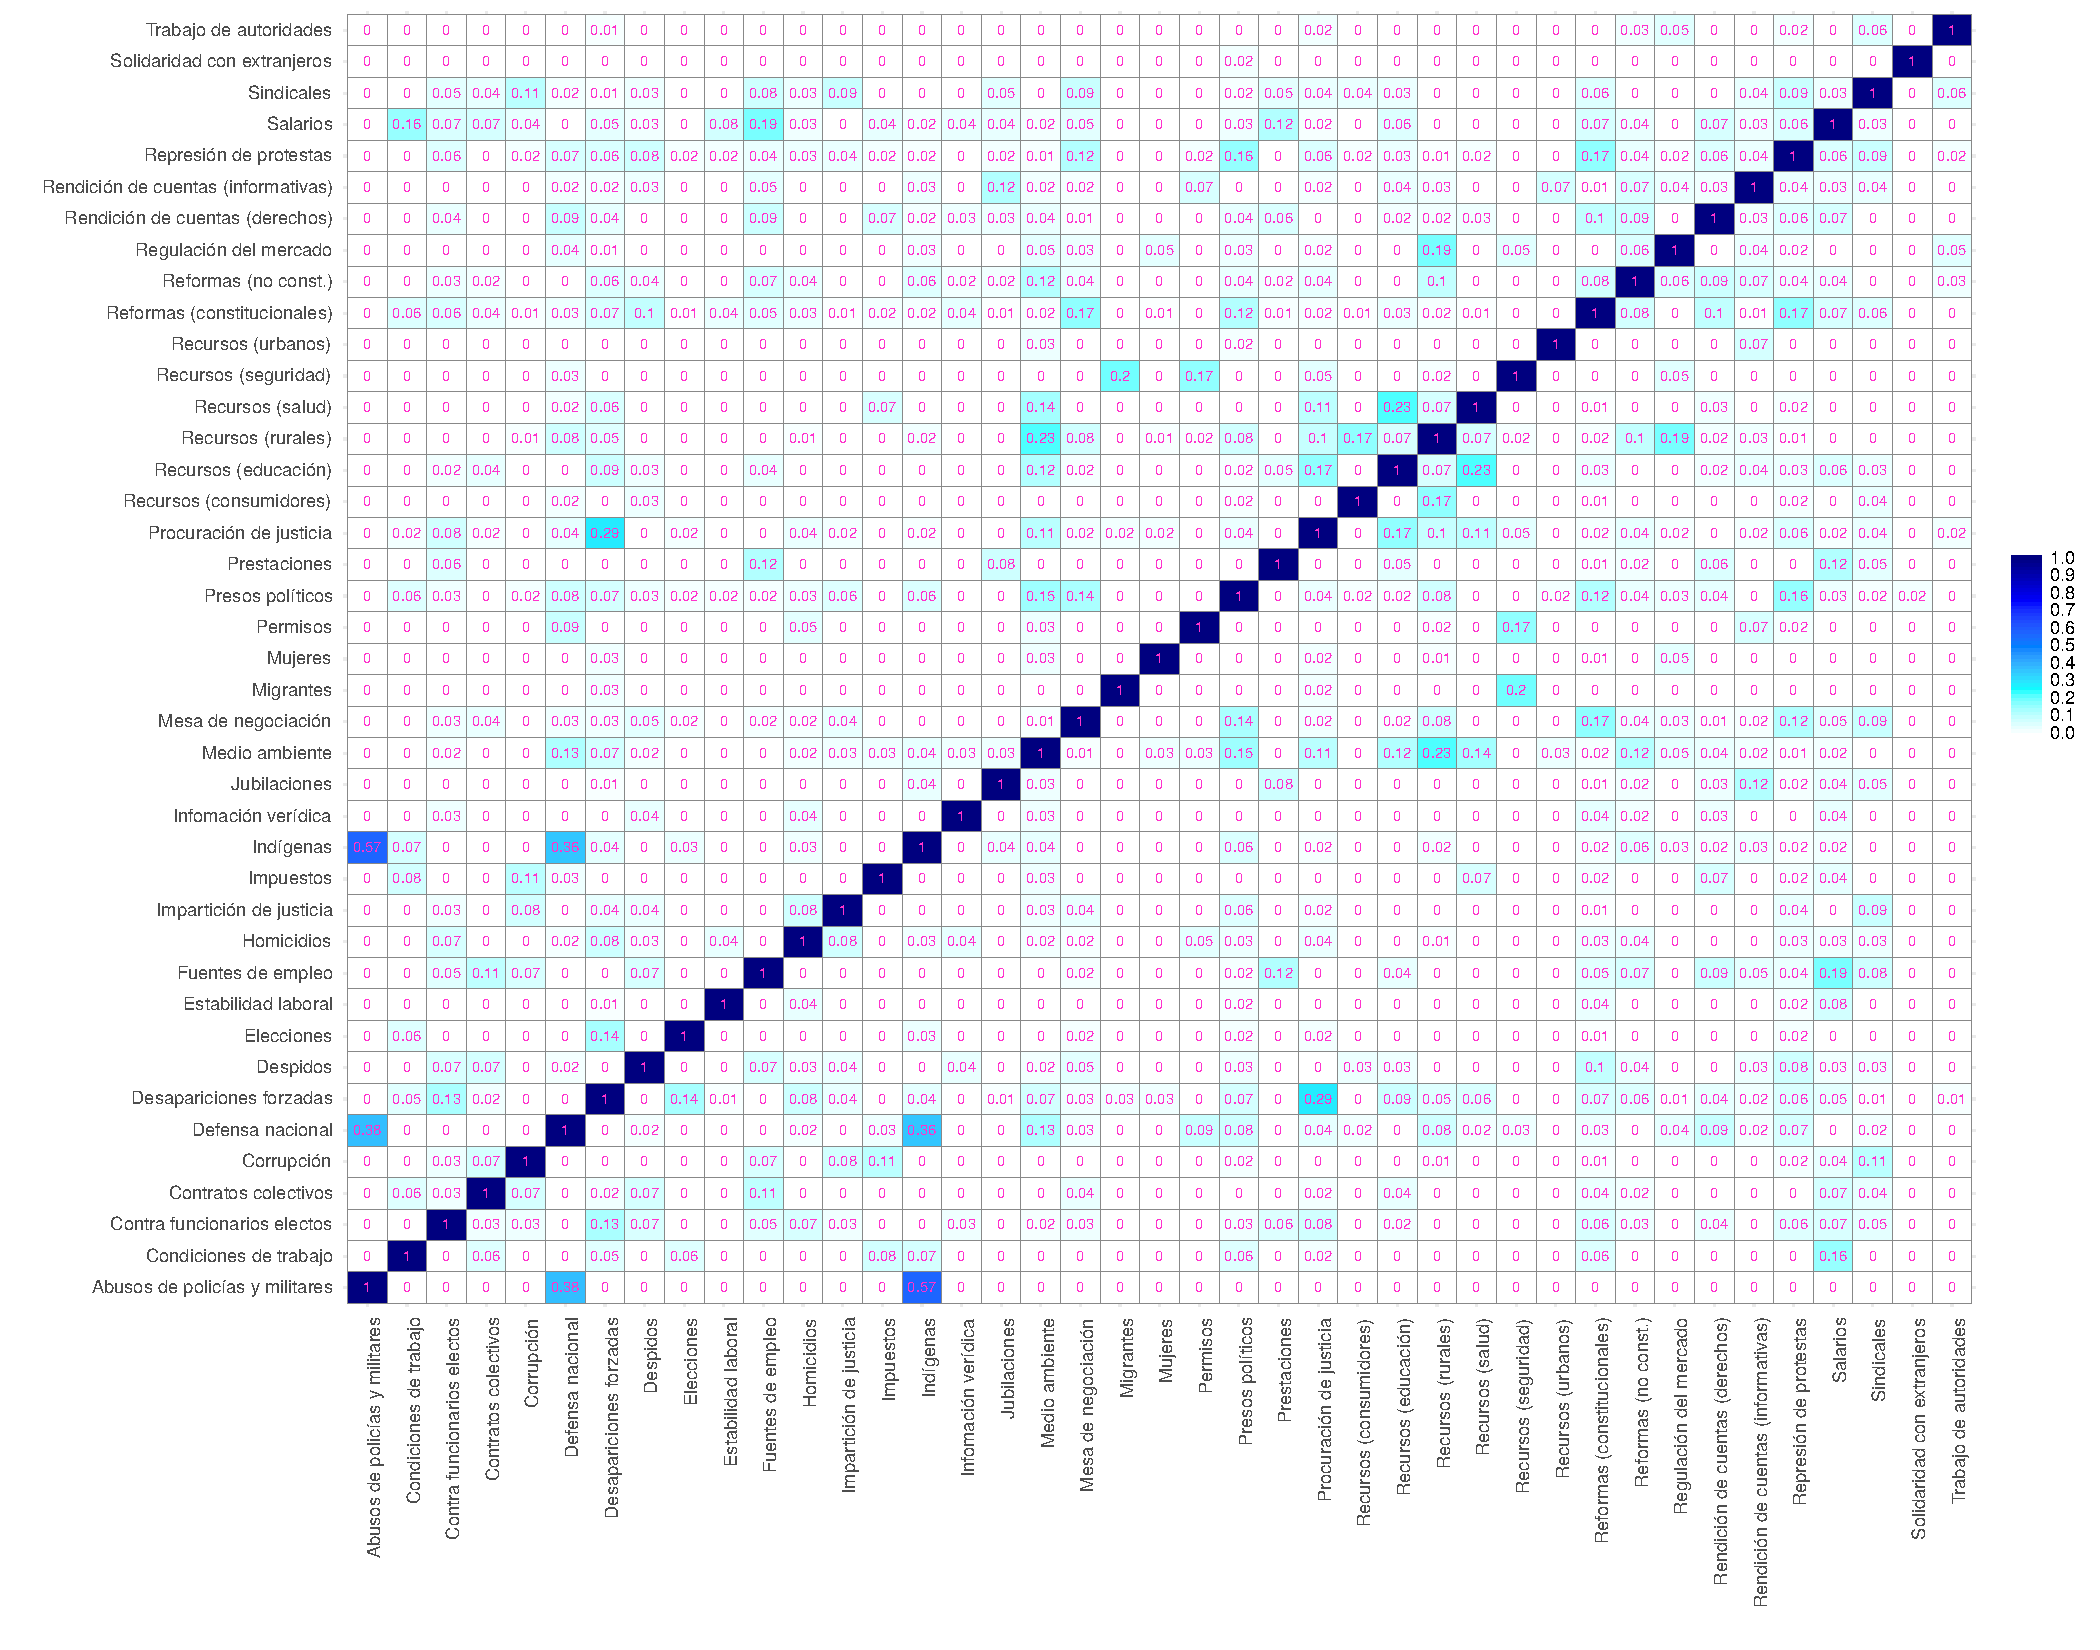
\includegraphics[width=0.8\paperwidth]{img/3_20_simJaccardDem.pdf} 
  \end{changemargin}
\small Fuente: Elaboración propia.
\end{minipage}\bigskip



En el extremo opuesto, comprobamos el aislamiento de las categorías de \emph{solidaridad con extranjeros},  \emph{recursos urbanos},  \emph{migrantes} y \emph{mujeres}; expresadas casi exclusivamente en coaliciones monotemáticas, con seis o menos superposiciones, una baja similaridad agregada, posiblemente vinculadas a un único sector y con poca representación mediática en general (como se observa en la figura \ref{3.19_clasificacionDem}). 


Por último, algunas similaridades atípicas (como la que se establece entre \emph{abusos de policías y militares} e \emph{indígenas}) son derivadas de situaciones contextuales específicas, dada la poca frecuencia que ambas categorías tienen en nuestros datos. 

Si las asociaciones que realizamos son correctas implicaría que, en su mayoría, grupos y temáticas predominantes no sólo son significativas en términos absolutos, por una fuerte resonancia en espacios acotados, sino por su \emph{capacidad para articular múltiples demandas divergentes} a partir de coaliciones de eventos multitemáticas (así implique una intersección absoluta mínima entre ellas). 
A su vez, estos patrones sugieren que múltiples relaciones discursivas no evidentes son llevadas a cabo dentro de coaliciones eventuales reportadas, creando una arena pública contendiente, heterogénea y potencialmente compleja ---como aquella que sugieren \citet{2000_MischePattison_civicArena}---. 
De ahí que resulte especialmente trascendental estudiar sistemáticamente las relaciones entre eventos, actores consignados y las demandas que formulan, lo cual nos ofrecería una pauta más clara sobre coaliciones flexibles y multisectoriales. 
Dichas relaciones (directas y proyectadas) son analizadas en el siguiente capítulo.  






% BEGIN  DESCRIPCIÓN DE REPERTORIOS                                                      
\vspace{-1em}
\subsection{Repertorios de protesta}
\label{sec:repertorios}

Una distinción entre protestas \emph{pacíficas} y \emph{violentas} ha sido establecida, basada en los actos de protesta empleados por los manifestantes en cada evento, de acuerdo al \nameref{Anexo_RepertoriosPacificos} y \nameref{Anexo_RepertoriosViolentos}. 
De 583 protestas colaborativas, 534 fueron catalogadas como pacíficas, ---donde suponemos que el tipo de menciones (u omisiones) que son originadas desde la fuente periodística juegan un papel fundamental---; sólo una fue encontrada violenta\footnote{
    Donde la consignación de este evento es derivada de una mención breve (junto al reporte de otros eventos de temáticas similares) en el contexto de protestas de la CNTE en Oaxaca, durante enero de 2015. 
}; 
y 48 protestas más involucran tanto repertorios pacíficos como violentos. 


\hspace{-1em}\begin{minipage}{\linewidth}
\centering
\captionof{figure}{Frecuencia de repertorios de protesta.} \label{3.21_repertorios}
\hspace{-1em}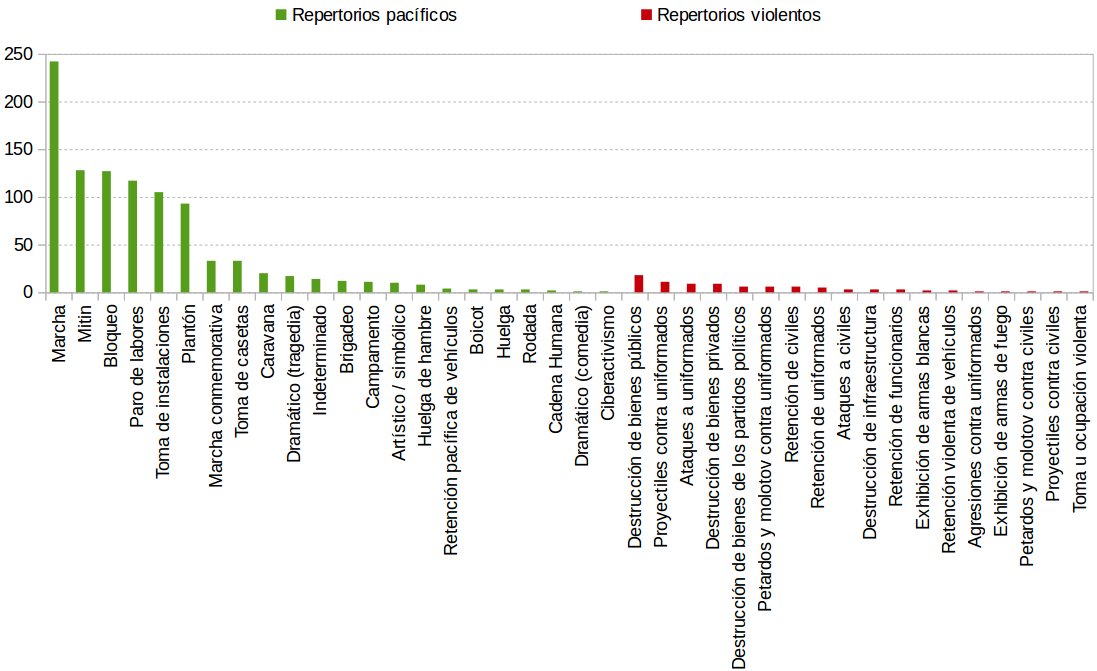
\includegraphics[scale=0.36]{img/3.21_repertorios.png}
\par
\small Fuente: Elaboración propia.
\end{minipage}\bigskip


Por su frecuencia simple (mostrada en la figura \ref{3.21_repertorios}), se observa la poca presencia absoluta que los repertorios violentos tienen en nuestros datos, tratándose de forma colateral y estando acompañados en 27 casos de la intervención de las fuerzas del orden público. 
De estos 27 eventos, que involucran enfrentamientos directos entre manifestantes y policías o granaderos, la fuente sugiere intentos de contención (por ejemplo, desalojos o cercos policiales) que desencadenan en actos violentos; o (en menor medida) acciones radicales promovidas por algunos manifestantes como recurso de negociación o expresión de hartazgo\footnote{
    Como comparación, otras 38 intervenciones de la fuerza pública fueron detectadas durante protestas pacíficas, en contraposición con 496 eventos pacíficos, que no tuvieron ninguna intervención reportada. 
    Estas y otras respuestas derivadas de un evento son discutidas en la sección \ref{sec:respuestaProtesta}. 
}. 
 

Bajo una perspectiva de colaboración entre dos o más actores colectivos, tiene sentido suponer que los repertorios violentos implican una medida desesperada por captar la atención sobre las demandas formuladas y sólo son empleados en situaciones límite o por coaliciones entre grupos informales, que no se ocupan demasiado de su imagen pública. 




275 protestas emplearon sólo un repertorio, mientras que 800 repertorios más (de los que son mostrados en la figura \ref{3.21_repertorios}) son distribuidos en los 308 eventos restantes, conforme se indica en la tabla \ref{Distribucion_repertorios_Eps}. 
La combinación de ciertos repertorios pacíficos y violentos (dada la relativa intersección en marchas conmemorativas, mítines y retenciones de vehículos) manifiesta que la frontera que separa actos agresivos de aquellos que no lo son, no siempre es evidente; de allí que la intencionalidad en algunas protestas podría ser más contenciosa que la que se sugiere en la fuente. 
En otras combinaciones existe una baja consistencia en la ejecución de acciones razonablemente emparentadas, lo cual podría reflejar (como hemos sugerido anteriormente) el surgimiento contingente de conflictos en protestas, con intencionalidad inicial pacífica ---o representada de tal forma--- y cuyos participantes reaccionan de forma violenta ---o se les justifica así--- a represiones o contenciones ejercidas por las fuerzas del orden. 


\begin{table}
\center
\scriptsize
\caption{Distribución de repertorios de protesta por protesta.}
\label{Distribucion_repertorios_Eps}
\begin{tabular}{ | C{8em} | C{9em} | C{9em} | C{9em} | }
\hline
\textbf{Cantidad de repertorios empleados} & \textbf{Protestas pacíficas} & \textbf{Protestas pacíficas y violentas} & \textbf{Protestas violentas} \\
\hline
{\small \textbf{1} }& 275 & 0 & 0\\
\hline
{\small \textbf{2} }& 183 &  13 & 1 \\
\hline
{\small \textbf{3} }& 55 &  10 & 0 \\
\hline
{\small \textbf{4} }& 18 &  11 & 0 \\
\hline
{\small \textbf{5} }& 3 &  9 & 0 \\
\hline
{\small \textbf{6} }& 0 &  2 & 0 \\
\hline
{\small \textbf{7} }& 0 &  2 & 0 \\
\hline
{\small \textbf{9} }& 0 &  1 & 0 \\
\hline
\end{tabular}
\par\bigskip
\caption*{\small Fuente: Elaboración propia.}
\end{table}


Obteniendo la matriz de superposiciones entre repertorios (por el índice binario de similaridad de Jaccard, en la figura \ref{3.22_simRepertorios}), encontramos que los repertorios con menor representación en nuestros datos frecuentemente se acompañan de repertorios más comunes (\emph{marchas}, \emph{mítines} y \emph{bloqueos}). 
Otros repertorios con importantes frecuencias: \emph{plantones}, \emph{paros de labores} y \emph{toma de instalaciones} (ocasionalmente vinculados a eventos de protesta de larga duración ---ver sección \ref{sec:EPs largos}---); también tienen un número de superposiciones significativas, a pesar de que los índices calculados no sean demasiado grandes (dada la asimetría de las comparaciones). 
Finalmente, la tendencia más evidente relaciona fuertemente a gran parte de los repertorios violentos entre sí, dada su pequeña frecuencia, concentrada alrededor de unos pocos eventos. 


Los repertorios de protesta utilizados ``pueden dar cuenta del grado de organización o planeación que ostenta un contingente o cúmulo de participantes'' \citep[27]{2017_Urbina_estudiantes}; donde el número mínimo de manifestantes requeridos, la elección de repertorios empleados (dados los objetivos enfrentados) y cierta coordinación de actividades puede ser clave para el éxito de una protesta colaborativa ---como hemos mencionado en la sección \ref{subsubsec:CoalicionesEventos}---. 
En ese sentido, y tomando en consideración a los repertorios más utilizados, su predominancia y correlación con repertorios menos comunes, la conjunción de tales acciones de protesta corrientes (que requieren distintos grados de organización) puede plantear \emph{coaliciones heterogéneas}, con distintos tipos de sistematización en el periodo y una baja capacidad de innovación ---si bien, vale la pena recordar que nuestro muestreo de noticias podría favorecer repertorios más comunes---. 
Al margen de tales acciones, hay repertorios de distinto orden: más novedosos, contingentes y episódicos, que tienen poca presencia general en nuestra muestra. 

Por otra parte, las frecuencias desproporcionales observadas pueden ser explicadas por el sesgo geográfico operado (como se ha sugerido en la figura \ref{3.8_epsGeolocalizacion}). 
Marchas, mítines, paros de labores y tomas de instalaciones pueden ser asociados en su mayoría a áreas urbanas (por las oportunidades que ofrecen dichas demarcaciones); 
mientras que bloqueos, caravanas y tomas de casetas son repertorios estratégicos empleados en puntos carreteros clave, que pueden involucrar menor cobertura. 

\begin{minipage}{\linewidth}
\centering
\captionof{figure}{Superposición entre repertorios de protesta.} \label{3.22_simRepertorios}
\hspace{-4em}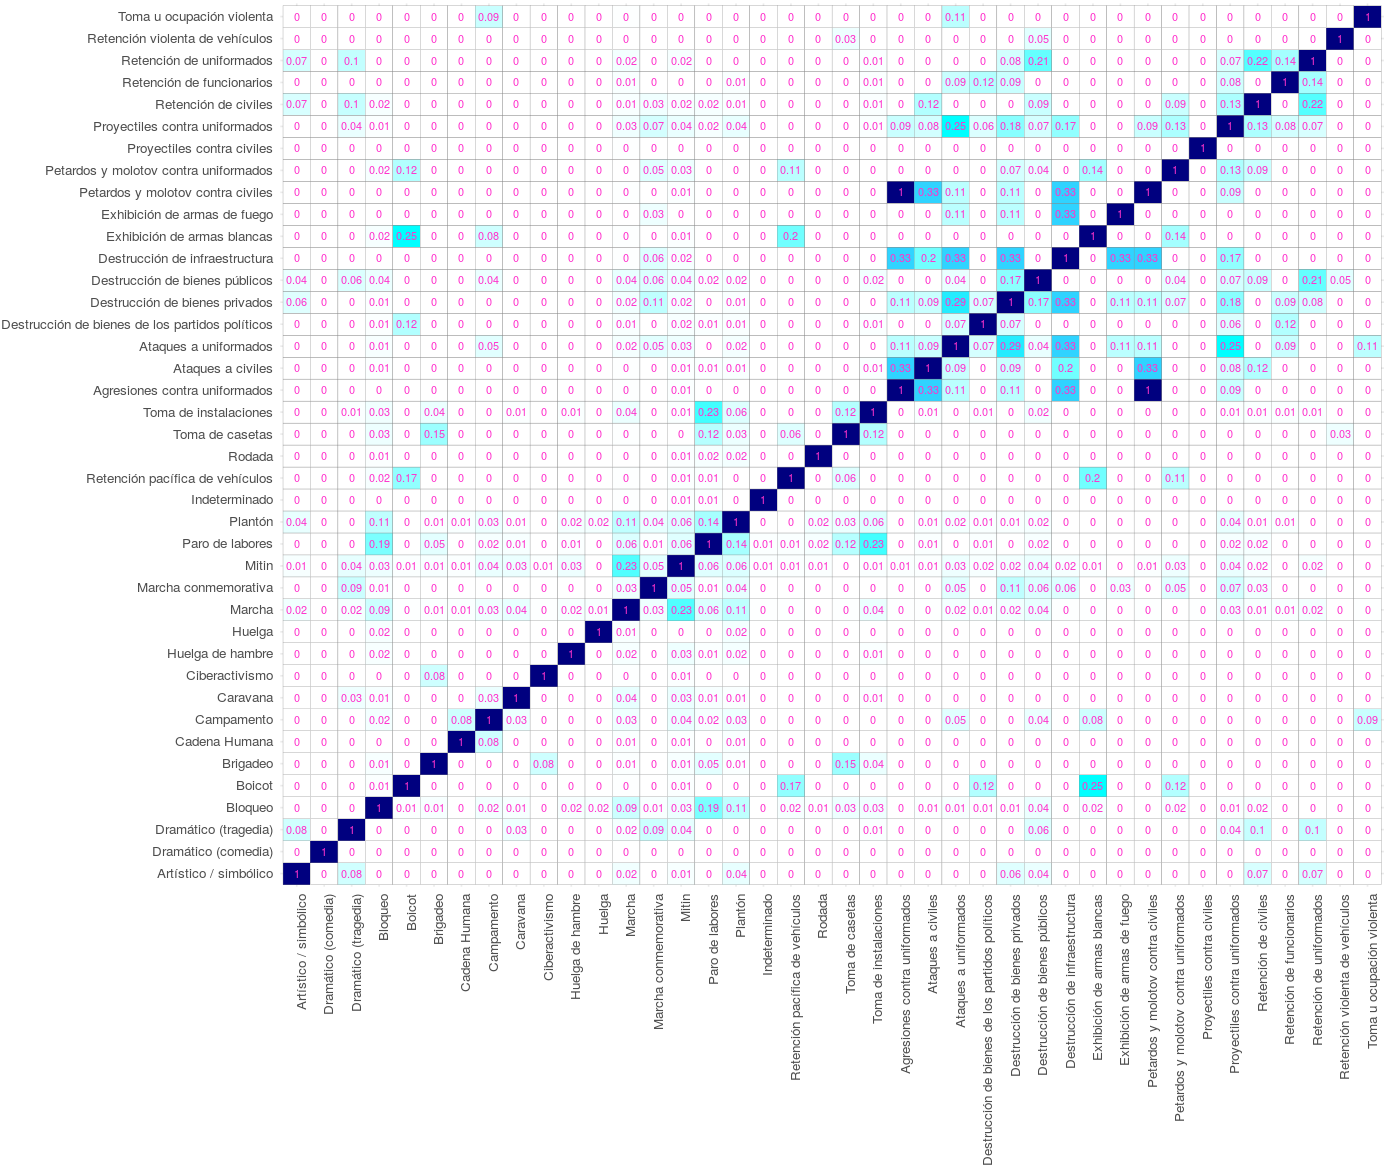
\includegraphics[scale=0.44]{img/3.22_simRepertorios.png}
\par
\small Fuente: Elaboración propia.
\end{minipage}\bigskip


Para finalizar nuestra descripción sobre repertorios, recuperamos la discusión de la sección \ref{sec:NotiMuestreo}, sobre los diferentes muestreos involucrados en nuestra base de datos. 
Nuestra hipótesis ---recuperada del trabajo de \citet{2010_Strawn_keywordSearch}, \citet{2001_Maney_Oliver__FindingEvents}--- sugiere que durante el primer protocolo (basado en \emph{búsquedas textuales}), la recuperación de noticias pudo ser afectada por una preferencia hacia la diferenciación central de contenido; y que durante la aplicación del segundo periodo de muestreo (basado en \emph{palabras clave}), se diera preferencia a acciones comunes de protesta. 

Si nuestra hipótesis es correcta, esperaríamos hallar una diferencia clara sobre los repertorios en cada periodo. 
Para aproximar tal afectación real, diferenciamos (por las fechas de nuestras fuentes) las protestas muestreadas entre un protocolo y otro. 
Los resultados de este conteo (mostrados en la tabla \ref{Muestreo_repertorios}) son sugerentes, pues reflejan algunas discrepancias de tendencias relativas; pero no resultan concluyentes debido a la irregularidad temporal en: (i) protestas (sección \ref{subsubsec:DimensionTemporal}) y (ii) aplicación de protocolos (3 meses de búsquedas textuales ---relacionados a 56 protestas--- y 48 meses utilizando palabras clave ---derivando en 527 eventos---). 


\begin{table}[H]
\scriptsize
\centering
\captionof{table}{Comparación de repertorios muestreados bajo distintos protocolos.} \label{Muestreo_repertorios}
\begin{tabular}{ | l | c | c | }
\cline{2-3}
\multicolumn{1}{c|}{ } & \textbf{Búsqueda textual} & \textbf{Palabras clave} \\
\hline
Artístico / simbólico & 0 & 10\\
\hline
Dramático (comedia) & 0 & 1\\
\hline
Dramático (tragedia) & 0 & 17\\
\hline
Bloqueo & 11 & 116\\
\hline
Boicot & 0 & 3\\
\hline
Brigadeo & 1 & 11\\
\hline
Cadena Humana & 0 & 2\\
\hline
Campamento & 3 & 8\\
\hline
Caravana & 2 & 18\\
\hline
Ciberactivismo & 0 & 1\\
\hline
Huelga de hambre & 1 & 7\\
\hline
Huelga & 2 & 1\\
\hline
Marcha & 24 & 218\\
\hline
Marcha conmemorativa & 0 & 33\\
\hline
Mitin & 10 & 118\\
\hline
Paro de labores & 11 & 106\\
\hline
Plantón & 10 & 83\\
\hline
Indeterminado & 0 & 14\\
\hline
Retención pacífica de vehículos & 0 & 4\\
\hline
Rodada & 1 & 2\\
\hline
Toma de casetas & 7 & 26\\
\hline
Toma de instalaciones & 22 & 83\\
\hline
Agresiones contra uniformados & 0 & 1\\
\hline
Ataques a civiles & 0 & 3\\
\hline
Ataques a uniformados & 0 & 9\\
\hline
Destrucción de bienes de los partidos políticos & 0 & 6\\
\hline
Destrucción de bienes privados & 0 & 9\\
\hline
Destrucción de bienes públicos & 0 & 18\\
\hline
Destrucción de infraestructura & 0 & 3\\
\hline
Exhibición de armas blancas & 0 & 2\\
\hline
Exhibición de armas de fuego & 0 & 1\\
\hline
Petardos y molotov contra civiles & 0 & 1\\
\hline
Petardos y molotov contra uniformados & 0 & 6\\
\hline
Proyectiles contra civiles & 0 & 1\\
\hline
Proyectiles contra uniformados & 0 & 11\\
\hline
Retención de civiles & 0 & 6\\
\hline
Retención de funcionarios & 0 & 3\\
\hline
Retención de uniformados & 0 & 5\\
\hline
Retención violenta de vehículos & 0 & 2\\
\hline
Toma u ocupación violenta & 0 & 1\\
\hline
\textbf{Total} & \textbf{105} & \textbf{970} \\
\hline
\end{tabular}
\par\bigskip
\caption*{\small Fuente: Elaboración propia.}
\end{table}





% BEGIN  DESCRIPCIÓN DE OBJETIVOS                                                      
\subsection{Objetivos}
\label{sec:Opositores}


Este campo está dirigido al registro de organizaciones e instituciones a las que los protestantes dirigen sus demandas  y pretende responder a la pregunta de investigación ¿ante quién se protesta? ---según \citet{2017_Cadena_ManualLAOMS}---. 


Al respecto, suponemos tres sesgos, cuyo origen es distintivo: 
(i) por nuestra \emph{fuente periodística} (como se sugiere en  la figura \ref{2.4_sesgo_oficial_vs_medios}) y en nuestro caso particular bajo la suposición que \emph{La Jornada}, al constituirse como un diario de oposición, puede ser impulsado a identificar más reiterativamente objetivos políticos importantes;  
(ii) por la \emph{cobertura geográfica}, ya que nuestros datos se centran en algunas de las principales ciudades de los estados (como se muestra en la figura \ref{3.6_epsMunicipios}), particularmente en la Ciudad de México, donde existe una mayor cantidad de dependencias federales; 
y (iii) por \emph{decisiones metodológicas}, dado el criterio para identificar objetivos en función del lugar elegido para protestar. 


Las frecuencias mostradas en la tabla \ref{Opositores} siguen estas orientaciones; haciendo resaltar especialmente que, en nuestros datos, protestas colaborativas identifican como objetivos más comunes aquellos dentro del sector público y de ámbito federal. 
Específicamente, más de la mitad de las protestas con objetivos identificados se centran en dependencias relacionadas por el poder ejecutivo federal, el cual engloba distintas secretarías. 


\begin{table}[H]
\scriptsize
\centering
\captionof{table}{Objetivos identificados por función y sector.} \label{Opositores}
\begin{tabular}{ | m{16em} | C{3.7em} | C{3.4em} | C{4.9em} | C{6.3em} | C{3.3em} | C{2.5em} | }
\cline{2-7}
\multicolumn{1}{c|}{ } & \multicolumn{6}{c|}{ \textbf{Sector}  }\\
\hline
\textbf{Función} & \textbf{Público (federal)} & \textbf{Público (estatal)} & \textbf{Público (municipal)} & \textbf{Público (internacional)} & \textbf{Privado} & \textbf{Social}\\
\hline
Agrupación de trabajadores &  &  &  &  &  & 3\\
\hline
Asamblea ejidal &  &  &  &  &  & 1\\
\hline
Autónomo / garante & 14 & 1 &  &  &  & \\
\hline
Comercio (al por mayor y al por menor) &  &  &  &  & 3 & \\
\hline
Ejecutivo & 276 & 102 & 15 &  &  & \\
\hline
Embajada &  &  &  & 2 &  & \\
\hline
Gobierno extranjero &  &  &  & 2 &  & \\
\hline
Judicial & 7 & 8 &  &  &  & \\
\hline
Legislativo & 25 & 39 &  &  &  & \\
\hline
Medios de comunicación &  &  &  &  & 9 & \\
\hline
Minería y extracción de petróleo &  &  &  &  & 6 & \\
\hline
No identificado & 11 & 3 &  &  &  & \\
\hline
Organización internacional &  &  &  & 2 &  & \\
\hline
Partidos políticos & 6 & 2 &  &  &  & \\
\hline
Población en general &  &  &  &  &  & 1\\
\hline
Transportes y comunicaciones &  &  &  &  & 2 & \\
\hline
\textbf{Total} & \textbf{339} & \textbf{155} & \textbf{15} & \textbf{6} & \textbf{20} & \textbf{5}\\
\hline
\end{tabular}
\par\bigskip
\caption*{\small Fuente: Elaboración propia.}
\end{table}

Las iniciativas de reformas estructurales, los actos de corrupción que se le imputaron desde los medios y la poca popularidad de la que ha gozado el presidente de la república, le hacen el objetivo más recurrente (en 64 eventos). 
Dentro de este mismo sector, le siguen la secretaría de gobernación y la secretaría de educación pública (en 50 y 48 eventos, respectivamente); las cuales son vinculadas a la reforma educativa y la desaparición de los 43 estudiantes de Ayotzinapa; sobresale que al no obtener acuerdos a nivel federal, los congresos estatales y las secretarías de educación pública estatales fueron el objetivo (en 33 y 26 casos respectivamente) de opositores a las reformas estructurales. 
Los gobiernos estatales también son objetivos importantes (identificados en 62 protestas) en comparación con las presidencias municipales (que sólo son increpadas directamente en 13 eventos). 
Algunas dependencias que liberan fondos para sectores agrarios corporativistas\footnote{
    Como la Secretaría de Agricultura, Ganadería, Desarrollo Rural, Pesca y Alimentación (SAGARPA); la Comisión Nacional para el Desarrollo de los Pueblos Indígenas (CDI); la Secretaría de Desarrollo Agrario, Territorial y Urbano (SEDATU); y la Secretaría de Desarrollo Social (SEDESOL). 
} 
son objetivos más específicos que sólo aparecen una decena de veces o menos. 
Finalmente, otros objetivos identificados obedecen a situaciones contextuales más específicas, por lo que su aparición es periférica e incidental. 


Respecto a la distribución de estos objetivos: en 181 eventos colaborativos no se detectó ningún objetivo; 284 protestas refieren un único objetivo; 96 eventos más indican 2 objetivos y sólo 22 protestas alcanzan el límite de consignación de tres objetivos. 


Esta información insinúa que las coaliciones captadas en nuestros datos son formadas como frentes comunes, con objetivos políticos relevantes en el país y en ciertos estados con alta representatividad; donde su importancia emblemática y la capacidad resolutiva de tales objetivos hace que el flujo de manifestaciones se canalicen hacia ellos. 




% BEGIN  DESCRIPCIÓN DE RESPUESTAS                                                      
\subsection{Respuestas a la protesta}
\label{sec:respuestaProtesta}


Las respuestas a las protestas colaborativas corresponden a interacciones comprobadas con figuras de autoridad (principalmente funcionarios públicos y fuerzas del orden público) registradas por nuestra fuente y consignadas en atributos binarios para cada una de las 583 coaliciones consideradas. 
Únicamente 133 de estos eventos registraron una o más respuestas, las cuales son mostradas por su frecuencia en la figura \ref{3.23_respuestas}. 
Como en otras características registradas, para que una respuesta sea reflejada en nuestros datos se deben cumplir varias condiciones: 
(i) que tal respuesta sea generada en el transcurso del evento (de forma pública) de modo que se pueda captar su ocurrencia y resultado; 
(ii) que el reportero recabe información sobre tales interacciones; 
(iii) que la publicación en nuestra fuente resulte en una crónica consecuente; 
(iv) que se consiga muestrear tal contenido periodístico ---recuperado en nuestra submuestra por tratarse además de un acto coparticipativo---; 
y (iv) que no existan omisiones de captura. 

\hspace{-1em}\begin{minipage}{\linewidth}
\centering
\captionof{figure}{Respuestas ante la protesta.} \label{3.23_respuestas}
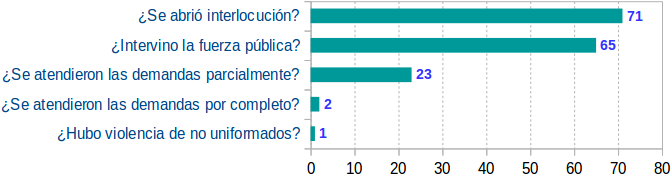
\includegraphics[scale=0.55]{img/3.23_respuestas.png}
\par\bigskip
\small Fuente: Elaboración propia.
\end{minipage}\bigskip

De forma general, estos \emph{procesos de gestión} contemplan tres grandes rubros ---descritos por \citet{2017_Rob_Respuestas}---: 
(i) \emph{atención a las demandas} ---parcial (solamente algunas) o completa (todas ellas)---; 
(ii) \emph{interlocución}; 
e (iii) \emph{intervención de la fuerza pública} ---que considera el despliegue de policías y demás cuerpos del orden público para contener, desarticular o interrumpir una protesta---.
Donde la violencia de no uniformados resulta en un único caso aislado, que usualmente no es considerado en conteos generales\footnote{
    Aunque este caso no se resulte orientativo sobre tendencias generales en nuestros datos, este caso es emblemático por su relevancia en la identificación (poco común) de policías vestidos de civil; durante la marcha de 2013 en la Ciudad de México conmemorativa del 2 de octubre. Fuente: \url{http://www.jornada.unam.mx/2013/10/03/politica/003n2pol}.
}. 


Según las frecuencias de la figura \ref{3.23_respuestas}, en protestas colaborativas ---dadas nuestras condiciones previas--- la respuesta más común es la interlocución con manifestantes (que aglomera el 43.83\% de las respuestas registradas), seguida de la intervención de la fuerza pública (con el 40.12\% de respuestas) y la menos común es la atención de demandas (que considera sólo un 15.43\% de las protestas con respuestas)\footnote{
    Es importante observar que estos porcentajes relativos son diferentes en la base de datos general del LAOMS (específicamente, en protestas con respuestas registradas entre el 1 de diciembre de 2012 y el 31 de diciembre de 2016), cuyos valores reportados son del 38.13\%, 30.40\% y 31.48\% respectivamente. 
    Como en las coaliciones de eventos que depuramos para esta tesis, se realizó un trabajo análogo para la submuestra de 1,547 protestas con respuestas registradas, por parte de  \citet{2017_Rob_Respuestas} para obtener estos porcentajes, con especial énfasis en estos rubros. 
    Estas discrepancias pueden representar diferencias por las características específicas de respuestas colaborativas o debido a diferentes omisiones en la consignación original de los datos. 
}


La atención e interlocución es lo que se esperaría en un régimen democrático que respetase el derecho a la protesta ---usualmente amparado en el derecho de reunión\footnote{
    Aunque esto excluiría formas ilegales de protesta, como el boicot, ciertas huelgas y actos violentos. 
}---, mientras que la intervención de la fuerza pública puede ser vista como la cara represiva del gobierno\footnote{
    Donde sus responsabilidades sobre mantener cierto orden público y la seguridad de manifestantes y público en general a menudo resultan contradictorias y discrecionales. 
}, pese a que estas dicotomías frecuentemente sean rebasadas ---observación que también hace \citet{2017_Rob_Respuestas}---. 
Al respecto, distintas organizaciones y activistas han puesto énfasis en que:
\begin{center}
    \begin{minipage}{0.9\linewidth}
        {\setlength{\parindent}{12pt}\small
	    (...) la evidencia muestra una tendencia preocupante hacia el impedimento y represión de la protesta social. 
	    Dicha tendencia se manifiesta principalmente por un marcado rechazo a las expresiones sociales de denuncia y exigencia, por el impulso de disposiciones normativas que expresamente buscan regularlas, por la imposición de medidas de restricción y sanción al ejercicio ciudadano de derechos, así como por la criminalización de quienes participan en ellas. \normalsize \citep[7]{2015_LibertadExpresion_Represion}.
        }
    \end{minipage}
\end{center}

De las 65 protestas donde se registraron intervenciones de la fuerza pública (figura \ref{3.23_respuestas}), hubo 39 bloqueos, 9 encapsulamientos, 10 desalojos y 35 agresiones por parte de uniformados. 
Estas últimas agresiones son diferenciadas en: (i) \emph{agresiones proporcionales} (en 9 protestas), dadas las acciones de manifestantes registradas por la fuente
y (ii) \emph{agresiones brutales} (en 26 eventos), por la vulnerabilidad de manifestantes ante el nivel de agresión por parte de las fuerzas públicas. 
Las frecuencias para los tipos específicos de respuestas en tales dicotomías, son mostradas en la tabla \ref{Tipo_respuestas_violentas},  
donde se considera que la mayor parte de agresiones resultan proporcionales. 


\begin{table}[H]
\small
\center
\caption{Tipo de respuestas violentas reportadas}
\label{Tipo_respuestas_violentas}
\begin{tabular}{ | l | c | c | }
\cline{2-3}
\multicolumn{1}{c|}{ } & \textbf{Brutal} & \textbf{Proporcional} \\
\hline
Gas lacrimógeno y/o pimienta & 7 & 11 \\
\hline
Balas de goma & 3 & 4 \\
\hline
Disparos & 0 & 1 \\
\hline
Toletazos & 2 & 7 \\
\hline
Otros & 2 & 8 \\
\hline
\textbf{Total} & \textbf{14} & \textbf{31}\\
\hline
\end{tabular}
\par\bigskip
\caption*{\small Fuente: Elaboración propia.}
\end{table}


Se consiguió identificar además 29 protestas cuyos saldos ---negativos---  fueron registrados. 
De ellas, 14 refieren a la destrucción de bienes públicos, y 6 la destrucción de bienes privados. 
Respecto a la detención, retención, lesión y muerte de actores individuales involucrados en la protesta, se detalla su frecuencia por evento en la tabla \ref{Saldo_violencia}. 


\begin{table}[H]
\small
\center
\caption{Saldo reportado de protestas violentas}
\label{Saldo_violencia}
\begin{tabular}{ | l | c | c | c | }
\cline{2-4}
\multicolumn{1}{c|}{ } & \textbf{Manifestantes} & \textbf{Uniformados} & \textbf{Transeútes} \\
\hline
¿Hubo detenidos? & 14 & 0 & 2\\
\hline
¿Hubo personas retenidas contra su voluntad? & 0 & 1 & 1\\
\hline
¿Hubo heridos? & 19 & 14 & 6\\
\hline
¿Hubo muertos? & 1 & 0 & 0\\
\hline
\end{tabular}
\par\bigskip
\caption*{\small Fuente: Elaboración propia.}
\end{table}


Las respuestas a la protesta consideran una pequeña porción de nuestros datos, pero aún así trascienden por sus implicaciones sobre protocolos de acción y tolerancia gubernamental a distintos tipos de manifestaciones colaborativas. 
Más allá de su conteo simple, es importante tener en consideración el grado relativo en el que superponen distintas respuestas y tipos de actuación entre manifestantes (en especial por su distinción en actos pacíficos y violentos). 

Para medir tales superposiciones, calculamos la similaridad de Jaccard binaria entre las respuestas que se han nombrado en este apartado, considerando además la aparición de repertorios pacíficos o violentos en las protestas de nuestra base de datos. 
Los índices de similaridad de esta matriz son mostrados en la figura \ref{3.24_simRespuestas}. 

Un resultado obvio implica que aquellas protestas que emplearon repertorios pacíficos obtuvieron una mayor interlocución y atención a sus demandas, pese a que en ambos casos esta relación resulta mínima y la atención a demandas resulta sumamente estrecha. 

De forma análoga, repertorios violentos involucran un mayor número de respuestas negativas hacia la protesta, particularmente impulsando agresiones de uniformados y (más específicamente) por el empleo de gases lacrimógenos y pimienta como medida de contención. 

Las agresiones de uniformados y saldos negativos de las protestas se concentran alrededor de unos pocos eventos debido a su baja frecuencia y la similaridad de sus condiciones según nuestra base de datos, y planea un panorama en general menos negativo del que suponen grupos de activistas; donde aún así, no siempre se siguen los lineamientos de algunos protocolos, se privilegia el diálogo, la protección de derechos o la integridad física de las personas, como anteriormente ha señalado \citet{2017_Rob_Respuestas}. 


Si confiamos en que la mayoría de eventos con intervenciones de la fuerza pública relevantes han sido reportadas por nuestra fuente, podemos suponer que en la mayor parte de las coaliciones registradas se garantiza el derecho a la protesta. 
Donde la negociación (al entablar diálogos con funcionarios gubernamentales) es casi tan frecuente como la contención de manifestaciones, estableciendo una dinámica de sujeción predominantemente moderada cuando esta puede ser captada por la fuente. 



\hspace{-1em}\begin{minipage}{\linewidth}
\centering
\captionof{figure}{Superposición entre respuestas a la protesta y uso de violencia.} \label{3.24_simRespuestas}
\hspace{-2em}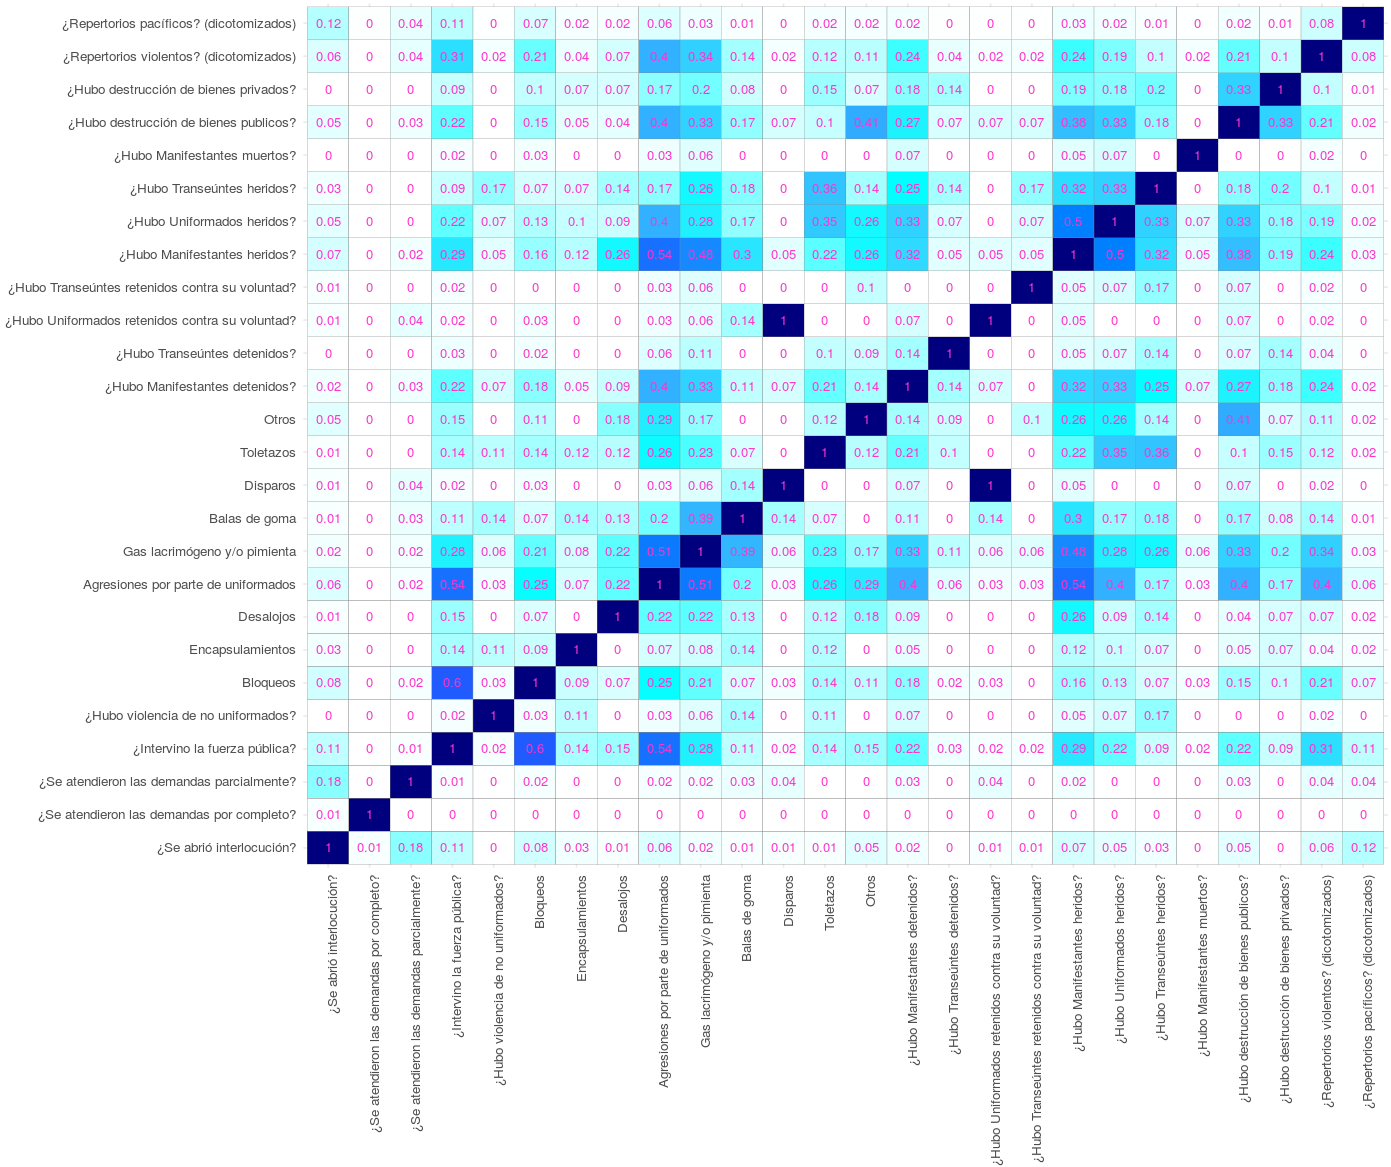
\includegraphics[scale=0.45]{img/3.24_simRespuestas.png}
\par
\small Fuente: Elaboración propia.
\end{minipage}\bigskip













% BEGIN                                                                                                                                                                  .                                                                                                                                                                  .                                                                                                                                                                        .                                                                                                                                                                 .                        CAPITULO 4: PANORAMA GENERAL (TIPOS DE ACTOR vs DEMANDAS y EPs)                                                                                 .                                                                                                                                                                  .                                                                                                                                                                        .                                                                                                                                                                 .                                                                                                                                                                        .                                                                                                                                                                 
\chapter{Red tripartita y agrupación de unidades sociales}
\label{chap:Redes_TiposActor}

\epigraph{\itshape Reductionism is merciless.}{---Douglas Hofstadter, \textit{I Am a Strange Loop}}

\begingroup
\small
    Este capítulo ofrece perspectivas generales sobre la estructura social en las coaliciones de eventos que constituyen nuestra evidencia. 
    Comenzamos por introducir la \emph{red 3-partita de eventos, actores y demandas} (sección \ref{sec:RedGeneral}), que representa el nivel más bajo de agregación en nuestros datos y se relaciona directamente con algunas observaciones del capítulo previo. 
    Posteriormente y a través de agrupaciones basadas en los objetivos ---o acciones--- principales de actores (incorporados a sectores amplios), pretendemos describir sus alianzas, dada una \emph{coparticipación sectorial ---y multisectorial---} en eventos (sección \ref{sec:RedAgregada_TiposEps}). 
    Por último, especificamos las \emph{relaciones discursivas entre sectores}, por las temáticas generales de las demandas a las que se les asocia durante un evento colaborativo (sección \ref{sec:RedProyectada_tiposCategorias}).
\vspace{2em}
\endgroup



Al inicio del capítulo \ref{chap:AnalisisDescriptivo} hemos descrito la orientación general de nuestra evidencia, deducida a partir de la evaluación panorámica sobre fuentes periodísticas, métodos y protocolos adoptados. 
Por el contenido de dicho capítulo, ahora podemos hacer algunas precisiones aún más específicas sobre la naturaleza de las unidades sociales relacionadas, sus tendencias y correlaciones anticipadas. 
Así, nuestros datos resultan caracterizables por dos aspectos clave prevalecientes en la cobertura periodística muestreada, que consideramos intervinientes en el análisis relacional de las coaliciones captadas: 
(i) por su \emph{tendencia ideológica}, la cual favorece en primer instancia, movimientos de organizaciones gremiales con alcance nacional ---especialmente de campesinos, maestros y sectores públicos sindicalizados--- y más concretamente, temáticas contextuales afines a la línea editorial de nuestra fuente periodística ---bajo ciclos de atención mediática sobre la \emph{reforma educativa} y la \emph{desaparición de los 43 normalistas de Ayotzinapa}---; 
y (ii) por una \emph{sobrerrepresentación geográfica}, centrada en unas cuantas ciudades del país ---principalmente Ciudad de México y Tuxtla Gutiérrez, aunque también (en menor medida) Chilpancingo de los Bravo y Acapulco de Juárez--- que difícilmente son representativas de todo el panorama nacional.


Donde tales sesgos se multiplican al replicarse a partir de referencias comunes en nuestra fuente y seguimientos asimétricos sobre eventos de protesta de larga duración. 
De modo que actores, demandas, repertorios y objetivos presentan una alta concentración, con cuantiosos eventos asociables a pocas categorías (y ausencia de categorías, para el caso de respuestas); reduciendo así la variabilidad de nuestras observaciones e implicando que otras caracterizaciones (especialmente de demandas, actores y lugares) resulten periféricas por sus frecuencias simples, con algunas superposiciones alrededor de estratos con mayor representación. 
Sin embargo, este reconocimiento también delimita nuestro objeto de estudio, lo que nos permite analizar con mayor claridad la estructura relacional dada por la convergencia de actores y temáticas peculiares en coaliciones acotadas, con relevancia contextual en un espacio determinado de difusión pública. 
En especial, reconocemos que la representación de estas coaliciones alude principalmente a una organización heterogénea, que forma oposiciones consistentes ante figuras políticas relevantes (nacionales y estatales) y que suele ser recibida con tolerancia y (en menor medida) con contención. 


Comenzamos este análisis con la descripción simple de la red 3-partita entre actores, eventos y demandas en la sección \ref{sec:RedGeneral}. 
Esta representación, de unidades singulares estáticas, pretende captar relaciones superpuestas (de actuación y discursivas) con tanta fidelidad como la fuente sugiere, de forma que se evitan agrupaciones más robustas. 
Como han sugerido \citet{2008_Nazir_TripartiteRelationships}, considerar varias unidades sociales relevantes al mismo tiempo reduce el aislamiento de subgrupos, permitiendo múltiples vínculos jerárquicos. 
Analizamos esta estructura social primordialmente a través de sus características topológicas básicas y la distribución de sus medidas de centralidad con el objetivo de esbozar una descripción panorámica. 


Ya que uno de nuestros objetivos en este capítulo es identificar coaliciones de eventos multisectoriales, analizamos en la sección \ref{sec:RedAgregada_TiposEps} (de forma agregada) los vínculos entre eventos y \emph{sectores}, donde se agrupan actores colectivos. 
Asumimos que estas relaciones ponderadas exhiben (así sea de forma parcial) la recurrencia con la que actores asociables a diversos movimientos se unen entre sí para protestar. 
Ya que hemos identificado frecuencias asimétricas de coparticipación en nuestros datos ---ver figura \ref{3.12_epsTipos}---, la descripción de esta red dividida en sectores revela el nivel de hermetismo entre grupos desiguales, así como la capacidad que tienen para movilizar (o ser adheridos) a coaliciones amplias de apoyo dentro de diferentes sectores. 


Otra dimensión analítica, que busca una posible persistencia en la agenda de actores agrupados, es deducida a través de \emph{relaciones discursivas}, que implica su adherencia a exigencias generales. 
De esta manera, presentamos en la sección \ref{sec:RedProyectada_tiposCategorias} una red de categorías agrupadas, en la que se recuperan relaciones indirectas ponderadas entre \emph{sectores} y \emph{clasificaciones de demandas}, por su presencia común en diferentes protestas colaborativas. 
Hemos separado su análisis bajo la precaución de que dichas relaciones deducidas no implican vinculaciones tácitas, debido a la multiplicidad de contextos (condicionados por el sesgo de nuestros datos) en los que se puede asociar a distintos sectores con categorías de demandas amplias. 




% BEGIN                                                                                                                                                          .                                                                                                                                                                        .                                              SECCIÓN 4.1 Red de eventos, actores y demandas                                                                    .                                                                                                                                                                        .                                                                                                                                                                .
\section{Red de eventos, actores y demandas}
\label{sec:RedGeneral}

La figura \ref{4.1_red_3partita} muestra la red 3-partita en la que se basa este trabajo; la cual relaciona tres tipos de unidades sociales, que consideramos elementales para explorar la representación de la protesta colaborativa: \emph{coaliciones de eventos} (583 unidades), \emph{actores colectivos identificados en la fuente} (432 unidades) y \emph{demandas únicas presentadas} (714 unidades), donde el tamaño de cada vértice es proporcional  a su grado simple y cada tipo de unidad social es diferenciada por un color propio\footnote{
    Se ha utilizado el algoritmo de \emph{Fruchterman-Reingold}, incorporado en el paquete \emph{qgraph} de \emph{R} para establecer posiciones relativas, tratando de reducir la superposición de aristas y manteniendo cerca vértices adyacentes. 
    El tamaño mínimo de cada vértice ha sido acotado para permitir su visualización. 
}. 



\hspace{-1em}\begin{minipage}{\linewidth}
\centering
\captionof{figure}{Red de eventos, actores y demandas (vértices proporcionales a su centralidad de grado).} \label{4.1_red_3partita}
\hspace{-1.6em}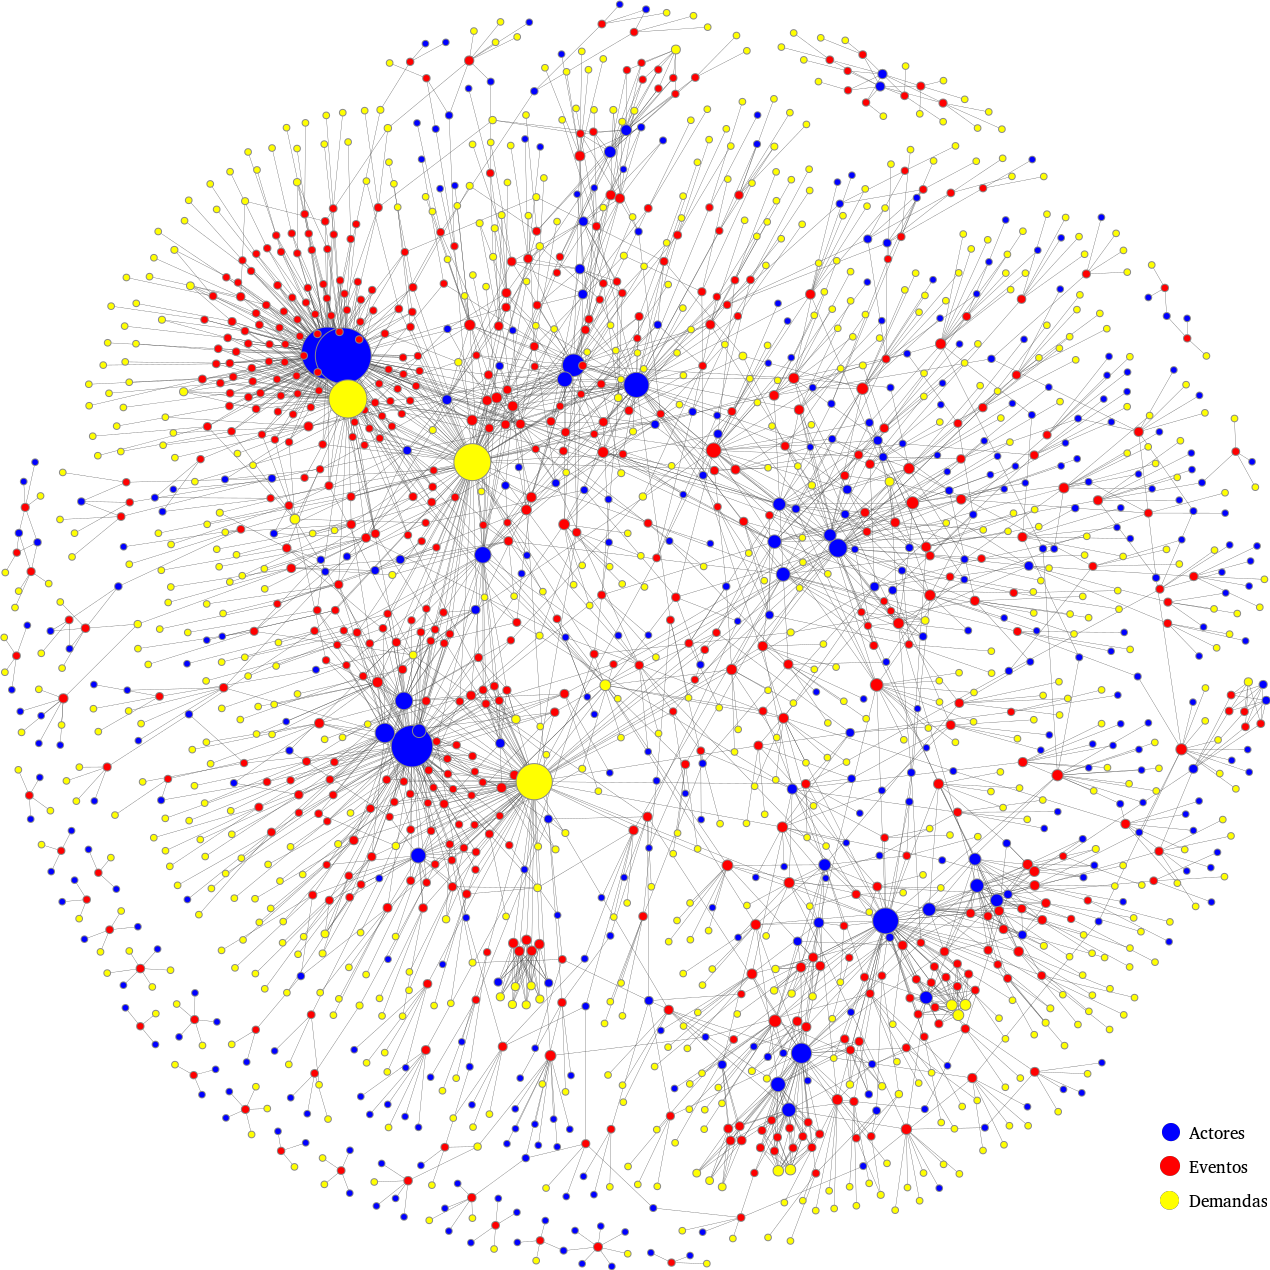
\includegraphics[scale=0.37]{img/4.1_red_3partita.png}
\par\bigskip
\small Fuente: Elaboración propia.
\end{minipage}\bigskip


Las demandas representadas en la figura \ref{4.1_red_3partita} son narrativas textuales particulares que han sido identificadas en nuestra fuente periodística, vinculadas de forma única a coaliciones específicas o replicadas en varios eventos a través de actividades paralelas, ciclos de protesta, continuidad temporal o uniformidad mediática. 
Constituyen un nivel distintivo, que podría ser agrupado en \emph{campañas} ---junto a eventos, como propone \citet{2003_Wada_Tesis}--- o \emph{clasificaciones temáticas} ---como de hecho se realiza en la sección \ref{sec:RedProyectada_tiposCategorias}---. 
Debido al filtro que opera en nuestra fuente, la mayoría de ellas ---y sobre todo las tres con mayor representación en eventos, como se ha indicado en el apartado de \nameref{subsubsec:demandas_textuales}-- refieren a la reforma educativa o la desaparición de los 43 normalistas de ayotzinapa; no obstante, múltiples temáticas periféricas con intereses más particulares son identificadas. 
Su tratamiento relacional nos permite detectar (más allá del recuento simple o por su superposición con otras características) relaciones discursivas en múltiples espacios, presentadas por diferentes coaliciones de actores; que reflejan un entorno múltiple y complejo sobre la representación de las exigencias captadas en nuestra muestra. 


En segundo lugar, los actores colectivos identificados incluyen múltiples datos covaribles, como se ha descrito en la sección \ref{sec:DatosOMS}; donde quizás el más interesante de ellos, por su capacidad para determinar coaliciones plurales es su \emph{sector} (asociados a sus objetivos o actividades principales) por lo que es utilizado de forma recurrente en este capítulo\footnote{
   Aunque en menor medida y dado el sesgo territorial detectado en el capítulo previo, también utilizamos (en el siguiente capítulo) el alcance regional de los actores para analizar la coherencia geográfica de las relaciones en nuestra red.  
}. 
Como se ha anticipado ---en la sección \ref{sec:actores}---, diversas causas pueden influir en la sobrerrepresentación de organizaciones gremiales de alcance nacional (lo cual les permite obtener una mayor centralidad de grado, según se observa en la figura \ref{4.1_red_3partita}): ya que quizás son más fácilmente identificables, cuentan con mayor influencia en la vida pública, estratos regionales, periodo analizado, redes de apoyo consolidadas y similaridad ideológica con nuestra fuente. 
Las relaciones que entre ellos se identifican son indirectas, y han sido determinadas por su afiliación común a eventos de protesta en los que han coparticipado; donde tal membresía (al ser definida de forma intencional, según la sección \ref{subsubsec:CoalicionesEventos}) señala pertenencia activa a un subgrupo, cuando menos de forma temporal, posicionándose de forma relativa a otros actores en nuestra red por las cadenas de eventos a las que se le ha relacionado. 


La predominancia de los eventos, aunque atenuada en nuestra red 3-partita, es preservada al referir la unidad de análisis principal en el diseño de investigación original. 
Por lo tanto, estos son los únicos vértices relacionados a los otros dos tipos de unidades sociales; cuyos vínculos son fijados en función de coparticipaciones (entre al menos dos actores nombrados) y motivaciones (una o más demandas reportadas). 
Cada una de estas \emph{coaliciones de eventos} incorpora implícitamente múltiples características adicionales que podrían trascender a su mera identificación abstracta\footnote{
    Las cuales también se podrían desagregar en otras unidades sociales, que permitiesen deducir relaciones adicionales entre eventos, de forma análoga a las \emph{demandas} y \emph{actores}.
}, como aquellas referidas en el capítulo \ref{chap:AnalisisDescriptivo}: respuestas a la protesta, repertorios utilizados para manifestarse, localización geográfica, duración del evento, tipo de cobertura mediática, instancias ante la cual se protesta y fechas (de ocurrencia y reportaje). 
No obstante, en la práctica tales características son excluidas con el fin de acotar nuestro objeto de estudio, ya que su análisis distintivo requeriría mejores datos, además de un tratamiento más detallado del que se ha decidido incluir en este retrato exploratorio. 
Como proponen \citet{1993_BrmanEvtt_StructureSocialProtest}, por medio del análisis de redes es posible detectar \emph{protestas exitosas}, en el sentido del establecimiento de una amplia red, que permite la resonancia de las demandas expresadas entre otros grupos e individuos; además, nos permite identificar continuidades entre eventos, por la articulación colaborativa de actores ---como señala \citet{2003_Diani_SocialNetworks}---. 
Tales reconocimientos ---en el ámbito de la protesta y dado el sesgo mediático--- son manifestados en la figura \ref{4.1_red_3partita} por las propiedades relacionales de las coaliciones muestreadas. 


A pesar de las posibilidades descriptivas que ofrece un examen minucioso de esta red, la exploración que se realiza de ella es superficial debido a la dificultad que representa su análisis relacional. 
De modo que sólo discutimos sus características topológicas más relevantes y las distribuciones de sus medidas de centralidad; posteriores agrupaciones y exclusiones a partir de esta red ahondarán en algunas particularidades estructurales adicionales. 



% BEGIN Sección 4.1.1

\subsection{Descripciones básicas}
\label{subsec:Descripcion}

Es usual que se analicen \emph{redes de afiliación} entre eventos y actores, bajo relaciones como las que exhibimos en la red de la figura \ref{4.1_red_3partita}. 
La composición de coaliciones de organizaciones discretas (particularmente aquellas de alcance nacional, sin una alta especificidad de sección o región) expresan relaciones episódicas de colaboración que en conjunto pueden trascender localidades particulares y exhibir pautas recurrentes de actuación entre subconjuntos de actores. 
Al incorporar demandas con una gran resonancia a tal red bipartita (aún teniendo en cuenta la especificidad de las narrativas textuales utilizadas) creamos nexos discursivos que dan continuidad a las temáticas expresadas entre coaliciones. 
Aunque de diferente tipo, estas relaciones simultáneas establecen una estructura social simbólica, robusta y de trayectorias múltiples entre las unidades sociales conectadas en nuestra red 3-partita. 



Aún así existen 20 componentes en la red, lo cual resulta en el aislamiento de ciertas protestas, sus demandas y actores vinculados. 
Quince de estas componentes se integran de un solo evento colaborativo; donde ninguno de sus actores colectivos o demandas textuales identificadas vuelven a tener representación mediática en otras coaliciones de eventos en el periodo analizado\footnote{
    Este aislamiento podría ser explicado en algunos casos por la diferenciación de las organizaciones referidas ---por ejemplo, el \emph{Frente Nacional por la Familia} y \emph{la Red Guerrero Por La Vida}---; la especificidad de las tareas que llevan a cabo ---\emph{Colectivo Solecito de Veracruz} y \emph{Red de Madres de Hijos desaparecidos}---; una alta especificidad en las demandas que se consignan; una poca coparticipación en coaliciones; ostracismo mediático u organizativo y debido a la mínima cobertura que reciben ciertas zonas del país. 
}. 
En tres componentes más existe una o dos organizaciones que permiten relacionar de dos a tres eventos de protesta, bajo diferentes niveles de coherencia\footnote{
    La \emph{Confederación Revolucionaria de Obreros y Campesinos} (CROC), al ser una agrupación con fuerte presencia nacional relaciona dos eventos en una de estas componentes pequeñas, cuya vinculación podría ser debatible por el contenido de sus demandas y una evidente diferenciación regional; donde un evento es registrado en el Estado de México y otro en Baja California Sur. 
    Los otros dos casos resultan más compatibles por la especificidad de las agrupaciones, que vinculan dos eventos locales ---en el caso de \emph{\#YoSoy132 (sección San Luis Potosí)}---, y tres ---para los Sindicatos \emph{de Trabajadores al Servicio del Poder Judicial} y \emph{Legislativo de Morelos}; (SUTSPJ) y (SUTSPLEM) respectivamente---. 
}. 
Una componente más que permanece aislada reúne ocho eventos; sin embargo, los únicos dos grupos que se adhieren a ellos son coordinados en caravanas anuales\footnote{
    Esta es la \emph{Caravana Liberando la Esperanza}, que esta conformada por madres de migrantes en búsqueda de sus familiares desaparecidos en el país y cuya organización es asistida por el \emph{Movimiento Migrante Mesoamericano} (MMM). 
    A pesar de que hay cierta unidad en su conformación, estos actores han sido referidos de forma distintiva en otros eventos dentro de nuestra fuente periodística, motivo por el cual fueron considerados de forma independiente en nuestros datos. 
}. 
Finalmente, nuestra \emph{componente principal} agrupa 1601 unidades sociales, incluyendo a los actores y demandas con mayor presencia en nuestros datos. 



En el recuento anterior ---y sobre todo para la componente principal--- la inducción de relaciones entre eventos no siempre implica una coherencia impecable, sino una mera replicación en la identificación de al menos un actor o demanda, que conecte eventos (de otra forma dispersos) a través del fragmento de la esfera pública considerado; por tanto (como se ha indicado en la sección \ref{sec:Fuente_EPs}) no sólo las características de la protesta modelan esta estructura social, sino también los sesgos del medio periodístico que la representa y nuestras mediciones sobre esta unidad de análisis. 
Como también señalamos en la sección \ref{sec:cobertura}, descripciones detalladas sobre eventos en nuestra fuente periodística permiten una caracterización mucho más precisa de sus unidades sociales, mientras que el registro de varios eventos de características similares o ambiguas resulta en un sesgo de representación desproporcional, que otorga una mayor conectividad a actores y demandas destacadas. 


Además de la prominencia relativa que es posible observar en algunas unidades sociales representadas en la figura \ref{4.1_red_3partita} (a través de su grado simple) sobresale la formación de bicliques (subgrafos bipartitos completos maximales, formados por las relaciones ---a menudo simultáneas--- entre \emph{eventos-demandas} y \emph{eventos-actores}). 
Ambas características son consecuencia de los sesgos detectados en el capítulo anterior, cuyo impacto es persistente en cada uno de los grafos derivados que se presentan en este capítulo y el siguiente. 



\subsubsection{Características de la componente principal}
\label{subsubsec:Características_Cppal}

Dada la aglomeración de unidades sociales relacionadas en la componente principal de nuestra red 3-partita, describimos a continuación algunas de sus características topológicas básicas (definidas en la sección \ref{sec:Caracteristicas}): 

\begin{description}
    \setlength\itemsep{0em}
    \item[Diámetro:] Es decir, la mayor distancia entre cualquier par de vértices, es dada por un camino de longitud 12.
    \item[Periferia:] Esta compuesta por 47 demandas textuales únicas y 32 actores colectivos con una baja representatividad\footnote{
	Es decir, que la mayor parte de los actores y demandas que figuran en la periferia sólo fueron vinculados a unos cuantos eventos. 
    }. 
    \item[Radio:] La distancia mínima de un vértice a cualquier otro en la componente, es de 6. 
    \item[Centro:] Se compone únicamente de la demanda por la \emph{presentación con vida de los 43 normalistas de ayotzinapa desaparecidos}, al ser esta una exigencia ampliamente extendida en múltiples espacios. 
    \item[Distancia media entre vértices $\ell$:] 5.73 (según la ecuación \ref{dist_media_1c})\footnote{
	Y 5.97 para $\ell'$, considerando todas las componentes (de acuerdo a la ecuación \ref{dist_media_mc}). 
    }. 
\end{description}



Las características descritas muestran que pese a la gran cantidad de unidades sociales incluidas en la componente principal y aún exceptuando la proyección de relaciones indirectas entre vértices del mismo tipo, la \emph{distancia social}\footnote{
    Entendida como el mínimo número de relaciones simbólicas requeridas para conectar dos unidades sociales. 
} 
que separa a cualquier par de vértices es generalmente bastante pequeña. 
Lo cual puede ser indicio de los límites en el espacio de representación de la vida pública que tiene cabida en nuestra fuente ---dada su agenda política y sesgo regional--- donde (a pesar de la exclusión de un número relativamente menor de eventos, actores y narrativas) cuantiosas manifestaciones plurales pueden ser articuladas alrededor de estratos de mayor conmoción. 


Sin embargo, es importante recordar que la retrospectiva que se presenta es de carácter acumulado, lo cual puede extender el alcance real de las unidades relacionadas. 
De tal modo que la ventana temporal a la que nos asomamos permite acoplar distintos escenarios contextuales, a partir de los que se genera un visión panorámica de carácter mediático en el periodo; particiones anuales sobre esta red muestran un escenario fragmentado. 
Por otro lado, proyecciones efectuadas reducirán aún más las distancias entre unidades sociales individuales; y, al descartar las demandas (como se muestra en la red de la figura \ref{5_1_red_actores_eventos}) la componente principal perderá conectividad. 



\begin{minipage}{\linewidth}
\centering
\captionof{figure}{Histograma de excentricidades en la componente principal.} \label{4.2_hist_excentricidades}
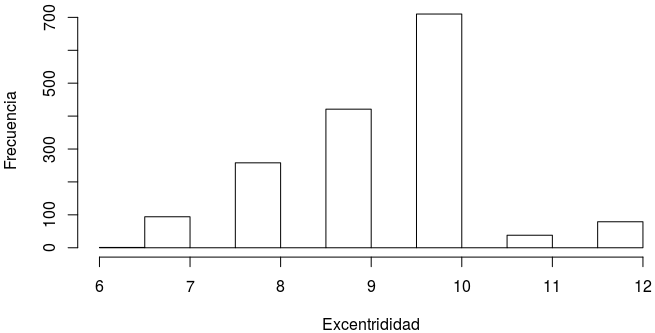
\includegraphics[scale=0.6]{img/4.2_hist_excentricidades.png}
\par\bigskip
\small Fuente: Elaboración propia.
\end{minipage}\bigskip






% BEGIN Sección 4.1.2

\subsection{Medidas de centralidad}
\label{subsec:Centralidad_3part}

El cúmulo de relaciones inferidas conforman una \emph{estructura social}, que teóricamente manifiesta oportunidades y restricciones para la acción colaborativa (en el caso de actores) o propagación (para demandas) dentro de las fronteras ---sociales y mediáticas--- representadas. 
Donde algunas de estas \emph{condiciones de entorno} pueden ser deducidas al determinar posiciones de importancia relativa. 


Presentamos una aproximación general sobre tales posiciones calculando y sintetizando las medidas de centralidad introducidas en la sección \ref{subsec:centralidades}\footnote{
    No obstante, descartamos la centralidad de Katz dada su alta correlación con la centralidad de vector propio y ya que esta medida no resulta aplicable a nuestra red 3-partita 
    (toda vez que el factor de atenuación $\alpha$ supone caminos incidentes a unidades sociales del mismo tipo).
}. 
Donde la proporción $n_{x}$ de unidades sociales del mismo tipo con cierta centralidad $x$ es presentada en sendas distribuciones. 



\subsubsection{Centralidades de grado}
\label{subsubsec:Centralidades_grado_3part}

La \emph{centralidad de grado} en nuestra red (representada de forma aproximada en la figura \ref{4.1_red_3partita}) refiere los siguientes conteos simples: 
(i) coparticipaciones documentadas en coaliciones de eventos ---centralidad de grado de \emph{actores}---; 
(ii) protestas en las que se reportó una misma expresión textual ---centralidad de grado de \emph{demandas}---; 
y (iii) número de actores y demandas que han sido involucrados en una coalición ---centralidad de grado de \emph{eventos}---. 
Aunque estas centralidades conllevan interpretaciones propias, de acuerdo a la unidad social a la que hacen referencia; en general, las unidades sociales con una alta centralidad de grado (por la concentración de vínculos incidentes) gozan de mayor reconocimiento y popularidad en un entorno particular de la red, implicando una mayor influencia local y capacidad de representación directa en el espacio público asociado a nuestra fuente. 


Algunos de estos recuentos ya han sido referidos en términos absolutos en el capítulo previo (ver figuras \ref{3.10_distribucionActores}, \ref{3.11_participacionesxActor} y tabla \ref{Actores_con_mayorPresencia}). 
No obstante, aquí nos centramos en la \emph{distribución de grado} de cada unidad social, de acuerdo a la ecuación \ref{eq:distribucion_grado}. 
Atendiendo las precauciones de \citet{2009_PowerLaw_Clauset_EtAl} ---dada su dispersión y las pocas observaciones que ha sido posible obtener---, resulta discutible estimar cierta bondad de ajuste bajo la hipótesis de una distribución de grado particular, por lo tanto nos limitamos a presentar su descripción general. 



La distribución de grado de actores (figura \ref{4.3_grado_actores}) se puede considerar una normalización del conteo simple de la figura \ref{3.11_participacionesxActor}; cuyo sesgo es evidente\footnote{
    Sobresalen (en el extremo superior izquierdo de la figura \ref{4.1_red_3partita}) las secciones 7 y 40 de la \emph{CNTE} (en Chiapas), donde sólo ellas colaboran en 121 eventos colaborativos. 
    Más interesantes por la diversidad de los actores que coparticipan con ellos, son los casos de la \emph{CETEG}, \emph{CNPA-MLN}, \emph{CNTE-22}, \emph{CNTE-18}, \emph{Barzón}, \emph{MPG}, \emph{SME}, \emph{SUSPEG} y \emph{CNTE-14}. 
} y está relacionado a nuestra discusión de la sección \ref{sec:actores}. 
Por su forma, se podría sugerir un ajuste a una distribución libre de escala; no obstante, al representarse en escalas logarítmicas, es fácil apreciar las irregularidades que podrían surgir al intentar hacer dicho ajuste para $k > 10$. 


\begin{minipage}{\linewidth}
\centering
\captionof{figure}{Distribución de grado de actores (escalas normales y logarítmicas).} \label{4.3_grado_actores}
\hspace{-1em}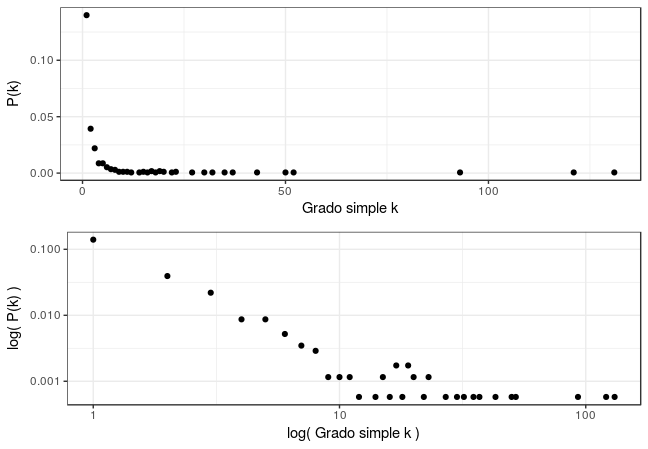
\includegraphics[scale=0.75]{img/4.3_grado_actores.png}
\par
\small Fuente: Elaboración propia.
\end{minipage}\bigskip


Las distribuciones de grado (diferenciadas para cada unidad social) son mostradas en la figura \ref{4.4_distribuciones_grado}. 
Donde comprobamos que la distribución de demandas resulta mucho más asimétrica, de modo que sólo unas pocas de ellas pueden ser vinculadas a más de un evento dada su especificidad. 
Esta irregularidad ya ha sido discutida en la sección \ref{sec:demandas}, donde su temática (en especial para las tres demandas con mayor representación) es consistente con las olas de protestas identificadas. 


Por último, la distribución de grado de eventos es condicionada por una alta especificidad periodística, lo cual revela su importancia relativa en este espacio. 
Por el reducido número de actores y demandas identificados en cada coalición, esta centralidad tiene un menor rango que aquél correspondiente a actores y demandas: 173 eventos tienen una centralidad mínima ($k=3$) y la máxima centralidad ($k=23$) es aplicable a una sola coalición. 
Aquellos eventos con un alto grado relativo corresponden a coaliciones amplias entre múltiples actores colectivos, donde se expresaron una gran variedad de demandas significativas. 
La mayoría relacionada por un eje común que refiere los motivos de dicha coalición: 
anular las reformas estructurales (3 EPs, con $k=23$, $k=16$ y $k=14$); 
en contra de acuerdos comerciales internacionales (1 EPs, con $k=17$); 
solicitud de asignación de recursos públicos a un sector (1 EPs, con $k=16$); 
o en oposición a la sobreexplotación de recursos territoriales (2 EPs, con $k=13$). 

\begin{minipage}{\linewidth}
\centering
\captionof{figure}{Distribuciones de grado de actores, eventos y demandas.} \label{4.4_distribuciones_grado}
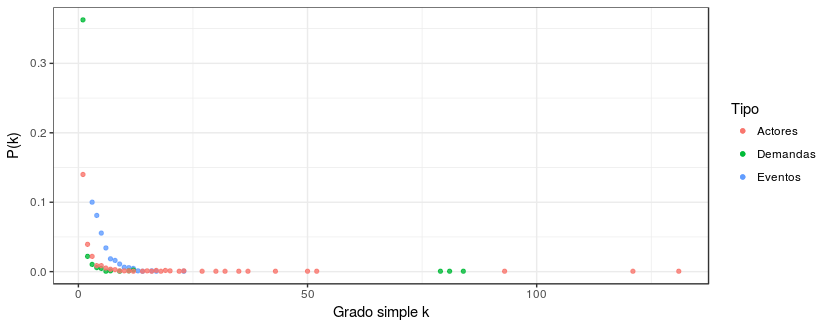
\includegraphics[scale=0.7]{img/4.4_distribuciones_grado.png}
\par
\small Fuente: Elaboración propia.
\end{minipage}\bigskip

El sesgo en estas tres distribuciones es convergente con otros sesgos de representatividad descritos y consistente con lo esperado en redes sociales simples ---de actores relacionados---, donde pocos vértices poseen un grado superior, ocasionalmente achacado al \emph{apego preferencial} de nuevos vértices por conectarse con otros bien posicionados. 
En nuestro caso particular, creemos que una parcial explicación sobre estos sesgos basada en dicho apego podría ser sugerente (particularmente en el caso de las demandas más populares, cuya proclamación puede favorecer la articulación mediática y social de eventos diversos). 
No obstante, actores y demandas con un grado mayor a la media no necesariamente suponen preferencias ampliamente extendidas en el ámbito de las coaliciones de eventos; sino también una monopolización de recursos, creación de consensos y un mayor peso de representación mediática. 



\subsubsection{Centralidades de intermediación}
\label{subsubsec:Centralidades_intermediacion_3part}


Preservando las posiciones determinadas en la figura \ref{4.1_red_3partita}, representamos en la figura \ref{4_5_cIntermediacion} la red 3-partita, donde el tamaño relativo de cada unidad social es proporcional a su \emph{centralidad de intermediación}. 


Esta centralidad es relevante al identificar \emph{unidades sociales de convergencia}; interdependientes, dadas las afiliaciones entre eventos, actores y demandas en la red. 
Aunque matemáticamente su cálculo (de acuerdo a la ecuación \ref{eq:intermediacion}) es equivalente para cada vértice, un alto índice relativo puede ser interpretable en diferentes términos para cada unidad social, siendo asociado a: 
(i) hitos de confluencia ideológica u organizacional ---intermediación de \emph{eventos}---; 
(ii) puentes discursivos ---intermediación de \emph{demandas}---; 
o (iii) organizaciones que median una gran cantidad de relaciones simbólicas entre subgrupos acotados ---intermediación de \emph{actores}---. 


A pesar de que existe una alta correlación de Pearson entre la centralidad de grado e intermediación ($r = 0.7955758$), se observan diferencias sustanciales entre sus distribuciones ---ver figuras \ref{4.4_distribuciones_grado} y \ref{4.6_distribuciones_intermediacion}---. 
En especial, se identifica el papel central que guardan pocas demandas como conectores en la red, así como una menor asimetría en la centralidad de actores. 
Las tablas \ref{Actores_con_mayor_CB} y \ref{Demandas_con_mayor_CB} muestran a los 20 actores y demandas con mayor intermediación respectivamente. 

\newpage
\hspace{-1.5em} \begin{minipage}{\linewidth}
\centering\bigskip
\captionof{figure}{Red de eventos, actores y demandas (vértices proporcionales a su centralidad de intermediación).} \label{4_5_cIntermediacion}
\includepdf[pages={1},scale=0.95,pagecommand={},offset=5 70]{img/4_5_cIntermediacion.pdf}
\includegraphics[scale=0.1]{img/null.png}
\vspace{36em}
\par\bigskip
\small Fuente: Elaboración propia.
\end{minipage}\bigskip



Esta información revela que es en las demandas (más que en los actores), donde recae gran parte de la articulación de eventos en la red. 
Más específicamente, que aquellas exigencias con una fuerte difusión (repetidas a manera de eslogan), a pesar de su limitada superposición, se ostentan como centros aglutinantes contiguos con capacidad para reforzar y propagar agendas específicas en múltiples espacios; a partir de los cuales se podrían sostener movimientos amplios desde diferentes frentes, más allá de los que son capaces de articular actores o sectores demarcados ---por sus propias acciones agregadas, usualmente confinadas a ambientes locales---. 
Dado el papel secundario que usualmente es otorgado a las demandas en otros análisis descriptivos sobre movimientos sociales (donde el énfasis es puesto casi exclusivamente en las acciones de manifestantes singulares o agrupados), deducimos un alto potencial heurístico en el rastreo de la tematización de tales unidades sociales como puentes discursivos. 


\begin{minipage}{\linewidth}
\centering
\captionof{figure}{Distribuciones de intermediación de actores, eventos y demandas.} \label{4.6_distribuciones_intermediacion}
\includegraphics[scale=0.7]{img/4.6_distribuciones_intermediacion.png}
\par
\small Fuente: Elaboración propia.
\end{minipage}\bigskip


\begin{table}[!hbt]
\center
\scriptsize
\caption{Demandas con mayor centralidad de intermediación.}
\label{Demandas_con_mayor_CB}
\begin{tabular}{ | l | c | } 
\hline
\hspace{19em} \textbf{Demanda} & \textbf{$C_{B}(i)$}\\
\hline
[a favor] presentación con vida de los 43 normalistas de ayotzinapa desaparecidos & 338,476.2\\ \hline
[en contra] reforma educativa & 211,837.8\\ \hline
[a favor] abrogación de la reforma educativa & 120,455.1\\ \hline
[a favor] liberación de los presos políticos & 53,444.1\\ \hline
[a favor] mejoras salariales & 16,481.4\\ \hline
[en contra] feminicidios & 12,006.6\\ \hline
[a favor] renuncie el presidente enrique peña nieto & 6,384.0\\ \hline
[a favor] mesa de diálogo nacional por reforma educativa & 6,133.3\\ \hline
[a favor] renuncia del secretario de educación, aurelio nuño mayer & 5,623.3\\ \hline
[en contra] reforma educativa y sus leyes secundarias & 4,791.0\\ \hline
[en contra] reforma laboral & 3,556.4\\ \hline
[en contra] ley de servicio profesional docente (reforma educativa) & 2,745.9\\ \hline
[en contra] evaluación docente por reforma educativa & 2,220.2\\ \hline
[a favor] cese de la represión & 1,955.2\\ \hline
[en contra] comicios & 1,363.1\\ \hline
[en contra] propuesta para aplicar el impuesto al valor agregado a los alimentos & 999.6\\ \hline
[en contra] reforma energética & 978.5\\ \hline
[en contra] reformas estructurales & 933.6\\ \hline
[a favor] liberación de los líderes de la sección 22 de la CNTE, en su lucha por la reforma educativa & 609.2\\ \hline
[a favor] renuncia de la secretaria de educación en el estado, esthela gutiérrez & 441.6\\ \hline
\end{tabular}
\par\bigskip
\caption*{\small Fuente: Elaboración propia.}
\end{table}



\begin{table}[!hbt]
\center
\scriptsize
\caption{Actores colectivos con mayor centralidad de intermediación.}
\label{Actores_con_mayor_CB}
\begin{tabular}{ | l | c | } 
\hline
\hspace{19em} \textbf{Actor} & \textbf{$C_{B}(i)$}\\
\hline
Coordinadora Nacional Plan de Ayala - Movimiento de Liberación Nacional (CNPA-MLN) & 188,954.0\\ \hline
Coordinadora Estatal de los Trabajadores de la Educación de Guerrero (CETEG) & 143,505.4\\ \hline
Coordinadora Nacional de Trabajadores de la Educación (SNTE – CNTE) – Sección 22 & 139,216.9\\ \hline
Sindicato Mexicano de Electricistas (SME) & 130,770.1\\ \hline
Coordinadora Nacional de Trabajadores de la Educación (SNTE – CNTE) – Sección 7 & 124,121.7\\ \hline
Coordinadora Nacional de Trabajadores de la Educación (SNTE – CNTE) – Sección 18 & 101,048.3\\ \hline
Sindicato de Telefonistas de la República Mexicana (STRM) & 86,651.9\\ \hline
Coordinadora Nacional de Trabajadores de la Educación (SNTE – CNTE) – Sección 40 & 77,569.1\\ \hline
El Barzón Popular – Unión Nacional Barzonista & 72,482.5\\ \hline
Coordinadora Nacional de Trabajadores de la Educación (SNTE – CNTE) – Sin sección identificada & 66,594.4\\ \hline
Coordinadora Nacional de Trabajadores de la Educación (SNTE – CNTE) – Sección 14 & 51,507.1\\ \hline
Frente Popular Francisco Villa (FPFV) & 41,281.2\\ \hline
Unión Nacional de Trabajadores (UNT) & 40,900.1\\ \hline
Sindicato de Trabajadores de la Universidad Nacional Autónoma de México (STUNAM) & 33,630.9\\ \hline
Movimiento Popular Guerrerense (MPG) & 29,373.8\\ \hline
\#YoSoy132 – Sección Ciudad de México & 26,587.9\\ \hline
Unión Nacional de Trabajadores Agrícolas (UNTA) & 21,349.7\\ \hline
Central Campesina Cardenista (CCC) & 20,083.5\\ \hline
Frente Indígena y Campesino de México (FICAM) & 19,978.7\\ \hline
Coordinadora Nacional de Trabajadores de la Educación (SNTE – CNTE) – Sección 36 & 18,742.2\\ \hline
\end{tabular}
\par\bigskip
\caption*{\small Fuente: Elaboración propia.}
\end{table}


Por otro lado, se destaca el posicionamiento de organizaciones corporativistas, quienes acoplan escenarios territorialmente heterogéneos. 
Es decir, que gran parte de los grupos con una alta intermediación mantienen relaciones cercanas con actores locales (que pueden ser asociados a los mismos estados en los que ellos sostienen sus actividades); a la vez que establecen relaciones coyunturales con actores foráneos o de mayor alcance. 
También observamos que algunas de estas organizaciones ---principalmente campesinos y maestros--- son intermediarios sectoriales, dada la flexibilidad de algunas de sus alianzas y los vínculos recurrentes que guardan con agrupaciones similares. 
En conjunto, tales relaciones participativas asequibles permiten reunir escenarios relativamente fragmentados (sectorial o geográficamente). 
Así mismo, el hecho de que la mayoría de estos actores hayan expresado las demandas con mayor centralidad de intermediación de forma recurrente no es incidental; al hallar de forma simultánea los caminos más cortos que separan a cualquier par de vértices (independientemente de si se trata de eventos, actores o demandas) superponemos diferentes tipos de relaciones simbólicas, de modo que estos resultados deben entenderse en su conjunto. 
Finalmente, a diferencia de lo propuesto por \citet{2003_Wada_Tesis}, en este nivel ninguna ONG individual aparece entre los actores con mayor capacidad de interconexión\footnote{
    Aunque una justa comparación ameritaría una agrupación sectorial que excluyese demandas, la cual podría ser hasta cierto punto equiparable con nuestra red de la próxima sección. 
}. 


Cabe mencionar que el alcance potencial de una unidad social con gran intermediación podría ser circunstancial y de especial trascendencia en oportunidades contextuales particulares. 
Donde subgrupos de vértices relativamente aislados sean integrados a un espacio de representación amplio principalmente (aunque no exclusivamente) por estas unidades intermediarias que medien relaciones indirectas ---simbólicas---.
Dado el papel protagónico de actores y demandas ligadas a las temáticas principales en nuestra base de datos, suponemos que estos movimientos se incrustan como núcleos de enlace, que controlan la discusión pública entorno a la protesta política (acotada en un espacio mediático) y  alrededor de los cuales se articulan protestas periféricas. 



\subsubsection{Centralidades de cercanía}
\label{subsubsec:Centralidades_cercania_3part}

La centralidad de cercanía ha sido calculada de acuerdo a la ecuación \ref{eq:cercaniaAjustada2}, debido a que nuestra red incluye más de una componente. 
Su distribución (ver figura \ref{4.7_distribuciones_cercania}) muestra una clara división en dos grupos: unidades sociales en pequeñas componentes y unidades sociales en la componente principal. 
Como se ha anticipado en la sección \ref{subsubsec:OtrasDistribucionesCentralidad}, esta distribución no resulta tan sesgada como las otras, dada la pequeña distancia que une a la mayoría de vértices (en especial dentro de la componente principal ---ver figura \ref{4.2_hist_excentricidades}---). 


\begin{minipage}{\linewidth}
\centering
\captionof{figure}{Distribuciones de cercanía de actores, eventos y demandas.} \label{4.7_distribuciones_cercania}
\includegraphics[scale=0.7]{img/4.7_distribuciones_cercania.png}
\par
\small Fuente: Elaboración propia.
\end{minipage}\bigskip


Las unidades sociales con mayor centralidad de cercanía (es decir, aquellas que son más cercanas al centro de red y pueden ser conectadas con múltiples vértices a través de un camino relativamente corto) teóricamente tienen una mayor efectividad potencial en procesos dinámicos debido a la \emph{accesibilidad} que tienen hacia otros vértices. 
Como  en el caso anterior, los 20 actores y demandas con mayor centralidad de cercanía son señalados en las tablas \ref{Actores_con_mayor_CC} y \ref{Demandas_con_mayor_CC} respectivamente. 


\begin{table}[!hbt]
\center
\scriptsize
\caption{Actores colectivos con mayor centralidad de cercanía.}
\label{Actores_con_mayor_CC}
\begin{tabular}{ | l | c | } 
\hline
\hspace{19em} \textbf{Actor} & \textbf{$C_{B}(i)$}\\
\hline
Coordinadora Nacional de Trabajadores de la Educación (SNTE – CNTE) – Sección 7 & 498.5\\ \hline
Coordinadora Nacional de Trabajadores de la Educación (SNTE – CNTE) – Sección 40 & 483.6\\ \hline
Coordinadora Estatal de los Trabajadores de la Educación de Guerrero (CETEG) & 482.3\\ \hline
Coordinadora Nacional de Trabajadores de la Educación (SNTE – CNTE) – Sección 22 & 463.7\\ \hline
Coordinadora Nacional de Trabajadores de la Educación (SNTE – CNTE) – Sección 18 & 460.4\\ \hline
Sindicato de Telefonistas de la República Mexicana (STRM) & 458.8\\ \hline
Sindicato Mexicano de Electricistas (SME) & 453.2\\ \hline
Coordinadora Nacional Plan de Ayala - Movimiento de Liberación Nacional (CNPA-MLN) & 439.8\\ \hline
Coordinadora Nacional de Trabajadores de la Educación (SNTE – CNTE) – Sección 14 & 435.9\\ \hline
Sindicato de Trabajadores de la Universidad Nacional Autónoma de México (STUNAM) & 434.2\\ \hline
Unión Nacional de Trabajadores (UNT) & 426.6\\ \hline
Movimiento Popular Guerrerense (MPG) & 417.3\\ \hline
Coordinadora Nacional de Trabajadores de la Educación (SNTE – CNTE) – Sección 9 & 415.2\\ \hline
Coordinadora Nacional de Trabajadores de la Educación (SNTE – CNTE) – Sin sección identificada & 412.4\\ \hline
Sindicato Único de Trabajadores del Colegio de Bachilleres (SUTCOBACH) – Sección Guerrero & 400.7\\ \hline
Sindicato Único de Servidores Públicos del Estado de Guerrero (SUSPEG) & 399.1\\ \hline
El Barzón Popular – Unión Nacional Barzonista & 393.0\\ \hline
Frente Popular Francisco Villa (FPFV) & 388.7\\ \hline
Coordinadora Nacional de Trabajadores de la Educación (SNTE – CNTE) – Sección 36 & 384.4\\ \hline
\makecell[l]{Sindicato Nacional de Trabajadores Mineros, Metalúrgicos, Siderúrgicos \\y Similares de la República Mexicana (SNTMMSSRM) – Sin sección identificada} & 380.8\\ \hline
\end{tabular}
\par\bigskip
\caption*{\small Fuente: Elaboración propia.}
\end{table}


A pesar de la baja correlación con las dos centralidades descritas anteriormente, gran parte de las demandas y actores con mayor grado e intermediación también se destacan aquí. 
Específicamente, como mencionamos en las \nameref{subsubsec:Características_Cppal}, el centro de las unidades relacionadas esta constituido únicamente por la demanda sobre la \emph{presentación con vida de los 43 normalistas de ayotzinapa desaparecidos}. 
A pesar de que esta exigencia se sostiene por menos tiempo que el movimiento de maestros (\emph{contra la reforma educativa}), la primer demanda se puede considerar más incluyente y hegemónica por la accesibilidad de relaciones colaterales que se permiten desde el corazón de esta representación. 


\begin{table}[!hbt]
\center
\scriptsize
\caption{Demandas con mayor centralidad de cercanía.}
\label{Demandas_con_mayor_CC}
\begin{tabular}{ | l | c | } 
\hline
\hspace{19em} \textbf{Demanda} & \textbf{$C_{B}(i)$}\\
\hline
[a favor] presentación con vida de los 43 normalistas de ayotzinapa desaparecidos & 517.9\\ \hline
[a favor] abrogación de la reforma educativa & 483.3\\ \hline
[en contra] reforma educativa & 478.2\\ \hline
[a favor] liberación de los presos políticos & 426.6\\ \hline
[a favor] apertura de una mesa de diálogo con el gobierno federal & 349.3\\ \hline
[a favor] cambio del rumbo económico del país & 347.5\\ \hline
[a favor] derogación de reforma laboral & 347.5\\ \hline
[a favor] freno de las agresiones del gobierno contra los obreros & 347.5\\ \hline
[a favor] solución al caso mexicana de aviación & 347.5\\ \hline
[a favor] transformación del pacto por méxico, tiene que ser también social & 347.5\\ \hline
[a favor] abrogación de todas las reformas estructurales, en particular la reforma educativa & 344.7\\ \hline
[a favor] libertad de los presos políticos, que ya suman 14 en este sexenio & 344.7\\ \hline
[en contra] ley de servicio profesional docente (reforma educativa) & 343.6\\ \hline
[en contra] reforma laboral & 342.6\\ \hline
\makecell[l]{[a favor] gobierno federal fije su postura ante el intento de charrazo de la cúpula del SNTE,\\ pues desde el lunes pasado pretende imponer una comisión ejecutiva al frente de la sección 9} & 342.1\\ \hline
[a favor] reanudación de las negociaciones con los gobiernos estatales & 342.1\\ \hline
[a favor] de la estabilidad laboral & 341.5\\ \hline
\makecell[l]{[en contra] sesgo informativo y la política editorial de agresión y desprestigio de televisa \\y tv azteca contra el movimiento que se opone a la reforma educativa} & 339.7\\ \hline
[a favor] renuncia del secretario de educación, aurelio nuño mayer & 338.9\\ \hline
[a favor] justicia y el esclarecimiento de los hechos (por desaparición de los 43 normalistas) & 338.3\\ \hline
\end{tabular}
\par\bigskip
\caption*{\small Fuente: Elaboración propia.}
\end{table}


Interpretamos esta accesibilidad principalmente en términos de constitución ideológica (en el caso de demandas) e inserción simbólica (de actores que se desempeñan como portavoces) en tales contextos. 
Dados los ciclos de atención mediática y de protesta que hemos asumido, suponemos que es a partir de ellos ---en conjunto con otros sesgos sistemáticos--- que se crea esta estructura social concurrente. 
Por otro lado, ya que nuestra evidencia recopila información de forma asimétrica sobre estos movimientos y hemos detectado que son ellos quienes articulan diferentes segmentos de la red, resulta consistente que estas unidades sociales dominen también la proximidad con otros eventos (aunque, en general, las unidades sociales con altas centralidades de estos tres tipos no tienen porque ser coincidentes). 




\subsubsection{Centralidades de vector propio}
\label{subsubsec:Centralidades_vector_3part}

Ya que la centralidad de vector propio considera de forma recursiva las relaciones en la red, es capaz de detectar el centro de subgrupos cohesivos de vértices significativos. 
En nuestra red 3-partita esto equivale a determinar aquellas unidades sociales con mayor incidencia global en el contexto superpuesto dado por demandas, actores y eventos. 

La figura \ref{4.8_distribuciones_eigenvector} muestra su distribución, donde se puede apreciar que sólo unas pocas unidades tienen una alta centralidad. 
Ellas corresponden a dos actores (secciones 7 y 40 de la \emph{CNTE}, en Chiapas), las coaliciones en las que han participado y sus principales demandas (\emph{[a favor] abrogación de la reforma educativa} y \emph{[en contra] reforma educativa}). 


Debido a los sesgos en su registro ---referidos en la sección \ref{sec:EPs largos}---, la persistencia de colaboraciones entre estos dos actores y el reforzamiento con el que se articulan las manifestaciones de maestros (alrededor de estas demandas), estas unidades sociales acaparan el peso de las relaciones agregadas; otras coaliciones particulares fueron incapaces de construir relaciones con mayor regularidad, conectividad y dispersión de demandas comparativamente. 

\begin{minipage}{\linewidth}
\centering
\captionof{figure}{Distribuciones de vector propio de actores, eventos y demandas.} \label{4.8_distribuciones_eigenvector}
\includegraphics[scale=0.7]{img/4.8_distribuciones_eigenvector.png}
\par
\small Fuente: Elaboración propia.
\end{minipage}\bigskip

Sin embargo, es posible que el modelo de selección en nuestra submuestra limite ampliamente la identificación de otros subgrupos de gran repercusión en el periodo tratado, por lo que más y mejores datos serían necesarios para hacer análisis más sustanciosos a este nivel.





% BEGIN                                                                                                                                                         .                                                                                                                                           .	   		     SECCIÓN  4.2. Red de afiliación sectorial                                                                                         .                                                                                                                                           .                                                                                                                                                               .
\section{Red de afiliación sectorial}
\label{sec:RedAgregada_TiposEps}

La siguiente red es derivada del grafo 3-partito de la sección anterior, donde sólo se han tomado las unidades sociales de \emph{actores} y \emph{eventos}. 
Dado que es de nuestro interés conocer las afinidades entre múltiples grupos, típicamente asociados a distintos movimientos sociales, realizamos una agrupación de actores (que considera su adhesión a uno o dos \emph{tipos} generales) de acuerdo al \nameref{Anexo_TiposDeActor}. 
Tales vértices son aludidos como \emph{sectores}, quienes han sido determinados por los \emph{objetivos principales} o \emph{tipo de actividades} adjudicados a cada actor ---ver sección \ref{sec:DatosOMS}---. 


Es común que en el análisis de redes de protesta se presenten agrupaciones de actores como las que aquí se proponen ---por ejemplo, en \citet{2003_Wada_Tesis} y \citet{1993_BrmanEvtt_StructureSocialProtest}---, aunque sin considerar explícitamente los eventos que los enlazan, presentando sólo proyecciones, por lo que nuestro análisis resulta sólo hasta cierto punto comparable dentro de esta tradición. 
Tal agregación por supuesto tiene sus inconvenientes; como se ha discutido antes ---ver sección \ref{sec:antecedentes}---, resultaría ingenuo asumir una cohesividad uniforme entre cada sector basándonos sólo en su postura ideológica o \emph{tipo} identificado (no siempre referido de forma explícita por cada actor). 
No obstante, pese a que se reconoce la parcialidad que esta perspectiva ofrece, la síntesis que se obtiene sobre las características relacionales de cada sector es relevante desde una perspectiva panorámica y de representación pública\footnote{
    Después de todo, estos \emph{tipos} fueron asignados por su afinidad con cada actor colectivo, de acuerdo a la información que cada uno de ellos ha posicionado como parte de su perfil público en Internet (principalmente redes sociales, páginas de contacto, comunicados u otros sitios que reportan sus actividades). 
    En su conjunto, asumimos que este reconocimiento (aunado a la representación periodística exhibida en nuestra fuente) refleja posiciones parciales dentro de la esfera pública. 
}. 

\newpage
\begin{minipage}{\linewidth}
\centering
\captionof{figure}{Red de afiliación sectorial.} \label{4_9_red_tiposEps}
\includepdf[pages={1},scale=1.1,pagecommand={},offset=0 65]{img/4_9_red_tiposEps.pdf}
\includegraphics[scale=0.1]{img/null.png}
\vspace{42em}
\par\bigskip
\small Fuente: Elaboración propia.
\end{minipage}\bigskip


Cada relación entre sectores y eventos es identificada por la participación de uno o más actores colectivos ---asociados a un sector--- en una coalición de evento específica. 
Unidades sociales de una clase (sectores o eventos) sólo son relacionados a otros de una clase diferente, por lo que se establece una red bipartita (de afiliación). 
Además, ya que cada sector incorpora múltiples actores, se asigna un número entero a cada arista; donde este \emph{peso} es igual al número de actores (correspondientes a un sector) que han coparticipado en un evento de protesta\footnote{
    Tómese como ejemplo la coalición con identificador \emph{C-033}, donde han colaborado dos actores de tipo \emph{campesino} (CA) y uno de tipo \emph{productor} (PR); se tomarán en cuenta tres vértices, representando sendas unidades sociales: \emph{CA}, \emph{PR} y \emph{C-033}. 
    Una ponderación $w_{ij}=2$ es establecida para la arista \{CA, C-033\} y un peso $w_{ij}=1$ es indicado para la arista \{PR, C-033\}. 
    De modo que cada evento en la matriz de afiliación original sigue un proceso análogo, sumando las relaciones de cada actor participante en sectores coincidentes. 
}. 


Representamos esta red en la figura \ref{4_9_red_tiposEps}\footnote{
    Se ha utilizado el algoritmo de \emph{Davidson-Harel}, implementado en el paquete \emph{igraph} de \emph{R} para establecer posiciones relativas. 
}, donde el espesor de cada arista es proporcional a su peso y el tamaño de cada vértice es relativo a su \emph{grado ponderado ajustado}, calculado de acuerdo a la ecuación \ref{eq:degreeCentrality} ---con $\alpha$ igual a 0.5---. 
Como en la red 3-partita previa, se consideran 583 eventos únicos, los cuales se han relacionado a uno o más de los 70 sectores consignados;  los pesos $w_{ij}$ de las 1,215 aristas  (interpretables como medidas de reforzamiento por evento entre grupos en un mismo sector) se distribuyen de acuerdo a la tabla \ref{Aristas_por_peso_tiposEPs}. 


\begin{table}[!hbt]
\center
\footnotesize
\caption{Cantidad de aristas distribuidas por peso.}
\label{Aristas_por_peso_tiposEPs}
\begin{tabular}{ | c | c | c | c | c | c | c | c | c | c | } 
\hline
$\mathbf{w_{ij}}$ & \textbf{1} & \textbf{2} & \textbf{3} & \textbf{4} & \textbf{5} & \textbf{6} & \textbf{7} & \textbf{8} & \textbf{9}\\ \hline
$\mathbf{n_{w}}$ & 824 & 309 & 40 & 15 & 15 & 7 & 1 & 2 & 2\\ \hline
\end{tabular}
\par\bigskip
\caption*{\small Fuente: Elaboración propia.}
\end{table}


Ya que nos interesa la variedad de sectores que es posible conectar por medio de las coaliciones identificadas, mostramos su distribución en la tabla \ref{Sectores_x_EP} (obtenida a partir del grado simple $k_i$ de eventos). 
Al crear una proyección que preserve las relaciones indirectas entre sectores (estrategia utilizada habitualmente en este tipo de redes) se crearían ---o reforzarían--- tantos cliques como la frecuencia mostrada para eventos con $k_{i} \geq 3$, generando una componente principal con una alta densidad de relaciones. 


\begin{table}[!hbt]
\center
\footnotesize
\caption{Distribución de sectores relacionados por coaliciones de eventos.}
\label{Sectores_x_EP}
\begin{tabular}{ | r | c | c | c | c | c | c | c | c | c | } 
\hline
\textbf{Número de sectores enlazados} ($k_{i}$ eventos) & \textbf{1} & \textbf{2} & \textbf{3} & \textbf{4} & \textbf{5} & \textbf{6} & \textbf{7} & \textbf{8} & \textbf{9}\\ \hline
\textbf{Frecuencia de eventos} ($n_{k}$) & 218 & 225 & 63 & 46 & 21 & 5 & 2 & 2 & 1\\ \hline
\end{tabular}
\par\bigskip
\caption*{\small Fuente: Elaboración propia.}
\end{table}



Como la mayor parte de las coaliciones en nuestros datos registró un reducido número de actores ---ver figura \ref{3.10_distribucionActores}--- resulta obvio que la tabla anterior indique una alta coparticipación de organizaciones adherentes a sólo uno o dos sectores. 
Aún así, dados algunos patrones emergentes en la figura \ref{4_9_red_tiposEps}, se podría sugerir cierta preferencia entre manifestantes hacia una colaboración con actores equivalentes o altamente compatibles, según su sector identificado. 
Por ejemplo, dada la recurrencia de protestas en las que coparticipan campesinos (\emph{CA}) y productores (\emph{PR}), quienes mantienen intereses compartidos por la obtención de recursos gubernamentales. 
De modo que este tipo de relaciones multisectoriales resultan consistentes con las observaciones hechas en la sección \ref{subsubsec:CoalicionesEventos} ---donde se han sugerido diversos factores que facilitan la creación y persistencia de coaliciones; de entre los cuales podríamos aludir \emph{ideologías consistentes} e \emph{identidades colectivas compatibles} entre gran parte de los sectores relacionados---. 


No obstante, otros patrones de conexión entre sectores subrepresentados no resultan tan evidentes y en ciertos casos podrían resultar contraintuitivos; como ejemplo, se puede señalar la diversidad de relaciones entre ``asociaciones políticas'' (\emph{AP}) y otros sectores con poca presencia en nuestros datos. 
Donde tal variedad sugiere diferentes dinámicas ---contempladas también en la sección \ref{subsubsec:CoalicionesEventos}---, que van más allá de la homofilia sectorial.


Como se ha anticipado, el sesgo en ciertos actores (principalmente en el caso de maestros y campesinos) permanece; lo cual es fácil de observar por el tamaño ---proporcional a su grado ponderado ajustado--- de cada sector en la figura \ref{4_9_red_tiposEps}. 
Aunque sólo se comenta superficialmente el significado de sus centralidades (dada la reiteración de las suposiciones planteadas en la sección \ref{sec:RedGeneral} y la correlación de varias medidas), estas pueden ser halladas en el \nameref{AnexoIII}. 
Como en la red anterior (si consideramos únicamente actores afiliados), la representación en el espacio público, concurrencia de relaciones, capacidad de articulación multisectorial y aglomeración de relaciones, es dominada por el movimiento de maestros disidentes y seguida por campesinos; achacamos esta monopolización de centralidades (principalmente) al énfasis en su exposición mediática y amplia capacidad de acción reconocida. 


Tres componentes integran nuestra red de afiliación. 
La más pequeña de ellas reúne cinco coaliciones de eventos, en las que se redunda la relación independiente en un sólo sector: \emph{``Asociaciones religiosas en comunidades indígenas (RL / IN)''}\footnote{
    El cual agrupa dos actores individuales, estrechamente ligados por su procedencia común (según su propia descripción): \emph{Movimiento en Defensa de la Vida y el Territorio (MODEVITE)} y \emph{Pueblo Creyente de la diócesis de San Cristóbal de Las Casas}. 
    Aunque estos actores son conectados a la componente principal en la red 3-partita (por su adhesión a la exigencia de presentación con vida de los 43 normalistas) en realidad permanecen aislados territorial e ideológicamente del resto de unidades sociales de acuerdo a los datos que hemos podido consignar. 
}. 
La otra componente aislada reúne a dos sectores: \emph{``Sindicatos de trabajadores al servicio de los poderes de la unión (SPC)''} y \emph{``Redes plurales contra funcionarios públicos electos (FE / RP)''}; además de tres coaliciones, de las cuales sólo una sirve como vínculo común\footnote{
    Mientras que tres agrupaciones integran al sector \emph{SPC}, sólo el \emph{Frente Amplio Morelense (FAM)} compone el sector \emph{FE / RP}. 
    Resulta intuitivo suponer que el primer sector permanezca aislado dado su carácter gremial; por otro lado, la exigencia principal del \emph{FAM} era la destitución del gobernador de Morelos (Graco Ramírez), lo cual marca un propósito contextual específico entre ambos sectores. 
    Cada uno de estos vértices también integran una componente aislada en la red 3-partita de la figura \ref{4.1_red_3partita}.
}. 
Por último, la componente restante agrupa la mayor parte de unidades sociales registradas, de modo que centramos nuestra atención en ella en el resto de esta sección, dada su capacidad para revelar patrones menos evidentes. 





% BEGIN                SECCIÓN 4.2.1                        .
\subsection{Reforzamiento y clustering}
\label{subsec:Reforzamiento_TiposEps}

A fin de corroborar la densidad de relaciones redundantes en la componente principal de nuestra red, calculamos el \emph{coeficiente de reforzamiento} de la ecuación \ref{eq:clustering_bipartito_ponderado}; donde sólo se ha indicado la presencia o ausencia de relaciones entre eventos y sectores (descartando las ponderaciones de las aristas). 
Tal coeficiente registra un valor de $C_{B} = 0.1861475$, el cual sugiere una baja colaboración habitual entre cualquier par de actores en diferentes sectores afiliados. 


Aún así, esta medida resulta comparativamente superior a cualquier coeficiente análogo ---ver figura \ref{4.10_reforzamiento_aleatorio}--- obtenido a partir de 10,000 redes aleatorias simuladas (según el modelo clásico introducido en la sección \ref{sec:Redes_aleatorias_bipartitas}), donde se preservó el número de aristas $M=1,215$, así como los ordenes de cada clase de la red original: $n_{1}=70$ y $n_{2}=583$. 
Esto nos indica que a pesar de la baja densidad de relaciones de esta red\footnote{
    Explicable por el reducido número de actores que es posible detectar en un mismo evento de coalición. 
} 
---$0.02977$, según la definición \ref{Densidad}---, existe cierta recurrencia en las protestas colaborativas de algunos pares de sectores (ciclos de longitud 4) que excede un comportamiento aleatorio. 

Dicho de otra forma: las \emph{coaliciones de eventos multisectoriales} no ocurren de manera uniforme ni como eventos extraordinarios, sino que obedecen patrones regulares, relativamente estables entre algunos pares de sectores definidos, los cuales pueden exhibir coaliciones duraderas.


\hspace{-1em}\begin{minipage}{\linewidth}
\centering
\captionof{figure}{Densidad del reforzamiento global, calculado en redes aleatorias simuladas.} \label{4.10_reforzamiento_aleatorio}
\includegraphics[scale=0.72]{img/4.10_reforzamiento_aleatorio.png}
\par\bigskip
\small Fuente: Elaboración propia.
\end{minipage}\bigskip



Por su parte, el \emph{coeficiente de clustering global bipartito} de la ecuación \ref{eq:clustering_bipartito_ponderado_opsahl} registra un valor simple en la componente principal (descartando los pesos de las aristas) de $C_{\omega_B} = 0.7682642$, y un valor ponderado (por la media geométrica de los pesos en ciclos y caminos involucrados) de $C_{\omega_B} = 0.7742694$. 
Implicando que gran parte de los aliados de segundo orden (aliados de aliados) de cualquier sector forman al menos una coalición con éste\footnote{
    Se descartan casos triviales, dados por grandes coaliciones, en las que coparticipan tres o más sectores en un sólo evento ---ver tabla \ref{Sectores_x_EP}---. 
} por medio de un ciclo de longitud seis con altas ponderaciones (es decir, con una gran participación relativa en los eventos involucrados).


Como en el caso anterior, el valor calculado del coeficiente simple es muy superior a aquel esperado en redes aleatorias clásicas ---ver figura \ref{4.11_clustering_aleatorio}---, sugiriendo pautas de comportamiento regulares, que crean coaliciones transitivas significativas entre ternas de sectores. 


\hspace{-1em}\begin{minipage}{\linewidth}
\centering
\captionof{figure}{Densidad del clustering global, calculado en redes aleatorias simuladas.} \label{4.11_clustering_aleatorio}
\includegraphics[scale=0.67]{img/4.11_clustering_aleatorio.png}
\par\bigskip
\small Fuente: Elaboración propia.
\end{minipage}\bigskip

En su conjunto, estos resultados generales son consistente con una suposición básica sobre subgrupos cohesivos: debido a la recurrencia de coaliciones formadas entre algunos sectores, existirá una gran densidad de relaciones ponderadas entre ellos que los distinguirá del resto. 
De modo que la maximización de la modularidad bipartita ---abordada en la siguiente sección--- puede ser adecuada (cuando menos en algunos casos) para detectar comunidades. 






% BEGIN                SECCIÓN 4.2.2                        .
\subsection{Comunidades sectoriales}
\label{subsec:Comunidades_TiposEps}

Se ha utilizado el algoritmo \emph{DIRTLPAwb+} presentado en la sección \ref{sec:DIRTLPAwb+} para inferir comunidades en la componente principal de la red de afiliación sectorial\footnote{
    Se han omitido los vértices y aristas en las otras dos componentes, dado su pequeño tamaño y para evitar introducir un sesgo indeseado en el modelo nulo de referencia. 
    Ya que dichas componentes aisladas sólo incorporan a uno o dos sectores, éstos podrían ser ubicados en clases separadas de la partición propuesta; no obstante, omitimos este paso dado el bajo aporte analítico implicado y debido a que tales sectores ya han sido descritos anteriormente. 
}, a partir de la densidad y fortaleza de las relaciones establecidas. 
El rango de comunidades con el que se ha inicializado el algoritmo (parámetro $\mu$) ha sido de dos a setenta, con 10,000 intentos en cada inicialización\footnote{
    Otras pruebas con doscientos, mil y dos mil intentos no variaron de forma significativa en la máxima \emph{modularidad bipartita ponderada} hallada, aunque sí en términos del número y composición de comunidades inferidas. 
    Nos referimos a 10,000 intentos dado que la partición seleccionada (es decir, aquella con la máxima modularidad relativa) fue encontrada de esta manera; aunque suponemos que este no es el máximo global, buena parte de los vértices agrupados mantienen una alta densidad de relaciones ponderadas entre sí, lo que resulta consistente con el método empleado. 
}. 

Como resultado, se halló una partición en ocho comunidades, la cual discutimos en adelante. 
Preservando las posiciones de los vértices ---al inicio de esta sección---, la figura \ref{4_12_comunidades_red_sectorial} representa (en diferente color) los sectores y eventos que componen cada comunidad, así como las aristas dentro (en negro) y fuera (en color rojo) de ellas. 
La modularidad asociada a esta división (de acuerdo a la ecuación \ref{modularidad_bipartita}) es de $Q_{W} = 0.574415$, cuyo valor normalizado (ecuación \ref{modularidad_normalizada}) es $Q^{\text{norm}} = 0.7023147$. 
Ambos valores sugieren una alta tasa de coparticipación general entre los grupos de sectores divididos. 



Sin embargo, a pesar de que se agrupan ciertos sectores de forma coherente y acotada por la concentración de sus acciones, otras unidades sociales son ceñidas a un módulo de forma cuestionable debido a la heterogeneidad de coparticipaciones en la red. 
Así, el fallo observable más evidente en algunas comunidades inferidas es la integración de ciertos vértices, \emph{no relacionados por ninguna arista}, en un mismo módulo. 
Situación que resulta contradictoria y exhibe la incapacidad del método para incorporar o aislar pequeños grupos de vértices débilmente relacionados. 
Por otra parte, aún cuando todos los sectores asignados a una misma comunidad estén conectados (por un camino que nunca utilice una arista fuera de la comunidad), esto no implica que se hallarán igualmente relacionados, ni que tengan una presencia uniforme (según el número y diversidad de sus colaboraciones). 

La subrepresentación de múltiples sectores en nuestros datos y la variedad de coaliciones entre ciertos actores colectivos que los componen dificultan la deducción de una partición multisectorial sólida. 
Además, ya que cada comunidad es determinada sólo a partir de patrones estadísticos de cohesividad, un acercamiento prudente a cada subconjunto puede ser la mejor aproximación. 
En este sentido, nuestra búsqueda de comunidades supone más una guía que permite teorizar sobre subgrupos cohesivos (y sus relaciones) en un espacio público específico, que una partición incuestionable que refleje fielmente cierta realidad social. 



\pagebreak
\begin{minipage}{\linewidth}
\centering
\captionof{figure}{Comunidades identificadas por modularidad ponderada.} \label{4_12_comunidades_red_sectorial}
\includepdf[pages={1},scale=1,pagecommand={},offset=0 87]{img/4_12_comunidades_red_sectorial.pdf}
\includegraphics[scale=0.1]{img/null.png}
\vspace{37em}
\par\bigskip
\small Fuente: Elaboración propia.
\end{minipage}\bigskip



Nuestro principal interés dentro de cada comunidad es la identificación de coaliciones multisectoriales compactas, que forman un denso núcleo de colaboraciones sobre el que se concentran otras relaciones periféricas distinguibles. 
De tal manera que si considerásemos superficialmente a los movimientos sociales como ``oleadas reiteradas de eventos de protesta'', los núcleos anteriores podrían implicar el reconocimiento mediático de ciertos movimientos sociales amplios\footnote{
    Donde quizás el uso del término ``movimientos sociales'' sea utilizado con demasiada libertad ---bajo una tosca interpretación de la definición recogida en el \nameref{AnexoI}---, debido a que se ignoran múltiples distinciones sociales usualmente enfatizadas. 
}. 


De este modo, las comunidades halladas son presentadas a continuación por los sectores más representativos en ellas, dada la abundancia de sus colaboraciones. 
Ya que un análisis sociológico sobre sus implicaciones está fuera de nuestro alcance, nos limitamos a corroborar que tales subconjuntos sean razonables e interpretables, dado el contexto de la protesta colaborativa en el que se desenvuelven las coaliciones y sectores agrupados. 




\subsubsection{Comunidad 1. sectores agrarios y circundantes -- organizaciones comunitarias}
\label{subsubsec:comunidad1}


La primera comunidad a la que nos referimos incorpora ocho sectores adyacentes, cuyo núcleo es el tema agrario. 
Cinco de ellos se relacionan directamente a este gremio y otros tres (con menor presencia y no relacionados entre sí) son circundantes a él. 
El sector más destacado en la comunidad es el de \emph{campesinos} (CA) al estar compuesto por un alto número de organizaciones, de gran alcance e influencia gremial en todo el país (obteniendo una mayor presencia en nuestra fuente y consecuentemente altas medidas de centralidad en la red)\footnote{
    Este último, no sólo es el sector con mayor variedad de eventos dentro de esta comunidad, sino que está mejor relacionado a otros sectores en distintas comunidades, lo que exhibe su capacidad dentro y fuera de su propio entorno local para movilizar o ser adherido a alianzas multisectoriales amplias. 
}. 
Su participación usual con actores de objetivos \emph{productivos} (PR) sugiere alianzas estratégicas gremiales. 
Por su parte, otras coparticipaciones recurrentes entre campesinos e indígenas agricultores ---cuyos objetivos en relación a esta identificación puede ser principal (IN / CA) o secundaria (CA / IN)--- son mantenidas al margen, insinuando diferentes principios de organización\footnote{
    Un último sector de campesinos en la comunidad mantiene objetivos más plurales (CA / RP). 
    Aunque este caso resulta muy puntual ---dado que incorpora una sola organización, que coparticipó en un único evento reportado--- las relaciones de colaboración que mantiene con otros sectores agrarios resultan consistentes.
}. 
La membresía de sectores circundantes (ONO, AM y 2P) es dada sólo por un pequeño número de eventos contextuales, donde han existido colaboraciones esporádicas que los vincula más a este módulo que a ningún otro, por lo que datos adicionales podrían cambiar esta asignación. 





Por su parte, un noveno sector también es miembro de esta comunidad, a pesar de que no existe ninguna colaboración directa entre él y los otros ocho ---por lo que tal membresía resulta accidental y no debería ser tomada en cuenta--. 
Estas son \emph{organizaciones comunitarias} (CT), que en realidad sólo se componen por un actor colectivo. 
Ya que el único evento que lo adhiere a la componente principal de nuestra red es dado por una colaboración con \emph{maestros sindicalizados disidentes} (ES / SPB), una asignación más coherente estaría dada por su membresía a la comunidad de aquel sector. 
No obstante, esta es una relación muy débil (topológica y conceptualmente hablando), por lo que no es visiblemente imputable a patrones generales de comportamiento; de modo que una alternativa más mesurada singularizaría tal colaboración hasta que se obtenga mayor evidencia.




\subsubsection{Comunidad 2. maestros disidentes}
\label{subsubsec:comunidad2}

164 eventos y un sólo sector son agrupados en esta comunidad. 
Lo cual tiene sentido al reconocer la asimetría en coparticipaciones de \emph{maestros sindicalizados disidentes} (ED / SPB). 
A pesar de que este sector ha colaborando al menos con un miembro de casi cualquier otra comunidad, tales relaciones no son tan consistentes como aquellas que mantiene con actores colectivos con una misma orientación. 
La singularidad de este movimiento es registrada y potenciada en gran parte de nuestra base de datos, dados los sesgos y ciclos (de protesta y atención) antes propuestos; donde la consonancia de su articulación sugiere una gran unanimidad circunstancial (aunada a una alta injerencia relativa en otros espacios). 
Por otro lado, aunque la CNTE sea la organización nacional de mayor presencia, no se debe olvidar que diversas agrupaciones regionales crean y refuerzan vínculos de apoyo en una contingencia histórica, de lucha contra la reforma educativa. 


Una consecuencia indeseable de esta distinción es que aquellos pequeños sectores, que su propio movimiento atrae a la esfera pública como actores periféricos (RE, CT y CR) ---a pesar de que en varios casos sean los maestros quienes adhieren sus demandas de forma secundaria---, son aislados y asignados a cualquier otra comunidad de forma indebida. 



\subsubsection{Comunidad 3. políticos -- religiosos}
\label{subsubsec:comunidad3}

Hay dos subgrupos dentro de esta comunidad que no se conectan directamente entre sí, cada uno reúne a tres sectores. 
Aquel que relaciona un mayor número de eventos es caracterizado por \emph{asociaciones políticas} (AP), cuya coparticipación en eventos singulares incorpora a la componente principal a dos sectores subrepresentados ---\emph{trabajadores del sector informal} (TSI) y \emph{familiares de afectados y damnificados} (AD / FA)---. 
Dada la variedad de los objetivos particulares que caracterizan a cada organización política, múltiples coaliciones con los miembros de otras comunidades son detectadas; justo debido a esta pluralidad, no es posible reconocer colaboraciones lo suficientemente consistentes como para asegurar su pertenencia a una comunidad multisectorial bien acotada. 


En el otro subgrupo, sectores ``religiosos'' son unidos en condiciones de subrepresentación similares. 
Mientras que la relación diferenciada entre \emph{religiosos por la protección de la familia tradicional} (PX / RL) y \emph{fieles y practicantes religiosos} (RL) puede exhibir adecuadamente su segregación respecto a otros movimientos sociales; la incorporación de un sector indígena a este fragmento de la comunidad (IN / AD) no resulta muy significativa al suponer un sólo evento de solidaridad. 



\subsubsection{Comunidad 4. maestros y trabajadores públicos}
\label{subsubsec:comunidad4}

Esta comunidad se centra en el apoyo mutuo de \emph{maestros sindicalizados} (SPB / ED), quienes refuerzan sus manifestaciones principalmente entre sí. 
A pesar de que este sector también está estrechamente relacionado con otros grupos sindicales, la reiteración de coaliciones entre los actores que lo conforman es lo suficientemente grande como para distinguirle del resto. 
Las condiciones contextuales en las que se produce esta intensificación de colaboraciones son las mismas que en el caso de maestros disidentes (a los cuales también se unen, dada su oposición común a la reforma educativa). 
También en este caso podríamos mencionar el papel sobresaliente del SNTE ---agrupación nacional con alta capacidad de movilización--- aunado a la influencia de otros grupos regionales. 
Una diferencia relevante es que esta comunidad sí reúne algunos sectores periféricos, cuya unión podría ser justificables en términos de compatibilidad respecto a una agenda gremial un poco más amplia ---estos son: \emph{maestros sindicalizados en el sector privado} (SPA / ED) y \emph{trabajadores y empleados del sector púbico} (TSG)---. 



\subsubsection{Comunidad 5. sindicalizados -- redes de apoyo solidario -- activistas}
\label{subsubsec:comunidad5}

Esta es la comunidad más grande, teniendo en cuenta que los quince sectores en ella pueden ser relacionados por un camino dentro de la agrupación. 
No obstante, sus fronteras no son circunscritas de forma obvia entre todos sus miembros (si bien pueden ser justificables en términos relacionales por la recurrencia de participaciones entre unos cuantos sectores adheridos a relaciones más densas). 
De modo que nos referiremos de forma individual a los tres núcleos alrededor de los cuales se concentra gran parte de la actividad de protesta en la comunidad, reconocibles por la consistencia de sus relaciones ponderadas y la proximidad entre los objetivos de sus sectores relacionados. 

En primer lugar, ocho sectores \emph{sindicalizados} son vinculados ---de entre los cuales se destaca el de \emph{sindicatos de trabajadores del sector público} (SPB), por sus medidas de centralidad---. 
A pesar de que las coaliciones de eventos de estos sectores a menudo refuerzan o absorben a las manifestaciones de otros ---cuyos objetivos no siempre son directamente compartidos---, una defensa más frontal de sus propios intereses es exhibida por un razonable nivel de colaboración entre los miembros identificados en este subgrupo, que incluye a redes de sindicatos públicos (SPB, SP y SI / TSP), privados (SPA y SP) y gremiales (SPC / UN, SPA / MI, SPA / TA y TA)\footnote{
    Un evento aislado integra también a un noveno sector ---agrupaciones de abogados (DD / PF)---, quienes ofrecen respaldo y asesoría a una gran variedad de actores. 
    Sin embargo, como en el caso de asociaciones políticas, este sector difícilmente podría ser asignado a una sola comunidad, dada la amplitud potencial de sus colaboraciones. 
}. 
Su naturaleza participativa, si bien limitada en nuestros datos, implica una alta capacidad potencial para forjar alianzas amplias. 


El siguiente subgrupo es ligeramente diferenciado por la concentración de actividades alrededor de \emph{redes plurales} (RP), las cuales integran colectivos con objetivos diversos, que promueven cierta parte de su agenda en escenarios heterogéneos; colaborando principalmente con sectores sindicalizados y de maestros (o más generalmente, con otros actores en sectores bien posicionados). 
Dos sectores circundantes, que sugieren actos de solidaridad de estas redes son \emph{policías comunitarias y autodefensas} (PC), así como \emph{afectados y damnificados por desastres naturales y megaproyectos} (AD). 


Finalmente, tres sectores de activistas son unidos a esta comunidad por su colaboración con las redes plurales descritas en el párrafo anterior. 
Cada uno de ellos tiene una presencia limitada en nuestros datos; no obstante, sobresalen las \emph{campañas de estudiantes} (ES / CÑ) debido al impacto del movimiento  \#YoSoy132 en diferentes estados al inicio del periodo analizado. 
Acaso debido a la coyuntura de su movimiento ---de oposición a: (i) el sesgo mediático en la elección federal; y (ii) al candidato del PRI (y posterior presidente electo)---, dos sectores más son atraídos hacia su movimiento ---y unidos a este subgrupo---: \emph{activistas} (AC) y \emph{contra funcionarios públicos electos} (FE). 




\subsubsection{Comunidad 6. migrantes -- jóvenes contra funcionarios -- indígenas y ecologistas}
\label{subsubsec:comunidad6}


Tres subgrupos (no unidos por ninguna arista) son incorporados a esta comunidad. 
El primero, esta compuesto por un sólo evento y sector: \emph{jóvenes contra funcionarios públicos electos} (FE / JO), quienes dada su proximidad conceptual y relacional a la comunidad anterior, podrían ser agregados junto a otros sectores de activistas. 


El segundo, se mantiene casi al margen en nuestra red por las relaciones semi-aisladas\footnote{
    Exceptuando dos manifestaciones episódicas, que los vinculan indirectamente a otros sectores (predominantemente sindicatos). 
} entre asociaciones de migrantes (AV / MIG) y por su defensa (MIG), cuyas relaciones son recurrentes y principalmente derivadas de eventos anuales. 


Por último, un subgrupo menos obvio se fundamenta en coaliciones territoriales y ambientalistas, con la participación de sectores indígenas (IN, AD / IN y IN / OC), ecologistas (EC, EC / SI) y de defensa de bienes colectivos (RP / BC); con dos sectores periféricos (CU y CS) por eventos circunstanciales. 
Es significativa la proximidad de esta comunidad con otras organizaciones indígenas (de objetivos agrarios o vinculadas débilmente a sectores religiosos), dado al papel central que podría desempeñar su identificación como parte de algún pueblo originario para construir frentes comunes ---pese a la diversidad de idiosincrasias de cada actor colectivo---.



\subsubsection{Comunidad 7. comerciantes -- jóvenes y estudiantes -- sectores ciudadanos y periféricos}
\label{subsubsec:comunidad7}

Esta comunidad presenta un caso análogo al anterior, con tres subgrupos similares, no unidos por ninguna arista. 
Como antes, un caso atípico es dado por un único sector aislado ---\emph{comerciantes} (CR)---, quien sólo se vincula a maestros disidentes por un único evento. 


Relaciones más consistentes son halladas por los eventos en los que coparticipan \emph{estudiantes} (ES)\footnote{
    Quienes a su vez, son unidos a \emph{jóvenes} (JO) por un único evento en el que colaboraron entre sí. 
}. 
Donde se destaca la presencia de organizaciones normalistas en el sur del país, los cuales se unen a la lucha contra la reforma educativa, primordialmente con maestros disidentes. 


Por su parte, las asociaciones de vecinos (VE) son el nexo común que resulta incidente a la mayoría de sectores subrepresentados que forman parte del tercer subgrupo (BC, RL / DD, SI y SPB / TSG). 
Sin embargo, sus relaciones no son lo suficientemente fuertes para asegurar una membresía justificable ---ni por la densidad de sus relaciones ponderadas, ni por alguna proximidad obvia entre los objetivos de estos sectores---. 




\subsubsection{Comunidad 8. defensores de derechos -- reporteros -- trabajadores privados}
\label{subsubsec:comunidad8}

En este caso también hay tres subgrupos no unidos por alguna arista dentro de la comunidad. 
Dos sectores con participaciones únicas ---\emph{periodistas y reporteros} (RE) y \emph{trabajadores y empleados del sector privado} (TSP)--- representan sendos subgrupos aislados, cuya incorporación a una comunidad podría quedar en entredicho. 


Por su parte, organizaciones defensoras de derechos humanos, individuales y colectivos (DD, DD / RL, 2P / DD, DD / SI, RP / DD) forman un núcleo de acción, junto a \emph{afectados y víctimas de la inseguridad pública y la violencia} (AV). 
Si bien algunas coaliciones entre los miembros de otras comunidades son detectadas, la unión de eventos que conforman a esta comunidad podría implicar una alta congruencia entre las motivaciones generales de sus participantes, en virtud de una fraternidad potenciada desde la sociedad civil ---especialmente dado el contexto de la desaparición forzada---. 
De modo que aún sectores periféricos agrupados ---\emph{familiares de desaparecidos y víctimas de la violencia} (AV / FA), distintas organizaciones relacionadas con los derechos de la mujer (MU, MU / DD, LG / MU y RL / MU) y organizaciones de caridad (PS)--- pueden representar comportamientos solidarios, aunque más herméticos. 





% BEGIN                                                                                                                                                         .                                                                                                                                           .	   		     SECCIÓN  4.3. Agregación simbólica: Tipos de actor y categorías de demandas                                                              .                                                                                                                                           .                                                                                                                                                               .
\section{Red entre sectores y categorías de demandas}
\label{sec:RedProyectada_tiposCategorias}


Es fácil suponer que cada sector mantiene intereses generales alrededor de los cuales se sostiene su actividad en protestas. 
Así, ya que cada uno de ellos es determinado en este trabajo por \emph{tipos} (es decir, objetivos o actividades) comunes entre los actores individuales que los conforman, podríamos esperar cierta regularidad en el contenido de sus exigencias. 
Para corroborar esto nos proponemos identificar las demandas temáticas a las que cada sector se adhiere, dada la cadena de eventos a los que puede ser vinculado (bajo la coparticipación de actores individuales).


La ventaja de esta aproximación podría resultar especialmente útil al analizar coaliciones de eventos, donde se pueden hallar temáticas coincidentes entre diversos sectores dada su colaboración. 
De hecho, una dupla similar entre el \emph{``perfil de quienes protestan''} y las \emph{``demandas que promueven''} es la base para tratar de delimitar fronteras en \emph{campos de movimientos sociales}, de acuerdo a \citet{2017_Cadena_ManualLAOMS}. 
Sin embargo, a diferencia de su enfoque ---ver sección \ref{sec:Esquema_codificacion_LAOMS}--- donde cada ``campo'' está definido de antemano y sólo es asignado de acuerdo a la idiosincrasia de un capturista (por su propia interpretación de ``perfiles'' y ``demandas''), una estructura relacional entre sectores y temáticas como la que se propone podría revelar de forma transparente subgrupos afines, hasta cierto punto distinguibles por la proximidad de sus exigencias; cuyas relaciones sean referidas de forma explícita con base en la evidencia acumulable de diversas coaliciones multisectoriales. 


Desde luego, esto tiene sus propias complicaciones. 
Una de las principales es que, dado que el carácter simbólico de las unidades sociales involucradas está en constante transformación y ya que no existen límites discursivos claros entre ellas, resulta difícil aprehender su alcance real bajo unas cuantas clasificaciones acotadas; las cuales son capaces de pulverizar un reconocimiento sustantivo, tanto de sectores como de intereses particulares (categorías de demandas). 
Por otra parte, es importante recordar que no todas las demandas expresadas en un evento son reportadas por nuestra fuente, ni que todos los actores colectivos (mucho menos los sectores abstraídos) las circunscriben de la misma forma. 



Las relaciones que imputamos entre sectores y demandas agrupadas no pasan de ser simples instantáneas (idealizadas y altamente sintetizadas) sobre representaciones públicas, cuya utilidad depende de la profundidad de nuestros intereses. 
Aún así, esta representación puede ser conveniente como una primera aproximación, así como un método de comprobación sobre la agenda prevaleciente en algunos sectores en un periodo de tiempo delimitado. 


Para determinar las unidades sociales relacionadas, la red bipartita en esta sección utiliza las clasificaciones del \nameref{Anexo_TiposDeActor} (para agrupar actores colectivos en \emph{sectores}) y del \nameref{Anexo_ClasificacionDemandas} (en el caso de \emph{categorías de demandas}). 
70 sectores son utilizados ---como en la red de la sección anterior--- y 41 vértices adicionales integran las categorías de demandas a las cuales se les vincula. 
Las relaciones ponderadas entre estas unidades son determinadas de forma indirecta (como una forma de proyección, de una red tripartita a una bipartita), a través de eventos coincidentes; de modo que el peso asociado a cada arista refiere el número de veces que actores individuales (dentro de cierto sector) pueden ser asociados a una categoría de demanda, dadas las coaliciones de eventos muestreadas\footnote{
    Podemos tomar como ejemplo al evento con identificador \emph{C-306}, en el que colaboraron 8 actores, agrupables en 4 sectores ---5 organizaciones campesinas (CA) y tres organizaciones más en distintos sectores (IN / CA, VE y ONO)---, donde se presentaron 3 demandas, agrupables en sendas categorías ---\emph{contra funcionarios electos}, \emph{desapariciones forzadas} y \emph{rendición de cuentas (derechos)}---. 
    Bajo este evento, cada sector involucrado se relaciona a estas tres categorías con un peso proporcional al número de actores en ellos (es decir, 5, 1, 1 y 1). 
    De forma análoga, si se repitiese alguna categoría de demanda en un evento $n$ veces (lo cual no es común), el peso de la arista creada sería fijado al multiplicar $n$ por el número de actores en cada sector. 
    Sumando de este modo ponderaciones sucesivas a relaciones previamente establecidas obtendremos la red utilizada en esta sección. 
    Ya que con cada evento se crea un subgrafo bipartito completo ---o \emph{biclique}---, la densidad de esta red es hasta cierto punto inducida por una alta identificación de demandas (ver figura \ref{3.18_demandasxEp}) y actores pertenecientes a un mismo sector (ver tabla \ref{Sectores_x_EP}) en cada evento.
}.

Esto crea una red fuertemente conectada, de una sola componente, la cual mostramos en la figura \ref{4_13_red_tipos_demandas}\footnote{
    Las posiciones de cada vértice han sido fijadas de forma manual para facilitar una visualización apropiada; manteniendo los sectores con mayor presencia a la derecha y las clasificaciones de demandas al centro. 
}, 
donde el tamaño de cada vértice es proporcional a su centralidad de grado ajustada (de acuerdo a la ecuación \ref{eq:degreeCentrality}, con $\alpha=0.5$). 


A pesar de que gran parte de los sectores se relaciona a múltiples categorías de demandas debido a una asociación indirecta, una buena parte de ellos sólo establece vínculos relativamente fuertes hacia unas pocas temáticas, congruentes con sus objetivos propuestos o situaciones contextuales. 
Por otra parte, aquellos sectores cuya coparticipación reportada en protestas ha sido subrepresentada no son fácilmente asociables a relaciones temáticas estables; aún así, sus vínculos son significativos en tanto que manifiestan la pluralidad de exigencias a las que se adhieren en coaliciones multisectoriales. 


% \pagebreak
\begin{minipage}{\linewidth}
\centering
\captionof{figure}{Red agregada de sectores y demandas.} \label{4_13_red_tipos_demandas}
\includepdf[pages={1},scale=0.85,pagecommand={},offset=-20 -25]{img/4_13_red_tipos_demandas.pdf}
\includegraphics[scale=0.1]{img/null.png}
\vspace{48em}
\par\bigskip
\small Fuente: Elaboración propia.
\end{minipage}\bigskip





En general, con una densidad ---igual a $0.2195122$--- mucho mayor a la de la red anterior y otras medidas basadas en distancias ---calculadas por longitud simple--- muy pequeñas\footnote{
    De modo que: \emph{diámetro} $= 5$, \emph{radio} $= 3$, \emph{distancia promedio} (ecuación \ref{dist_media_1c}) $= 2.552989$ y \emph{distancia promedio ajustada} (ecuación \ref{dist_media_mc}) $= 0.9034994$. 
}, 
reconocemos una fuerte cercanía simbólica entre cualquier par de unidades sociales. 
Que (como antes, pero bajo una gran síntesis) podríamos achacar hasta cierto punto a los límites en el espacio de representación mediática. 


Nuestra estrategia para analizar esta red es la misma que en la sección anterior, de modo que presentamos medidas de reforzamiento y clustering para después localizar comunidades por el patrón de conexiones entre subgrupos de vértices con el algoritmo \emph{DIRTLPAwb+}. 
A pesar de que se omiten las medidas de centralidad, dada la obvia asimetría en la red y su fácil intuición visual, estas pueden ser consultadas en los archivos adjuntos de este trabajo\footnote{
    Donde cabe mencionar que la interpretación de estas centralidades es sujeta al contexto del tipo de unidades sociales fijadas, que en nuestro caso resulta altamente condensado y simbólico. 
}.






% BEGIN                SECCIÓN 4.3.1                        .
\subsection{Reforzamiento y clustering}
\label{subsec:Reforzamiento_TiposCat}


La medida de reforzamiento empírico en la red es de $0.4876874$; más del doble que el máximo valor obtenido en 10 mil simulaciones de redes aleatorias del mismo orden y número de aristas (ver figura \ref{ch4_3_1_reforzamiento_aleatorio}), implicando patrones significativos de relación entre estas unidades sociales. 
Es decir, que si un par de sectores convergen en una temática, habrá una alta probabilidad de que también confluyan en otras exigencias planteadas. 
Sugiriendo múltiples adhesiones, originadas en coaliciones multisectoriales o aún en diferentes eventos. 


\hspace{-1em}\begin{minipage}{\linewidth}
\centering
\captionof{figure}{Densidad del reforzamiento global, calculado en redes aleatorias simuladas.} \label{ch4_3_1_reforzamiento_aleatorio}
\includegraphics[scale=0.7]{img/4.14_reforzamiento_aleatorio.png}
\par\bigskip
\small Fuente: Elaboración propia.
\end{minipage}\bigskip


Si bien este puede ser un resultado esperado (debido a la formación de bicliques de distintos ordenes, dadas las relaciones indirectas que dan forma a esta red), no resulta del todo trivial; ya que ofrece indicios sobre una alta capacidad de agrupación multisectorial entorno a diversos frentes y exigencias (no siempre vinculados de forma obvia por eventos coincidentes, como se mostró en las redes anteriores). 
Por otra parte, ya que esta es una medida que toma en consideración únicamente la presencia o ausencia de vínculos, podría ser interesante en este caso ---que incluye una gran diversidad de pesos en las relaciones--- el cálculo de un reforzamiento ponderado (que comprueben el papel que un gran ---o pequeño--- número de actores agrupados juegan en el reforzamiento temático de las coaliciones consideradas).


En cuanto al clustering bipartito, este tiene un valor simple de $C_{\omega_B} = 0.8827660$, y un valor ponderado (por la media geométrica de los pesos en ciclos y caminos involucrados) de $C_{\omega_B} = 0.9072267$. 
En mil redes aleatorias simuladas, el máximo coeficiente simple fue de $0.8710$ (y el mínimo de $0.8370$), insinuando una relevancia estadística mesurada. 
También en este caso se puede argumentar el papel principal que juega la formación de bicliques, a pesar de que tal resultado no se explique completamente por ellos. 
Estos altos índices y la diferencia de valores entre el coeficiente simple y ponderado, indican una gran recurrencia de relaciones transitivas ponderadas de segundo orden, gran parte de las cuales podrían ser incidentales. 
Si bien las implicaciones sociales de estos ciclos no son tan evidentes como en la red anterior (dadas las características de las relaciones concebidas) ofrecen evidencia adicional sobre una alta interconexión discursiva en la red. 




% BEGIN                SECCIÓN 4.3.2                        .
\subsection{Comunidades}
\label{subsec:Comunidades_TiposCat}

De forma similar a la red anterior, utilizamos el algoritmo \emph{DIRTLPAwb+} para inferir comunidades entre sectores y categorías de demandas. 
Como antes, nos interesará hallar una \emph{división multisectorial} ---esta vez con una fuerte densidad de relaciones discursivas--- que nos pueda ayudar a formular reflexiones sistemáticas sobre tales subgrupos cohesivos; no obstante, será igualmente importante determinar una partición \emph{multitemática}, producida por la recurrencia conjunta con la que distintos sectores (guiados por intereses particulares, acuerdos conseguidos o concesiones otorgadas en coaliciones) se adhieren a varios asuntos, permitiendo vincular diversas reivindicaciones dispares. 
La consideración simultánea de ambos tipos de unidades sociales podría ser especialmente útil al modelar representaciones en el espacio público y suponer posicionamientos en la esfera pública. 


De este modo, con una gran estabilidad para 200, mil y 10 mil intentos en cada inicialización, se detectó una división en cinco comunidades (en cada una de estas pruebas, lo que podría implicar el hallazgo de la modularidad máxima), las cuales son resaltadas en la figura \ref{4_15_comunidades_red_tipos_demandas} por sendos colores\footnote{
    De forma consistente con las comunidades de la red anterior, las aristas entre unidades pertenecientes a la misma comunidad se muestran en negro y los vínculos entre unidades en diferentes comunidades son representadas en rojo. 
    Por otra parte, las posiciones de los vértices se han mantenido invariantes respecto a la figura \ref{4_13_red_tipos_demandas}.
}. 
La modularidad de la partición (de acuerdo a la ecuación \ref{modularidad_bipartita}) es de $Q_{W} = 0.3326181$, cuyo valor normalizado (ecuación \ref{modularidad_normalizada}) es $Q^{\text{norm}} = 0.508111$; debido a la alta densidad de relaciones en la red, ambos valores de modularidad sugieren que las comunidades inferidas tienen una relevancia mesurada ---en relación a otras agrupaciones, cuyas relaciones hubiesen sido producidas al azar---. 



Ya que los vínculos entre sectores y categorías de demandas son dados por su coincidencia común en eventos, existe cierta similaridad con las comunidades multisectoriales halladas en la sección anterior, cuando existe cierta continuidad y diferenciación en la agenda de las coaliciones formadas. 
Sin embargo, ya que hay una buena concentración de relaciones en la red y debido a que el algoritmo utilizado se basa justamente en tal densidad, las comunidades resultantes agrupan una mayor cantidad de unidades sociales, a veces de forma un tanto cuestionable ---debido a la apretada síntesis realizada en algunas de nuestras categorías---. 
Por otro lado, esto mejora la consistencia topológica de las comunidades inferidas, evitando incorporar subgrupos desconectados a una misma agrupación. 


\pagebreak
\begin{minipage}{\linewidth}
\centering
\captionof{figure}{Comunidades entre sectores y demandas.} \label{4_15_comunidades_red_tipos_demandas}
\includepdf[pages={1},scale=0.9,pagecommand={},offset=15 20]{img/4_15_comunidades_red_tipos_demandas.pdf}
\includegraphics[scale=0.1]{img/null.png}
\vspace{48em}
\par\bigskip
\small Fuente: Elaboración propia.
\end{minipage}\bigskip


Advertimos que ciertas unidades sociales, circundantes a unos pocos miembros en su comunidad asignada, exhiben relaciones menos robustas que aquellas que se esperarían en un subgrupo altamente cohesivo. 
Mientras que algunas de ellas tienen poco impacto al ser unidades subrepresentadas (con pocos vínculos), otras tienen una gran diversidad de relaciones hacia distintas comunidades, dificultando el reconocimiento de algún eje común que ofrezca un respaldo consistente a cada comunidad. 


Aunque relacionalmente (de acuerdo a nuestro modelo) la construcción de casi todos los grupos es coherente, podríamos especular que las inconsistencias sociales halladas se deben: 
(i) al impulso con el que ciertos actores subrepresentados protegen su agenda en coaliciones ---añadiendo discursos periféricos irregulares entre múltiples sectores---; 
(ii) por una gran diversidad de intereses o concesiones realizadas en coaliciones ---que impide una centralización temática dentro de una comunidad---; 
o (iii) al adscribir sectores sobrerrepresentados a varias demandas de forma incidental, dadas amplias colaboraciones multisectoriales con otros ---que los relaciona a reivindicaciones dispares---. 


Como antes, a continuación presentamos una breve descripción de cada comunidad, enfatizando el núcleo alrededor del cual se forma cada módulo y corroborando la congruencia con la que se podrían validar su interpretación. 





\subsubsection{Comunidad 1. Rural}
\label{subsubsec3:comunidad2}

Como en la primer comunidad sectorial descrita en la sección \ref{subsec:Comunidades_TiposEps}, esta se forma principalmente por grupos de \emph{campesinos} (CA), \emph{indígenas} (IN) y \emph{productores} (PR). 
Donde la relación del primer tipo de actor con los dos últimos es reforzada de forma casi independiente. 
Con el primero, hacia un mayor cuidado ambiental y respeto a sus comunidades; y con productores, por la regulación de precios y obtención de recursos. 


La inclusión de sectores \emph{ecologistas} (EC), de \emph{ciudadanos que defienden bienes colectivos} (BC) y de \emph{organizaciones de segundo piso} (2P) es consistente al incorporar demandas análogas a los sectores del párrafo anterior. 
Sin embargo, otros tipos de actor con menor presencia son integrados a este subconjunto por una intersección temática menos evidente.

\subsubsection{Comunidad 2. Justicia}
\label{subsubsec3:comunidad1}

La unidad social más sobresaliente en esta comunidad, alrededor de la cual se construyen otras relaciones está dada por el tema de las \emph{desapariciones forzadas}, dentro del cual ---como se mostró en la sección \ref{sec:demandas}--- se destaca a su vez la desaparición de los 43 normalistas. 
Debido al impacto de esta exigencia entre normalistas y otros grupos de \emph{estudiantes} (ES), tal sector establece fuertes vínculos con esta demanda, seguidos por \emph{defensores de derechos} (DD) y \emph{víctimas de la violencia} (AV). 


Otras relaciones temáticas incorporan objetivos más generales por la procuración e impartición de justicia; así como en la defensa de otros grupos en riesgo ---dados los feminicidios de \emph{mujeres} (MU) y los peligros que enfrentan los \emph{migrantes} (MIG) a su paso por nuestro país---. 


Se podría suponer que la protesta colaborativa de diversos sectores de promoción y acompañamiento en la defensa de derechos humanos ---aunados a jóvenes, estudiantes y otros grupos con menor presencia--- es más reactiva que cautelar. 
De modo que esta comunidad pudiera manifestar algunos efectos producidos por la creciente violencia en el país, uniendo discursivamente a aquellos que reclaman justicia y produciendo otras relaciones contiguas. 


\subsubsection{Comunidad 3. Adultos mayores}
\label{subsubsec3:comunidad3}

Esta comunidad sólo considera a \emph{adultos mayores} (AM) y su relación con el tema de \emph{jubilaciones}. 
Pese a que ambas unidades sociales permanecen conectadas a otros vértices, su nexo permanece aislado debido a la ausencia de vínculos consistentes con los miembros de otras comunidades. 

Consideramos que las condiciones en las que se da la particularización del tema de jubilaciones (a pesar de resultar congruente) no refleja adecuadamente la pluralidad de sectores que expresan esta demanda. 


\subsubsection{Comunidad 4. Redes plurales}
\label{subsubsec3:comunidad4}

Ya que múltiples \emph{redes plurales} (RP) tienen una fuerte presencia en nuestros datos a nivel nacional, podríamos esperar que una gran diversidad de contenidos y sectores fuesen agrupados junto a ellas como resultado de relaciones persistentes. 
Aunque esto es verdad hasta cierto punto, pues en esta comunidad se unen demandas por \emph{homicidios}, \emph{presos políticos}, \emph{recursos urbanos} y \emph{solidaridad con extranjeros}, expresadas en conjunto con varios sectores. 
La construcción de este grupo y su relevancia es incierta, ya que: 
(i) las relaciones entre sus miembros no ofrece una base social coherente; 
y (ii) buena parte de los vértices que lo componen mantienen un gran número de relaciones con unidades sociales en otros grupos, confrontando así una suposición básica sobre \emph{estructura de comunidades}. 


\subsubsection{Comunidad 5. Trabajadores}
\label{subsubsec3:comunidad5}

La última comunidad inferida es dominada por \emph{maestros} (ED) y otros trabajadores (casi todos los sindicatos son agrupados aquí), contra las reformas constitucionales (especialmente ante la reforma educativa) y otros temas laborales. 


Además de los rasgos sindicales que distinguen a esta comunidad, el carácter desafiante de su lucha, los acerca simbólicamente a varios sectores de oposición política y gubernamental, que expresan demandas similares (de acuerdo a la síntesis que se realiza en nuestras clasificaciones). 








% BEGIN                                                                                                                                                                  .                                                                                                                                                                  .                                                                                                                                                                        .                                                                                                                                                                 .                        CAPITULO 5: RED DE ACTORES Y EVENTOS                                                                                                            .                                                                                                                                                                  .                                                                                                                                                                        .                                                                                                                                                                 .                                                                                                                                                                        .                                                                                                                                                                 
\chapter{Redes de actores colectivos en coaliciones de eventos}
\label{chap:ActoresEPS}


\epigraph{\itshape Señor presidente, estamos convencidos de que el progreso lo hacen los inconformes.}{---Ricardo Salinas Pliego a Enrique Peña Nieto, \textit{Celebración por los 15 años de Banco Azteca}}


\begingroup
\small
    En este capítulo nos centramos en los \emph{actores colectivos} nombrados en nuestra fuente y su coparticipación en \emph{eventos de protesta}. 
    Comenzamos presentando algunas de las características más sobresalientes de la \emph{red de afiliación} dada por ambas unidades sociales (sección \ref{sec:Red bipartita_actoresEps}). 
    Posteriormente, analizamos detenidamente la red ---proyectada ponderada--- de \emph{coparticipación entre actores} (sección \ref{sec:RedProyectada_coparticipación}), cuyas relaciones sociales abstraen contribuciones marginales decrecientes en eventos colaborativos. 
    Nuestro objetivo es mostrar algunos alcances del análisis de redes en el estudio desagregado del entramado social constituido por tales acciones conjuntas particulares.
\vspace{2em}
\endgroup



Creemos que la riqueza de la totalidad está en las particularidades que la constituyen; si nos centrásemos sólo en unidades sociales agregadas, podríamos omitir patrones relevantes sobre acciones peculiares, que caractericen adecuadamente las estructuras sociales analizadas. 
Como ha sugerido \citet{2003_Diani_SocialNetworks}, se podría deliberar que la creación de vínculos simbólicos puede ser un ejercicio muy controvertido; de modo que aún suponiendo que nuestra \emph{diferenciación sectorial} y \emph{categorización temática} de las secciones \ref{sec:RedAgregada_TiposEps}  y \ref{sec:RedProyectada_tiposCategorias} es adecuada, las relaciones colaborativas y discursivas reveladas en la esfera pública son sujetas a diferentes síntesis, que a su vez reflejen distintos panoramas sociales. 

Por otro lado, aún cuando ya hemos descrito de forma panorámica (en la sección \ref{sec:RedGeneral}) a la red social formada por las unidades sociales individuales recuperadas ---\emph{actores colectivos}, \emph{eventos} y \emph{demandas textuales}---, la combinación de \emph{relaciones colaborativas} (entre actores y eventos) y \emph{discursivas} (entre eventos y demandas) implica la superposición de representaciones de distinto orden. 
Mientras que el primer tipo de relación conlleva vinculaciones premeditadas tácitas, con base en compromisos y por las cuales se pueden transmitir recursos (dadas nuestras suposiciones sobre coaliciones eventuales); la consignación, tratamiento y uso de \emph{demandas textuales} (aunque discursivamente relevante) puede suponer múltiples dificultades entorno a la interpretación objetiva de causas y consecuencias de las expresiones relacionadas. 
Encima, el grafo 3-partito construido por estas relaciones no es fácilmente analizable bajo las técnicas tradicionales del análisis de redes, de modo que su estudio se ha mantenido superficial y bajo una interpretación simbólica. 


Al centrarnos solamente en las relaciones de afiliación ---de actores colectivos identificados en eventos--- y su proyección ponderada, pretendemos obtener una mayor cantidad de información fiable (si bien limitada a interacciones reconocidas mediáticamente) sobre el entramado social constituido ---cuando menos parcialmente--- por protestas colaborativas. 


Comenzamos nuestro análisis de la red de afiliación en la sección \ref{sec:Red bipartita_actoresEps} describiendo componentes, medidas de centralidad, sus distribuciones y los coeficientes de clustering y reforzamiento. 
Pretendemos mostrar las propiedades relacionales dadas por los vínculos indirectos entre actores, las cuales se contrastan posteriormente con aquellas dadas por relaciones inducidas, en la proyección unimodal de la siguiente sección. 


En la sección \ref{sec:RedProyectada_coparticipación} utilizamos una \emph{proyección de ponderación colaborativa}, basada en la red anterior; donde deducimos relaciones únicamente entre actores, según su posible contribución marginal en los eventos en los que han coparticipado. 
Para analizar esta estructura, calculamos medidas de centralidad, sus distribuciones y coeficientes de clustering globales y locales; comprobando similaridades entre actores, la homofilia de sus relaciones y conjeturando sobre la existencia de comunidades empíricas (de bloques o flujo). 






%        BEGIN  SECCIÓN 5.1.                                                                                                                                    .                            .                                          RED BI-PARTITA: ACTORES / EVENTOS                                                                                    .                                                                                                                                           .                                                                                                                                                               .
\section{Red de afiliación: coaliciones de actores}
\label{sec:Red bipartita_actoresEps}

La red de afiliación que mostramos en la figura \ref{5_1_red_actores_eventos}\footnote{
    De nuevo, utilizamos el algoritmo de \emph{Davidson-Harel} para establecer posiciones relativas. 
    El tamaño de cada vértice es proporcional a su centralidad de grado simple, en el que su tamaño mínimo ha sido acotado. 
} 
es equivalente a aquella descrita en la sección \ref{sec:RedGeneral}, donde sólo se han omitido las unidades sociales de demandas. 
En ella la dinámica incidente está dada por coaliciones de eventos de protesta y manifestantes que han traspasado el anonimato, obteniendo presencia en un fragmento (sesgado) de la esfera pública. 


Más que una representación simbólica sujeta a posibles manipulaciones (mediáticas, metodológicas o interpretativas), esta red ---a pesar de no estar exenta de posibles controversias--- procura encarnar sucesos y grupos manifiestos, donde la asociación directa entre cualquier par de actores resulta más improbable (y por lo tanto, virtualmente más significativa). 
Las demandas, aunque no son incorporadas como unidades sociales distinguibles en esta red, también se involucran tácitamente en su dinámica; cuando tales exigencias son las principales causantes de una coalición reportada (como suponemos en ciclos de protesta y atención). 


Es importante recordar que también en este caso el alcance real (en un momento y espacio dado) de los actores individuales puede ser muy diferente al que se presenta aquí. 
Instantáneas anuales fragmentarán aún más las unidades sociales consignadas y una mayor flexibilidad en nuestros métodos de muestreo podrían exhibir una gran densidad de relaciones adicionales. 
De modo que la estructura social que deducimos resultará significativa en tanto permita detectar posicionamientos y pautas regulares de asociación entre actores, interpretables dentro de un espacio público, periodo acotado y consideraciones metodológicas particulares. 


Ya que la centralidad de grado de actores se mantiene constante (al ser calculada a través del número de coparticipaciones por actor), las observaciones que hemos hecho sobre este conteo simple (en la sección \ref{sec:actores}) se mantienen invariantes; no obstante, cualquier otra medida relacional es sujeta a cambios, debido a su correspondencia estructural diferenciada. 



\pagebreak
\hspace{-1.5em} \begin{minipage}{\linewidth}
\centering\bigskip
\captionof{figure}{Red de coaliciones de eventos y actores colectivos.} \label{5_1_red_actores_eventos}
\includepdf[pages={1},scale=1,pagecommand={},offset=-10 65]{img/5_1_red_actores_eventos.pdf}
\includegraphics[scale=0.1]{img/null.png}
\vspace{39em}
\par\bigskip
\small Fuente: Elaboración propia.
\end{minipage}\bigskip

El primer contraste respecto a la red 3-partita de la sección \ref{sec:RedGeneral} es dado por una mayor fragmentación estructural. 
De modo que hallamos 31 componentes (11 más que en la red anterior), una baja densidad de relaciones (igual a 0.0070675) e incrementos relativos de medidas basadas en distancias\footnote{
    La distancia promedio en toda la red es igual a 6.488805 (de acuerdo a la ecuación \ref{dist_media_mc}). 
    Considerando únicamente la componente principal, la distancia promedio se reduce a 5.8085 (según la ecuación \ref{dist_media_1c}); en la que se calcula además un diámetro de 16 y un radio de 9, cada uno compuesto por 21 vértices. 
}. 
A su vez, podríamos sugerir ---por el reconocimiento informal de algunas organizaciones--- una relativa división sectorial y regional entre organizaciones copartícipes, sobre todo alrededor de los actores más notorios (es decir, con mayor centralidad de grado); aunque dicha homofilia será analizada formalmente más adelante (ver sección \ref{subsec:homofilia__proyec}). 


Como antes, gran parte de las pequeñas componentes se constituyen por eventos únicos y actores que jamás han vuelto a ser nombrados en nuestra fuente (21 componentes, que agrupan 48 actores). 
Siete componentes más agrupan de dos a tres eventos (y 27 actores), donde al menos un actor colabora más de una vez en ellos. 
Por otro lado, dos componentes anómalas registran 5 y 8 coaliciones de eventos entre pares de actores\footnote{
    El primer caso refiere cinco manifestaciones simultáneas en sendos municipios, realizadas por dos organizaciones en contra de una autopista en Chiapas; el segundo caso se trata de eventos anuales (caravanas de migrantes, en busca de familiares desaparecidos) que hemos referido en la sección \ref{sec:RedGeneral}. 
    Ambas componentes sugieren actores y lugares comparativamente aislados. 
}. 
Finalmente, la componente principal considera 533 eventos bajo los que se pueden conectar indirectamente a 353 actores. 


De forma análoga a las hipótesis que sugerimos para la red 3-partita en la sección \ref{subsec:Descripcion}, la marginación de diversas unidades sociales en pequeñas componentes podría ser justificable en razón de: 
(i) la diferenciación de las organizaciones referidas; 
(ii) la especificidad de las tareas que llevan a cabo; 
(iii) la mínima cobertura que reciben ciertas zonas del país; 
(iv) ostracismo mediático u organizativo; 
y (iv) debido a una reducida coparticipación en coaliciones. 
Al respecto de los dos primeros puntos, cabe señalar que 10 sectores subrepresentados (de 37 presentes en pequeñas componentes) sólo tienen presencia fuera de la componente principal\footnote{
    Estos son: 
    Familiares de desaparecidos y víctimas de la violencia (\emph{AV / FA}); 
    Asociaciones de migrantes, víctimas de la violencia (\emph{AV / MIG}); 
    Redes plurales contra funcionarios públicos electos (\emph{FE / RP}); 
    Jóvenes (\emph{JO}); 
    Organizaciones de promoción social, cultural, fundaciones o donatarias (\emph{PS}); 
    Religiosos por la protección de la familia tradicional (\emph{PX / RL}); 
    Asociaciones religiosas en comunidades indígenas (\emph{RL / IN}); 
    Mujeres religiosas (\emph{RL / MU}); 
    Sindicatos de trabajadores al servicio de los poderes de la unión (\emph{SPC}); 
    y Trabajadores y empleados del sector privado (\emph{TSP}). 
}. 
Y, en relación al tercer punto, observamos que 12 municipios (de 32, en pequeñas componentes) son aislados en razón de un sesgo territorial en nuestra consignación de eventos, que refiere tales regiones de forma única\footnote{
    Esto incluye todas las menciones de coaliciones en cuatro estados de la república: \emph{Aguascalientes}, \emph{Baja California Sur}, \emph{Sonora} y \emph{Tamaulipas}. 
    Además de menciones (también exclusivas en nuestros datos) a eventos en municipios pertenecientes a los estados de: \emph{Chiapas}, \emph{Coahuila}, \emph{Estado de México} y \emph{Jalisco}.
}. 
Tanto sectores como municipios con mayor presencia en nuestros datos permanecen especialmente conectados a través de la componente principal de esta red. 


Dadas las limitaciones técnicas que hemos referido en el análisis de redes bipartitas, nos centramos a continuación sólo en las distribuciones de medidas de centralidad y coeficientes de agrupamiento (reforzamiento y clustering en la componente principal). 




\subsection{Distribuciones de medidas de centralidad}
\label{subsec:Distribucion_medidas_centralidad_bip}

De forma parecida a nuestra presentación sobre las medidas de centralidad de la red 3-partita (hecha en la sección \ref{subsec:Centralidad_3part}) mostramos panorámicamente ---en la figura \ref{5.2_Distribuciones_centralidad}--- las distribuciones correspondientes a actores y eventos; donde tales centralidades han sido normalizadas\footnote{
    Exceptuando la centralidad de vector propio, debido a la ausencia de una cota máxima. 
} 
según su clase, al ser divididas por un máximo teórico fijado para redes bipartitas simples (ver sección \ref{subsec:centralidades}),  y su frecuencia (ajustando la ecuación \ref{eq:distribucion_grado}) es relativa a las unidades sociales de su mismo tipo. 

Las normalizaciones efectuadas tienen como principal propósito el establecimiento de margenes acotados de referencia, que hagan comparables los resultados respecto a otras redes de afiliación de diferente orden y permitan una evaluación cuantitativa equiparable entre los vértice en cada clase (basada en su relevancia proporcional, acorde a sus posibilidades para generar vínculos). 


\hspace{-1.5em}\begin{minipage}{\linewidth}
\centering
\captionof{figure}{Distribuciones de medidas de centralidad} \label{5.2_Distribuciones_centralidad}
\includegraphics[scale=0.45]{img/5.2_Distribuciones_centralidad.png}
\par\bigskip
\small Fuente: Elaboración propia.
\end{minipage}\bigskip



A pesar de sus diferencias relacionales, sostenemos que gran parte de las centralidades de eventos y actores mantienen las interpretaciones distintivas que se han propuesto en la sección \ref{subsec:Centralidad_3part}. 
Sin embargo, se debe recalcar que el ámbito en el que se posiciona cada grupo sólo está dado por las afiliaciones de actores en coaliciones de eventos; de modo que su contexto se subordina exclusivamente a las protestas colaborativas (superpuestas) entre organizaciones participantes, descartando el \emph{marco discursivo implícito}\footnote{
    Enfatizado particularmente en el caso de la centralidad de cercanía, donde podríamos reemplazar la ``\emph{inserción simbólica} (de actores que se desempeñan como portavoces de un movimiento)'' por una \emph{inserción pragmática} alrededor del centro de interés periodístico de manifestaciones cooperativas. 
} (introducido junto a las demandas) en la red 3-partita anterior. 


Corroboramos que tanto las tendencias generales en distribuciones calculadas para actores y eventos (en la figura \ref{5.2_Distribuciones_centralidad}), como la mayoría de las principales unidades sociales con una alta centralidad (resaltadas en la figura \ref{5_3_centralidades_afiliacion}\footnote{
    Para hacer comparable estas representaciones, los vértices en todas ellas mantienen las mismas posiciones que fueron asignadas para la figura \ref{5_1_red_actores_eventos}. 
    Como en esa red, el tamaño mínimo de cada vértice ha sido acotado, siendo este proporcional a su centralidad calculada. 
    Sólo en el caso de la centralidad de cercanía se han exagerado los tamaños de cada vértice con el fin de que sus diferencias resultasen apreciables a primera vista. 
}) 
--a pesar de ligeras diferencias--- son coincidentes con aquellas que se presentaron en la sección \ref{subsec:Centralidad_3part}. 
De modo que también se destacan aquí las organizaciones corporativistas de gran alcance ---sobre todo relacionadas a los sectores de maestros, campesinos y trabajadores sindicalizados--- como \emph{grupos bien posicionados, con gran capacidad de articulación, alto impacto local y potencial influencia general en la red}. 


\pagebreak
\hspace{-1.5em} \begin{minipage}{\linewidth}
\centering\bigskip
\captionof{figure}{Centralidades enfatizadas en la red de afiliación.} \label{5_3_centralidades_afiliacion}
\includepdf[pages={1},scale=0.95,pagecommand={},offset=-10 28]{img/5_3_centralidades_afiliacion.pdf}
\includegraphics[scale=0.1]{img/null.png}
\vspace{45em}
\par\bigskip
\small Fuente: Elaboración propia.
\end{minipage}\bigskip


Estas coincidencias pueden ser explicables en función de la poca resonancia general de demandas textuales. 
Y ya que dos de las principales demandas en nuestros datos (que son incidentes a una gran cantidad de eventos) son relacionadas al movimiento de maestros \emph{contra la reforma educativa}; quienes ---a pesar de su relativa segmentación ante la ausencia de tales exigencias--- obtienen por sí mismos una gran relevancia. 
Por otro lado, las principales diferencias observadas respecto a la sección \ref{subsec:Centralidad_3part}, pueden ser adjudicadas debido a la supresión de la demanda por la \emph{presentación  con vida de los 43 normalistas de ayotzinapa}, cuya propagación se distribuía alrededor de otros estratos en la red. 



\subsection{Coeficientes de agrupamiento}
\label{subsec:coeficientesAgrup_afiliacion}

El reforzamiento de relaciones entre pares de actores (calculado de acuerdo a la ecuación \ref{eq:clustering_bipartito_ponderado}) en esta red de afiliación es igual a $C_{B} = 0.4068178$. 
Su elevado valor\footnote{
    En relación al mismo coeficiente entre sectores agrupados, presentado en la sección \ref{subsec:Reforzamiento_TiposEps}. 
    Por otra parte, también se sugiere una alta relevancia estadística, ya que en 10 mil simulaciones de redes aleatorias clásicas (de acuerdo a la sección \ref{sec:Redes_aleatorias_bipartitas}) el mayor valor obtenido fue de $0.011787$. 
} 
muestra una gran cantidad de relaciones recurrentes entre los actores identificados ---donde no hay que olvidar el sesgo producido al respecto entre las secciones 7 y 40 de la \emph{CNTE}---. 
La reiteración de coaliciones entre pares de actores es especialmente fácil de comprobar entre aquellas organizaciones cuya presencia en manifestaciones colaborativas es constante; de modo que podríamos suponer la existencia de coaliciones binarias relevantes (que superan colaboraciones episódicas o suponen olas sucesivas de alianzas contextuales). 


En cuanto al coeficiente de clustering bipartito (según la ecuación \ref{eq:clustering_bipartito_ponderado_opsahl}), también se registra un valor elevando en la red\footnote{
    En este caso, el máximo valor simulado para 10 mil redes aleatorias clásicas fue de $0.03695$. 
} ---de $C_{\omega_B} = 0.4024881$---, 
exhibiendo una gran cantidad de relaciones transitivas entre ternas de actores. 
Es decir, que gran parte de los ``aliados de aliados'' también forman alianzas (que pueden ser independientes o no) con un primer actor. 


Así mismo, la determinación de \emph{relaciones particulares} entre tres o más actores puede suponer la identificación de alianzas distintivas, de relativa duración o trascendencia. 
De modo que nos enfocamos en los 6-ciclos alrededor de actores individuales para calcular \emph{coeficientes de clustering bipartitos locales}. 
La principal utilidad de estos coeficientes particulares en nuestro caso es su diferenciación respecto a coaliciones fortuitas entre múltiples actores (observadas en una red de afiliación a través de la centralidad de grado de eventos, los cuales son indistintamente añadidos como cliques en su proyección\footnote{
    De manera que este coeficiente incluye predominantemente relaciones indirectas, omitiendo coaliciones episódicas, llevadas a cabo entre tres o más actores ---cuando estas son únicas, no obstante aquellos bicliques formados entre tres (o más) actores y eventos sí son considerados para la formación de 6-ciclos---.
}), ya que suponen diferentes dinámicas. 
Donde se asigna un alto coeficiente local a aquellas organizaciones cuyas protestas colaborativas son reiteradamente confinadas a subgrupos de tres o más actores\footnote{
    Es decir, que tales organizaciones son condicionadas por el número de coaliciones a las que se les relaciona. 
    Ya que se requiere de al menos dos colaboraciones con diferentes actores para calcular este coeficiente local, sólo consideramos a una pequeña porción de los actores en nuestros datos, que no necesariamente tiene una gran relevancia en la red pero sí consiguen cierta presencia pública.
}, 
consistentes con una dinámica condensada durante alianzas duraderas. 


Mostramos nuevamente nuestra red de afiliación en la figura \ref{5_4_clustering_local_bipartito}, donde el tamaño de cada vértice es proporcional a los coeficientes locales calculados. 
En este ámbito, la predominancia de actores con altas centralidades es ofuscada; ya que ellos son conectores en la red, sus relaciones son más flexibles y no resultan tan consistentes como aquellas identificadas para algunos subgrupos cohesivos (reconocibles por un elevado coeficiente entre múltiples actores cercanos). 
Aún así, hay ligeras diferencias entre aquellos vértices que los componen; mientras que algunos de ellos son fuertemente dependientes de unos cuantos actores con los que forman coaliciones, otros se permiten alianzas más transigentes. 
En este sentido, el clustering local podría ser interpretado en algunos casos como una medida de rigidez social en este ámbito de representación\footnote{
    Por supuesto, nuestra evidencia dista de ser lo suficientemente robusta como para asegurar coaliciones duraderas entre actores relativamente aislados; no obstante, se ofrecen algunos indicios que pueden ser de utilidad a posteriores estudios sociales. 
}. 


\pagebreak
\hspace{-1.5em} \begin{minipage}{\linewidth}
\centering\bigskip
\captionof{figure}{Actores con un alto coeficiente de clustering bipartito local.} \label{5_4_clustering_local_bipartito}
\includepdf[pages={1},scale=1,pagecommand={},offset=0 56]{img/5_4_clustering_local_bipartito.pdf}
\includegraphics[scale=0.1]{img/null.png}
\vspace{40em}
\par\bigskip
\small Fuente: Elaboración propia.
\end{minipage}\bigskip






%        BEGIN  SECCIÓN 5.2.                                                                                                                                    .                            .                                          RED PONDERADA SIMPLE: COPARTICIPACIÓN ENTRE ACTORES                                                                  .                                                                                                                                           .                                                                                                                                                               .
\section{Red proyectada de coparticipación entre actores}
\label{sec:RedProyectada_coparticipación}

A partir de la red de la sección anterior, creamos una \emph{proyección ponderada entre actores colaborativos} (de acuerdo a la ecuación \ref{eq:proyeccionNewman}). 
El resultado es mostrado en la figura \ref{5_5_grafo_colaboracion}, donde el tamaño de cada vértice es proporcional a su centralidad de grado ajustada\footnote{
    Como antes, este valor se ha calculado de acuerdo a la ecuación \ref{eq:degreeCentrality}, con $\alpha = 0.5$. 
    A su vez, el grosor de cada arista es proporcional a su peso $w_{ij}$. 
    Las posiciones de cada actor en la red han sido fijadas a través del algoritmo de \emph{Davidson-Harel}. 
}. 


% \pagebreak
\begin{minipage}{\linewidth}
\centering
\captionof{figure}{Red proyectada de coparticipación entre actores.} \label{5_5_grafo_colaboracion}
\includepdf[pages={1},scale=1.05,pagecommand={},offset=-10 40]{img/5_5_grafo_colaboracion.pdf}
\includegraphics[scale=0.1]{img/null.png}
\vspace{41em}
\par\bigskip
\small Fuente: Elaboración propia.
\end{minipage}\bigskip


Se ha proyectado la estructura original debido a que las redes unimodales permiten aplicar una gran variedad de técnicas y sintetizan en mayor medida la información relacional a nuestra disposición; hemos preservado únicamente las relaciones entre organizaciones debido a que ellas están en el centro de atención del análisis sociológico. 
Si bien, como hemos mencionado en la sección \ref{subsec:redesBipartitas}, \emph{toda proyección de una red de afiliación implica pérdidas de información}, justificamos esta manipulación en función del tipo de colaboraciones analizadas. 
De modo que, más que ``relaciones indirectas'' especuladas a partir de intervenciones comunes en un evento, las interacciones en \emph{coaliciones de eventos de protesta} suponen (de acuerdo a los planteamientos presentados en la sección \ref{subsubsec:CoalicionesEventos}) actividades coordinadas, derivadas de acuerdos negociados ---cuando menos a corto plazo--- entre las organizaciones participantes o sus representantes. 


La proyección de \emph{ponderación colaborativa} que se utiliza de forma predominante en este capítulo busca captar ---en el peso de cada arista--- el \emph{nivel de acuerdo e interacción potencial} entre cada par de actores en una coalición, de acuerdo a nuestras suposiciones previas\footnote{
    Otras proyecciones también podrían ser utilizadas bajo distintos argumentos. 
    Así, una \emph{proyección ponderada simple} es recomendable si consideramos \emph{frecuencias de asociación} entre pares de actores, de modo que cada coalición tenga un peso equivalente por su incidencia en el espacio público. 
    A su vez, una \emph{proyección simple} sería útil si nuestro objetivo fuese solamente abstraer patrones estructurales de relaciones, donde la incorporación de pesos podría sesgar nuestras mediciones sobre alguna característica ---no obstante podría ser útil comparar algunos valores entre proyecciones simples y ponderadas, por ejemplo en los coeficientes de clustering---. 
}. 
Así, coaliciones pequeñas crearán lazos más fuertes entre participantes (asumiendo un mayor consenso); mientras que coaliciones amplias determinarán relaciones menos significativas (dado que difícilmente se podrían asegurar acuerdos relevantes entre un gran número de organizaciones colaborativas). 
De forma agregada, la suma de estas relaciones refleja una parte de la estructura social de aquellas manifestaciones colaborativas divulgadas en \emph{La Jornada} en el periodo analizado. 


Aún bajo estos principios, recordamos que se introduce un sesgo potencial (adicional a los anteriores) al deducir un clique por cada evento en el que colaboraron tres o más actores. 
La eliminación de eventos ---la principal unidad de análisis en el diseño de investigación original--- como unidades sociales relacionadas produce desinformación, impidiendo reconocer acontecimientos puntuales (y sus consecuentes atributos\footnote{
    Si estos prevalecen en un análisis relacional; aunque no es nuestro caso, se podrían analizar patrones de afiliaciones en función de las fechas, lugares y repertorios de protesta, entre otras características mencionadas en la sección \ref{sec:CaracterísticasCuantificadas} e incorporadas tácitamente en cada evento. 
}) en los que convergen múltiples organizaciones. 


Para evitar ---hasta cierto punto--- un retrato inexacto, comparamos en las dos primeras subsecciones de este análisis exploratorio las distribuciones de medidas de centralidad y coeficientes de agrupamiento de la red proyectada con aquellos calculados en la sección \ref{sec:Red bipartita_actoresEps} para la red de afiliación original. 
Posteriormente nos centramos en la descripción de homofilia y las posibles comunidades formadas por similaridades y flujos de interacción. 
A su vez, establecemos modelos nulos de referencia de acuerdo a las redes aleatorias bipartitas presentadas en la sección \ref{sec:Redes_aleatorias_bipartitas}, proyectadas con el mismo método con el que se calcula cierta métrica. 

Una de las primeras observaciones que podemos hacer en relación a la red que se representa en la figura \ref{5_5_grafo_colaboracion} es la permanencia en el número y constitución de componentes respecto a la red de la sección \ref{sec:Red bipartita_actoresEps}. 
Como mencionamos antes, existen 31 subgrupos de vértices que pueden ser conectados por un número variante de intermediarios; entre ellos, se destaca la componente principal al integrar 353 actores. 


Las ponderaciones en las 1,603 relaciones entre actores sociales se distribuyen de acuerdo a la figura \ref{5.6_pesos}, en un rango mayor a cero y menor o igual a 4.5. 
Sólo 15 relaciones obtienen un peso mayor a este umbral, de entre las organizaciones que relacionan estas aristas se destacan participaciones regulares alrededor de: \emph{El Barzón}, \emph{CETEG} y secciones locales de la \emph{CNTE}, entre otras con relaciones más aisladas. 
Dado que gran parte de los actores considerados sólo registra unas pocas coparticipaciones en eventos ---ver figura \ref{3.11_participacionesxActor}--- esta distribución de interacciones es anticipable; la ventaja de nuestra proyección radica en que permite distinguir entre intercambios potenciales de mayor y menor fortaleza, en función del número de colaboradores en tales coaliciones episódicas. 


\begin{minipage}{\linewidth}
\centering
\captionof{figure}{Pesos de aristas en la red proyectada.} \label{5.6_pesos}
\includegraphics[scale=0.72]{img/5.6_pesos.png}
\par\bigskip
\small Fuente: Elaboración propia. 
\end{minipage}\bigskip

La densidad de relaciones (igual a $0.01721878$) se incrementa casi dos veces y media más en relación a la red bipartita original. 
En la componente principal, la distancia promedio es igual a $3.344064$ (de acuerdo a la ecuación \ref{dist_media_1c}, descartando los pesos de las aristas); el diámetro es igual a 8 (donde figuran 22 actores, principalmente: \emph{feministas}, \emph{sindicatos de cultura} y otros) y el radio es igual a cinco (con 66 actores, entre los que se destacan \emph{sindicatos corporativistas}, \emph{agrupaciones de maestros}, \emph{campesinos} y otros). 





\subsection{Centralidades}
\label{subsec:cetralidades__proyec}


Como antes, presentamos de forma agregada las medidas de centralidad de nuestra proyección; inicialmente por sus distribuciones (figura \ref{5.7_centralidadesProyec}) y posteriormente enfatizando la centralidad de actores puntuales por el tamaño relativo de cada vértice en la red (figura \ref{5_8_centralidadesenRed})\footnote{
    Se preservan las posiciones relativas de los vértices. 
    Como antes, se ha acotado el tamaño mínimo de cada vértice y arista, siendo estos proporcionales a la centralidad calculada; se ha exagerado las centralidades de cercanía en la figura \ref{5_8_centralidadesenRed} para hacer visibles las diferencias relativas en la componente principal. 
}. 
A pesar de que tales índices no han sido normalizados (debido a la ausencia de una cota máxima en centralidades ponderadas) pueden ser comparables a las tendencias mostradas previamente en las distribuciones (figura \ref{5.2_Distribuciones_centralidad}) e índices calculados (figura \ref{5_3_centralidades_afiliacion}) para actores en la red bipartita original. 


Aún cuando el contexto de \emph{afiliaciones en coaliciones} haya sido sustituido por el de \emph{interacción inmediata} en la red proyectada (dado un ámbito agregado de coparticipación acordada, registrado mediáticamente) insistimos, como hemos hecho en la sección \ref{subsec:Distribucion_medidas_centralidad_bip}, en la misma base de nuestras interpretaciones sobre las centralidades de actores (presentadas a su vez en la sección \ref{subsec:Centralidad_3part}). 
Es decir, que se evalúa la relevancia de cada actor en términos de: 
(i) \emph{mediación de interacciones} entre subgrupos acotados ---centralidad de intermediación---; 
(ii) \emph{inserción pragmática}, alrededor del centro de coaliciones cuya relevancia es enfatizada por un interés periodístico en manifestaciones cooperativas ---centralidad de cercanía---; 
e (iii) \emph{incidencia global en la red}, dada la suma de las interacciones de vértices adyacentes ---centralidad de vector propio---. 



\hspace{-1em}\begin{minipage}{\linewidth}
\centering
\captionof{figure}{Distribuciones de medidas de centralidad.} \label{5.7_centralidadesProyec}
\hspace{-1em}\includegraphics[scale=0.63]{img/5.7_centralidadesProyec.png}
\par\bigskip
\small Fuente: Elaboración propia. 
\end{minipage}\bigskip


Una característica relevante es que el grado simple de la red anterior se preserva a través de la fortaleza de cada vértice en la proyección, de modo que la medición de sus participaciones (en un ambiente local) persiste en este cálculo. 
Por su parte, tanto actores con una alta centralidad, como patrones generales de intermediación, cercanía y vector propio, se mantienen sin grandes cambios. 
La alta correlación lineal (de Pearson) con las centralidades anteriores corroboran esto, con valores iguales a 0.828, 0.947 y 0.996, respectivamente. 
Aunque la divergencia total es pequeña, también es importante tener en cuenta cambios específicos en posiciones relativas\footnote{
    Como referencia, el coeficiente de correlación de Spearman entre estas mismas centralidades obtiene valores iguales a 0.914, 0.833 y 0.982. 
} y los motivos de tal acomodo. 
La alteración en las distancias que separan a cada vértice es la causante de las pequeñas variaciones registradas entre una red y otra; debido a que no sólo se modifican los pesos de las relaciones, sino que se conforma una mayor variedad de caminos a través de los que se pueden conectar actores distantes. 
A su vez recordamos que estas centralidades varían en función del tipo de proyección realizada, por lo que los resultados pueden cambiar de forma aún más dramática bajo diferentes métodos (en especial al utilizar una proyección simple, donde se pierde más información). 

\pagebreak
\hspace{-1.5em} \begin{minipage}{\linewidth}
\centering\bigskip
\captionof{figure}{Centralidades enfatizadas en la red proyectada de coparticipación.} \label{5_8_centralidadesenRed}
\includepdf[pages={1},scale=0.79,pagecommand={},offset=-10 -25]{img/5_8_centralidadesenRed.pdf}
\includegraphics[scale=0.1]{img/null.png}
\vspace{53em}
\par\bigskip
\small Fuente: Elaboración propia.
\end{minipage}\bigskip

Tres centralidades adicionales son calculadas para esta proyección, las cuales constituyen significados distintivos. 
En primer lugar, la \emph{centralidad de grado simple} realiza un conteo simple sobre el número de \emph{colaboradores reportados} con los que ha contado cada actor en el tiempo considerado; de modo que un alto grado implica mayor capacidad organizativa entre actores relevantes mediáticamente y subredes locales de apoyo más amplias. 
Por otro lado, la \emph{centralidad de grado ajustado} pretende definir la \emph{importancia} de cada vértice en función del número de colaboradores y el flujo de sus interacciones; dado que estas centralidades no son coincidentes (su correlación lineal sólo es igual a 0.487) tal relevancia se determina a través de un balance entre ambos factores. 

Finalmente, la \emph{centralidad de Katz} es calculada ignorando los pesos de las aristas en la red (debido al planteamiento que supone su cálculo ---ver sección \ref{sec:Centralidad_Katz}---). 
El inverso del eigenvalor principal, de la matriz de adyacencia en la proyección simple, es igual a 0.04305995; de modo que se ha fijado el valor de $\alpha=0.043$. 
Ya que se atenúa en mayor medida la relevancia de vértices distantes en la red conforme se disminuye este parámetro, nuestra asignación supone asociar un peso casi insignificante a vértices relativamente lejanos. 
Los resultados son similares a los que presenta la centralidad de grado simple; donde, sin embargo, se otorga una mayor relevancia a aquellos vértices adyacentes a actores con un gran número de colaboradores. 






\subsection{Agrupamiento}
\label{subsec:agrupamiento__proyec}

Los \emph{coeficientes de clustering} en la red proyectada (globales y locales, simples y ponderados) evalúan el nivel de agrupamiento entre actores, donde no se realizan distinciones entre \emph{colaboraciones inmediatas} o \emph{relaciones transitivas entre tres actores} ---ver figura \ref{1.5_ProyeccionBipartitaClustering}---. 
Ya que tales diferencias pueden resultar significativas por la singularidad contextual de las coaliciones formadas, son discutidas en la sección \ref{subsec:coeficientesAgrup_afiliacion}. 
No obstante, si sólo nos interesa conocer la concentración de interacciones alrededor actores específicos, se podrían reducir las anteriores precauciones ---si bien, aún resultaría importante estimar qué tan profundo es el efecto de la manipulación, derivado de una proyección---. 


El coeficiente global en la proyección simple tiene un valor igual $C = 0.3652564$, mientras que en las versiones ponderadas de \citet{2009_Clustering_Opsahl} tienen valores de $C_{\omega} = 0.4036379$ (valor de media aritmética de pesos incidentes) y $C_{\omega} = 0.3744465$ (media geométrica de pesos incidentes). 
El máximo valor simulado en 10 mil redes aleatorias (por el reordenamiento de aristas en la red bipartita original, que después han sido proyectadas bajo el mismo método de la ecuación \ref{eq:proyeccionNewman}) es igual a $C_{\omega}= 0.2651$ (valor de la media geométrica en pesos incidentes). 
Estos valores empíricos (similares a aquellos obtenidos en el  clustering bipartito, pese a un incremento en el valor aleatorio) sugieren que los patrones de agrupamiento son significativos, además de estables y ligeramente mayores entre aquellos actores que generan una mayor interacción entre sí. 
Aunque lejos de tener una integración perfecta, la alta concentración relativa de relaciones entre subgrupos sugiere que la arena en la que se desenvuelven los actores con mayor valor mediático es hasta cierto punto compacta. 


Por otro lado, también se calculan los coeficientes locales ponderados, de acuerdo a la ecuación \ref{eq:clustering_local_ponderado}, los cuales son enfatizados en la figura \ref{5_9_clusteringLocalPonderado} por el tamaño de cada vértice. 
La subrepresentación mediática de ciertos actores, aunado a la proyección de relaciones indirectas entre vértices, provoca que una mayor cantidad de actores ---en relación a los coeficientes locales de la figura \ref{5_4_clustering_local_bipartito}--- sean incrustados en cliques que se mantienen aparentemente alejados uno del otro. 

Aunque estos resultados puedan ofrecer algunas pistas sobre la organización local real alrededor de cierto subconjunto de actores, remarcamos que la principal precaución a tener en cuenta (tanto en la interpretación de los coeficientes globales como simples) es el sesgo potencial proveniente del tratamiento de la red. 


% \pagebreak
\begin{minipage}{\linewidth}
\centering
\captionof{figure}{Coeficientes ponderados de clustering local en la red.} \label{5_9_clusteringLocalPonderado}
\includepdf[pages={1},scale=0.98,pagecommand={},offset=-10 28]{img/5_9_clusteringLocalPonderado.pdf}
\includegraphics[scale=0.1]{img/null.png}
\vspace{42em}
\par\bigskip
\small Fuente: Elaboración propia.
\end{minipage}\bigskip


Finalmente, la figura \ref{5.10_rel_k_Clustering}  muestra que, en la mayor parte de actores colectivos con $k \geq 25$\footnote{
    Exceptuando el caso de la \emph{CNTE} (sin sección nombrada), que se relaciona con 46 actores y tiene un comportamiento opuesto debido a la variedad de relaciones ---episódicas--- con diferentes actores nombrados. 
    Cabe mencionar que sólo unos cuantos actores tienen 25 o más colaboradores, de modo que estos grupos representan casos singulares.
}, el coeficiente de clustering local ponderado es significativamente mayor al coeficiente simple. 
Es decir, que organizaciones influyentes en un ambiente local (con un gran número de colaboradores) tienden a participar de forma recurrente con algunos grupos interconectados de actores, formando coaliciones estables entre las que se concentra la mayor parte de su actividad. 
A su vez, podemos corroborar que cuanto mayor sea el número de colaboradores de un actor, menor será la agrupación que existirá entre ellos; lo cual es un resultado inmediato de la proyección de cliques superpuestos de diferente orden en la red. 



\hspace{-1.5em}\begin{minipage}{\linewidth}
\centering
\captionof{figure}{Relación entre grado simple y clustering local.} \label{5.10_rel_k_Clustering}
\hspace{-0em}\includegraphics[scale=0.8]{img/5.10_rel_k_Clustering.png}
\par\bigskip
\small Fuente: Elaboración propia. 
\end{minipage}\bigskip



\subsection{Homofilia}
\label{subsec:homofilia__proyec}


A continuación aplicamos las técnicas de la sección \ref{subsec:Homofilia} para determinar:  
(i) el nivel de homofilia en las relaciones entre actores, dados los atributos covariables que se han descrito en la sección \ref{sec:DatosOMS}; 
(ii) si de forma consistente, aquellos actores con una actividad parecida en un ámbito local se relacionan entre sí; 
y (iii) el dominio que mantienen ciertos vértices con alta coparticipación, por el acaparamiento de interacciones colaborativas que se registran en medios. 


\subsubsection{Homofilia basada en atributos}
\label{subsubsec:homofiliaAttr__proyec}

Nuestra medición de \emph{homofilia empírica} únicamente estima la proporción de aristas que relacionan actores bajo un mismo atributo, como se indica en la ecuación \ref{homofilia_empirica}. 
Tal como se propone su cálculo, es únicamente aplicable a una proyección simple; lo cual tiene sentido en nuestro caso, si consideramos que usualmente resulta de mayor interés determinar la \emph{cantidad} de organizaciones que resultan asociables como consecuencia de cierta semejanza, antes que la \emph{fortaleza} de tal asociación. 


No obstante, como en el caso del coeficiente de clustering global, puede resultar informativo obtener índices simples y ponderados para realizar una comparación sobre sus diferencias; para tal efecto, consideramos una variación ---también referida en la sección \ref{subsubsec:HomofiliaCategorica}--- de la ecuación \ref{homofilia_empirica}, donde las entradas $A_{ij}$ de la matriz incorporan los pesos en nuestra proyección colaborativa y se reemplaza el inverso del número de relaciones existentes $(1/M)$ por el de la suma de los pesos en la matriz de adyacencia $(1/W)$. 

Los datos covariables que hemos recabado sobre las organizaciones coparticipantes en eventos de protesta, y bajo los cuales se infiere el nivel de homofilia (simple y ponderada), incluyen múltiples categorías, las cuales se describen a detalle en la sección \ref{sec:DatosOMS} y que aquí se presentan a través de un recuento simple: 
\begin{description}
    \setlength\itemsep{0em}
    \item[Alcance:] \emph{Local}, \emph{regional}, \emph{nacional} o \emph{internacional}. 
    \item[Alcance estatal:] Además de las últimas tres categorías del caso anterior, específica (cuando el alcance es local) el estado donde se circunscriben sus actividades, como se indica en la figura \ref{3.14_epsAlcance}. 
    \item[Aparición en el RFOSC:] Variable binaria, que sólo indica la adherencia (o ausencia) de una organización en el \emph{Registro Federal de las Organizaciones de la Sociedad Civil}.
    \item[Forma organizativa:] Orden \emph{civil}, \emph{cultural}, \emph{económico-gremial}, \emph{urbano-gremial}, \emph{indígena}, de \emph{matriz religiosa} u \emph{otro}. 
    \item[Sector:] Considerando ambos tipos de actor (si es que se determinan ambos) de acuerdo al \nameref{AnexoII}. 
    \item[Tipos de actor:] También se refiere a las categorías en el \nameref{AnexoII}; sin embargo, basta con que un sólo tipo de actor sea coincidente entre un par de organizaciones relacionadas para suponer homofilia entre ellas bajo este atributo\footnote{
	Por ejemplo, una relación incidente a una organización de \emph{maestros sindicalizados} (SPB/ED) y a otra de \emph{maestros sindicalizados en el sector privado} (SPA/ED) tendrá homofilia en este caso, pero no en el anterior ya que ambos tipos no son coincidentes. 
    }.
    \item[Tipo de organización:] \emph{Discreta}, \emph{madre} o \emph{paraguas}. 
\end{description}

Cada una de estos atributos puede ser trascendente de una forma particular e involucra problemáticas propias en relación a la conveniencia de su esquema de codificación ---ver sección \ref{sec:esquemas_de_codificacion}---. 
Nuestra suposición inicial (de la que hacemos algunas anotaciones al inicio de la sección \ref{sec:Red bipartita_actoresEps}) era que los tipos de actor y alcance estatal serían predominantes en la identificación de relaciones recurrentes entre actores; al respecto, se resaltan en azul para las redes en la figura \ref{5_11_homofiliaAristas} las aristas que implican homofilia, según estas características. 



\pagebreak
\hspace{-1em}\begin{minipage}{\linewidth}
\centering
\captionof{figure}{Relaciones con homofilia por tipos de actor o alcance estatal.} \label{5_11_homofiliaAristas}
\includepdf[pages={1},scale=0.87,pagecommand={},offset=0 180]{img/5_11_homofiliaAristas.pdf}
\includegraphics[scale=0.1]{img/null.png}
\vspace{19em}
\par\bigskip
\small Fuente: Elaboración propia.
\end{minipage}\bigskip


Aunque comprobamos que hay una gran cantidad de relaciones entre éstos (y otros) atributos ---sobre todo alrededor de ciertos actores notorios---, desconocemos la validez de estas observaciones. 
Un patrón evidente al calcular la homofilia empírica es que cuanto menor sea la cantidad de categorías que registre un atributo (o cuanto mayor sea la predominancia de una categoría particular asociada a los vértices), mayor será su valor. 
Esto tiene sentido incluso en patrones aleatorios, dado que (en presencia de un gran sesgo de consignación) hay más probabilidades de que una relación sea incidente a actores semejantes. 
Al respecto, se puede revisar un conteo simple sobre la presencia de estas características en actores y coparticipaciones en la sección \ref{sec:actores}. 


Para aproximar la relevancia que cada atributo puede tener en la formación de coaliciones, además de calcular un valor empírico se calcula la \emph{homofilia aleatoria}. 
En este caso a través de mil redes aleatorias bipartitas simuladas por reordenamiento de aristas ---ver sección \ref{sec:Redes_aleatorias_bipartitas}---. 
Cada red aleatoria simulada es proyectada de forma \emph{simple} y por \emph{ponderaciones colaborativas}; en ambos casos se calculan los mismos valores de la ecuación \ref{homofilia_empirica} para cada atributo mencionado anteriormente, estos valores aleatorios sirven como referente para evaluar la significatividad de cada homofilia empírica (simple y ponderada). 


La figura \ref{5.12_homofiliaAttr} sintetiza el resultado de este ejercicio, mostrando los valores empíricos y el rango de índices aleatorios\footnote{
    Como en el coeficiente de clustering global, estos valores simulados se ajustan adecuadamente a una distribución normal. 
}, calculados en proyecciones simples y ponderadas. 
La ``\emph{diferencia}'' que se indica, constituye la resta entre la homofilia empírica y el máximo valor aleatorio calculado, estas cantidades son nuestra referencia para determinar la relevancia de una homofilia (de forma análoga a la modularidad, para el caso de redes simples). 


Lo primero a tener en cuenta es que se confirma (en mayor o menor grado) la homofilia para cada uno de los atributos recabados. 
Este es un resultado esperado en casi cualquier red social y en especial en nuestro caso ---como hemos mencionado en la sección \ref{subsubsec:CoalicionesEventos}---. 
Otro resultado menos anticipable es que la homofilia simple en general es mayor a la versión ponderada obtenida; lo cual se explica dado que la mayor parte de las relaciones en la red tienen un peso muy débil en comparación a unas cuantas aristas de peso sobresaliente ---ver figura \ref{5.6_pesos}---, de modo que tal sesgo podría sobredimensionar la medición de homofilia ponderada entre aquellos actores con relaciones especialmente fuertes. 
Por su parte, la homofilia simple sólo se concentra en la topología general de la red, sin considerar información adicional. 
Es decir, que esta diferencia supone que las relaciones más débiles en la red tienden a unir actores más similares entre sí\footnote{
    Produciendo el efecto inverso entre actores unidos por relaciones fuertes; a pesar de que sean especialmente notoria la homofilia entre unos cuantos vértices con mayor centralidad ---ver figura \ref{5_11_homofiliaAristas}---, se recuerda que esta es una tendencia general, donde el centro de la red parece tener un gran impacto en estos resultados. 
}. 


\begin{minipage}{\linewidth}
\centering
\captionof{figure}{Homofilia por atributos en proyección simple y ponderada colaborativa.} \label{5.12_homofiliaAttr}
\includegraphics[scale=0.7]{img/5.12_homofiliaAttr.png}
\par\bigskip
\small Fuente: Elaboración propia. 
\end{minipage}\bigskip


Aún con esta variación, esperaríamos que ambas homofilias estuviesen correlacionadas, pero no es así. 
Las diferencias más profundas se hallan en los atributos del \emph{registro en el RFOSC} y la \emph{forma organizativa}, quienes mantienen los primeros y últimos lugares en ``diferencias'' entre una proyección y otra\footnote{
    Aunque en ambas obtienen la mayor homofilia aleatoria. 
}. 
Dada la inestabilidad de sus mediciones, difícilmente podríamos asegurar que hay evidencia suficiente para corroborar una fuerte tendencia que lleve a actores con estos atributos compartidos a formar \emph{coaliciones perdurables}; resultando en su lugar en una homofilia más común entre organizaciones con vínculos fortuitos. 
En su lugar y como habíamos supuesto, el alcance (a nivel estatal) de una organización parece ser uno de los principales ---y más estables--- factores que podría explicar la formación de coaliciones en protestas, seguido de los ``tipos de actor''. 


En general, deducimos que entre más parecida sea una organización con otras, en términos de los atributos anteriores, hay más probabilidades de que se unan bajo algún movimiento particular que les ayude a promover demandas propias y compartidas. 
No obstante, existe una relativa permisividad (sobre todo entre las organizaciones más prominentes) que podría apoyar las observaciones de \citet{2015_Cadena_Redes} sobre una participación basada en relaciones de confianza, respeto a su autonomía y pluralidad ideológica; como se ha sugerido antes, intereses o atributos compartidos no son condiciones suficientes para explicar la formación de \emph{todas} las coaliciones. 
Por otra parte, si las protestas de una organización no tiene un fuerte impacto mediático (quizás debido a las hipótesis propuestas en la sección \ref{sec:actores}), podría existir una mayor rigidez en la formación de coaliciones con otros grupos. 


\subsubsection{Homofilia basada en conectividad}
\label{subsubsec:homofiliaGrado__proyec}

A continuación nos proponemos comprobar si actores con un número parecido de colaboradores forman coaliciones entre sí de manera consistente, para ello utilizamos la \emph{conectividad promedio de los vértices más cercanos}, para actores con conectividad k ---de acuerdo a la ecuación \ref{knn}--- y su análogo en redes ponderadas propuesto por \citet{2004_Barrat_ComplexNetworks}\footnote{
    Se calcula también para cada actor los valores correspondientes a las ecuaciones \ref{homofilia_k} y \ref{homofilia_kw}; aunque estos valores no se reportan, pueden ser revisados en los documentos de consulta sobre esta tesis. 
    Por otro lado, a pesar de que su dispersión es irregular, existe una gran consistencia entre ellos y el valor promedio para actores con grado $k$ representado en la figura \ref{5.13_homofiliaGrado}. 
}; el resultado de esta aproximación es mostrado en la figura \ref{5.13_homofiliaGrado}, donde la recta de referencia supone la hipótesis de una fuerte correlación entre la conectividad de un actor y la conectividad promedio de sus colaboradores. 


Observamos que la conectividad topológica promedio $k_{nn}(k)$ rápidamente se aproxima a un rango de valores constantes, sugiriendo ---a diferencia de lo supuesto por gran parte de la literatura sobre redes sociales--- que no existe una tendencia generalizada de homofilia basada en la conectividad de colaboradores en nuestra red de coaliciones. 
En su lugar, aquellos actores con hasta 24 colaboradores se relacionan (en promedio) a otras organizaciones relativamente mejor posicionadas\footnote{
    Por su parte, aquellos actores con más de 25 colaboradores ---que implican casos singulares, ver \emph{distribución de grado simple} en la figura \ref{5.7_centralidadesProyec}--- exhiben un comportamiento inverso mucho más notorio.
}; si bien estas organizaciones subrepresentadas usualmente se agrupan en coaliciones densamente relacionadas ---ver figura \ref{5.10_rel_k_Clustering}---, podrían depender en mayor o menor medida de sus vínculos con unas pocas organizaciones bien conectadas. 


Esta última suposición se podría reforzar por el hecho de que, para casi cualquier número de colaboradores, la \emph{conectividad ponderada} $k^{w}_{nn}(k)$ es mayor a la \emph{conectividad topológica} $k_{nn}(k)$; de modo que ---especialmente en el caso de actores débilmente conectados--- es posible que su presencia en la esfera pública sea especialmente promovida como consecuencia de su \emph{alianza} con organizaciones de mayor representación mediática o actividad contenciosa relativa. 



\hspace{-0.5em}\begin{minipage}{\linewidth}
\centering
\captionof{figure}{Relación entre la conectividad de un actor y la de sus colaboradores.} \label{5.13_homofiliaGrado}
\hspace{-0.5em}\includegraphics[scale=0.65]{img/5.13_homofiliaGrado.png}
\par
\small Fuente: Elaboración propia. 
\end{minipage}\bigskip



\subsubsection{Efecto de club rico}
\label{subsubsec:homofiliaClub__proyec}

Por la centralidad de fortaleza ---enfatizada en la figura \ref{5_8_centralidadesenRed} en el tamaño de cada vértice--- y las diferencias relativas entre el coeficiente de clustering local simple y ponderado ---ver figura \ref{5.10_rel_k_Clustering}--- sabemos que algunos de los actores con mayor presencia en protestas colaborativas mantienen fuertes relaciones entre sí, a pesar de la relativa separación de maestros y campesinos en la componente principal. 


Debido a esto y a la asimetría de relaciones y coparticipaciones registradas en nuestra red, suponemos que existe un umbral a partir del cual las relaciones más firmes unen a estos actores predominantes. 
Si existe esta tendencia, comprobaríamos un \emph{efecto del club rico} positivo, que ha sido presentado en la sección \ref{subsec:ClubRico} y mediante el cual los actores con mayor persistencia en manifestaciones acapararían entre sí las principales dinámicas y espacios de representación que se destinan a reportar protestas colaborativas en un espacio periodístico. 


Utilizando nuestra proyección ponderada colaborativa, se fija el parámetro de riqueza de cada vértice a través de su fortaleza $s_i$. 
Según la ecuación \ref{pesos_compartidos_ricos}, $\phi^{w}(s)$ realiza una partición sucesivamente restrictiva sobre vértices cada vez más prominentes; hemos elegido realizar 50 divisiones, que refieren correspondientes ``clubes'' o subconjuntos de actores de colaboraciones crecientes. 
Para cada una de estas divisiones se han simulado mil redes aleatorias bipartitas con reordenamiento de aristas respecto a la red de afiliación original, tales redes han sido proyectadas por la misma técnica ponderada colaborativa. 
El valor $\phi^{w}_{\text{nulo}}(s)$ refiere el promedio de estos valores aleatorios y $\rho^{w}(s)$ ---de acuerdo a la ecuación \ref{eq:club_rico}--- es el cociente entre el valor empírico y promedio aleatorio. 


Mostramos en la figura \ref{5.14_clubRico} los valores $\rho^{w}(s)$ para las 50 particiones realizadas, mostrando además intervalos de confianza del 95\% fijados por los valores aleatorios\footnote{
    Opsahl indica que la distribución de tales valores aleatorios sigue aproximadamente una función normal y así es como se definen estos intervalos.  
    Ver \url{https://toreopsahl.com/publications/thesis/thesis-3-2-the-weighted-rich-club-effect/}.
}. 


\begin{minipage}{\linewidth}
\centering
\captionof{figure}{Valores empíricos e intervalos de confianza en el efecto del club rico.} \label{5.14_clubRico}
\includegraphics[scale=0.52]{img/5.14_clubRico.png}
\par
\small Fuente: Elaboración propia. 
\end{minipage}\bigskip


Aún cuando se rozan los intervalos de confianza, la anterior figura muestra que a partir de 50 coparticipaciones en protestas existe un ligero efecto de club rico que es relativamente significativo\footnote{
    Ya que no se relacionan fuertemente algunos de los principales coparticipantes en la componente principal, este índice disminuye; sin embargo, se considera un alto valor relativo en tanto estas interacciones se concentran entre grupos afines sectorialmente. 
}. 
De esto podríamos concluir que aquellas organizaciones altamente contenciosas tienen modestos incentivos a colaborar entre sí como una forma de oposición organizada; si bien a partir de diferentes frentes que no siempre resultan contiguos. 
Aunque es verdad que no parece existir una organización jerárquica en las interacciones de la red, nuestros resultados proponen la presencia moderada de una composición de coaliciones (alrededor de agrupaciones nacionales o regionales y de alta incidencia en el periodo analizado) que acapara la afluencia y atención sobre estas interacciones. 




\subsection{Similaridades estructurales}
\label{subsec:similaridadEst__proyec}

En esta sección y la siguiente se analiza la similaridad relacional entre actores, con base en nuestras anotaciones de la sección \ref{sec:EquivalenciaYSimilaridad}. 
Nuestro objetivo es determinar de forma general si existe una alta similaridad entre los actores participantes y definir una partición razonable ---en caso de que tal división sea posible---, que nos de pistas sobre una estructura de comunidades a partir de un modelo de bloques. 


En primer lugar utilizamos a la distancia euclidiana ---ecuación \ref{distancia_euclidiana}--- como una flexibilización del concepto de \emph{equivalencia estructural}. 
Ya que un requisito para la existencia de similaridad estructural entre cualquier par de actores es que exista al menos un mismo vértice que sea adyacente a ambos (y dado que componentes aisladas sólo incorporan a una pequeña cantidad de actores), únicamente consideramos a la componente principal de nuestra red proyectada. 


La distribución de la matriz de \emph{disimilaridad} correspondiente es mostrada en la figura \ref{5.15_hclust_distancia}\footnote{
    Sólo se consideran las entradas triangulares inferiores. 
}, donde se aprecia (por una mayor frecuencia en valores reducidos) que gran parte de los actores comparten al menos un colaborador con múltiples organizaciones en la componente principal, dado el alto nivel de agrupación en la proyección ---ver sección \ref{subsec:agrupamiento__proyec}---. 


\begin{minipage}{\linewidth}
\centering
\captionof{figure}{Distribuciones de disimilaridades estructurales.} \label{5.15_hclust_distancia}
\includegraphics[scale=0.58]{img/5.15_hclust_distancia.png}
\par\bigskip
\small Fuente: Elaboración propia. 
\end{minipage}\bigskip


A partir de estas medidas aplicamos el \emph{clustering jerárquico} descrito en la sección \ref{sec:ClasesEquivalentes}, en donde se ha utilizado el \emph{criterio de Ward}. 
El resultado de esta agrupación sucesiva es mostrado en el dendrograma de la figura \ref{5_17_hclustering_str}.


Observamos que las distancias entre subgrupos de actores se incrementan progresivamente. 
Las primeras aglomeraciones son consistentes con los cliques formados por coaliciones amplias (produciendo pequeñas distancias); por otro lado, en las últimas agrupaciones las diferencias resultan tan grandes que ninguna asociación razonable es posible. 
Para especificar una partición discreta entre grupos utilizamos como referencia la razón de cambio entre el incremento de la \emph{distancia estructural} (que refiere la mínima diferencia ---hallada por el criterio de enlace--- entre cada grupo) y la reducción en el número de bloques ---ver figura \ref{5.16_hclustering_estr_h}---. 

\begin{minipage}{\linewidth}
\centering
\captionof{figure}{Relación entre distancia estructural y número de grupos.} \label{5.16_hclustering_estr_h}
\includegraphics[scale=0.58]{img/5.16_hclustering_estr_h.png}
\par\bigskip
\small Fuente: Elaboración propia. 
\end{minipage}\bigskip



\pagebreak
\hspace{-1em}\begin{minipage}{\linewidth}
\centering
\captionof{figure}{Actores agrupados por clustering jerárquico bajo similaridades estructurales.} \label{5_17_hclustering_str}
\includepdf[pages={1}, scale=0.85, angle=270, pagecommand={},offset=-10 -10]{img/5_17_hclustering_str.pdf}
\includegraphics[scale=0.1]{img/null.png}
\vspace{54em}
\par\bigskip
\small Fuente: Elaboración propia.
\end{minipage}\bigskip


Estimamos que alrededor de los 100 grupos y hasta los 10 se pueden hallar disimilitudes relativamente pequeñas entre cada grupo que podrían ser relevantes para la definición de comunidades; aunque podríamos estimar la mayor razón de cambio\footnote{
    Por ejemplo, a través de la mayor \emph{variación instantánea} en un punto o hallando la convergencia entre la reducción de grupos y el incremento de distancias (dado por dos rectas ajustadas por regresión lineal). 
    Otros métodos han sido comentados brevemente en la sección \ref{sec:ClasesEquivalentes}. 
} para fijar un punto de corte en la figura \ref{5.16_hclustering_estr_h}; optamos, a partir de esta información, probar con distintos niveles de corte en este rango (que impliquen fuertes diferencias de agrupación) hasta hallar una partición que sea fácilmente interpretable para propósitos explicativos en relación a tendencias generales. 


Las líneas verticales en las figuras \ref{5.16_hclustering_estr_h} y \ref{5.16_hclustering_estr_h} establecen un punto de corte en una altura de 0.437, que define una partición en 51 grupos. 
Se ha elegido este punto ante un abrupto incremento posterior de distancias entre bloques, ya que constituye un reducido número de comunidades, hace una clara distinción entre subgrupos centrales, aislados y en la periferia, además de separar grupos campesinos y sindicalistas en el centro de la red. 
Aunque otras particiones podrían ser igualmente válidas (ante diferentes razonamientos) creemos que con esta división se sintetiza adecuadamente la similaridad entre actores en la componente principal de nuestra red. 
El resultado es mostrado en la red de la figura \ref{5_18_hclust_bloques}\footnote{
    Los vértices en cada comunidad tienen un color propio, las aristas entre actores en un mismo bloque se marcan en negro y las relaciones entre grupos en diferentes bloques son mostradas en rojo. 
}. 



\begin{minipage}{\linewidth}
\centering
\captionof{figure}{Comunidades por similaridad estructural en componente principal.} \label{5_18_hclust_bloques}
\includepdf[pages={1},scale=0.8,pagecommand={},offset=-15 -68]{img/5_18_hclust_bloques.pdf}
\includegraphics[scale=0.1]{img/null.png}
\vspace{29em}
\par\bigskip
\small Fuente: Elaboración propia.
\end{minipage}\bigskip


El índice de Dunn, calculado de acuerdo a la ecuación \ref{indice_Dunn}, es igual a 0.04187764. 
A pesar de que sea una medida modesta, los valores resultantes en distintas particiones\footnote{
    Para distintos cortes en la agrupación jerárquica de la figura \ref{5_17_hclustering_str}, comprobamos que el índice de Dunn se incrementa lentamente ---conforme se calcula su valor en divisiones cada vez mayores---. 
    De modo que hasta los 336 grupos se obtienen cantidades mayores a la unidad, y en 352 grupos se calcula un valor infinito. 
} 
nos sugieren que debido a la gran cohesividad de vértices y consecuente similaridad, es difícil establecer cuantitativamente una partición que sea relevante, a la vez que sintetice patrones de relación en grandes grupos; por lo que si sólo se utiliza un criterio como este, \emph{basado en ampliar las diferencias entre comunidades} podríamos acabar eligiendo los cliques que se forman con la proyección de la red de afiliación. 


Los bloques o \emph{clases de equivalencia} finales pueden unir actores fuertemente relacionados entre sí ---como en el caso de las organizaciones campesinas---; 
detectan algunos subconjuntos de actores con una gran densidad de relaciones ---como se observa por los sindicatos en el centro de la red---; 
aíslan organizaciones con pocos lazos hacia el resto de actores ---como en sindicatos de cultura, feministas y organizaciones locales con poca presencia---; 
y (principalmente) cumplen el objetivo de identificar a algunos grupos con situaciones relacionales similares ---por ejemplo, dada la asociación de las organizaciones \emph{MPG}, \emph{SUSPEG}, \emph{FUNPEG} y \emph{FECSM}, quienes parecen tener vínculos subordinados a la \emph{CETEG}, dados los fuertes lazos que mantienen con ella y su escasa coparticipación con otros actores---. 


La presunción de esta partición supone que cada grupo incorpora actores con \emph{posiciones sociales distinguibles}; es decir, que se desenvuelven de forma similar en un ambiente local de coaliciones en protestas, por lo que podrían permutarse hasta cierto punto. 
Aunque tales posiciones podrían reflejar auténticas condiciones sociales, no debemos olvidar el sesgo de representación a los que están sujetos; de manera que los bloques de actores deducidos solamente describen con relativa certeza la situación relacional en la que se encuentran estas organizaciones, por la difusión de sus coaliciones en \emph{La Jornada}. 
Así mismo, es importante recordar que las disimilaridades originales en la figura \ref{5.15_hclust_distancia} presuponen que casi ningún actor resulta completamente diferente o equivalente; de modo que nuestra síntesis sólo resulta aproximada. 





\subsection{Similaridades regulares}
\label{subsec:similaridadReg__proyec}

En seguida nos proponemos evaluar la similaridad entre actores colectivos a través de una flexibilización del concepto de \emph{equivalencia regular} ---presentado en la sección \ref{sec:EquivalenciaRegular}--- y que potencialmente nos permitiría reconocer posiciones sociales semejantes, más allá de un entorno local. 
El hecho de que exista una elevada similaridad estructural entre pequeños subgrupos de vértices que conforman cliques ---ver sección anterior---, así como una alta homofilia simple \emph{basada en atributos} ---ver sección \ref{subsec:homofilia__proyec}--- representa un aliciente a la aplicación de la \emph{similaridad de Katz} (particularmente al incorporar similaridades a priori), donde se evalúan semejanzas relacionales entre subgrupos de vértices no necesariamente adyacentes. 

Sin embargo, debido a que su principal supuesto (sobre la existencia de \nameref{subsubsec:homofiliaGrado__proyec}) no se cumple consistentemente, reconocemos que una similaridad regular significativa ---guiada sólo por atributos relacionales--- será difícilmente apreciable, ya que la similaridad de Katz sólo registrará el parecido en la conectividad de un actor \emph{con los colaboradores de otro}; lo cual afecta en mayor medida la definición original de equivalencia al hacerla transitiva, pero podría constituir una métrica adecuada para aproximar similaridades entre algunos de los subgrupos de vértices fuertemente interrelacionados en la red (como en los cliques proyectados que se han referido anteriormente). 


Esta vez utilizamos una \emph{proyección simple} ---ver sección \ref{subsec:redesBipartitas}--- e incorporamos a todas las componentes de la red. 
Al descartar las dinámicas distintivas de las interacciones (condensadas en el peso de las aristas) sólo nos concentramos en la estructura social, articulada por el señalamiento de cooperación entre actores. 
Aunque reconocemos la importante pérdida de información que supone la homologación de relaciones, ésta podría resultar disculpable bajo la búsqueda de incrustaciones sociales panorámicas en una estructura de alianzas coparticipativas, que desconozca el posible sesgo impuesto por el reportaje asimétrico sobre algunas coaliciones de especial interés en nuestra fuente. 

Nuestro propósito es hallar comunidades dadas por la semejanza en las conexiones globales de sus miembros ---donde el impacto de las relaciones colaterales es reducido conforme se incrementa el número de intermediarios en ellas---. 

Utilizamos dos enfoques diferentes para calcular la similaridad de Katz: 
(i) tomando en cuenta sólo el \emph{parecido relacional} producido por el número de conexiones de diferente longitud entre actores; 
y (ii) ponderando tales patrones de conexiones por medio de similaridades a priori, dadas por el \emph{parecido organizacional} entre actores. 



\subsubsection{Parecido relacional}
\label{subsubsection:similaridadRegRed__proyec}

Como se ha informado al calcular la \emph{centralidad de Katz} ---ver sección \ref{subsec:cetralidades__proyec}--- el inverso del máximo eigenvalor de la matriz de adyacencia de la red proyectada simple es igual a $0.04305995$. 
Nuestra primer aproximación ha sido asignar al parámetro $\alpha$ ---en las ecuaciones \ref{eq:similaridad_regular} y \ref{eq:similaridad_regular_normalizada}--- un valor de 0.043, calculando las matrices de similaridad correspondientes con un umbral de tolerancia de $10^{-100}$ entre la suma de las entradas de una iteración y la anterior. 

Aún cuando hemos referido que la equivalencia regular es menos restrictiva que la equivalencia estructural (por lo que esperaríamos mayores similaridades de las que señala el complemento de la distancia euclidiana en la sección anterior), la figura \ref{5.19_sim_katz} presenta un escenario general en el que apenas unos cuántos pares de actores mantienen patrones de relaciones comparables ---tanto en la similaridad de Katz simple, como en la versión normalizada---. 
No utilizamos ninguna de estas medidas debido a que no son capaces de detectar claramente posicionamientos sociales \emph{regulares} (es decir, con semejanzas relevantes para una suficiente cantidad de vértices) entre diferentes subconjuntos de actores no adyacentes\footnote{
    En la similaridad de Katz \emph{normalizada}, cierta semejanza de relaciones es detectada casi exclusivamente entre aquellos actores que conforman cliques relativamente aislados. 
    En su versión simple, el comportamiento es similar; salvo que vértices con un alto grado permiten una mayor agrupación alrededor de ellos. 
    Se debe tener en cuenta que ---debido a que el valor asignado al parámetro $\alpha$ es muy pequeño en este ejercicio--- sólo las relaciones inmediatas tienen un efecto considerable ---ya que el valor de similaridad ($\alpha^{t-1}$) entre vértices conectados por caminos de mayor longitud decrece rápidamente---, lo cual explica parte de esta desproporción.
}. 


\hspace{-1em}\begin{minipage}{\linewidth}
\centering
\captionof{figure}{Similaridad de Katz simple y normalizada.} \label{5.19_sim_katz}
\hspace{-1em}\includegraphics[scale=0.75]{img/5.19_sim_katz.png}
\par\bigskip
\small Fuente: Elaboración propia. 
\end{minipage}\bigskip


Al encontrarnos en una situación parecida a la que refieren \citet{2018_Duricic_RegularEquivalence} probamos dos estrategias propuestas por ellos. 
En primer lugar, limitamos el número de iteraciones calculadas a $t$=3 (es decir, que se restringió la identificación de similaridades hacia vértices a una distancia menor o igual a dos) a la vez que incrementamos el valor del parámetro $\alpha$  (para diferentes valores en un rango de 0.5 a 0.99). 
En segundo lugar, efectuamos una normalización por filas (bajo normas $l1$, $l2$ y $max$ de las matrices convergentes\footnote{
    Considerando y descartando la diagonal principal de las matrices de similaridad (simple y normalizada) calculadas. 
}). 
Usando estas estrategias de forma independiente o aún con una combinación de ellas ---y a pesar de un sutil incremento en los valores de las matrices correspondientes--- no conseguimos obtener similaridades relevantes entre distintas congregaciones de vértices no adyacentes\footnote{
    Aunque en todos estos casos la similaridad transitiva entre cada par de actores \emph{conectados} es mayor a cero, se debe considerar que ninguna similaridad entre vértices en diferentes componentes es detectable (lo cual sólo explica una pequeña parte del sesgo en esta distribución). 
    El principal motivo de esta asimetría es dado por la heterogeneidad de relaciones de longitud variable presentes en la red (lo cual se puede ver aún por la frecuencia de colaboradores inmediatos ---distribución de grado simple en la figura \ref{5.7_centralidadesProyec}---); lo que a su vez conduce a la ausencia de posicionamientos subgrupales semejantes dentro de esta estructura de colaboración (es decir, con una incrustación social transitiva análoga, a través de patrones relacionales cuya influencia disminuye en caminos de longitud creciente).
}. 

Esto sugiere que cada subconjunto de actores interrelacionados (que ocasionalmente se organizan dentro de cliques, principalmente derivados de coaliciones amplias) ocupa panorámicamente una posición característica en la red, de acuerdo a la cantidad y forma de los vínculos que los unen hacia los vecinos de otros. 
En términos sociales, esto podría implicar que la estructuración de coaliciones \emph{entre congregaciones de actores} (no colaborativas) sigue una conducta colectiva propia, produciendo patrones de relación y emplazamientos heterogéneos, cuya constitución sea potencialmente determinada por condiciones sociales singulares que las distinguen globalmente entre sí. 

No obstante, es importante recordar que esta conclusión únicamente se sostiene a partir del registro de \emph{similaridades transitivas} y señalamientos de colaboración entre diferentes organizaciones reportadas mediáticamente; de modo que se podría acotar el alcance de nuestras presunciones a determinadas organizaciones colaborativas, un rango acotado de interacciones registradas de forma equivalente, un periodo temporal específico y un espacio de representación periodístico particular. 
La aplicación de técnicas basadas en diferentes principios también podrían alterar esta suposición. 



\subsubsection{Parecido relacional apoyado en atributos organizacionales}
\label{subsubsection:similaridadRegRedAttr__proyec}

Si no podemos identificar similaridades regulares consistentes entre subgrupos basándonos sólo en su información relacional, podemos utilizar otra estrategia propuesta por \citet{2010_Newman_Networks}, en la que se incorporan valores explícitos de semejanza regular entre actores colectivos. 
La medición de estas afinidades es deducida en nuestro caso a partir de cinco atributos organizacionales adjudicados a cada actor ---cuya homofilia simple es comprobada en la sección \ref{subsec:homofilia__proyec}---, los cuales suponemos trascendentes para delimitar posicionamientos sociales particulares en la red: (i) \emph{alcance estatal}, (ii) \emph{aparición en el RFOSC}, (iii) \emph{forma organizativa}, (iv) \emph{tipo de actor} ---1 ó 2-- y (v) \emph{tipo de organización}.  
Con los que no sólo introduciríamos una similaridad \emph{a priori} entre cualquier par de actores (independientemente de la componente a la que pertenezcan) basada en su contexto social; sino que la propagación ponderada de tales semejanzas por caminos de longitud variable idealmente nos permitiría reconocer subgrupos afines en distintas partes de la red proyectada, cuyas coaliciones podrían ser moldeadas y mantenidas en función del parecido organizativo de los actores que las conforman\footnote{
    A diferencia de la similaridad de Katz abordada anteriormente (que establece la similaridad en función del \emph{número de actores} que se pueden relacionar a través de caminos de diferente longitud), cuando se incorpora una matriz de similaridad a priori, se añade a dicho conteo la \emph{propagación de un mismo ratio de similaridades}, entre un conjunto de actores $k$ (a una distancia $t-1$ de $i$) y otras organizaciones $j$ (ubicadas en cualquier parte de la red). 
    De este modo, al desarrollar iterativamente la ecuación \ref{eq:similaridad_regular_matrix} con una matriz de similaridad inicial $\mathbf{S}$, obtendríamos sumas de matrices (no necesariamente simétricas) de la forma: 
    $\mathbf{\sigma}^{(t)} = \mathbf{S} + \alpha \mathbf{A}\mathbf{S} + \alpha^{2} \mathbf{A}^{2}\mathbf{S} + ... + \alpha^{t-1} \mathbf{A}^{t-1}\mathbf{S}$. 
}. 




Para obtener esta matriz de similaridad inicial sólo realizamos un promedio simple sobre el número de atributos en los que cada par de organizaciones son coincidentes\footnote{
    A pesar de que reconocemos que ninguno de estos atributos tiene una relevancia equivalente, omitimos establecer una ponderación que estime su trascendencia individual debido a que no contamos con elementos suficientes para conocer cuál es la repercusión que cada uno de ellos tiene en el posicionamiento relativo de una organización. 
    Aún así, los resultados de la figura \ref{5.20_similaridad_attr} suponen un equilibrio prudente, en donde la mayoría de actores son coincidentes en uno o dos atributos, pero sólo una pequeña cantidad de pares de organizaciones resultan completamente idénticas o diferentes. 
}. 
Seis niveles de similaridad preliminares entre todos los actores son mostrados en la figura \ref{5.20_similaridad_attr}; a pesar de ofrecer una burda aproximación sobre algunos de los rasgos más notorios de los actores colectivos, se acotan las afinidades potenciales que podrían llevar a cualesquiera dos actores a colaborar entre sí. 

\begin{minipage}{\linewidth}
\centering
\captionof{figure}{Similaridad por datos covariables de actores.} \label{5.20_similaridad_attr}
\includegraphics[scale=0.75]{img/5.20_similaridad_attr.png}
\par
\small Fuente: Elaboración propia. 
\end{minipage}\bigskip


La distribución de la similaridad de Katz normalizada\footnote{
    Debido al sesgo de vértices con un alto grado, en adelante sólo usamos la versión \emph{normalizada} de la similaridad de Katz. 
    Ya que su matriz no es simétrica (por la normalización e introducción de similaridades a priori), construimos ---a partir de ella--- una matriz que sí lo sea; donde sólo seleccionamos al mínimo valor de similaridad $min\{\sigma_{ij},\sigma_{ji}\}$ entre $i$ y $j$. 
    Esto quiere decir que se elegirá la máxima penalización (dada por los vértices de mayor grado) y alternativamente la mínima similaridad inicial entre los actores $k$ (conectados a $i$) y $j$. 
}, 
calculada a partir de estos atributos\footnote{
    De acuerdo a la ecuación \ref{eq:similaridad_regular_normalizada}, para valores convergentes en trece iteraciones, con $\alpha=0.043$ y donde el último término refiere las entradas de la matriz de similaridades iniciales $\mathbf{S}$. 
} es mostrada en la figura \ref{5.21_sim_katz_attr}. 
Aunque podríamos utilizar estas similaridades para deducir comunidades, es obvio el efecto desmedido que ejerce la coincidencia de atributos en actores (muy por encima del impacto posicional dado por patrones relacionales, los cuales sólo esclarecen algunas diferencias sutiles\footnote{
    Nuevamente, esta irregularidad es causada por el pequeño valor de $\alpha$ asignado; ya que el efecto en la propagación de las similaridades a priori ---en la figura \ref{5.20_similaridad_attr}--- entre vértices conectados (y aún adyacentes) a $i$ es insignificante; prevaleciendo únicamente los valores de la matriz $\mathbf{S}$. 
}). 
Por lo que, para compensar esta situación, nos proponemos dotar de una mayor relevancia a la similaridad entre actores conectados. 


\begin{minipage}{\linewidth}
\centering
\captionof{figure}{Similaridad de Katz normalizada y apoyada en atributos.} \label{5.21_sim_katz_attr}
\includegraphics[scale=0.68]{img/5.21_sim_katz_attr.png}
\par\bigskip
\small Fuente: Elaboración propia. 
\end{minipage}\bigskip



En términos computacionales, esto implica aumentar el valor del parámetro $\alpha$ y acotar el número de $t$ iteraciones calculadas. 
Ante la ausencia de un criterio eficaz que nos permita precisar estos factores, se ha elegido fijar $\alpha$=0.5 y $t$=9\footnote{
    Con lo que se consideran caminos cuya longitud es igual al diámetro de la componente principal en la red proyectada y un valor de $\alpha$ que otorga importancia relativa a las conexiones inmediatas, pero que decrece comparativamente rápido. 
    De hecho, a partir de $t>3$ iteraciones ---en las que se consideran relaciones más allá de ``colaboradores de colaboradores''--- no se producen cambios significativos en diferentes distribuciones, halladas para correspondientes valores de $\alpha < 0.6$ seleccionados. 
    Cuando $\alpha>0.6$ la propagación de similaridades no decrece tan rápido; en esos casos (si se toma la suposición de que sólo las relaciones inmediatas o muy próximas tienen una relevancia social significativa en el posicionamiento de actores) se puede acotar aún más el número de iteraciones calculadas, o admitir los valores resultantes bajo la presunción de que el posicionamiento de actores es dado por conexiones que tienen una importancia casi equivalente en toda la red. 
}, 
debido a que tales valores preservan los patrones de similaridad observados en la figura \ref{5.20_similaridad_attr} a la vez que incrementan las diferencias relacionales observadas. 

Interpretamos esta variación de ``similaridades regulares'' ---cuya distribución es mostrada en la figura \ref{5.22_sim_regular}\footnote{
    Se ha realizado una normalización por filas (tomando en cuenta la máxima similaridad) para ajustar los resultados en un rango entre cero y uno.
}--- como una medida de proximidad en la condición organizativa de actores colectivos, donde los patrones de conexiones en la red esclarecen diferenciaciones globales respecto a su posicionamiento en un ámbito social de colaboración. 


\hspace{-1em}\begin{minipage}{\linewidth}
\centering
\captionof{figure}{Similaridad de Katz normalizada ($\alpha$= 0.5, t=9) y apoyada en atributos.} \label{5.22_sim_regular}
\includegraphics[scale=0.68]{img/5.22_sim_regular.png}
\par\bigskip
\small Fuente: Elaboración propia. 
\end{minipage}\bigskip


A partir de estos valores de similaridad utilizamos el clustering jerárquico de la sección \ref{sec:ClasesEquivalentes} para inferir una partición en \emph{clases de equivalencia}; como en la sección anterior, empleamos el \emph{método de Ward} como criterio de enlace\footnote{
    Por conveniencia ---ya que se utiliza la función \emph{hclust()}, en el paquete \emph{stats} de \emph{R}--- en realidad se utiliza el complemento de estas medidas (que podemos nombrar como \emph{disimilaridades regulares}), las cuales no están definidas formalmente como una métrica de \emph{distancia} en un espacio euclidiano, a diferencia de lo supuesto por el criterio de Ward. 
    A pesar de ello, el empleo de este criterio sigue funcionando para tratar de reducir el cambio de varianza dentro de las comunidades formadas; por lo que sacrificamos la corrección geométrica a favor de una perspectiva empírica.
}. 
El dendrograma que produce esta agrupación es mostrado en la figura \ref{5_24_dendrogReg} y (como en el ejercicio de la sección anterior) en la figura \ref{5.23_hclustering_reg_h} se muestra la relación entre una mayor agrupación de actores y el correspondiente incremento en la ``distancia regular'' (o de enlace) entre grupos\footnote{
    Donde tal métrica es generada por el criterio de enlace y refiere la ``distancia'' bajo la cual se unen los grupos más parecidos en una partición anterior. 
}. 




\begin{minipage}{\linewidth}
\centering
\captionof{figure}{Relación entre distancia regular y número de grupos.} \label{5.23_hclustering_reg_h}
\includegraphics[scale=0.68]{img/5.23_hclustering_reg_h.png}
\par\bigskip
\small Fuente: Elaboración propia. 
\end{minipage}\bigskip


\pagebreak
\hspace{-1em}\begin{minipage}{\linewidth}
\centering
\captionof{figure}{Actores agrupados por clustering jerárquico bajo similaridades regulares.} \label{5_24_dendrogReg}
\includepdf[pages={1}, scale=0.8, angle=270, pagecommand={},offset=-20 -15]{img/5_24_dendrogReg.pdf}
\includegraphics[scale=0.1]{img/null.png}
\vspace{53em}
\par\bigskip
\small Fuente: Elaboración propia.
\end{minipage}\bigskip



Si cualesquiera dos actores comparten cada uno de los atributos que hemos seleccionado, entonces su similaridad regular será muy cercana o igual al máximo valor; consecuentemente, tales actores resultarán asociados en una misma comunidad para la mayoría de líneas de corte seleccionadas. 
Esto quiere decir que las diferencias entre esta jerarquía de asociación y aquella resultante al aplicar el mismo método (de clustering) sobre las similaridades basadas en atributos de la figura \ref{5.20_similaridad_attr} ---descartando por entero la estructura relacional--- sólo resultan apreciables en \emph{distancias regulares} relativamente lejanas de cero; por otro lado, si elegimos una partición en donde la distancia de enlace sea muy grande (con un pequeño número de bloques) eliminaríamos reconocimientos distintivos sobre concurrencias potencialmente informativas en la red. 


Hemos elegido crear 31 bloques, debido a que después de la distancia que determina este número de comunidades ---de 0.853, representada por sendas líneas verticales en las figuras \ref{5.23_hclustering_reg_h} y \ref{5_24_dendrogReg}--- se producen uniones entre grupos que son notablemente diferentes; además, la partición obtenida ofrece resultados adecuados para observar uniones entre actores semejantes en términos organizacionales, que (cuando las similaridades iniciales entre ellos y por los actores con los que se relacionan, son relativamente pequeñas) se distinguen ligeramente entre sí por los patrones de conexión que mantienen en la red. 
Sin embargo, es importante observar que las fronteras entre cada uno de estos bloques resultan difusas y otras particiones (a una menor distancia) podrían ser elegidas también\footnote{
    El índice de Dunn calculado es igual a 0.110868; como en el caso de la equivalencia regular, un mayo número de grupos implica un aumento progresivo en el valor de este índice (de 0.23269 para 340 grupos) antes de ser divergente (en 343 grupos). 
}. 


Se muestra en la figura \ref{5_25_hclust_bloquesReg} cada una de estas 31 comunidades en la red, enfatizadas por el color de cada vértice. 
Aunque nuestra suposición inicial planteaba la existencia de \emph{diferentes subgrupos de actores interrelacionados con posiciones panorámicas análogas}, 
observamos que varios de los miembros de estas comunidades no mantienen relaciones directas; de modo que 1,117 de las aristas que se representan (en color rojo) señalan coaliciones entre actores en diferentes bloques; mientras que sólo 486 relaciones son detectadas entre vértices en una misma clase. 


Aún así, esta asignación resulta útil para observar como diferentes subgrupos de actores (altamente coincidentes en términos constitutivos) se relacionan en distintas partes de la red. 
Por ejemplo, se destaca la identificación de actores con cierta representación, como: organizaciones indígenas, asociaciones civiles y de activistas; que no están conectados por coaliciones amplias ni aparentan patrones relacionales comunes, pero donde se podría asumir que su coparticipación es parecida debido a sus afinidades. 


Por otro lado, aquellas comunidades que enlazan a un mayor número de actores similares entre sí sugieren posiciones específicas en la red por la concentración de gran parte de sus miembros ---quizás como consecuencia de una organización más elaborada, un contexto específico que promueve una mayor colaboración entre estos sectores o patrones de actuación mejor muestreados---, tales como: asociaciones sindicales y de campesinos (separados por su alcance y tipo de organización).


Sin embargo, argumentamos que estas distinciones entre grupos no son suficientes para asegurar una partición inequívoca en clases de equivalencia; representando en su lugar simples correlaciones de atributos (con una baja semejanza en las conexiones globales de los colaboradores en cada grupo) que \emph{no constituyen una correspondencia adecuada con el concepto de equivalencia regular}. 
Así mismo, que diversas manipulaciones en las similaridades calculadas originalmente (que no siempre están plenamente justificadas, pese a nuestros esfuerzos) hayan sido necesarias para determinar una partición de actores que no resulte trivial\footnote{
    Incluyendo cinco posibles sesgos que se han comentado previamente: 
    (i) la normalización (por filas, basada en el grado) de la matriz de similaridad $\mathbf{S}$ en cada iteración calculada; 
    (ii) la ausencia de una mejor medida de similaridad a priori entre actores (congruente con el desempeño de roles sociales); 
    (iii) la normalización por filas (de acuerdo al máximo valor convergente en ella, que acote el rango de los resultados); 
    (iv) la asimetría entre las similaridades calculadas entre actores $i$ y $j$; 
    así como (v) la dudosa asignación del parámetro $\alpha$ y el número de $t$ iteraciones fijadas. 
}, nos hace suponer que (más allá de la congruencia de relaciones observada entre algunos actores con mayor representación en nuestros datos, y a pesar de la homofilia registrada para sus atributos organizacionales de forma independiente) no es posible detectar en nuestra red posiciones regulares semejantes entre vértices no adyacentes; ni por un parecido organizacional, ni cuando éste se apoya en los atributos organizacionales consignados. 


% \pagebreak
\begin{minipage}{\linewidth}
\centering
\captionof{figure}{Comunidades inferidas por similaridad regular.} \label{5_25_hclust_bloquesReg}
\includepdf[pages={1},scale=0.83,pagecommand={},offset=0 50]{img/5_25_hclust_bloquesReg.pdf}
\includegraphics[scale=0.1]{img/null.png}
\vspace{32em}
\par\bigskip
\small Fuente: Elaboración propia.
\end{minipage}\bigskip


Además de la propuesta de \emph{similaridad regular} para identificar \emph{roles sociales}, recientemente se han desarrollado otras técnicas que podrían resultar más eficaces y transparentes para identificar similaridades entre vértices no adyacentes en diferentes tipos de redes (simples, ponderadas y dirigidas). 
Una de ellas, sugerida por \citet{2011_Henderson_RolX}, es dada por los algoritmos \emph{ReFeX} (\emph{Recursive Feature eXtraction}) y \emph{RolX}; donde el primero obtiene recursivamente un gran rango de datos estructurales (locales y globales) sobre un grafo y el segundo aplica un método de reducción de dimensiones (\emph{factorización matricial no negativa}) para sintetizar la información relacional y suponer un número óptimo de roles. 
Otra alternativa propuesta por \citet{2017_Zhang_fastkSim} para redes de gran tamaño ---denominado algoritmo \emph{Panther}--- asigna un ``vector de características'' a cada vértice con el fin de sintetizar sus atributos estructurales locales (a través de muestras de caminatas aleatorias de una misma longitud), para después comparar la similaridad de tales vectores y obtener a los $k$ vértices más parecidos a un nodo focal. 
No obstante, \citet{2011_Henderson_RolX} no ofrecen una implementación computacional de RolX y el código de \citet{2017_Zhang_fastkSim} podría estar comprometido\footnote{
    El código (disponible para Linux y Macintosh) y archivos sobre los cuales se aplica esta implementación pueden ser descargados a partir de las ligas que se ofrecen en \url{https://aminer.org/Panther}; no obstante, existen problemas para aplicar el algoritmo a un diferente subconjunto de datos, toda vez que las direcciones de memoria hacia las cuales \emph{apunta} el programa parecen haber sido fijadas. 
}, 
de manera que se requiere un considerable trabajo adicional para implementar estas alternativas y comprobar la estabilidad de los resultados. 




\subsection{Comunidades basadas en flujos de interacciones}
\label{subsec:infomap__proyec}

Utilizamos un método adicional de detección de comunidades: \emph{infomap} reseñado en la sección \ref{sec:infomap}. 
A diferencia de los otros enfoques (que se centran en la \emph{consistencia de relaciones} entre los miembros que conforman un grupo, respecto a un modelo nulo ---como la modularidad---, o en la \emph{similaridad} de su conectividad ---como en los modelos de bloques---), nos interesará sintetizar el \emph{flujo de interacciones} entre diversos actores conectados. 


Comenzamos por reconocer el \emph{dinamismo} involucrado en toda interacción de nuestra red de coparticipación\footnote{
    Condensado en el peso de cada arista, mediante una \emph{proyección colaborativa}, que asume una contribución equivalente de cada actor, copartícipe en una coalición de evento. 
}, el cual puede involucrar: 
(i) \emph{recursos compartidos}, como aquellos miembros con los que cada organización refuerza las protestas colaborativas en las que participa y la legitimidad que se desprende de dicho respaldo público; 
(ii) \emph{propagación de estrategias}, de organización, gestión, así como de tácticas contenciosas; 
y (iii) \emph{divulgación de agendas ideológicas}, correlacionadas con objetivos similares. 
Donde estas interrelaciones pueden ceñirse a procesos más amplios de colaboración (en \emph{ciclos de protesta}), y procesos de divulgación en la esfera pública (dentro de \emph{ciclos de atención mediática}). 


Si bien, sólo podemos garantizar que las interacciones locales tienen un efecto significativo sobre la compartición de recursos en eventos particulares, registrados mediáticamente; suponemos ---debido a la interdependencia presente entre los movimientos sociales y a la afinidad periodística (deducida hacia algunos sectores corporativistas)--- 
la existencia de un flujo, inducido por estas interacciones, que conecta (en mayor o menor medida) a todo el sistema. 
Por lo tanto, nos interesará hallar subconjuntos de actores entre los cuales un flujo contiguo sea particularmente persistente, reflejando su participación colectiva en diferentes procesos dinámicos. 


Ya que las interacciones sólo son relevantes entre actores conectados, únicamente aplicamos éste método a la componente principal de nuestra red proyectada de colaboración\footnote{
    En pruebas preliminares también se ha aplicado este algoritmo a todos los vértices de la red; sin embargo, se determinó una comunidad para la mayor parte de subconjuntos de vértices en una componente (a excepción de aquellos conectados en la componente principal). 
    Por otra parte, al considerar componentes con un pequeño número de actores se introduce un sesgo innecesario, toda vez que los flujos de interacciones no son propagables entre actores no conectados, y (para un número pequeño de intentos) es posible que se produzcan diversos errores en la designación de módulos (como de hecho se observó en estas pruebas). 
}. 
Se ha utilizado el código desarrollado por \citet{2014_Rosvall_CommunityMapEq}\footnote{
    Disponible en \url{https://github.com/mapequation/infomap}. Consultado el 30 de enero de 2019.
    Aunque existen otras implementaciones, se comprobó una gran diferencia en las particiones resultantes según el código utilizado. 
} 
con 100 mil intentos, hallando una partición en 36 grupos\footnote{
    Minimizando la longitud de la descripción, de la distribución estacionaria de una caminata aleatoria, de 6.884364803 (para códigos de Huffman en un nivel) a 4.478814947 (en dos niveles), de acuerdo a la ecuación \ref{eq:map_eq}. 
}. 
Los módulos correspondientes son enfatizados por colores propios en la red de la figura \ref{5_26_comunidadesInfomap}, en la que el tamaño de cada vértice es proporcional al volumen del flujo (o también a la fortaleza $s_{i}$) incidente a él. 



% \pagebreak
\begin{minipage}{\linewidth}
\centering
\captionof{figure}{Comunidades inferidas por flujo de interacciones.} \label{5_26_comunidadesInfomap}
\includepdf[pages={1},scale=0.9,pagecommand={},offset=0 50]{img/5_26_comunidadesInfomap.pdf}
\includegraphics[scale=0.1]{img/null.png}
\vspace{35em}
\par\bigskip
\small Fuente: Elaboración propia.
\end{minipage}\bigskip


Estas comunidades resultan consistentes con la búsqueda realizada; dentro de cada una de ellas se puede ver una alta concentración de actividades recurrentes (apoyada por el peso de las aristas), que es relativamente excluyente respecto a otras agrupaciones. 
El tamaño de cada comunidad es heterogéneo\footnote{
    Superando el límite de resolución, que usualmente resulta problemático en métodos basados en modularidad. 
}; algunas de ellas son articuladas únicamente en función de un par de actores colectivos o de cliques relativamente aislados, mientras que otras tienen la capacidad de descubrir una mecánica de asociación persistente entre un gran número de actores. 
A pesar de algunas coincidencias, las diferencias entre esta simplificación de la estructura y aquella hallada en la figura \ref{5_18_hclust_bloques} son notorias; pues obedecen a diferentes fundamentos, sin suponer contradicciones entre ellos. 


Dado que cada comunidad es formada únicamente entre vértices adyacentes, se pueden ver algunos patrones de asociación admisibles entre maestros, campesinos, sindicatos, activistas y asociaciones civiles; quienes usualmente se organizan entre sí bajo una lógica distintiva aún cuando los atributos que hemos recabado sobre ellos sean altamente coincidentes ---se puede comparar esta asociación con aquella en la figura \ref{5_25_hclust_bloquesReg}---. 

% \pagebreak
\begin{minipage}{\linewidth}
\centering
\captionof{figure}{Flujo sintetizado entre módulos.} \label{5_27_modulosInfomap}
\includepdf[pages={1},scale=0.85,pagecommand={},offset=0 40]{img/5_27_modulosInfomap.pdf}
\includegraphics[scale=0.1]{img/null.png}
\vspace{28em}
\par\bigskip
\small Fuente: Elaboración propia.
\end{minipage}\bigskip


Además de la partición de actores en módulos, hemos generado una representación agregada sobre esta estructura\footnote{
    A diferencia de otros métodos de detección de comunidades, que proponen la creación de redes más pequeñas, las cuales sinteticen una estructura mayor (enlazando comunidades bajo diferentes razonamientos posibles, pero que implican pérdidas de información singulares) \emph{infomap} utiliza el flujo de interacciones dentro y fuera de cada módulo para sintetizar la organización entre los grupos formados, de acuerdo al mismo razonamiento que ha creado la partición. 
} en la figura \ref{5_27_modulosInfomap}; donde cada vértice ha sido nombrado como el actor con mayor flujo incidente en una comunidad, su tamaño representa el flujo al interior del módulo (dado por las relaciones entre sus miembros), y el peso de las aristas que los une simboliza el flujo dado por las coaliciones que se han detectado entre los diferentes miembros que componen cada comunidad. 

A pesar de que se eliminan reconocimientos distintivos en esta síntesis, se representa adecuadamente la dinámica entre actores prominentes, sus aliados y otros actores con una menor presencia en nuestros datos. 
Asumimos que de forma panorámica, las interacciones que surgen dentro de cada grupo reflejan dinámicas consistentes y proactivas entre actores, mientras que las relaciones entre diferentes grupos condensan el nivel de receptividad y acciones complementarias entre actores en diferentes ámbitos de acción y representación mediática. 








% BEGIN                                                                                                                                                                  .                                                                                                                                                                  .                                                                                                                                                                        .                                                                                                                                                                 .                        CAPITULO 6    CONCLUSIONES                                                                                                                      .                                                                                                                                                                  .                                                                                                                                                                        .                                                                                                                                                                 .                                                                                                                                                                        .                                                                                                                                                                 

\chapter{Conclusiones}
\label{chap:Conclusiones}

\epigraph{\itshape ---¿Olvida usted algo?\\---¡Ojalá!}{---Luis Felipe Lomelí, \textit{El emigrante}}

\begingroup
\small
    Nuestro trabajo resulta lejos de ser exhaustivo y sólo tiene como propósito presentar algunos alcances en el empleo del \emph{análisis de redes} al estudio de las \emph{estructuras sociales} formadas por las coparticipaciones en coaliciones de eventos (reportadas mediáticamente y normalizadas por nuestro muestreo y tratamiento de información). 
%     Si bien hemos podido sustraer algunas inferencias respaldadas empíricamente, buena parte de las exploraciones que hacemos sólo representan una primera aproximación, que precisa de mejoras (teóricas y metodológicas) emprendidas en esfuerzos colaborativos y multidisciplinarios. 
    El contenido de este capítulo presenta una síntesis sobre las conclusiones de nuestra evidencia, su análisis, así como recomendaciones futuras para profundizar en la comprensión sobre la protesta y su representación mediática bajo un enfoque análogo.
\vspace{2em}
\endgroup


Tanto los movimientos sociales como la práctica periodística (a través de la cual conocemos sus manifestaciones públicas) suponen procesos sociales complejos, dinámicos, sin fronteras claras y cuyo análisis basado en evidencia presenta retos que no han sido plenamente resueltos;
que, sin embargo, son mitigados al enarbolar métodos y proposiciones teóricas justificables, sobre las que descansa una investigación particular. 


Si bien, en este trabajo confluyen diversos enfoques acreditados (sobre medios, movimientos sociales y análisis de redes) admitimos que tal aproximación resulta sesgada, incompleta y precisa de esfuerzos adicionales para estimar su relevancia en una región y periodo poco explorados. 
No obstante, por el momento y ante la ausencia de estudios adicionales en una misma dirección a la que se orienta nuestra aproximación creemos que un potencial aporte de este trabajo en el contexto latinoamericano consiste en documentar las directrices que guían nuestra metodología y análisis subsecuente, reconociendo sus fallas (compartidas por algunas aproximaciones en la región) y promoviendo su mejora. 


Corroboramos que, dada su capacidad para sintetizar interacciones específicas, los reportes periodísticos sobre eventos de protesta resultan una fuente valiosa de información; donde los patrones relacionales deducidos nos ofrecen amplias posibilidades exploratorias e inferenciales para estudiar la \emph{estructura social} involucrada en tal \emph{representación mediática sobre los movimientos sociales}.


Sin embargo ---antes de abandonarnos a un atropellado optimismo---, conviene recordar que ésta es sólo una abstracción estática simplificada de diversos procesos, en la que únicamente se consiguen superponer algunas interacciones discretas entre unidades sociales acotadas (descartando una gran cantidad de información adicional). 
Como tal, esta simplificación no nos permite sustraer \emph{certezas inmanentes}, sino únicamente algunas \emph{aproximaciones} que deben ser prudentemente revisadas. 
Así, aunque se hayan formulado algunas hipótesis relevantes derivadas de nuestro análisis ---cumpliendo así nuestro principal objetivo---, resulta complicado deducir el nivel de influencia que tienen sobre los patrones observados: 
(i) las interacciones reales dadas en manifestaciones colaborativas; 
(ii) los sesgos periodísticos en \emph{La Jornada}; 
así como (iii) las potenciales alteraciones producidas por nuestros métodos de muestreo y consignación. 


Aún cuando hemos tratado de estimar ---principalmente de forma cualitativa, pese a algunos conteos simples--- la orientación de los sesgos en nuestros datos\footnote{
    Donde aquellas características que suponemos tienen una mayor persistencia en el reportaje sobre protestas colaborativas están ligadas al posicionamiento editorial y geográfico del medio empleado como referencia. 
}; 
reconocemos que estas tendencias no necesariamente se sostienen de forma homogénea en el periodo estudiado y sólo constituyen un acercamiento respecto al fragmento de la esfera pública captado. 

Tomando en cuenta estas previsiones, concebimos a los análisis de redes efectuados como ilustraciones de un paradigma a partir de un diseño de investigación con múltiples falencias. 
Donde, sin embargo, ofrecemos evidencia comprobable y (parcialmente) reproducible sobre \emph{aspectos estructurales en coaliciones de eventos nacionales}, los cuales han sido poco estudiados a través de métodos relacionales formales. 
Otros estudios complementarios (cuantitativos y cualitativos, de diferente orden --periodísticos, lingüísticos y sociológicos--) son necesarios para contrastar nuestros resultados, estudiar algunas omisiones presentes en este trabajo y mejorar nuestra comprensión del fenómeno.

Separamos el contenido de este capítulo en dos partes: la primera orientada a los hallazgos de este trabajo, y la segunda dirigida hacia algunas orientaciones a futuro.




\section{Hallazgos}
\label{sec:Contribuciones}

% Admitimos que uno de los principales defectos en la investigación original del LAOMS es su pobre diseño de investigación, en el que se ignoró prácticas comunes y recomendaciones generalizadas que garantizaran el rigor metodológico; lo que ha ocasionado una praxis cuestionable en nuestro propio enfoque. 
% Sin embargo, estos esfuerzos afianzan firmes fundamentos para una definición, registro y análisis comprensible del evento de protesta (potenciando la utilización de ésta u otras unidades de análisis). 
% Mas aún, a pesar de los defectos en nuestra evidencia, nuestro análisis reconoce comprobaciones empíricas sobre la organización y los procesos observables en estructuras sociales asociadas a protestas colaborativas. 


Comenzamos por describir en la sección \ref{subsec:Contrib_Muestreo} las tendencias de la evidencia recabada (enfatizando deducciones significativas de los capítulos \ref{chap:Protestas_y_AEP} y \ref{chap:AnalisisDescriptivo}). 

Por su parte, en la sección \ref{subsec:Contrib_AporteRedes} recuperamos las conclusiones más relevantes del análisis de redes efectuado en los capítulos \ref{chap:Redes_TiposActor} y \ref{chap:ActoresEPS}.



\subsection{Sobre el muestreo y generación de datos}
\label{subsec:Contrib_Muestreo}

Ya que es posible que aún durante largo tiempo se continúe utilizando a los medios periodísticos como principal fuente documental para el registro de una gran cantidad de acciones colectivas, creemos fundamental estudiar su cobertura en entornos específicos para crear interpretaciones adecuadas. 
Convenimos en que ignorar los sesgos o hacer suposiciones (no basadas en evidencias comprobables para un contexto particular) que desestimen las orientaciones informativas de estas fuentes no sólo resulta en una carencia en el diseño de investigación, sino que también podría fomentar la tergiversación de hallazgos relevantes. 


\subsubsection{Sesgos}
\label{subsub_conclusion_dataSesgos}


En México, si bien es improbable que los medios periodísticos ``serios'' den reportes falseados, es posible deducir representaciones distintivas sobre los sucesos alrededor de los movimientos sociales dada su preferencia particular para reportar cierto tipo de eventos; donde además el énfasis o la omisión de particularidades pueden trastornar el registro imparcial de sus características\footnote{
    Asumimos, a partir de nuestro comparativo simple y (principalmente) apoyados en investigaciones previas, que gran parte de los medios periodísticos reconocidos en el país están geográficamente centralizados, tienen asociaciones pragmáticas o filiaciones ideológicas con grupos de poder, se enfrentan a intervenciones de actores externos (políticos, económicos o sociales) y son propensos a perseguir en mayor medida la rentabilidad de su negocio, antes que la objetividad y el rigor periodístico. 
}. 


Aunque de forma acotada, en nuestro trabajo y para el espacio temporal analizado, hallamos indicios que nos conducen a la suposición de que \emph{La Jornada} favorece a grupos reconocidos de la izquierda política, engendrando y reproduciendo ciclos de atención mediática que afectan la medición objetiva de dinámicas en la protesta; así mismo, que propicia (por sus intereses editoriales) una óptica politizada de los movimientos sociales y una representación asimétrica de protestas regionales, que se focaliza en eventos ocurridos dentro de la Ciudad de México y algunas ciudades principales en el sur del país. 
A su vez, asumimos\footnote{
    Como corolario, dado el espacio limitado en el diario y la posible auto-censura propiciada por su dependencia económica con el gobierno federal en el periodo. 
} que esta fuente suprime algunos eventos, lugares y asuntos que resultan divergentes a su capacidad, ideología o intereses. 
Por otra parte, su \emph{importancia} en el medio, \emph{influencia} de y hacia importantes actores sociales, y \emph{distinción} ideológica, sitúan a \emph{La Jornada} en una posición relevante como portavoz (dentro de la esfera pública) de algunos movimientos opositores al régimen gubernamental en el periodo. 


Adicionalmente, reconocemos que el muestreo de las noticias sustraídas podría implicar sesgos adicionales de representatividad. 
Aunque nuestros datos están lejos de ser concluyentes\footnote{
    Dada la asimetría de las muestras confrontadas por repertorio ---ver tabla \ref{Muestreo_repertorios}--- y el mínimo periodo elegido para observar discrepancias cuantitativas en protocolos de búsqueda ---ver figura \ref{2.8_comparacion_muestreo}---.
}, se encuentra cierto apoyo empírico a las observaciones de \citet{2001_Maney_Oliver__FindingEvents}, respecto a que búsquedas basadas en la lecturas de los textos ---cuya utilización en el proyecto original fue mínima--- favorecen eventos centrales para un diario; mientras que, como propone \citet{2010_Strawn_keywordSearch}, búsquedas basadas en palabras clave ---de mayor impacto en nuestros datos--- propician una localización preponderante hacia formas convencionales de protesta, coincidentes con los términos del protocolo aceptado. 


Estimamos que la unidad de análisis (el \emph{evento de protesta}), las preguntas de investigación y el correspondiente esquema de codificación que hemos utilizado producen una relativa \emph{normalización de las características} recabadas sobre eventos, achacada a dos factores: 
(i) los \emph{intereses originales del LAOMS}, enfocados en conteos generalizados de atributos teóricamente relevantes en protestas; 
y (ii) el \emph{tipo de información} que es más frecuente hallar en reportes periodísticos sobre tales sucesos. 
Aunque consideramos que ---dados estos factores--- el modelo básico para generar evidencia es adecuado, resulta mejorable puesto que es probable que éste genere sesgos involuntarios debido a la interpretación puntual de definiciones abstractas y la realización de múltiples inferencias que subsanan las limitaciones de la fuente original. 


Ya que consideramos equivalentes a todas las referencias periodísticas sustraídas, admitimos que sólo capturamos un \emph{retrato instantáneo} que equipara eventos coordinados y manifestaciones episódicas, así como protestas de diferente magnitud, duración y alcance territorial; siendo capaces de analizar dinámicas complejas sólo de forma indirecta. 
En segundo lugar, identificamos que la consignación de varios eventos (enlazados por un eje común) a partir de una misma noticia produce sobrerrepresentaciones respecto a algunas de sus características, donde hemos asumido que tal asimetría refleja una mayor importancia otorgada a tales atributos desde el espacio periodístico en el que se divulgan. 


De los miles de registros en la base de datos del LAOMS, recuperamos únicamente 583, que refieren \emph{manifestaciones colaborativas} (entre dos o más organizaciones reconocidas) que son \emph{asociadas a demandas y actores típicos en los movimientos sociales}. 
Tal subconjunto de datos ha sido seleccionado debido a los vínculos significativos que suponen las coaliciones de eventos y el escrutinio que ofrece el análisis de grupos discretos, hasta cierto punto identificados como parte de movimientos amplios. 
Si bien se ha tratado de ir más allá del mero reconocimiento de las organizaciones participantes por medio de la consignación de algunos de sus atributos más significativos, este esfuerzo no se libra de las críticas antes referidas a un buen diseño de investigación y su análisis sólo resulta orientativo. 


Finalmente, deducimos la omisión de algunos registros en la submuestra seleccionada debido a múltiples incongruencias halladas en nuestra depuración, achacadas principalmente a la inestabilidad de capturistas y la ausencia de controles metodológicos robustos; ya que el esquema empleado no ha sido evaluado en términos de \emph{confiabilidad}, la reproducibilidad de algunos campos (especialmente aquellos que hemos preferido no utilizar) podría resultar comprometida aún después nuestro trabajo de corrección. 



Es fundamental recalcar que cada uno de estos sesgos se entrelazan y retroalimentan entre sí, resultando acumulativos en las redes estáticas deducidas. 
La importancia de su identificación es proporcional al potencial efecto que podrían tener en la información recabada: reduciendo la calidad objetiva de nuestra muestra, produciendo una marcada uniformidad, limitando el uso de técnicas más elaboradas, la clase de redes que es posible modelar y el tipo de inferencias que es posible deducir a partir de su análisis. 



\subsubsection{Descripción simple}
\label{subsub_conclusion_dataInterpreta}


Asumimos que los datos que han sido generados en el periodo ---dado el efecto sistemático y circunstancial de los sesgos antes mencionados--- constituyen un registro parcial sobre protestas colaborativas. 
Donde figuran únicamente algunas coaliciones de eventos, llevadas a cabo dentro de (poco más de) los primeros cuatro años del gobierno de Enrique Peña Nieto, que han logrado trascender el anonimato al conseguir un espacio en \emph{La Jornada}. 
Así mismo, que la selectividad y orientación de estos registros se encuentran determinadas por la óptica afín con que nuestra fuente presta cobertura (y ocasional respaldo) a diversos segmentos reconocidos dentro de la \emph{oposición organizada}. 
Donde observamos una reducida variabilidad de actores, demandas y lugares de alto impacto, en los que predominan: el movimiento de \emph{maestros contra la reforma educativa}, la exaltación impulsiva que supuso la \emph{desaparición de los 43 normalistas de Ayotzinapa}, así como otras manifestaciones de organizaciones de gran alcance. 
A pesar de que otros actores y temáticas en todo el país estén presentes en nuestra evidencia, la identificación de algunos estratos es periférica y a menudo concurrente con otros de mayor representación, lo que restringe un análisis estructural generalizado con base en dicha información, pese a algunas observaciones sugerentes. 



Observamos que los actores más notorios en nuestros datos se distinguen por: 
(i) su carácter \emph{económico-gremial}; 
(ii) formar parte de \emph{sectores corporativistas} ---sindicatos, maestros, campesinos y productores---; 
(iii) referir \emph{organizaciones matrices}, compuestas por múltiples secciones o sucursales; 
así como por (iv) su \emph{alcance nacional}, y (en menor medida) una presencia preponderante en la Ciudad de México y el sur del país (especialmente en Chiapas y Guerrero). 
A su vez, sospechamos que la asimetría de tales rasgos se puede explicar a través de cuatro hipótesis relacionadas: 
(i) ya que éstos actores pueden ser figuras \emph{fácilmente identificables}, dado su prestigio o simpatía en \emph{La Jornada}; 
(ii) por el \emph{contexto} histórico y territorial en el que se centra nuestra muestra; 
(iii) por la existencia de \emph{coaliciones duraderas} o relaciones sociales preexistentes entre este tipo de organizaciones, que faciliten la realización de eventos cooperativos; 
y (iv) dada una mayor \emph{capacidad de movilización}, sostenida en estructuras de movilización estables o consolidadas. 


Por la presencia temporal de las demandas más significativas en nuestros datos ---y su coincidencia con hechos cronológicos de relevancia---, asumimos que los principales detonantes de \emph{olas de protesta}\footnote{
    Así como de intensos \emph{ciclos de atención mediática}, donde resulta difícil distinguir el efecto de un proceso u otro en nuestra evidencia. 
} fueron: 
la aprobación de las leyes secundarias de la reforma educativa al final de 2013; 
la desaparición de los 43 normalistas de Ayotzinapa al final de 2014; 
y la implementación de la reforma educativa en conjunto con la Evaluación del Servicio Profesional Docente a mediados de 2016 (sobrerrepresentando el paro de labores de la CNTE en Chiapas). 


Otras demandas puntuales que se asocian a múltiples eventos incluyen peticiones por recursos, quejas sobre la violencia, reclamaciones sobre presos políticos o solicitudes de mesas de negociación. 
La frecuencia de las demandas consignadas (bajo la categorización usada) es congruente con los intereses de los grupos con mayor presencia en nuestros datos y con los temas acentuados en la cobertura de nuestra fuente. 
A partir de estas categorías comprobamos que actores y temáticas predominantes no sólo son significativas en términos absolutos, sino por su capacidad para articular ---así sea de forma mínima, en casi la mitad de eventos consignados--- múltiples demandas divergentes. 


Por otro lado, detectamos un elevado uso de repertorios de protesta convencionales, vistos como \emph{pacíficos}\footnote{
    Es decir, donde la fuente no reporta acciones particularmente violentas entre los manifestantes. 
    Donde tales acciones ``pacíficas'' más comunes incluyen: marchas, mítines, bloqueos, paros de labores, toma de instalaciones y plantones.
}; 
donde el uso de repertorios violentos está concentrado en una pequeña cantidad de eventos y ---dada su ocasional intersección con acciones pacíficas e intervenciones de la fuerza pública--- %\footnote{
%     A partir de lo indicado por \emph{La Jornada}, sólo clasificamos a una coalición como \emph{protesta violenta} (dado el uso exclusivo de éstos repertorios)
% } 
podría implicar el surgimiento eventual de conflictos en protestas que \emph{La Jornada} retrata como pacíficas. 
Si bien, las acciones más comunes que son cubiertas sugieren cierta planeación, suponemos que el grado específico de organización en gran parte de las coaliciones analizadas es heterogéneo, con distintos tipos de sistematización en el periodo y una baja capacidad de innovación (existiendo al margen repertorios menos habituales). 


En cuanto a los \emph{objetivos ante quienes se protesta} de forma conjunta, advertimos una oposición consistente frente a blancos políticos relevantes en el país, de ámbito federal y (en menor medida) estatal. 
Los poderes ejecutivos ---y en particular el presidente de la república--- fueron objetivos inmediatos, quizás por su capacidad resolutiva e importancia emblemática. 


Finalmente, a pesar de que sólo hemos podido consignar \emph{respuestas inmediatas} en el 22.8\% de las coaliciones en nuestros datos, asumimos que en general se ha garantizado el derecho a la protesta en gran parte de nuestra muestra. 
Donde tales manifestaciones suelen ser recibidas por agentes gubernamentales con interlocución y (en menor medida) con contención por medio de la fuerza pública\footnote{ 
    Es decir, que la negociación con autoridades gubernamentales es casi tan frecuente como la contención de manifestantes, estableciendo una dinámica de sujeción predominantemente moderada cuando esta es captada por la fuente. 
    No obstante, aún cuando los saldos negativos (agresiones de uniformados, detenciones, retenciones, heridos y muertes) se concentran en unos cuantos eventos, resulta preocupante la existencia de incidentes en donde no se siguen los lineamientos mínimos de algunos protocolos: privilegiando el diálogo, la protección de derechos e integridad física de las personas.
}.



% Conjeturamos que los lugares donde se protesta son elegidos de forma estratégica, por ser oficinas de alguna dependencia que puede resolver sus demandas; pero también por ser instituciones con mayor poder o reconocimiento simbólico. 
% También que otros lugares públicos son elegidos (e implican una mayor probabilidad de cobertura) por el impacto que provoca la manifestación, por ser emblemáticos o por su importancia relativa o contextual.





\subsection{En relación al análisis de redes}
\label{subsec:Contrib_AporteRedes}


Sin la utilización de otros enfoques analíticos que vayan más allá del simple recuento, difícilmente podríamos superar las descripciones anteriores\footnote{
    Aunque, por supuesto, un científico social podría hallar otras correlaciones y sustraer mejores conclusiones al vincular tales observaciones con diferentes teorías sociológicas existentes. 
}. 
Asumiendo que las coaliciones de eventos son relevantes en tanto que implican interacciones premeditadas, basadas en compromisos y posibilitan la compartición de recursos materiales y sociales, enarbolamos algunos métodos y perspectivas del análisis de redes para analizar la estructura social formada por la mezcla de estas interrelaciones. 



Utilizamos tres tipos de unidades sociales, que consideramos constitutivas de las acciones colectivas en las que nos centramos: \emph{eventos}, \emph{actores} y \emph{demandas}; donde la superposición de vínculos entre ellas nos permite estudiar la recurrencia de motivaciones y pautas de afiliación entorno a diversos movimientos sociales captados en un nivel individual, grupal y panorámico. 
Los modelos de redes que hemos deducido enfatizan diferentes aspectos teóricos de representación, organización y discurso; por tanto, el análisis de cada uno de ellos es circunscrito a un ámbito, acotado por el tipo de unidades y relaciones que incorpora. 



% RED 3-PARTITA
La primer red en la que centramos nuestra atención incluye tanto relaciones discursivas como de afiliación, de modo que actores y demandas conectan eventos (de otra forma dispersos) a través del fragmento de la esfera pública considerado. 
El grafo resultante ---figura \ref{4.1_red_3partita}--- permite esbozar una estructura general consecuente con la \emph{representación la protesta colaborativa} dentro de \emph{La Jornada} y constituye nuestro punto de partida para inferir otras redes (por medio de proyecciones, agregaciones u omisiones de unidades sociales) en las que persisten algunas tendencias generales pese a la reformulación de vínculos y unidades asociadas. 
Particularmente, descubrimos una \emph{alta concentración de relaciones} entre unidades sociales destacadas, aunada a una \emph{pequeña distancia social} entre la mayoría de vértices en la red, lo cual nos proporciona indicios sobre los estrechos límites de representación que tienen cabida en nuestra muestra\footnote{
    Convergentes con los sesgos de representatividad descritos anteriormente; donde se destaca el movimiento de maestros, de campesinos, organizaciones corporativistas y por la presentación con vida de los 43 normalistas de Ayotzinapa. 
}. %\footnote{
%     Pese a que esta cohesividad es hasta cierto punto inducida al considerar varias unidades sociales relevantes al mismo tiempo. 
% }. 


Ya que la combinación de relaciones de diferente orden implica la superposición de distintos tipos de correspondencias, las trayectorias indirectas que conectan a diferentes unidades sociales suponen \emph{vínculos simbólicos}, a través de los cuales podemos identificar posiciones de importancia relativa, que a su vez reflejan condiciones de entorno. 
Las centralidades calculadas para los actores revelan que la aglomeración de relaciones, capacidad de articulación (regional y multisectorial), proximidad simbólica y reforzamiento global de conexiones son dominadas por organizaciones corporativistas adscritas a sectores gremiales (movimiento de maestros y grupos campesinos). 
Por su parte, sólo unas pocas consignas fuertemente divulgadas son destacadas por sus medidas de centralidad (presentación con vida de los 43 normalistas de Ayotzinapa, contra la reforma educativa y por su abrogación); donde convenimos que el principal rol de tales demandas (sobre todo en el caso de la demanda por los 43) es propagar y reforzar agendas específicas en múltiples espacios, que superan las capacidades de actores y sectores acotados, permitiendo sostener movimientos amplios desde diferentes frentes. 

% Asumimos que el aislamiento de diferentes grupos y demandas es dado por: 
% (i) la diferenciación de las organizaciones referidas; 
% (ii) la especificidad de las tareas que llevan a cabo; 
% (iii) una alta especificidad en las demandas que se consignan; 
% (iv) una poca coparticipación en coaliciones; 
% (v) ostracismo mediático u organizativo; 
% y (vi) debido a la mínima cobertura que reciben ciertas zonas del país. 




% RED DE AFILIACIÓN SECTORIAL
Con el propósito de sintetizar las coaliciones entre actores teóricamente afines utilizamos una \emph{red de afiliación sectorial} ---figura \ref{4_9_red_tiposEps}--- cuya abstracción es trascendental desde una perspectiva panorámica y de representación pública. 
En ella todas las organizaciones son agrupadas por su correspondencia a uno o dos \emph{tipos} ideales y son relacionadas mediante los eventos en los que coparticipan. 
Corroboramos que en este nivel casi cualquier par de unidades sociales puede ser conectado a través de un camino singularmente pequeño, manifestando cierta apertura de acción entre actores relativamente heterogéneos. 
% Identificamos que el número de organizaciones adscritas a un mismo sector que coparticipan en un evento es generalmente bajo, y que la variedad de sectores que es posible relacionar por medio de las coaliciones identificadas resulta acotado. 
A pesar de que la variedad de sectores que es posible relacionar por medio de las coaliciones identificadas es generalmente baja, comprobamos recurrencias significativas de asociación (dadas por \emph{eventos multisectoriales}) entre pares y tríadas de sectores compatibles. 



Utilizamos un método de \emph{detección de comunidades} para inferir subgrupos cohesivos en la componente principal de esta red y resaltar patrones de coalición. 
Pese a ciertas inconsistencias en la partición resultante, conseguimos identificar algunas \emph{coaliciones multisectoriales compactas}, que constituyen una aproximación respecto a la articulación de múltiples sectores organizados alrededor de \emph{movimientos sociales}. 
Advertimos que subconjuntos de miembros agrupados pueden ser diferenciados por el tipo de vínculos que sostienen dentro y fuera de éstos núcleos de enlace, siendo caracterizados como: 
(i) \emph{sectores con un fuerte apoyo interno}\footnote{
    Donde diversas coaliciones con otros sectores también son frecuentes (pero carecen de una consistencia sostenida), las cuales pueden ser achacadas a una injerencia oportunista, creación de consensos y mayor peso de representación mediática.
}, dado por unanimidad circunstancial ligada a ciclos ascendentes de movilización ---maestros sindicalizados y disidentes--- o alianzas estratégicas gremiales ---organizaciones agrarias, en conjunto con otros grupos circundantes---; 
(ii) \emph{subgrupos relativamente herméticos}, cuyas alianzas resultan congruentes con un posicionamiento regional e ideológico distintivo ---activistas, migrantes, estudiantes, defensores de derechos, indígenas y ecologistas---; 
(iii) \emph{intermediarios sectoriales}, de modo que redes plurales, de sindicatos y apoyo solidario cuentan con una alta capacidad para movilizar (o ser adheridos) a coaliciones amplias de apoyo dentro de diferentes sectores; 
y (vi) \emph{ámbitos subrepresentados} ---organizaciones comunitarias, políticas, de reporteros, comerciantes, ciudadanos, o trabajadores del sector privado--- cuya presencia en la esfera pública es acotada y posiblemente impulsada por su colaboración con otros estratos de mayor actividad e interés mediático. 


% Dado su fuerte apoyo sectorial, las organizaciones agrarias, de maestros sindicalizados y disidentes (en conjunto con otros grupos circundantes) son destacadas en sendas comunidades, las cuales exhiben una unanimidad circunstancial (ligada a ciclos ascendentes de movilización); donde las frecuentes coaliciones con otros sectores pueden ser achacadas a una injerencia oportunista, creación de consensos y mayor peso de representación mediática. 
% Por su parte, las relaciones de otros sectores sugieren dinámicas más estables de colaboración, de modo que es posible identificar subgrupos relativamente herméticos ---cimentados bajo una base ideológica o regional--- entre activistas, migrantes, estudiantes, defensores de derechos humanos, indígenas y ecologistas. 
% En cambio, las relaciones de redes plurales, de sindicatos y apoyo solidario revelan una alta capacidad para movilizar (o ser adheridos) a coaliciones amplias de apoyo dentro de diferentes sectores. 
% Finalmente, aquellos sectores con poca presencia en nuestros datos\footnote{
%     Entre los que consideramos: organizaciones comunitarias, políticas, comerciantes, ciudadanas, de reporteros o trabajadores del sector privado. 
% } 
% pueden ser atraídos a la esfera pública por su colaboración con otros estratos de mayor representación, por lo que se requiere de evidencia adicional para comprobar pautas de actuación recurrentes.


% LOS ACTORES CON MAYOR PARTICIPACIÓN SUELEN SER ASIGNADOS A UNA SOLA COMUNIDAD, MIENTRAS QUE LOS QUE SON SUBREPRESENTADOS PUEDEN SER ASOCIADOS A OTROS SECTORES CON LOS QUE SÓLO TIENEN LAZOS DÉBILES. 
% 
% DESTACADOS POR SU PRESENCIA EXACERBADA: C1: sectores agrarios y circundantes | % C2: maestros disidentes (destacados por unanimidad circunstancial, pese a una alta injerencia -oportunista- relativa en otros espacios) | % C4: maestros y trabajadores públicos (donde la reiteración de coaliciones entre los actores que lo conforman es lo suficientemente grande como para distinguirle del resto)
% 
% UNIDOS Y AISLADOS POR SU AGENDA (GREMIAL O IDEOLÓGICA): C5: activistas | % C6: migrantes | % C6: indígenas y ecologistas (o se fundamenta en coaliciones territoriales y ambientalistas) | % C7: estudiantes (se destaca la presencia de organizaciones normalistas en el sur del país) | % C8: defensores de derechos (humanos, en contra de la violencia y de mujeres)
% 
% FORMACIÓN DE COALICIONES FLEXIBLES: C5: redes de sindicatos públicos, privados y gremiales (alta capacidad potencial para forjar alianzas amplias)| % C5: redes plurales y de apoyo solidario
% 
% SEGREGADOS: % C3: religiosos

% SIN PAUTAS DE ACTUACIÓN RECURRENTE (FALTA EVIDENCIA): % C1: organizaciones comunitarias | % C3: políticos| % C7: comerciantes| % C7: sectores ciudadanos y periféricos (vecinos)| % C8: reporteros y trabajadores del sector privado



% RED DE SECTORES-DEMANDAS

% PROBLEMA: Dado que el carácter simbólico de las unidades sociales involucradas está en constante transformación y ya que no existen límites discursivos claros entre ellas, resulta difícil aprehender su alcance real bajo unas cuantas clasificaciones acotadas; las cuales son capaces de pulverizar un reconocimiento sustantivo, tanto de sectores como de intereses particulares (categorías de demandas). 
% Las relaciones que imputamos entre sectores y demandas agrupadas no pasan de ser simples instantáneas (idealizadas y altamente sintetizadas) sobre representaciones públicas, que sólo constituyen una primer aproximación, así como un método de comprobación sobre la agenda prevaleciente en algunos sectores en un periodo de tiempo delimitado.

Posteriormente, deducimos una \emph{red de categorías de demandas} ---figura \ref{4_13_red_tipos_demandas}--- a través de la cual reconocemos temáticas persistentes (o bien convergentes) en la agenda de los sectores representados. 
% A pesar de que gran parte de los sectores se relaciona a múltiples categorías de demandas debido a una asociación indirecta, una buena parte de ellos sólo establece vínculos relativamente fuertes hacia unas pocas temáticas, congruentes con sus objetivos propuestos o situaciones contextuales. Por otra parte, aquellos sectores cuya coparticipación reportada en protestas ha sido subrepresentada no son fácilmente asociables a relaciones temáticas estables; aún así, sus vínculos son significativos en tanto que manifiestan la pluralidad de exigencias a las que se adhieren en coaliciones multisectoriales.
% % reconocemos una fuerte cercanía simbólica entre cualquier par de unidades sociales
% si un par de sectores convergen en una temática, habrá una alta probabilidad de que también confluyan en otras exigencias planteadas. Sugiriendo múltiples adhesiones, originadas en coaliciones multisectoriales o aún en diferentes eventos.
Dado el tipo de proyección utilizado, la gran abstracción que se ha hecho de las unidades sociales y el reducido fragmento de la esfera pública que ha sido captado en nuestra muestra, todos los sectores y clases de demandas pueden ser relacionadas mediante un reducido número de \emph{relaciones discursivas}. 
Donde tales vínculos superpuestos constituyen una aproximación a la \emph{estructura simbólica} bajo la que diversos \emph{tipos} de actores y demandas interactúan en la arena pública; estableciendo una correspondencia (si bien limitada) hacia algunos \emph{campos de movimientos sociales}, detectables en nuestra red por la fortaleza y densidad de relaciones. 



Debido a lo anterior, y ya que los coeficientes de agrupamiento calculados corroboran la existencia de \emph{recurrencias significativas de asociación} entre pares y (en menor medida) tríadas de sectores ---respecto a un número equivalente de demandas temáticas--- utilizamos un método de detección de comunidades. 
A partir del cual identificamos el centro de algunos subgrupos cohesivos, que corroboran la \emph{consistencia en las exigencias} de ciertas coaliciones multisectoriales, de entre las que se destacan: 
(i) \emph{peticiones rurales}, de organizaciones corporativistas y productoras por apoyo gubernamental ---recursos y regulación---, y ---en menor medida--- de organizaciones campesinas coincidentes con la agenda de grupos indígenas, ecologistas, de ciudadanos en la defensa de bienes colectivos y organizaciones de segundo piso; 
(ii) \emph{demandas de justicia} ---impartición, procuración, por desapariciones forzadas y violencia que afecta a sectores sociales específicos---, en donde se unen discursivamente estudiantes, defensores de derechos, víctimas de la violencia, mujeres y migrantes debido a la creciente violencia en el país y la impunidad percibida; 
y (iii) \emph{exigencias de trabajadores}, dominadas por maestros y otros empleados (especialmente sindicalizados) contra las reformas constitucionales impulsadas por el ejecutivo federal ---especialmente ante la reforma educativa--- y otros temas laborales, donde el carácter desafiante de su lucha los acerca simbólicamente a varios sectores de oposición política y gubernamental, que expresan demandas contra funcionarios electos y por temas de corrupción. 
Sin embargo, también advertimos que en las comunidades inferidas sectores y demandas \emph{de bajo impacto} son agrupadas de forma discutible junto a otras unidades sociales; aún cuando adjudicamos parte de estas inconsistencias al tipo de proyección y gran síntesis de actores y demandas empleada, asumimos que una buena porción de las confluencias sociales observadas se deben: 
(1) al impulso con el que ciertos actores subrepresentados protegen su agenda en coaliciones ---añadiendo discursos periféricos irregulares entre múltiples sectores---; % los que nadie pela
(2) a una gran pluralidad de intereses o concesiones realizadas en coaliciones ---que impiden centralizaciones temáticas hegemónicas---; % los que van a todas y por todas
y (3) al adscribir sectores sobrerrepresentados a varias demandas de forma incidental, dada su flexibilidad (u oportunismo) para formar coaliciones multisectoriales con otros ---que los relaciona a reivindicaciones dispares---. % oportunistas

% GUS: vale la pena discutir qué grado de homogamia hay en la conformación de vínculos entre actores, más allá de la complejidad de la demanda, pareciera que siempre se conforman tres patrones (los que van a todas y por todas; los que nadie pela y los que son oportunistas)


% ::CENTRO DE COMUNIDADES::
% 1. RURAL:= Donde organizaciones campesinas se unen a productores para solicitar apoyo gubernamental (recursos y regulación) a las actividades rurales, y (en menor medida) el tipo de exigencias que presentan son coincidentes con las de grupos indígenas, ecologistas, de ciudadanos en la defensa de bienes colectivos y organizaciones de segundo piso. 
% 2. JUSTICIA:= Donde se unen discursivamente aquellos que reclaman justicia (especialmente respecto al tema de las desapariciones forzadas, pero también por la procuración e impartición de justicia y por la defensa de grupos en riesgo), dada la creciente violencia en el país y la impunidad percibida por estudiantes, defensores de derechos, víctimas de la violencia, mujeres y migrantes. 
% 5. TRABAJADORES:= Dominada por maestros y otros trabajadores (especialmente sindicalizados) contra las reformas constitucionales (especialmente ante la reforma educativa) y otros temas laborales. Donde el carácter desafiante de su lucha, los acerca simbólicamente a varios sectores de oposición política y gubernamental, que expresan demandas contra funcionarios electos y7 por temas de corrupción.

% ::COMUNIDADES DUDOSAS::
% 3. ADULTOS MAYORES:= No es una comunidad significativa, pues no refleja adecuadamente la pluralidad de sectores que se expresan entorno al tema de jubilaciones. 
% 4. REDES PLURALES:= Integra una gran diversidad de sectores y demandas dada la articulación que las redes plurales pueden hacer; sin embargo, las relaciones discursivas entre sus miembros no ofrece una base social coherente y tampoco se presenta una densidad de relaciones consistente con la suposición de subgrupos cohesivos. 





% RED DE AFILIACIÓN (ACTORES-COALICIONES)
Puesto que las unidades sociales involucradas en las dos redes anteriores pueden ser sujetas a diferentes síntesis teóricas (que representen atributos sociales característicos), en adelante centramos nuestro estudio sólo en sucesos y grupos manifiestos, cuyas relaciones ---en tanto que suponen únicamente alianzas emblemáticas (cuando menos temporales)--- nos permiten comprobar posicionamientos y pautas de asociación entre actores particulares con una alta confiabilidad ---figura \ref{5_1_red_actores_eventos}---. 

En primer lugar, observamos una mayor fragmentación respecto a nuestra red 3-partita\footnote{
    De la cual se ha derivado esta \emph{red de afiliación}, al descartar las unidades de \emph{demandas textuales} (y las correspondientes relaciones discursivas entre eventos). 
    Donde la pérdida de conectividad en la red es consecuente con nuestra observación sobre la alta capacidad de articulación que poseen aquellas demandas con una fuerte difusión mediática, especialmente aquella por la presentación con vida de los 43 normalistas desaparecidos. 
}, de manera que suponemos que múltiples grupos de actores permanecen aislados\footnote{
    Gran parte de los cuales también son marginales en la red 3-partita, donde éstas mismas hipótesis son formuladas (junto a la observación de una alta especificidad en la mayoría de las demandas recabadas). 
    Cabe mencionar que no sólo se incrementa el número de componentes en la red, sino también se detecta un crecimiento significativo de las \emph{medidas basadas en distancias} en la componente principal, que en conjunto produce una mayor división sectorial y regional. 
} debido a: 
(i) la \emph{diferenciación} de sus objetivos; 
(ii) la \emph{especificidad} de las tareas que llevan a cabo; 
(iii) una baja \emph{coparticipación} en coaliciones; 
(iv) \emph{ostracismo} mediático u organizativo; 
y (v) debido a la mínima \emph{cobertura} que reciben ciertas zonas del país. 
Por otro lado, la gran mayoría de eventos y actores (especialmente aquellos asociados a sectores y municipios de mayor presencia en nuestros datos) son conectados a través de la componente principal; en la que diversas organizaciones corporativistas ---de maestros, campesinos y trabajadores sindicalizados--- persisten como grupos bien posicionados, con gran capacidad de articulación, alto impacto regional y potencial influencia general en la red. 
Así mismo, comprobamos la presencia de una gran cantidad de relaciones transitivas (altamente significativas respecto a un modelo aleatorio) entre pares y tríadas de actores. 
Donde se destaca la reiteración de coaliciones entre duplas de organizaciones cuya presencia en manifestaciones colaborativas es constante (y, por tanto, podría implicar la existencia de alianzas duraderas); por su parte, las coaliciones entre tríadas de actores exhiben el elevado grado de dependencia a la que diversos subgrupos cohesivos\footnote{
    También de maestros, campesinos y sindicalizados, aunque periféricos en la red. 
} 
se someten, dada la concentración de sus coaliciones respecto a un selecto grupo de colaboradores. 



Para facilitar nuestro análisis utilizamos una \emph{proyección ponderada entre actores colaborativos} ---figura \ref{5_5_grafo_colaboracion}---, en la que (a pesar de la inevitable pérdida de información que implica la exclusión de eventos) conseguimos abstraer \emph{niveles de acuerdo e interacciones potenciales} entre cualquier par de actores en función del número de aliados y coaliciones identificadas. 
Como consecuencia de la aplicación de ésta técnica observamos un notable incremento en la densidad de relaciones; no obstante, patrones generales de centralidades se mantienen sin grandes cambios respecto a la red de afiliación\footnote{
    Adjudicamos éstas pequeñas variaciones a la alteración en las distancias que separan a cada actor. 
    Por su parte, en las centralidades adicionales que han sido calculadas también se destaca la coparticipación de grupos de campesinos, sindicalistas y maestros, pese a que los actores específicos con mayor capacidad organizativa (grado simple y Katz) e importancia local (grado ponderado ajustado) no siempre coinciden con las organizaciones más participativas, intermediarias, centrales o de mayor incidencia global. 
}. 
En contraste, el agrupamiento de actores se mantiene alto pese a que se reduce ligeramente su relevancia (respecto al modelo nulo utilizado). 
Corroboramos que tríadas de actores con vínculos \emph{fuertes} son más propensas ---en relación a aquellas con vínculos \emph{débiles}--- a relacionarse entre sí, siendo incrustadas principalmente en cliques singulares. 
La comparación entre medidas de centralidad y agrupamiento local revela: 
(i) que gran parte de las organizaciones más influyentes en un ambiente circunscrito ---con 25 ó más colaboradores--- tienden a coparticipar de forma preferente con un reducido subgrupo de actores cohesivos, con los que mantienen relaciones fuertes, sugiriendo la formación de coaliciones estables entre las que se concentra buena parte de su actividad ---pese a mostrar una alta flexibilidad para colaborar con otros grupos---; 
y (ii) que conforme se incrementa el número de colaboradores de un actor, menor será el número de relaciones que dichos colaboradores establezcan entre sí ---de modo que la articulación en la red es (hasta cierto punto) dependiente de las organizaciones con mayor variedad de participaciones---. 


Ya que el primer punto ofrece indicios sobre la existencia de un selecto grupo de actores, con una alta persistencia en manifestaciones y que podrían acaparar entre sí las principales dinámicas y espacios de representación que se destinan a reportar protestas colaborativas en \emph{La Jornada}, se prueba ésta hipótesis. 
Donde nuestros resultados sugieren que organizaciones altamente contenciosas tienen modestos incentivos a colaborar entre sí como una forma de oposición organizada; generando frentes organizados (de gran afluencia y atención) que no siempre resultan contiguos\footnote{
    A pesar de que obtenemos evidencia a favor de ésta hipótesis ---de \emph{efecto del club rico}--- una significatividad mesurada sólo es observada a partir de actores con 50 ó más coparticipaciones en protestas. 
    De modo que achacamos su poca trascendencia global a que aquellos grupos más prominentes (campesinos y maestros) no se relacionan fuertemente entre sí. 
}, en los que dominan agrupaciones nacionales o regionales de alta incidencia en el periodo analizado. 



Otra hipótesis que ponemos a prueba es la presencia de \emph{homofilia}; es decir, que comprobamos la inclinación por formar coaliciones entre actores con \emph{atributos} o \emph{conectividad} semejante. 
En el primer caso,  concluimos que entre más parecida sea una organización con otras ---en términos de alcance, forma organizativa, tipo de organización, tipos de actor y formalidad en el RFOSC--- más probabilidades habrá de que se unan bajo algún movimiento particular que les ayude a promover demandas propias y compartidas. 
Sin embargo, relaciones \emph{fuertes} (mantenidas por grupos prominentes) tienden a unir actores con menores similitudes, mientras que relaciones \emph{débiles} (sostenidas principalmente por grupos con pocas coparticipaciones registradas) exhiben una mayor rigidez; a su vez, constatamos que las coaliciones persistentes son más frecuentes entre grupos cuyos \emph{tipos de actor} y \emph{alcance} es coincidente. 
En segundo lugar, descubrimos que actores cuya conectividad ---definida por el número de colaboradores que mantienen--- es parecida, no son asociados entre sí; lo cual implica que varias organizaciones débilmente integradas a la red podrían ser fuertemente dependientes de sus vínculos con organizaciones mejor posicionadas para situarse favorablemente, quienes a su vez podrían valerse de grupos con menor impacto (mediático y organizativo) para reforzar sus protestas. 


En adelante sintetizamos patrones de interacción a través de la búsqueda de \emph{comunidades}, el primer método utilizado se basa en \emph{similaridades estructurales} entre organizaciones en la componente principal, de modo que diversos actores son agrupados sucesivamente por la cantidad y fortaleza de vínculos que comparten con otros. 
La partición seleccionada nos permite reconocer \emph{posiciones sociales distinguibles}, donde los actores asociados presentan situaciones relacionales similares en un entorno local. 
Particularmente, caracterizamos a las comunidades resultantes por: 
(i) una gran fortaleza en relaciones transitivas ---p. ej. organizaciones campesinas---; 
(ii) una alta densidad de relaciones ---p. ej. sindicatos centrales---; 
(iii) el aislamiento de subgrupos pobremente representados en nuestros datos ---p. ej. sindicatos de cultura, organizaciones feministas y otros grupos locales---; 
y (iv) la dependencia de grupos subordinados ---donde organizaciones colaborativas con la \emph{CETEG} representan el caso más notorio---. 


% aíslan organizaciones con pocos lazos hacia el resto de actores —como
% en sindicatos de cultura, feministas y organizaciones locales con poca presencia—; y (princi-
% palmente) cumplen el objetivo de identificar a algunos grupos con situaciones relacionales
% similares —por ejemplo, dada la asociación de las organizaciones MPG, SUSPEG, FUNPEG y
% FECSM, quienes parecen tener vínculos subordinados a la CETEG, dados los fuertes lazos que
% mantienen con ella y su escasa coparticipación con otros actores—.

El siguiente método empleado para inferir comunidades se vale de una flexibilización del concepto de \emph{equivalencia regular} ---deduciendo a la \emph{similaridad de Katz} como una medida transitiva---, el cual pretende agrupar actores con posiciones topológicas semejantes en toda la red. 
Sin embargo, su aplicación es problemática al no cumplirse de forma consistente el supuesto de homofilia ---basado en el número de colaboradores entre actores relacionados--- y al excluir la \emph{fortaleza} que hemos asociado a cada relación. 
Como consecuencia de lo anterior y debido a la elevada heterogeneidad de vínculos de longitud variable presentes en la red, no somos capaces de detectar congregaciones de actores (no colaborativas) con un gran parecido relacional; lo cual sugiere posicionamientos colectivos propios, cuya constitución podría obedecer a condiciones sociales singulares. 
Por otro lado, aún cuando apoyamos la inferencia de similaridades en \emph{atributos organizacionales} adjudicados a cada actor, no hallamos una partición consecuente con el concepto de ``equivalencia regular''; determinando en su lugar altas convergencias de características entre actores diseminados en la red\footnote{
    Lo cual prueba la existencia de estímulos adicionales a la homofilia en el establecimiento de coaliciones amplias. 
    No obstante, debido a la concentración de relaciones entre los miembros de algunas comunidades conformadas por múltiples actores semejantes (especialmente entre asociaciones sindicales y campesinas de diferente alcance), identificamos subredes particulares cuyos vínculos son establecidos en un contexto de equidad constitutiva; quizás como consecuencia de una organización más elaborada, un contexto específico que promueve una mayor colaboración entre estos sectores y patrones de actuación mejor muestreados. 
}. 


Finalmente, un tercer método para inferir comunidades ---\emph{infomap}--- es utilizado para sintetizar el \emph{flujo de interacciones}\footnote{
    El cual es asociado a \emph{recursos compartidos}, \emph{divulgación} de agendas ideológicas y \emph{propagación} ---de estrategias, organización, gestión y tácticas contenciosas---; integrado a ciclos de protesta y de atención mediática. 
} 
entre actores conectados mediante la componente principal. 
De este modo, la división de organizaciones en subgrupos implica una alta concentración de actividades recurrentes entre los miembros que los componen. 
Además de identificar dinámicas persistentes entre congregaciones de actores específicas, la fragmentación resultante nos permite comprobar cuáles organizaciones acaparan la afluencia de actividad registrada en \emph{La Jornada} ---sindicatos contestatarios y campesinos--- y cómo los subgrupos formados se relacionan entre sí ---de modo que múltiples sectores y regiones quedan relegados a la periferia de subgrupos predominantes---.




\section{Orientaciones a futuro}
\label{sec:TrabajoPosterior}


Plasmamos en ésta sección nuestras recomendaciones sobre el análisis de protestas colaborativas desde un punto de vista relacional. 
Nuestras observaciones han sido derivadas de nuestro propio trabajo, en el que a menudo nos hemos afrontado a diversas limitaciones, originadas por los métodos y recursos de los que hemos hecho uso; así mismo provienen de una perspectiva propia, que repara principalmente en aspectos analíticos y computacionales al abordar una investigación multidisciplinaria sobre movimientos sociales. 

Dividimos nuestras sugerencias en dos apartados: el primero enfocado a los métodos de muestreo y análisis; 
y el segundo de orden computacional, donde convenimos que la incorporación de herramientas tecnológicas ofrece ventajas relevantes para la recolección, almacenamiento y análisis de datos. 






\subsection{Sugerencias metodológicas}
\label{subsec:Posterior_Metodología}

A pesar de que el \emph{análisis de eventos de protesta} tiene una larga trayectoria, sólo recientemente se ha utilizado en latinoamérica. 
Sin embargo, los referentes de los que hemos tenido noticia utilizan como principal guía perspectivas anticuadas; lo cual ha alejado a los investigadores en la región de discusiones vanguardistas en donde los enfoques multidisciplinarios son predominantes. 

Ya que en México es seguro que se continúe utilizando ---cuando menos a mediano plazo--- a los medios periodísticos como principal fuente para registrar la ocurrencia (y características) de una gran cantidad de eventos de protesta\footnote{
    Si bien, recientemente se han producido algunos cambios relevantes en la administración pública que podría redundar en beneficio de una política gubernamental de datos abiertos. 
    Específicamente, el gobierno de la Ciudad de México ha lanzado la \emph{Agencia Digital de Innovación Pública} quien ---de acuerdo a su portal: \url{https://adip.cdmx.gob.mx/dependencia/acerca-de}---: ``tiene la responsabilidad de conducir, diseñar y vigilar la implementación de políticas de gestión de datos, gobierno abierto, gobierno digital, gobernanza tecnológica y de gobernanza de la infraestructura tecnológica''; la cual, pese a que aún no ha documentado actividades de protesta en su sitio web ---hasta abril de 2019---, sí ha publicado múltiples bases de datos detalladas que habían sido reservadas en pasadas administraciones (las cuales pueden ser analizadas conjuntamente con datos sobre eventos de protesta). 
}, los investigadores tienen la responsabilidad de seleccionar adecuadamente sus fuentes, con base en argumentaciones sostenidas por la evidencia documental. 
De manera que dicha elección sea consecuente con el diseño de investigación planteado y las preguntas de investigación correspondientes. 
Así mismo, se debe tener en consideración que una de las primeras trabas para sustraer contenido de medios es de carácter legal, ya éste se encuentra protegido por derechos de propiedad intelectual (aún en el caso de varias publicaciones periódicas, que ofrecen gratuitamente su contenido en línea). 
Esto ha motivado a diversos investigadores a utilizar servicios de noticias\footnote{
    En México el más destacado es \emph{Infolatina} (EMIS) ---\url{https://www.emis.com/}--- el cual incluye ``texto completo de periódicos de circulación nacional y estatal, además de publicaciones de América Latina, como revistas de análisis político, agencias de monitoreo de medios y agencias de noticias'' ---ver \url{http://biblioteca.cide.edu/archivos/masInfo/infolatina.htm}---.
} o referir exclusivamente contenido derivado de los textos periodísticos originales\footnote{
    Nuestro propio trabajo se adscribe a éste enfoque. 
    Otro ejemplo notorio es la base \emph{Servicio de Prensa Mexicana} (SERPREMEX) ---ver \url{http://serpremex.hnm.unam.mx/}--- la cual sintetizó noticias trascendentales a través de la revisión exhaustiva diaria de diversos medios periodísticos nacionales, de mayo de 2002 a mayo de 2016. 
}. 
En cualquier caso, el medio y soporte de divulgación deben ser examinados a fin de determinar la orientación de la evidencia utilizada. 


Desde luego, más allá de la determinación de una orientación inamovible, es deseable que se registren los cambios en las \emph{oportunidades de medios} a largo plazo, como sugiere \citet{2003_Wada_Tesis}. 
De modo que se pueda reconocer (al menos parcialmente) la relevancia real de un conjunto de eventos, tácticas, lugares o ciclos de protesta en relación a la dirección del sesgo; ya que es igualmente simplista achacar todas las tendencias observadas en los datos recabados a la fuente o a la dinámica de la protesta social. 
Por su parte, la incorporación de varias fuentes periodísticas es deseable, pero implica recursos adicionales; sobre todo si los conjuntos de datos resultantes son tratados de forma diferenciada. 


El diseño de investigación, si bien limitado por el medio y la información que es posible sustraer de él, idealmente debería ser revisado y discutido con especialistas en el tema que ya hayan trazado investigaciones previas y cuyos resultados (al menos preliminares) hayan sido publicados y discutidos. 
Es recomendable que las \emph{unidades de análisis} sean definidas más allá del ``evento'', de modo que sea posible captar patrones a mayor (y menor) escala, enfatizando diferentes aspectos, que no se encuentren subordinados a un solo elemento de interés. 
En especial, sugerimos el rastreo de demandas ya que ellas parecen constituir un elemento fundamental en la articulación de movimientos amplios; junto a ellas es posible consignar información adicional que exhiba la continuidad de acciones y agendas a través del tiempo en actores y regiones dispersas. 
Por otro lado, sugerimos el enfoque de \citet{2003_Wada_Tesis} respecto a la deducción de categorías a partir de los textos recabados y no de forma opuesta; ya que esto puede producir la manufactura de atributos teóricos (como en el caso de los \emph{Campos de Movimientos Sociales} recabados en nuestra evidencia) antes que la consignación veraz de información documental. 


En cuanto a la operacionalización del \emph{análisis de contenido} (y ya que no es posible ---ni deseable--- prescindir de la intervención de colaboradores en el proceso de recolección), encontramos justificada la medición de índices de confiabilidad en el protocolo de codificación. 
Donde especialistas dedicados a la investigación social revisen y corrijan en el menor tiempo posible desviaciones que alteren la consistencia de la información (que evite la reproducibilidad de su investigación). 


Respecto al análisis de redes colaborativas, son encomiables los esfuerzos que vayan más allá de las descripciones simples que hemos hecho aquí; de modo que las hipótesis formuladas sean cada vez más especializadas, conforme se afine la metodología de muestreo y con apoyo acumulativo en hallazgos consistentes. 
Particularmente, ante una mayor cantidad de datos admisibles sería posible estudiar la evolución de éstas redes, predecir relaciones, deducir de mejor manera roles sociales, así como evaluar los efectos producidos por la difusión de información y propagación de influencias. 
Adicionalmente, resultará provechoso el \emph{análisis espacio-temporal} de las redes deducidas, de modo que se investigue cómo estas dimensiones adicionales influyen en el comportamiento y las propiedades estructurales de los sistemas dinámicos estudiados. 
% de modo que se evite exagerar (o menospreciar) el alcance real de las dinámicas que se establezcan entre las unidades sociales consignadas. 


% Los roles sociales pueden ser detectados en lugar de similaridad regular por la búsqueda de patrones generales de conexión, enfoque tomado por  Zhang et al. (2017) para redes de gran tamaño —denominado algoritmo Panther— y Henderson et al. (2011) bajo los algoritmos ReFeX (Recursive Feature eXtraction) y RolX 







\subsection{Incorporación de herramientas tecnológicas}
\label{subsec:Posterior_Tecnología}

Ya que todo proyecto de investigación se encuentra limitado por recursos finitos, la incorporación de herramientas tecnológicas resulta útil para optimizar su uso. 
Contrario a la tendencia en América latina, investigadores sociales y desarrolladores (principalmente norteamericanos y europeos) han trabajado en conjunto para construir y mejorar herramientas que permitan una adecuada recolección, almacenamiento y análisis de información sobre eventos a partir de medios periodísticos. 


En primer lugar, consideramos que los buscadores en línea más comunes para identificar contenido potencialmente relevante a menudo son sujetos a modificaciones de desarrollo que afectan la comparabilidad de resultados generados en el tiempo, además de ser opacos en su funcionamiento; aún así, resultan más confiables que búsquedas llevadas a cabo manualmente. 
Únicamente cuando las inconsistencias temporales sean mayúsculas, es adecuado considerar el desarrollo de una implementación propia para localizar reportajes relevantes. 
En nuestro propio caso, a pesar de un primer prototipo exitoso para la identificación de noticias sobre eventos de protesta (auxiliado por la API \emph{Custom Search Engine} de \emph{Google}), luego de un par de meses se hallaron algunas discrepancias notorias entre el tipo de contenidos localizados.



Respecto a los métodos automatizados que sustraen datos sintetizados sobre eventos reportados en fuentes digitalizadas, éstos han probado ---como señalan \citet{2013_Schrodt_automatedPolitical}--- una mejora significativa en relación al trabajo hecho por capturistas, considerando: 
(i) grandes conjuntos de datos; 
(ii) datos codificados en un periodo temporal o en múltiples fuentes; 
(iii) la existencia de diccionarios relevantes que puedan ser modificados; 
(iv) estructuras de oraciones simples, habituales en el reportaje periodístico; 
(v) formas de escritura literales ---no figurativas---, centradas en tiempo presente; 
y (vi) recursos limitados. 
Donde tales esfuerzos se valen de técnicas propias del \emph{procesamiento del lenguaje natural} y la construcción de \emph{ontologías}\footnote{
     Es decir, conjuntos de conceptos y categorías especialmente asociadas a actores y eventos de interés, que exhiban sus propiedades y las relaciones entre ellos. 
} para obtener datos categorizados con un mínimo de intervención humana. 


Cabe mencionar que existe una gran cantidad de éstas herramientas disponibles actualmente. 
Desde 1994\footnote{
    Año en que Philip Schrodt liberó su sistema KEDS (\emph{Kansas Event Data System}), cuyos sucesores son: TABARI (\emph{Textual Analysis by Augmented Replacement Instructions}) publicado en el año 2000, PETRARCH / PETRARCH2 (\emph{Python Engine for Text Resolution And Related Coding Hierarchy}) de 2014 y Universal PETRARCH de 2016. 
    Otro caso relevante es dado por PC-ACE \emph{Program for Computer-Assisted Coding of Events} ---ver \url{https://pc-ace.com/}--- a cargo de Roberto Franzosi, el cual es definido como ``un software diseñado para la organización, almacenamiento y recuperación de información caracterizada por estructuras complejas'', lo cual permite sortear algunos obstáculos mencionados anteriormente. 
} se ha trabajado de forma consistente en éste problema y se han realizado múltiples avances, que han conducido a la publicación de software libre y bases de datos abiertas de orden nacional e internacional\footnote{
    La \emph{open event data alliance} ---ver \url{http://www.openeventdata.org/}--- es un ejemplo notorio de éstos avances, pero no es el único; \citet{2015_Danilova_Linguistic} y otros autores a menudo publican resultados propios y comparativas derivadas de investigaciones particulares. 
    Por otra parte, discusiones recientes sobre el tema y orientaciones generales hacia éste enfoque pueden ser halladas en el blog de Schrodt: \url{https://asecondmouse.wordpress.com/}. 
}. 
Sin embargo, debido a que el análisis de eventos se ha centrado típicamente en textos de habla inglesa, sólo recientemente se han tomado en consideración otros lenguajes ---español, portugués, francés, árabe y chino---. 
Así, para el español se han utilizado principalmente traducciones automáticas, en menor medida otras herramientas auxiliares de procesamiento del lenguaje natural y finalmente, casos excepcionales con una aproximación exclusiva a éste idioma\footnote{
    Uno de éstos casos es \emph{Eventus ID}, programa construido a partir del algoritmo central de TABARI ---ver \url{https://www.javierosorio.net/software}---, que sin embargo ha pasado casi inadvertido. 
    Por su parte, el proyecto \emph{Modernizing Political Event Data for Big Data Social Science Research} ---ver \url{https://www.nsf.gov/awardsearch/showAward?AWD_ID=1539302}--- ha producido diccionarios y otras herramientas útiles. 
}; de modo que a partir de éstos antecedentes se puede comprobar la gran cantidad de trabajo que se encuentra pendiente. 
A su vez, dados los importantes avances hechos en un periodo relativamente corto de tiempo, se debe tener en cuenta que aquellas herramientas que se consideran sólidas hoy en día pueden resultar caducas en tan sólo un par de años. 


Más allá de la codificación automática de eventos, la posibilidad de acceder a fuentes periodísticas en línea nos permitiría incorporar análisis de medios forma ágil y efectiva. 
Diarios en línea como \emph{La Jornada} y \emph{El Universal} han introducido recientemente \emph{metadatos}, \emph{tags}, palabras clave, descripciones, resúmenes y otros atributos relevantes en su contenido en línea que nos permiten estudiar algunas prácticas periodísticas (de forma simple o al incorporar herramientas del procesamiento del lenguaje natural) como la dispersión de sus corresponsales, variedad de temáticas abordadas, diferencias de representatividad entre fuentes, evolución de ciclos de atención y potenciales relaciones entre manifestaciones hechas por el mismo medio. 
Aunque una versión más reciente del prototipo que hemos construido se orienta hacia esta dirección, se deben tener en consideración los posibles problemas derivados de cambios en la plataforma utilizada por el medio ---que puedan inutilizar un sistema rígido\footnote{
    Se puede tomar como referencia al paquete \emph{Newspaper3k} ---ver \url{https://newspaper.readthedocs.io}--- de Python, el cual identifica y sustrae relativamente bien el título, imágenes, autores, cuerpo de la noticia y contenido multimedia de fuentes en línea para más de 10 lenguajes, permitiendo generar palabras clave y resúmenes automáticos con una gran facilidad. 
}--- 
y problemas legales por violaciones de derechos de propiedad intelectual. 


En cuanto al almacenamiento de información, sería preferible resguardar textos completos con el fin de someterlos a técnicas de minería de texto. 
En este sentido, manejadores de bases de datos (relacionales o no) han hecho importantes avances y posibilitan la búsqueda de contenido textual. 
Por otro lado, para especificar relaciones de diferente orden en la información recabada, es preferible mantener datos vinculados entre sí, de acuerdo al tipo y relevancia de las asociaciones formuladas. 


Finalmente, en relación al análisis de datos y de redes, existen múltiples lenguajes y herramientas que facilitan un examen completo de la información recabada; la elección de una herramienta particular depende de la especialización del equipo analítico, su enfoque, recursos y preferencias particulares. 
En ciencias sociales es común que se utilice \emph{pajek}, \emph{UCINET} u otros programas especializados para el análisis de redes; sin embargo, esto limita la utilización de técnicas a aquellas implementadas en dichos programas. 










% BEGIN                                                                                                                                                                  .                                                                                                                                                                  .                                                                                                                                                                        .                                                                                                                                                                 .                        BIBLIOGRAFÍA Y LISTAS                                                                                                                           .                                                                                                                                                                  .                                                                                                                                                                        .                                                                                                                                                                 .                                                                                                                                                                        .                                                                                                                                                                 

\bibliography{bibliografia}
\addcontentsline{toc}{chapter}{Bibliografía}


\listoffigures
\addcontentsline{toc}{chapter}{Índice de figuras}

\listoftables
\addcontentsline{toc}{chapter}{Índice de tablas}


\appendix
\appendixpage
\addappheadtotoc








% BEGIN                                                                                                                                                                  .                                                                                                                                                                  .                                                                                                                                                                        .                                                                                                                                                                 .                        ANEXO I: GLOSARIO                                                                                                                               .                                                                                                                                                                  .                                                                                                                                                                        .                                                                                                                                                                 .                                                                                                                                                                        .                                                                                                                                                                 
\chapter*{Anexo I: Glosario}
\label{AnexoI}

\addcontentsline{toc}{section}{Anexo I: Glosario}

En este anexo se presentan extractos del glosario ``de términos de uso frecuente en la teoría, metodología y análisis de los informes del LAOMS'' \citep[109--125]{2017_Cadena_ManualLAOMS}, en el cual se definen varios de los términos recurrentes usados en este texto\footnote{La bibliografía a la que se hace referencia puede ser consultada de forma directa en dicho documento, disponible también en el repositorio donde se puede consultar esta tesis.}.
Su revisión da sentido a las categorías que caracterizan a los datos con los cuales se construye y analiza la red de actores colectivos presentada.
\vspace{2em}


{\textbf{Acción colectiva.} \small{Acción desarrollada de manera concertada por varios individuos que comparten una misma orientación.
Los MS están compuestos por conjuntos de acciones colectivas, pero no todas las acciones colectivas constituyen un movimiento social.
Lo que distingue a la acción colectiva de los MS es su duración (los MS sostienen interacciones reiteradas con oponentes y otros públicos durante periodos más o menos prolongados) y su orientación a promover o resistir cambio social (Oliver 1993; Turner and Killian 1987).
(Cadena-Roa 2016).}\vspace{1em}


{\textbf{Campaña.} \small{Las campañas se conforman de un conjunto de repertorios de protesta que son utilizados por actores que pueden o no tener membresía con una organización ``formal y estable''.
Las campañas surgen y adquieren notoriedad por las organizaciones, colectivos, frentes y redes que convergen en ese tipo de eventos de protesta; la duración de las campañas es relativa, depende mucho de las organizaciones participantes y de que se utilicen repertorios de protesta para dar a conocer las demandas en las que se sustenta la continuidad de las acciones colectivas.
Al principio, las campañas no surgen como una organización ``formal y estable'', pues la intención es, además de difundir las demandas, alcanzar mayor poder de convocatoria para que sean atendidas.
A partir de que las redes sociales comienzan a ser utilizadas no sólo para interactuar sino para circular información de todo tipo, han sido una herramienta muy empleada por las organizaciones para convocar a protestar, afianzar bases de apoyo de otras organizaciones o aliados potenciales a través del contenido que se publica y de la información sobre los actos de protesta que realizan o proyectan a futuro.
Las campañas no surgen como un movimiento social, pero pueden convertirse en uno si las acciones colectivas se vuelven continuas y dejan de ser efímeras o emergentes.
Lo que articula a las campañas es la demanda, la motivación de las protestas.}\vspace{1em}


{\textbf{Campos de los movimientos sociales (CMS).}  \small{Los CMS se entienden como conjuntos difusos que poseen una correspondencia con instancias tales como las OMS, las cuales abanderan causas políticas o sociales con un grado importante de prevalencia en la agenda pública y con un rango de afectación que suele trastocar a grupos categoriales amplios tales como las clases trabajadoras, los ciudadanos y sus derechos políticos, grupos étnicos, entre otros.
Las OMS pueden tratarse como entidades homogéneas, como organizaciones más o menos formales, pero los MS se parecen más a campos fluidos (Bourdieu 1988; Fligstein and McAdam 2012) o sistemas de interacción (Estrada Saavedra 2015) en los que participan un numero variable de OMS, un volumen fluctuante de simpatizantes y que, como conjunto, establecen interacciones con oponentes y otros públicos para provocar o resistir cambio social.
En esos campos hay varios jugadores que colaboran y compiten entre sí, que así como llegan a acuerdos tienen desavenencias, que presentan procesos de unidad y de escisión, en los que hay cambios en las correlaciones de fuerza entre los grupos movilizados y sus adversarios, así como respuestas del entorno que incitan procesos adaptativos y de aprendizaje.
Como corolario de lo anterior, los MS son diversificados en su composición, suelen participar en ellos varias OMS y un volumen fluctuante de simpatizantes que no forman parte de ninguna OMS.
De lo anterior se sigue que si bien las OMS pueden contar con direcciones identificables, los MS carecen de algo semejante.
Las OMS que los animan pueden intentar formar una dirección unificada, pero de ahí a que el sector no organizado les siga, hay una distancia enorme.
En este sentido, suelen ser erróneas las interpretaciones que consideran a los MS como ``actores'' o ``sujetos'' con estrategias definidas y objetivos únicos, que sugieran que son homogéneos o están dirigidos por un líder o grupo de ellos, o que tienden espontáneamente a la convergencia y a la unidad.
Este error de interpretación tiene como consecuencia 'reificarlos' en una unidad que en realidad no existe (Melucci 1999).
(Cadena-Roa 2016).}\vspace{1em}


{\textbf{Ciclos de protesta.} \small{Se denomina ciclo de protesta al aumento o decremento de la ola de acciones colectivas interrelacionadas y reacciones asociadas a éstas, cuya frecuencia agregada, intensidad y forma, crecen y luego decrecen en una proximidad cronológica relativamente delimitada (Tarrow, 1993; 1998; McAdam, Tarrow \& Tilly, 2001).
El carácter cíclico de las protestas se define por cuatro componentes: (1) intensificación del conflicto en distintos circuitos del sistema social; (2) difusión geográfica y sectorial; (3) organización y reorganización de los movimientos sociales; y (4) nuevos marcos de significación.
El primero conduce a la ocurrencia simultánea de turbulencias en distintos sectores sociales atrayendo la atención de las elites y poniendo en marcha un proceso de adaptación o colapso institucional (Tarrow, 1989).
El segundo implica la propagación de la protesta desde centros hacia periferias espaciales, o viceversa, así como la adherencia de nuevos grupos.
El tercero considera el carácter contingente del ciclo de protesta y la ausencia de protagonismo por parte de una OMS; por ello, tiende a ocurrir una conjugación entre organizaciones tradicionales previas y nuevas formas de estructuración, estrategia y agrupación de los agentes en conflicto.
Finalmente, el cuarto se refiere a la producción o transformación de símbolos, referentes o ideologías bajo las cuales de justifica y dignifica la acción colectiva para la movilización de seguidores.
Además de su alcance conceptual, la idea de ciclos de protesta permite contextualizar un agregado de EP bajo un horizonte temporal que facilita la comprensión o interpretación de sus procesos de intensificación o debilitamiento.}\vspace{1em}



{\textbf{Demandas.} \small{Las demandas son aquello que quienes protestan piden a otros que hagan o dejen de hacer.
Sus elementos básicos son tres, un grupo que demanda algo (los demandantes), el grupo al que se le hace la demanda (el demandado), y el contenido de la demanda (ese algo que se pide a otros que hagan o dejen de hacer—en ese sentido, suele consistir en un verbo) (Franzosi 2004).
Una variedad de actores colectivos se presenta como demandante (organizaciones de la sociedad civil, grupos de presión, OMS, coaliciones de corta duración), ante una amplia gama de demandados (funcionarios públicos del país y del extranjero, grupos de la sociedad civil, empresarios), con una larga lista de demandas (protección de derechos, participación, cuidado del medio ambiente).
Por otro lado, las demandas se pueden presentar de distintas maneras (peticiones, solicitudes, exigencias, denuncias), por uno o más medios (verbales, escritos, en persona, por medio de representantes, en las calles, en conferencias de prensa), y de distintas formas (suplicante, conciliadora, confrontacional, violenta) (Koopmans 2002; Koopmans and Rucht 2002).
De lo anterior se deriva que las combinaciones posibles entre demandante, demandado, demanda, manera, medio y la forma son amplísimas.
¿Nos interesan todas las combinaciones posibles? ¿Significa lo mismo que las presente un demandante que otro? ¿Es indiferente que el demandado sea éste o aquél? ¿Da igual que la demanda consista en un escrito presentado en los tribunales a través de un abogado a que los demandantes en persona la presenten con acciones disruptivas en las calles? La respuesta a cada una de estas preguntas es la misma: no.
Desde la perspectiva del AEP sólo nos interesan las demandas que se presentan acompañadas de un repertorio de protesta, es decir, mediante acciones disruptivas en las calles.}\vspace{1em}


{\textbf{Evento de protesta (EP).} \small{Acciones colectivas que presentan demandas a otros, mediante el uso de uno o varios repertorios de protesta, en lugares públicos y momentos determinados.
Cuando se reiteran a lo largo del tiempo llegan a formar movimientos sociales.}\vspace{1em}


{\textbf{Movimiento social (MS).} \small{Son oleadas de protestas que mantienen interacciones reiteradas con oponentes y otros públicos y que están orientadas a producir o resistir cambio social (Turner and Killian 1987).
Por ejemplo, el movimiento obrero, el movimiento campesino, el movimiento estudiantil, el feminista, el LGBTTI.
Suele suceder que durante periodos más o menos largos algunos MS no desarrollen eventos de protesta, pero siguen presentes en las redes sumergidas del movimiento (Melucci 1989; Mueller 1994). 
Si llegara a presentarse una oportunidad o una amenaza, saldrán nuevamente a la superficie. 
Los movimientos sociales pueden considerarse como oleadas reiteradas de eventos de protesta, es decir como acciones colectivas que de manera sostenida presentan demandas a otros, mediante el uso de uno o varios repertorios de protesta, en lugares públicos y momentos determinados. 
El estudio de los MS ha acarreado algunos errores de interpretación. 
Uno de ellos es pretender que quienes participan en protestas pierden su personalidad, individualidad, capacidad de raciocinio y discernimiento entre el bien y el mal, lo justo e injusto.
Pero no es así. 
Cuando la acción colectiva enfrenta dilemas ninguno de los individuos y grupos que participan en ella puede escapar a la libertad de tomar la decisión que considere más acorde con sus convicciones y más adecuada a las circunstancias, por ejemplo, provocar violencia o evitarla, o, para ponerlo en términos más extremos y claros, participar en el linchamiento de un extraño, evitar que sea vejado, llamar a la policía para que evite el linchamiento o retirarse de la escena.
Otro error de interpretación es que en la medida en que las acciones colectivas comparten una misma orientación, se les suele tratar como si fueran entidades unitarias, sin divisiones ni fisuras, o bien que tienden a esa unidad, cuando en realidad distan de serlo, cuando la unidad del actor colectivo es solo aparente (McPhail 1991; Melucci 1999).
Los MS varían en tamaño, continuidad, organización, reconocimiento, profesionalización e institucionalización. 
Suele suceder que entre más grandes y extensos son los MS, más numerosas y diversificadas son las OMS que los componen.
Incluso puede darse a su interior discusiones acerca de quienes sí forman parte del MS y quienes no, quiénes quieren cambios de raíz y quiénes cambios cosméticos, quienes siguen una ``línea política correcta'' y quienes no, quiénes son aliados, quiénes oponentes, quiénes infiltrados, provocadores, acelerados. 
Algunos MS son muy grandes, otros más bien pequeños; unos son muy disciplinados y otros parecen ingobernables; unos reúnen a miembros de organizaciones bien establecidas y otros parecen no tener afiliación alguna como cuando surgen en respuesta a agravios súbitamente impuestos por desastres naturales, industriales, económicos, políticos o por la combinación de ellos.
De un convierte en damnificado de algún desastre ocurrido en su entorno; cuando eso sucede no hay OMS que impulsen, orienten y den continuidad a las protestas.
Sin embargo, en esas ocasiones el tejido social preexistente provee de las bases de movilización iniciales sobre las que después se crean las OMS que de ahí en adelante sostendrán al movimiento.
El punto es importante y puede formularse de esta manera: los MS toman como punto de partida el tejido social preexistente, sea de vecinos, gremial, comunitario, o cualquier otro, para formar organizaciones más estables y lanzar oleadas sucesivas de protestas.
Cuando un conjunto de protestas son llevadas a cabo por más o menos los mismos demandantes (que pueden o no crecer en número), que presentan las mismas demandas (aunque se ajusten en función de las respuestas que obtengan), a los mismos demandados en secuencias regulares y reiteradas a lo largo del tiempo estamos en presencia de un movimiento social.
De acuerdo con esta perspectiva, los MS son conjuntos de acciones colectivas, con diverso grado de organización y articulación entre sí, pero que comparten la misma orientación, que escenifican protestas para dar a conocer su demanda, presionar a las autoridades, y abrir procesos de lucha y negociación con ellos.
Las acciones colectivas que no mantienen interacciones sostenidas en el tiempo y que no comparten una misma orientación, no constituyen MS—pero no dejan de ser acciones colectivas contenciosas.}\vspace{1em}


{\textbf{Organización de los movimientos sociales (OMS).} \small{Es importante distinguir entre los movimientos sociales MS y las OMS que los integran.
Las OMS constituyen el sector organizado permanentemente de los MS en contraste con otros sectores que no lo están, pero que se moviliza en las fases ascendentes de los ciclos de protesta.
El sector organizado de los MS está compuesto por organizaciones más o menos permanentes que han sido formadas con la finalidad de procurar o resistir cambio social desde la perspectiva de un grupo social determinado.
A esas organizaciones las llamamos organizaciones de los movimientos sociales (OMS) (Zald and Ash 1966).
El movimiento indígena, por ejemplo, está formado por cientos de organizaciones que presentan una amplia variedad de demandas particulares y comparten algunas generales.
Si observamos con atención el movimiento obrero, por ejemplo, encontramos que hay cientos de sindicatos de todo tipo, del sector privado, del sector público, de la industria, de la educación, de los servicios.
Otro tanto puede decirse de los movimientos campesino, estudiantil, feminista, LGBTTI y de todos los demás.
Cada uno de ellos agrupa numerosas organizaciones y ninguno se reduce a una sola de ellas.
Las OMS suelen tener oficinas, direcciones postales, teléfono, correo electrónico, listas de miembros y otras características propias de organizaciones formales (Lofland 1996).
En cambio, al movimiento feminista no se le encuentra en una oficina en particular ni tiene un número telefónico.
Si alguien quisiera aproximarse a un MS en particular tendría que visitar a los cientos de oficinas de las OMS que lo integran y a los cientos o miles de personas que de una u otra manera forman parte del sector no organizado de los MS, compuesto por simpatizantes y las acciones espontáneas no coordinadas de quienes a veces apoyan, a veces se oponen o permanecen indiferentes o escépticos frente a las acciones del sector organizado (Oliver 1989).}\vspace{1em}


{\textbf{Repertorio de protesta (RP).} \small{Los repertorios de protesta consisten en el conjunto de rutinas usadas convencionalmente por los demandantes para llamar la atención sobre sus demandas y exigir su cumplimiento.
Consiste en las conductas que transcurren por vías no institucionales, que desafían e introducen incertidumbre en las actividades de otros, como las marchas, los plantones, los bloqueos, entre otros (Tarrow 1998; Tilly 1978; Tilly 1983; Tilly 1986).}\vspace{1em}


{\textbf{Teoría de la acción colectiva.} \small{Los principios que explican la acción colectiva y la acción individual son distintos. 
Los individuos deciden qué hacer mediante diferentes combinaciones de criterios de racionalidad entre medios y fines (Weber 1978). Los grupos, en cambio, deben ponerse de acuerdo para decidir colectivamente qué hacer y cómo hacerlo. 
De acuerdo con Olson (Olson 1965), individuos racionales no participarán en acciones colectivas cuando no puedan ser excluidos del consumo de los bienes colectivos producidos por otros. 
En esos casos, los actores racionales preferirán consumir esos bienes colectivos sin contribuir a sus costos de producción, es decir, ``gorronear'' (free ride) las contribuciones de otros. 
Sin embargo, aunque participar en acciones colectivas no parezca racional, la acción colectiva racional de conformidad con medios y fines existe. 
Lo que la explica, siguiendo a Olson, es el tamaño de la organización y los incentivos selectivos que motivan la participación (diferentes a la producción de los bienes colectivos). 
Desde esta perspectiva, la acción colectiva no es un resultado esperado, espontáneo o no problemático, sino que amerita explicación—si queremos mantener el supuesto del actor racional.
Precisamente de ahí se desprende la necesidad de una teoría de la movilización que explique bajo qué circunstancias individuos racionales deciden colaborar entre sí para producir bienes colectivos de los que no pueden excluir a los ``gorrones''.}\vspace{1em}








% BEGIN                                                                                                                                                                  .                                                                                                                                                                  .                                                                                                                                                                        .                                                                                                                                                                 .                        ANEXO II: CATÁLOGOS                                                                                                                             .                                                                                                                                                                  .                                                                                                                                                                        .                                                                                                                                                                 .                                                                                                                                                                        .                                                                                                                                                                 
\chapter*{Anexo II: Catálogos}
\label{AnexoII}
\addcontentsline{toc}{section}{Anexo II: Catálogos}

\section*{Catálogo 1. Tipos de actor y abreviaturas}
\label{Anexo_TiposDeActor}
\addcontentsline{toc}{subsection}{Catálogo 1. Tipos de actor y abreviaturas}
\begin{footnotesize}
\begin{longtable}{|@{ }c|p{14cm}@{ }|}
\hline
\textbf{Abr}& \makebox[14cm][c]{ \textbf{Tipo de actor}}\\
\endhead
\hline
2P & Organizaciones de segundo piso de asesoría y acompañamiento de actividades de las OMS\\
\hline
AC & Activistas (adherentes, brigadistas, encapuchados, asesores, opositores, participantes en caravanas, internautas, inconformes, simpatizantes)\\
\hline
AD & Afectados y damnificados por desastres naturales y megaproyectos\\
\hline
AM & Adultos mayores, jubilados, pensionados, ancianos, tercera edad\\
\hline
AP & Asociaciones políticas\\
\hline
AV & Afectados y víctimas de la inseguridad pública y la violencia\\
\hline
BC & Ciudadanos que defienden bienes colectivos, patrimonio tangible o intangible de la nación o de la humanidad\\
\hline
CA & Campesinos y ejidatarios (agricultores, apicultores, cañeros, cortadores de limón, cafetaleros, ex-braceros, jornaleros)\\
\hline
CÑ & Campañas (como el ‘Posmesalto’)\\
\hline
CR & Comerciantes (artesanos, prestadores de servicios, hoteleros, restauranteros, lancheros, gasolineros, locatarios, vendedores ambulantes)\\
\hline
CS & Consumidores, usuarios, derechohabientes, ahorradores, beneficiarios\\
\hline
CT & Comunitarios (miembros de pueblos, asambleas de pueblos, asambleas de ejidos, policías comunitarias, comuneros, autodefensas)\\
\hline
CU & Culturales (músicos, actores, escritores, cineastas, artistas, bailarines, pintores, escritores, intelectuales, fotógrafos)\\
\hline
DD & Defensores de derechos individuales, colectivos, humanos, de los animales, miembros de comités de apoyo\\
\hline
EC & Ecologistas, ambientalistas\\
\hline
ED & Educadores (maestros, profesores, magisterio, trabajadores del sector educativo incluyendo a trabajadores administrativos del sector)\\
\hline
ES & Estudiantes (alumnos, egresados, rechazados) y demandas de equipamiento escolar\\
\hline
FA & Familiares y amigos (de otros que no son reos, RF)\\
\hline
FE & Ciudadanos contra funcionarios públicos electos\\
\hline
IN & Indígenas\\
\hline
JO & Jóvenes que no se movilizan como estudiantes, sino por otros motivos\\
\hline
LG & LGBTTTI (lesbianas, gays, bisexuales, transexuales, trasgéneros, travestis e intersexuales)\\
\hline
MI & Mineros\\
\hline
MIG & Migrantes y de acompañamiento y protección de migrantes\\
\hline
MU & Mujeres y feministas\\
\hline
OC & Recreativas, deportivas, de aficiones, de ocio y tiempo libre\\
\hline
ONO & Organización no vinculada a movimientos sociales\\
\hline
PC & Policías comunitarias y autodefensas\\
\hline
PF & Profesionistas (arquitectos, urbanistas, analistas, abogados)\\
\hline
PR & Productores (empresarios en general, ganaderos, constructores, pescadores, molineros, lecheros)\\
\hline
PS & Promoción social, cultural, fundaciones, donatarias\\
\hline
PX & Protección a la familia heterosexual tradicional, contra el aborto, en contra del matrimonio entre parejas del mismo sexo y de valores tradicionales\\
\hline
RE & Periodistas y reporteros, trabajadores de medios de comunicación\\
\hline
RL & Fieles y practicantes religiosos (laicos, sacerdotes, monjas, creyentes)\\
\hline
RP & Red plural (dos o más organizaciones de sectores distintos, por ejemplo, de obreros y campesinos)\\
\hline
SI & Solidaridad y defensoría internacional\\
\hline
SP & Red de sindicatos de trabajadores del sector público y privado\\
\hline
SPA & Sindicato de trabajadores del sector privado (apartado A del art. 123 constitucional)\\
\hline
SPB & Sindicato de trabajadores del sector público (apartado A del art. 123 constitucional)\\
\hline
SPC & Sindicato de trabajadores al servicio de los poderes de la unión y del gobierno del DF (apartado B del art. 123 constitucional)\\
\hline
TA & Transportistas, taxistas, choferes, concesionarios del transporte\\
\hline
TSG & Trabajadores y empleados del sector púbico (burócratas, directivos de hospitales públicos, enfermeras y sus encargados, médicos, especialistas, miembros de organizaciones gubernamentales)\\
\hline
TSI & Trabajadores del sector informal (pepenadores, sexoservidoras, vagoneros, franeleros)\\
\hline
TSP & Trabajadores y empleados del sector privado (albañiles, trabajadores en general)\\
\hline
UN & Uniformados (agentes de tránsito, bomberos, custodios, policías y expolicías)\\
\hline
VE & Vecinos, colonos, habitantes, pobladores, residentes, movimiento urbano popular\\
\hline
\end{longtable}
\end{footnotesize}
\newpage





\section*{Catálogo 2. Clasificación de demandas}
\label{Anexo_ClasificacionDemandas}
\addcontentsline{toc}{subsection}{Catálogo 2. Clasificación de demandas}
\begin{footnotesize}
\begin{longtable}{|p{4cm}@{ }|p{11cm}@{ }|}
\hline
\footnotesize
\makebox[4cm][c]{ \textbf{Clasificación} }& \makebox[11cm][c]{ \textbf{Descripción}}\\
\endhead
\hline
Abusos de policías y militares & Al margen de protestas: cateos y decomisos ilegales, retenes, agresiones y detenciones arbitrarias, presencia de militares y policías en las calles.\\
\hline
Condiciones de trabajo & Mejorar infraestructura, solicitud de equipamiento, crear regulaciones que mejoren condiciones laborales y similares.\\
\hline
Contra funcionarios electos & Reinstalación, remoción o renuncia de funcionarios electos o designados por cualquier motivo (porque no cumplen con sus obligaciones, las cumplen mal o no hacen su trabajo) sin que se demande que sean procesados por algún delito. Desaparición de poderes en las entidades federativas por cualquier motivo.\\
\hline
Contratos colectivos & Violaciones a contratos colectivos de trabajo.\\
\hline
Corrupción & Actos de corrupción de funcionarios públicos, demandas de que sean investigados, procesados y castigados.\\
\hline
Defensa nacional & Incluye defensa \emph{del territorio} (contra la presencia y tránsito de personas en el territorio, contra la realización de obras u operaciones en el territorio), \emph{del espacio público} (contra el uso indebido y/o apropiación privada del espacio público, demandas de remover, reubicar o renombrar monumentos, estatuas, memoriales, calles y otros espacios públicos), y \emph{del patrimonio cultural} (defensa de bienes, lugares, costumbres y haceres propios).\\
\hline
Desapariciones forzadas & Desapariciones motivadas por acciones u omisiones de funcionarios públicos.\\
\hline
Despidos & Pérdida de empleos, despidos injustificados o reinstalación de fuentes de trabajo.\\
\hline
Elecciones & Elecciones libres, limpias e imparciales, denuncias relativas a los procesos electorales (impugnación de candidatos, suspensión de elecciones, fraudes electorales, candidaturas
independientes, campañas por el voto nulo).\\
\hline
Estabilidad laboral & Garantizar certeza para el mantenimiento de plazas laborales y empleos.\\
\hline
Fuentes de empleo & Contrataciones, liberación de plazas y garantía de nuevas fuentes de trabajo.\\
\hline
Homicidios & Detener asesinatos, petición de esclarecimiento, castigo a responsables, aniversarios luctuosos.\\
\hline
Impartición de justicia & Amparos, suspensión de órdenes de aprehensión, revisión de sentencias e inicio de procesos específicos con apego a la ley.\\
\hline
Impuestos & Nuevos impuestos e infracciones, modificaciones a los existentes.\\
\hline
Indígenas & Protección de derechos de indígenas.\\
\hline
Información verídica & Derecho a la información verídica (derechos a informar y a ser informado, libertad de expresión y derecho de réplica, campañas de desprestigio, publicidad engañosa).\\
\hline
Jubilaciones & Pago de liquidaciones y pensiones, modificaciones al sistema de pensiones.\\
\hline
Medio ambiente &  Defensa del medio ambiente (contra actividades que contaminan ecosistemas y paisajes), de los recursos naturales (contra la explotación y/o uso de minerales, hidrocarburos, agua y otros), biológicos y biodiversidad (contra la privatización de la biodiversidad).\\
\hline
Mesa de negociación & Apertura de mesas de negociación: abrir, reanudar o integrar a actores a espacios de diálogo e intermediación política.\\
\hline
Migrantes &  Abusos, desapariciones, violencia y violaciones de derechos humanos de migrantes.\\
\hline
Mujeres &  Violaciones, abusos, acoso, hostigamiento, agresiones sexuales, feminicidios, peticiones para declarar alertas de género.\\
\hline
Permisos & Licencias, placas, uso del suelo, permisos o concesiones.\\
\hline
Presos políticos & Liberación de personas detenidas ilegalmente por su actividad política.\\
\hline
Prestaciones & Mejora de prestaciones laborales o pago de prestaciones atrasadas (diferentes a jubilaciones).\\
\hline
Procuración de justicia & Aclaración, investigación y castigo a responsables de crímenes cometidos de acuerdo a la ley.\\
\hline
Recursos (consumidores) & Solicitudes de regulación del mercado del lado de la demanda: precios al consumidor, publicidad engañosa, defraudados, cancelación de pagos y adeudos de agua, luz, deudas bancarias.\\
\hline
Recursos (educación) & Bienes y servicios (especie) o efectivo y presupuesto (dinero) destinados a la educación. Infraestructura para mejorar la educación pública (bancas, techos, baños, becas), que los libros de texto se adecúen al contexto local, aumento de la matrícula para la educación superior.\\
\hline
Recursos (rurales) &  Bienes y servicios (especie) o efectivo y presupuesto (dinero) destinados a áreas rurales. Construcción, equipamiento, programas para el campo.\\
\hline
Recursos (salud) &  Bienes y servicios (especie) o efectivo y presupuesto (dinero) destinados a la salud pública.\\
\hline
Recursos (seguridad) & Bienes y servicios (especie) o efectivo y presupuesto (dinero) destinados a la seguridad pública.\\
\hline
Recursos (urbanos) &  Bienes y servicios (especie) o efectivo y presupuesto (dinero) destinados a la ciudad. Infraestructura y equipamiento urbano (calles, bacheo, banquetas).\\
\hline
Reformas (constitucionales) & Incluye reformas educativa, energética, laboral y semejantes.\\
\hline
Reformas (no const.) & Reformas o creación de leyes, políticas públicas, programas gubernamentales, instituciones públicas. Reformas a reglamentos, normas, protocolos, leyes que limitan o criminalizan la protesta.\\
\hline
Regulación del mercado &  Del lado de la oferta (productores, comerciantes, locatarios, taxistas, transportistas y semejantes).\\
\hline
Rendición de cuentas (derechos) & Inclusión en la toma de decisiones, procesos de seguimiento, definición, modificación, ajuste, cumplimiento y desaprobación de procedimientos, acuerdos, modificación a planes de estudios (rendición de cuentas exigitiva de derechos).\\
\hline
Rendición de cuentas (informativas) & Demandas de hacer público, abrir, transparentar, promover, justificar, auditar, seguir y revisar acciones, nombramientos, concursos, licitaciones, decisiones, recursos, programas y proyectos gubernamentales (rendición de cuentas informativa y explicativa).\\
\hline
Represión de protestas & Cese de la represión y la criminalización de la protesta; hostigamientos, agresiones, intimidación, represalias o amenazas dirigidas hacia grupos que protestan; desalojos violentos de plantones y mítines.\\
\hline
Salarios & Mejoras salariales, descuentos injustificados, pago de sueldos o comisiones atrasadas.\\
\hline
Sindicales & Conflictos intra e intersindicales.\\
\hline
Solidaridad con extranjeros &  Apoyo a grupos que tienen demandas en el extranjero.\\
\hline
Trabajo de autoridades & Otras reclamaciones, para que la autoridad haga su trabajo de forma eficiente.\\
\hline
\end{longtable}
\end{footnotesize}
\newpage






\section*{Catálogo 3. Repertorios de protesta pacíficos}
\label{Anexo_RepertoriosPacificos}
\addcontentsline{toc}{subsection}{Catálogo 3. Repertorios de protesta pacíficos}

\begin{footnotesize}
\begin{longtable}{|p{3cm}@{ }|p{12cm}@{ }|}
\hline
\footnotesize
\makebox[3cm][c]{ \textbf{Repertorio} }& \makebox[11cm][c]{ \textbf{Descripción del repertorio de protesta}}\\
\endhead
\hline
Artístico / simbólico & Acciones diferentes a las dramáticas. Incluye quema de botargas, de muñecos, de propaganda y publicidad no electoral, contenido de grafiti y consignas con contenido político expresadas en el marco de las protestas y registradas en la información periodística.\\
\hline
Bloqueo & Obstrucción de vías de comunicación (de calles y carreteras, por ejemplo), de entradas y/o salidas de edificios, instalaciones o recintos.\\
\hline
Boicot & Se entorpece o impide la realización de las actividades normales de otros. Se usa “embargo” para boicots de carácter económico, como la negativa a comprar o vender a una empresa o país. Es sinónimo de sabotear.\\
\hline
Brigadeo & Brigadas, grupos móviles para informar, denunciar, invitar a participar, pedir apoyo, recursos.\\
\hline
Cadena Humana &  Fila de personas que se toman de las manos y se extienden a lo largo de las calles.\\
\hline
Campamento & Se levantan tiendas de campaña donde la gente pasa la noche.\\
\hline
Caravana & Desfiles, procesiones, cabalgatas. A diferencia de las marchas, las caravanas se desplazan de un lugar a otro en caballos, vehículos de motor y semejantes para y cubrir distancias largas.\\
\hline
Ciberactivismo & Protestas por medios como internet (blogs, listas de correos), telefonía móvil (mensajes de texto) y redes sociales (Twitter, Facebook, YouTube).\\
\hline
Dramático (comedia) & Acciones teatrales y simbólicas, que mueven a la risa, mediante uso de humor, burla, sarcasmo, escarnio, sátira, ironía, exageración, deformación, inversión de papeles.\\
\hline
Dramático (tragedia) & Acciones teatrales y simbólicas que mueven a la indignación, a la solidaridad: ataúdes, misas, performances, reparto de flores.\\
\hline
Huelga & Suspensión de actividades por tiempo indefinido.\\
\hline
Huelga de hambre & Negativa a ingerir alimentos.\\
\hline
Indeterminado &  Muestra de queja, inconformidad, oposición, resistencia o impugnación pacífica que no es descrita de manera más precisa en la fuente. Puede ser referida solamente como “protesta” o “protestaron” de manera pacífica.\\
\hline
Marcha &  Reunión en las calles que se desplaza a pie de un lugar a otro para mostrar la importancia numérica de quienes protestan.\\
\hline
Marcha conmemorativa & O con fines de afirmación identitaria. Aniversario del levantamiento zapatista (1 de enero), expedición de la Ley agraria de 1915 (6 de enero), asesinato de Emiliano Zapata (10 de abril), día del trabajo (1 de mayo), día del maestro (15 de mayo), marcha del movimiento LGBTTTI (tercer domingo de junio), represión al movimiento estudiantil (10 de junio y 2 de octubre), movimiento indígena (12 de octubre).\\
\hline
Mitin &  Del inglés meeting (encuentro). Concentración temporal de personas en un mismo lugar. Si dura más de unas horas se convierte en plantón. Si se desplazan a otro lugar se convierte en una marcha o manifestación.\\
\hline
Paro de labores &  Suspensión temporal de labores, por lo común unas horas o días.\\
\hline
Plantón & Concentración prolongada en un punto fijo.\\
\hline
Retención pacífica de vehículos& Se impide la circulación de vehículos sin violencia, robo ni destrucción de bienes.\\
\hline
Rodada &  Reunión en las calles que se desplaza de un lugar a otro en patines, patinetas, bicicletas, motocicletas y semejantes para mostrar la importancia numérica de quienes protestan.\\
\hline
Toma de casetas & A diferencia del bloqueo, la toma de casetas implica dejar el paso libre, gratuito, de automovilistas por las casetas de cuota.\\
\hline
Toma de instalaciones & En las que se ocupan de manera efectiva o simbólica edificios y recintos. Incluye casos en los que se impide efectivamente la entrada y la salida de personas de los recintos tomados y aquéllos en los que no sucede eso sino que la protesta se limita a colocar sellos o cintas de clausura pero que no impiden la entrada y la salida.\\
\hline
\end{longtable}
\end{footnotesize}
\newpage





\section*{Catálogo 4. Repertorios de protesta violentos}
\label{Anexo_RepertoriosViolentos}
\addcontentsline{toc}{subsection}{Catálogo 4. Repertorios de protesta violentos}

\begin{footnotesize}
\begin{longtable}{| p{4cm}@{ } | p{11cm}@{ } |}
\hline
\footnotesize
\makebox[6cm][c]{ \textbf{Repertorio} }& \makebox[9cm][c]{ \textbf{Descripción del repertorio de protesta}}\\
\endhead
\hline
Agresiones contra uniformados & Agresiones verbales y provocaciones contra policías, granaderos y semejantes.\\
\hline
Ataques a civiles & Puñetazos, patadas, golpes con objetos contundentes y armas blancas que dejan moretones, heridas y lesiones que requieren atención médica. Incluye riñas entre civiles.\\
\hline
Ataques a uniformados &  Ataques a policía, granaderos y semejantes. Puñetazos, patadas y golpes con objetos contundentes y armas blancas que dejan moretones, heridas y lesiones que requieren atención médica.\\
\hline
Destrucción de bienes de los partidos políticos & Como sedes, oficinas, vehículos, propaganda partidaria y electoral.\\
\hline
Destrucción de bienes privados & Como quema de autobuses, daños a comercios y negocios.\\
\hline
Destrucción de bienes públicos & Daños o quema de sedes de los poderes ejecutivos, legislativos, judiciales, ya sea federales, de los estados o de los municipios, así como de vehículos y patrullas.\\
\hline
Destrucción de infraestructura & Se refiere a infraestructura urbana.\\
\hline
Exhibición de armas blancas & O instrumentos contundentes (palos, tubos, cadenas) para mostrar la intención de lastimar a otros o destruir bienes públicos, privados o de los partidos.\\
\hline
Exhibición de armas de fuego & Con la intención de disparar contra otros.\\
\hline
Petardos y molotov contra civiles & Lanzamiento de petardos y bombas molotov contra civiles.\\
\hline
Petardos y molotov contra uniformados & Lanzamiento de petardos y bombas molotov contra policía, granaderos y semejantes.\\
\hline
Proyectiles contra civiles & Lanzamiento de piedras, palos y semejantes contra civiles.\\
\hline
Proyectiles contra uniformados & Lanzamiento de piedras, palos y semejantes contra policía, granaderos y semejantes.\\
\hline
Retención de civiles &  Retención de civiles contra su voluntad.\\
\hline
Retención de funcionarios &  Retención de contra su voluntad.\\
\hline
Retención de uniformados &  Retención de uniformados contra su voluntad.\\
\hline
Retención violenta de vehículos & Se impide el paso o se secuestran vehículos con violencia. Puede haber robo y/o destrucción de bienes.\\
\hline
Toma u ocupación violenta & De instalaciones, recintos o edificios.\\
\hline
\end{longtable}
\end{footnotesize}
\newpage




\section*{Catálogo 5. Campos de los movimientos sociales (CMS)}
\label{Anexo_CMS}
\addcontentsline{toc}{subsection}{Catálogo 5. Campos de los movimientos sociales (CMS)}

\begin{footnotesize}
\begin{longtable}{| p{4cm}@{ } | p{11cm}@{ } |}
\hline
\makebox[4cm][c]{ \textbf{Nombre corto} }& \makebox[11cm][c]{ \textbf{Campo de movimientos sociales}}\\
\endhead
\hline
Afectados y damnificados & Por la construcción de obras públicas, inversiones privadas y megaproyectos.\\
\hline
Anti-privatización & De defensa de bienes propiedad de la Nación (art. 27 Constitucional) y contra la participación del sector privado en actividades estratégicas reservadas al Estado (art. 28).\\
\hline
Asalariado & De trabajadores asalariados en general (incluye mejoras en condiciones de trabajo).\\
\hline
Campesino & De campesinos y productores agrícolas.\\
\hline
Consumo & De consumidores.\\
\hline
Contrareforma & De opositores a reformas estructurales (educativa, energética, fiscal, laboral).\\
\hline
Convergencia & De organizaciones que buscan la convergencia de OMS: frentes, coordinadoras, convergencias, redes pluri-sectoriales.\\
\hline
Democracia electoral &  De ciudadanos que protestan por temas electorales y en relación con temas de democracia electoral.\\
\hline
Derechos humanos & De defensa y promoción de derechos individuales o colectivos. Como los derechos civiles, políticos, humanos, contra la represión, contra la criminalización de actividades protegidas por la Constitución y los tratados internacionales.\\
\hline
Desempleo & De desempleados.\\
\hline
Ecologista & De ecologistas (defensa del medio ambiente y los recursos naturales).\\
\hline
Estudiantil & De estudiantes.\\
\hline
Feminismo & De mujeres.\\
\hline
Indígenista & De indígenas.\\
\hline
Justicia & De ciudadanos que protestan por la inseguridad pública (contra la impunidad) y la corrupción en los sistemas de procuración (en los ministerios públicos, las policías, las fuerzas armadas), e impartición de justicia (jueces, juzgados).\\
\hline
LGBTTTI & De lesbianas, gays, bisexuales, transexuales, trasgéneros, travestis e intersexuales.\\
\hline
Obrerismo & De obreros no sindicalizados (de \emph{cuello azul}).\\
\hline
Religioso & De fieles y practicantes religiosos.\\
\hline
Retirados & De jubilados y pensionados.\\
\hline
Sindicalismo privado & De empleados sindicalizados del sector privado (de \emph{cuello blanco}).\\
\hline
Sindicalismo público & De empleados sindicalizados del sector público (de \emph{cuello blanco}).\\
\hline
Urbano & De pobladores urbanos con demandas sobre la ciudad. Colonos, vecinos, solicitantes de servicios, de vivienda. Para formar parte de este CMS no basta con que la protesta ocurra en la ciudad; debe tener demandas en torno a la calidad y condiciones de vida en la ciudad.\\
\hline
\end{longtable}
\end{footnotesize}









% BEGIN                                                                                                                                                                  .                                                                                                                                                                  .                                                                                                                                                                        .                                                                                                                                                                 .                        ANEXO III: CENTRALIDADES EN RED DE AFILIACIÓN SECTORIAL                                                                                      .                                                                                                                                                                  .                                                                                                                                                                        .                                                                                                                                                                 .                                                                                                                                                                        .                                                                                                                                                                 
\chapter*{Anexo III: Medidas de centralidad en sectores afiliados}
\label{AnexoIII}
\addcontentsline{toc}{section}{Anexo III: Medidas de centralidad en sectores afiliados}


La tabla que se presenta a continuación indica los sectores que componen la red de la sección \ref{sec:RedAgregada_TiposEps}. 
En ella se informa el número de actores que integran cada sector y sus medidas de centralidad, calculadas de acuerdo a la sección \ref{subsec:centralidades}. 
Donde se ha asignado un valor de 0.5 para el parámetro $\alpha$ en el cálculo de distancias (ecuación \ref{eq:distanciaAjustada}) ---el cual afecta la centralidad de cercanía e intermediación--- y en la centralidad de grado ajustada (ecuación \ref{eq:degreeCentrality}).
No se han normalizado estas medidas debido que su cálculo ponderado afecta su cota máxima en la mayor parte de los casos. 


Cada una de estas centralidades implica una métrica social relativa, consecuente con la estructura de afiliación inferida, dada por eventos y sectores. 
De modo que ellas calculan la relevancia de cada sector en términos de: 
\begin{itemize}
    \setlength\itemsep{0em}
    \item \emph{Participación en diferentes espacios} (grado simple): $k_{i}$
    \item \emph{Reforzamiento de protestas por actores equivalentes}: (fortaleza): $s_{i}$
    \item \emph{Representación en el espacio público}, dada la frecuencia y apoyo sectorial de sus protestas colaborativas (grado ajustado ponderado): $C_{D}^{w\alpha}(i)$
    \item \emph{Relación indirecta a otros eventos y sectores} (cercanía): $C’_{C}(i)$
    \item \emph{Vinculación multisectorial} (intermediación): $C_{B}^{w\alpha}(i)$
    \item \emph{Aglomeración de relaciones hacia eventos y sectores sobresalientes} (vector propio): $x(i)$
\end{itemize}




\begin{footnotesize}
\begin{longtable}{|p{7cm}@{ }|@{ }c|@{ }c|@{ }c|@{ }c|@{ }c|@{ }c|@{ }c|}
\hline
\makebox[7cm][c]{ \textbf{Sector}}& \textbf{Actores} & $\mathbf{k_{i}}$ & $\mathbf{s_{i}}$ & $\mathbf{C_{D}^{w\alpha}(i)}$ & $\mathbf{C’_{C}(i)}$ & $\mathbf{C_{B}^{w\alpha}(i)}$ & $\mathbf{x(i)}$\\
\endhead
\hline
Maestros sindicalizados disidentes (ED / SPB) & 36 & 341 & 578 & 444.0 & 569.5 & 130,828.1 & 1.000\\ \hline
Maestros sindicalizados (SPB / ED) & 69 & 114 & 193 & 148.3 & 414.2 & 40,960.1 & 0.173\\ \hline
Campesinos (CA) & 33 & 99 & 234 & 152.2 & 381.3 & 53,066.5 & 0.017\\ \hline
Redes plurales (RP) & 28 & 91 & 111 & 100.5 & 370.6 & 24,005.5 & 0.078\\ \hline
Sindicatos de trabajadores del sector público (SPB) & 28 & 86 & 104 & 94.6 & 349.2 & 11,829.2 & 0.081\\ \hline
Estudiantes (ES) & 13 & 58 & 64 & 60.9 & 268.0 & 5,450.4 & 0.041\\ \hline
Productores (PR) & 4 & 43 & 46 & 44.5 & 262.0 & 3,650.7 & 0.002\\ \hline
Sindicatos de trabajadores del sector privado (SPA) & 8 & 24 & 35 & 29.0 & 309.8 & 2,790.2 & 0.026\\ \hline
Defensores de derechos individuales, colectivos, humanos, etc. (DD) & 17 & 25 & 30 & 27.4 & 278.0 & 7,006.7 & 0.009\\ \hline
Afectados y víctimas de la inseguridad pública y la violencia (AV) & 14 & 24 & 28 & 25.9 & 267.3 & 6,270.9 & 0.011\\ \hline
Vecinos, pobladores o  movimiento urbano popular (VE) & 11 & 23 & 24 & 23.5 & 274.9 & 3,591.1 & 0.008\\ \hline
Indígenas (IN) & 13 & 19 & 25 & 21.8 & 266.3 & 6,055.1 & 0.008\\ \hline
Redes de sindicatos de trabajadores del sector público y privado (SP) & 10 & 13 & 19 & 15.7 & 292.4 & 997.8 & 0.015\\ \hline
Asociaciones políticas (AP) & 11 & 21 & 22 & 21.5 & 259.8 & 1,024.1 & 0.013\\ \hline
Campesinos que anteponen su identidad como indígenas (IN / CA) & 4 & 20 & 22 & 21.0 & 267.6 & 831.0 & 0.003\\ \hline
Campesinos cuya identidad como indígenas es secundaria (CA / IN) & 3 & 24 & 25 & 24.5 & 221.9 & 254.4 & 0.001\\ \hline
Afectados y damnificados por desastres naturales y megaproyectos (AD) & 7 & 15 & 17 & 16.0 & 239.1 & 1,093.4 & 0.009\\ \hline
Campañas de estudiantes (ES / CÑ) & 6 & 13 & 13 & 13.0 & 241.7 & 1,480.0 & 0.004\\ \hline
Transportistas (TA) & 2 & 9 & 9 & 9.0 & 257.0 & 28.3 & 0.008\\ \hline
Organizaciones de segundo piso, asesoría y acompañamiento de actividades (2P) & 6 & 13 & 14 & 13.5 & 233.1 & 1,053.8 & 0.001\\ \hline
Consumidores, usuarios, derechohabientes, ahorradores o beneficiarios (CS) & 6 & 8 & 11 & 9.4 & 245.5 & 1,302.8 & 0.003\\ \hline
Asociaciones por la defensa o el acompañamiento de migrantes (MIG) & 2 & 10 & 10 & 10.0 & 217.8 & 5,702.0 & 0.002\\ \hline
Sindicatos de mineros (SPA / MI) & 4 & 7 & 8 & 7.5 & 241.1 & 1,525.6 & 0.003\\ \hline
Defensores de derechos de la Mujer (MU) & 10 & 7 & 10 & 8.4 & 233.3 & 2,045.0 & 0.001\\ \hline
Profesionistas que ofrecen servícios especializados en derecho humanos (DD / PF) & 3 & 5 & 6 & 5.5 & 249.1 & 393.3 & 0.003\\ \hline
Ecologistas y ambientalistas (EC) & 9 & 8 & 11 & 9.4 & 233.3 & 475.9 & 0.001\\ \hline
Agrupaciones de acompañamiento en materia de derechos humanos (2P / DD) & 6 & 6 & 6 & 6.0 & 241.2 & 1,457.4 & 0.001\\ \hline
Transportistas sindicalizados (SPA / TA) & 2 & 5 & 5 & 5.0 & 215.7 & 429.8 & 0.001\\ \hline
Trabajadores y empleados del sector púbico (TSG) & 3 & 5 & 5 & 5.0 & 213.6 & 6.5 & 0.002\\ \hline
Activistas (AC) & 3 & 2 & 3 & 2.4 & 216.2 & 328.3 & 0.000\\ \hline
Uniformados sindicalizados (SPC / UN) & 1 & 1 & 1 & 1.0 & 218.9 & 0.0 & 0.001\\ \hline
Grupos contra funcionarios públicos electos (FE) & 3 & 3 & 3 & 3.0 & 205.6 & 138.9 & 0.002\\ \hline
Organizaciones de solidaridad y defensoría internacional (SI) & 5 & 4 & 6 & 4.9 & 194.1 & 684.8 & 0.000\\ \hline
Organizaciones contra la violación de derechos humanos en el extrajero (DD / SI) & 1 & 3 & 3 & 3.0 & 202.8 & 2.8 & 0.001\\ \hline
Comerciantes (CR) & 1 & 2 & 2 & 2.0 & 205.5 & 1.0 & 0.001\\ \hline
Maestros sindicalizados en el sector privado (SPA / ED) & 1 & 1 & 1 & 1.0 & 203.7 & 0.0 & 0.001\\ \hline
Policías comunitarias y autodefensas (PC) & 1 & 1 & 1 & 1.0 & 198.3 & 0.0 & 0.001\\ \hline
Organizaciones no vinculadas a movimientos sociales (ONO) & 1 & 2 & 2 & 2.0 & 193.7 & 0.0 & 0.000\\ \hline
Trabajadores del sector informal (TSI) & 1 & 1 & 1 & 1.0 & 196.4 & 0.0 & 0.001\\ \hline
Familiares de afectados y damnificados (AD / FA) & 1 & 1 & 1 & 1.0 & 195.8 & 0.0 & 0.001\\ \hline
Organizaciones culturales (CU) & 3 & 3 & 3 & 3.0 & 187.4 & 106.3 & 0.000\\ \hline
Periodistas y reporteros (RE) & 1 & 1 & 1 & 1.0 & 192.9 & 0.0 & 0.001\\ \hline
Organizaciones comunitarias (CT) & 1 & 1 & 1 & 1.0 & 192.9 & 0.0 & 0.001\\ \hline
Ciudadanos que defienden bienes colectivos (BC) & 1 & 1 & 1 & 1.0 & 193.1 & 0.0 & 0.000\\ \hline
Trabajadores y empleados del sector privado en el extranjero (SI / TSP) & 1 & 1 & 1 & 1.0 & 187.0 & 0.0 & 0.000\\ \hline
Fieles y practicantes religiosos (RL) & 4 & 4 & 4 & 4.0 & 167.6 & 1,361.0 & 0.000\\ \hline
Lesbofeministas (LG / MU) & 4 & 1 & 4 & 2.0 & 179.7 & 0.0 & 0.000\\ \hline
Defensores de la mujer y de derechos humanos (MU / DD) & 2 & 4 & 4 & 4.0 & 166.5 & 83.2 & 0.000\\ \hline
Indígenas afectados por megaproyectos (IN / AD) & 1 & 2 & 2 & 2.0 & 173.6 & 0.0 & 0.000\\ \hline
Redes plurares que defienden bienes colectivos (RP / BC) & 2 & 2 & 2 & 2.0 & 172.4 & 5.2 & 0.000\\ \hline
Organizaciones de promoción social, cultural, fundaciones o donatarias (PS) & 2 & 1 & 2 & 1.4 & 174.5 & 0.0 & 0.000\\ \hline
Organizaciones recreativas formadas en comunidades indígenas (IN / OC) & 1 & 1 & 1 & 1.0 & 170.3 & 0.0 & 0.000\\ \hline
Defensores de territorios indígenas (AD / IN) & 1 & 1 & 1 & 1.0 & 169.1 & 0.0 & 0.000\\ \hline
Trabajadores del sector público -sindicalizados y no sindicalizados- (SPB / TSG) & 1 & 1 & 1 & 1.0 & 167.5 & 0.0 & 0.000\\ \hline
Coaliciones campesinas y de temas plurales (CA / RP) & 1 & 1 & 1 & 1.0 & 167.5 & 0.0 & 0.000\\ \hline
Ecologistas con actividades internacionales (EC / SI) & 1 & 1 & 1 & 1.0 & 165.3 & 0.0 & 0.000\\ \hline
Familiares de desaparecidos y víctimas de la violencia (AV / FA) & 2 & 3 & 3 & 3.0 & 156.4 & 53.4 & 0.000\\ \hline
Asociaciones religiosas defensoras de derechos humanos (DD / RL) & 1 & 1 & 1 & 1.0 & 162.0 & 0.0 & 0.000\\ \hline
Asociaciones de migrantes, víctimas de la violencia (AV / MIG) & 1 & 8 & 8 & 8.0 & 133.0 & 14.0 & 0.000\\ \hline
Adultos mayores (AM) & 1 & 4 & 4 & 4.0 & 144.3 & 4.5 & 0.000\\ \hline
Trabajadores y empleados del sector privado (TSP) & 1 & 1 & 1 & 1.0 & 155.1 & 0.0 & 0.000\\ \hline
Jóvenes contra funcionarios públicos electos (FE / JO) & 1 & 1 & 1 & 1.0 & 152.9 & 0.0 & 0.000\\ \hline
Organizaciones religiosas de acompañamiento en la defensa de derechos (RL / DD) & 1 & 1 & 1 & 1.0 & 149.9 & 0.0 & 0.000\\ \hline
Redes plurares que defienden derechos humanos (RP / DD) & 1 & 1 & 1 & 1.0 & 147.6 & 0.0 & 0.000\\ \hline
Jóvenes (JO) & 1 & 1 & 1 & 1.0 & 140.4 & 0.0 & 0.000\\ \hline
Mujeres religiosas (RL / MU) & 1 & 1 & 1 & 1.0 & 139.6 & 0.0 & 0.000\\ \hline
Religiosos por la protección de la familia tradicional (PX / RL) & 1 & 1 & 1 & 1.0 & 109.4 & 0.0 & 0.000\\ \hline
Asociaciones religiosas en comunidades indígenas (RL / IN) & 2 & 5 & 10 & 7.1 & 7.1 & 10.0 & 0.000\\ \hline
Sindicatos de trabajadores al servicio de los poderes de la unión (SPC) & 3 & 3 & 7 & 4.6 & 5.2 & 5.0 & 0.000\\ \hline
Redes plurales contra funcionarios públicos electos (FE / RP) & 1 & 1 & 1 & 1.0 & 2.5 & 0.0 & 0.000\\ \hline
\end{longtable}
\end{footnotesize}



\end{document}